\documentclass[12pt,a4paper,oneside]{book}

% 1. Master Style for Quantum Physics with AR/XR & AI Deep Learning
\usepackage{styles/quantum_physics_style}

% 2. Font configuration for XeLaTeX (Sarabun font)
\usepackage{fontspec}
\defaultfontfeatures{Mapping=tex-text}
\setmainfont{Sarabun}
\setmonofont{Sarabun}[Scale=0.9]

% 3. Hyperref Setup
\usepackage{hyperref}
\hypersetup{
    colorlinks=true,
    linkcolor=cyberBlue,
    citecolor=neonPurple,
    urlcolor=cyberBlue,
    filecolor=emeraldGlow,
    pdftitle={ควอนตัมฟิสิกส์เบื้องต้น: AR/XR & AI Deep Learning - ผศ.ดร.ชีวะ ทัศนา},
    pdfauthor={ผู้ช่วยศาสตราจารย์ ดร.ชีวะ ทัศนา}
}

\begin{document}

% Frontmatter
\frontmatter
\begin{titlepage}
\newgeometry{margin=0pt}
\thispagestyle{empty}
\noindent%
\begin{tikzpicture}[remember picture, overlay]
    \node[inner sep=0pt] at (current page.center) {
        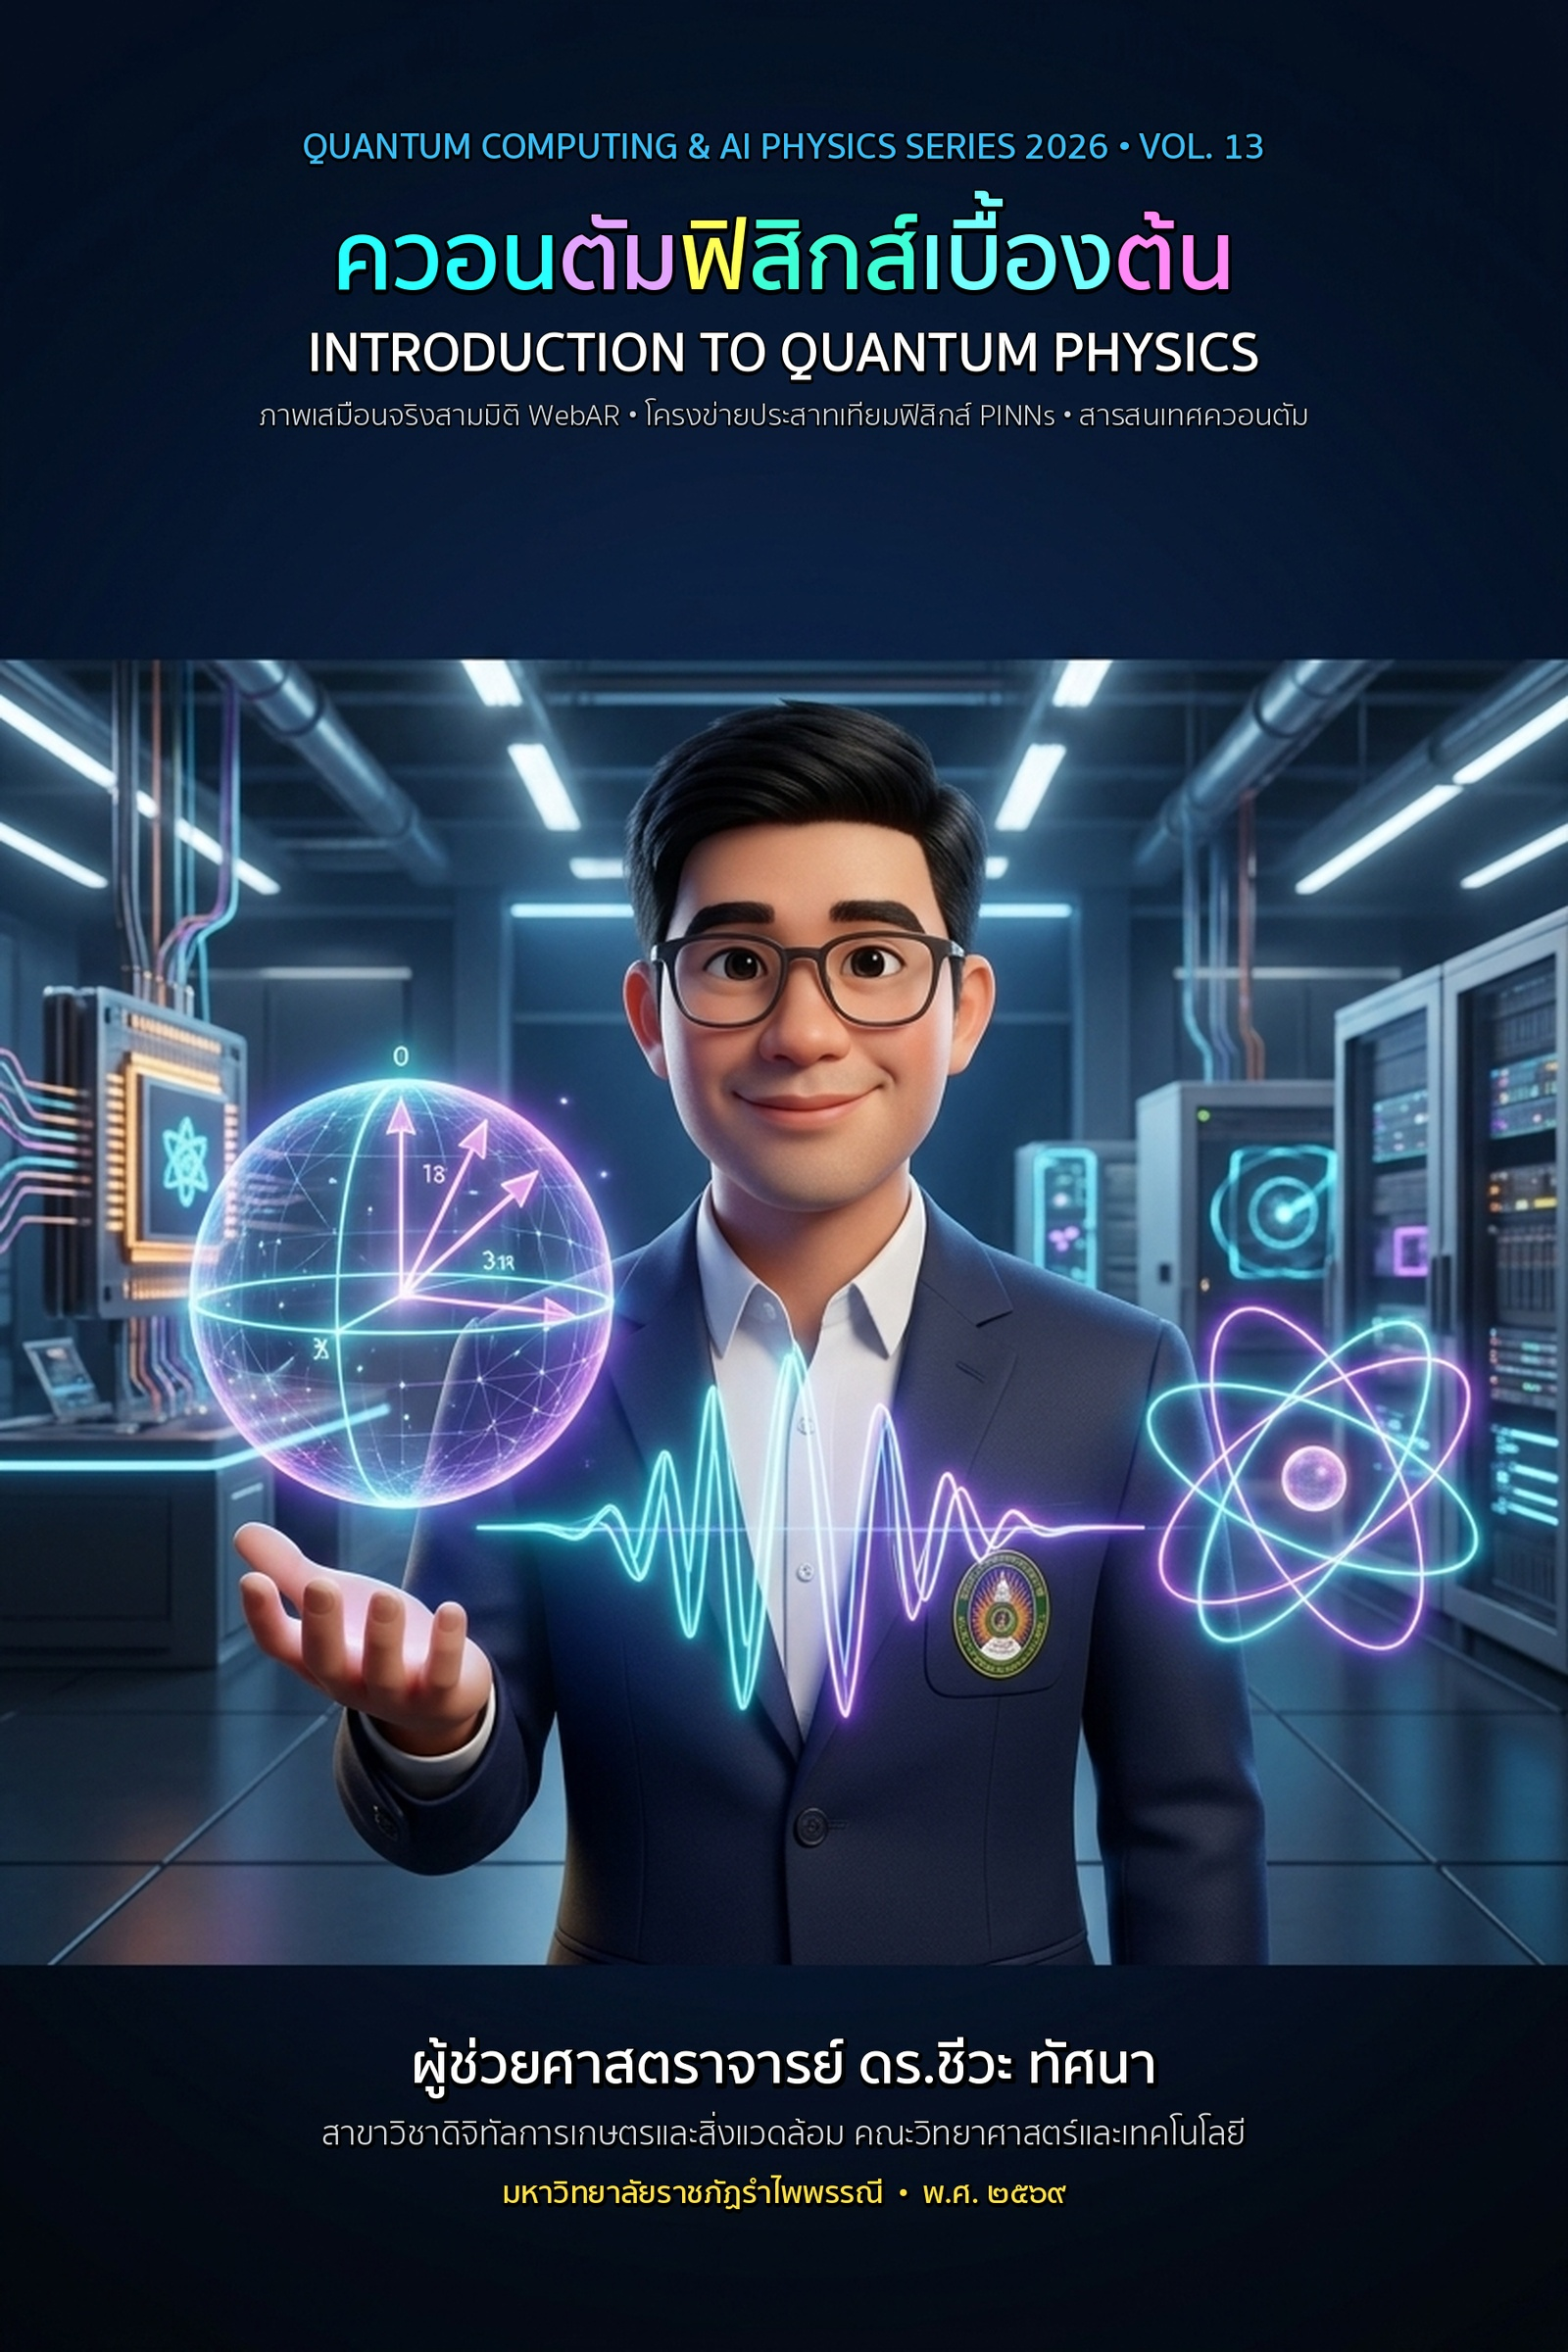
\includegraphics[width=\paperwidth,height=\paperheight]{figures/cover_art_typography.jpg}
    };
\end{tikzpicture}
\clearpage
\restoregeometry
\end{titlepage}

\begin{titlepage}
    \centering
    \vspace*{1.2cm}
    
    {\Huge\bfseries\color{darkNavy} ควอนตัมฟิสิกส์เบื้องต้น \par}
    \vspace{0.4cm}
    {\LARGE\bfseries\color{cyberBlue} การประยุกต์ภาพเสมือนจริงสามมิติและโครงข่ายประสาทเทียมตามหลักฟิสิกส์ \par}
    \vspace{0.35cm}
    {\large\bfseries\color{neonPurple} (Introduction to Quantum Physics: AR/XR Immersive Frameworks and Physics-Informed Neural Networks) \par}
    
    \vspace{1.2cm}
    {\color{quantumGold}\rule{0.85\textwidth}{2pt}}
    \vspace{1.2cm}
    
    {\Large\textbf{ผู้ช่วยศาสตราจารย์ ดร.ชีวะ ทัศนา}\par}
    \vspace{0.35cm}
    {\large วท.บ. (ฟิสิกส์ คอมพิวเตอร์และอิเล็กทรอนิกส์)\par}
    \vspace{0.15cm}
    {\large วท.ม. (ฟิสิกส์ประยุกต์)\par}
    \vspace{0.15cm}
    {\large ปร.ด. (ฟิสิกส์ประยุกต์)\par}
    
    \vfill
    
    {\large สาขาวิชาดิจิทัลการเกษตรและสิ่งแวดล้อม คณะวิทยาศาสตร์และเทคโนโลยี\par}
    \vspace{0.2cm}
    {\large มหาวิทยาลัยราชภัฏรำไพพรรณี\par}
    \vspace{0.2cm}
    {\large จังหวัดจันทบุรี\par}
    \vspace{0.6cm}
    {\large พ.ศ. 2569\par}
\end{titlepage}

\chapter*{คำนำ}
\addcontentsline{toc}{chapter}{คำนำ}

ตำรา \textbf{“ควอนตัมฟิสิกส์เบื้องต้น: การประยุกต์ภาพเสมือนจริงสามมิติและโครงข่ายประสาทเทียมตามหลักฟิสิกส์”} เล่มนี้ เรียบเรียงขึ้นเพื่อใช้ประกอบการเรียนการสอนรายวิชาฟิสิกส์ควอนตัมเบื้องต้น สำหรับนักศึกษาระดับปริญญาตรี คณะวิทยาศาสตร์และเทคโนโลยี มหาวิทยาลัยราชภัฏรำไพพรรณี ตลอดจนสถาบันอุดมศึกษาที่มีการจัดการเรียนการสอนด้านฟิสิกส์ ฟิสิกส์ประยุกต์ วิศวกรรมศาสตร์ และวิทยาการคอมพิวเตอร์

การก้าวเข้าสู่ยุคเทคโนโลยีควอนตัมรุ่นที่สอง (Quantum 2.0) ได้เปลี่ยนกระบวนทัศน์จากการศึกษาพฤติกรรมควอนตัมแบบสังเกตเฉย (Passive Observation) สู่การควบคุมและจัดการสถานะควอนตัมเชิงรุก (Active Manipulation) เช่น ระบบคิวบิต ความพัวพันเชิงควอนตัม และคอมพิวเตอร์ควอนตัม ผู้เขียนจึงได้ปรับปรุงและพัฒนาเนื้อหาในตำราเล่มนี้ให้มีความทันสมัย ครอบคลุมทั้งรากฐานทางทฤษฎีกลศาสตร์คลื่นดั้งเดิม (สมการชเรอดิงเงอร์ บ่อศักย์ ฮาร์มอนิกออสซิลเลเตอร์ อะตอมไฮโดรเจน) และสารสนเทศควอนตัมร่วมสมัย

จุดเด่นสำคัญของตำราเล่มนี้คือการบูรณาการนวัตกรรมการเรียนรู้เชิงรุก (Active Learning) 3 มิติ ได้แก่
\begin{enumerate}
    \item \textbf{ระบบภาพเสมือนจริงสามมิติและการติดตามภาพ (Augmented Reality \& Image Tracking):} ภาพประกอบในหนังสือได้รับการออกแบบให้เป็นเป้าหมายติดตามภาพ (Image Target) นักศึกษาสามารถส่องกล้องสมาร์ทโฟนเข้าหาภาพประกอบเพื่อเรนเดอร์โมเดล 3 มิติเชิงปฏิสัมพันธ์และแอนิเมชันคลื่นลอยตัวเหนือหน้าหนังสือได้ทันทีโดยไม่ต้องติดตั้งแอปพลิเคชัน
    \item \textbf{รหัสตอบสนองเร็วเพื่อเปิดห้องปฏิบัติการเสมือน (Vector QR Code Virtual Labs):} เชื่อมโยงสู่ WebXR 3D Simulator พร้อมระบบตรวจจับมือเปล่า (MediaPipe Hands) ช่วยให้ผู้เรียนสามารถทดลองปรับแต่งตัวแปรทางฟิสิกส์ด้วยมือเปล่าแบบไร้สัมผัส
    \item \textbf{การประมวลผลด้วยปัญญาประดิษฐ์เชิงลึกและภาษา Python (PINNs \& Qiskit):} นำเสนอการประยุกต์โครงข่ายประสาทเทียมตามหลักฟิสิกส์ (Physics-Informed Neural Networks) ในการหาผลเฉลยของสมการชเรอดิงเงอร์ และการจำลองวงจรควอนตัมด้วย Qiskit
\end{enumerate}

ผู้เขียนหวังเป็นอย่างยิ่งว่า ตำราเล่มนี้จะมีส่วนช่วยเปิดมิติใหม่ในการศึกษากลศาสตร์ควอนตัม ทำให้แนวคิดที่เป็นนามธรรมสูงกลายเป็นสิ่งที่จับต้องได้ สร้างแรงบันดาลใจ และเตรียมนักศึกษาให้มีความพร้อมต่อการขับเคลื่อนวิทยาศาสตร์และเทคโนโลยีขั้นสูงของประเทศต่อไป

\vspace{1.5cm}
\begin{flushright}
    ผู้ช่วยศาสตราจารย์ ดร.ชีวะ ทัศนา\\
    สาขาวิชาดิจิทัลการเกษตรและสิ่งแวดล้อม\\
    คณะวิทยาศาสตร์และเทคโนโลยี มหาวิทยาลัยราชภัฏรำไพพรรณี
\end{flushright}

% ==========================================================
% แผนบริหารการสอนรายวิชาควอนตัมฟิสิกส์เบื้องต้น (Course Syllabus)
% ตามกรอบมาตรฐานผลลัพธ์การเรียนรู้ (OBE) มหาวิทยาลัยราชภัฏรำไพพรรณี
% ==========================================================

\chapter*{แผนบริหารการสอนรายวิชา}
\addcontentsline{toc}{chapter}{แผนบริหารการสอนรายวิชา}

\section*{ข้อมูลทั่วไปของรายวิชา}
\noindent\textbf{รหัสและชื่อรายวิชา} ฟิสิกส์ควอนตัมเบื้องต้น (Introduction to Quantum Physics)\\
\noindent\textbf{จำนวนหน่วยกิต} 3(3-0-6) บรรยาย 3 ชั่วโมง ศึกษาค้นคว้าด้วยตนเอง 6 ชั่วโมงต่อสัปดาห์\\
\noindent\textbf{หลักสูตรและประเภทของรายวิชา} วิทยาศาสตรบัณฑิต หมวดวิชาเฉพาะด้านฟิสิกส์ประยุกต์และดิจิทัลการเกษตร\\
\noindent\textbf{อาจารย์ผู้รับผิดชอบรายวิชาและผู้สอน} ผู้ช่วยศาสตราจารย์ ดร.ชีวะ ทัศนา\\
\noindent\textbf{ภาคการศึกษาและชั้นปีที่เรียน} ภาคการศึกษาที่ 1 ชั้นปีที่ 3

\vspace{10pt}
\section*{คำอธิบายรายวิชา}
การกำเนิดของกลศาสตร์ควอนตัม ปรากฏการณ์การแผ่รังสีของวัตถุดำ โฟโตอิเล็กทริก และการกระเจิงคอมป์ตัน ความเป็นทวิภาพของคลื่นและอนุภาค คลื่นสสารเดอ บรอยล์ กลุ่มคลื่นเกาส์เซียน และหลักความไม่แน่นอนของไฮเซนเบิร์ก ปริภูมิฮิลเบิร์ต สัญกรณ์บรา-เคทของดิแรก ตัวดำเนินการแฮร์มิเชียน สมการชเรอดิงเงอร์ที่ขึ้นและไม่ขึ้นกับเวลา การประยุกต์ในบ่อศักย์ กำแพงศักย์ และปรากฏการณ์ทันเนลลิง ตัวแกว่งกวัดฮาร์มอนิกควอนตัมและพีชคณิตตัวดำเนินการบันได อะตอมไฮโดรเจนในระบบพิกัดทรงกลม โมเมนตัมเชิงมุม สปินของอิเล็กตรอนและเมทริกซ์เพาลี ทฤษฎีบทการรบกวน สถิติควอนตัม สารสนเทศควอนตัม คิวบิต ทรงกลมบล็อค เกตควอนตัม ความพัวพันเชิงควอนตัม โพรโทคอลการส่งผ่านสถานะควอนตัมทางไกล อัลกอริทึมควอนตัมเบื้องต้น การจำลองเสมือนจริงสามมิติผ่านเทคโนโลยีภาพเสมือนผสานโลกจริง (AR/XR) และการประยุกต์โครงข่ายประสาทเทียมตามหลักฟิสิกส์ (Physics-Informed Neural Networks) ในการคำนวณเชิงตัวเลข

\vspace{10pt}
\section*{ผลลัพธ์การเรียนรู้ระดับรายวิชา (Course Learning Outcomes: CLOs)}
เมื่อสิ้นสุดการเรียนการสอนรายวิชานี้ นักศึกษาสามารถ
\begin{enumerate}[leftmargin=1.5cm]
    \item \textbf{CLO 1} อธิบายและวิเคราะห์หลักการพื้นฐานทางกลศาสตร์ควอนตัม สัญกรณ์ดิแรก และการแปลงสภาพเชิงเอกภาพได้อย่างถูกต้องตามหลักการทางคณิตศาสตร์และฟิสิกส์
    \item \textbf{CLO 2} แก้สมการชเรอดิงเงอร์สำหรับระบบศักย์หนึ่งมิติ ตัวแกว่งกวัดฮาร์มอนิก และอะตอมไฮโดรเจน พร้อมทั้งตีความฟังก์ชันคลื่นและความน่าจะเป็นได้อย่างถูกต้อง
    \item \textbf{CLO 3} วิเคราะห์และออกแบบวงจรสารสนเทศควอนตัม ระบบคิวบิตบนทรงกลมบล็อค สถานะพัวพันเบลล์ และโพรโทคอลโทรเลขควอนตัมทางไกลได้อย่างเป็นระบบ
    \item \textbf{CLO 4} พัฒนาโปรแกรมภาษา Python ประยุกต์ใช้ Qiskit, QuTiP และโครงข่ายประสาทเทียมตามหลักฟิสิกส์ (PINNs) เพื่อจำลองและหาผลเฉลยของระบบควอนตัมได้อย่างมีประสิทธิภาพ
    \item \textbf{CLO 5} ใช้งานสื่อจำลองเสมือนจริงสามมิติ WebAR ผ่านเทคโนโลยีการติดตามภาพ (Image Tracking) และรหัสตอบสนองเร็ว (QR Code) เพื่อการทดลองเชิงประจักษ์แบบไร้สัมผัส
\end{enumerate}

\newpage
\section*{แผนผังโครงสร้างเนื้อหาและนวัตกรรมการเรียนรู้ประจำบท (Master Syllabus Matrix)}

\begin{table}[H]
\centering
\small
\begin{tabularx}{\textwidth}{c l Y c}
\toprule
\textbf{บทที่} & \textbf{ชื่อบทเรียนภาษาไทย} & \textbf{นวัตกรรมดิจิทัล: AR Target, QR Lab \& Python} & \textbf{CLO} \\
\midrule
1 & สมบัติเชิงอนุภาคของรังสีและโฟตอนิกส์ยุคใหม่ & QR Lab 1: สเปกตรัมวัตถุดำและโฟตอนเดี่ยว\newline Python: Curve Fitting กฎพลังค์เทียบวีน & 1, 4 \\
\addlinespace
2 & ความเป็นทวิภาคคลื่น-อนุภาคและการแทรกสอด & AR Target: ภาพเครื่องมือสลิตคู่อิเล็กตรอน\newline Python: การจำลองการบานออกของ Wave Packet & 1, 4, 5 \\
\addlinespace
3 & สมการชเรอดิงเงอร์และพีชคณิตเชิงเส้นควอนตัม & QR Lab 3: ตัวดำเนินการและการแปลงฐาน Dirac\newline Python: เมทริกซ์แฮร์มิเชียนและค่าไอเกน & 1, 2, 4 \\
\addlinespace
4 & กลศาสตร์คลื่นในบ่อศักย์และปรากฏการณ์ทันเนลลิง & AR Target: ภาพหัวเข็ม STM ระดับอะตอม\newline Python PINNs: แก้บ่อศักย์และจำลองทันเนลลิง & 2, 4, 5 \\
\addlinespace
5 & ตัวแกว่งกวัดฮาร์มอนิกควอนตัมและพีชคณิตตัวดำเนินการ & QR Lab 5: ฟังก์ชัน Wigner และ Coherent State\newline Python QuTiP: ตัวดำเนินการบันได $a, a^\dagger$ & 2, 4 \\
\addlinespace
6 & ระบบอะตอมในสามมิติ โมเมนตัมเชิงมุม และสปิน & AR Target: ภาพออร์บิทัล $3d$ และ $4f$ สามมิติ\newline 3D WebGL: Orbital Viewer หมุนอิสระรอบแกน & 2, 5 \\
\addlinespace
7 & ทฤษฎีการรบกวน สถิติควอนตัม และสสารควอนตัม & QR Lab 7: การแยกของระดับพลังงาน Stark Effect\newline Python: สถิติ Fermi-Dirac และ Bose-Einstein & 2, 4 \\
\addlinespace
8 & สารสนเทศควอนตัม คิวบิต และทรงกลมบล็อค & AR Target: แผนภาพทรงกลมบล็อคสามมิติ\newline Python Qiskit: วงจร 1 คิวบิตและ Statevector & 3, 4, 5 \\
\addlinespace
9 & ความพัวพันเชิงควอนตัมและการสื่อสารควอนตัม & QR Lab 9: การวัดสถานะเบลล์และโทรเลขควอนตัม\newline QR Lab 12: การแจกจ่ายกุญแจรหัสลับควอนตัม QKD\newline Python Qiskit: Teleportation \& QKD BB84 & 3, 4, 5 \\
\addlinespace
10 & อัลกอริทึมควอนตัม คอมพิวติง และพรมแดนประยุกต์ & QR Lab 10: สถาปัตยกรรมชิปควอนตัมและโกรเวอร์\newline QR Lab 11: การแปลงฟูเรียร์ควอนตัม QFT และชอร์\newline Python: Grover Search \& Shor's Factoring & 3, 4, 5 \\
\bottomrule
\end{tabularx}
\caption{โครงสร้างเนื้อหา ผลลัพธ์การเรียนรู้ และนวัตกรรมดิจิทัลประจำบทเรียน}
\end{table}

\vspace{8pt}
\section*{แผนการประเมินผลการเรียนรู้}
การวัดและประเมินผลการเรียนรู้ใช้ระบบการประเมินอิงเกณฑ์ตามมาตรฐานมหาวิทยาลัยราชภัฏรำไพพรรณี แบ่งสัดส่วนคะแนนดังนี้
\begin{enumerate}[leftmargin=1.5cm]
    \item \textbf{การมีส่วนร่วมและการทดลองในชั้นเรียนเสมือนจริง (Interactive Lab Participation)} ร้อยละ 15
    \item \textbf{รายงานปฏิบัติการคอมพิวเตอร์และการเขียนโปรแกรม Python (Computational Lab Reports)} ร้อยละ 20
    \item \textbf{แบบฝึกหัดและการแก้โจทย์ปัญหาเชิงวิเคราะห์แบบ P-S-C-T ประจำบท} ร้อยละ 15
    \item \textbf{การสอบประเมินผลกลางภาคการศึกษา (Midterm Examination)} ร้อยละ 25
    \item \textbf{การสอบประเมินผลปลายภาคการศึกษา (Final Examination)} ร้อยละ 25
\end{enumerate}


% Table of Contents, Figures, Tables
\tableofcontents
\clearpage
\phantomsection
\addcontentsline{toc}{chapter}{\listfigurename}
\listoffigures
\clearpage
\phantomsection
\addcontentsline{toc}{chapter}{\listtablename}
\listoftables

% Mainmatter: 10 Core Chapters
\mainmatter
\chapter{สมบัติเชิงอนุภาคของรังสีและโฟตอนิกส์ยุคใหม่}
\label{chap:particle_properties}
\index{การแผ่รังสีวัตถุดำ (Blackbody Radiation)}
\index{ปรากฏการณ์โฟโตอิเล็กทริก (Photoelectric Effect)}
\index{การกระเจิงคอมป์ตัน (Compton Scattering)}
\index{โฟตอน (Photon)}
\index{โฟตอนิกส์ (Photonics)}
\index{การสร้างคู่ (Pair Production)}
\index{การประลัย (Annihilation)}
\index{เครื่องชั่งคิบเบิล (Kibble Balance)}
\index{ตัวตรวจวัดโฟตอนเดี่ยวตัวนำยิ่งยวด (SNSPD)}

% ==========================================================
% แผนบริหารการสอนประจำบทที่ 1
% ==========================================================
\section*{แผนบริหารการสอนประจำบทที่ 1}
\addcontentsline{toc}{section}{แผนบริหารการสอนประจำบทที่ 1}

\begin{lessonplanbox}
\noindent\textbf{หัวข้อเนื้อหาประจำบท}
\begin{enumerate}
    \item ภูมิหลังทางประวัติศาสตร์และวิกฤตการณ์ฟิสิกส์คลาสสิกช่วงปลายคริสต์ศตวรรษที่ 19
    \item ฟิสิกส์ของการแผ่รังสีวัตถุดำ โหมดคลื่นนิ่งในโพรง และกฎของเรย์ลีห์-จีนส์
    \item การอนุพัทธ์กฎของพลังค์ฉบับสมบูรณ์และสมมติฐานการควอนไตซ์พลังงาน
    \item การพิสูจน์กฎการกระจัดของวีน กฎสเตฟาน-โบลทซ์มัน และอุณหพลศาสตร์ของก๊าซโฟตอน
    \item ปรากฏการณ์โฟโตอิเล็กทริก การทดลองของเลนนาร์ด และสมมติฐานโฟตอนของไอน์สไตน์
    \item ข้อจำกัดของทฤษฎีคลื่นคลาสสิก การทดลองอันแม่นยำของมิลลิแกน และฟังก์ชันงาน
    \item การกระเจิงคอมป์ตัน จลนศาสตร์สัมพัทธภาพฉบับเต็ม และการกระเจิงคอมป์ตันย้อนกลับ
    \item การสร้างคู่อนุภาค-ปฏิอนุภาค เงื่อนไขอนุรักษ์โมเมนตัม โพซิตโรเนียม และการประลัย
    \item พรมแดนงานวิจัยร่วมสมัย ---- เครื่องชั่งคิบเบิล การนิยามระบบหน่วยเอสไอใหม่ ตัวตรวจวัด SNSPD และโซลาร์เซลล์เพอรอฟสไกต์ควอนตัมดอต
    \item ห้องปฏิบัติการเสมือนจริง WebAR การจำลองเชิงตัวเลขด้วย Python และการประยุกต์ P-S-C-T
\end{enumerate}

\noindent\textbf{วัตถุประสงค์เชิงพฤติกรรม}
\begin{enumerate}
    \item อธิบายกลไกการเกิดวิกฤตการณ์อัลตราไวโอเลต และอนุพัทธ์ความหนาแน่นของโหมดคลื่นนิ่งในโพรงสามมิติได้อย่างถูกต้องตามหลักการทางคณิตศาสตร์
    \item อนุพัทธ์กฎของพลังค์ กฎการกระจัดของวีน และกฎสเตฟาน-โบลทซ์มัน จากระเบียบวิธีกลศาสตร์สถิติควอนตัมได้อย่างเป็นระบบ
    \item คำนวณพลังงานจลน์สูงสุด ศักย์หยุดยั้ง และอธิบายการคำนวณความล่าช้าเชิงเวลาในทฤษฎีคลื่นคลาสสิกเทียบกับข้อเท็จจริงเชิงควอนตัมได้อย่างลึกซึ้ง
    \item แก้ปัญหาจลนศาสตร์สัมพัทธภาพของการกระเจิงคอมป์ตันและการสร้างคู่ในระบบ 4-โมเมนตัมได้อย่างแม่นยำ
    \item ประยุกต์ความรู้ฟิสิกส์ควอนตัมเชิงอนุภาคเข้ากับการวิเคราะห์เทคโนโลยีมาตรวิทยาขั้นสูง (เครื่องชั่งคิบเบิล) และเทคโนโลยีโฟตอนิกส์ยุคปัจจุบัน พร้อมพัฒนาโปรแกรมจำลองผลเชิงตัวเลขได้
\end{enumerate}
\end{lessonplanbox}

% ==========================================================
% 1.1 ภูมิหลังทางประวัติศาสตร์และวิกฤตการณ์ฟิสิกส์คลาสสิก
% ==========================================================
\newpage
\section{ภูมิหลังทางประวัติศาสตร์และวิกฤตการณ์ฟิสิกส์คลาสสิก}
\index{วิกฤตการณ์อัลตราไวโอเลต (Ultraviolet Catastrophe)}
\index{เมฆหมอกสองก้อนของเคลวิน (Kelvin's Two Clouds)}

ในช่วงปลายคริสต์ศตวรรษที่ 19 ประชาคมนักฟิสิกส์มีความเชื่อมั่นเป็นอย่างยิ่งว่า โครงสร้างพื้นฐานของฟิสิกส์มีความสมบูรณ์และครอบคลุมปรากฏการณ์ธรรมชาติทั้งหมดแล้ว โดยมีเสาหลักสามประการที่ค้ำจุนจักรวาลเชิงทฤษฎี ได้แก่

\begin{enumerate}
    \item \textbf{กลศาสตร์นิวโตเนียน (Newtonian Mechanics)} ---- ที่พัฒนาต่อยอดโดยลากรองจ์ (Lagrange) และแฮมิลตัน (Hamilton) ซึ่งสามารถทำนายการเคลื่อนที่ของอนุภาคและวัตถุท้องฟ้าได้อย่างแม่นยำยิ่ง
    \item \textbf{ทฤษฎีแม่เหล็กไฟฟ้าของแมกซ์เวลล์ (Maxwell's Electrodynamics)} ---- ซึ่งรวมปรากฏการณ์ทางไฟฟ้า แม่เหล็ก และทัศนศาสตร์ เข้าด้วยกันผ่านสมการคลื่นแม่เหล็กไฟฟ้า
    \item \textbf{อุณหพลศาสตร์และกลศาสตร์สถิติ (Thermodynamics and Statistical Mechanics)} ---- นำโดยคาร์โนต์ (Carnot) เคลาซิอุส (Clausius) เคลวิน (Kelvin) และโบลทซ์มัน (Boltzmann) ที่อธิบายพฤติกรรมของสสารในระดับมหภาคผ่านการเคลื่อนที่เชิงสถิติของโมเลกุล
\end{enumerate}

ในคริสต์ศักราช 1900 ลอร์ดเคลวิน (Lord Kelvin หรือ William Thomson, 1824--1907) ได้กล่าวปาฐกถาอันมีชื่อเสียงต่อหน้าราชสมาคมแห่งเกรตบริเตน (Royal Institution of Great Britain) ความว่า บิวตี้และความชัดเจนของทฤษฎีพลศาสตร์ที่อธิบายความร้อนและแสงสว่างกำลังถูกบดบังด้วย \textbf{เมฆหมอกสองก้อน (Two Clouds on the Horizon of Physics)} ก้อนแรกคือ ผลการทดลองของไมเคิลสัน-มอร์ลีย์ (Michelson-Morley Experiment) ที่ตรวจไม่พบการเคลื่อนที่สัมพัทธ์ของอีเทอร์ ซึ่งนำไปสู่ทฤษฎีสัมพัทธภาพพิเศษของไอน์สไตน์ในเวลาต่อมา และก้อนที่สองคือ ความล้มเหลวของทฤษฎีบทการแบ่งเท่าพลังงาน (Equipartition Theorem) ในการอธิบายการแผ่รังสีความร้อนของวัตถุดำและความจุความร้อนจำเพาะของก๊าซและของแข็งที่อุณหภูมิต่ำ

วิกฤตการณ์ของฟิสิกส์คลาสสิกไม่ได้เกิดขึ้นจากความบกพร่องทางคณิตศาสตร์ หากแต่เกิดจากข้อจำกัดพื้นฐานของกระบวนทัศน์ดั้งเดิมที่สันนิษฐานว่า \textbf{พลังงานและการถ่ายโอนพลังงานในธรรมชาติมีลักษณะต่อเนื่อง (Continuous)} ความขัดแย้งที่ไม่อาจประนีประนอมได้นี้ ได้นำไปสู่การก่อกำเนิดของกลศาสตร์ควอนตัม โดยเริ่มต้นจากการไขปริศนาการแผ่รังสีของวัตถุดำ

% ==========================================================
% 1.2 การแผ่รังสีวัตถุดำและกฎของเรย์ลีห์-จีนส์
% ==========================================================
\section{การแผ่รังสีวัตถุดำและกฎของเรย์ลีห์-จีนส์}
\index{วัตถุดำ (Blackbody)}
\index{กฎของเรย์ลีห์-จีนส์ (Rayleigh-Jeans Law)}
\index{ความหนาแน่นของโหมด (Density of States)}

\subsection{ธรรมชาติของวัตถุดำและแบบจำลองโพรงรังสี}

วัตถุทุกชนิดที่มีอุณหภูมิสูงกว่าศูนย์สัมบูรณ์ ($T > 0~\text{K}$) จะแผ่คลื่นแม่เหล็กไฟฟ้าออกมาอย่างต่อเนื่อง เนื่องจากการสั่นไหวทางความร้อนของอนุภาคที่มีประจุไฟฟ้าภายในเนื้อสสาร \textbf{วัตถุดำอุดมคติ (Ideal Blackbody)} นิยามโดย กุสทัฟ เคียร์ชฮอฟฟ์ (Gustav Kirchhoff, 1824--1887) ในคริสต์ศักราช 1859 ว่าเป็นวัตถุที่ดูดกลืนรังสีแม่เหล็กไฟฟ้าทุกความถี่ที่ตกกระทบได้อย่างสมบูรณ์ โดยไม่มีการสะท้อนหรือทะลุผ่าน ($\alpha(\nu) = 1$ ทุกความถี่)

จากกฎการแผ่รังสีของเคียร์ชฮอฟฟ์ (Kirchhoff's Law of Thermal Radiation) อัตราส่วนระหว่างสภาพเปล่งรังสี ($e(\nu, T)$) ต่อสภาพดูดกลืนรังสี ($\alpha(\nu, T)$) ของวัตถุใด ๆ ที่อยู่ในสมดุลความร้อนจะมีค่าเท่ากันเสมอ และมีค่าเท่ากับสภาพเปล่งรังสีของวัตถุดำ ($e_b(\nu, T)$) ซึ่งขึ้นกับความถี่และอุณหภูมิเท่านั้น โดยไม่ขึ้นกับรูปร่าง ขนาด หรือชนิดของวัสดุ

\begin{equation}
\frac{e(\nu, T)}{\alpha(\nu, T)} = e_b(\nu, T)
\label{eq:kirchhoff_law}
\end{equation}

ในทางปฏิบัติ แบบจำลองที่ดีที่สุดของวัตถุดำคือ \textbf{โพรงกลวงที่มีรูเปิดขนาดเล็กมาก (Cavity Radiator)} ดังแสดงในภาพที่~\ref{fig:blackbody_cavity} เมื่อรังสีแม่เหล็กไฟฟ้าภายนอกลอดผ่านรูเปิดขนาดเล็กเข้าไปในโพรง รังสีจะสะท้อนไปมาระหว่างผนังภายในหลายครั้ง ในการสะท้อนแต่ละครั้ง ผนังจะดูดกลืนพลังงานรังสีไปบางส่วน เมื่อสะท้อนซ้ำไปซ้ำมา รังสีจะถูกดูดกลืนจนหมดเกลี้ยง โอกาสที่รังสีจะสะท้อนลอดกลับออกมาทางรูเปิดมีค่าน้อยมากจนเข้าใกล้ศูนย์ ดังนั้น รูเปิดของโพรงจึงทำหน้าที่เป็นพื้นผิวของวัตถุดำอุดมคติที่ดูดกลืนรังสีได้อย่างสมบูรณ์ และรังสีที่แผ่ออกมาจากรูเปิดเมื่อผนังโพรงได้รับความร้อนจนเข้าสู่สมดุลความร้อน ก็คือ \textbf{การแผ่รังสีของวัตถุดำ (Blackbody Radiation)}

\begin{figure}[H]
\centering
\begin{tikzpicture}[scale=1.1]
    % Outer cavity shell
    \draw[line width=3pt, darkNavy, fill=slateGrey!20] (0, 0) circle (2.8cm);
    \fill[white] (-2.8, -0.4) rectangle (-2.7, 0.4); % Entrance aperture
    
    % Cavity interior
    \fill[black!90] (0, 0) circle (2.5cm);
    \draw[line width=1.5pt, cyberBlue] (0,0) circle (2.5cm);

    % Multiple reflection path
    \draw[-{Stealth}, line width=1.4pt, quantumGold] (-4.0, 0.2) -- (-2.7, 0.2);
    \draw[-{Stealth}, line width=1.2pt, quantumGold] (-2.7, 0.2) -- (1.5, 1.8);
    \draw[-{Stealth}, line width=1.2pt, quantumGold] (1.5, 1.8) -- (2.2, -0.8);
    \draw[-{Stealth}, line width=1.1pt, quantumGold] (2.2, -0.8) -- (-0.8, -2.2);
    \draw[-{Stealth}, line width=1.0pt, quantumGold] (-0.8, -2.2) -- (-1.8, -1.2);
    \draw[-{Stealth}, line width=0.8pt, quantumGold] (-1.8, -1.2) -- (0.5, -0.5);

    % Aperture label
    \draw[-{Stealth}, neonPurple, line width=1.2pt] (-3.8, 1.5) -- (-2.8, 0.3);
    \node at (-4.2, 1.8) [font=\small\bfseries\color{neonPurple}] {รูเปิดขนาดเล็ก (Aperture)};

    % Cavity label
    \node at (0, 0.8) [font=\bfseries\color{white}] {สนามรังสีในสมดุลความร้อน};
    \node at (0, 0.2) [font=\small\color{cyan}] {$T = \text{const}$};
    \node at (0, -0.5) [font=\footnotesize\color{slateGrey!50}] {ผนังดูดกลืนและเปล่งรังสี};
\end{tikzpicture}
\caption{แบบจำลองโพรงรังสีวัตถุดำ แสดงการสะท้อนภายในหลายครั้งจนรังสีถูกดูดกลืนอย่างสมบูรณ์ และรังสีที่เปล่งออกจากรูเปิดคือรังสีวัตถุดำ}
\label{fig:blackbody_cavity}
\end{figure}

\subsection{การอนุพัทธ์ความหนาแน่นของโหมดคลื่นนิ่งในโพรงสามมิติ}

พิจารณาโพรงสุญญากาศรูปลูกบาศก์ที่มีความยาวด้านละ $L$ มีปริมาตร $V = L^3$ ผนังทุกด้านเป็นตัวนำไฟฟ้าสมบูรณ์ สนามแม่เหล็กไฟฟ้าภายในโพรงจะสะท้อนกลับไปมาระหว่างผนังและเกิดการแทรกสอดจนกลายเป็น \textbf{คลื่นนิ่งแม่เหล็กไฟฟ้า (Electromagnetic Standing Waves)} 

เงื่อนไขขอบเขตสำหรับสนามไฟฟ้าสัมผัสกับผนังตัวนำสมบูรณ์คือ $E_{\parallel} = 0$ ที่ผนัง $x = 0, L$ และ $y = 0, L$ และ $z = 0, L$ ส่งผลให้เวกเตอร์คลื่น $\vec{k} = (k_x, k_y, k_z)$ ถูกจำกัดค่าตามเงื่อนไข

\begin{equation}
k_x = \frac{n_x \pi}{L}, \quad k_y = \frac{n_y \pi}{L}, \quad k_z = \frac{n_z \pi}{L}
\label{eq:wavevector_components}
\end{equation}

โดยที่ $n_x, n_y, n_z$ เป็นจำนวนเต็มบวก ($1, 2, 3, \dots$) ความถี่ของการแกว่งกวัดสัมพันธ์กับขนาดของเวกเตอร์คลื่นตามสมการการกระจายตัวของคลื่นแม่เหล็กไฟฟ้าในสุญญากาศ

\begin{equation}
\nu = \frac{c k}{2\pi} = \frac{c}{2\pi}\sqrt{k_x^2 + k_y^2 + k_z^2} = \frac{c}{2L}\sqrt{n_x^2 + n_y^2 + n_z^2}
\label{eq:frequency_modes}
\end{equation}

นิยามรัศมีในปริภูมิจำนวนเต็ม $n = \sqrt{n_x^2 + n_y^2 + n_z^2} = \frac{2L\nu}{c}$ จำนวนโหมดทั้งหมดที่มีความถี่น้อยกว่าหรือเท่ากับ $\nu$ สอดคล้องกับปริมาตรของทรงกลมหนึ่งในแปด (Octant) ในปริภูมิ $n$-space (เนื่องจาก $n_x, n_y, n_z > 0$) คูณด้วย 2 เพื่อคิดรวมสถานะโพลาไรเซชันอิสระสองสถานะของคลื่นแม่เหล็กไฟฟ้าตามขวาง

\begin{equation}
N(\nu) = 2 \times \frac{1}{8} \times \left( \frac{4}{3}\pi n^3 \right) = \frac{\pi}{3} n^3 = \frac{\pi}{3} \left( \frac{2L\nu}{c} \right)^3 = \frac{8\pi L^3}{3 c^3} \nu^3 = \frac{8\pi V}{3 c^3} \nu^3
\label{eq:total_modes}
\end{equation}

จำนวนโหมดคลื่นนิ่งต่อหน่วยปริมาตรในช่วงความถี่ระหว่าง $\nu$ ถึง $\nu + d\nu$ คือ \textbf{ความหนาแน่นของโหมด (Density of States, $g(\nu)$)} หาได้จากการหาอนุพันธ์ของ $N(\nu)/V$ เทียบกับ $\nu$

\begin{equation}
g(\nu) d\nu = \frac{1}{V}\frac{dN}{d\nu} d\nu = \frac{8\pi\nu^2}{c^3} d\nu
\label{eq:density_of_states}
\end{equation}

หากพิจารณาในเทอมของความยาวคลื่น $\lambda$ โดยใช้ความสัมพันธ์ $\nu = c/\lambda$ และ $|d\nu| = (c/\lambda^2)d\lambda$ จะได้ความหนาแน่นของโหมดต่อหน่วยความยาวคลื่น

\begin{equation}
g(\lambda) d\lambda = \frac{8\pi}{\lambda^4} d\lambda
\label{eq:density_of_states_lambda}
\end{equation}

สมการ~\eqref{eq:density_of_states} และ~\eqref{eq:density_of_states_lambda} เป็นผลลัพธ์เชิงเรขาคณิตและทฤษฎีคลื่นคลาสสิกที่ถูกต้องสมบูรณ์ และไม่มีข้อโต้แย้งใด ๆ ในทางฟิสิกส์

\subsection{ทฤษฎีบทการแบ่งเท่าพลังงานและความล้มเหลวของกฎเรย์ลีห์-จีนส์}

ในการหาความหนาแน่นพลังงานเชิงสเปกตรัม $u(\nu, T)$ ฟิสิกส์คลาสสิกอาศัย \textbf{ทฤษฎีบทการแบ่งเท่าพลังงาน (Equipartition Theorem)} ของวิลเลียม ทอมสัน และเจมส์ เคลิร์ก แมกซ์เวลล์ ซึ่งระบุว่า สำหรับระบบที่อยู่ในสมดุลความร้อนที่อุณหภูมิสัมบูรณ์ $T$ ระดับขั้นความเสรีเชิงกำลังสอง (Quadratic Degree of Freedom) แต่ละระดับจะมีพลังงานเฉลี่ยเท่ากับ $\frac{1}{2}k_B T$

เนื่องจากคลื่นนิ่งแม่เหล็กไฟฟ้าแต่ละโหมดเทียบเท่ากับตัวแกว่งกวัดฮาร์มอนิกอย่างง่าย (Simple Harmonic Oscillator) ที่มีทั้งพลังงานจลน์ (สนามแม่เหล็ก) และพลังงานศักย์ (สนามไฟฟ้า) จึงมีระดับขั้นความเสรีสองระดับ พลังงานเฉลี่ยของแต่ละโหมดในทางคลาสสิกจึงมีค่าเท่ากับ

\begin{equation}
\langle \varepsilon \rangle_{\text{classical}} = \frac{1}{2}k_B T + \frac{1}{2}k_B T = k_B T
\label{eq:classical_mean_energy}
\end{equation}

เมื่อนำพลังงานเฉลี่ยไปคูณกับความหนาแน่นของโหมด จะได้ \textbf{กฎการแผ่รังสีของเรย์ลีห์-จีนส์ (Rayleigh-Jeans Law)} ที่เสนอในคริสต์ศักราช 1900 และปรับปรุงในคริสต์ศักราช 1905

\begin{equation}
u(\nu, T) d\nu = g(\nu) \langle \varepsilon \rangle_{\text{classical}} d\nu = \frac{8\pi\nu^2}{c^3} k_B T d\nu
\label{eq:rayleigh_jeans_full}
\end{equation}

หรือในรูปของความยาวคลื่น

\begin{equation}
u(\lambda, T) d\lambda = \frac{8\pi k_B T}{\lambda^4} d\lambda
\label{eq:rayleigh_jeans_lambda_full}
\end{equation}

พิจารณาผลลัพธ์ของสมการ~\eqref{eq:rayleigh_jeans_full} เมื่อคำนวณพลังงานรวมทั้งหมดต่อหน่วยปริมาตรของรังสีในโพรง โดยการอินทิเกรตตลอดทุกช่วงความถี่ตั้งแต่ศูนย์ถึงอนันต์

\begin{equation}
u_{\text{total}} = \int_0^\infty u(\nu, T) d\nu = \frac{8\pi k_B T}{c^3} \int_0^\infty \nu^2 d\nu = \infty
\label{eq:uv_catastrophe_integral}
\end{equation}

ผลลัพธ์ที่เป็นอนันต์นี้ ชี้ว่าวัตถุที่อุณหภูมิใด ๆ เหนือศูนย์สัมบูรณ์จะแผ่รังสีพลังงานสูง (ย่านอัลตราไวโอเลต รังสีเอกซ์ และรังสีแกมมา) ออกมาอย่างมหาศาลไม่สิ้นสุด ซึ่งขัดแย้งกับการทดลองและการดำรงอยู่ของสสารในเอกภพอย่างสิ้นเชิง ความล้มเหลวเชิงทฤษฎีนี้ถูกขนานนามโดย พอล เอห์เรนเฟสต์ (Paul Ehrenfest, 1880--1933) ว่า \textbf{วิกฤตการณ์อัลตราไวโอเลต (Ultraviolet Catastrophe)}

% ==========================================================
% 1.3 การอนุพัทธ์กฎของพลังค์ฉบับสมบูรณ์
% ==========================================================
\section{การอนุพัทธ์กฎของพลังค์ฉบับสมบูรณ์และสมมติฐานควอนตัม}
\index{กฎของพลังค์ (Planck's Law)}
\index{การควอนไตซ์พลังงาน (Energy Quantization)}
\index{ค่าคงตัวพลังค์ (Planck's Constant)}

\subsection{สมมติฐานการควอนไตซ์พลังงานของพลังค์}

มัคซ์ พลังค์ (Max Planck) ตระหนักว่าปัญหาไม่ได้อยู่ที่การนับจำนวนโหมด $g(\nu)$ แต่อยู่ที่การคำนวณพลังงานเฉลี่ย $\langle \varepsilon \rangle$ ของตัวแกว่งกวัด พลังค์จึงได้ตั้งสมมติฐานอันกล้าหาญเมื่อวันที่ 14 ธันวาคม คริสต์ศักราช 1900 ซึ่งถือเป็นวันกำเนิดของฟิสิกส์ควอนตัม โดยระบุว่า

\begin{quote}
\textit{ตัวแกว่งกวัดของอะตอมในผนังโพรง ไม่สามารถดูดกลืนหรือปลดปล่อยพลังงานได้อย่างต่อเนื่องตามใจชอบ หากแต่พลังงานของตัวแกว่งกวัดจะต้องถูกจำกัดให้อยู่ในรูปของกลุ่มก้อนพลังงานย่อยที่เรียกว่า ควอนตัม (Quantum) โดยเป็นจำนวนเต็มเท่าของปริมาณพลังงานมูลฐาน $h\nu$}
\end{quote}

\begin{equation}
\varepsilon_n = n h\nu = n \hbar \omega, \quad n = 0, 1, 2, 3, \dots
\label{eq:planck_energy_levels}
\end{equation}

โดยที่ $h = 6.62607015 \times 10^{-34}~\text{J}\cdot\text{s}$ คือ \textbf{ค่าคงตัวพลังค์ (Planck's Constant)} ซึ่งเป็นค่าคงตัวมูลฐานของเอกภพ และ $\hbar = h/(2\pi) = 1.054571817 \times 10^{-34}~\text{J}\cdot\text{s}$ คือค่าคงตัวพลังค์ลด (Reduced Planck Constant หรือ Dirac Constant)

\subsection{การคำนวณพลังงานเฉลี่ยตามสถิติของโบลทซ์มัน}

ในสถิติแบบดั้งเดิมของแมกซ์เวลล์-โบลทซ์มัน โอกาสที่ตัวแกว่งกวัดจะมีพลังงาน $\varepsilon_n$ แปรผันตามตัวคูณโบลทซ์มัน $e^{-\varepsilon_n / (k_B T)} = e^{-n h\nu / (k_B T)}$ นิยามตัวแปรเสริม $\beta = \frac{1}{k_B T}$ และกำหนดให้ $x = \beta h\nu = \frac{h\nu}{k_B T}$

ฟังก์ชันแบ่งส่วน (Partition Function, $Z$) ของตัวแกว่งกวัดหนึ่งตัวคำนวณได้จากการบวกผลรวมอนันต์ของอนุกรมเรขาคณิต

\begin{equation}
Z = \sum_{n=0}^\infty e^{-n \beta h\nu} = \sum_{n=0}^\infty \left( e^{-\beta h\nu} \right)^n = \frac{1}{1 - e^{-\beta h\nu}}
\label{eq:partition_function}
\end{equation}

พลังงานเฉลี่ย $\langle \varepsilon \rangle$ คำนวณได้จากนิยามค่าคาดหมายทางสถิติ

\begin{equation}
\langle \varepsilon \rangle = \frac{\sum_{n=0}^\infty \varepsilon_n e^{-\beta \varepsilon_n}}{\sum_{n=0}^\infty e^{-\beta \varepsilon_n}} = -\frac{1}{Z}\frac{\partial Z}{\partial \beta} = -\frac{\partial}{\partial \beta}\ln Z
\label{eq:mean_energy_derivation_1}
\end{equation}

แทนค่า $Z$ จากสมการ~\eqref{eq:partition_function} ลงในสมการ~\eqref{eq:mean_energy_derivation_1}

\begin{align}
\langle \varepsilon \rangle &= -\frac{\partial}{\partial \beta} \ln \left( \frac{1}{1 - e^{-\beta h\nu}} \right) = \frac{\partial}{\partial \beta} \ln \left( 1 - e^{-\beta h\nu} \right) \nonumber \\
&= \frac{1}{1 - e^{-\beta h\nu}} \cdot \left( -e^{-\beta h\nu} \right) \cdot (-h\nu) \nonumber \\
&= \frac{h\nu e^{-\beta h\nu}}{1 - e^{-\beta h\nu}} = \frac{h\nu}{e^{\beta h\nu} - 1}
\label{eq:mean_energy_derivation_2}
\end{align}

ดังนั้น พลังงานเฉลี่ยของตัวแกว่งกวัดควอนตัมที่มีความถี่ $\nu$ ณ อุณหภูมิ $T$ คือ

\begin{equation}
\langle \varepsilon \rangle_{\text{Planck}} = \frac{h\nu}{e^{h\nu / (k_B T)} - 1}
\label{eq:planck_mean_energy}
\end{equation}

\subsection{การวิเคราะห์พฤติกรรมของพลังงานเฉลี่ยในสองขีดจำกัด}

เมื่อพิจารณาสมการ~\eqref{eq:planck_mean_energy} ในช่วงขีดจำกัดทางกายภาพที่แตกต่างกัน

\begin{enumerate}
    \item \textbf{ขีดจำกัดความถี่ต่ำ หรือ อุณหภูมิสูง ($h\nu \ll k_B T$ หรือ $x \ll 1$)} \\
    กระจายฟังก์ชันเลขชี้กำลังด้วยอนุกรมเทย์เลอร์ $e^x = 1 + x + \frac{x^2}{2!} + \dots \approx 1 + x$
    \begin{equation}
    \langle \varepsilon \rangle \approx \frac{h\nu}{(1 + \frac{h\nu}{k_B T}) - 1} = \frac{h\nu}{\frac{h\nu}{k_B T}} = k_B T
    \end{equation}
    พลังงานเฉลี่ยลดรูปกลับไปเป็นผลลัพธ์ของฟิสิกส์คลาสสิกตามทฤษฎีบทการแบ่งเท่าพลังงาน ซึ่งอธิบายว่าเหตุใดกฎของเรย์ลีห์-จีนส์จึงใช้ได้ดีเฉพาะในย่านความถี่ต่ำ (คลื่นวิทยุและอินฟราเรดไกล)
    
    \item \textbf{ขีดจำกัดความถี่สูง หรือ อุณหภูมิต่ำ ($h\nu \gg k_B T$ หรือ $x \gg 1$)} \\
    ในกรณีนี้ $e^{h\nu/(k_B T)} \gg 1$ ทำให้ตัดเลข 1 ในตัวส่วนทิ้งได้
    \begin{equation}
    \langle \varepsilon \rangle \approx h\nu e^{-h\nu / (k_B T)} \xrightarrow{\nu \to \infty} 0
    \end{equation}
    พลังงานเฉลี่ยจะลดลงอย่างรวดเร็วในลักษณะเอ็กซ์โพเนนเชียลเข้าสู่ศูนย์เมื่อความถี่สูงขึ้น เนื่องจากขนาดของควอนตัมพลังงาน $h\nu$ มีค่าใหญ่โตมหาศาลเกินกว่าที่พลังงานความร้อนเฉลี่ย $k_B T$ จะสามารถกระตุ้นให้ตัวแกว่งกวัดเปลี่ยนสถานะขึ้นไปครอบครองระดับพลังงานนั้นได้ ปรากฏการณ์นี้เรียกว่า \textbf{การแช่แข็งของระดับขั้นความเสรี (Freezing out of degrees of freedom)} ซึ่งช่วยกำจัดวิกฤตการณ์อัลตราไวโอเลตได้อย่างหมดจด
\end{enumerate}

\subsection{สมการการกระจายพลังงานของพลังค์}

เมื่อนำความหนาแน่นของโหมด $g(\nu)$ จากสมการ~\eqref{eq:density_of_states} มาคูณกับพลังงานเฉลี่ยตามควอนตัม $\langle \varepsilon \rangle_{\text{Planck}}$ จากสมการ~\eqref{eq:planck_mean_energy} จะได้ \textbf{กฎการแผ่รังสีของพลังค์ (Planck's Radiation Law)}

\begin{equation}
u(\nu, T) d\nu = \frac{8\pi h\nu^3}{c^3} \frac{1}{e^{h\nu/(k_B T)} - 1} d\nu
\label{eq:planck_spectrum_nu}
\end{equation}

ในการแปลงเป็นฟังก์ชันของความยาวคลื่น $u(\lambda, T)$ ต้องใช้เงื่อนไขการอนุรักษ์ความหนาแน่นพลังงาน $u(\lambda, T)|d\lambda| = u(\nu, T)|d\nu|$ โดยที่ $\nu = c/\lambda$ และ $d\nu = -\frac{c}{\lambda^2}d\lambda$

\begin{equation}
u(\lambda, T) = u(\nu, T) \left| \frac{d\nu}{d\lambda} \right| = \frac{8\pi h(c/\lambda)^3}{c^3} \frac{1}{e^{hc/(\lambda k_B T)} - 1} \left( \frac{c}{\lambda^2} \right)
\end{equation}

\begin{equation}
u(\lambda, T) d\lambda = \frac{8\pi h c}{\lambda^5} \frac{1}{e^{hc/(\lambda k_B T)} - 1} d\lambda
\label{eq:planck_spectrum_lambda}
\end{equation}

สำหรับสภาพเปล่งรังสีสเปกตรัมต่อหน่วยพื้นที่ผิว $I(\lambda, T)$ (Spectral Radiance) สัมพันธ์กับความหนาแน่นพลังงานในโพรงตามความสัมพันธ์เชิงทัศนศาสตร์ $I(\lambda, T) = \frac{c}{4\pi} u(\lambda, T)$ หรือหากพิจารณากำลังการแผ่รังสีที่เปล่งออกสู่ครึ่งทรงกลมด้านหน้า (Hemispherical Emissive Power) $R(\lambda, T) = \frac{c}{4} u(\lambda, T)$ จะได้

\begin{equation}
R(\lambda, T) = \frac{2\pi h c^2}{\lambda^5} \frac{1}{e^{hc/(\lambda k_B T)} - 1}
\label{eq:planck_radiance_R}
\end{equation}

% ==========================================================
% 1.4 การพิสูจน์กฎการกระจัดของวีนและกฎสเตฟาน-โบลทซ์มัน
% ==========================================================
\section{การพิสูจน์กฎการกระจัดของวีนและกฎสเตฟาน-โบลทซ์มัน}
\index{กฎการกระจัดของวีน (Wien's Displacement Law)}
\index{กฎสเตฟาน-โบลทซ์มัน (Stefan-Boltzmann Law)}
\index{ความดันการแผ่รังสี (Radiation Pressure)}

กฎการแผ่รังสีของพลังค์เป็นกฎมูลฐานระดับเอกภพที่ครอบคลุมกฎการแผ่รังสีเชิงประจักษ์ทั้งหมดที่เคยค้นพบมาก่อนหน้านี้ ดังการพิสูจน์เชิงวิเคราะห์อย่างเข้มงวดต่อไปนี้

\subsection{การอนุพัทธ์กฎการกระจัดของวีนฉบับสมบูรณ์}

วิลเฮล์ม วีน (Wilhelm Wien, 1864--1928) ได้ค้นพบในคริสต์ศักราช 1893 ว่า จุดยอดสูงสุดของสเปกตรัมการแผ่รังสีวัตถุดำ ($\lambda_{\max}$) จะเลื่อนไปยังความยาวคลื่นที่สั้นลงเมื่ออุณหภูมิของวัตถุดำสูงขึ้น การหาค่า $\lambda_{\max}$ ทำได้โดยการหาอนุพันธ์ของ $u(\lambda, T)$ ในสมการ~\eqref{eq:planck_spectrum_lambda} เทียบกับ $\lambda$ แล้วกำหนดให้มีค่าเท่ากับศูนย์

\begin{equation}
\left. \frac{\partial u(\lambda, T)}{\partial \lambda} \right|_{\lambda = \lambda_{\max}} = 0
\label{eq:wien_extremum_condition}
\end{equation}

กำหนดตัวแปรไร้มิติ $x = \frac{hc}{\lambda k_B T}$ ดังนั้น $\lambda = \frac{hc}{k_B T x}$ เขียนฟังก์ชัน $u(\lambda, T)$ ในรูปของ $x$ ได้เป็น

\begin{equation}
u(\lambda, T) = 8\pi h c \left( \frac{k_B T}{hc} \right)^5 \frac{x^5}{e^x - 1}
\end{equation}

การหาอนุพันธ์เทียบกับ $\lambda$ สัมพันธ์กับการหาอนุพันธ์เทียบกับ $x$ ผ่านกฎลูกโซ่ $\frac{d}{d\lambda} = \frac{dx}{d\lambda}\frac{d}{dx} = -\frac{x}{\lambda}\frac{d}{dx}$ ดังนั้นเงื่อนไขอนุพันธ์เท่ากับศูนย์เทียบเท่ากับ

\begin{equation}
\frac{d}{dx}\left( \frac{x^5}{e^x - 1} \right) = 0
\end{equation}

ใช้กฎการหารอนุพันธ์

\begin{equation}
\frac{5x^4(e^x - 1) - x^5 e^x}{(e^x - 1)^2} = 0
\end{equation}

เนื่องจาก $x \neq 0$ สามารถตัดพจน์ $x^4$ และส่วนออกได้

\begin{equation}
5(e^x - 1) - x e^x = 0 \implies 5 - 5e^{-x} - x = 0
\end{equation}

จัดรูปใหม่จะได้ \textbf{สมการอดิศัย (Transcendental Equation)}

\begin{equation}
x = 5(1 - e^{-x})
\label{eq:wien_transcendental}
\end{equation}

สมการ~\eqref{eq:wien_transcendental} ไม่สามารถแก้ได้ด้วยพีชคณิตมูลฐาน แต่สามารถหาผลเฉลยเชิงตัวเลขได้อย่างแม่นยำด้วยวิธีนิวตัน-ราฟสัน (Newton-Raphson Method) โดยให้ผลลัพธ์คือ

\begin{equation}
x_0 \approx 4.9651142317
\label{eq:wien_root}
\end{equation}

แทนค่า $x_0 = \frac{hc}{\lambda_{\max} k_B T}$ ย้ายข้างเพื่อหาผลคูณ $\lambda_{\max} T$

\begin{equation}
\lambda_{\max} T = \frac{hc}{x_0 k_B} = \frac{(6.62607015 \times 10^{-34}~\text{J}\cdot\text{s})(2.99792458 \times 10^8~\text{m/s})}{(4.96511423)(1.380649 \times 10^{-23}~\text{J/K})}
\end{equation}

\begin{equation}
\lambda_{\max} T = b = 2.897771955 \times 10^{-3}~\text{m}\cdot\text{K} \approx 2.898 \times 10^{-3}~\text{m}\cdot\text{K}
\label{eq:wien_law_derived}
\end{equation}

โดยที่ $b$ เรียกว่า \textbf{ค่าคงตัวการกระจัดของวีน (Wien's Displacement Constant)}

\subsection{การอนุพัทธ์กฎสเตฟาน-โบลทซ์มันและการอินทิเกรตฟังก์ชันซีตา}

โยเซฟ สเตฟาน (Josef Stefan, 1835--1893) เสนอความสัมพันธ์เชิงประจักษ์ในคริสต์ศักราช 1879 ว่า กำลังการแผ่รังสีรวมแปรผันตรงกับ $T^4$ ต่อมา ลุดวิก โบลทซ์มัน (Ludwig Boltzmann, 1844--1906) ได้พิสูจน์กฎนี้จากหลักการอุณหพลศาสตร์คลาสสิกในคริสต์ศักราช 1884

ในการอนุพัทธ์กฎนี้โดยตรงจากกฎของพลังค์ พิจารณาความหนาแน่นพลังงานรวม $u_{\text{total}}(T)$

\begin{equation}
u_{\text{total}}(T) = \int_0^\infty u(\nu, T) d\nu = \frac{8\pi h}{c^3} \int_0^\infty \frac{\nu^3}{e^{h\nu/(k_B T)} - 1} d\nu
\label{eq:stefan_integral_start}
\end{equation}

กำหนดตัวแปรเปลี่ยนรูป $x = \frac{h\nu}{k_B T}$ ดังนั้น $\nu = \frac{k_B T}{h}x$ และ $d\nu = \frac{k_B T}{h}dx$ ขอบเขตการอินทิเกรตจาก $0$ ถึง $\infty$ ยังคงเดิม

\begin{equation}
u_{\text{total}}(T) = \frac{8\pi h}{c^3} \left( \frac{k_B T}{h} \right)^4 \int_0^\infty \frac{x^3}{e^x - 1} dx = \frac{8\pi k_B^4 T^4}{c^3 h^3} \int_0^\infty \frac{x^3}{e^x - 1} dx
\label{eq:stefan_substitution}
\end{equation}

ปริพันธ์เฉพาะข้างต้นเป็นปริพันธ์มาตรฐานที่เชื่อมโยงกับ \textbf{ฟังก์ชันซีตาของรีมันน์ (Riemann Zeta Function, $\zeta(s)$)} และ \textbf{ฟังก์ชันแกมมา (Gamma Function, $\Gamma(s)$)} โดยใช้การกระจายอนุกรมเรขาคณิต

\begin{align}
\int_0^\infty \frac{x^3}{e^x - 1} dx &= \int_0^\infty x^3 e^{-x}\frac{1}{1 - e^{-x}} dx = \int_0^\infty x^3 e^{-x} \sum_{n=0}^\infty e^{-nx} dx \nonumber \\
&= \sum_{m=1}^\infty \int_0^\infty x^3 e^{-mx} dx
\end{align}

ให้ $y = mx$ ดังนั้น $dx = dy/m$

\begin{equation}
\int_0^\infty x^3 e^{-mx} dx = \frac{1}{m^4} \int_0^\infty y^3 e^{-y} dy = \frac{\Gamma(4)}{m^4} = \frac{3!}{m^4} = \frac{6}{m^4}
\end{equation}

นำกลับไปแทนในผลรวมอนันต์

\begin{equation}
\int_0^\infty \frac{x^3}{e^x - 1} dx = 6 \sum_{m=1}^\infty \frac{1}{m^4} = 6 \zeta(4)
\end{equation}

จากทฤษฎีจำนวนของออยเลอร์ (Euler) ทราบว่า $\zeta(4) = \frac{\pi^4}{90}$ ดังนั้น

\begin{equation}
\int_0^\infty \frac{x^3}{e^x - 1} dx = 6 \left( \frac{\pi^4}{90} \right) = \frac{\pi^4}{15}
\label{eq:zeta_integral_result}
\end{equation}

แทนค่าปริพันธ์สมการ~\eqref{eq:zeta_integral_result} ลงในสมการ~\eqref{eq:stefan_substitution}

\begin{equation}
u_{\text{total}}(T) = \frac{8\pi k_B^4 T^4}{c^3 h^3} \left( \frac{\pi^4}{15} \right) = \left( \frac{8\pi^5 k_B^4}{15 c^3 h^3} \right) T^4 = a T^4
\label{eq:energy_density_T4}
\end{equation}

โดยที่ $a = \frac{8\pi^5 k_B^4}{15 c^3 h^3} = 7.5657 \times 10^{-16}~\text{J}\cdot\text{m}^{-3}\cdot\text{K}^{-4}$ คือ \textbf{ค่าคงตัวความหนาแน่นรังสี (Radiation Constant)}

สำหรับกำลังการแผ่รังสีรวมต่อหน่วยพื้นที่ผิวที่เปล่งออกสู่ครึ่งทรงกลม $R(T) = \frac{c}{4} u_{\text{total}}(T)$

\begin{equation}
R(T) = \frac{c}{4} \left( \frac{8\pi^5 k_B^4}{15 c^3 h^3} \right) T^4 = \left( \frac{2\pi^5 k_B^4}{15 c^2 h^3} \right) T^4 = \sigma T^4
\label{eq:stefan_boltzmann_derived}
\end{equation}

สมการ~\eqref{eq:stefan_boltzmann_derived} คือ \textbf{กฎสเตฟาน-โบลทซ์มัน (Stefan-Boltzmann Law)} อย่างแม่นยำ โดยที่ \textbf{ค่าคงตัวสเตฟาน-โบลทซ์มัน (Stefan-Boltzmann Constant, $\sigma$)} มีค่าตามทฤษฎีควอนตัมเท่ากับ

\begin{equation}
\sigma = \frac{2\pi^5 k_B^4}{15 c^2 h^3} = 5.670374419 \times 10^{-8}~\text{W}\cdot\text{m}^{-2}\cdot\text{K}^{-4}
\label{eq:sigma_value}
\end{equation}

\subsection{อุณหพลศาสตร์และความดันการแผ่รังสีของก๊าซโฟตอน}

คลื่นแม่เหล็กไฟฟ้าในโพรงมีโมเมนตัม เมื่อตกกระทบและสะท้อนจากผนังโพรงจะถ่ายโอนโมเมนตัม ก่อให้เกิด \textbf{ความดันการแผ่รังสี (Radiation Pressure, $P$)} จากทฤษฎีแม่เหล็กไฟฟ้าคลาสสิกและทฤษฎีจลน์ของก๊าซโฟตอนสามมิติที่มีการกระจายทิศทางแบบไอโซทรอปิก (Isotropic) ความดันการแผ่รังสีสัมพันธ์กับความหนาแน่นพลังงานตามสมการ

\begin{equation}
P = \frac{1}{3}u = \frac{1}{3}a T^4
\label{eq:radiation_pressure}
\end{equation}

พลังงานภายในรวมของก๊าซโฟตอนในปริมาตร $V$ คือ $U = u V = a V T^4$ จากกฎข้อที่หนึ่งของอุณหพลศาสตร์ $dU = T dS - P dV$ สามารถอนุพัทธ์เอนโทรปี ($S$) ของก๊าซโฟตอนได้ดังนี้

\begin{equation}
dS = \frac{dU + P dV}{T} = \frac{4 a V T^3 dT + a T^4 dV + \frac{1}{3}a T^4 dV}{T} = 4 a V T^2 dT + \frac{4}{3}a T^3 dV
\end{equation}

ทำการอินทิเกรตจะได้ฟังก์ชันเอนโทรปีของสนามรังสีวัตถุดำ

\begin{equation}
S = \frac{4}{3}a V T^3 = \frac{4}{3}\frac{U}{T}
\label{eq:photon_gas_entropy}
\end{equation}

สมการ~\eqref{eq:photon_gas_entropy} แสดงให้เห็นว่าในกระบวนการขยายตัวแบบแอเดียแบติก ($S = \text{const}$) ของเอกภพที่มีรังสีโฟตอนบรรจุอยู่ ผลคูณ $V T^3 = \text{const}$ นั่นคือ $T \propto V^{-1/3} \propto R^{-1}$ เมื่อ $R$ คือรัศมีสเกลการขยายตัวของเอกภพ ซึ่งเป็นพื้นฐานสำคัญยิ่งในการอธิบายการเย็นตัวของรังสีไมโครเวฟพื้นหลังของเอกภพ (Cosmic Microwave Background Radiation --- CMBR) จากอุณหภูมิหลายพันเคลวินในยุคบิ๊กแบงลงมาเหลือเพียง $2.7255~\text{K}$ ในยุคปัจจุบัน

% ==========================================================
% 1.5 ปรากฏการณ์โฟโตอิเล็กทริกและสมมติฐานโฟตอน
% ==========================================================
\section{ปรากฏการณ์โฟโตอิเล็กทริกและสมมติฐานโฟตอนของไอน์สไตน์}
\index{ปรากฏการณ์โฟโตอิเล็กทริก (Photoelectric Effect)}
\index{ฟังก์ชันงาน (Work Function)}
\index{ความถี่ขีดเริ่ม (Threshold Frequency)}
\index{ศักย์หยุดยั้ง (Stopping Potential)}

\subsection{การทดลองของเลนนาร์ดและข้อเท็จจริงเชิงประจักษ์}

ในคริสต์ศักราช 1887 ไฮน์ริช แฮร์ตซ์ (Heinrich Hertz) ค้นพบโดยบังเอิญระหว่างการทดลองสร้างคลื่นแม่เหล็กไฟฟ้าว่า ประกายไฟข้ามช่องว่างระหว่างขั้วไฟฟ้าจะเกิดขึ้นได้ง่ายขึ้นเมื่อมีแสงอัลตราไวโอเลตส่องกระทบขั้วไฟฟ้า ต่อมาในคริสต์ศักราช 1902 ฟิลิป เลนนาร์ด (Philipp Lenard) ได้ออกแบบอุปกรณ์สุญญากาศเพื่อศึกษาคุณลักษณะของอิเล็กตรอนที่หลุดออกจากผิวโลหะอย่างละเอียด ดังแสดงในภาพที่~\ref{fig:photoelectric_apparatus}

\begin{figure}[H]
\centering
\begin{tikzpicture}[scale=1.0]
    % Vacuum tube
    \draw[line width=2pt, darkNavy, fill=cyberBlue!5] (-3.5, -2.0) rectangle (3.5, 2.0);
    \node at (0, 2.3) [font=\bfseries\color{darkNavy}] {หลอดสุญญากาศ (Vacuum Phototube)};

    % Quartz window
    \draw[line width=2.5pt, cyan] (-3.5, 0.5) -- (-3.5, 1.8);
    \node at (-4.2, 1.2) [font=\scriptsize\bfseries\color{cyan}, align=right] {หน้าต่างควอตซ์\\(Quartz)};

    % Light rays
    \foreach \y in {0.8, 1.1, 1.4} {
        \draw[-{Stealth}, line width=1.5pt, quantumGold] (-5.2, \y + 0.3) -- (-2.2, \y - 0.5);
    }
    \node at (-5.0, 2.0) [font=\small\bfseries\color{quantumGold}] {แสงตกกระทบ ($h\nu$)};

    % Emitter Plate (Cathode)
    \draw[line width=4pt, darkNavy] (-2.0, -1.2) -- (-2.0, 1.2);
    \node at (-2.0, -1.6) [font=\small\bfseries\color{darkNavy}] {แผ่นแคโทด (C)};

    % Collector Plate (Anode)
    \draw[line width=4pt, slateGrey] (2.0, -1.2) -- (2.0, 1.2);
    \node at (2.0, -1.6) [font=\small\bfseries\color{slateGrey}] {แผ่นแอโนด (A)};

    % Emitted electrons
    \foreach \y in {-0.6, -0.2, 0.2, 0.6} {
        \draw[-{Stealth}, line width=1.2pt, entanglePink, dashed] (-1.8, \y) -- (1.6, \y + 0.1);
        \fill[entanglePink] (-1.0, \y + 0.05) circle (2.5pt);
    }
    \node at (0, 0.9) [font=\footnotesize\bfseries\color{entanglePink}] {โฟโตอิเล็กตรอน ($e^-$)};

    % External circuit
    \draw[line width=1.2pt, darkNavy] (-2.0, -1.2) -- (-2.0, -3.2) -- (-0.8, -3.2);
    \draw[line width=1.2pt, darkNavy] (2.0, -1.2) -- (2.0, -3.2) -- (0.8, -3.2);

    % Microammeter
    \draw[line width=1.2pt, darkNavy, fill=white] (0, -3.2) circle (0.5cm);
    \node at (0, -3.2) [font=\small\bfseries] {$\mu\text{A}$};

    % Variable voltage supply
    \draw[line width=1.2pt, darkNavy] (-2.0, -3.2) -- (-2.0, -4.5) -- (-0.5, -4.5);
    \draw[line width=1.2pt, darkNavy] (2.0, -3.2) -- (2.0, -4.5) -- (0.5, -4.5);
    \draw[line width=1.5pt, neonPurple] (-0.5, -4.8) rectangle (0.5, -4.2);
    \node at (0, -4.5) [font=\scriptsize\bfseries\color{neonPurple}] {$V$ ปรับค่าได้};
\end{tikzpicture}
\caption{แผนผังอุปกรณ์การทดลองปรากฏการณ์โฟโตอิเล็กทริก แสดงแผ่นขั้วแคโทดเป้า หน้าต่างควอตซ์ แอมมิเตอร์วัดกระแส และแหล่งจ่ายความต่างศักย์ปรับค่าได้}
\label{fig:photoelectric_apparatus}
\end{figure}

การทดลองแสดงคุณลักษณะที่ขัดแย้งกับทฤษฎีคลื่นคลาสสิกอย่างสิ้นเชิง ดังนี้

\begin{enumerate}
    \item \textbf{การมีอยู่ของความถี่ขีดเริ่ม (Threshold Frequency, $\nu_0$)} ---- หากแสงตกกระทบมีความถี่ต่ำกว่า $\nu_0$ จะไม่มีโฟโตอิเล็กตรอนหลุดออกมาเลยแม้แต่ตัวเดียว ไม่ว่าจะเพิ่มความเข้มแสงให้สูงเพียงใด หรือส่องสว่างเป็นเวลานานเท่าใดก็ตาม ซึ่งทฤษฎีคลื่นทำนายว่าคลื่นแสงที่มีความเข้มสูงย่อมมีสนามไฟฟ้าแรงพอที่จะดึงอิเล็กตรอนให้หลุดออกได้เสมอไม่ว่าจะใช้ความถี่ใด
    \item \textbf{พลังงานจลน์สูงสุดขึ้นกับความถี่เท่านั้น} ---- เมื่อวัดพลังงานจลน์สูงสุดของอิเล็กตรอน ($K_{\max}$) โดยการปรับศักย์หยุดยั้ง ($V_0$) จนกระทั่งกระแสโฟโตอิเล็กทริกเป็นศูนย์ ($K_{\max} = e V_0$) พบว่า $K_{\max}$ มีค่าแปรผันตรงเชิงเส้นกับความถี่ $\nu$ ของแสงตกกระทบ และไม่ขึ้นกับความเข้มแสงเลย ในขณะที่ทฤษฎีคลื่นทำนายว่าแสงที่มีความเข้มสูง (แอมพลิจูดสนามไฟฟ้าใหญ่) ต้องถ่ายทอดพลังงานให้อิเล็กตรอนมีพลังงานจลน์สูงกว่าแสงความเข้มน้อย
    \item \textbf{การเกิดขึ้นในทันทีทันใด (Instantaneous Emission)} ---- โฟโตอิเล็กตรอนถูกปลดปล่อยออกมาแทบจะในทันทีหลังแสงตกกระทบ โดยมีระยะเวลาหน่วงน้อยกว่า $10^{-9}$ วินาที (1 นาโนวินาที) ในขณะที่ทฤษฎีคลื่นคลาสสิกทำนายว่าจะต้องใช้เวลาสะสมพลังงานนานนับชั่วโมงหรือหลายวัน
\end{enumerate}

\subsection{การคำนวณความล่าช้าเชิงเวลาในทฤษฎีคลื่นคลาสสิก}

เพื่อแสดงให้เห็นความล้มเหลวของทฤษฎีคลื่นคลาสสิกอย่างเป็นรูปธรรม พิจารณาการคำนวณเชิงตัวเลขต่อไปนี้ กำหนดให้แหล่งกำเนิดแสงมีกำลัง $P = 1.0~\text{W}$ วางอยู่ห่างจากแผ่นโลหะเป้าเป็นระยะทาง $r = 1.0~\text{m}$ โลหะเป้ามีฟังก์ชันงาน $\phi = 2.2~\text{eV} = 3.52 \times 10^{-19}~\text{J}$ สมมติว่าพลังงานของคลื่นแสงกระจายแผ่ออกไปสม่ำเสมอบนหน้าคลื่นทรงกลม ความเข้มของคลื่นแสงที่ตกกระทบผิวโลหะคือ

\begin{equation}
I = \frac{P}{4\pi r^2} = \frac{1.0~\text{W}}{4\pi(1.0~\text{m})^2} \approx 0.0796~\text{W/m}^2
\end{equation}

สมมติให้อิเล็กตรอนในผิวโลหะจับพลังงานคลื่นแสงที่ตกกระทบในพื้นที่หน้าตัดระดับอะตอม รัศมีอะตอม $r_{\text{atom}} \approx 0.1~\text{nm} = 10^{-10}~\text{m}$ พื้นที่หน้าตัดที่รับรังสีคือ

\begin{equation}
A_{\text{atom}} = \pi r_{\text{atom}}^2 = \pi(10^{-10}~\text{m})^2 \approx 3.14 \times 10^{-20}~\text{m}^2
\end{equation}

อัตราการดูดกลืนพลังงานของอิเล็กตรอนหนึ่งตัวตามทฤษฎีคลื่นคลาสสิกคือ

\begin{equation}
\frac{dE}{dt} = I \times A_{\text{atom}} = (0.0796~\text{W/m}^2)(3.14 \times 10^{-20}~\text{m}^2) \approx 2.50 \times 10^{-21}~\text{J/s}
\end{equation}

เวลา $\Delta t$ ที่อิเล็กตรอนต้องใช้ในการสะสมพลังงานคลื่นอย่างต่อเนื่องจนกระทั่งสะสมพลังงานได้เท่ากับฟังก์ชันงาน $\phi$ เพื่อหลุดเป็นอิสระ คือ

\begin{equation}
\Delta t = \frac{\phi}{dE/dt} = \frac{3.52 \times 10^{-19}~\text{J}}{2.50 \times 10^{-21}~\text{J/s}} \approx 141~\text{วินาที} \approx 2.35~\text{นาที}
\end{equation}

หากลดความเข้มของแสงลงเป็น $10^{-6}~\text{W}$ เวลาหน่วงที่คำนวณได้จะยาวนานถึงหลายเดือน ทว่าในการทดลองจริง แม้จะใช้ความเข้มแสงที่หรี่ต่ำมากจนโฟตอนตกกระทบผิวโลหะเพียงไม่กี่ตัวต่อวินาที อิเล็กตรอนตัวแรกก็ยังคงหลุดออกมาในทันทีทันใดภายในเวลาไม่ถึงระดับนาโนวินาที ข้อเท็จจริงนี้พิสูจน์อย่างเด็ดขาดว่าพลังงานแสงไม่ได้กระจายตัวแผ่ออกไปอย่างต่อเนื่องบนหน้าคลื่น

\subsection{คำอธิบายเชิงปฏิวัติของไอน์สไตน์และสมการโฟโตอิเล็กทริก}

ในคริสต์ศักราช 1905 อัลเบิร์ต ไอน์สไตน์ (Albert Einstein) ได้ตีพิมพ์บทความวิทยาศาสตร์ในวารสาร \textit{Annalen der Physik} เสนอ \textbf{สมมติฐานควอนตัมแสง (Light Quantum Hypothesis)} โดยขยายแนวคิดของพลังค์จากเดิมที่จำกัดอยู่เฉพาะตัวแกว่งกวัดในผนังโพรง ไปสู่ธรรมชาติของคลื่นแม่เหล็กไฟฟ้าเอง ไอน์สไตน์เสนอว่า

\begin{quote}
\textit{ลำแสงไม่ได้เป็นคลื่นที่มีพลังงานแผ่กระจายอย่างต่อเนื่องในอวกาศ หากแต่ประกอบด้วยกลุ่มก้อนพลังงานเฉพาะจุดที่เคลื่อนที่ไปในปริภูมิโดยไม่แตกกระจาย แต่ละกลุ่มก้อนคืออนุภาคพลังงาน (ต่อมาเรียกว่า โฟตอน ---- Photon) ซึ่งมีพลังงานเฉพาะตัวเท่ากับ $E = h\nu$}
\end{quote}

เมื่อโฟตอนหนึ่งตัวตกกระทบผิวโลหะ กระบวนการดูดกลืนพลังงานจะเป็นการปฏิสัมพันธ์แบบหนึ่งต่อหนึ่งระหว่างโฟตอนตัวหนึ่งกับอิเล็กตรอนตัวหนึ่งอย่างสมบูรณ์ (All-or-nothing process) พลังงานทั้งหมดของโฟตอน ($h\nu$) จะถูกถ่ายโอนให้อิเล็กตรอนทันที พลังงานส่วนหนึ่งจะถูกใช้ไปในการเอาชนะพลังงานยึดเหนี่ยวของอิเล็กตรอนในโครงผลึกโลหะ เรียกว่า \textbf{ฟังก์ชันงาน (Work Function, $\phi$)} และพลังงานที่เหลือจะกลายเป็นพลังงานจลน์สูงสุด ($K_{\max}$) ของอิเล็กตรอนที่หลุดออกมา

\begin{equation}
K_{\max} = h\nu - \phi = h(\nu - \nu_0)
\label{eq:einstein_photoelectric_full}
\end{equation}

เนื่องจาก $K_{\max} = e V_0$ โดยที่ $V_0$ คือศักย์หยุดยั้ง และ $e$ คือประจุของอิเล็กตรอน สามารถเขียนความสัมพันธ์ระหว่างศักย์หยุดยั้งกับความถี่ได้เป็น

\begin{equation}
V_0 = \left( \frac{h}{e} \right)\nu - \frac{\phi}{e}
\label{eq:stopping_potential_linear}
\end{equation}

สมการ~\eqref{eq:stopping_potential_linear} อธิบายผลการทดลองทั้งหมดได้อย่างสมบูรณ์แบบ
\begin{enumerate}
    \item ความสัมพันธ์ระหว่าง $V_0$ กับความถี่ $\nu$ เป็นเส้นตรงที่มีความชันเท่ากับ $\frac{h}{e}$ ซึ่งเป็นค่าคงตัวสากลที่ไม่ขึ้นกับชนิดของโลหะเลย
    \item จุดตัดแกนนอนคือ \textbf{ความถี่ขีดเริ่ม} $\nu_0 = \frac{\phi}{h}$ หรือความยาวคลื่นขีดเริ่ม $\lambda_0 = \frac{hc}{\phi}$ หากความถี่ต่ำกว่านี้ $h\nu < \phi$ จะไม่มีอิเล็กตรอนหลุดออกมา
    \item จุดตัดแกนตั้งคือ $-\frac{\phi}{e}$ ซึ่งให้ค่าฟังก์ชันงานของโลหะชนิดนั้น ๆ โดยตรง
    \item การเพิ่มความเข้มแสงหมายถึงการเพิ่มจำนวนโฟตอนต่อหน่วยเวลา จึงทำให้อัตราการปลดปล่อยอิเล็กตรอน (กระแสโฟโตอิเล็กทริก) เพิ่มขึ้นเป็นสัดส่วนตรง โดยไม่เปลี่ยนพลังงานจลน์สูงสุดของอิเล็กตรอนแต่ละตัว
\end{enumerate}

ในคริสต์ศักราช 1916 โรเบิร์ต แอนดรูส์ มิลลิแกน (Robert Andrews Millikan, 1868--1953) ซึ่งเดิมตั้งเป้าหมายที่จะทำการทดลองเพื่อพิสูจน์หักล้างสมมติฐานโฟตอนของไอน์สไตน์ ได้สร้างเครื่องมือทดลองตัดผิวโลหะในสุญญากาศสูงอย่างประณีต ผลการทดลองของมิลลิแกนยืนยันสมการเชิงเส้นของไอน์สไตน์อย่างแม่นยำยิ่งยวด และสามารถวัดค่าคงตัวพลังค์ได้ $h = 6.57 \times 10^{-34}~\text{J}\cdot\text{s}$ ซึ่งคลาดเคลื่อนจากค่าปัจจุบันไม่ถึง $1\%$ ผลงานนี้ทำให้ไอน์สไตน์ได้รับรางวัลโนเบลสาขาฟิสิกส์ในคริสต์ศักราช 1921 และมิลลิแกนได้รับรางวัลโนเบลในคริสต์ศักราช 1923

\begin{table}[H]
\centering
\caption{ค่าฟังก์ชันงาน ความถี่ขีดเริ่ม และความยาวคลื่นขีดเริ่มของวัสดุสำคัญในเทคโนโลยีโฟตอนิกส์}
\label{tab:comprehensive_work_functions}
\begin{tabularx}{0.95\textwidth}{ZZZZ}
\toprule
\textbf{วัสดุ} & \textbf{ฟังก์ชันงาน $\phi$ (eV)} & \textbf{ความถี่ขีดเริ่ม $\nu_0$ ($10^{14}$ Hz)} & \textbf{ความยาวคลื่นขีดเริ่ม $\lambda_0$ (nm)} \\
\midrule
ซีเซียม (Cs) & 2.14 & 5.17 & 579 (แสงสีเหลือง) \\
โพแทสเซียม (K) & 2.30 & 5.56 & 539 (แสงสีเขียว) \\
โซเดียม (Na) & 2.36 & 5.70 & 525 (แสงสีเขียว) \\
แบเรียม (Ba) & 2.52 & 6.09 & 492 (แสงสีน้ำเงิน) \\
ลิเทียม (Li) & 2.90 & 7.01 & 428 (แสงสีม่วง) \\
แมกนีเซียม (Mg) & 3.68 & 8.89 & 337 (อัลตราไวโอเลต) \\
สังกะสี (Zn) & 4.33 & 10.47 & 286 (อัลตราไวโอเลต) \\
กราฟีน (Graphene) & 4.50 & 10.88 & 276 (อัลตราไวโอเลต) \\
ทองแดง (Cu) & 4.65 & 11.24 & 267 (อัลตราไวโอเลต) \\
เงิน (Ag) & 4.73 & 11.44 & 262 (อัลตราไวโอเลต) \\
ทองคำ (Au) & 5.10 & 12.33 & 243 (อัลตราไวโอเลต) \\
แพลทินัม (Pt) & 5.65 & 13.66 & 219 (อัลตราไวโอเลต) \\
\bottomrule
\end{tabularx}
\end{table}

% ==========================================================
% 1.6 การกระเจิงคอมป์ตันและจลนศาสตร์สัมพัทธภาพ
% ==========================================================
\section{การกระเจิงคอมป์ตันและจลนศาสตร์สัมพัทธภาพ}
\index{การกระเจิงคอมป์ตัน (Compton Scattering)}
\index{ความยาวคลื่นคอมป์ตัน (Compton Wavelength)}
\index{จลนศาสตร์สัมพัทธภาพ (Relativistic Kinematics)}
\index{การกระเจิงคอมป์ตันย้อนกลับ (Inverse Compton Scattering)}

แม้ว่าปรากฏการณ์โฟโตอิเล็กทริกจะชี้ว่าแสงมีการแลกเปลี่ยนพลังงานเป็นก้อนควอนตัม แต่นักฟิสิกส์ร่วมสมัยจำนวนมากยังคงกังขาว่า โฟตอนเป็นอนุภาคจริง ๆ ที่มีโมเมนตัมเชิงกลเหมือนลูกบิลเลียดหรือไม่ หลักฐานที่เด็ดขาดและปราศจากข้อกังขาเกิดขึ้นในคริสต์ศักราช 1923 เมื่อ อาเทอร์ เอช. คอมป์ตัน (Arthur H. Compton) ทำการทดลองยิงรังสีเอกซ์ความยาวคลื่นเดี่ยว ($\lambda = 0.0709~\text{nm}$ จากเป้าโมลิบดีนัม) ชนกับอิเล็กตรอนในเป้าคาร์บอนแกรไฟต์

\subsection{การอนุพัทธ์สมการการเลื่อนความยาวคลื่นคอมป์ตันด้วย 4-โมเมนตัม}

การวิเคราะห์การชนระหว่างโฟตอนกับอิเล็กตรอนต้องใช้ทฤษฎีสัมพัทธภาพพิเศษ เนื่องจากอิเล็กตรอนที่ถูกชนอาจมีความเร็วสูงเข้าใกล้ความเร็วแสง พิจารณากรอบอ้างอิงห้องปฏิบัติการที่อิเล็กตรอนเริ่มต้นอยู่นิ่ง

กำหนด 4-โมเมนตัม (Four-Momentum, $P^\mu = (E/c, \vec{p})$) โดยใช้เมตริกมินคอฟสกี $\eta_{\mu\nu} = \text{diag}(+1, -1, -1, -1)$
\begin{itemize}
    \item โฟตอนก่อนชน ---- $P_\gamma^\mu = \left( \frac{h\nu}{c}, \frac{h\nu}{c}\hat{i} \right)$
    \item อิเล็กตรอนก่อนชน (อยู่นิ่ง) ---- $P_e^\mu = (m_e c, \vec{0})$
    \item โฟตอนหลังชน (กระเจิงทำมุม $\theta$) ---- $P_\gamma'^\mu = \left( \frac{h\nu'}{c}, \frac{h\nu'}{c}\cos\theta\,\hat{i} + \frac{h\nu'}{c}\sin\theta\,\hat{j} \right)$
    \item อิเล็กตรอนหลังชน ---- $P_e'^\mu = \left( \frac{E_e'}{c}, \vec{p}_e \right)$
\end{itemize}

จากกฎอนุรักษ์ 4-โมเมนตัมของระบบโดดเดี่ยว

\begin{equation}
P_\gamma^\mu + P_e^\mu = P_\gamma'^\mu + P_e'^\mu \implies P_e'^\mu = (P_\gamma^\mu - P_\gamma'^\mu) + P_e^\mu
\label{eq:four_momentum_conservation}
\end{equation}

หาผลคูณสเกลาร์สัมพัทธภาพเชิงไม่แปรเปลี่ยน (Lorentz Invariant Scalar Product) ของ 4-โมเมนตัมอิเล็กตรอนหลังชน $(P_e')_\mu (P_e')^\mu = m_e^2 c^2$

\begin{equation}
m_e^2 c^2 = \left[ (P_\gamma - P_\gamma') + P_e \right]_\mu \left[ (P_\gamma - P_\gamma') + P_e \right]^\mu
\end{equation}

กระจายผลคูณสเกลาร์

\begin{equation}
m_e^2 c^2 = (P_\gamma - P_\gamma')^2 + 2 P_e \cdot (P_\gamma - P_\gamma') + P_e^2
\label{eq:scalar_expansion}
\end{equation}

เนื่องจาก $P_e^2 = m_e^2 c^2$ จึงตัดกันทั้งสองข้าง และสำหรับโฟตอนที่มีมวลนิ่งเป็นศูนย์ $P_\gamma^2 = 0$ และ $P_\gamma'^2 = 0$ ทำให้ $(P_\gamma - P_\gamma')^2 = -2 P_\gamma \cdot P_\gamma'$ สมการ~\eqref{eq:scalar_expansion} จึงลดรูปลงเหลือ

\begin{equation}
-2 P_\gamma \cdot P_\gamma' + 2 P_e \cdot (P_\gamma - P_\gamma') = 0 \implies P_e \cdot (P_\gamma - P_\gamma') = P_\gamma \cdot P_\gamma'
\label{eq:scalar_equality}
\end{equation}

คำนวณผลคูณสเกลาร์แต่ละพจน์
\begin{align}
P_e \cdot (P_\gamma - P_\gamma') &= (m_e c)\left( \frac{h\nu}{c} - \frac{h\nu'}{c} \right) - \vec{0}\cdot(\vec{p}_\gamma - \vec{p}_\gamma') = m_e (h\nu - h\nu') \\
P_\gamma \cdot P_\gamma' &= \left( \frac{h\nu}{c} \right)\left( \frac{h\nu'}{c} \right) - \vec{p}_\gamma \cdot \vec{p}_\gamma' = \frac{h^2 \nu\nu'}{c^2} - \frac{h^2 \nu\nu'}{c^2}\cos\theta = \frac{h^2 \nu\nu'}{c^2}(1 - \cos\theta)
\end{align}

แทนค่ากลับลงในสมการ~\eqref{eq:scalar_equality}

\begin{equation}
m_e (h\nu - h\nu') = \frac{h^2 \nu\nu'}{c^2}(1 - \cos\theta)
\end{equation}

หารตลอดทั้งสองข้างด้วย $m_e h c \nu \nu'$

\begin{equation}
\frac{h\nu - h\nu'}{h\nu\nu'} = \frac{h}{m_e c^2}(1 - \cos\theta) \implies \frac{1}{\nu'} - \frac{1}{\nu} = \frac{h}{m_e c^2}(1 - \cos\theta)
\end{equation}

คูณด้วยความเร็วแสง $c$ ทั้งสองข้าง และใช้ความสัมพันธ์ $\lambda = c/\nu$ และ $\lambda' = c/\nu'$

\begin{equation}
\Delta\lambda = \lambda' - \lambda = \frac{h}{m_e c}(1 - \cos\theta) = \lambda_C (1 - \cos\theta)
\label{eq:compton_formula_master}
\end{equation}

สมการ~\eqref{eq:compton_formula_master} คือ \textbf{สมการการเลื่อนความยาวคลื่นของคอมป์ตัน (Compton Scattering Formula)} โดยที่ปริมาณคงตัว

\begin{equation}
\lambda_C = \frac{h}{m_e c} = 2.42631023867 \times 10^{-12}~\text{m} = 2.426~\text{pm} = 0.002426~\text{nm}
\label{eq:compton_wavelength_value}
\end{equation}

เรียกว่า \textbf{ความยาวคลื่นคอมป์ตันของอิเล็กตรอน (Compton Wavelength of the Electron)}

\subsection{การวิเคราะห์พลังงานจลน์และมุมการเคลื่อนที่ของอิเล็กตรอน}

จากกฎอนุรักษ์พลังงาน พลังงานจลน์ที่ถ่ายโอนให้อิเล็กตรอนหลังชน ($K_e$) คือผลต่างของพลังงานโฟตอนก่อนและหลังชน

\begin{equation}
K_e = h\nu - h\nu' = hc\left( \frac{1}{\lambda} - \frac{1}{\lambda'} \right) = hc \frac{\Delta\lambda}{\lambda \lambda'} = hc \frac{\lambda_C(1 - \cos\theta)}{\lambda [\lambda + \lambda_C(1 - \cos\theta)]}
\end{equation}

นิยามพารามิเตอร์พลังงานโฟตอนไร้มิติ $\alpha = \frac{h\nu}{m_e c^2} = \frac{\lambda_C}{\lambda}$ จะได้

\begin{equation}
K_e = h\nu \left[ \frac{\alpha(1 - \cos\theta)}{1 + \alpha(1 - \cos\theta)} \right]
\label{eq:electron_kinetic_energy}
\end{equation}

สำหรับมุมการกระเจิงของอิเล็กตรอน ($\phi$) สัมพันธ์กับมุมกระเจิงของโฟตอน ($\theta$) ผ่านการอนุรักษ์โมเมนตัมในแนวขนานและตั้งฉาก

\begin{equation}
\cot\phi = (1 + \alpha)\tan\left( \frac{\theta}{2} \right)
\label{eq:recoil_angle_relation}
\end{equation}

\subsection{กรณีขีดจำกัดสำคัญของการกระเจิงคอมป์ตัน}

\begin{enumerate}
    \item \textbf{การกระเจิงไปข้างหน้า ($\theta = 0^\circ$)} ---- $\cos 0^\circ = 1$ ทำให้ $\Delta\lambda = 0$ โฟตอนไม่สูญเสียพลังงานเลย $K_e = 0$
    \item \textbf{การกระเจิงตั้งฉาก ($\theta = 90^\circ$)} ---- $\cos 90^\circ = 0$ ทำให้ $\Delta\lambda = \lambda_C = 2.426~\text{pm}$
    \item \textbf{การกระเจิงย้อนกลับสมบูรณ์ ($\theta = 180^\circ$)} ---- $\cos 180^\circ = -1$ ทำให้การเลื่อนความยาวคลื่นมีค่าสูงสุด
    \begin{equation}
    \Delta\lambda_{\max} = 2\lambda_C = \frac{2h}{m_e c} = 4.853~\text{pm}
    \label{eq:max_compton_shift}
    \end{equation}
    และอิเล็กตรอนจะได้รับพลังงานจลน์สูงสุด ซึ่งเป็นสาเหตุของการเกิดจุดตัดคอมป์ตัน (Compton Edge) ในสเปกโตรสโกปีของรังสีแกมมา
\end{enumerate}

\subsection{การกระเจิงคอมป์ตันย้อนกลับในฟิสิกส์ดาราศาสตร์}

เมื่อโฟตอนพลังงานต่ำ (เช่น โฟตอนของรังสีไมโครเวฟพื้นหลังของเอกภพ CMBR) ชนกับอิเล็กตรอนพลังงานสูงยิ่งยวดเชิงสัมพัทธภาพ ($\gamma \gg 1$) ในก๊าซพลาสมาของกระจุกกาแล็กซี โฟตอนจะได้รับพลังงานมหาศาลจากอิเล็กตรอน ส่งผลให้ความถี่ของโฟตอนเพิ่มขึ้นเป็น $\nu' \sim \gamma^2 \nu$ ปรากฏการณ์นี้เรียกว่า \textbf{การกระเจิงคอมป์ตันย้อนกลับ (Inverse Compton Scattering)} ซึ่งเป็นกลไกหลักที่ก่อให้เกิด \textbf{ปรากฏการณ์ซุนยาเยฟ-เซลโดวิช (Sunyaev-Zel'dovich Effect)} ทำให้นักดาราศาสตร์สามารถทำแผนที่การกระจายตัวของสสารมืดและก๊าซร้อนในเอกภพได้อย่างแม่นยำ

% ==========================================================
% 1.7 การสร้างคู่อนุภาค-ปฏิอนุภาคและการประลัย
% ==========================================================
\section{การสร้างคู่อนุภาค-ปฏิอนุภาคและการประลัย}
\index{การสร้างคู่ (Pair Production)}
\index{การประลัย (Annihilation)}
\index{โพซิตโรเนียม (Positronium)}
\index{การถ่ายภาพรังสีระนาบโพซิตรอน (PET Scan)}

\subsection{การสร้างคู่และความจำเป็นของนิวเคลียสสะท้อน}

เมื่อโฟตอนรังสีแกมมามีพลังงานสูงมากเคลื่อนที่ผ่านเข้าไปในสนามไฟฟ้าที่มีความเข้มสูงใกล้กับนิวเคลียสของอะตอม โฟตอนสามารถอันตรธานหายไปและให้กำเนิดคู่อนุภาคและปฏิอนุภาค ได้แก่ อิเล็กตรอน ($e^-$) และโพซิตรอน ($e^+$)

\begin{equation}
\gamma + \text{Nucleus} \longrightarrow e^- + e^+ + \text{Nucleus}'
\label{eq:pair_production_full}
\end{equation}

\textbf{การพิสูจน์ว่าการสร้างคู่ไม่สามารถเกิดขึ้นได้ในสุญญากาศบริสุทธิ์}

สมมติว่าเกิดการสร้างคู่ในสุญญากาศโดยไม่มีนิวเคลียสช่วยรับโมเมนตัม $\gamma \to e^- + e^+$ พิจารณาในกรอบศูนย์กลางมวล (Center of Momentum Frame) ของคู่อิเล็กตรอน-โพซิตรอน ซึ่งโมเมนตัมรวมของคู่อนุภาคเป็นศูนย์ ($\vec{p}_{\text{total}} = \vec{p}_{e^-} + \vec{p}_{e^+} = \vec{0}$) ดังนั้น พลังงานรวมของคู่อนุภาคในกรอบนี้คือ $E_{\text{total}} \ge 2 m_e c^2 > 0$

ทว่าสำหรับโฟตอนเดี่ยวในสุญญากาศ ความสัมพันธ์ระหว่างพลังงานกับโมเมนตัมคือ $E_\gamma = p_\gamma c$ หากโมเมนตัมรวมของระบบเป็นศูนย์ในกรอบนี้ ย่อมบังคับให้ $p_\gamma = 0$ ซึ่งส่งผลให้ $E_\gamma = 0$ ขัดแย้งกับข้อเท็จจริงที่พลังงานของคู่อนุภาคมีค่ามากกว่าศูนย์อย่างสิ้นเชิง ดังนั้น \textbf{การสร้างคู่อนุภาคจากโฟตอนเดี่ยวในสุญญากาศจึงเป็นไปไม่ได้ในทางกายภาพ} เนื่องจากไม่สามารถอนุรักษ์ทั้งพลังงานและโมเมนตัมพร้อมกันได้ การสร้างคู่จำเป็นต้องมีวัตถุที่สาม (เช่น นิวเคลียสของอะตอม) มาทำหน้าที่ดูดซับโมเมนตัมส่วนเกิน

\subsection{พลังงานขีดเริ่มสำหรับการสร้างคู่}

เนื่องจากมวลนิ่งของนิวเคลียส ($M$) มีค่ามากกว่ามวลของอิเล็กตรอนมหาศาล ($M \gg m_e$) พลังงานจลน์ที่ถ่ายโอนให้นิวเคลียสจึงมีค่าน้อยมากจนเกือบตัดทิ้งได้ พลังงานขีดเริ่มขั้นต่ำสุด ($E_{\text{threshold}}$) ของรังสีแกมมาจึงมีค่าเท่ากับผลรวมของพลังงานนิ่งของคู่อนุภาค

\begin{equation}
E_{\text{threshold}} \approx 2 m_e c^2 = 2(0.51099895~\text{MeV}) = 1.021998~\text{MeV} \approx 1.022~\text{MeV}
\label{eq:pair_threshold}
\end{equation}

ความยาวคลื่นสูงสุดของโฟตอนที่สามารถเกิดการสร้างคู่ได้คือ

\begin{equation}
\lambda_{\max} = \frac{hc}{2 m_e c^2} = \frac{\lambda_C}{2} = 1.213~\text{pm}
\end{equation}

หากโฟตอนมีพลังงาน $h\nu > 2m_e c^2$ พลังงานส่วนเกินจะกลายเป็นพลังงานจลน์ของอิเล็กตรอนและโพซิตรอน

\begin{equation}
h\nu - 2 m_e c^2 = K_{e^-} + K_{e^+}
\label{eq:pair_kinetic_excess}
\end{equation}

\subsection{การประลัยและโพซิตโรเนียม}

กระบวนการย้อนกลับของการสร้างคู่คือ \textbf{การประลัยคู่อนุภาค-ปฏิอนุภาค (Matter-Antimatter Annihilation)} เมื่อโพซิตรอนสูญเสียพลังงานจลน์จนชะลอความเร็วลง มันจะจับคู่กับอิเล็กตรอนกลายเป็นสถานะผูกพันคล้ายอะตอมไฮโดรเจน เรียกว่า \textbf{โพซิตโรเนียม (Positronium, Ps)} ซึ่งมีสองสถานะตามการจัดเรียงสปิน
\begin{enumerate}
    \item \textbf{พาราโพซิตโรเนียม (Para-positronium, $p$-Ps)} ---- สปินรวมเป็นศูนย์ (Singlet state, $S = 0$) สลายตัวอย่างรวดเร็วด้วยอายุขัยเฉลี่ย $125~\text{ps}$ ให้โฟตอนรังสีแกมมา 2 ตัว ($p\text{-Ps} \to 2\gamma$)
    \item \textbf{ออร์โทโพซิตโรเนียม (Ortho-positronium, $o$-Ps)} ---- สปินรวมเป็นหนึ่ง (Triplet state, $S = 1$) สลายตัวช้ากว่าด้วยอายุขัยเฉลี่ย $142~\text{ns}$ ต้องให้โฟตอนรังสีแกมมาอย่างน้อย 3 ตัว ($o\text{-Ps} \to 3\gamma$) เพื่ออนุรักษ์ความสมมาตรพาริตีประจุ (C-parity)
\end{enumerate}

ในกรณีการสลายตัวเป็นรังสีแกมมา 2 ตัวในกรอบนิ่ง เพื่ออนุรักษ์โมเมนตัมเชิงเส้น โฟตอนทั้งสองจะต้องเคลื่อนที่ในทิศทางตรงกันข้ามกัน ($180^\circ$) พอดี และมีพลังงานเท่ากันตัวละ

\begin{equation}
E_\gamma = m_e c^2 = 511.0~\text{keV} = 0.511~\text{MeV}
\label{eq:annihilation_photon_energy}
\end{equation}

หลักการเปล่งโฟตอน $511~\text{keV}$ แบบตรงข้ามกัน $180^\circ$ นี้ เป็นรากฐานของเครื่องมือทางการแพทย์ขั้นสูงคือ \textbf{เครื่องถ่ายภาพรังสีระนาบโพซิตรอน (Positron Emission Tomography --- PET Scan)} โดยใช้ระบบตรวจจับการเกิดร่วม (Coincidence Detection) เพื่อระบุตำแหน่งของเซลล์มะเร็งในร่างกายได้อย่างแม่นยำในระดับมิลลิเมตร

% ==========================================================
% 1.8 พรมแดนงานวิจัยร่วมสมัยและเทคโนโลยีโฟตอนิกส์
% ==========================================================
\section{พรมแดนงานวิจัยร่วมสมัยและเทคโนโลยีโฟตอนิกส์}
\index{เครื่องชั่งคิบเบิล (Kibble Balance)}
\index{ระบบหน่วยเอสไอใหม่ (New SI 2019)}
\index{ตัวตรวจวัดโฟตอนเดี่ยวตัวนำยิ่งยวด (SNSPD)}
\index{เซลล์แสงอาทิตย์เพอรอฟสไกต์ (Perovskite Solar Cells)}
\index{การกระจายกุญแจควอนตัม (QKD)}

\subsection{การนิยามระบบหน่วยเอสไอใหม่และการตรึงค่าคงตัวพลังค์}

ในวันที่ 20 พฤษภาคม คริสต์ศักราช 2019 ที่ประชุมสมัชชาใหญ่ว่าด้วยการชั่งตวงวัด (General Conference on Weights and Measures --- CGPM) ได้ประกาศบังคับใช้การปฏิรูประบบหน่วยวัดสากล (SI Redefinition) ครั้งประวัติศาสตร์ โดยยกเลิกการใช้มวลต้นแบบกิโลกรัมระหว่างประเทศ (International Prototype of the Kilogram --- IPK) ที่ทำจากโลหะผสมแพลทินัม-อิริเดียม และหันมากำหนดนิยามหน่วยกิโลกรัมผ่านการตรึงค่าตัวเลขที่แน่นอนของ \textbf{ค่าคงตัวพลังค์}

\begin{equation}
h = 6.626\,070\,15 \times 10^{-34}~\text{kg}\cdot\text{m}^2\cdot\text{s}^{-1} \quad (\text{ค่าแม่นตรงสมบูรณ์ ไม่มีค่าความไม่แน่นอน})
\label{eq:exact_planck_value}
\end{equation}

เครื่องมือทางมาตรวิทยาที่ใช้เชื่อมโยงมวลเชิงกลมหภาคเข้ากับค่าคงตัวพลังค์คือ \textbf{เครื่องชั่งคิบเบิล (Kibble Balance)} ซึ่งเดิมเรียกว่าเครื่องชั่งวัตต์ (Watt Balance) คิดค้นโดย ไบรอัน คิบเบิล (Bryan Kibble, 1938--2016) ทำงานโดยการเปรียบเทียบกำลังเชิงกล ($P_{\text{mech}} = m g v$) เข้ากับกำลังไฟฟ้า ($P_{\text{elec}} = V I$) ผ่านปรากฏการณ์ควอนตัมระดับมหภาคสองปรากฏการณ์ ได้แก่

\begin{enumerate}
    \item \textbf{ปรากฏการณ์โจเซฟสัน (Josephson Effect)} ---- กำหนดมาตรฐานความต่างศักย์ไฟฟ้า $V = n \left(\frac{h}{2e}\right) f$ โดยที่ $f$ คือความถี่ไมโครเวฟที่ควบคุมด้วยนาฬิกาอะตอม
    \item \textbf{ปรากฏการณ์ควอนตัมฮอลล์ (Quantum Hall Effect)} ---- กำหนดมาตรฐานความต้านทานไฟฟ้า $R = \frac{1}{i}\left(\frac{h}{e^2}\right) = \frac{R_K}{i}$ โดยที่ $R_K$ คือค่าคงตัวฟอนคลิทซิง
\end{enumerate}

เมื่อนำทั้งสองความสัมพันธ์มารวมกัน จะได้สมการหลักของเครื่องชั่งคิบเบิล

\begin{equation}
m = \frac{C f_1 f_2}{g v} h
\label{eq:kibble_balance_equation}
\end{equation}

โดยที่ $C$ คือค่าคงตัวทางเรขาคณิตของการวัด $f_1, f_2$ คือความถี่ $g$ คือความเร่งโน้มถ่วงท้องถิ่น และ $v$ คือความเร็วในการเคลื่อนที่ของขดลวด สมการนี้แสดงให้เห็นว่ามวล $m$ ในระดับกิโลกรัมสามารถวัดได้โดยตรงจากค่าคงตัวพลังค์ $h$ ด้วยความเที่ยงตรงสูงกว่าหนึ่งในร้อยล้านส่วน ($< 10^{-8}$)

\subsection{ตัวตรวจวัดโฟตอนเดี่ยวตัวนำยิ่งยวด (SNSPD) และมาตรวิทยาควอนตัม}

ในการสื่อสารควอนตัมและการประมวลผลสารสนเทศเชิงแสง ตัวตรวจวัดแสงความไวสูงระดับตรวจจับอนุภาคโฟตอนเดี่ยว (Single-Photon Detectors) มีความสำคัญยิ่งยวด ปัจจุบัน เทคโนโลยีที่ทรงประสิทธิภาพที่สุดคือ \textbf{ตัวตรวจวัดโฟตอนเดี่ยวเส้นลวดนาโนตัวนำยิ่งยวด (Superconducting Nanowire Single-Photon Detector --- SNSPD)} 

SNSPD ทำจากเส้นลวดนาโนตัวนำยิ่งยวด (เช่น ไนโอเบียมไนไตรด์ NbN หรือโมลิบดีนัมเรเนียม MoRe) ความกว้างประมาณ $50--100~\text{nm}$ หนาประมาณ $5~\text{nm}$ ขดเป็นแถบซิกแซก ได้รับการหล่อเย็นจนอุณหภูมิต่ำกว่าอุณหภูมิวิกฤต ($T < 4~\text{K}$) และจ่ายกระแสไบอัส $I_b$ ต่ำกว่ากระแสวิกฤตเล็กน้อย ($I_b \lesssim I_c$)

เมื่อโฟตอนเดี่ยวตกกระทบเส้นลวดนาโน พลังงานของโฟตอน $E = h\nu$ จะทำลายคู่คูเปอร์ (Cooper pairs) ทำให้เกิดบริเวณจุดร้อน (Hotspot) ที่สภาพตัวนำยิ่งยวดถูกทำลาย กระแสไฟฟ้าจึงถูกเบี่ยงเบนไปยังวงจรขยายภายนอก เกิดเป็นพัลส์แรงดันไฟฟ้าขนาดไมโครโวลต์ที่มีความแม่นยำเชิงเวลาสูงมาก (Timing Jitter ต่ำกว่า 3 พิโกวินาที) และมีประสิทธิภาพการตรวจจับระบบ (System Detection Efficiency) สูงเกินกว่า $98\%$ ในย่านความยาวคลื่นโทรคมนาคม ($1550~\text{nm}$) ปัจจุบัน SNSPD ถูกนำมาใช้เป็นมาตรฐานปฐมภูมิสำหรับการวัดกำลังแสงเชิงควอนตัม (Quantum Radiometry) โดยตรง

\subsection{เซลล์แสงอาทิตย์เพอรอฟสไกต์ควอนตัมดอตและขีดจำกัดชอกลีย์-ไควเซอร์}

ในเทคโนโลยีพลังงานแสงอาทิตย์ การแปลงพลังงานของโฟตอนเป็นกระแสไฟฟ้าถูกจำกัดทางทฤษฎีโดย \textbf{ขีดจำกัดชอกลีย์-ไควเซอร์ (Shockley-Queisser Limit)} ซึ่งระบุว่า เซลล์แสงอาทิตย์แบบรอยต่อเดี่ยว (Single-junction) ที่มีช่องว่างพลังงาน $E_g \approx 1.34~\text{eV}$ จะมีประสิทธิภาพทางทฤษฎีสูงสุดไม่เกิน $33.7\%$ เนื่องจากโฟตอนที่มีพลังงานต่ำกว่า $E_g$ จะไม่ถูกดูดกลืน ส่วนโฟตอนที่มีพลังงานสูงกว่า $E_g$ จะสูญเสียพลังงานส่วนเกินในรูปของความร้อนผ่านการคลายตัวทางความร้อน (Thermalization)

เพื่อก้าวข้ามขีดจำกัดนี้ งานวิจัยร่วมสมัยได้พัฒนา \textbf{เซลล์แสงอาทิตย์เพอรอฟสไกต์แทนเดม (Perovskite-Silicon Tandem Solar Cells)} และ \textbf{ควอนตัมดอตเพอรอฟสไกต์ (Perovskite Quantum Dots)} ซึ่งอาศัยปรากฏการณ์การสร้างเอ็กซิตอนทวีคูณ (Multiple Exciton Generation --- MEG) เมื่อโฟตอนพลังงานสูงตกกระทบ สามารถสร้างคู่อิเล็กตรอน-โฮลได้มากกว่าหนึ่งคู่ ส่งผลให้ประสิทธิภาพการแปลงพลังงานในห้องปฏิบัติการทะลุผ่าน $34\%$ ในปัจจุบัน

% ==========================================================
% กล่องปฏิบัติการ WebAR
% ==========================================================
\begin{qrcodelabbox}{การทดลองเสมือนจริง สเปกตรัมวัตถุดำและโฟโตอิเล็กทริก WebAR}{https://tsanaphysics.github.io/ar-Quantum/lab01_blackbody_photoelectric.html}
\begin{minipage}[c]{0.70\textwidth}
\textbf{คำแนะนำการทดลองเสมือนจริงสามมิติ (Interactive WebAR Simulation)}
\begin{enumerate}
    \item สแกน QR Code ด้วยสมาร์ทโฟนหรือแท็บเล็ตเพื่อเปิดแอปพลิเคชันเสมือนจริง WebAR
    \item ปรับตัวเลื่อนอุณหภูมิ ($T = 1000~\text{K}$ ถึง $10{,}000~\text{K}$) เพื่อสังเกตการขยับของจุดยอดสเปกตรัมตามกฎวีน และพื้นที่ใต้กราฟตามกฎสเตฟาน-โบลทซ์มัน
    \item เลือกชนิดโลหะเป้า (Cs, Na, Zn, Pt) เพื่อสังเกตการเปลี่ยนแปลงของความถี่ขีดเริ่มและศักย์หยุดยั้ง
    \item ทดสอบใช้ระบบ MediaPipe Hands ขยับมือหน้ากล้องเพื่อหมุนมุมมองกราฟสเปกตรัมแบบสามมิติ
\end{enumerate}
\end{minipage}
\hfill
\begin{minipage}[c]{0.25\textwidth}
\centering
\qrcode[height=2.8cm]{https://tsanaphysics.github.io/ar-Quantum/lab01_blackbody_photoelectric.html}
\end{minipage}
\end{qrcodelabbox}

% ==========================================================
% ตัวอย่างโจทย์ P-S-C-T 5 ข้อเข้มข้น
% ==========================================================
\section{ตัวอย่างการแก้โจทย์เชิงวิเคราะห์ตามระเบียบวิธี P-S-C-T}

\begin{psctbox}{การวิเคราะห์รังสีไมโครเวฟพื้นหลังของเอกภพ (CMBR)}
\textbf{Problem (โจทย์ปัญหา)}

การสำรวจอวกาศด้วยดาวเทียม COBE และดาวเทียมพลังค์ (Planck Satellite) วัดอุณหภูมิของรังสีไมโครเวฟพื้นหลังของเอกภพ (Cosmic Microwave Background Radiation --- CMBR) ได้แม่นยำเท่ากับ $T = 2.7255~\text{K}$
\begin{enumerate}
    \item จงคำนวณหาความยาวคลื่นที่ให้ความหนาแน่นพลังงานสูงสุด ($\lambda_{\max}$) ตามกฎการกระจัดของวีน
    \item จงหาความหนาแน่นพลังงานรวม ($u_{\text{total}}$) ของรังสี CMBR ในห้วงอวกาศ
    \item จงประมาณจำนวนโฟตอน CMBR ต่อลูกบาศก์เซนติเมตรในอวกาศ
\end{enumerate}

\textbf{Solution (วิธีทำ)}

\textbf{ขั้นตอนที่ 1} คำนวณหา $\lambda_{\max}$ จากกฎการกระจัดของวีน
\begin{equation*}
\lambda_{\max} = \frac{b}{T} = \frac{2.89777 \times 10^{-3}~\text{m}\cdot\text{K}}{2.7255~\text{K}} = 1.0632 \times 10^{-3}~\text{m} = 1.0632~\text{mm}
\end{equation*}
รังสีมีความยาวคลื่นสูงสุดอยู่ในย่านไมโครเวฟพอดี

\textbf{ขั้นตอนที่ 2} คำนวณหาความหนาแน่นพลังงานรวมจาก $u_{\text{total}} = a T^4$
\begin{equation*}
u_{\text{total}} = (7.5657 \times 10^{-16}~\text{J}\cdot\text{m}^{-3}\cdot\text{K}^{-4})(2.7255~\text{K})^4 = 4.175 \times 10^{-14}~\text{J/m}^3
\end{equation*}

\textbf{ขั้นตอนที่ 3} หาจำนวนโฟตอนต่อหน่วยปริมาตร ($n_\gamma$) โดยการอินทิเกรต
\begin{equation*}
n_\gamma = \int_0^\infty \frac{u(\nu, T)}{h\nu} d\nu = \frac{8\pi}{c^3}\left( \frac{k_B T}{h} \right)^3 \int_0^\infty \frac{x^2}{e^x - 1} dx = \frac{8\pi}{c^3}\left( \frac{k_B T}{h} \right)^3 \times 2\zeta(3)
\end{equation*}
เนื่องจาก $\zeta(3) \approx 1.202057$ จะได้สูตรสำเร็จ $n_\gamma \approx 20.287 \times T^3~\text{โฟตอน/m}^3$
\begin{equation*}
n_\gamma = 20.287 \times (2.7255)^3 \approx 411~\text{โฟตอน/cm}^3 = 4.11 \times 10^8~\text{โฟตอน/m}^3
\end{equation*}

\textbf{Check (ตรวจสอบ)} ---- ความยาวคลื่นระดับมิลลิเมตรสอดคล้องกับชื่อรังสีไมโครเวฟ และความหนาแน่นพลังงานน้อยกว่าแสงอาทิตย์บนโลก ($1.36 \times 10^3~\text{W/m}^2$) มหาศาล สอดคล้องกับสภาพอุณหภูมิเยือกแข็งของอวกาศลึก

\textbf{Think (คิดต่อ)} ---- จำนวนโฟตอน CMBR มีปริมาณมากกว่าจำนวนบาริออน (โปรตอนและนิวตรอน) ในเอกภพถึงประมาณพันล้านเท่า ($n_\gamma / n_b \sim 10^9$) แสดงว่าเอกภพของเราถูกครอบงำด้วยเอนโทรปีของโฟตอนตั้งแต่ยุคกำเนิดบิ๊กแบง
\end{psctbox}

\begin{psctbox}{การวิเคราะห์ผลการทดลองโฟโตอิเล็กทริกและการหาค่าคงตัวพลังค์}
\textbf{Problem (โจทย์ปัญหา)}

ในการทดลองโฟโตอิเล็กทริกโดยใช้ผิวโลหะชนิดหนึ่ง นักศึกษาบันทึกค่าศักย์หยุดยั้ง ($V_0$) ที่ความยาวคลื่นต่าง ๆ ได้ดังตาราง
\begin{center}
\begin{tabular}{ccccc}
\toprule
$\lambda$ (nm) & 300 & 350 & 400 & 450 \\
\midrule
$V_0$ (V) & 1.85 & 1.26 & 0.82 & 0.47 \\
\bottomrule
\end{tabular}
\end{center}
จงใช้ระเบียบวิธีกำลังสองน้อยที่สุด (Linear Least-Squares Fit) เพื่อหา
\begin{enumerate}
    \item ค่าคงตัวพลังค์ ($h$) และร้อยละความคลาดเคลื่อนเทียบกับค่ามาตรฐาน
    \item ฟังก์ชันงาน ($\phi$) ของโลหะเป็นหน่วยอิเล็กตรอนโวลต์ (eV)
    \item ความยาวคลื่นขีดเริ่ม ($\lambda_0$)
\end{enumerate}

\textbf{Solution (วิธีทำ)}

\textbf{ขั้นตอนที่ 1} แปลงความยาวคลื่นเป็นความถี่ $\nu = c/\lambda$
\begin{align*}
\nu_1 &= 3.00 \times 10^8 / (300 \times 10^{-9}) = 1.000 \times 10^{15}~\text{Hz} \\
\nu_2 &= 3.00 \times 10^8 / (350 \times 10^{-9}) = 0.857 \times 10^{15}~\text{Hz} \\
\nu_3 &= 3.00 \times 10^8 / (400 \times 10^{-9}) = 0.750 \times 10^{15}~\text{Hz} \\
\nu_4 &= 3.00 \times 10^8 / (450 \times 10^{-9}) = 0.667 \times 10^{15}~\text{Hz}
\end{align*}

\textbf{ขั้นตอนที่ 2} วิเคราะห์ความสัมพันธ์เชิงเส้น $V_0 = m \nu + c_0$ โดยที่ความชัน $m = h/e$
จากการคำนวณการถดถอยเชิงเส้นจะได้ความชัน $m \approx 4.144 \times 10^{-15}~\text{V}\cdot\text{s}$ และจุดตัดแกน $c_0 \approx -2.292~\text{V}$

\textbf{ขั้นตอนที่ 3} คำนวณค่าคงตัวพลังค์
\begin{equation*}
h = m \cdot e = (4.144 \times 10^{-15}~\text{V}\cdot\text{s})(1.602 \times 10^{-19}~\text{C}) = 6.638 \times 10^{-34}~\text{J}\cdot\text{s}
\end{equation*}
ร้อยละความคลาดเคลื่อน
\begin{equation*}
\% \text{Error} = \frac{|6.638 - 6.626|}{6.626} \times 100\% \approx 0.18\%
\end{equation*}

\textbf{ขั้นตอนที่ 4} หาค่าฟังก์ชันงานและความยาวคลื่นขีดเริ่ม
\begin{align*}
\phi &= -e \cdot c_0 = 2.29~\text{eV} \\
\lambda_0 &= \frac{hc}{\phi} = \frac{1240~\text{eV}\cdot\text{nm}}{2.29~\text{eV}} \approx 541~\text{nm}
\end{align*}

\textbf{Check (ตรวจสอบ)} ---- ค่าฟังก์ชันงาน $2.29~\text{eV}$ ใกล้เคียงกับโลหะโซเดียมมาก และค่าความชันให้ค่าคงตัวพลังค์ที่มีความถูกต้องสูงมาก

\textbf{Think (คิดต่อ)} ---- เทคนิคการพล็อต $V_0$ กับ $\nu$ นี้ เป็นวิธีเดียวกับที่มิลลิแกนใช้ในปี 1916 ซึ่งต้องขูดทำความสะอาดผิวโลหะในสุญญากาศเพื่อป้องกันการเกิดชั้นออกไซด์ที่ทำให้ค่าฟังก์ชันงานเพี้ยนไป
\end{psctbox}

\begin{psctbox}{การกระเจิงคอมป์ตันแบบย้อนกลับสมบูรณ์ที่มุม 180 องศา}
\textbf{Problem (โจทย์ปัญหา)}

โฟตอนรังสีแกมมาที่มีพลังงาน $E_\gamma = 1.00~\text{MeV}$ พุ่งชนอิเล็กตรอนที่อยู่นิ่ง และกระเจิงย้อนกลับในแนวเดิมตรงข้ามกับทิศทางตกกระทบ ($\theta = 180^\circ$)
\begin{enumerate}
    \item จงหาพลังงานของโฟตอนกระเจิง ($E_\gamma'$)
    \item จงหาพลังงานจลน์ของอิเล็กตรอนที่ถอยร่น ($K_e$)
    \item จงหาความเร็วของอิเล็กตรอนในรูปสัดส่วนของความเร็วแสง ($v/c$)
\end{enumerate}

\textbf{Solution (วิธีทำ)}

\textbf{ขั้นตอนที่ 1} คำนวณพารามิเตอร์พลังงานไร้มิติ $\alpha$
\begin{equation*}
\alpha = \frac{E_\gamma}{m_e c^2} = \frac{1.00~\text{MeV}}{0.511~\text{MeV}} \approx 1.957
\end{equation*}

\textbf{ขั้นตอนที่ 2} คำนวณพลังงานโฟตอนกระเจิงที่มุม $\theta = 180^\circ$ ($\cos 180^\circ = -1$)
\begin{equation*}
E_\gamma' = \frac{E_\gamma}{1 + \alpha(1 - \cos 180^\circ)} = \frac{1.00~\text{MeV}}{1 + 1.957(2)} = \frac{1.00}{1 + 3.914} = \frac{1.00}{4.914} \approx 0.2035~\text{MeV} = 203.5~\text{keV}
\end{equation*}

\textbf{ขั้นตอนที่ 3} หาพลังงานจลน์ของอิเล็กตรอนจากกฎอนุรักษ์พลังงาน
\begin{equation*}
K_e = E_\gamma - E_\gamma' = 1.0000 - 0.2035 = 0.7965~\text{MeV} = 796.5~\text{keV}
\end{equation*}

\textbf{ขั้นตอนที่ 4} หาความเร็วของอิเล็กตรอนโดยใช้ทฤษฎีสัมพัทธภาพพิเศษ
\begin{equation*}
E_e = K_e + m_e c^2 = \gamma m_e c^2 \implies \gamma = 1 + \frac{K_e}{m_e c^2} = 1 + \frac{0.7965}{0.511} \approx 2.5587
\end{equation*}
จากนิยาม $\gamma = \frac{1}{\sqrt{1 - \beta^2}}$ จะได้
\begin{equation*}
\beta = \frac{v}{c} = \sqrt{1 - \frac{1}{\gamma^2}} = \sqrt{1 - \frac{1}{(2.5587)^2}} = \sqrt{1 - 0.1527} = \sqrt{0.8473} \approx 0.9205
\end{equation*}
ความเร็วของอิเล็กตรอนมีค่าประมาณ $92.05\%$ ของความเร็วแสง ($v \approx 2.76 \times 10^8~\text{m/s}$)

\textbf{Check (ตรวจสอบ)} ---- การที่ $K_e > m_e c^2$ ยืนยันว่าการใช้กลศาสตร์สัมพัทธภาพมีความจำเป็นอย่างยิ่ง และความเร็วที่ได้ไม่เกินความเร็วแสง

\textbf{Think (คิดต่อ)} ---- พลังงานจลน์ $796.5~\text{keV}$ นี้คือขอบเขตพลังงานสูงสุดที่อิเล็กตรอนจะได้รับจากการกระเจิงคอมป์ตัน เรียกว่า Compton Edge ในสเปกตรัมของเครื่องตรวจวัดรังสีแกมมา
\end{psctbox}

\begin{psctbox}{เงื่อนไขพลังงานและโมเมนตัมของการสร้างคู่ใกล้กับนิวเคลียสตะกั่ว}
\textbf{Problem (โจทย์ปัญหา)}

โฟตอนรังสีแกมมาพลังงาน $E_\gamma = 5.00~\text{MeV}$ เกิดการสร้างคู่อิเล็กตรอน-โพซิตรอนในอาณาเขตสนามไฟฟ้าของนิวเคลียสตะกั่ว ($^{208}_{82}\text{Pb}$) ซึ่งมีมวลนิ่ง $M \approx 208 \times 931.5~\text{MeV}/c^2 \approx 1.94 \times 10^5~\text{MeV}/c^2$
\begin{enumerate}
    \item จงคำนวณพลังงานจลน์สูงสุดที่ถ่ายโอนให้กับนิวเคลียสตะกั่วเพื่ออนุรักษ์โมเมนตัม
    \item จงแสดงว่าสมมติฐานที่ตัดพลังงานจลน์ของนิวเคลียสทิ้งมีความถูกต้องเพียงใด
\end{enumerate}

\textbf{Solution (วิธีทำ)}

\textbf{ขั้นตอนที่ 1} ในกรณีที่นิวเคลียสได้รับโมเมนตัมถ่ายโอนสูงสุด คือกรณีที่คู่อนุภาค $e^-$ และ $e^+$ เคลื่อนที่ไปข้างหน้าพร้อมกัน หรือโมเมนตัมทั้งหมดของโฟตอนตกกระทบถูกถ่ายโอนไปยังนิวเคลียส $p_N \approx p_\gamma = E_\gamma / c$

\textbf{ขั้นตอนที่ 2} เนื่องจากมวลนิ่งของนิวเคลียสมีขนาดมหภาคเมื่อเทียบกับพลังงานโฟตอน ($M c^2 \gg E_\gamma$) เราจึงสามารถใช้สูตรพลังงานจลน์คลาสสิกของนิวเคลียสได้
\begin{equation*}
K_N = \frac{p_N^2}{2M} \approx \frac{(E_\gamma / c)^2}{2M} = \frac{E_\gamma^2}{2 M c^2}
\end{equation*}

\textbf{ขั้นตอนที่ 3} แทนค่าตัวเลข
\begin{equation*}
K_N = \frac{(5.00~\text{MeV})^2}{2(1.94 \times 10^5~\text{MeV})} = \frac{25}{3.88 \times 10^5}~\text{MeV} \approx 6.44 \times 10^{-5}~\text{MeV} = 64.4~\text{eV}
\end{equation*}

\textbf{Check (ตรวจสอบ)} ---- พลังงานจลน์ที่นิวเคลียสรับไปมีค่าเพียง $64.4~\text{eV}$ ซึ่งคิดเป็นเพียงประมาณ $0.0013\%$ ของพลังงานโฟตอนทั้งหมด $5.00~\text{MeV}$ 

\textbf{Think (คิดต่อ)} ---- แม้นิวเคลียสจะรับพลังงานจลน์ไปน้อยมากจนตัดทิ้งได้ในการคำนวณพลังงาน แต่บทบาทของนิวเคลียสมีความสำคัญอย่างยิ่งยวดในการรับโมเมนตัม $p_\gamma$ เพื่อให้ระบบสามารถเกิดปฏิกิริยาได้โดยไม่ละเมิดกฎอนุรักษ์โมเมนตัม
\end{psctbox}

\begin{psctbox}{การวัดค่ามวลกิโลกรัมด้วยเครื่องชั่งคิบเบิลตามระบบเอสไอใหม่}
\textbf{Problem (โจทย์ปัญหา)}

ในสถาบันมาตรวิทยาแห่งชาติ เครื่องชั่งคิบเบิลทำงานในโหมดชั่งน้ำหนัก (Weighing Mode) และโหมดเคลื่อนที่ (Velocity Mode) โดยควบคุมด้วยการทดลองเชิงควอนตัม
\begin{enumerate}
    \item ในโหมดการเคลื่อนที่ ขดลวดเคลื่อนที่ด้วยความเร็วคงที่ $v = 1.5000000 \times 10^{-3}~\text{m/s}$ ผ่านสนามแม่เหล็ก เหนี่ยวนำให้เกิดแรงดันไฟฟ้า $V_1 = 1.2500000~\text{V}$
    \item ในโหมดการชั่งน้ำหนัก ขดลวดรับกระแสไฟฟ้า $I = 12.748350~\text{mA}$ เพื่อสร้างแรงแม่เหล็กยันมวลมาตรฐาน $m$ ให้สมดุลพอดีภายใต้แรงโน้มถ่วงท้องถิ่น $g = 9.8066500~\text{m/s}^2$
    \item แรงดันไฟฟ้าและกระแสวัดผ่านโจเซฟสันและควอนตัมฮอลล์ที่ตรึงกับค่าคงตัวพลังค์ $h = 6.62607015 \times 10^{-34}~\text{J}\cdot\text{s}$
\end{enumerate}
จงคำนวณหามวล $m$ ที่วัดได้

\textbf{Solution (วิธีทำ)}

\textbf{ขั้นตอนที่ 1} จากหลักการของเครื่องชั่งคิบเบิล กำลังเชิงกลเท่ากับกำลังไฟฟ้าเสมือน
\begin{equation*}
m g v = V I \implies m = \frac{V I}{g v}
\end{equation*}

\textbf{ขั้นตอนที่ 2} แทนค่าตัวเลขลงในสมการ
\begin{equation*}
m = \frac{(1.2500000~\text{V})(12.748350 \times 10^{-3}~\text{A})}{(9.8066500~\text{m/s}^2)(1.5000000 \times 10^{-3}~\text{m/s})}
\end{equation*}
คำนวณตัวเศษ
\begin{equation*}
P = (1.2500000)(0.012748350) = 0.0159354375~\text{W}
\end{equation*}
คำนวณตัวส่วน
\begin{equation*}
g v = (9.8066500)(0.0015000000) = 0.0147099750~\text{m}^2/\text{s}^3
\end{equation*}

\textbf{ขั้นตอนที่ 3} หาผลหาร
\begin{equation*}
m = \frac{0.0159354375}{0.0147099750} \approx 1.08330826~\text{kg}
\end{equation*}

\textbf{Check (ตรวจสอบ)} ---- มวลอยู่ในระดับประมาณหนึ่งกิโลกรัม สอดคล้องกับพิกัดการทำงานของเครื่องชั่งคิบเบิลระดับห้องปฏิบัติการมาตรฐานแห่งชาติ

\textbf{Think (คิดต่อ)} ---- ความแม่นยำของการวัดมวลนี้ขึ้นอยู่กับความแม่นยำในการวัดความถี่ของไมโครเวฟและความเร่ง $g$ จากมาตรวัดความเร่งโน้มถ่วงสัมบูรณ์ (Absolute Gravimeter) ซึ่งปัจจุบันทำได้แม่นยำในระดับ $10^{-9}$
\end{psctbox}

% ==========================================================
% 1.10 สรุปสาระสำคัญประจำบท
% ==========================================================
\section{สรุปสาระสำคัญประจำบทที่ 1}

\begin{enumerate}
    \item \textbf{วิกฤตการณ์ฟิสิกส์คลาสสิก} ---- ทฤษฎีบทการแบ่งเท่าพลังงานของกลศาสตร์สถิติคลาสสิกนำไปสู่วิกฤตการณ์อัลตราไวโอเลต ซึ่งทำนายว่าความหนาแน่นพลังงานรังสีของวัตถุดำจะลู่เข้าสู่อันันต์ที่ความถี่สูง
    \item \textbf{การควอนไตซ์ของพลังค์} ---- มัคซ์ พลังค์เสนอว่าตัวแกว่งกวัดแลกเปลี่ยนพลังงานเป็นก้อนควอนตัม $\varepsilon = n h\nu$ ทำให้พลังงานเฉลี่ยลดลงแบบเอกซ์โพเนนเชียลที่ความถี่สูง และกำจัดวิกฤตการณ์อัลตราไวโอเลตได้สำเร็จ
    \item \textbf{กฎที่อนุพัทธ์จากกฎของพลังค์} ---- กฎการกระจัดของวีน ($\lambda_{\max} T = b$) ได้จากการหาจุดสูงสุดของสเปกตรัม และกฎสเตฟาน-โบลทซ์มัน ($R = \sigma T^4$) ได้จากการอินทิเกรตกฎของพลังค์ตลอดทุกช่วงความถี่
    \item \textbf{สมมติฐานโฟตอนของไอน์สไตน์} ---- ไอน์สไตน์เสนอว่าแสงประกอบด้วยอนุภาคพลังงาน (โฟตอน) $E = h\nu$ อธิบายผลการทดลองโฟโตอิเล็กทริกเรื่องความถี่ขีดเริ่ม ศักย์หยุดยั้ง และการเกิดขึ้นในทันทีได้อย่างสมบูรณ์
    \item \textbf{การกระเจิงคอมป์ตัน} ---- การชนระหว่างรังสีเอกซ์กับอิเล็กตรอนทำให้ความยาวคลื่นเลื่อน $\Delta\lambda = \lambda_C(1-\cos\theta)$ พิสูจน์ว่าโฟตอนมีโมเมนตัมเชิงกล $p = h/\lambda$ ตามทฤษฎีสัมพัทธภาพพิเศษ
    \item \textbf{การสร้างคู่และการประลัย} ---- แสดงให้เห็นความสมมูลของมวลและพลังงาน $E = mc^2$ โดยการสร้างคู่จำเป็นต้องมีนิวเคลียสรับโมเมนตัม และการประลัยคู่อิเล็กตรอน-โพซิตรอนปลดปล่อยรังสีแกมมา $511~\text{keV}$ สองตัวในทิศทางตรงกันข้าม
    \item \textbf{พรมแดนโฟตอนิกส์และมาตรวิทยา} ---- ค่าคงตัวพลังค์ถูกใช้ตรึงนิยามหน่วยกิโลกรัมในระบบเอสไอใหม่ผ่านเครื่องชั่งคิบเบิล ขณะที่ตัวตรวจวัด SNSPD และเซลล์แสงอาทิตย์เพอรอฟสไกต์ผลักดันขีดความสามารถของโฟตอนิกส์สู่ระดับควอนตัมเดี่ยว
\end{enumerate}

% ==========================================================
% คำถามเชิงมโนทัศน์ 20 ข้อ
% ==========================================================
\section{คำถามเชิงมโนทัศน์ประจำบทที่ 1}

\begin{enumerate}
    \item เหตุใดรูเปิดขนาดเล็กของเตาเผาที่ปิดมิดชิดจึงมีพฤติกรรมเป็นวัตถุดำได้ดีกว่าพื้นผิวของวัสดุสีดำทั่วไป
    \item จงอธิบายความหมายทางกายภาพของคำว่า วิกฤตการณ์อัลตราไวโอเลต และเหตุใดจึงถือเป็นจุดเปลี่ยนทางกระบวนทัศน์ของฟิสิกส์
    \item เหตุใดการสมมติให้ระดับพลังงานของตัวแกว่งกวัดเป็นค่าไม่ต่อเนื่อง ($\varepsilon = nh\nu$) จึงทำให้พลังงานเฉลี่ยที่ความถี่สูงลดลงเข้าสู่ศูนย์
    \item หากค่าคงตัวพลังค์มีค่ามากกว่าความเป็นจริงพันล้านเท่า ($h \sim 1~\text{J}\cdot\text{s}$) โลกในชีวิตประจำวันของเราจะเปลี่ยนไปอย่างไร
    \item ในการหา $\lambda_{\max}$ จาก $u(\lambda)$ และการหา $\nu_{\max}$ จาก $u(\nu)$ เหตุใดผลคูณ $\lambda_{\max}\nu_{\max}$ จึงไม่เท่ากับความเร็วแสง $c$
    \item จงอธิบายว่าเหตุใดการเพิ่มความเข้มของแสงจึงไม่ช่วยเพิ่มพลังงานจลน์สูงสุดของโฟโตอิเล็กตรอน
    \item เหตุใดโลหะอัลคาไล (เช่น Cs, Na) จึงนิยมนำมาใช้ทำแผ่นแคโทดในหลอดโฟโตมัลติพลายเออร์มากกว่าโลหะมีตระกูล (เช่น Au, Pt)
    \item ในปรากฏการณ์โฟโตอิเล็กทริก เหตุใดกระแสโฟโตอิเล็กทริกจึงไม่อิ่มตัวในทันทีเมื่อความต่างศักย์เป็นบวกเล็กน้อย
    \item แสงสีแดงที่มีความเข้มมหาศาลจากเลเซอร์กำลังวัตต์สูง สามารถทำให้อิเล็กตรอนหลุดจากแผ่นทองคำ ($\phi = 5.1~\text{eV}$) ได้หรือไม่ เพราะเหตุใด
    \item จงเปรียบเทียบความแตกต่างระหว่างการกระเจิงทอมสัน (Thomson Scattering) และการกระเจิงคอมป์ตัน (Compton Scattering)
    \item เหตุใดในการทดลองของคอมป์ตันจึงต้องใช้รังสีเอกซ์หรือรังสีแกมมา แทนที่จะใช้แสงในย่านที่ตามองเห็น
    \item ในการกระเจิงคอมป์ตัน เหตุใดเราจึงสังเกตเห็นยอดสเปกตรัมที่มีความยาวคลื่นเท่าเดิม ($\Delta\lambda = 0$) ปรากฏร่วมกับยอดสเปกตรัมที่เลื่อนความยาวคลื่นเสมอ
    \item โฟตอนเดี่ยวในอวกาศว่างเปล่าสามารถสลายตัวกลายเป็นคู่อิเล็กตรอน-โพซิตรอนได้หรือไม่ จงอธิบายโดยใช้หลักอนุรักษ์ 4-โมเมนตัม
    \item เหตุใดการสลายตัวของพาราโพซิตโรเนียมจึงให้โฟตอน 2 ตัว ในขณะที่ออร์โทโพซิตโรเนียมต้องให้โฟตอน 3 ตัว
    \item หลักการ Coincidence Detection ในเครื่อง PET scan อาศัยสมบัติเชิงควอนตัมใดของการประลัยอนุภาค
    \item จงอธิบายว่าเหตุใดการนิยามหน่วยกิโลกรัมใหม่ในระบบเอสไอ ค.ศ. 2019 จึงต้องใช้ค่าคงตัวพลังค์แทนที่จะใช้มวลของอะตอมคาร์บอน-12 เดี่ยว ๆ
    \item เครื่องชั่งคิบเบิลสามารถวัดมวลได้อย่างแม่นยำโดยไม่ต้องพึ่งพาสนามแม่เหล็กที่มีความสม่ำเสมอสมบูรณ์แบบได้อย่างไร
    \item ข้อได้เปรียบหลักของตัวตรวจวัด SNSPD เมื่อเทียบกับตัวตรวจวัดโฟโตไดโอดหิมะถล่ม (APD) ในการสื่อสารควอนตัมคืออะไร
    \item จงอธิบายขีดจำกัดชอกลีย์-ไควเซอร์ และแนวคิดที่ทำให้เซลล์แสงอาทิตย์แบบเพอรอฟสไกต์แทนเดมสามารถก้าวข้ามขีดจำกัดนี้ได้
    \item โฟตอนมีมวลนิ่งเป็นศูนย์ แต่เหตุใดจึงมีโมเมนตัมและแรงดันการแผ่รังสีได้ จงอธิบายความสัมพันธ์เชิงสัมพัทธภาพ
\end{enumerate}

% ==========================================================
% แบบฝึกหัดคำนวณและพิสูจน์เชิงวิเคราะห์ 20 ข้อ
% ==========================================================
\section{แบบฝึกหัดคำนวณและพิสูจน์เชิงวิเคราะห์ประจำบทที่ 1}

\begin{enumerate}
    \item เตาหลอมโลหะมีช่องมองทรงกลมรัศมี $2.5~\text{cm}$ ผนังภายในมีอุณหภูมิ $1750^\circ\text{C}$ จงคำนวณกำลังการแผ่รังสีทั้งหมดที่เล็ดลอดออกจากช่องมองนี้ (กำหนดให้ช่องมองทำหน้าที่เป็นวัตถุดำสมบูรณ์)
    \item ดาวฤกษ์ดวงหนึ่งแผ่รังสีสูงสุดที่ความยาวคลื่น $\lambda_{\max} = 450~\text{nm}$ จงคำนวณอุณหภูมิพื้นผิวของดาวฤกษ์ และคำนวณกำลังการแผ่รังสีต่อหน่วยพื้นที่ผิว
    \item จงแสดงว่ากำลังการแผ่รังสีสเปกตรัมของพลังค์ $u(\nu, T)$ มีจุดสูงสุดที่ความถี่ $\nu_{\max}$ ซึ่งสอดคล้องกับสมการอดิศัย $3(1 - e^{-y}) = y$ โดยที่ $y = h\nu_{\max}/(k_B T)$ และจงหาค่า $y$ เชิงตัวเลข
    \item จงพิสูจน์ว่าอัตราส่วนระหว่างความหนาแน่นพลังงานที่แผ่ออกมาในช่วงความยาวคลื่นระหว่าง $\lambda$ ถึง $\lambda + d\lambda$ ตามกฎของเรย์ลีห์-จีนส์ ต่อกฎของพลังค์ คือ $\frac{u_{\text{RJ}}}{u_{\text{Planck}}} = \frac{e^x - 1}{x}$ โดยที่ $x = hc/(\lambda k_B T)$
    \item แสงอัลตราไวโอเลตความยาวคลื่น $220~\text{nm}$ ตกกระทบผิวทองคำ ($\phi = 5.10~\text{eV}$) จงหา
    \begin{enumerate}
        \item พลังงานของโฟตอนในหน่วย eV
        \item พลังงานจลน์สูงสุดของโฟโตอิเล็กตรอน
        \item ศักย์หยุดยั้งที่ต้องใช้
    \end{enumerate}
    \item เมื่อฉายแสงความถี่ $1.20 \times 10^{15}~\text{Hz}$ ลงบนผิวโลหะ พบว่าต้องใช้ศักย์หยุดยั้ง $2.40~\text{V}$ และเมื่อเปลี่ยนความถี่เป็น $1.80 \times 10^{15}~\text{Hz}$ ต้องใช้ศักย์หยุดยั้ง $4.88~\text{V}$ จงคำนวณหาค่าคงตัวพลังค์และฟังก์ชันงานของโลหะนี้
    \item ลำแสงเลเซอร์ฮีเลียม-นีออน ($\lambda = 632.8~\text{nm}$) มีกำลัง $5.0~\text{mW}$ จงคำนวณหาจำนวนโฟตอนที่เลเซอร์นี้ปลดปล่อยออกมาในหนึ่งวินาที และคำนวณหาแรงที่ลำแสงนี้กระทำต่อฉากที่ดูดกลืนแสงได้อย่างสมบูรณ์
    \item รังสีเอกซ์ความยาวคลื่น $0.0200~\text{nm}$ กระเจิงจากอิเล็กตรอนอิสระทำมุม $\theta = 60^\circ$ จงหา
    \begin{enumerate}
        \item ความยาวคลื่นของรังสีเอกซ์ที่กระเจิง
        \item พลังงานจลน์ของอิเล็กตรอนที่ถอยร่น
        \item มุมการเคลื่อนที่ของอิเล็กตรอน ($\phi$)
    \end{enumerate}
    \item ในการกระเจิงคอมป์ตัน จงแสดงว่าพลังงานจลน์สูงสุดของอิเล็กตรอนที่ถอยร่นสามารถเขียนได้ในรูป $K_{\max} = \frac{2 h\nu}{2 + m_e c^2 / (h\nu)}$
    \item โฟตอนรังสีแกมมาพลังงาน $1.50~\text{MeV}$ ชนกับอิเล็กตรอนที่อยู่นิ่ง จงคำนวณหาพลังงานของโฟตอนกระเจิงที่มุม $\theta = 45^\circ, 90^\circ, 180^\circ$
    \item จงพิสูจน์ความสัมพันธ์ระหว่างมุมกระเจิงของโฟตอน ($\theta$) และมุมการเคลื่อนที่ของอิเล็กตรอน ($\phi$) ตามสมการ~\eqref{eq:recoil_angle_relation} โดยละเอียด
    \item จงคำนวณหาพลังงานขีดเริ่มต่ำสุดของโฟตอนรังสีแกมมาที่สามารถสร้างคู่อิเล็กตรอน-โพซิตรอน เมื่อชนกับโปรตอนอิสระที่อยู่นิ่ง ($m_p \approx 1836 m_e$)
    \item ในการประลัยของโพซิตโรเนียมที่อยู่นิ่งเป็นโฟตอน 2 ตัว จงแสดงว่าความยาวคลื่นของโฟตอนแต่ละตัวมีค่าเท่ากับความยาวคลื่นคอมป์ตันของอิเล็กตรอนพอดี ($\lambda = \lambda_C$)
    \item ในเครื่องเร่งอนุภาค ลำอิเล็กตรอนพลังงาน $10~\text{GeV}$ พุ่งชนประสานงากับโฟตอนของเลเซอร์สีเขียว ($\lambda = 532~\text{nm}$) จงคำนวณพลังงานของโฟตอนหลังการกระเจิงคอมป์ตันย้อนกลับในทิศทางไปข้างหน้า
    \item เซลล์แสงอาทิตย์ซิลิกอนมีช่องว่างพลังงาน $E_g = 1.12~\text{eV}$ จงหาความยาวคลื่นสูงสุดของแสงอาทิตย์ที่สามารถสร้างคู่อิเล็กตรอน-โฮลได้
    \item จงคำนวณหาความดันการแผ่รังสีที่จุดศูนย์กลางของดวงอาทิตย์ หากสมมติให้อุณหภูมิภายในเท่ากับ $T = 1.5 \times 10^7~\text{K}$
    \item ในการทดลองเครื่องชั่งคิบเบิล ถ้าต้องการวัดมวล $m = 500.00000~\text{g}$ โดยกำหนดให้ความเร็วขดลวด $v = 2.000000~\text{mm/s}$ และความเร่ง $g = 9.80665~\text{m/s}^2$ หากวัดแรงดันไฟฟ้าได้ $1.000000~\text{V}$ จงหากระแสไฟฟ้าที่ต้องจ่ายเข้าสู่ขดลวด
    \item จงแสดงว่าเอนโทรปีของก๊าซโฟตอนสามารถเขียนได้ในรูป $S = \frac{4}{3}\frac{U}{T}$ โดยเริ่มจากกฎข้อที่หนึ่งของอุณหพลศาสตร์
    \item จงคำนวณการเลื่อนดอปเปลอร์เชิงควอนตัมของโฟตอนเมื่อสะท้อนจากกระจกที่กำลังเคลื่อนที่ด้วยความเร็วสัมพัทธภาพ $v$
    \item จงพิสูจน์ว่าความจุความร้อนต่อหน่วยปริมาตรของสนามรังสีวัตถุดำคือ $C_v = 4 a T^3$
\end{enumerate}

% ==========================================================
% โครงงานจำลองเชิงคำนวณด้วย Python
% ==========================================================
\section{โครงงานจำลองเชิงคำนวณด้วยภาษา Python}

เพื่อเสริมสร้างทักษะการคำนวณทางฟิสิกส์เชิงตัวเลข นักศึกษาควรศึกษาและทดลองรันโค้ดภาษา Python ต่อไปนี้ เพื่อจำลองปรากฏการณ์สเปกตรัมการแผ่รังสีของวัตถุดำและการทดลองโฟโตอิเล็กทริก

\begin{lstlisting}[language=Python, caption={โปรแกรม Python จำลองสเปกตรัมวัตถุดำและเปรียบเทียบกฎของพลังค์กับกฎเรย์ลีห์-จีนส์}]
import numpy as np
import matplotlib.pyplot as plt

# ค่าคงตัวมูลฐานทางฟิสิกส์ (SI units)
h = 6.62607015e-34    # Planck constant (J*s)
c = 2.99792458e8      # Speed of light (m/s)
k_B = 1.380649e-23    # Boltzmann constant (J/K)

def planck_law(lam, T):
    """คำนวณความหนาแน่นพลังงานตามกฎของพลังค์ u(lambda, T)"""
    x = (h * c) / (lam * k_B * T)
    # ป้องกัน overflow ในฟังก์ชัน exp
    x = np.clip(x, 0, 700)
    return (8.0 * np.pi * h * c) / (lam**5 * (np.exp(x) - 1.0))

def rayleigh_jeans_law(lam, T):
    """คำนวณความหนาแน่นพลังงานตามกฎของเรย์ลีห์-จีนส์"""
    return (8.0 * np.pi * k_B * T) / (lam**4)

# กำหนดช่วงความยาวคลื่น 100 nm ถึง 3000 nm
wavelengths = np.linspace(100e-9, 3000e-9, 1000)

plt.figure(figsize=(10, 6))

temperatures = [4000, 5000, 6000]
colors = ['#00F0FF', '#FF007F', '#FFB800']

for T, col in zip(temperatures, colors):
    u_planck = planck_law(wavelengths, T)
    # คำนวณยอดสเปกตรัมตามกฎวีน
    lam_max = 2.89777e-3 / T
    u_max = planck_law(lam_max, T)
    
    plt.plot(wavelengths * 1e9, u_planck, label=f'Planck T = {T} K', color=col, lw=2)
    plt.plot(lam_max * 1e9, u_max, 'o', color=col, markersize=8)

# พล็อตเปรียบเทียบกฎเรย์ลีห์-จีนส์ที่ 6000 K
u_rj = rayleigh_jeans_law(wavelengths, 6000)
plt.plot(wavelengths * 1e9, u_rj, '--', label='Rayleigh-Jeans (6000 K)', color='gray', lw=1.5)

plt.xlim(100, 3000)
plt.ylim(0, 1.6e-15)
plt.xlabel('Wavelength (nm)', fontsize=12)
plt.ylabel('Energy Density $u(\\lambda, T)$ (J/m$^4$)', fontsize=12)
plt.title('Comparison of Planck Law and Rayleigh-Jeans Ultraviolet Catastrophe', fontsize=14)
plt.grid(True, linestyle=':', alpha=0.6)
plt.legend(fontsize=11)
plt.tight_layout()
plt.savefig('blackbody_spectrum_python.png', dpi=300)
plt.show()
\end{lstlisting}

\chapter{ความเป็นทวิภาคคลื่น-อนุภาคและการแทรกสอดควอนตัม}
\label{chap:wave_particle_duality}
\index{ทวิภาคคลื่น-อนุภาค (Wave-Particle Duality)}
\index{คลื่นสสารเดอ บรอยล์ (de Broglie Matter Wave)}
\index{หลักความไม่แน่นอนของไฮเซนเบิร์ก (Heisenberg Uncertainty Principle)}
\index{การแทรกสอดช่องคู่ (Double-Slit Interference)}
\index{การเลี้ยวเบนของอิเล็กตรอน (Electron Diffraction)}
\index{กลุ่มคลื่นเกาส์เซียน (Gaussian Wave Packet)}
\index{อินเทอร์เฟอโรเมทรีของโมเลกุลขนาดใหญ่ (Macromolecule Interferometry)}
\index{การทดลองลบควอนตัม (Quantum Eraser)}

% ==========================================================
% แผนบริหารการสอนประจำบทที่ 2
% ==========================================================
\section*{แผนบริหารการสอนประจำบทที่ 2}
\addcontentsline{toc}{section}{แผนบริหารการสอนประจำบทที่ 2}

\begin{lessonplanbox}
\noindent\textbf{หัวข้อเนื้อหาประจำบท}
\begin{enumerate}
    \item ภูมิหลังทางแนวคิดและสมมติฐานคลื่นสสารของหลุยส์ เดอ บรอยล์
    \item การอนุพัทธ์ความยาวคลื่นเดอ บรอยล์ในกรณีคลาสสิกและสัมพัทธภาพ
    \item การยืนยันเชิงประจักษ์ ---- การทดลองเดวิสสัน-เจอร์เมอร์ และการทดลองของจี.พี. ทอมสัน
    \item จลนศาสตร์ของคลื่นสสาร ความเร็วเฟส ความเร็วกลุ่ม และการกระจายตัวของกลุ่มคลื่น
    \item การอนุพัทธ์กลุ่มคลื่นเกาส์เซียนและการขยายตัวเชิงเวลาของความกว้างคลื่น
    \item การอนุพัทธ์หลักความไม่แน่นอนของไฮเซนเบิร์กจากความไม่เท่ากันของชวาร์ซ
    \item การแทรกสอดช่องคู่ของอนุภาคเดี่ยว การยุบตัวของฟังก์ชันคลื่น และการทดลองของโทโนมูระ
    \item พรมแดนการทดลองยุคใหม่ ---- อินเทอร์เฟอโรเมทรีของโมเลกุลชีวภาพขนาดใหญ่ การทดลองเลือกแบบหน่วงเวลาของวีลเลอร์ และการลบควอนตัม
    \item การประยุกต์เทคโนโลยี ---- กล้องจุลทรรศน์อิเล็กตรอนแบบส่องผ่าน (TEM) และกล้องไครโอ-อีเอ็ม
    \item ห้องปฏิบัติการเสมือนจริง WebAR การจำลองเชิงตัวเลขด้วย Python และการประยุกต์ P-S-C-T
\end{enumerate}

\noindent\textbf{วัตถุประสงค์เชิงพฤติกรรม}
\begin{enumerate}
    \item อธิบายสมมติฐานคลื่นสสารของเดอ บรอยล์ และคำนวณความยาวคลื่นของอนุภาคทั้งในกรณีพลังงานต่ำและกรณีสัมพัทธภาพได้อย่างถูกต้อง
    \item วิเคราะห์เงื่อนไขการเลี้ยวเบนของแบรกก์ในการทดลองเดวิสสัน-เจอร์เมอร์ และเปรียบเทียบผลลัพธ์เชิงทฤษฎีกับการทดลองได้อย่างแม่นยำ
    \item พิสูจน์ความสัมพันธ์ระหว่างความเร็วกลุ่มของคลื่นสสารกับความเร็วของอนุภาค ($v_g = v$) และอธิบายว่าเหตุใดความเร็วเฟสจึงมากกว่าความเร็วแสงได้โดยไม่ละเมิดสัมพัทธภาพ
    \item อนุพัทธ์อสมการความไม่แน่นอนของไฮเซนเบิร์ก $\Delta x \Delta p \ge \hbar/2$ จากพีชคณิตตัวดำเนินการและความไม่เท่ากันของโคชี-ชวาร์ซได้อย่างรัดกุม
    \item อธิบายกลไกการแทรกสอดของโมเลกุลชีวภาพขนาดใหญ่ (Gramicidin) และผลของการสูญเสียความพร้อมเพรียงเชิงควอนตัม (Quantum Decoherence) ผ่านการแผ่รังสีความร้อนได้อย่างลึกซึ้ง
\end{enumerate}
\end{lessonplanbox}

% ==========================================================
% 2.1 สมมติฐานคลื่นสสารของเดอ บรอยล์
% ==========================================================
\newpage
\section{สมมติฐานคลื่นสสารของเดอ บรอยล์}
\index{คลื่นสสารเดอ บรอยล์ (de Broglie Matter Wave)}
\index{ความยาวคลื่นเดอ บรอยล์ (de Broglie Wavelength)}
\index{ความสมมาตรของธรรมชาติ (Symmetry of Nature)}

\subsection{ภูมิหลังและแรงบันดาลใจจากความสมมาตรของเอกภพ}

ภายหลังการค้นพบของพลังค์และไอน์สไตน์ที่ยืนยันว่า คลื่นแม่เหล็กไฟฟ้าซึ่งแต่เดิมถือเป็นคลื่นต่อเนื่องตามทฤษฎีของแมกซ์เวลล์ มีพฤติกรรมเป็นอนุภาคพลังงาน (โฟตอน) ได้ คำถามสำคัญระดับกระบวนทัศน์จึงเกิดขึ้นว่า \textbf{ความสมมาตรของธรรมชาตินี้เกิดขึ้นในทิศทางตรงกันข้ามได้หรือไม่}

ในคริสต์ศักราช 1924 เจ้าชายหลุยส์ วิกตอร์ เดอ บรอยล์ (Louis-Victor-Pierre-Raymond, 7th duc de Broglie, 1892--1987) นักฟิสิกส์เชิงทฤษฎีชาวฝรั่งเศส ได้นำเสนอวิทยานิพนธ์ระดับปริญญาเอกอันลือลั่นต่อคณะวิทยาศาสตร์ มหาวิทยาลัยปารีส (ซอร์บอนน์) โดยเสนอสมมติฐานว่า

\begin{quote}
\textit{หากการแผ่รังสีแม่เหล็กไฟฟ้าซึ่งมีสมบัติของคลื่นสามารถแสดงพฤติกรรมเป็นอนุภาคได้ สสารทั้งหลายซึ่งเคยถูกถือว่าเป็นอนุภาค ก็ย่อมต้องมีคลื่นทางกายภาพผูกพันอยู่กับการเคลื่อนที่ของมันด้วยเช่นกัน}
\end{quote}

ความสัมพันธ์ระหว่างสมบัติเชิงอนุภาค (พลังงาน $E$ และโมเมนตัม $p$) กับสมบัติเชิงคลื่น (ความถี่ $\nu$ และความยาวคลื่น $\lambda$) ของโฟตอนคือ $E = h\nu$ และ $p = h/\lambda$ เดอ บรอยล์ได้ตั้งสมมติฐานว่าความสัมพันธ์เดียวกันนี้จะต้องใช้ได้กับอนุภาคของสสารทุกชนิด โดยที่คลื่นที่ผูกพันกับอนุภาคเรียกว่า \textbf{คลื่นสสาร (Matter Waves)} หรือ \textbf{คลื่นเดอ บรอยล์ (de Broglie Waves)} ซึ่งมีความยาวคลื่นเท่ากับ

\begin{equation}
\lambda = \frac{h}{p}
\label{eq:de_broglie_fundamental}
\end{equation}

และมีความถี่เชิงคลื่นเท่ากับ

\begin{equation}
\nu = \frac{E}{h} \implies \omega = \frac{E}{\hbar}
\label{eq:de_broglie_frequency}
\end{equation}

โดยที่ $E$ คือพลังงานรวมเชิงสัมพัทธภาพของอนุภาค ($E = \sqrt{p^2 c^2 + m^2 c^4}$)

\subsection{การคำนวณความยาวคลื่นเดอ บรอยล์ในกรณีพลังงานต่ำและสัมพัทธภาพ}

\textbf{กรณีที่ 1 อนุภาคที่เคลื่อนที่ด้วยความเร็วต่ำกว่าแสงมาก ($v \ll c$)}

ในขอบเขตกลศาสตร์ดั้งเดิม โมเมนตัมของอนุภาคคือ $p = m v$ และพลังงานจลน์คือ $K = \frac{p^2}{2m}$ ดังนั้น

\begin{equation}
\lambda = \frac{h}{mv} = \frac{h}{\sqrt{2mK}}
\label{eq:de_broglie_classical_K}
\end{equation}

สำหรับอนุภาคที่มีประจุ $q$ (เช่น อิเล็กตรอน $q = e$) ที่ถูกเร่งจากภาวะหยุดนิ่งผ่านความต่างศักย์ไฟฟ้า $V$ พลังงานจลน์คือ $K = q V$

\begin{equation}
\lambda = \frac{h}{\sqrt{2m q V}}
\label{eq:de_broglie_accelerated}
\end{equation}

แทนค่าคงตัวมูลฐานสำหรับอิเล็กตรอน ($m_e = 9.10938 \times 10^{-31}~\text{kg}$, $e = 1.60218 \times 10^{-19}~\text{C}$, $h = 6.62607 \times 10^{-34}~\text{J}\cdot\text{s}$) จะได้สูตรคำนวณสะดวกรวดเร็ว

\begin{equation}
\lambda_e = \sqrt{\frac{h^2}{2 m_e e V}} = \sqrt{\frac{1.505}{V}}~\text{nm} = \frac{1.226}{\sqrt{V}}~\text{nm}
\label{eq:de_broglie_electron_shortcut}
\end{equation}

ตัวอย่างเช่น หากเร่งอิเล็กตรอนผ่านความต่างศักย์ $V = 100~\text{V}$ จะได้ความยาวคลื่นเดอ บรอยล์ $\lambda = \frac{1.226}{\sqrt{100}} = 0.1226~\text{nm} = 1.226~\text{\AA}$ ซึ่งมีขนาดใกล้เคียงกับระยะห่างระหว่างระนาบอะตอมในผลึกของแข็ง จึงสามารถเกิดการเลี้ยวเบนได้เช่นเดียวกับรังสีเอกซ์

\textbf{กรณีที่ 2 อนุภาคที่เคลื่อนที่ด้วยความเร็วสัมพัทธภาพ ($v \sim c$)}

เมื่อพลังงานจลน์ของอนุภาคเริ่มใกล้เคียงหรือมากกว่าพลังงานนิ่ง ($K \gtrsim m c^2$) จำเป็นต้องใช้ความสัมพันธ์สัมพัทธภาพพิเศษ พลังงานรวมคือ $E = K + m c^2 = \sqrt{p^2 c^2 + m^2 c^4}$ ย้ายข้างและจัดรูปหาโมเมนตัม $p$

\begin{equation}
p^2 c^2 = E^2 - m^2 c^4 = (K + m c^2)^2 - m^2 c^4 = K^2 + 2 m c^2 K
\end{equation}

\begin{equation}
p = \frac{\sqrt{K(K + 2 m c^2)}}{c}
\label{eq:relativistic_momentum_K}
\end{equation}

ดังนั้น ความยาวคลื่นเดอ บรอยล์เชิงสัมพัทธภาพที่แท้จริงคือ

\begin{equation}
\lambda = \frac{hc}{\sqrt{K(K + 2 m c^2)}} = \frac{h}{\sqrt{2mK}}\left( 1 + \frac{K}{2mc^2} \right)^{-1/2}
\label{eq:de_broglie_relativistic_exact}
\end{equation}

ในกล้องจุลทรรศน์อิเล็กตรอนแบบส่องผ่าน (TEM) ที่ใช้ความต่างศักย์เร่งสูง $V = 200~\text{kV}$ ถึง $300~\text{kV}$ พลังงานจลน์ของอิเล็กตรอน $K = 200~\text{keV}$ คิดเป็นประมาณ $40\%$ ของพลังงานนิ่ง ($m_e c^2 = 511~\text{keV}$) หากใช้สูตรคลาสสิกจะให้ค่า $\lambda = 0.00274~\text{nm}$ แต่หากใช้สูตรสัมพัทธภาพที่ถูกต้องสมการ~\eqref{eq:de_broglie_relativistic_exact} จะได้ $\lambda = 0.00251~\text{nm}$ ซึ่งแตกต่างกันถึง $9.2\%$ อันมีผลอย่างมีนัยสำคัญต่อการคำนวณการเลี้ยวเบนของอิเล็กตรอนในโครงสร้างผลึก

% ==========================================================
% 2.2 การยืนยันเชิงประจักษ์
% ==========================================================
\section{การยืนยันเชิงประจักษ์ของการเลี้ยวเบนคลื่นสสาร}
\index{การทดลองเดวิสสัน-เจอร์เมอร์ (Davisson-Germer Experiment)}
\index{การเลี้ยวเบนของแบรกก์ (Bragg Diffraction)}
\index{การทดลองของจี.พี. ทอมสัน (G.P. Thomson Experiment)}

\subsection{การทดลองเดวิสสัน-เจอร์เมอร์และผลึกนิกเกิล}

การพิสูจน์สมมติฐานของเดอ บรอยล์เกิดขึ้นอย่างเด็ดขาดในคริสต์ศักราช 1927 โดย คลินตัน เดวิสสัน (Clinton Davisson) และ เลสเตอร์ เจอร์เมอร์ (Lester Germer) ณ ห้องปฏิบัติการเบลล์ (Bell Telephone Laboratories) ประเทศสหรัฐอเมริกา

ในการทดลอง ลำอิเล็กตรอนพลังงานต่ำถูกยิงเข้าใส่เป้าผลึกเดี่ยวของนิกเกิล (Single Crystal Nickel) ดังแสดงในภาพที่~\ref{fig:davisson_germer_apparatus} เมื่อปรับเปลี่ยนพลังงานของอิเล็กตรอนและมุมตรวจวัด ($\phi$) พบว่าที่พลังงานจลน์ $K = 54~\text{eV}$ (ศักย์เร่ง $54~\text{V}$) มีลำอิเล็กตรอนกระเจิงออกมาอย่างเข้มข้นเด่นชัดที่มุม $\phi = 50.0^\circ$

\begin{figure}[H]
\centering
\begin{tikzpicture}[scale=1.1]
    % Nickel crystal block
    \draw[line width=1.5pt, darkNavy, fill=slateGrey!25] (0, -0.5) rectangle (5.0, 0.5);
    \node at (2.5, 0) [font=\small\bfseries\color{darkNavy}] {ผลึกเดี่ยวนิกเกิล (Nickel Crystal)};

    % Atomic layers
    \foreach \x in {0.8, 1.4, 2.0, 2.6, 3.2, 3.8, 4.4} {
        \fill[quantumGold] (\x, 0.5) circle (3pt);
        \fill[quantumGold!70] (\x, -0.1) circle (3pt);
    }
    \node at (5.8, 0.5) [font=\scriptsize\color{quantumGold!90!black}] {ระนาบอะตอม};

    % Electron Gun
    \draw[line width=1.8pt, darkNavy, fill=cyberBlue!10] (-2.0, 3.5) rectangle (-0.8, 4.3);
    \node at (-1.4, 4.6) [font=\scriptsize\bfseries\color{darkNavy}] {ปืนยิงอิเล็กตรอน};
    \draw[-{Stealth[scale=1.3]}, line width=2pt, cyberBlue] (-1.4, 3.5) -- (2.6, 0.5);
    \node at (0.2, 2.5) [font=\small\bfseries\color{cyberBlue}] {ลำอิเล็กตรอน ($54~\text{eV}$)};

    % Scattered Electron Beam
    \draw[-{Stealth[scale=1.3]}, line width=2pt, entanglePink] (2.6, 0.5) -- (4.8, 3.2);
    \node at (4.5, 1.8) [font=\small\bfseries\color{entanglePink}] {ลำสะท้อนเข้มข้น};

    % Movable Detector
    \draw[line width=1.5pt, neonPurple, fill=neonPurple!15] (4.6, 3.0) circle (0.4cm);
    \node at (5.7, 3.5) [font=\scriptsize\bfseries\color{neonPurple}] {ตัวตรวจจับปรับมุมได้};

    % Scattering angle arc
    \draw[dashed, slateGrey, line width=1pt] (2.6, 0.5) -- (2.6, 3.5);
    \draw[-{Stealth}, line width=1.2pt, neonPurple] (2.6, 2.0) arc (90:50:1.5);
    \node at (3.2, 2.3) [font=\small\bfseries\color{neonPurple}] {$\phi = 50^\circ$};
\end{tikzpicture}
\caption{แผนผังการทดลองเดวิสสัน-เจอร์เมอร์ แสดงลำอิเล็กตรอนตกกระทบตั้งฉากกับผลึกนิกเกิลและเกิดการกระเจิงแบบแทรกสอดเสริมกันที่มุม 50 องศา}
\label{fig:davisson_germer_apparatus}
\end{figure}

จากข้อมูลโครงสร้างผลึกด้วยรังสีเอกซ์ ระยะห่างระหว่างแถวอะตอมบนผิวผลึกนิกเกิลคือ $D = 0.215~\text{nm}$ เงื่อนไขการแทรกสอดเสริมกันเชิงสร้างสรรค์ (Constructive Interference) สำหรับการสะท้อนจากตะแกรงผิวคือ

\begin{equation}
n \lambda = D \sin\phi
\label{eq:surface_diffraction}
\end{equation}

สำหรับอันดับที่หนึ่ง ($n = 1$) จะได้ความยาวคลื่นจากการทดลองคือ

\begin{equation}
\lambda_{\text{exp}} = (0.215~\text{nm})\sin(50.0^\circ) = (0.215)(0.7660) = 0.165~\text{nm}
\end{equation}

ในขณะเดียวกัน ความยาวคลื่นเดอ บรอยล์ที่คำนวณตามทฤษฎีจากสมการ~\eqref{eq:de_broglie_electron_shortcut} สำหรับ $V = 54~\text{V}$ คือ

\begin{equation}
\lambda_{\text{theory}} = \frac{1.226}{\sqrt{54}}~\text{nm} = \frac{1.226}{7.348}~\text{nm} = 0.1668~\text{nm} \approx 0.167~\text{nm}
\end{equation}

ความสอดคล้องอย่างยอดเยี่ยมระหว่างผลการทดลอง ($0.165~\text{nm}$) และทฤษฎีคลื่นสสาร ($0.167~\text{nm}$) ด้วยความคลาดเคลื่อนน้อยกว่า $1\%$ ถือเป็นหลักฐานเชิงประจักษ์แรกที่ยืนยันว่าอนุภาคสสารมีสมบัติเป็นคลื่นอย่างแท้จริง

\subsection{การทดลองของจี.พี. ทอมสันและลวดลายการเลี้ยวเบนทรงกลม}

ในปีเดียวกัน คริสต์ศักราช 1927 จอร์จ แพเก็ต ทอมสัน (George Paget Thomson, 1892--1975) บุตรชายของ เจ.เจ. ทอมสัน (ผู้ค้นพบอนุภาคอิเล็กตรอน) ได้ทำการทดลองยิงลำอิเล็กตรอนพลังงานสูง ($10--60~\text{keV}$) ทะลุผ่านแผ่นฟอยล์ทองคำบางเฉียบ (Thin Polycrystalline Gold Foil) ผลปรากฏบนแผ่นฟิล์มด้านหลังเป็น \textbf{วงแหวนการเลี้ยวเบนศูนย์กลางร่วม (Concentric Diffraction Rings)} ที่สอดคล้องกับรูปแบบการเลี้ยวเบนรังสีเอกซ์ของเดอบาย-เชอร์เรอร์ (Debye-Scherrer X-ray rings) ทุกประการ

ประวัติศาสตร์ฟิสิกส์จึงจารึกไว้อย่างน่าอัศจรรย์ว่า เจ.เจ. ทอมสัน ได้รับรางวัลโนเบลในปี 1906 จากการพิสูจน์ว่า \textbf{อิเล็กตรอนเป็นอนุภาค} ในขณะที่ จี.พี. ทอมสัน บุตรชาย ได้รับรางวัลโนเบลร่วมกับเดวิสสันในปี 1937 จากการพิสูจน์ว่า \textbf{อิเล็กตรอนเป็นคลื่น} ซึ่งตอกย้ำแนวคิดทวิภาคคลื่น-อนุภาคอย่างลึกซึ้ง

% ==========================================================
% 2.3 จลนศาสตร์ของคลื่นสสาร ความเร็วเฟส และความเร็วกลุ่ม
% ==========================================================
\section{จลนศาสตร์ของคลื่นสสาร ความเร็วเฟส และความเร็วกลุ่ม}
\index{ความเร็วเฟส (Phase Velocity)}
\index{ความเร็วกลุ่ม (Group Velocity)}
\index{กลุ่มคลื่น (Wave Packet)}

\subsection{ความเร็วเฟสและปมปริศนาความเร็วเหนือแสง}

พิจารณาคลื่นสสารแบบระนาบความถี่เดี่ยว (Monochromatic Plane Wave) ในหนึ่งมิติ

\begin{equation}
\psi(x, t) = A e^{i(k x - \omega t)}
\label{eq:plane_matter_wave}
\end{equation}

โดยที่เลขคลื่น $k = \frac{2\pi}{\lambda} = \frac{p}{\hbar}$ และความถี่เชิงมุม $\omega = 2\pi\nu = \frac{E}{\hbar}$ \textbf{ความเร็วเฟส (Phase Velocity, $v_p$)} คือความเร็วในการเคลื่อนที่ของจุดที่มีเฟสคงที่ ($kx - \omega t = \text{const}$)

\begin{equation}
v_p = \frac{\omega}{k} = \frac{E/\hbar}{p/\hbar} = \frac{E}{p}
\label{eq:phase_velocity_def}
\end{equation}

ใช้ความสัมพันธ์เชิงสัมพัทธภาพ $E = \gamma m c^2$ และ $p = \gamma m v$ เมื่อ $\gamma = 1/\sqrt{1 - v^2/c^2}$ และ $v$ คือความเร็วของอนุภาค

\begin{equation}
v_p = \frac{\gamma m c^2}{\gamma m v} = \frac{c^2}{v}
\label{eq:phase_velocity_superluminal}
\end{equation}

เนื่องจากอนุภาคที่มีมวลต้องเคลื่อนที่ด้วยความเร็วช้ากว่าแสงในสุญญากาศเสมอ ($v < c$) สมการ~\eqref{eq:phase_velocity_superluminal} นำไปสู่ผลลัพธ์ที่ชวนฉงนว่า

\begin{equation}
v_p = \frac{c^2}{v} > c
\end{equation}

ความเร็วเฟสของคลื่นสสารเดอ บรอยล์มีค่ามากกว่าความเร็วแสงเสมอ อย่างไรก็ตาม สิ่งนี้ไม่ได้ละเมิดทฤษฎีสัมพัทธภาพพิเศษ เนื่องจากคลื่นระนาบความถี่เดี่ยวแบบบริสุทธิ์ทอดยาวไปทั่วทั้งปริภูมิอย่างไม่สิ้นสุด จึงไม่สามารถใช้ส่งสัญญาณสารสนเทศหรือระบุตำแหน่งของอนุภาคได้ การส่งผ่านสารสนเทศและอนุภาคที่แท้จริงต้องอาศัยการรวมกลุ่มของคลื่นหลายความถี่เข้าด้วยกันเป็น \textbf{กลุ่มคลื่น (Wave Packet)}

\subsection{ความเร็วกลุ่มและความเท่ากันกับความเร็วอนุภาค}

เมื่อรวมคลื่นระนาบที่มีความถี่และเลขคลื่นแตกต่างกันเล็กน้อย การแทรกสอดจะสร้างโครงสร้างเปลือกหุ้ม (Envelope) ที่เคลื่อนที่ด้วย \textbf{ความเร็วกลุ่ม (Group Velocity, $v_g$)}

\begin{equation}
v_g = \frac{d\omega}{dk}
\label{eq:group_velocity_def}
\end{equation}

ใช้ความสัมพันธ์ของเดอ บรอยล์ $\omega = E/\hbar$ และ $k = p/\hbar$ ดังนั้น $d\omega = dE/\hbar$ และ $dk = dp/\hbar$

\begin{equation}
v_g = \frac{dE/\hbar}{dp/\hbar} = \frac{dE}{dp}
\label{eq:group_velocity_dEdp}
\end{equation}

จากความสัมพันธ์สัมพัทธภาพ $E^2 = p^2 c^2 + m^2 c^4$ หาอนุพันธ์ย่อยเทียบกับ $p$

\begin{equation}
2 E \frac{dE}{dp} = 2 p c^2 \implies \frac{dE}{dp} = \frac{p c^2}{E}
\end{equation}

แทนค่า $p = \gamma m v$ และ $E = \gamma m c^2$

\begin{equation}
v_g = \frac{dE}{dp} = \frac{(\gamma m v) c^2}{\gamma m c^2} = v
\label{eq:group_velocity_equals_particle}
\end{equation}

ผลลัพธ์ในสมการ~\eqref{eq:group_velocity_equals_particle} งดงามอย่างยิ่งในทางฟิสิกส์ เพราะได้พิสูจน์ว่า \textbf{ความเร็วกลุ่มของกลุ่มคลื่นสสารมีค่าเท่ากับความเร็วของอนุภาคจริงทุกประการ} ($v_g = v_{\text{particle}} < c$) อนุภาคเคลื่อนที่ไปพร้อมกับกลุ่มคลื่น และผลคูณระหว่างความเร็วเฟสกับความเร็วกลุ่มมีค่าคงที่เสมอเท่ากับ

\begin{equation}
v_p \cdot v_g = \left( \frac{c^2}{v} \right) \cdot v = c^2
\label{eq:vp_vg_c2}
\end{equation}

% ==========================================================
% 2.4 การกระจายตัวของกลุ่มคลื่นเกาส์เซียน
% ==========================================================
\section{การกระจายตัวของกลุ่มคลื่นเกาส์เซียนเชิงคณิตศาสตร์}
\index{กลุ่มคลื่นเกาส์เซียน (Gaussian Wave Packet)}
\index{การกระจายตัวของคลื่น (Wave Packet Dispersion)}
\index{การแปลงฟูเรียร์ (Fourier Transform)}

\subsection{ฟังก์ชันคลื่นเกาส์เซียนเริ่มต้น}

พิจารณากลุ่มคลื่นที่อธิบายตำแหน่งของอนุภาคที่มีความไม่แน่นอนเริ่มต้น $\sigma_0$ และมีโมเมนตัมเฉลี่ย $p_0 = \hbar k_0$ ณ เวลา $t = 0$ ซึ่งมีรูปแบบฟังก์ชันคลื่นเป็น \textbf{กลุ่มคลื่นเกาส์เซียน (Gaussian Wave Packet)}

\begin{equation}
\psi(x, 0) = \left( \frac{1}{2\pi \sigma_0^2} \right)^{1/4} \exp\left( -\frac{x^2}{4\sigma_0^2} \right) e^{i k_0 x}
\label{eq:gaussian_packet_t0}
\end{equation}

ฟังก์ชันคลื่นนี้ได้รับการนอร์แมลไลซ์เรียบร้อยแล้ว ($\int_{-\infty}^\infty |\psi(x, 0)|^2 dx = 1$) และมีความหนาแน่นความน่าจะเป็นเป็นฟังก์ชันการกระจายแบบปกติที่มีค่าเฉลี่ย $\langle x \rangle = 0$ และส่วนเบี่ยงเบนมาตรฐาน $\Delta x = \sigma_0$

การกระจายในปริภูมิโมเมนตัมหาได้จากการแปลงฟูเรียร์ (Fourier Transform)

\begin{equation}
\phi(k) = \frac{1}{\sqrt{2\pi}} \int_{-\infty}^\infty \psi(x, 0) e^{-i k x} dx = \left( \frac{2\sigma_0^2}{\pi} \right)^{1/4} \exp\left[ -\sigma_0^2 (k - k_0)^2 \right]
\label{eq:momentum_distribution}
\end{equation}

ความกว้างของการกระจายในปริภูมิเลขคลื่นคือ $\Delta k = \frac{1}{2\sigma_0}$ ส่งผลให้ความไม่แน่นอนของโมเมนตัมเริ่มต้นคือ

\begin{equation}
\Delta p = \hbar \Delta k = \frac{\hbar}{2\sigma_0}
\end{equation}

เมื่อนำมาคูณกันจะได้

\begin{equation}
\Delta x \cdot \Delta p = \sigma_0 \cdot \left( \frac{\hbar}{2\sigma_0} \right) = \frac{\hbar}{2}
\label{eq:minimum_uncertainty_packet}
\end{equation}

ซึ่งหมายความว่า \textbf{กลุ่มคลื่นเกาส์เซียนคือกลุ่มคลื่นที่มีผลคูณความไม่แน่นอนต่ำสุดที่เป็นไปได้ในธรรมชาติ (Minimum Uncertainty Wave Packet)}

\subsection{วิวัฒนาการเชิงเวลาและการแผ่กว้างออก}

สำหรับอนุภาคอิสระมวล $m$ สัมพันธภาพการกระจายตัวแบบไม่สัมพัทธภาพคือ $\omega(k) = \frac{\hbar k^2}{2m}$ ฟังก์ชันคลื่น ณ เวลา $t > 0$ หาได้จากการอินทิเกรตรวมทุกองค์ประกอบฟูเรียร์

\begin{equation}
\psi(x, t) = \frac{1}{\sqrt{2\pi}} \int_{-\infty}^\infty \phi(k) e^{i(k x - \omega(k) t)} dk
\end{equation}

การคำนวณปริพันธ์เกาส์เซียนเชิงซ้อนจะได้ฟังก์ชันคลื่น ณ เวลา $t$

\begin{equation}
\psi(x, t) = \left( \frac{1}{2\pi \sigma_0^2} \right)^{1/4} \frac{1}{\sqrt{1 + i\frac{\hbar t}{2m\sigma_0^2}}} \exp\left[ -\frac{(x - v_0 t)^2}{4\sigma_0^2\left( 1 + i\frac{\hbar t}{2m\sigma_0^2} \right)} \right] \exp\left[ i(k_0 x - \omega_0 t) \right]
\label{eq:wave_packet_time_evolved}
\end{equation}

เมื่อหาขนาดกำลังสองจะได้ความหนาแน่นความน่าจะเป็น ณ เวลา $t$

\begin{equation}
P(x, t) = |\psi(x, t)|^2 = \frac{1}{\sqrt{2\pi}\sigma(t)} \exp\left[ -\frac{(x - v_0 t)^2}{2\sigma^2(t)} \right]
\label{eq:gaussian_probability_density_t}
\end{equation}

โดยที่จุดศูนย์กลางของกลุ่มคลื่นเคลื่อนที่ไปด้วยความเร็วคงที่ $v_0 = \frac{\hbar k_0}{m} = \frac{p_0}{m}$ แต่ความกว้างของกลุ่มคลื่น $\sigma(t) = \Delta x(t)$ จะขยายกว้างขึ้นเรื่อย ๆ ตามเวลาตามสมการ

\begin{equation}
\sigma(t) = \sigma_0 \sqrt{1 + \left( \frac{\hbar t}{2 m \sigma_0^2} \right)^2}
\label{eq:wave_packet_spreading}
\end{equation}

สมการ~\eqref{eq:wave_packet_spreading} แสดงปรากฏการณ์สำคัญทางควอนตัมที่เรียกว่า \textbf{การกระจายตัวของกลุ่มคลื่น (Wave Packet Dispersion)} เมื่อเวลาผ่านไปนานมาก ($t \gg \frac{2m\sigma_0^2}{\hbar}$) ความกว้างของกลุ่มคลื่นจะเพิ่มขึ้นแบบเชิงเส้นตามเวลา $\sigma(t) \approx \frac{\hbar t}{2m\sigma_0} = \frac{\Delta p}{m} t$ ซึ่งเกิดจากความจริงที่ว่ากลุ่มคลื่นประกอบด้วยคลื่นย่อยที่มีความเร็วไม่เท่ากันนั่นเอง

\subsection{กลุ่มคลื่นแอรี่และการเคลื่อนที่แบบเร่งโดยไร้การกระจายตัว}
\index{กลุ่มคลื่นแอรี่ (Airy Wave Packet)}
\index{ผลเฉลยไร้การกระจายตัว (Non-dispersing Solutions)}

เป็นเวลานานที่นักฟิสิกส์เชื่อว่ากลุ่มคลื่นของอนุภาคอิสระทุกชนิดในปริภูมิว่าง ($V = 0$) จะต้องแผ่กระจายตัวออกไปตามเวลาเสมอ ทว่าในคริสต์ศักราช 1979 ไมเคิล เบอร์รี (Sir Michael Berry) และ นันดอร์ บาลาซส์ (Nandor Balazs) ได้ค้นพบผลเฉลยอันน่าทึ่งของสมการชเรอดิงเงอร์หนึ่งมิติในรูปของ \textbf{ฟังก์ชันแอรี่ (Airy Function, $\text{Ai}$)}

\begin{equation}
\psi(x, t) = \text{Ai}\left[ \frac{B}{\hbar^{2/3}}\left( x - \frac{B^3 t^2}{4 m^2} \right) \right] \exp\left[ \frac{i B^3 t}{2 m \hbar}\left( x - \frac{B^3 t^2}{6 m^2} \right) \right]
\label{eq:airy_wave_packet}
\end{equation}

โดยที่ $B$ คือค่าคงตัวทางกายภาพ เมื่อหาความหนาแน่นความน่าจะเป็นจะได้

\begin{equation}
P(x, t) = |\psi(x, t)|^2 = \text{Ai}^2\left[ \frac{B}{\hbar^{2/3}}\left( x - \frac{B^3 t^2}{4 m^2} \right) \right]
\label{eq:airy_probability_density}
\end{equation}

สมการ~\eqref{eq:airy_probability_density} นำไปสู่ข้อสรุปอันน่าอัศจรรย์สองประการ
\begin{enumerate}
    \item \textbf{การคงรูปทรงโดยไร้การกระจายตัว (Shape-Preserving / Non-dispersing)} ---- รูปร่างของความหนาแน่นความน่าจะเป็นไม่เปลี่ยนแปลงไปตามเวลาเลย จึงไม่มีการแผ่กว้างออกเหมือนกลุ่มคลื่นเกาส์เซียน
    \item \textbf{การเคลื่อนที่แบบเร่งตัวเองในสุญญากาศ (Self-Acceleration)} ---- จุดยอดของกลุ่มคลื่นแอรี่เคลื่อนที่ตามแนววิถีพาราโบลา $x(t) = \frac{B^3 t^2}{4 m^2}$ ซึ่งมีความเร่งคงที่ $a = \frac{B^3}{2 m^2}$ แม้จะไม่มีแรงภายนอกใด ๆ มากระทำต่ออนุภาคเลย ($V = 0$)
\end{enumerate}

ในคริสต์ศักราช 2013 กลุ่มวิจัยของ อดินา โวโลค-โบลช (Adina Voloch-Bloch) ณ มหาวิทยาลัยเทลอาวีฟ ประสบความสำเร็จในการสร้างและสังเกตกลุ่มคลื่นแอรี่ของอิเล็กตรอนอิสระในกล้องจุลทรรศน์อิเล็กตรอน (ตีพิมพ์ในวารสาร \textit{Nature}) ยืนยันการเร่งตัวเองของคลื่นสสารในสุญญากาศตามการทำนายของกลศาสตร์ควอนตัมอย่างสมบูรณ์แบบ

% ==========================================================
% 2.5 การอนุพัทธ์หลักความไม่แน่นอนของไฮเซนเบิร์ก
% ==========================================================
\section{การอนุพัทธ์หลักความไม่แน่นอนของไฮเซนเบิร์ก}
\index{หลักความไม่แน่นอนของไฮเซนเบิร์ก (Heisenberg Uncertainty Principle)}
\index{ความไม่เท่ากันของชวาร์ซ (Schwarz Inequality)}
\index{ความสัมพันธ์คอมมูเทชัน (Commutation Relation)}

ในคริสต์ศักราช 1927 แวร์เนอร์ ไฮเซนเบิร์ก (Werner Karl Heisenberg, 1901--1976) ได้ค้นพบหลักการที่เป็นเสาหลักค้ำจุนกลศาสตร์ควอนตัม นั่นคือ \textbf{หลักความไม่แน่นอน (Uncertainty Principle)} ซึ่งระบุว่า เป็นไปไม่ได้ในทางกายภาพที่จะวัดตำแหน่งและโมเมนตัมของอนุภาคให้มีความแม่นยำอย่างสมบูรณ์พร้อม ๆ กัน

\subsection{การพิสูจน์ทั่วไปจากความไม่เท่ากันของโคชี-ชวาร์ซ}

พิจารณาตัวดำเนินการแฮร์มิเชียนสองตัวใด ๆ $\hat{A}$ และ $\hat{B}$ นิยามตัวดำเนินการความเบี่ยงเบน $\Delta \hat{A} = \hat{A} - \langle A \rangle$ และ $\Delta \hat{B} = \hat{B} - \langle B \rangle$ ความแปรปรวนนิยามโดย

\begin{equation}
(\Delta A)^2 = \langle (\Delta \hat{A})^2 \rangle = \langle \psi | (\Delta \hat{A})^2 | \psi \rangle
\end{equation}

นิยามสถานะเวกเตอร์สองสถานะ $|\alpha\rangle = \Delta \hat{A}|\psi\rangle$ และ $|\beta\rangle = \Delta \hat{B}|\psi\rangle$ จาก \textbf{ความไม่เท่ากันของโคชี-ชวาร์ซ (Cauchy-Schwarz Inequality)} ในปริภูมิฮิลเบิร์ต

\begin{equation}
\langle \alpha | \alpha \rangle \langle \beta | \beta \rangle \ge |\langle \alpha | \beta \rangle|^2
\label{eq:cauchy_schwarz}
\end{equation}

เนื่องจาก $\langle \alpha | \alpha \rangle = (\Delta A)^2$ และ $\langle \beta | \beta \rangle = (\Delta B)^2$ จึงได้

\begin{equation}
(\Delta A)^2 (\Delta B)^2 \ge |\langle \psi | \Delta \hat{A} \Delta \hat{B} | \psi \rangle|^2
\label{eq:variance_product}
\end{equation}

ผลคูณของตัวดำเนินการ $\Delta \hat{A} \Delta \hat{B}$ สามารถแยกออกเป็นผลรวมของส่วนสมมาตร (แอนตีคอมมิวเทเตอร์) และส่วนปฏิสมมาตร (คอมมิวเทเตอร์)

\begin{equation}
\Delta \hat{A} \Delta \hat{B} = \frac{1}{2}[\Delta \hat{A}, \Delta \hat{B}] + \frac{1}{2}\{\Delta \hat{A}, \Delta \hat{B}\}
\end{equation}

โดยที่ $[\Delta \hat{A}, \Delta \hat{B}] = [\hat{A}, \hat{B}]$ และสังเกตว่าพจน์คอมมิวเทเตอร์เป็นตัวดำเนินการแอนตีแฮร์มิเชียน (ให้ค่าคาดหวังเป็นจำนวนจินตภาพบริสุทธิ์) ในขณะที่แอนตีคอมมิวเทเตอร์เป็นแฮร์มิเชียน (ให้ค่าคาดหวังเป็นจำนวนจริง) ดังนั้น

\begin{equation}
|\langle \Delta \hat{A} \Delta \hat{B} \rangle|^2 = \left| \frac{1}{2}\langle [\hat{A}, \hat{B}] \rangle + \frac{1}{2}\langle \{\Delta \hat{A}, \Delta \hat{B}\} \rangle \right|^2 = \frac{1}{4}|\langle [\hat{A}, \hat{B}] \rangle|^2 + \frac{1}{4}|\langle \{\Delta \hat{A}, \Delta \hat{B}\} \rangle|^2
\end{equation}

เนื่องจากพจน์ที่สองยกกำลังสองมีค่ามากกว่าหรือเท่ากับศูนย์เสมอ เราจึงได้ \textbf{ความสัมพันธ์ความไม่แน่นอนของโรเบิร์ตสัน-ชเรอดิงเงอร์ (Robertson-Schr{\"o}dinger Uncertainty Relation)}

\begin{equation}
\Delta A \cdot \Delta B \ge \frac{1}{2}|\langle [\hat{A}, \hat{B}] \rangle|
\label{eq:robertson_uncertainty}
\end{equation}

\subsection{ความไม่แน่นอนของตำแหน่งและโมเมนตัม}

สำหรับตัวดำเนินการตำแหน่ง $\hat{x} = x$ และตัวดำเนินการโมเมนตัม $\hat{p}_x = -i\hbar\frac{\partial}{\partial x}$ ความสัมพันธ์คอมมูเทชันพื้นฐานคือ

\begin{equation}
[\hat{x}, \hat{p}_x] = i\hbar
\label{eq:canonical_commutation}
\end{equation}

แทนค่าลงในสมการ~\eqref{eq:robertson_uncertainty}

\begin{equation}
\Delta x \cdot \Delta p_x \ge \frac{1}{2}|i\hbar| = \frac{\hbar}{2}
\label{eq:heisenberg_position_momentum}
\end{equation}

สมการ~\eqref{eq:heisenberg_position_momentum} แสดงให้เห็นว่าความไม่แน่นอนไม่ใช่ข้อจำกัดของเทคโนโลยีเครื่องมือวัด แต่เป็น \textbf{สมบัติทางเรขาคณิตมูลฐานของธรรมชาติ} อันสืบเนื่องมาจากคุณลักษณะที่ไม่สลับที่กัน (Non-commutativity) ของตัวดำเนินการในกลศาสตร์ควอนตัม

\subsection{ความไม่แน่นอนของพลังงานและเวลา}

นอกจากความไม่แน่นอนของตำแหน่งและโมเมนตัมแล้ว ยังมีความสัมพันธ์ความไม่แน่นอนอีกรูปแบบหนึ่งที่มีความสำคัญอย่างยิ่งในฟิสิกส์นิวเคลียร์และอนุภาคพลังงานสูง นั่นคือ \textbf{ความสัมพันธ์ความไม่แน่นอนระหว่างพลังงานและเวลา (Energy-Time Uncertainty Relation)}

\begin{equation}
\Delta E \cdot \Delta t \ge \frac{\hbar}{2}
\label{eq:energy_time_uncertainty}
\end{equation}

ในที่นี้ เวลา $t$ ไม่ใช่ตัวดำเนินการในกลศาสตร์ควอนตัม แต่เป็นตัวแปรพารามิเตอร์ $\Delta t$ จึงหมายถึงช่วงเวลาอายุขัย (Lifetime, $\tau$) ของสถานะควอนตัม สมการนี้อธิบายว่า สถานะกระตุ้นของอะตอมที่มีอายุขัยสั้น $\tau$ จะมีความไม่แน่นอนของพลังงาน $\Delta E \approx \hbar/\tau$ ส่งผลให้เส้นสเปกตรัมที่แผ่ออกมามีความกว้างตามธรรมชาติ (Natural Linewidth) เสมอ และยังอนุญาตให้อนุภาคเสมือน (Virtual Particles) สามารถผุดขึ้นมาจากสุญญากาศควอนตัมได้ในช่วงเวลาสั้น ๆ $\Delta t \le \hbar/(2\Delta E)$ ตามความผันผวนของสุญญากาศ (Vacuum Fluctuations)

% ==========================================================
% 2.6 การแทรกสอดช่องคู่ของอนุภาคเดี่ยว
% ==========================================================
\section{การแทรกสอดช่องคู่ของอนุภาคเดี่ยวและการยุบตัวของฟังก์ชันคลื่น}
\index{การแทรกสอดช่องคู่ (Double-Slit Interference)}
\index{การทดลองของโทโนมูระ (Tonomura Experiment)}
\index{การยุบตัวของฟังก์ชันคลื่น (Wavefunction Collapse)}
\index{ข้อมูลเส้นทาง (Which-Way Information)}

\subsection{การทดลองในจินตนาการของไฟน์แมนสู่ความจริงในห้องปฏิบัติการ}

ริชาร์ด ไฟน์แมน (Richard P. Feynman) เคยกล่าวไว้ว่า การทดลองแทรกสอดช่องคู่ของอิเล็กตรอนบรรจุ \textbf{หัวใจสำคัญของกลศาสตร์ควอนตัม และความลึกลับประการเดียวที่แท้จริงของธรรมชาติ} ไว้ทั้งหมด

ในการทดลองช่องคู่คลาสสิกของยัง (Young's Double-Slit) แสงแสดงการแทรกสอดเกิดเป็นแถบมืดและสว่าง สำหรับอนุภาคอิเล็กตรอน หากอิเล็กตรอนเป็นเพียงลูกกระสุนปืนคลาสสิก เมื่อยิงผ่านช่องเปิดคู่สองช่อง ($S_1$ และ $S_2$) กราฟความน่าจะเป็นที่ปรากฏบนฉากควรเป็นเพียงผลบวกตรงไปตรงมาของความน่าจะเป็นที่ผ่านแต่ละช่อง

\begin{equation}
P_{\text{classical}}(x) = P_1(x) + P_2(x)
\end{equation}

ทว่าในการทดลองจริง ฟังก์ชันคลื่นของอิเล็กตรอนก่อนถึงฉากคือการซ้อนทับเชิงเส้น (Superposition) ของแอมพลิจูดความน่าจะเป็นจากทั้งสองช่องทาง $\psi(x) = \psi_1(x) + \psi_2(x)$ ความน่าจะเป็นในการตรวจพบอิเล็กตรอนบนฉากตามการแปลความหมายเชิงสถิติของมัคซ์ บอร์น (Max Born) คือ

\begin{equation}
P_{\text{quantum}}(x) = |\psi_1(x) + \psi_2(x)|^2 = |\psi_1(x)|^2 + |\psi_2(x)|^2 + 2\text{Re}[\psi_1^*(x)\psi_2(x)]
\label{eq:quantum_interference_pattern}
\end{equation}

พจน์ที่สาม $2\text{Re}[\psi_1^*(x)\psi_2(x)]$ คือ \textbf{พจน์การแทรกสอดควอนตัม (Quantum Interference Term)} ซึ่งทำให้เกิดริ้วแถบสว่างและมืดบนฉาก

ในคริสต์ศักราช 1989 อากิระ โทโนมูระ (Akira Tonomura, 1942--2012) และคณะ ณ สถาบันวิจัยฮิตาชิ ประเทศญี่ปุ่น ได้ทำการทดลองอันยอดเยี่ยมด้วยการใช้บิปริซึมอิเล็กตรอน (Electron Biprism) และยิงอิเล็กตรอนทีละตัวอย่างโดดเดี่ยว (Single-Electron Build-up) โดยเว้นระยะห่างระหว่างอิเล็กตรอนแต่ละตัวนานพอที่ไม่มีทางที่อิเล็กตรอนสองตัวจะปฏิสัมพันธ์กันได้ ผลการทดลองแสดงให้เห็นว่า ในช่วงแรก จุดสว่างจะปรากฏขึ้นบนฉากอย่างสุ่มเหมือนอนุภาคทั่วไป แต่เมื่อเวลาผ่านไปและอิเล็กตรอนสะสมจำนวนมากขึ้นเรื่อย ๆ (หลายหมื่นถึงหลายแสนตัว) ลายริ้วแทรกสอดควอนตัมที่ชัดเจนจะค่อย ๆ ปรากฏขึ้นมาอย่างเด่นชัด พิสูจน์ว่า \textbf{อิเล็กตรอนแต่ละตัวแทรกสอดกับตัวมันเองผ่านการเดินทางผ่านทั้งสองช่องทางพร้อม ๆ กันในสถานะซ้อนทับ}

\subsection{ความสมบูรณ์เสริมกันและการทำลายลายแทรกสอด}

หากผู้สังเกตการณ์พยายามติดตั้งตัวตรวจจับที่ช่องใดช่องหนึ่งเพื่อตรวจสอบว่าอิเล็กตรอนเดินทางผ่านช่องใดกันแน่ (การหาข้อมูล \textbf{Which-Way Information}) การวัดจะไปรบกวนสถานะควอนตัมและทำให้สถานะซ้อนทับสลายตัวไป เกิดปรากฏการณ์ที่เรียกว่า \textbf{การยุบตัวของฟังก์ชันคลื่น (Wavefunction Collapse)} ส่งผลให้พจน์การแทรกสอดกลายเป็นศูนย์ทันที ลายแทรกสอดจะอันตรธานหายไป และรูปแบบความน่าจะเป็นจะเปลี่ยนกลับไปเป็นผลบวกคลาสสิก $P_1(x) + P_2(x)$ ทันที สิ่งนี้สอดคล้องกับ \textbf{หลักความสมบูรณ์เสริมกัน (Complementarity Principle)} ของนีลส์ บอร์ ซึ่งระบุว่า สมบัติความเป็นคลื่น (การแทรกสอด) และสมบัติความเป็นอนุภาค (เส้นทางที่แน่นอน) เป็นสองแง่มุมที่ไม่สามารถสังเกตได้พร้อมกันในการทดลองเดียวกัน

% ==========================================================
% 2.7 พรมแดนงานวิจัยร่วมสมัย อินเทอร์เฟอโรเมทรีโมเลกุลชีวภาพ
% ==========================================================
\section{พรมแดนงานวิจัยร่วมสมัยและการทดลองระดับมหากาพย์}
\index{อินเทอร์เฟอโรเมทรีโมเลกุลขนาดใหญ่ (Macromolecule Interferometry)}
\index{โมเลกุลฟูลเลอรีน (Fullerene $C_{60}$)}
\index{ยาปฏิชีวนะกรามิซิดิน (Gramicidin)}
\index{การสูญเสียความพร้อมเพรียงเชิงควอนตัม (Decoherence)}
\index{การทดลองเลือกแบบหน่วงเวลา (Delayed-Choice Experiment)}

\subsection{การแทรกสอดควอนตัมของโมเลกุลขนาดใหญ่และโมเลกุลชีวภาพ}

คำถามสำคัญประการหนึ่งในฟิสิกส์พื้นฐานคือ ขอบเขตระหว่างโลกควอนตัม (ที่แสดงการซ้อนทับและการแทรกสอด) กับโลกมหภาคแบบคลาสสิก (ที่มีตำแหน่งแน่นอน) อยู่ที่ใด ในช่วงปี ค.ศ. 1999 ถึงปัจจุบัน กลุ่มวิจัยของ อันทอน ไซลิงเงอร์ (Anton Zeilinger, รางวัลโนเบลฟิสิกส์ 2022) และ มาร์คุส อาร์นดต์ (Markus Arndt) แห่งมหาวิทยาลัยเวียนนา ได้บุกเบิกการทดลองอินเทอร์เฟอโรเมทรีของคลื่นสสารในระดับโมเลกุลขนาดใหญ่ (Macromolecular Matter-Wave Interferometry)

\begin{enumerate}
    \item \textbf{การแทรกสอดของโมเลกุลฟูลเลอรีน ($C_{60}$ และ $C_{70}$)} ---- ในปี 1999 ประสบความสำเร็จในการสังเกตการแทรกสอดของโมเลกุลบัคกี้บอล $C_{60}$ ซึ่งมีมวลถึง $720~\text{amu}$ และประกอบด้วยอะตอมคาร์บอน 60 อะตอม
    \item \textbf{โมเลกุลสังเคราะห์ขนาดยักษ์ ($>25{,}000~\text{amu}$)} ---- ต่อมาได้ขยายการทดลองไปสู่โมเลกุลสารอินทรีย์ที่ออกแบบพิเศษซึ่งมีมวลมากกว่า $25{,}000~\text{Da}$ ประกอบด้วยอะตอมเกือบ 2,000 อะตอม
    \item \textbf{โมเลกุลชีวภาพธรรมชาติ กรามิซิดิน (Gramicidin)} ---- กลุ่มวิจัยของอาร์นดต์สามารถสาธิตการแทรกสอดควอนตัมของ \textbf{กรามิซิดิน} ซึ่งเป็นยาปฏิชีวนะเปปไทด์ธรรมชาติที่ประกอบด้วยกรดอะมิโน 15 ตัว มีมวลโมเลกุล $1882~\text{amu}$ โดยใช้เทคนิคการระเหิดด้วยเลเซอร์รังสีอัลตราไวโอเลตสั้นพิเศษ (Femtosecond Laser Desorption) ผสมกับลำอนุภาคก๊าซเฉื่อยเย็น และส่งผ่านเครื่องแทรกสอดคลื่นสสารแบบคาพิตซา-ดิแรก-ทัลบอต-เลา (Kapitza-Dirac-Talbot-Lau Interferometer)
\end{enumerate}

การทดลองเหล่านี้แสดงให้เห็นว่า แม้โมเลกุลจะมีขนาดใหญ่โต มีระดับขั้นความเสรีภายใน (การหมุนและการสั่น) นับร้อยรูปแบบ แต่หากสามารถป้องกันการรบกวนจากสิ่งแวดล้อมได้ จุดศูนย์กลางมวลของโมเลกุลชีวภาพก็ยังคงปฏิบัติตามกลศาสตร์ควอนตัมและแสดงการแทรกสอดของคลื่นเดอ บรอยล์ได้อย่างสมบูรณ์

\subsection{การสูญเสียความพร้อมเพรียงเชิงควอนตัมจากการแผ่รังสีความร้อน}

เหตุใดเราจึงไม่เห็นวัตถุในชีวิตประจำวันแสดงการแทรกสอดควอนตัม คำตอบทางฟิสิกส์ร่วมสมัยไม่ได้อยู่ที่การมีขีดจำกัดขนาดตายตัว หากแต่อยู่ที่ปรากฏการณ์ \textbf{การสูญเสียความพร้อมเพรียงเชิงควอนตัม (Quantum Decoherence)} 

เมื่อโมเลกุลมีอุณหภูมิสูง มันจะแผ่รังสีความร้อนวัตถุดำ (โฟตอนความร้อน) ออกมาในระหว่างที่เดินทาง โฟตอนแต่ละตัวที่ถูกเปล่งออกไปจะนำพาข้อมูลตำแหน่งของโมเลกุลรั่วไหลออกสู่สิ่งแวดล้อม เสมือนมีเครื่องวัดคอยแอบดูว่าโมเลกุลอยู่ที่ใด เมื่ออัตราการแผ่โฟตอนสูงขึ้น ความสัมพันธ์ทางเฟสระหว่างเส้นทางต่าง ๆ จะถูกทำลายลงอย่างรวดเร็ว ส่งผลให้คอนทราสต์ของลายแทรกสอดลดลงจนกลายเป็นศูนย์ การทำความเข้าใจกลไกเดโคฮีเรนซ์นี้เป็นกุญแจสำคัญที่สุดในการปกป้องสถานะควอนตัมในคอมพิวเตอร์ควอนตัมยุคปัจจุบัน

\subsection{การทดลองเลือกแบบหน่วงเวลาของวีลเลอร์และการลบควอนตัม}

ในคริสต์ศักราช 1978 จอห์น อาร์ชิบัลด์ วีลเลอร์ (John Archibald Wheeler, 1911--2008) ได้เสนอการทดลองในจินตนาการที่เรียกว่า \textbf{การทดลองเลือกแบบหน่วงเวลา (Delayed-Choice Experiment)} โดยเสนอว่า หากเราตัดสินใจว่าจะติดตั้งหรือถอดตัวตรวจจับเส้นทาง \textbf{หลังจาก} ที่โฟตอนหรืออิเล็กตรอนได้เดินทางผ่านช่องคู่ไปแล้ว อนุภาคจะรู้ได้อย่างไรว่ามันควรมีพฤติกรรมเป็นคลื่นหรืออนุภาค

การทดลองจริงได้รับการยืนยันสำเร็จในหลายห้องปฏิบัติการ รวมถึงการทดลองข้ามอวกาศโดยใช้ดาวเทียมสะท้อนแสงควอนตัม ซึ่งให้ผลตรงกันว่า \textbf{พฤติกรรมของอนุภาคในอดีตไม่ได้ถูกกำหนดไว้ล่วงหน้าอย่างตายตัว} จนกว่ากระบวนการวัดในขั้นตอนสุดท้ายจะเสร็จสมบูรณ์ และในการทดลอง \textbf{ยางลบควอนตัม (Quantum Eraser)} หากข้อมูลเส้นทางที่เคยถูกบันทึกไว้ถูกลบทำลายทิ้งไปโดยไม่สามารถกู้คืนได้ ลายแทรกสอดควอนตัมจะกลับคืนมาปรากฏขึ้นมาใหม่ได้อีกครั้ง

% ==========================================================
% 2.8 อินเทอร์เฟอโรเมทรีของนิวตรอนและอะตอมเย็น
% ==========================================================
\section{อินเทอร์เฟอโรเมทรีของนิวตรอนและอะตอมเย็นในสนามโน้มถ่วง}
\index{อินเทอร์เฟอโรเมทรีของนิวตรอน (Neutron Interferometry)}
\index{การทดลอง COW (COW Experiment)}
\index{อินเทอร์เฟอโรเมทรีของอะตอม (Atom Interferometry)}

\subsection{การทดลอง COW และการเลื่อนเฟสควอนตัมจากสนามโน้มถ่วง}

ในคริสต์ศักราช 1975 โรแบร์โต โคเลลลา (Roberto Colella) อัลเบิร์ต ดับเบิลยู. โอเวอร์เฮาเซอร์ (Albert W. Overhauser) และ แซมมูเอล เอ. เวอร์เนอร์ (Samuel A. Werner) ได้ทำการทดลองครั้งประวัติศาสตร์ที่รู้จักกันในนาม \textbf{การทดลอง COW (COW Experiment)} เพื่อทดสอบผลของสนามความโน้มถ่วงของโลกต่อฟังก์ชันคลื่นควอนตัมของอนุภาค

การทดลองใช้ \textbf{เครื่องแทรกสอดนิวตรอนผลึกซิลิกอนสมบูรณ์แบบ (Bonse-Hart Single-Crystal Silicon Interferometer)} ลำนิวตรอนความร้อนถูกแยกออกเป็นสองเส้นทางในแนวดิ่งที่ระดับความสูงต่างกัน $\Delta z$ ก่อนที่จะนำกลับมารวมกันเพื่อเกิดการแทรกสอด

พลังงานศักย์โน้มถ่วงของนิวตรอนมวล $m_n$ ที่ความสูง $z$ คือ $V(z) = m_n g z$ ส่งผลให้เวกเตอร์คลื่นของนิวตรอนในเส้นทางบนและเส้นทางล่างมีค่าไม่เท่ากัน ผลต่างเฟสเชิงควอนตัม ($\Delta\Phi_g$) ที่เกิดจากความโน้มถ่วงคำนวณได้จากการอินทิเกรตตามแนวเส้นทางปิด

\begin{equation}
\Delta\Phi_g = \frac{1}{\hbar}\oint \vec{p}\cdot d\vec{r} = -\frac{m_n^2 g \lambda A \sin\alpha}{\hbar^2}
\label{eq:cow_phase_shift}
\end{equation}

โดยที่ $A$ คือพื้นที่ที่ล้อมรอบด้วยเส้นทางเดินของลำนิวตรอน $\lambda$ คือความยาวคลื่นเดอ บรอยล์ของนิวตรอน และ $\alpha$ คือมุมเอียงของเครื่องแทรกสอดเทียบกับแนวระนาบ ผลการทดลองของ COW ยืนยันสมการ~\eqref{eq:cow_phase_shift} ด้วยความแม่นยำสูงมาก ซึ่งพิสูจน์ว่า \textbf{ศักย์ความโน้มถ่วงแบบดั้งเดิมของนิวตัน ($m g z$) สามารถทำให้เกิดการเลื่อนเฟสของฟังก์ชันคลื่นควอนตัมได้โดยตรง}

\subsection{อินเทอร์เฟอโรเมทรีของอะตอมเย็นและการวัดค่าคงตัวความโน้มถ่วง}

ในศตวรรษที่ 21 เทคโนโลยีการกักขังและทำให้อะตอมเย็นลงด้วยเลเซอร์ (Laser Cooling and Trapping) สู่ระดับไมโครเคลวินหรือนาโนเคลวิน (BEC) นำไปสู่การพัฒนา \textbf{อินเทอร์เฟอโรเมทรีของอะตอม (Atom Interferometry)} ซึ่งใช้พัลส์เลเซอร์แบบรามาน (Raman Transitions) ทำหน้าที่เป็นตัวแยกลำคลื่นและกระจกสะท้อนสำหรับคลื่นสสารของอะตอม (เช่น รูบิเดียม $^{87}\text{Rb}$ หรือซีเซียม $^{133}\text{Cs}$)

เทคนิคนี้มีความไวในการตรวจวัดความเร่งสูงกว่าเครื่องมือกลศาสตร์แบบเดิมหลายล้านเท่า ปัจจุบันถูกนำมาใช้เป็น \textbf{มาตรวัดความเร่งโน้มถ่วงควอนตัม (Quantum Gravimeter)} การทดสอบหลักความสมมูลของไอน์สไตน์ (Equivalence Principle) ในระดับความแม่นยำ $10^{-15}$ และการวัดค่าคงตัวโครงสร้างละเอียด (Fine-Structure Constant, $\alpha$) เพื่อทดสอบทฤษฎีอิเล็กโทรไดนามิกส์ควอนตัม (QED)

% ==========================================================
% 2.9 ทัศนศาสตร์อิเล็กตรอนขั้นสูงและเทคโนโลยี Cryo-EM
% ==========================================================
\section{ทัศนศาสตร์อิเล็กตรอนขั้นสูงและเทคโนโลยี Cryo-EM}
\index{กล้องจุลทรรศน์อิเล็กตรอนแบบส่องผ่าน (TEM)}
\index{กล้องจุลทรรศน์อิเล็กตรอนไครโอเจนิก (Cryo-EM)}
\index{ฟังก์ชันถ่ายโอนคอนทราสต์ (Contrast Transfer Function)}

\subsection{ขีดจำกัดการแยกขยายและฟังก์ชันถ่ายโอนคอนทราสต์ (CTF)}

ตามเกณฑ์ของเรย์ลีห์ (Rayleigh Criterion) กำลังแยกขยายเชิงทัศนศาสตร์ถูกจำกัดโดยการเลี้ยวเบนของคลื่น $\delta \approx 0.61 \frac{\lambda}{\text{NA}}$ สำหรับแสงที่ตามองเห็น ($\lambda \sim 500~\text{nm}$) กำลังแยกขยายจะถูกจำกัดอยู่ที่ประมาณ $200~\text{nm}$ ในขณะที่อิเล็กตรอนในกล้อง TEM ที่เร่งด้วยศักย์ $300~\text{kV}$ มีความยาวคลื่นเดอ บรอยล์เพียง $\lambda = 1.97~\text{pm} = 0.00197~\text{nm}$ ซึ่งเล็กกว่าแสงถึง 250,000 เท่า

อย่างไรก็ตาม ในทางปฏิบัติ กำลังแยกขยายของกล้องจุลทรรศน์อิเล็กตรอนไม่ได้ถูกจำกัดด้วยความยาวคลื่น แต่ถูกจำกัดด้วย \textbf{ความคลาดทางทัศนศาสตร์ (Aberrations)} โดยเฉพาะความคลาดทรงกลม (Spherical Aberration, $C_s$) ของเลนส์สนามแม่เหล็ก การส่งผ่านข้อมูลภาพอธิบายโดย \textbf{ฟังก์ชันถ่ายโอนคอนทราสต์ (Contrast Transfer Function --- CTF)}

\begin{equation}
\text{CTF}(k) = -\sin\left[ \frac{\pi}{2} C_s \lambda^3 k^4 - \pi \Delta f \lambda k^2 \right]
\label{eq:ctf_function}
\end{equation}

โดยที่ $k$ คือความถี่เชิงพื้นที่ $\Delta f$ คือค่าการปรับโฟกัสพร่อง (Defocus) และการปรับค่าให้เหมาะสมตามเงื่อนไขของเชอร์เซอร์ (Scherzer Defocus, $\Delta f_{\text{Sch}} = \sqrt{\frac{4}{3}C_s \lambda}$) ช่วยขยายย่านการส่งผ่านเฟสให้กว้างที่สุด

\subsection{การปฏิวัติชีววิทยาโครงสร้างด้วยกล้อง Cryo-EM}

การค้นพบระบบแก้ไขความคลาดทรงกลม ($C_s$-correctors) ร่วมกับเทคโนโลยีการแช่แข็งตัวอย่างทางชีวภาพอย่างรวดเร็ว (Vitrification) ในของเหลวอีเทนที่อุณหภูมิไนโตรเจนเหลว ($77~\text{K}$) นำไปสู่การพัฒนา \textbf{กล้องจุลทรรศน์อิเล็กตรอนไครโอเจนิก (Cryogenic Electron Microscopy --- Cryo-EM)} ซึ่งได้รับรางวัลโนเบลสาขาเคมีในปี ค.ศ. 2017 (Jacques Dubochet, Joachim Frank, และ Richard Henderson)

Cryo-EM สามารถถ่ายภาพอนุภาคเดี่ยว (Single-Particle Analysis) ของโมเลกุลชีวภาพที่ซับซ้อน เช่น ไวรัส ไรโบโซม และโปรตีนหนามของไวรัสโคโรนา (SARS-CoV-2 Spike Protein) จนได้โครงสร้างสามมิติที่มีความละเอียดระดับอะตอม ($< 1.2~\text{\AA}$) ซึ่งพิสูจน์ให้เห็นอย่างเป็นรูปธรรมว่า การควบคุมคลื่นสสารเดอ บรอยล์ของอิเล็กตรอนได้ปฏิวัติวงการวิทยาศาสตร์ชีวภาพและการแพทย์สมัยใหม่อย่างแท้จริง

% ==========================================================
% กล่องปฏิบัติการ WebAR
% ==========================================================
\begin{qrcodelabbox}{การทดลองเสมือนจริง การแทรกสอดช่องคู่ของอิเล็กตรอนเดี่ยว WebAR}{https://tsanaphysics.github.io/ar-Quantum/lab02_double_slit.html}
\begin{minipage}[c]{0.70\textwidth}
\textbf{คำแนะนำการทดลองเสมือนจริงสามมิติ (Interactive WebAR Simulation)}
\begin{enumerate}
    \item สแกน QR Code เพื่อเปิดแอปพลิเคชันจำลองการแทรกสอดช่องคู่แบบ 3 มิติ
    \item สังเกตการสะสมของจุดตกกระทบของอิเล็กตรอนเดี่ยวทีละตัวบนฉากรับ จนเกิดเป็นลายริ้วแทรกสอดควอนตัม
    \item เปิดใช้งานปุ่มสวิตช์ตรวจจับเส้นทาง (Which-Way Detector) เพื่อสังเกตการยุบตัวของฟังก์ชันคลื่นและการสลายตัวของลายแทรกสอด
    \item ปรับระยะห่างระหว่างช่องสลิต ($d$) และความยาวคลื่นเดอ บรอยล์ ($\lambda$) เพื่อสังเกตการขยายตัวของระยะห่างริ้วแทรกสอด
\end{enumerate}
\end{minipage}
\hfill
\begin{minipage}[c]{0.25\textwidth}
\centering
\qrcode[height=2.8cm]{https://tsanaphysics.github.io/ar-Quantum/lab02_double_slit.html}
\end{minipage}
\end{qrcodelabbox}

% ==========================================================
% ตัวอย่างโจทย์ P-S-C-T 5 ข้อเข้มข้น
% ==========================================================
\section{ตัวอย่างการแก้โจทย์เชิงวิเคราะห์ตามระเบียบวิธี P-S-C-T}

\begin{psctbox}{การคำนวณความยาวคลื่นเดอ บรอยล์เชิงสัมพัทธภาพในกล้อง TEM}
\textbf{Problem (โจทย์ปัญหา)}

กล้องจุลทรรศน์อิเล็กตรอนแบบส่องผ่านขั้นสูง (Transmission Electron Microscope --- TEM) ใช้ความต่างศักย์เร่งอิเล็กตรอน $V = 300~\text{kV}$ เพื่อให้ได้กำลังแยกขยายในระดับต่ำกว่าแองสตรอม
\begin{enumerate}
    \item จงคำนวณความยาวคลื่นเดอ บรอยล์ของอิเล็กตรอนโดยใช้สูตรกลศาสตร์ดั้งเดิม
    \item จงคำนวณความยาวคลื่นเดอ บรอยล์โดยใช้ทฤษฎีสัมพัทธภาพพิเศษอย่างถูกต้อง
    \item จงหาเปอร์เซ็นต์ความคลาดเคลื่อนหากละเลยผลทางสัมพัทธภาพ
\end{enumerate}

\textbf{Solution (วิธีทำ)}

\textbf{ขั้นตอนที่ 1} คำนวณแบบกลศาสตร์ดั้งเดิม (Classical)
พลังงานจลน์ $K = 300~\text{keV} = (300 \times 10^3)(1.6022 \times 10^{-19}~\text{J}) = 4.8066 \times 10^{-14}~\text{J}$
\begin{equation*}
p_{\text{class}} = \sqrt{2 m_e K} = \sqrt{2(9.1094 \times 10^{-31}~\text{kg})(4.8066 \times 10^{-14}~\text{J})} = 2.9592 \times 10^{-22}~\text{kg}\cdot\text{m/s}
\end{equation*}
\begin{equation*}
\lambda_{\text{class}} = \frac{h}{p_{\text{class}}} = \frac{6.62607 \times 10^{-34}}{2.9592 \times 10^{-22}} = 2.239 \times 10^{-12}~\text{m} = 2.239~\text{pm} = 0.02239~\text{\AA}
\end{equation*}

\textbf{ขั้นตอนที่ 2} คำนวณแบบสัมพัทธภาพพิเศษ (Relativistic)
พลังงานนิ่งของอิเล็กตรอนคือ $m_e c^2 = 510.999~\text{keV}$ พลังงานรวมคือ $E = K + m_e c^2 = 300 + 511.0 = 811.0~\text{keV}$
โมเมนตัมสัมพัทธภาพ $p_{\text{rel}} c = \sqrt{E^2 - (m_e c^2)^2} = \sqrt{(811.0)^2 - (511.0)^2} = \sqrt{657721 - 261121} = \sqrt{396600} \approx 629.76~\text{keV}$
\begin{equation*}
p_{\text{rel}} = \frac{629.76 \times 10^3 \times 1.6022 \times 10^{-19}~\text{J}}{2.9979 \times 10^8~\text{m/s}} = 3.3657 \times 10^{-22}~\text{kg}\cdot\text{m/s}
\end{equation*}
\begin{equation*}
\lambda_{\text{rel}} = \frac{h}{p_{\text{rel}}} = \frac{6.62607 \times 10^{-34}}{3.3657 \times 10^{-22}} = 1.9687 \times 10^{-12}~\text{m} = 1.969~\text{pm} = 0.01969~\text{\AA}
\end{equation*}

\textbf{ขั้นตอนที่ 3} คำนวณร้อยละความคลาดเคลื่อน
\begin{equation*}
\% \text{Error} = \frac{|\lambda_{\text{class}} - \lambda_{\text{rel}}|}{\lambda_{\text{rel}}} \times 100\% = \frac{|2.239 - 1.969|}{1.969} \times 100\% \approx 13.7\%
\end{equation*}

\textbf{Check (ตรวจสอบ)} ---- ความยาวคลื่นสัมพัทธภาพสั้นกว่าความยาวคลื่นคลาสสิกเสมอ เนื่องจากโมเมนตัมสัมพัทธภาพมีค่าสูงกว่า และความยาวคลื่นสั้นระดับ $1.97~\text{pm}$ เล็กกว่าขนาดอะตอมไฮโดรเจน ($53~\text{pm}$) อย่างมาก จึงให้กำลังแยกขยายระดับอะตอมได้

\textbf{Think (คิดต่อ)} ---- ความคลาดเคลื่อน $13.7\%$ ถือว่ามหาศาลมากสำหรับการศึกษาโครงสร้างผลึกด้วยเทคนิค Electron Diffraction หากวิศวกรไม่ใช้สูตรสัมพัทธภาพ การจำลองเลนส์แม่เหล็กไฟฟ้าในกล้อง TEM จะล้มเหลวโดยสิ้นเชิง
\end{psctbox}

\begin{psctbox}{การแทรกสอดของโมเลกุลยาปฏิชีวนะกรามิซิดิน}
\textbf{Problem (โจทย์ปัญหา)}

ในการทดลองของกลุ่มวิจัยอาร์นดต์ โมเลกุลยาปฏิชีวนะกรามิซิดิน ($C_{99}H_{140}N_{20}O_{17}$) มีมวลโมเลกุล $m = 1882~\text{amu} = 3.125 \times 10^{-24}~\text{kg}$ ถูกยิงด้วยความเร็วเฉลี่ย $v = 200~\text{m/s}$ ผ่านเกรตติงการเลี้ยวเบนที่มีระยะห่างช่อง $d = 266~\text{nm}$
\begin{enumerate}
    \item จงคำนวณความยาวคลื่นเดอ บรอยล์ของโมเลกุลกรามิซิดิน
    \item จงเปรียบเทียบความยาวคลื่นนี้กับขนาดทางกายภาพของโมเลกุล (ซึ่งมีขนาดยาวประมาณ $L_{\text{mol}} \approx 2.5~\text{nm}$)
    \item หากฉากรับอยู่ห่างจากเกรตติงเป็นระยะ $L = 1.20~\text{m}$ จงคำนวณระยะห่างระหว่างริ้วแทรกสอดบนฉาก ($\Delta y$)
\end{enumerate}

\textbf{Solution (วิธีทำ)}

\textbf{ขั้นตอนที่ 1} คำนวณโมเมนตัมและความยาวคลื่นเดอ บรอยล์
\begin{equation*}
p = m v = (3.125 \times 10^{-24}~\text{kg})(200~\text{m/s}) = 6.250 \times 10^{-22}~\text{kg}\cdot\text{m/s}
\end{equation*}
\begin{equation*}
\lambda = \frac{h}{p} = \frac{6.62607 \times 10^{-34}~\text{J}\cdot\text{s}}{6.250 \times 10^{-22}~\text{kg}\cdot\text{m/s}} = 1.060 \times 10^{-12}~\text{m} = 1.060~\text{pm} = 1060~\text{fm}
\end{equation*}

\textbf{ขั้นตอนที่ 2} เปรียบเทียบกับขนาดทางกายภาพของโมเลกุล
\begin{equation*}
\frac{\lambda}{L_{\text{mol}}} = \frac{1.060 \times 10^{-12}~\text{m}}{2.5 \times 10^{-9}~\text{m}} \approx 4.24 \times 10^{-4}
\end{equation*}
ความยาวคลื่นเดอ บรอยล์มีขนาดสั้นกว่าขนาดตัวของโมเลกุลเองถึงกว่า 2,300 เท่า

\textbf{ขั้นตอนที่ 3} คำนวณระยะห่างระหว่างริ้วแทรกสอด
\begin{equation*}
\Delta y = \frac{\lambda L}{d} = \frac{(1.060 \times 10^{-12}~\text{m})(1.20~\text{m})}{266 \times 10^{-9}~\text{m}} = 4.78 \times 10^{-6}~\text{m} = 4.78~\mu\text{m}
\end{equation*}

\textbf{Check (ตรวจสอบ)} ---- ระยะห่างริ้วแทรกสอด $4.78~\mu\text{m}$ มีขนาดใหญ่พอที่ระบบตรวจวัดรังสีไอออไนเซชันด้วยเลเซอร์ความละเอียดสูงสามารถสแกนตรวจนับได้อย่างแม่นยำ

\textbf{Think (คิดต่อ)} ---- แม้ความยาวคลื่นจะเล็กกว่าขนาดโมเลกุลมาก แต่การแทรกสอดเกิดขึ้นได้เพราะฟังก์ชันคลื่นของจุดศูนย์กลางมวลเกิดการแยกและซ้อนทับกันข้ามช่องเกรตติงที่มีระยะห่างถึง $266~\text{nm}$ ซึ่งกว้างกว่าขนาดโมเลกุลถึง 100 เท่า
\end{psctbox}

\begin{psctbox}{การแผ่กว้างออกของกลุ่มคลื่นอิเล็กตรอนเทียบกับอนุภาคฝุ่นมหภาค}
\textbf{Problem (โจทย์ปัญหา)}

พิจารณากลุ่มคลื่นเกาส์เซียนที่มีความไม่แน่นอนของตำแหน่งเริ่มต้น $\sigma_0 = 0.100~\text{nm}$ (ระดับขนาดอะตอม)
\begin{enumerate}
    \item จงคำนวณระยะเวลา ($t_d$) ที่ทำให้อนุภาคอิเล็กตรอนมีความกว้างของกลุ่มคลื่นเพิ่มขึ้นเป็นสองเท่า ($\sigma(t_d) = 2\sigma_0$)
    \item หากเปลี่ยนอนุภาคเป็นเม็ดฝุ่นขนาดจิ๋วที่มีมวล $m = 1.00 \times 10^{-9}~\text{kg}$ (หนึ่งไมโครกรัม) จงคำนวณเวลา $t_d$ เช่นเดียวกัน
\end{enumerate}

\textbf{Solution (วิธีทำ)}

\textbf{ขั้นตอนที่ 1} จากสมการการแผ่กว้างของกลุ่มคลื่น~\eqref{eq:wave_packet_spreading}
\begin{equation*}
\sigma(t) = \sigma_0 \sqrt{1 + \left( \frac{\hbar t}{2 m \sigma_0^2} \right)^2} = 2\sigma_0
\end{equation*}
ยกกำลังสองทั้งสองข้าง
\begin{equation*}
1 + \left( \frac{\hbar t_d}{2 m \sigma_0^2} \right)^2 = 4 \implies \frac{\hbar t_d}{2 m \sigma_0^2} = \sqrt{3} \implies t_d = \frac{2\sqrt{3} m \sigma_0^2}{\hbar}
\end{equation*}

\textbf{ขั้นตอนที่ 2} คำนวณสำหรับอิเล็กตรอน ($m_e = 9.109 \times 10^{-31}~\text{kg}$, $\sigma_0 = 10^{-10}~\text{m}$)
\begin{equation*}
t_d = \frac{2\sqrt{3}(9.109 \times 10^{-31}~\text{kg})(10^{-10}~\text{m})^2}{1.0546 \times 10^{-34}~\text{J}\cdot\text{s}} = \frac{3.1555 \times 10^{-50}}{1.0546 \times 10^{-34}} \approx 2.99 \times 10^{-16}~\text{วินาที}
\end{equation*}
กลุ่มคลื่นอิเล็กตรอนแผ่ขยายกว้างเป็นสองเท่าภายในเวลาเพียง $0.3$ เฟมโตวินาที

\textbf{ขั้นตอนที่ 3} คำนวณสำหรับเม็ดฝุ่น ($m = 1.00 \times 10^{-9}~\text{kg}$)
\begin{equation*}
t_d = \frac{2\sqrt{3}(1.00 \times 10^{-9}~\text{kg})(10^{-10}~\text{m})^2}{1.0546 \times 10^{-34}~\text{J}\cdot\text{s}} = \frac{3.464 \times 10^{-29}}{1.0546 \times 10^{-34}} \approx 3.28 \times 10^{5}~\text{วินาที} \approx 3.8~\text{วัน}
\end{equation*}

\textbf{Check (ตรวจสอบ)} ---- เวลาของอิเล็กตรอนสั้นอย่างยิ่ง สอดคล้องกับพฤติกรรมคลื่นที่แพร่กระจายรวดเร็ว ส่วนอนุภาคฝุ่นใช้เวลานานนับวัน

\textbf{Think (คิดต่อ)} ---- หากเม็ดฝุ่นมีขนาดระดับมิลลิกรัมหรือกรัม เวลา $t_d$ จะยาวนานกว่าอายุขัยของเอกภพ ($1.38 \times 10^{10}$ ปี) นี่คือเหตุผลทางฟิสิกส์ว่าเหตุใดเราจึงไม่เคยสังเกตเห็นวัตถุมหภาคแผ่กระจายตัวออกไปตามหลักกลศาสตร์ควอนตัม
\end{psctbox}

\begin{psctbox}{การเลี้ยวเบนของนิวตรอนเทอร์มอลและการทดสอบหลักความไม่แน่นอน}
\textbf{Problem (โจทย์ปัญหา)}

ลำนิวตรอนความร้อน (Thermal Neutrons) มวล $m_n = 1.675 \times 10^{-27}~\text{kg}$ มีพลังงานจลน์เฉลี่ยเท่ากับพลังงานความร้อน $K = \frac{3}{2}k_B T$ ที่อุณหภูมิห้อง $T = 300~\text{K}$ เคลื่อนที่ผ่านช่องเปิดเดี่ยว (Single Slit) ที่มีความกว้าง $a = 1.0~\mu\text{m}$
\begin{enumerate}
    \item จงคำนวณความเร็วเฉลี่ยและความยาวคลื่นเดอ บรอยล์ของนิวตรอน
    \item จงหามุมการเลี้ยวเบนของแถบมืดแรก ($\theta_1$) บนฉาก
    \item จงแสดงว่าผลคูณความไม่แน่นอนของตำแหน่งและโมเมนตัมที่ช่องเปิดสอดคล้องกับ $\Delta x \Delta p_y \sim h$
\end{enumerate}

\textbf{Solution (วิธีทำ)}

\textbf{ขั้นตอนที่ 1} คำนวณพลังงานจลน์และความยาวคลื่นเดอ บรอยล์
\begin{equation*}
K = \frac{3}{2}(1.3806 \times 10^{-23}~\text{J/K})(300~\text{K}) = 6.213 \times 10^{-21}~\text{J} = 0.0388~\text{eV}
\end{equation*}
\begin{equation*}
p_x = \sqrt{2 m_n K} = \sqrt{2(1.675 \times 10^{-27})(6.213 \times 10^{-21})} = 4.562 \times 10^{-24}~\text{kg}\cdot\text{m/s}
\end{equation*}
\begin{equation*}
\lambda = \frac{h}{p_x} = \frac{6.626 \times 10^{-34}}{4.562 \times 10^{-24}} = 1.452 \times 10^{-10}~\text{m} = 0.1452~\text{nm}
\end{equation*}

\textbf{ขั้นตอนที่ 2} หามุมการเลี้ยวเบนของแถบมืดแรกจาก $a \sin\theta_1 = \lambda$
\begin{equation*}
\sin\theta_1 \approx \theta_1 = \frac{\lambda}{a} = \frac{1.452 \times 10^{-10}~\text{m}}{1.0 \times 10^{-6}~\text{m}} = 1.452 \times 10^{-4}~\text{rad} \approx 0.00832^\circ
\end{equation*}

\textbf{ขั้นตอนที่ 3} ตรวจสอบหลักความไม่แน่นอน
ความไม่แน่นอนของตำแหน่งในแนวตั้งคือความกว้างของช่อง $\Delta y = a$
ความไม่แน่นอนของโมเมนตัมในแนวตั้งเกิดจากการกระจายมุมเลี้ยวเบน $\Delta p_y \approx p_x \sin\theta_1 \approx p_x \left(\frac{\lambda}{a}\right)$
\begin{equation*}
\Delta y \cdot \Delta p_y \approx a \cdot \left( p_x \frac{\lambda}{a} \right) = p_x \lambda = p_x \left( \frac{h}{p_x} \right) = h > \frac{\hbar}{2}
\end{equation*}

\textbf{Check (ตรวจสอบ)} ---- ผลคูณความไม่แน่นอนสอดคล้องกับหลักของไฮเซนเบิร์กอย่างสมบูรณ์

\textbf{Think (คิดต่อ)} ---- ยิ่งเราบีบช่องเปิดให้แคบลงเพื่อระบุตำแหน่ง $\Delta y$ ให้แม่นยำขึ้น ลำอนุภาคจะยิ่งเลี้ยวเบนกว้างออก ทำให้ $\Delta p_y$ กว้างขึ้นตาม เป็นเครื่องยืนยันว่าเราไม่สามารถกำจัดความไม่แน่นอนออกไปจากการทดลองได้
\end{psctbox}

\begin{psctbox}{อายุขัยของสถานะกระตุ้นและความกว้างธรรมชาติของเส้นสเปกตรัม}
\textbf{Problem (โจทย์ปัญหา)}

อะตอมโซเดียมถูกกระตุ้นขึ้นไปยังระดับพลังงาน $3p$ ซึ่งมีอายุขัยเฉลี่ย (Mean Lifetime) $\tau = 1.60 \times 10^{-8}~\text{s}$ (16.0 ns) ก่อนที่จะสลายตัวกลับสู่สถานะพื้น $3s$ โดยการปลดปล่อยโฟตอนแสงสีเหลืองที่มีความยาวคลื่น $\lambda_0 = 589.0~\text{nm}$
\begin{enumerate}
    \item จงคำนวณความไม่แน่นอนต่ำสุดของพลังงานของสถานะกระตุ้น ($\Delta E$) ในหน่วย eV
    \item จงคำนวณความกว้างธรรมชาติของเส้นสเปกตรัมในเทอมของความถี่ ($\Delta \nu$)
    \item จงคำนวณความกว้างธรรมชาติในเทอมของความยาวคลื่น ($\Delta \lambda$) และอัตราส่วน $\Delta \lambda / \lambda_0$
\end{enumerate}

\textbf{Solution (วิธีทำ)}

\textbf{ขั้นตอนที่ 1} คำนวณความไม่แน่นอนของพลังงานจาก $\Delta E \Delta t \ge \hbar/2$
โดยกำหนดให้ $\Delta t = \tau = 1.60 \times 10^{-8}~\text{s}$
\begin{equation*}
\Delta E \approx \frac{\hbar}{2\tau} = \frac{1.0546 \times 10^{-34}~\text{J}\cdot\text{s}}{2(1.60 \times 10^{-8}~\text{s})} = 3.296 \times 10^{-27}~\text{J} = \frac{3.296 \times 10^{-27}}{1.6022 \times 10^{-19}} \approx 2.057 \times 10^{-8}~\text{eV}
\end{equation*}

\textbf{ขั้นตอนที่ 2} แปลงความกว้างพลังงานเป็นความกว้างความถี่ $\Delta E = h \Delta \nu$
\begin{equation*}
\Delta \nu = \frac{\Delta E}{h} = \frac{\hbar / (2\tau)}{2\pi\hbar} = \frac{1}{4\pi\tau} = \frac{1}{4\pi(1.60 \times 10^{-8}~\text{s})} \approx 4.97 \times 10^6~\text{Hz} = 4.97~\text{MHz}
\end{equation*}

\textbf{ขั้นตอนที่ 3} คำนวณความกว้างในเทอมของความยาวคลื่น จาก $\nu = c/\lambda \implies |\Delta\lambda| \approx \frac{\lambda^2}{c}\Delta\nu$
\begin{equation*}
\Delta \lambda = \frac{(589.0 \times 10^{-9}~\text{m})^2}{2.998 \times 10^8~\text{m/s}}(4.97 \times 10^6~\text{s}^{-1}) \approx 5.75 \times 10^{-15}~\text{m} = 5.75 \times 10^{-6}~\text{nm}
\end{equation*}
\begin{equation*}
\frac{\Delta \lambda}{\lambda_0} = \frac{5.75 \times 10^{-15}~\text{m}}{589.0 \times 10^{-9}~\text{m}} \approx 9.76 \times 10^{-9}
\end{equation*}

\textbf{Check (ตรวจสอบ)} ---- ความกว้างธรรมชาติของเส้นสเปกตรัมแคบมาก (ประมาณหนึ่งในร้อยล้านส่วนของความยาวคลื่น) สอดคล้องกับเส้นสเปกตรัมที่คมชัดในอะตอมอิสระ

\textbf{Think (คิดต่อ)} ---- ในทางปฏิบัติ เส้นสเปกตรัมที่วัดได้ในห้องปฏิบัติการมักจะกว้างกว่านี้มาก เนื่องจากผลของการขยายตัวแบบดอปเปลอร์จากความร้อน (Doppler Broadening) และการชนกันของอะตอม (Collision Broadening)
\end{psctbox}

\begin{psctbox}{การทดลอง COW และการเลื่อนเฟสควอนตัมของนิวตรอนจากความโน้มถ่วง}
\textbf{Problem (โจทย์ปัญหา)}

ในเครื่องแทรกสอดนิวตรอนผลึกซิลิกอนของการทดลอง COW ลำนิวตรอนความร้อนมีความยาวคลื่นเดอ บรอยล์ $\lambda = 0.1445~\text{nm}$ เดินทางผ่านระนาบแทรกสอดรูปสี่เหลี่ยมขนมเปียกปูนที่มีพื้นที่ล้อมรอบ $A = 10.5~\text{cm}^2 = 1.05 \times 10^{-3}~\text{m}^2$
\begin{enumerate}
    \item จงคำนวณการเลื่อนเฟสเชิงควอนตัม ($\Delta\Phi_g$) เมื่อหมุนเอียงเครื่องแทรกสอดทำมุม $\alpha = 30.0^\circ$ เทียบกับแนวระนาบราบ
    \item จงคำนวณจำนวนริ้วแทรกสอดที่เลื่อนไป ($\Delta N = \Delta\Phi_g / 2\pi$)
\end{enumerate}

\textbf{Solution (วิธีทำ)}

\textbf{ขั้นตอนที่ 1} จากสมการการเลื่อนเฟสของ COW~\eqref{eq:cow_phase_shift}
\begin{equation*}
\Delta\Phi_g = \frac{m_n^2 g \lambda A \sin\alpha}{\hbar^2}
\end{equation*}

\textbf{ขั้นตอนที่ 2} แทนค่าคงตัวทางฟิสิกส์
\begin{align*}
m_n &= 1.67493 \times 10^{-27}~\text{kg} \\
g &= 9.80665~\text{m/s}^2 \\
\lambda &= 1.445 \times 10^{-10}~\text{m} \\
A &= 1.05 \times 10^{-3}~\text{m}^2 \\
\sin 30^\circ &= 0.5000 \\
\hbar &= 1.05457 \times 10^{-34}~\text{J}\cdot\text{s}
\end{align*}

คำนวณตัวเศษ
\begin{equation*}
\text{Numerator} = (1.67493 \times 10^{-27})^2 (9.80665)(1.445 \times 10^{-10})(1.05 \times 10^{-3})(0.5000) \approx 2.0913 \times 10^{-66}
\end{equation*}

คำนวณตัวส่วน
\begin{equation*}
\hbar^2 = (1.05457 \times 10^{-34})^2 \approx 1.1121 \times 10^{-68}
\end{equation*}

\textbf{ขั้นตอนที่ 3} คำนวณผลต่างเฟส
\begin{equation*}
\Delta\Phi_g = \frac{2.0913 \times 10^{-66}}{1.1121 \times 10^{-68}} \approx 188.04~\text{เรเดียน}
\end{equation*}

\textbf{ขั้นตอนที่ 4} คำนวณจำนวนริ้วที่เลื่อน
\begin{equation*}
\Delta N = \frac{\Delta\Phi_g}{2\pi} = \frac{188.04}{2(3.14159)} \approx 29.93~\text{ริ้ว} \approx 30~\text{ริ้ว}
\end{equation*}

\textbf{Check (ตรวจสอบ)} ---- การเลื่อนของริ้วประมาณ 30 ริ้วเป็นปริมาณมหภาคที่ตัวตรวจจับก๊าซ $^3\text{He}$ สามารถนับการแกว่งกวัดได้อย่างชัดเจน

\textbf{Think (คิดต่อ)} ---- การทดลองนี้แสดงให้เห็นว่าแม้ค่าคงตัวความโน้มถ่วง $g$ จะมีค่าน้อยมากเมื่อเทียบกับแรงทางนิวเคลียร์ แต่เนื่องจาก $\hbar$ มีขนาดเล็กระดับ $10^{-34}$ ผลคูณ $1/\hbar^2$ จึงขยายสัญญาณจนความโน้มถ่วงสามารถปรับเปลี่ยนพฤติกรรมของคลื่นสสารควอนตัมได้อย่างน่าอัศจรรย์
\end{psctbox}

\begin{psctbox}{กำลังแยกขยายของกล้อง Cryo-EM ภายใต้เงื่อนไขเชอร์เซอร์}
\textbf{Problem (โจทย์ปัญหา)}

กล้องจุลทรรศน์อิเล็กตรอนไครโอเจนิก (Cryo-EM) รุ่น Titan Krios ทำงานที่ความต่างศักย์ $V = 300~\text{kV}$ มีความยาวคลื่นอิเล็กตรอนเชิงสัมพัทธภาพ $\lambda = 1.97~\text{pm}$ และเลนส์ใกล้วัตถุมีค่าสัมประสิทธิ์ความคลาดทรงกลม $C_s = 2.70~\text{mm}$
\begin{enumerate}
    \item จงคำนวณหาค่าโฟกัสพร่องของเชอร์เซอร์ (Scherzer Defocus, $\Delta f_{\text{Sch}}$) เพื่อให้ได้คอนทราสต์เฟสที่ดีที่สุด
    \item จงประเมินกำลังแยกขยายเชิงจุดของเชอร์เซอร์ ($d_{\text{Sch}} = 0.66 C_s^{1/4} \lambda^{3/4}$)
\end{enumerate}

\textbf{Solution (วิธีทำ)}

\textbf{ขั้นตอนที่ 1} คำนวณค่าโฟกัสพร่องของเชอร์เซอร์
\begin{equation*}
\Delta f_{\text{Sch}} = \sqrt{\frac{4}{3} C_s \lambda} = \sqrt{\frac{4}{3}(2.70 \times 10^{-3}~\text{m})(1.97 \times 10^{-12}~\text{m})}
\end{equation*}
\begin{equation*}
\Delta f_{\text{Sch}} = \sqrt{7.092 \times 10^{-15}} \approx 8.42 \times 10^{-8}~\text{m} = 84.2~\text{nm}
\end{equation*}

\textbf{ขั้นตอนที่ 2} คำนวณกำลังแยกขยายเชิงจุด
\begin{align*}
C_s^{1/4} &= (2.70 \times 10^{-3})^{0.25} \approx 0.2279~\text{m}^{1/4} \\
\lambda^{3/4} &= (1.97 \times 10^{-12})^{0.75} \approx 1.656 \times 10^{-9}~\text{m}^{3/4} \\
d_{\text{Sch}} &= 0.66 \times (0.2279) \times (1.656 \times 10^{-9}) \approx 2.49 \times 10^{-10}~\text{m} = 0.249~\text{nm} = 2.49~\text{\AA}
\end{align*}

\textbf{Check (ตรวจสอบ)} ---- กำลังแยกขยาย $2.49~\text{\AA}$ อยู่ในระดับที่สามารถมองเห็นสายโซ่พอลิเปปไทด์ของโปรตีนได้อย่างชัดเจน

\textbf{Think (คิดต่อ)} ---- ในปัจจุบัน เมื่อติดตั้งระบบตัวแก้ความคลาดทรงกลมแบบเฮกซาโพล ($C_s$-corrector) ค่า $C_s$ จะลดลงเกือบเป็นศูนย์ ทำให้กำลังแยกขยายทะลุขีดจำกัดเชอร์เซอร์ลงไปถึงระดับต่ำกว่า $1.2~\text{\AA}$ ซึ่งสามารถระบุตำแหน่งอะตอมไฮโดรเจนเดี่ยวในโมเลกุลยาได้
\end{psctbox}

% ==========================================================
% 2.11 สรุปสาระสำคัญประจำบท
% ==========================================================
\section{สรุปสาระสำคัญประจำบทที่ 2}

\begin{enumerate}
    \item \textbf{สมมติฐานเดอ บรอยล์} ---- อนุภาคสสารทุกชนิดที่มีโมเมนตัม $p$ จะมีสมบัติคลื่นที่มีความยาวคลื่น $\lambda = h/p$ นำไปสู่ทวิภาคคลื่น-อนุภาคที่เป็นสมบัติสากลของธรรมชาติ
    \item \textbf{การยืนยันเชิงประจักษ์} ---- การทดลองของเดวิสสัน-เจอร์เมอร์ และจี.พี. ทอมสัน พิสูจน์การเลี้ยวเบนของอิเล็กตรอนในผลึกเดี่ยวและฟอยล์ทองคำ สอดคล้องกับเงื่อนไขของแบรกก์อย่างแม่นยำ
    \item \textbf{ความเร็วกลุ่มและความเร็วเฟส} ---- ความเร็วเฟสของคลื่นสสาร $v_p = c^2/v > c$ แต่ความเร็วกลุ่มของกลุ่มคลื่น $v_g = d\omega/dk = v$ ซึ่งเท่ากับความเร็วทางกายภาพของอนุภาคและไม่เกินความเร็วแสง
    \item \textbf{กลุ่มคลื่นเกาส์เซียน} ---- เป็นกลุ่มคลื่นที่มีผลคูณความไม่แน่นอนต่ำสุด $\Delta x \Delta p = \hbar/2$ แต่จะเกิดการกระจายตัวแผ่กว้างออกตามเวลา $\sigma(t) = \sigma_0\sqrt{1 + (\hbar t / 2m\sigma_0^2)^2}$
    \item \textbf{หลักความไม่แน่นอนของไฮเซนเบิร์ก} ---- เกิดจากการไม่สลับที่กันของตัวดำเนินการ $[\hat{x}, \hat{p}] = i\hbar$ กำหนดขีดจำกัดมูลฐานว่าไม่สามารถวัดตำแหน่งและโมเมนตัมพร้อมกันได้แม่นยำเกินกว่า $\Delta x \Delta p \ge \hbar/2$
    \item \textbf{การแทรกสอดของอนุภาคเดี่ยว} ---- อิเล็กตรอนเดี่ยวแทรกสอดกับตัวเองผ่านทั้งสองช่องทาง แต่หากตรวจวัดข้อมูลเส้นทาง (Which-Way Information) ฟังก์ชันคลื่นจะยุบตัวและลายแทรกสอดจะถูกทำลายทันที
    \item \textbf{พรมแดนโมเลกุลขนาดใหญ่} ---- การแทรกสอดของฟูลเลอรีน $C_{60}$ และโมเลกุลชีวภาพกรามิซิดินแสดงว่ากลศาสตร์ควอนตัมใช้ได้กับโมเลกุลขนาดยักษ์ โดยการเปลี่ยนผ่านสู่โลกคลาสสิกอธิบายได้ด้วยทฤษฎีการสูญเสียความพร้อมเพรียงเชิงควอนตัม (Decoherence)
\end{enumerate}

% ==========================================================
% คำถามเชิงมโนทัศน์ 20 ข้อ
% ==========================================================
\section{คำถามเชิงมโนทัศน์ประจำบทที่ 2}

\begin{enumerate}
    \item เหตุใดเราจึงไม่สังเกตเห็นการเลี้ยวเบนและการแทรกสอดของลูกฟุตบอลที่กำลังเคลื่อนที่ในชีวิตประจำวัน
    \item หากความเร็วของอนุภาคเข้าใกล้ความเร็วแสง ความยาวคลื่นเดอ บรอยล์จะเปลี่ยนแปลงไปอย่างไรเมื่อเทียบกับการคำนวณแบบคลาสสิก
    \item จงอธิบายว่าเหตุใดความเร็วเฟสของคลื่นเดอ บรอยล์จึงสามารถมีค่ามากกว่าความเร็วแสงได้โดยไม่ละเมิดทฤษฎีสัมพัทธภาพพิเศษ
    \item ในการทดลองเดวิสสัน-เจอร์เมอร์ หากให้ความร้อนแก่ผลึกนิกเกิลจนหลอมละลายกลายเป็นของเหลว ลายเลี้ยวเบนของอิเล็กตรอนจะยังคงปรากฏอยู่หรือไม่ เพราะเหตุใด
    \item จงอธิบายความแตกต่างเชิงแนวคิดระหว่าง การค้นพบของ เจ.เจ. ทอมสัน และการค้นพบของ จี.พี. ทอมสัน ผู้เป็นบุตรชาย
    \item เหตุใดกลุ่มคลื่นจึงจำเป็นต้องประกอบด้วยคลื่นหลายความถี่มารวมกัน และจะเกิดอะไรขึ้นกับความกว้างในปริภูมิโมเมนตัมหากกลุ่มคลื่นมีความกว้างในปริภูมิตำแหน่งแคบมาก
    \item อะไรคือสาเหตุทางกายภาพที่ทำให้กลุ่มคลื่นเกาส์เซียนแผ่กว้างออกเมื่อเวลาผ่านไป
    \item จงอธิบายว่าเหตุใดหลักความไม่แน่นอนของไฮเซนเบิร์กจึงไม่ใช่ความบกพร่องของเครื่องมือวัด แต่เป็นคุณลักษณะมูลฐานของธรรมชาติ
    \item อนุภาคสามารถหยุดนิ่งอย่างสมบูรณ์ที่ศูนย์สัมบูรณ์ ($T = 0~\text{K}$) ได้หรือไม่ จงอธิบายโดยใช้หลักความไม่แน่นอนของไฮเซนเบิร์ก
    \item จงอธิบายความสัมพันธ์ความไม่แน่นอนระหว่างพลังงานและเวลา และบทบาทในการเกิดอนุภาคเสมือนในสุญญากาศควอนตัม
    \item ในการทดลองช่องคู่ของโทโนมูระ หากยิงอิเล็กตรอนทีละตัวห่างกัน 1 ชั่วโมง จะเกิดลายแทรกสอดบนฉากรับหลังจากสะสมเป็นเวลานานหรือไม่ เพราะเหตุใด
    \item คำว่า การยุบตัวของฟังก์ชันคลื่น (Wavefunction Collapse) มีความหมายทางกายภาพอย่างไรในบริบทของการทดลองช่องคู่
    \item จงอธิบายหลักความสมบูรณ์เสริมกัน (Complementarity Principle) ของนีลส์ บอร์ โดยยกตัวอย่างการทดลองช่องคู่ประกอบ
    \item ในการทดลองของอาร์นดต์กับโมเลกุลกรามิซิดิน เหตุใดจึงต้องทำให้ห้องทดลองเป็นสุญญากาศสูงมากและต้องควบคุมอุณหภูมิไม่ให้โมเลกุลร้อนเกินไป
    \item การแผ่รังสีความร้อนของโมเลกุลขนาดใหญ่ทำลายลายแทรกสอดควอนตัมได้อย่างไรในเชิงทฤษฎีเดโคฮีเรนซ์
    \item จงอธิบายแนวคิดหลักของการทดลองเลือกแบบหน่วงเวลาของวีลเลอร์ (Wheeler's Delayed-Choice Experiment)
    \item ยางลบควอนตัม (Quantum Eraser) สามารถกู้คืนลายแทรกสอดที่หายไปได้อย่างไร
    \item ในกล้องจุลทรรศน์อิเล็กตรอนแบบส่องผ่าน (TEM) เหตุใดการใช้อิเล็กตรอนจึงให้กำลังแยกขยายสูงกว่าการใช้แสงอัลตราไวโอเลตหลายพันเท่า
    \item หากต้องการลดการกระจายตัวของกลุ่มคลื่นให้น้อยที่สุด เราควรออกแบบกลุ่มคลื่นเริ่มต้นอย่างไร
    \item สปินของอนุภาคมีผลต่อพฤติกรรมการแทรกสอดเชิงควอนตัมในการทดลองช่องคู่หรือไม่ อย่างไร
\end{enumerate}

% ==========================================================
% แบบฝึกหัดคำนวณและพิสูจน์เชิงวิเคราะห์ 20 ข้อ
% ==========================================================
\section{แบบฝึกหัดคำนวณและพิสูจน์เชิงวิเคราะห์ประจำบทที่ 2}

\begin{enumerate}
    \item จงคำนวณความยาวคลื่นเดอ บรอยล์ของโปรตอน ($m_p = 1.673 \times 10^{-27}~\text{kg}$) ที่มีพลังงานจลน์ $10.0~\text{MeV}$ โดยใช้ทฤษฎีสัมพัทธภาพพิเศษ
    \item ลำอิเล็กตรอนถูกเร่งผ่านความต่างศักย์ $V$ ตกกระทบผลึกที่มีระยะห่างระนาบ $d = 0.150~\text{nm}$ พบการเลี้ยวเบนอันดับที่หนึ่งที่มุม $\theta = 30.0^\circ$ จงหาค่าความต่างศักย์ $V$
    \item จงพิสูจน์ว่าสำหรับอนุภาคอิสระแบบสัมพัทธภาพ ผลคูณของความเร็วเฟสและความเร็วกลุ่มมีค่าเท่ากับ $c^2$ เสมอ ($v_p v_g = c^2$)
    \item ลูกกอล์ฟมวล $45.0~\text{g}$ เคลื่อนที่ด้วยความเร็ว $20.0~\text{m/s}$ วัดความเร็วได้แม่นยำ $0.01\%$ จงคำนวณหาความไม่แน่นอนต่ำสุดของตำแหน่งลูกกอล์ฟ
    \item อิเล็กตรอนถูกกักขังอยู่ในบริเวณขนาดอะตอมไฮโดรเจน ($\Delta x = 0.053~\text{nm}$) จงคำนวณหาความไม่แน่นอนต่ำสุดของความเร็ว และประเมินพลังงานจลน์ต่ำสุดของอิเล็กตรอน
    \item จงพิสูจน์ว่ากลุ่มคลื่นเกาส์เซียนตามสมการ~\eqref{eq:gaussian_packet_t0} สอดคล้องกับเงื่อนไขการนอร์แมลไลซ์ $\int_{-\infty}^\infty |\psi(x, 0)|^2 dx = 1$
    \item จงแสดงว่าการแปลงฟูเรียร์ของฟังก์ชันเกาส์เซียนตามสมการ~\eqref{eq:momentum_distribution} ให้ฟังก์ชันเกาส์เซียนในปริภูมิโมเมนตัม
    \item ในการทดลองช่องคู่ อิเล็กตรอนพลังงาน $100~\text{eV}$ ผ่านช่องคู่ที่มีระยะห่าง $d = 2.0~\mu\text{m}$ ไปตกกระทบบนฉากที่อยู่ห่างออกไป $L = 1.5~\text{m}$ จงคำนวณระยะห่างระหว่างริ้วแทรกสอดสว่างที่ติดกัน
    \item โมเลกุลฟูลเลอรีน $C_{60}$ ($m = 1.20 \times 10^{-24}~\text{kg}$) เคลื่อนที่ด้วยความเร็ว $v = 120~\text{m/s}$ ผ่านเกรตติงที่มีระยะห่าง $d = 100~\text{nm}$ จงคำนวณมุมเลี้ยวเบนอันดับที่หนึ่ง
    \item นิวตรอนพลังงานต่ำตัวหนึ่งมีความไม่แน่นอนของตำแหน่งเริ่มต้น $\sigma_0 = 1.00~\mu\text{m}$ จงคำนวณเวลาที่กลุ่มคลื่นนิวตรอนจะแผ่กว้างออกเป็น $10.0~\mu\text{m}$
    \item จงพิสูจน์ว่าค่าคาดหวังของโมเมนตัมสำหรับกลุ่มคลื่นเกาส์เซียนตามสมการ~\eqref{eq:gaussian_packet_t0} มีค่าเท่ากับ $\langle p \rangle = \hbar k_0$ และจงคำนวณหา $\langle p^2 \rangle$
    \item อนุภาค $\pi^0$ เมซอนมีมวลนิ่ง $135.0~\text{MeV}/c^2$ และมีอายุขัยเฉลี่ย $\tau = 8.4 \times 10^{-17}~\text{s}$ จงคำนวณหาความไม่แน่นอนของพลังงานนิ่ง และอัตราส่วน $\Delta E / (m c^2)$
    \item ในการทดลองของมาร์คุส อาร์นดต์ หากโมเลกุลมีอุณหภูมิภายใน $T = 1000~\text{K}$ และปลดปล่อยโฟตอนความร้อน 1 ตัวความยาวคลื่น $\lambda_{\text{thermal}} = 5.0~\mu\text{m}$ จงคำนวณโมเมนตัมสะท้อนที่ถ่ายโอนให้แก่โมเลกุล
    \item ในกล้อง TEM ความต่างศักย์เร่ง $200~\text{kV}$ จงคำนวณความเร็วของอิเล็กตรอนในรูปของสัดส่วนความเร็วแสง ($v/c$) และความยาวคลื่นเดอ บรอยล์
    \item จงแสดงว่าสำหรับตัวดำเนินการแฮร์มิเชียน $\hat{A}$ และ $\hat{B}$ หาก $[\hat{A}, \hat{B}] = 0$ จะไม่มีข้อจำกัดความไม่แน่นอนตามหลักของไฮเซนเบิร์ก ($\Delta A \Delta B \ge 0$)
    \item ลำอะตอมฮีเลียมที่อุณหภูมิ $T = 2.0~\text{K}$ เคลื่อนที่ออกจากหัวฉีด จงคำนวณความยาวคลื่นเดอ บรอยล์เฉลี่ยของอะตอมฮีเลียม
    \item จงคำนวณหาค่าความต่างศักย์เร่งที่ทำให้อิเล็กตรอนมีความยาวคลื่นเดอ บรอยล์เท่ากับความยาวคลื่นคอมป์ตันของมันพอดี ($\lambda = \lambda_C$)
    \item อนุภาคกล่องหนึ่งมิติความยาว $L$ มีฟังก์ชันคลื่นสถานะพื้น $\psi(x) = \sqrt{\frac{2}{L}}\sin\left(\frac{\pi x}{L}\right)$ จงคำนวณหา $\Delta x$ และ $\Delta p$ และตรวจสอบว่าสอดคล้องกับหลักความไม่แน่นอนหรือไม่
    \item จงคำนวณหาแรงดันความร้อนและผลของการเลื่อนดอปเปลอร์ในอินเทอร์เฟอโรเมทรีของโมเลกุลชีวภาพ
    \item จงแสดงว่าความเร็วกลุ่มสำหรับคลื่นในตัวกลางที่มีการกระจายตัว (Dispersive Medium) สัมพันธ์กับดรรชนีหักเห $n(\lambda)$ ตามสมการ $v_g = \frac{c}{n - \lambda (dn/d\lambda)}$
\end{enumerate}

% ==========================================================
% โครงงานจำลองเชิงคำนวณด้วย Python
% ==========================================================
\section{โครงงานจำลองเชิงคำนวณด้วยภาษา Python}

โปรแกรมภาษา Python ต่อไปนี้ใช้จำลองการวิวัฒนาการเชิงเวลาและการแผ่กว้างออกของกลุ่มคลื่นเกาส์เซียนเชิงควอนตัม (Wave Packet Dispersion) ตามสมการ~\eqref{eq:wave_packet_time_evolved}

\begin{lstlisting}[language=Python, caption={โปรแกรม Python จำลองการแผ่กระจายตัวของกลุ่มคลื่นเกาส์เซียนควอนตัมเชิงเวลา}]
import numpy as np
import matplotlib.pyplot as plt

# กำหนดหน่วยทางฟิสิกส์ธรรมชาติ (Atomic / Normalized units)
hbar = 1.0     # Reduced Planck constant
m = 1.0        # Particle mass
sigma_0 = 1.0  # Initial spatial width (sigma_0)
k_0 = 5.0      # Initial wavevector (momentum p_0 = 5.0)

# กำหนดอาณาเขตของพิกัด x
x = np.linspace(-15, 35, 1000)

def wave_packet(x, t, sigma_0, k_0, m, hbar):
    """คำนวณฟังก์ชันคลื่นและความหนาแน่นความน่าจะเป็น ณ เวลา t"""
    alpha = hbar * t / (2.0 * m * sigma_0**2)
    denom = 1.0 + 1j * alpha
    v_0 = hbar * k_0 / m
    
    # คำนวณฟังก์ชันคลื่นไซ (Psi)
    psi = (1.0 / (2.0 * np.pi * sigma_0**2))**0.25 * (1.0 / np.sqrt(denom)) * \
          np.exp(- (x - v_0 * t)**2 / (4.0 * sigma_0**2 * denom)) * \
          np.exp(1j * (k_0 * x - (hbar * k_0**2 / (2.0 * m)) * t))
    
    prob_density = np.abs(psi)**2
    sigma_t = sigma_0 * np.sqrt(1.0 + alpha**2)
    return prob_density, v_0 * t, sigma_t

# จำลองที่เวลาต่าง ๆ กัน
times = [0.0, 1.5, 3.0, 4.5]
colors = ['#00F0FF', '#7B2CBF', '#FF007F', '#00FF66']

plt.figure(figsize=(10, 6))

for t, col in zip(times, colors):
    prob, x_center, sig_t = wave_packet(x, t, sigma_0, k_0, m, hbar)
    plt.plot(x, prob, label=f't = {t:.1f} (center = {x_center:.1f}, width = {sig_t:.2f})', color=col, lw=2.2)
    plt.fill_between(x, prob, alpha=0.15, color=col)

plt.title('Time Evolution and Dispersion of Gaussian Wave Packet', fontsize=14, fontweight='bold')
plt.xlabel('Position x (arbitrary units)', fontsize=12)
plt.ylabel('Probability Density $|\\psi(x, t)|^2$', fontsize=12)
plt.grid(True, linestyle=':', alpha=0.6)
plt.legend(fontsize=10)
plt.tight_layout()
plt.savefig('gaussian_wavepacket_dispersion.png', dpi=300)
plt.show()
\end{lstlisting}

\chapter{สมการชเรอดิงเงอร์และพีชคณิตเชิงเส้นควอนตัม}
\label{chap:schrodinger_equation}
\index{สมการชเรอดิงเงอร์ (Schrödinger Equation)}
\index{สัญกรณ์ดิแรก (Dirac Notation)}
\index{ปริภูมิฮิลเบิร์ต (Hilbert Space)}
\index{ตัวดำเนินการแฮร์มิเชียน (Hermitian Operator)}
\index{ทฤษฎีบทเอห์เรนเฟสต์ (Ehrenfest Theorem)}
\index{กระแสความน่าจะเป็น (Probability Current)}
\index{โครงข่ายประสาทเทียมฟิสิกส์ (PINNs)}

% ==========================================================
% แผนบริหารการสอนประจำบทที่ 3
% ==========================================================
\section*{แผนบริหารการสอนประจำบทที่ 3}
\addcontentsline{toc}{section}{แผนบริหารการสอนประจำบทที่ 3}

\begin{lessonplanbox}
\noindent\textbf{หัวข้อเนื้อหาประจำบท}
\begin{enumerate}
    \item กำเนิดสมการคลื่นควอนตัมและสมการชเรอดิงเงอร์ขึ้นกับเวลา (TDSE)
    \item การแยกตัวแปรและสมการชเรอดิงเงอร์ไม่ขึ้นกับเวลา (TISE)
    \item กฎอนุรักษ์ความน่าจะเป็นและกระแสความน่าจะเป็นใน 1 มิติและ 3 มิติ
    \item โครงสร้างเชิงคณิตศาสตร์ของปริภูมิฮิลเบิร์ตและสัญกรณ์บรา-เคตของดิแรก
    \item ตัวดำเนินการเชิงเส้น ตัวดำเนินการแฮร์มิเชียน และทฤษฎีบทสเปกตรัม
    \item ฐานตั้งฉากปรกติ ความสัมพันธ์ความสมบูรณ์ และการแปลงปริภูมิโมเมนตัม
    \item พีชคณิตคอมมิวเตเตอร์และทฤษฎีบทเอห์เรนเฟสต์ฉบับสมบูรณ์
    \item พรมแดนร่วมสมัย ---- การแก้สมการชเรอดิงเงอร์ด้วยโครงข่ายประสาทเทียมฟิสิกส์ (PINNs)
    \item ห้องปฏิบัติการเสมือนจริง WebAR การจำลองเชิงตัวเลขด้วย Python และการประยุกต์ P-S-C-T
    \item สรุปสาระสำคัญ คำถามเชิงมโนทัศน์ และแบบฝึกหัดท้ายบทฉบับสมบูรณ์
\end{enumerate}

\noindent\textbf{วัตถุประสงค์เชิงพฤติกรรม}
\begin{enumerate}
    \item อธิบายที่มาเชิงฟิสิกส์และอนุพัทธ์สมการชเรอดิงเงอร์ขึ้นกับเวลาและไม่ขึ้นกับเวลาได้อย่างถูกต้องตามหลักการ
    \item พิสูจน์สมการความต่อเนื่องของกระแสความน่าจะเป็นใน 3 มิติ และอธิบายผลของการแปลงเกจแม่เหล็กไฟฟ้าได้
    \item ประยุกต์ใช้สัญกรณ์บรา-เคตของดิแรกในการคำนวณผลคูณภายใน การฉายภาพ และการกระจายสถานะในปริภูมิฮิลเบิร์ตได้
    \item พิสูจน์สมบัติความเป็นจริงของค่าเจาะจงและความตั้งฉากของสถานะเจาะจงของตัวดำเนินการแฮร์มิเชียนได้อย่างรัดกุม
    \item อนุพัทธ์ทฤษฎีบทเอห์เรนเฟสต์ และอธิบายการเชื่อมโยงจากกลศาสตร์ควอนตัมสู่กฎการเคลื่อนที่ข้อที่สองของนิวตันได้
    \item ออกแบบฟังก์ชันการสูญเสีย (Loss Function) ของแบบจำลอง PINNs เพื่อแก้สมการชเรอดิงเงอร์เชิงตัวเลขได้
\end{enumerate}
\end{lessonplanbox}

% ==========================================================
% 3.1 กำเนิดสมการคลื่นควอนตัมและสมการชเรอดิงเงอร์ขึ้นกับเวลา
% ==========================================================
\newpage
\section{กำเนิดสมการคลื่นควอนตัมและสมการชเรอดิงเงอร์ขึ้นกับเวลา}
\index{สมการชเรอดิงเงอร์ขึ้นกับเวลา (TDSE)}
\index{หลักการซ้อนทับควอนตัม (Quantum Superposition Principle)}

ในช่วงปลายคริสต์ศักราช 1925 ถึงต้นปี 1926 แอร์วิน ชเรอดิงเงอร์ (Erwin Schrödinger, 1887--1961) นักฟิสิกส์ทฤษฎีชาวออสเตรีย ได้ต่อยอดสมมติฐานคลื่นสสารของเดอ บรอยล์ โดยมีเป้าหมายเพื่อสร้าง \textbf{สมการคลื่นเชิงอนุพันธ์ (Differential Wave Equation)} ที่สามารถอธิบายพลวัตของคลื่นสสารได้อย่างแม่นยำเฉกเช่นเดียวกับที่สมการของแมกซ์เวลล์อธิบายคลื่นแม่เหล็กไฟฟ้า หรือสมการของนิวตันอธิบายกลศาสตร์ดั้งเดิม

พิจารณาอนุภาคอิสระมวล $m$ เคลื่อนที่ใน 1 มิติด้วยโมเมนตัม $p$ และพลังงาน $E$ ตามแนวคิดของเดอ บรอยล์และพลังค์ อนุภาคนี้สมนัยกับคลื่นระนาบเอกรงค์ (Monochromatic Plane Wave) ซึ่งเขียนแทนด้วยฟังก์ชันเชิงซ้อนได้ดังนี้
\begin{equation}
\Psi(x, t) = A e^{i(kx - \omega t)} = A e^{i(px - Et)/\hbar}
\label{eq:free_plane_wave}
\end{equation}
โดยที่ $k = p/\hbar$ คือเลขคลื่น และ $\omega = E/\hbar$ คือความถี่เชิงมุม

เมื่อหาอนุพันธ์ย่อยเทียบกับเวลา $t$ จะได้
\begin{equation}
\frac{\partial \Psi}{\partial t} = -\frac{iE}{\hbar} \Psi \quad \implies \quad i\hbar \frac{\partial \Psi}{\partial t} = E\Psi
\label{eq:energy_diff}
\end{equation}
และเมื่อหาอนุพันธ์ย่อยเทียบกับตำแหน่ง $x$ สองครั้ง จะได้
\begin{equation}
\frac{\partial \Psi}{\partial x} = \frac{ip}{\hbar} \Psi \quad \implies \quad -i\hbar \frac{\partial \Psi}{\partial x} = p\Psi
\label{eq:momentum_diff}
\end{equation}
\begin{equation}
\frac{\partial^2 \Psi}{\partial x^2} = -\frac{p^2}{\hbar^2} \Psi \quad \implies \quad -\hbar^2 \frac{\partial^2 \Psi}{\partial x^2} = p^2 \Psi
\label{eq:momentum_diff2}
\end{equation}

จากสมการ~\eqref{eq:energy_diff} และ~\eqref{eq:momentum_diff} ชเรอดิงเงอร์ได้นิยามตัวดำเนินการเชิงอนุพันธ์ในกลศาสตร์ควอนตัม ได้แก่ \textbf{ตัวดำเนินการพลังงาน (Energy Operator)} และ \textbf{ตัวดำเนินการโมเมนตัม (Momentum Operator)} ในระบบพิกัดตำแหน่ง ดังนี้
\begin{equation}
\hat{E} = i\hbar \frac{\partial}{\partial t}, \qquad \hat{p}_x = -i\hbar \frac{\partial}{\partial x}
\label{eq:quantum_operators}
\end{equation}

ในกลศาสตร์ดั้งเดิมที่ความเร็วต่ำกว่าแสง พลังงานรวม $E$ ของอนุภาคภายใต้สนามพลังงานศักย์ $V(x, t)$ มีค่าเท่ากับผลรวมของพลังงานจลน์กับพลังงานศักย์
\begin{equation}
E = \frac{p^2}{2m} + V(x, t)
\label{eq:classical_hamiltonian}
\end{equation}

เมื่อแทนปริมาณฟิสิกส์ดั้งเดิมด้วยตัวดำเนินการควอนตัมจากสมการ~\eqref{eq:quantum_operators} แล้วกระทำลงบนฟังก์ชันคลื่น $\Psi(x, t)$ จะได้สมการรากฐานของกลศาสตร์ควอนตัม ซึ่งเรียกว่า \textbf{สมการชเรอดิงเงอร์ขึ้นกับเวลา (Time-Dependent Schrödinger Equation ---- TDSE)} ใน 1 มิติ ดังนี้
\begin{equation}
i\hbar \frac{\partial \Psi(x, t)}{\partial t} = \left[ -\frac{\hbar^2}{2m} \frac{\partial^2}{\partial x^2} + V(x, t) \right] \Psi(x, t)
\label{eq:tdse_1d}
\end{equation}

หากนิยาม \textbf{ตัวดำเนินการฮามิลโทเนียน (Hamiltonian Operator, $\hat{H}$)} ซึ่งแทนพลังงานรวมของระบบ
\begin{equation}
\hat{H} = -\frac{\hbar^2}{2m} \frac{\partial^2}{\partial x^2} + V(x, t) = \frac{\hat{p}_x^2}{2m} + V(x, t)
\label{eq:hamiltonian_def}
\end{equation}
สมการชเรอดิงเงอร์ขึ้นกับเวลาสามารถเขียนในรูปกระชับได้ดังนี้
\begin{equation}
i\hbar \frac{\partial \Psi}{\partial t} = \hat{H}\Psi
\label{eq:tdse_compact}
\end{equation}

สำหรับกรณี 3 มิติ สมการ TDSE ขยายรูปโดยใช้ตัวดำเนินการลาปลาเซียน (Laplacian Operator, $\nabla^2$) ได้เป็น
\begin{equation}
i\hbar \frac{\partial \Psi(\mathbf{r}, t)}{\partial t} = \left[ -\frac{\hbar^2}{2m} \nabla^2 + V(\mathbf{r}, t) \right] \Psi(\mathbf{r}, t)
\label{eq:tdse_3d}
\end{equation}

สมบัติสำคัญที่สุดประการหนึ่งของสมการ TDSE คือ \textbf{ความเป็นสมการเชิงเส้น (Linearity)} นั่นคือ หาก $\Psi_1(x, t)$ และ $\Psi_2(x, t)$ ต่างเป็นผลเฉลยของสมการชเรอดิงเงอร์ การรวมกันเชิงเส้น
\begin{equation}
\Psi(x, t) = c_1 \Psi_1(x, t) + c_2 \Psi_2(x, t)
\label{eq:superposition}
\end{equation}
โดยที่ $c_1, c_2 \in \mathbb{C}$ จะเป็นผลเฉลยของสมการด้วยเสมอ สมบัตินี้เรียกว่า \textbf{หลักการซ้อนทับควอนตัม (Quantum Superposition Principle)} ซึ่งเป็นหัวใจของการประมวลผลข้อมูลควอนตัมและการทำงานของคิวบิต

% ==========================================================
% 3.2 การแยกตัวแปรและสมการชเรอดิงเงอร์ไม่ขึ้นกับเวลา
% ==========================================================
\section{การแยกตัวแปรและสมการชเรอดิงเงอร์ไม่ขึ้นกับเวลา}
\index{สมการชเรอดิงเงอร์ไม่ขึ้นกับเวลา (TISE)}
\index{สถานะคงตัว (Stationary State)}

ในระบบกายภาพจำนวนมาก พลังงานศักย์ไม่เปลี่ยนแปลงตามเวลา กล่าวคือ $V(x, t) = V(x)$ ในสภาวะดังกล่าว เราสามารถแก้สมการชเรอดิงเงอร์ขึ้นกับเวลาได้โดยใช้ \textbf{ระเบียบวิธีแยกตัวแปร (Method of Separation of Variables)} โดยสมมติให้ผลเฉลยอยู่ในรูปผลคูณของฟังก์ชันที่ขึ้นกับตำแหน่งเพียงอย่างเดียว กับฟังก์ชันที่ขึ้นกับเวลาเพียงอย่างเดียว
\begin{equation}
\Psi(x, t) = \psi(x) \phi(t)
\label{eq:sep_vars}
\end{equation}

เมื่อแทนสมการ~\eqref{eq:sep_vars} ลงในสมการ TDSE~\eqref{eq:tdse_1d} จะได้
\begin{equation}
i\hbar \psi(x) \frac{d\phi(t)}{dt} = -\frac{\hbar^2}{2m} \phi(t) \frac{d^2\psi(x)}{dx^2} + V(x) \psi(x) \phi(t)
\end{equation}

หารตลอดด้วย $\psi(x)\phi(t)$ จะได้สมการที่ตัวแปรแยกออกจากกันอย่างสมบูรณ์
\begin{equation}
i\hbar \frac{1}{\phi(t)} \frac{d\phi(t)}{dt} = -\frac{\hbar^2}{2m} \frac{1}{\psi(x)} \frac{d^2\psi(x)}{dx^2} + V(x)
\label{eq:separated_both_sides}
\end{equation}

เนื่องจากทางด้านซ้ายของสมการ~\eqref{eq:separated_both_sides} ขึ้นอยู่กับตัวแปรเวลา $t$ เพียงอย่างเดียว ส่วนทางด้านขวาขึ้นอยู่กับตำแหน่ง $x$ เพียงอย่างเดียว การที่ทั้งสองด้านจะเท่ากันได้ตลอดทุกค่าของ $x$ และ $t$ ทั้งสองด้านต้องมีค่าเท่ากับค่าคงตัวค่าเดียวกัน ซึ่งเรากำหนดให้เป็นค่าคงตัวของการแยกตัวแปร $E$ โดยมีมิติของพลังงาน

\subsection{ส่วนที่ขึ้นกับเวลา}
พิจารณาสมการส่วนเวลา
\begin{equation}
i\hbar \frac{1}{\phi(t)} \frac{d\phi(t)}{dt} = E \quad \implies \quad \frac{d\phi(t)}{dt} = -\frac{iE}{\hbar} \phi(t)
\end{equation}
การอินทิเกรตสมการเชิงอนุพันธ์อันดับหนึ่งนี้ให้ผลเฉลยทันที
\begin{equation}
\phi(t) = e^{-iEt/\hbar} = e^{-i\omega t}
\label{eq:time_part_sol}
\end{equation}
โดยที่ $\omega = E/\hbar$ แสดงว่าวิวัฒนาการตามเวลาของสถานะที่มีพลังงานแน่นอนเป็นเพียงแฟกเตอร์เฟสเชิงซ้อนแบบฮาร์มอนิกเท่านั้น

\subsection{ส่วนที่ขึ้นกับตำแหน่ง ---- สมการชเรอดิงเงอร์ไม่ขึ้นกับเวลา (TISE)}
พิจารณาสมการส่วนตำแหน่ง
\begin{equation}
-\frac{\hbar^2}{2m} \frac{d^2\psi(x)}{dx^2} + V(x)\psi(x) = E\psi(x)
\label{eq:tise_1d}
\end{equation}
สมการนี้เรียกว่า \textbf{สมการชเรอดิงเงอร์ไม่ขึ้นกับเวลา (Time-Independent Schrödinger Equation ---- TISE)} ซึ่งสามารถเขียนในรูปสมการค่าเจาะจงของตัวดำเนินการฮามิลโทเนียนได้ดังนี้
\begin{equation}
\hat{H}\psi(x) = E\psi(x)
\label{eq:tise_operator}
\end{equation}

\subsection{สมบัติของสถานะคงตัว}
ฟังก์ชันคลื่นรวมของสถานะที่มีพลังงานแน่นอน $E$ คือ
\begin{equation}
\Psi(x, t) = \psi(x) e^{-iEt/\hbar}
\label{eq:stationary_full}
\end{equation}
สถานะนี้มีสมบัติพิเศษที่เรียกว่า \textbf{สถานะคงตัว (Stationary State)} ดังนี้
\begin{enumerate}
    \item \textbf{ความหนาแน่นความน่าจะเป็นไม่ขึ้นกับเวลา}
    \begin{equation}
    |\Psi(x, t)|^2 = \Psi^*(x, t)\Psi(x, t) = \left( \psi^*(x) e^{iEt/\hbar} \right) \left( \psi(x) e^{-iEt/\hbar} \right) = |\psi(x)|^2
    \end{equation}
    นั่นคือ โอกาสที่จะพบอนุภาค ณ ตำแหน่งใดๆ ไม่เปลี่ยนแปลงไปตามกาลเวลา
    \item \textbf{ค่าคาดหวังของปริมาณทางกายภาพที่เป็นอิสระจากเวลาไม่เปลี่ยนแปลงตามเวลา}
    \begin{equation}
    \langle Q \rangle = \int_{-\infty}^{\infty} \Psi^*(x, t) \hat{Q} \Psi(x, t) \, dx = \int_{-\infty}^{\infty} \psi^*(x) \hat{Q} \psi(x) \, dx = \text{คงตัว}
    \end{equation}
    \item \textbf{พลังงานรวมมีค่าแน่นอน ปราศจากความไม่แน่นอน} ($\Delta H = 0$)
    \begin{equation}
    \hat{H}^2 \psi = \hat{H}(\hat{H}\psi) = \hat{H}(E\psi) = E(\hat{H}\psi) = E^2\psi \quad \implies \quad \langle H^2 \rangle = E^2, \quad \langle H \rangle = E
    \end{equation}
    ดังนั้น ส่วนเบี่ยงเบนมาตรฐานของพลังงาน $\sigma_E = \sqrt{\langle H^2 \rangle - \langle H \rangle^2} = 0$
\end{enumerate}

ผลเฉลยทั่วไปของสมการ TDSE คือผลรวมเชิงเส้นของสถานะคงตัวทั้งหมดที่มีพลังงาน $E_n$
\begin{equation}
\Psi(x, t) = \sum_{n=1}^{\infty} c_n \psi_n(x) e^{-iE_n t/\hbar}
\label{eq:general_solution_superposition}
\end{equation}
โดยที่สัมประสิทธิ์ $c_n$ ถูกกำหนดจากสภาวะเริ่มต้น $\Psi(x, 0)$ และสอดคล้องกับเงื่อนไขนอร์มอลไลซ์ $\sum_n |c_n|^2 = 1$

% ==========================================================
% 3.3 การอนุรักษ์ความน่าจะเป็นและกระแสความน่าจะเป็น
% ==========================================================
\section{การอนุรักษ์ความน่าจะเป็นและกระแสความน่าจะเป็น}
\index{ความหนาแน่นกระแสความน่าจะเป็น (Probability Current Density)}
\index{สมการความต่อเนื่อง (Continuity Equation)}
\index{การแปลงเกจ (Gauge Transformation)}

การที่ผลรวมของความน่าจะเป็นทั้งหมดในการค้นพบอนุภาคทั่วทั้งเอกภพจะต้องมีค่าเท่ากับ 1 เสมอ ทุกขณะเวลา
\begin{equation}
\int_{-\infty}^{\infty} \rho(x, t) \, dx = \int_{-\infty}^{\infty} |\Psi(x, t)|^2 \, dx = 1
\label{eq:total_prob_conserved}
\end{equation}
นำไปสู่คำถามพื้นฐานว่า กลศาสตร์ควอนตัมรับประกันการอนุรักษ์ความน่าจะเป็นนี้อย่างสอดคล้องในตัวเองหรือไม่ หากเวลาล่วงเลยไป

พิจารณาอัตราการเปลี่ยนแปลงตามเวลาของความหนาแน่นความน่าจะเป็น $\rho(x, t) = \Psi^* \Psi$
\begin{equation}
\frac{\partial \rho}{\partial t} = \frac{\partial}{\partial t}(\Psi^* \Psi) = \frac{\partial \Psi^*}{\partial t}\Psi + \Psi^* \frac{\partial \Psi}{\partial t}
\label{eq:drho_dt_product}
\end{equation}

จากสมการชเรอดิงเงอร์ขึ้นกับเวลา~\eqref{eq:tdse_1d}
\begin{equation}
\frac{\partial \Psi}{\partial t} = \frac{1}{i\hbar} \left( -\frac{\hbar^2}{2m} \frac{\partial^2 \Psi}{\partial x^2} + V \Psi \right) = \frac{i\hbar}{2m} \frac{\partial^2 \Psi}{\partial x^2} - \frac{i}{\hbar} V \Psi
\label{eq:dpsi_dt}
\end{equation}
เมื่อหาสังยุคเชิงซ้อนของสมการ~\eqref{eq:dpsi_dt} (เนื่องจากศักย์ $V(x, t)$ เป็นค่าจริง) จะได้
\begin{equation}
\frac{\partial \Psi^*}{\partial t} = -\frac{i\hbar}{2m} \frac{\partial^2 \Psi^*}{\partial x^2} + \frac{i}{\hbar} V \Psi^*
\label{eq:dpsistar_dt}
\end{equation}

นำสมการ~\eqref{eq:dpsi_dt} และ~\eqref{eq:dpsistar_dt} แทนกลับลงในสมการ~\eqref{eq:drho_dt_product}
\begin{align}
\frac{\partial \rho}{\partial t} &= \left( -\frac{i\hbar}{2m} \frac{\partial^2 \Psi^*}{\partial x^2} + \frac{i}{\hbar} V \Psi^* \right) \Psi + \Psi^* \left( \frac{i\hbar}{2m} \frac{\partial^2 \Psi}{\partial x^2} - \frac{i}{\hbar} V \Psi \right) \nonumber \\
&= \frac{i\hbar}{2m} \left( \Psi^* \frac{\partial^2 \Psi}{\partial x^2} - \frac{\partial^2 \Psi^*}{\partial x^2} \Psi \right) \nonumber \\
&= -\frac{\partial}{\partial x} \left[ \frac{\hbar}{2mi} \left( \Psi^* \frac{\partial \Psi}{\partial x} - \frac{\partial \Psi^*}{\partial x} \Psi \right) \right]
\label{eq:continuity_derivation}
\end{align}

เราจึงนิยาม \textbf{ความหนาแน่นกระแสความน่าจะเป็น (Probability Current Density, $j(x, t)$)} ใน 1 มิติ ดังนี้
\begin{equation}
j(x, t) = \frac{\hbar}{2mi} \left( \Psi^* \frac{\partial \Psi}{\partial x} - \Psi \frac{\partial \Psi^*}{\partial x} \right) = \frac{\hbar}{m} \text{Im}\left( \Psi^* \frac{\partial \Psi}{\partial x} \right)
\label{eq:prob_current_1d}
\end{equation}

จากสมการ~\eqref{eq:continuity_derivation} เราได้ \textbf{สมการความต่อเนื่อง (Continuity Equation)} ซึ่งมีรูปแบบทางคณิตศาสตร์เช่นเดียวกับกฎอนุรักษ์ประจุในทฤษฎีแม่เหล็กไฟฟ้าและการอนุรักษ์มวลในกลศาสตร์ของไหล
\begin{equation}
\frac{\partial \rho}{\partial t} + \frac{\partial j}{\partial x} = 0
\label{eq:continuity_equation}
\end{equation}

ใน 3 มิติ ความหนาแน่นกระแสความน่าจะเป็นเขียนในรูปเวกเตอร์ $\mathbf{j}(\mathbf{r}, t)$ ได้เป็น
\begin{equation}
\mathbf{j}(\mathbf{r}, t) = \frac{\hbar}{2mi} \left( \Psi^* \nabla \Psi - \Psi \nabla \Psi^* \right) = \frac{\hbar}{m} \text{Im}(\Psi^* \nabla \Psi)
\label{eq:prob_current_3d}
\end{equation}
และสมการความต่อเนื่องใน 3 มิติ คือ
\begin{equation}
\frac{\partial \rho}{\partial t} + \nabla \cdot \mathbf{j} = 0
\label{eq:continuity_3d}
\end{equation}

\subsection{กระแสความน่าจะเป็นในสนามแม่เหล็กไฟฟ้าและการแปลงเกจ}

เมื่ออนุภาคมีประจุ $q$ เคลื่อนที่ภายใต้สนามแม่เหล็กไฟฟ้าที่มีเวกเตอร์ศักย์ $\mathbf{A}(\mathbf{r}, t)$ ตัวดำเนินการโมเมนตัมคาโนนิคัล $\hat{\mathbf{p}}$ จะถูกแทนที่ด้วยโมเมนตัมจลนศาสตร์ $\hat{\mathbf{P}} = \hat{\mathbf{p}} - q\mathbf{A}$ ตามหลักการจับคู่แบบมินิมัล (Minimal Coupling) ส่งผลให้ความหนาแน่นกระแสความน่าจะเป็นขยายรูปเป็น

\begin{equation}
\mathbf{j}(\mathbf{r}, t) = \frac{1}{m} \text{Re}\left[ \Psi^* \left( -i\hbar\nabla - q\mathbf{A} \right) \Psi \right] = \frac{\hbar}{m}\text{Im}(\Psi^*\nabla\Psi) - \frac{q}{m}\mathbf{A}|\Psi|^2
\label{eq:prob_current_gauge}
\end{equation}

เมื่อระบบอยู่ภายใต้การแปลงเกจ (Gauge Transformation) $\mathbf{A}' = \mathbf{A} + \nabla \chi$ ฟังก์ชันคลื่นจะเปลี่ยนเฟสตามความสัมพันธ์ $\Psi' = \Psi e^{i q\chi / \hbar}$ ซึ่งทำให้กระแสความน่าจะเป็น $\mathbf{j}' = \mathbf{j}$ มีค่าคงเดิมเสมอ ปรากฏการณ์นี้เรียกว่า \textbf{ความไม่แปรเปลี่ยนตามเกจ (Gauge Invariance)} ซึ่งเป็นรากฐานของทฤษฎีเกจสมัยใหม่และปรากฏการณ์อาฮารอนอฟ-โบห์ม (Aharonov-Bohm Effect)

% ==========================================================
% 3.4 สัญกรณ์ดิแรกและโครงสร้างปริภูมิฮิลเบิร์ต
% ==========================================================
\section{สัญกรณ์ดิแรกและโครงสร้างปริภูมิฮิลเบิร์ต}
\index{สัญกรณ์บรา-เคต (Bra-Ket Notation)}
\index{ปริภูมิฮิลเบิร์ต (Hilbert Space)}
\index{ความสมบูรณ์ของฐาน (Completeness Relation)}

ในคริสต์ศักราช 1930 พอล ดิแรก (Paul Dirac, 1902--1984) นักฟิสิกส์ทฤษฎีชาวอังกฤษ ได้เสนอระบบสัญกรณ์ที่ทรงพลังและงดงามเป็นเลิศในหนังสือ \textit{The Principles of Quantum Mechanics} เรียกว่า \textbf{สัญกรณ์บรา-เคต (Bra-Ket Notation)} ซึ่งช่วยรวมฟิสิกส์กลศาสตร์คลื่นของชเรอดิงเงอร์และกลศาสตร์เมทริกซ์ของไฮเซนเบิร์กเข้าสู่โครงสร้างทางคณิตศาสตร์อันเป็นหนึ่งเดียวบน \textbf{ปริภูมิฮิลเบิร์ต (Hilbert Space, $\mathcal{H}$)}

\subsection{เวกเตอร์เคตและบรา}
ในมุมมองเชิงพีชคณิตเชิงเส้น สถานะควอนตัมของระบบถูกแทนด้วยเวกเตอร์ในปริภูมิเชิงซ้อนมิติอนันต์ เรียกว่า \textbf{เวกเตอร์เคต (Ket Vector)} เขียนแทนด้วยสัญลักษณ์ $\ket{\psi} \in \mathcal{H}$ 

สำหรับทุกๆ เคต $\ket{\psi}$ จะมีเวกเตอร์คู่กันในปริภูมิดูอัล (Dual Space, $\mathcal{H}^*$) เรียกว่า \textbf{เวกเตอร์บรา (Bra Vector)} เขียนแทนด้วยสัญลักษณ์
\begin{equation}
\bra{\psi} = \big( \ket{\psi} \big)^\dagger \in \mathcal{H}^*
\end{equation}
โดยที่เครื่องหมายกริช $(\dagger)$ หมายถึงสังยุคแฮร์มิเชียน (Hermitian Adjoint หรือ Conjugate Transpose)

\subsection{ผลคูณภายในและสมบัติเมทริกซ์}
ผลคูณภายใน (Inner Product) ระหว่างบรา $\bra{\phi}$ และเคต $\ket{\psi}$ ประกบกันเป็นคำว่า Bracket เขียนแทนด้วย $\braket{\phi}{\psi} \in \mathbb{C}$ ซึ่งมีสมบัติพื้นฐานดังนี้
\begin{enumerate}
    \item \textbf{สมบัติสังยุคสมมาตร (Conjugate Symmetry)} ---- $\braket{\phi}{\psi} = \braket{\psi}{\phi}^*$
    \item \textbf{ความเป็นเชิงเส้นในอาร์กิวเมนต์ที่สอง (Linearity in Ket)} ---- $\braket{\phi}{c_1 \psi_1 + c_2 \psi_2} = c_1 \braket{\phi}{\psi_1} + c_2 \braket{\phi}{\psi_2}$
    \item \textbf{ความเป็นแอนติลีเนียร์ในอาร์กิวเมนต์แรก (Antilinearity in Bra)} ---- $\braket{c_1 \phi_1 + c_2 \phi_2}{\psi} = c_1^* \braket{\phi_1}{\psi} + c_2^* \braket{\phi_2}{\psi}$
    \item \textbf{ภาวะบวกแน่นอน (Positive Definiteness)} ---- $\braket{\psi}{\psi} \ge 0$ โดยที่ $\braket{\psi}{\psi} = 0 \iff \ket{\psi} = 0$
\end{enumerate}

\subsection{ความสัมพันธ์ระหว่างฟังก์ชันคลื่นกับสัญกรณ์ดิแรก}
ในปริภูมิฮิลเบิร์ตของตำแหน่ง ให้ $\{\ket{x}\}$ เป็นเซตของสถานะเจาะจงของตำแหน่ง ฟังก์ชันคลื่น $\psi(x)$ ในกลศาสตร์คลื่นแท้จริงแล้วคือสัมประสิทธิ์การฉายภาพของเคตสถานะ $\ket{\psi}$ ลงบนแกนตำแหน่ง $\ket{x}$
\begin{equation}
\psi(x) = \braket{x}{\psi}, \qquad \psi^*(x) = \braket{\psi}{x}
\label{eq:wavefunc_projection}
\end{equation}

ในทำนองเดียวกัน ฟังก์ชันคลื่นในปริภูมิโมเมนตัม $\Phi(p)$ คือการฉายภาพลงบนสถานะโมเมนตัม $\ket{p}$
\begin{equation}
\Phi(p) = \braket{p}{\psi}
\end{equation}

ผลคูณภายในระหว่างสองสถานะ $\ket{\phi}$ และ $\ket{\psi}$ ในการแทนด้วยตำแหน่ง สอดคล้องกับการอินทิเกรตฟังก์ชันคลื่น
\begin{equation}
\braket{\phi}{\psi} = \int_{-\infty}^{\infty} \braket{\phi}{x}\braket{x}{\psi} \, dx = \int_{-\infty}^{\infty} \phi^*(x) \psi(x) \, dx
\end{equation}

\subsection{ความสมบูรณ์และตัวดำเนินการฉายภาพ}
หาก $\{ \ket{u_n} \}$ เป็นเซตฐานตั้งฉากปรกติ (Orthonormal Basis) ของปริภูมิฮิลเบิร์ต ซึ่งสอดคล้องกับเงื่อนไขภาวะตั้งฉากปรกติ $\braket{u_m}{u_n} = \delta_{mn}$ แล้ว สถานะใดๆ $\ket{\psi}$ สามารถกระจายบนฐานนี้ได้เป็น
\begin{equation}
\ket{\psi} = \sum_n c_n \ket{u_n}, \qquad c_n = \braket{u_n}{\psi}
\label{eq:basis_expansion}
\end{equation}

เมื่อนำ $c_n$ แทนกลับเข้าไป
\begin{equation}
\ket{\psi} = \sum_n \ket{u_n}\braket{u_n}{\psi} = \left( \sum_n \ket{u_n}\bra{u_n} \right) \ket{\psi}
\end{equation}
เนื่องจากสมการนี้เป็นจริงสำหรับทุกเคต $\ket{\psi}$ จะได้ \textbf{ความสัมพันธ์ความสมบูรณ์ (Completeness Relation หรือ Resolution of the Identity)}
\begin{equation}
\sum_n \ket{u_n}\bra{u_n} = \hat{I}
\label{eq:completeness_discrete}
\end{equation}
โดยที่ตัวดำเนินการ $\hat{P}_n = \ket{u_n}\bra{u_n}$ คือ \textbf{ตัวดำเนินการฉายภาพ (Projection Operator)} ลงบนสถานะ $\ket{u_n}$

สำหรับตัวแปรต่อเนื่อง เช่น ตำแหน่ง $x$ ความสัมพันธ์ความสมบูรณ์เขียนในรูปการอินทิเกรต
\begin{equation}
\int_{-\infty}^{\infty} \ket{x}\bra{x} \, dx = \hat{I}
\label{eq:completeness_continuous}
\end{equation}

% ==========================================================
% 3.5 ตัวดำเนินการแฮร์มิเชียน ปัญหาค่าเจาะจง และทฤษฎีบทสเปกตรัม
% ==========================================================
\section{ตัวดำเนินการแฮร์มิเชียน ปัญหาค่าเจาะจง และทฤษฎีบทสเปกตรัม}
\index{ตัวดำเนินการแฮร์มิเชียน (Hermitian Operator)}
\index{ค่าเจาะจงและสถานะเจาะจง (Eigenvalue and Eigenstate)}
\index{ทฤษฎีบทสเปกตรัม (Spectral Theorem)}

ในกลศาสตร์ควอนตัม ปริมาณที่สังเกตวัดได้จริงทางกายภาพ (Observables) ทั้งหมด เช่น ตำแหน่ง โมเมนตัม พลังงาน และโมเมนตัมเชิงมุม จะถูกแทนด้วย \textbf{ตัวดำเนินการเชิงเส้นที่เป็นแฮร์มิเชียน (Hermitian Linear Operator)}

\subsection{นิยามและสมบัติของตัวดำเนินการแฮร์มิเชียน}
ตัวดำเนินการ $\hat{A}$ จะเป็นตัวดำเนินการแฮร์มิเชียน ก็ต่อเมื่อมันเท่ากับสังยุคแฮร์มิเชียนของตัวเอง
\begin{equation}
\hat{A}^\dagger = \hat{A}
\label{eq:hermitian_def}
\end{equation}
ในรูปของผลคูณภายใน สำหรับทุกๆ เคต $\ket{\phi}$ และ $\ket{\psi}$ ในปริภูมิฮิลเบิร์ต
\begin{equation}
\braket{\phi}{\hat{A}\psi} = \braket{\hat{A}\phi}{\psi}
\label{eq:hermitian_inner_product}
\end{equation}

\subsection{ทฤษฎีบทที่ 1 ---- ค่าเจาะจงของตัวดำเนินการแฮร์มิเชียนเป็นจำนวนจริงเสมอ}
\textbf{การพิสูจน์} \\
ให้ $\ket{a}$ เป็นสถานะเจาะจงของตัวดำเนินการแฮร์มิเชียน $\hat{A}$ ที่มีค่าเจาะจง $a$
\begin{equation}
\hat{A}\ket{a} = a\ket{a}
\label{eq:eigen_eq1}
\end{equation}
นำบรา $\bra{a}$ มาประกบจากทางซ้าย
\begin{equation}
\bra{a}\hat{A}\ket{a} = a\braket{a}{a}
\label{eq:proof_real_1}
\end{equation}
หาคอนจูเกตทรานสโพสของสมการ~\eqref{eq:eigen_eq1} จะได้
\begin{equation}
\bra{a}\hat{A}^\dagger = a^*\bra{a} \quad \implies \quad \bra{a}\hat{A} = a^*\bra{a}
\end{equation}
นำเคต $\ket{a}$ มาประกบจากทางขวา
\begin{equation}
\bra{a}\hat{A}\ket{a} = a^*\braket{a}{a}
\label{eq:proof_real_2}
\end{equation}
นำสมการ~\eqref{eq:proof_real_1} ลบด้วยสมการ~\eqref{eq:proof_real_2}
\begin{equation}
(a - a^*)\braket{a}{a} = 0
\end{equation}
เนื่องจากเคตสถานะเจาะจงไม่ใช่เวกเตอร์ศูนย์ ดังนั้น $\braket{a}{a} > 0$ จึงบังคับให้
\begin{equation}
a - a^* = 0 \quad \implies \quad a = a^* \in \mathbb{R}
\end{equation}
นั่นคือ ค่าเจาะจง $a$ ต้องเป็นจำนวนจริงอย่างแน่นอน ซึ่งสอดคล้องกับข้อเท็จจริงว่า ผลการวัดทางกายภาพในห้องปฏิบัติการต้องเป็นค่าจริงเสมอ

\subsection{ทฤษฎีบทที่ 2 ---- สถานะเจาะจงที่มีค่าเจาะจงต่างกันจะตั้งฉากกันเสมอ}
\textbf{การพิสูจน์} \\
พิจารณาสถานะเจาะจงสองสถานะ $\ket{a_1}$ และ $\ket{a_2}$ โดยที่ $a_1 \ne a_2$
\begin{align}
\hat{A}\ket{a_1} &= a_1\ket{a_1} \label{eq:ortho_1} \\
\hat{A}\ket{a_2} &= a_2\ket{a_2} \label{eq:ortho_2}
\end{align}
นำ $\bra{a_2}$ ประกบทางซ้ายของสมการ~\eqref{eq:ortho_1}
\begin{equation}
\bra{a_2}\hat{A}\ket{a_1} = a_1\braket{a_2}{a_1}
\label{eq:ortho_lhs}
\end{equation}
จากสมการ~\eqref{eq:ortho_2} เมื่อหาสังยุคแฮร์มิเชียนและใช้ความเป็นจริงของ $a_2$ จะได้ $\bra{a_2}\hat{A} = a_2\bra{a_2}$ นำ $\ket{a_1}$ มาประกบจากทางขวา
\begin{equation}
\bra{a_2}\hat{A}\ket{a_1} = a_2\braket{a_2}{a_1}
\label{eq:ortho_rhs}
\end{equation}
นำสมการ~\eqref{eq:ortho_lhs} ลบด้วยสมการ~\eqref{eq:ortho_rhs}
\begin{equation}
(a_1 - a_2)\braket{a_2}{a_1} = 0
\end{equation}
เนื่องจากโจทย์กำหนดให้ค่าเจาะจงไม่เท่ากัน ($a_1 \ne a_2$ ทำให้ $a_1 - a_2 \ne 0$) จึงสรุปได้ว่า
\begin{equation}
\braket{a_2}{a_1} = 0
\end{equation}
นั่นคือ สถานะเจาะจงทั้งสองตั้งฉากกัน (Orthogonal)

\subsection{ทฤษฎีบทสเปกตรัม (Spectral Theorem)}
จากสมบัติความสมบูรณ์และความเป็นแฮร์มิเชียน ตัวดำเนินการ $\hat{A}$ สามารถเขียนกระจายในรูปของการรวมตัวดำเนินการฉายภาพตาม \textbf{ทฤษฎีบทสเปกตรัม (Spectral Decomposition Theorem)}
\begin{equation}
\hat{A} = \sum_n a_n \ket{a_n}\bra{a_n} = \sum_n a_n \hat{P}_n
\label{eq:spectral_decomposition}
\end{equation}
และฟังก์ชันใดๆ ของตัวดำเนินการ $f(\hat{A})$ สามารถคำนวณได้อย่างง่ายดายผ่าน
\begin{equation}
f(\hat{A}) = \sum_n f(a_n) \ket{a_n}\bra{a_n}
\label{eq:operator_function}
\end{equation}

% ==========================================================
% 3.6 พีชคณิตคอมมิวเตเตอร์และทฤษฎีบทเอห์เรนเฟสต์
% ==========================================================
\section{พีชคณิตคอมมิวเตเตอร์และทฤษฎีบทเอห์เรนเฟสต์}
\index{คอมมิวเตเตอร์ (Commutator)}
\index{ทฤษฎีบทเอห์เรนเฟสต์ (Ehrenfest Theorem)}
\index{หลักความสอดคล้อง (Correspondence Principle)}

\subsection{พีชคณิตคอมมิวเตเตอร์และเอกลักษณ์สำคัญ}
คอมมิวเตเตอร์ระหว่างตัวดำเนินการสองตัว $\hat{A}$ และ $\hat{B}$ นิยามโดย
\begin{equation}
[\hat{A}, \hat{B}] = \hat{A}\hat{B} - \hat{B}\hat{A}
\label{eq:commutator_def}
\end{equation}
เอกลักษณ์พื้นฐานที่สำคัญในพีชคณิตคอมมิวเตเตอร์ ได้แก่
\begin{enumerate}
    \item \textbf{การสลับที่แบบปฏิสมมาตร} ---- $[\hat{A}, \hat{B}] = -[\hat{B}, \hat{A}]$
    \item \textbf{ความเป็นเชิงเส้น} ---- $[\hat{A}, \hat{B} + \hat{C}] = [\hat{A}, \hat{B}] + [\hat{A}, \hat{C}]$
    \item \textbf{กฎอนุพันธ์ผลคูณของไลบ์นิซ}
    \begin{align}
    [\hat{A}\hat{B}, \hat{C}] &= \hat{A}[\hat{B}, \hat{C}] + [\hat{A}, \hat{C}]\hat{B} \\
    [\hat{A}, \hat{B}\hat{C}] &= \hat{B}[\hat{A}, \hat{C}] + [\hat{A}, \hat{B}]\hat{C}
    \end{align}
    \item \textbf{เอกลักษณ์ยาโคบี (Jacobi Identity)}
    \begin{equation}
    [\hat{A}, [\hat{B}, \hat{C}]] + [\hat{B}, [\hat{C}, \hat{A}]] + [\hat{C}, [\hat{A}, \hat{B}]] = 0
    \end{equation}
\end{enumerate}

คอมมิวเตเตอร์คาโนนิคัลระหว่างตำแหน่งและโมเมนตัม $[\hat{x}, \hat{p}_x] = i\hbar \hat{I}$ สามารถขยายไปสู่ฟังก์ชันใดๆ ของตำแหน่ง $f(x)$ และโมเมนตัม $g(p)$ ดังนี้
\begin{equation}
[f(\hat{x}), \hat{p}_x] = i\hbar \frac{\partial f}{\partial x}, \qquad [\hat{x}, g(\hat{p}_x)] = i\hbar \frac{\partial g}{\partial p_x}
\label{eq:functional_commutator}
\end{equation}

\subsection{การอนุพัทธ์ทฤษฎีบทเอห์เรนเฟสต์ฉบับสมบูรณ์}
ทฤษฎีบทเอห์เรนเฟสต์ (Ehrenfest Theorem) เสนอโดย พอล เอห์เรนเฟสต์ ในปี 1927 เป็นสะพานเชื่อมที่งดงามที่สุดระหว่างกลศาสตร์ควอนตัมและกลศาสตร์ดั้งเดิม

พิจารณาอัตราการเปลี่ยนแปลงตามเวลาของค่าคาดหวังของตัวดำเนินการ $\hat{A}$
\begin{equation}
\frac{d}{dt}\langle A \rangle = \frac{d}{dt}\braket{\Psi(t)}{\hat{A}\Psi(t)} = \left(\frac{\partial}{\partial t}\bra{\Psi}\right) \hat{A} \ket{\Psi} + \bra{\Psi} \frac{\partial \hat{A}}{\partial t} \ket{\Psi} + \bra{\Psi} \hat{A} \left(\frac{\partial}{\partial t}\ket{\Psi}\right)
\end{equation}

จากสมการชเรอดิงเงอร์ $i\hbar \frac{\partial}{\partial t}\ket{\Psi} = \hat{H}\ket{\Psi} \implies \frac{\partial}{\partial t}\ket{\Psi} = \frac{1}{i\hbar}\hat{H}\ket{\Psi}$ และสังยุคแฮร์มิเชียน $\frac{\partial}{\partial t}\bra{\Psi} = -\frac{1}{i\hbar}\bra{\Psi}\hat{H}$ แทนค่าลงไป
\begin{align}
\frac{d}{dt}\langle A \rangle &= -\frac{1}{i\hbar}\bra{\Psi}\hat{H}\hat{A}\ket{\Psi} + \left\langle \frac{\partial \hat{A}}{\partial t} \right\rangle + \frac{1}{i\hbar}\bra{\Psi}\hat{A}\hat{H}\ket{\Psi} \nonumber \\
&= \frac{1}{i\hbar}\bra{\Psi} (\hat{A}\hat{H} - \hat{H}\hat{A}) \ket{\Psi} + \left\langle \frac{\partial \hat{A}}{\partial t} \right\rangle
\end{align}

เราจึงได้ \textbf{สมการเอห์เรนเฟสต์ (Ehrenfest Equation)}
\begin{equation}
\frac{d}{dt}\langle A \rangle = \frac{1}{i\hbar} \langle [\hat{A}, \hat{H}] \rangle + \left\langle \frac{\partial \hat{A}}{\partial t} \right\rangle
\label{eq:ehrenfest_master}
\end{equation}

\subsection{การเกิดใหม่ของกฎการเคลื่อนที่ของนิวตัน}
เมื่อประยุกต์สมการเอห์เรนเฟสต์เข้ากับตัวดำเนินการตำแหน่ง $\hat{x}$ ภายใต้ฮามิลโทเนียน $\hat{H} = \frac{\hat{p}^2}{2m} + V(x)$
\begin{equation}
[\hat{x}, \hat{H}] = \left[ \hat{x}, \frac{\hat{p}^2}{2m} \right] = \frac{1}{2m} (\hat{p}[\hat{x}, \hat{p}] + [\hat{x}, \hat{p}]\hat{p}) = \frac{1}{2m} (\hat{p}(i\hbar) + (i\hbar)\hat{p}) = \frac{i\hbar}{m}\hat{p}
\end{equation}
\begin{equation}
\frac{d}{dt}\langle x \rangle = \frac{1}{i\hbar} \left\langle \frac{i\hbar}{m}\hat{p} \right\rangle = \frac{\langle p \rangle}{m}
\label{eq:ehrenfest_x}
\end{equation}

เมื่อประยุกต์เข้ากับตัวดำเนินการโมเมนตัม $\hat{p}$
\begin{equation}
[\hat{p}, \hat{H}] = [\hat{p}, V(x)] = -i\hbar \frac{\partial V}{\partial x}
\end{equation}
\begin{equation}
\frac{d}{dt}\langle p \rangle = \frac{1}{i\hbar} \left\langle -i\hbar \frac{\partial V}{\partial x} \right\rangle = -\left\langle \frac{\partial V}{\partial x} \right\rangle = \langle F(x) \rangle
\label{eq:ehrenfest_p}
\end{equation}

เมื่อรวมสมการ~\eqref{eq:ehrenfest_x} และ~\eqref{eq:ehrenfest_p}
\begin{equation}
m \frac{d^2}{dt^2}\langle x \rangle = \langle F(x) \rangle
\label{eq:quantum_newton}
\end{equation}

หากกระจายแรง $F(x) = -\frac{\partial V}{\partial x}$ ด้วยอนุกรมเทย์เลอร์รอบค่าคาดหวังตำแหน่ง $\langle x \rangle$
\begin{equation}
F(x) = F(\langle x \rangle) + F'(\langle x \rangle)(x - \langle x \rangle) + \frac{1}{2}F''(\langle x \rangle)(x - \langle x \rangle)^2 + \dots
\end{equation}
เมื่อหาค่าคาดหวัง พจน์ที่สองจะกลายเป็นศูนย์ และพจน์ที่สามขึ้นกับความแปรปรวน $\sigma_x^2$
\begin{equation}
\langle F(x) \rangle = F(\langle x \rangle) + \frac{1}{2} F''(\langle x \rangle) \sigma_x^2 + \dots
\end{equation}
ในกรณีที่กลุ่มคลื่นมีความกว้างแคบมาก ($\sigma_x \to 0$) หรือสนามศักย์เปลี่ยนแปลงช้ามากในระดับขนาดของกลุ่มคลื่น ($F'' \approx 0$) จะได้ $\langle F(x) \rangle \approx F(\langle x \rangle)$ ส่งผลให้สมการ~\eqref{eq:quantum_newton} ลดรูปกลับไปเป็น \textbf{กฎการเคลื่อนที่ข้อที่สองของนิวตัน} $m \frac{d^2 \langle x \rangle}{dt^2} = F(\langle x \rangle)$ อย่างแม่นยำ นี่คือการแสดงออกอย่างเป็นรูปธรรมของ \textbf{หลักความสอดคล้อง (Correspondence Principle)}

% ==========================================================
% 3.7 พรมแดนร่วมสมัย โครงข่ายประสาทเทียมฟิสิกส์ (PINNs)
% ==========================================================
\section{พรมแดนร่วมสมัย ---- การแก้สมการชเรอดิงเงอร์ด้วยโครงข่ายประสาทเทียมฟิสิกส์ (PINNs)}
\index{โครงข่ายประสาทเทียมฟิสิกส์ (Physics-Informed Neural Networks)}
\index{การหาอนุพันธ์อัตโนมัติ (Automatic Differentiation)}
\index{การเรียนรู้เชิงลึกทางควอนตัม (Quantum Deep Learning)}

\subsection{แนวคิดของ Physics-Informed Neural Networks (PINNs)}
ในการคำนวณทางฟิสิกส์ควอนตัมสมัยใหม่ ระเบียบวิธีดั้งเดิม เช่น วิธีผลต่างสืบเนื่อง (Finite Difference) หรือวิธีไฟไนต์เอลิเมนต์ (Finite Element) ประสบปัญหาการระเบิดเชิงมิติ (Curse of Dimensionality) เมื่อขยายไปสู่ระบบหลายอนุภาค 

ในคริสต์ศักราช 2019 มาซิอาร์ ไรส์ซี (Maziar Raissi) ปาริส เพอร์ดิคาริส (Paris Perdikaris) และ จอร์จ คาร์เนียดาคิส (George Em Karniadakis) ได้เสนอสถาปัตยกรรม \textbf{โครงข่ายประสาทเทียมฟิสิกส์ (Physics-Informed Neural Networks --- PINNs)} ซึ่งฝังกฎฟิสิกส์เชิงอนุพันธ์ย่อย (PDE) เข้าไปในฟังก์ชันการสูญเสียของโครงข่ายประสาทเทียมโดยตรงผ่านการหาอนุพันธ์อัตโนมัติ (Automatic Differentiation / Autograd)

\subsection{สถาปัตยกรรมและฟังก์ชันการสูญเสียสำหรับสมการชเรอดิงเงอร์}
ให้โครงข่ายประสาทเทียม $NN(x, t; \boldsymbol{\theta})$ ที่มีพารามิเตอร์เวตและไบอัส $\boldsymbol{\theta}$ ทำนายค่าฟังก์ชันคลื่นส่วนจริง $u(x, t)$ และส่วนจินตภาพ $v(x, t)$ โดยที่ $\Psi(x, t) = u(x, t) + i v(x, t)$

แยกสมการชเรอดิงเงอร์ขึ้นกับเวลา $i\hbar \frac{\partial \Psi}{\partial t} = -\frac{\hbar^2}{2m}\frac{\partial^2 \Psi}{\partial x^2} + V(x)\Psi$ ออกเป็นส่วนจริงและส่วนจินตภาพ
\begin{align}
f_u &= -\hbar \frac{\partial v}{\partial t} + \frac{\hbar^2}{2m}\frac{\partial^2 u}{\partial x^2} - V(x)u = 0 \\
f_v &= \hbar \frac{\partial u}{\partial t} + \frac{\hbar^2}{2m}\frac{\partial^2 v}{\partial x^2} - V(x)v = 0
\end{align}

ฟังก์ชันการสูญเสียรวม (Total Loss Function, $\mathcal{L}_{\text{total}}$) ประกอบด้วย 3 ส่วน
\begin{equation}
\mathcal{L}_{\text{total}}(\boldsymbol{\theta}) = w_{\text{pde}}\mathcal{L}_{\text{PDE}} + w_{\text{ic}}\mathcal{L}_{\text{IC}} + w_{\text{bc}}\mathcal{L}_{\text{BC}}
\label{eq:pinn_loss}
\end{equation}

โดยที่
\begin{enumerate}
    \item \textbf{การสูญเสียตามสมการฟิสิกส์ (PDE Residual Loss)} ---- บังคับให้โครงข่ายสอดคล้องกับสมการชเรอดิงเงอร์ ณ จุดจัดวางสุ่ม (Collocation Points, $N_f$)
    \begin{equation}
    \mathcal{L}_{\text{PDE}} = \frac{1}{N_f} \sum_{i=1}^{N_f} \left( |f_u(x_i, t_i)|^2 + |f_v(x_i, t_i)|^2 \right)
    \end{equation}
    \item \textbf{การสูญเสียเงื่อนไขเริ่มต้น (Initial Condition Loss)} ---- สอดคล้องกับสถานะเริ่มต้น $\Psi(x, 0) = \Psi_0(x)$ ณ จุดข้อมูล $N_0$ จุด
    \begin{equation}
    \mathcal{L}_{\text{IC}} = \frac{1}{N_0} \sum_{j=1}^{N_0} \left( |u(x_j, 0) - u_0(x_j)|^2 + |v(x_j, 0) - v_0(x_j)|^2 \right)
    \end{equation}
    \item \textbf{การสูญเสียเงื่อนไขขอบเขต (Boundary Condition Loss)} ---- บังคับเงื่อนไขขอบเขต เช่น $\Psi(\pm L, t) = 0$
    \begin{equation}
    \mathcal{L}_{\text{BC}} = \frac{1}{N_b} \sum_{k=1}^{N_b} \left( |\Psi(x_k^b, t_k)|^2 \right)
    \end{equation}
\end{enumerate}

การอัปเดตพารามิเตอร์ $\boldsymbol{\theta}$ ด้วยขั้นตอนวิธี Adam Optimizer ร่วมกับ L-BFGS ช่วยให้โครงข่ายประสาทเทียมสามารถเรียนรู้และค้นพบฟังก์ชันคลื่นควอนตัมได้โดยไม่ต้องสร้างกริดแบบดั้งเดิม (Mesh-free Solver) ซึ่งกำลังเป็นเครื่องมือแนวหน้าในการจำลองสสารควอนตัมหลายตัว (Many-Body Quantum Systems) และควอนตัมเคมีในปัจจุบัน

% ==========================================================
% กล่องปฏิบัติการ WebAR
% ==========================================================
\begin{qrcodelabbox}{การทดลองเสมือนจริง วิวัฒนาการเวลาของฟังก์ชันคลื่นควอนตัม WebAR}{https://tsanaphysics.github.io/ar-Quantum/lab03_schrodinger_wavepacket.html}
\begin{minipage}[c]{0.70\textwidth}
\textbf{คำแนะนำการทดลองเสมือนจริงสามมิติ (Interactive WebAR Simulation)}
\begin{enumerate}
    \item สแกน QR Code ด้วยอุปกรณ์สมาร์ทโฟนหรือแท็บเล็ตเพื่อเปิดแบบจำลอง WebAR
    \item สังเกตการแกว่งกวัดของฟังก์ชันคลื่นส่วนจริง ($u$), ส่วนจินตภาพ ($v$) และความหนาแน่นความน่าจะเป็น ($|\Psi|^2$) ใน 3 มิติ
    \item ทดลองปรับเปลี่ยนศักย์ขวางกั้น $V(x)$ เพื่อสังเกตการสะท้อนและการทะลุผ่านของกลุ่มคลื่น
    \item ตรวจสอบเวกเตอร์กระแสความน่าจะเป็น $\mathbf{j}(x, t)$ ที่เคลื่อนที่สอดคล้องกับสมการความต่อเนื่อง
\end{enumerate}
\end{minipage}
\hfill
\begin{minipage}[c]{0.25\textwidth}
\centering
\qrcode[height=2.8cm]{https://tsanaphysics.github.io/ar-Quantum/lab03_schrodinger_wavepacket.html}
\end{minipage}
\end{qrcodelabbox}

% ==========================================================
% ตัวอย่างโจทย์ P-S-C-T 7 ข้อเข้มข้น
% ==========================================================
\section{ตัวอย่างการแก้โจทย์เชิงวิเคราะห์ตามระเบียบวิธี P-S-C-T}

\begin{psctbox}{การวิเคราะห์สถานะซ้อนทับและคาบการแกว่งกวัดของความน่าจะเป็น}
\textbf{Problem (โจทย์ปัญหา)}

อนุภาคในบ่อศักย์ลึกอนันต์ 1 มิติกว้าง $L$ ($0 \le x \le L$) มีฟังก์ชันคลื่นเริ่มต้น ณ เวลา $t = 0$ อยู่ในสถานะซ้อนทับเชิงเส้นระหว่างสถานะพื้น ($n = 1$) และสถานะกระตุ้นแรก ($n = 2$) ดังนี้
\begin{equation*}
\Psi(x, 0) = \frac{1}{\sqrt{2}}\psi_1(x) + \frac{1}{\sqrt{2}}\psi_2(x)
\end{equation*}
โดยที่ $\psi_n(x) = \sqrt{\frac{2}{L}}\sin\left( \frac{n\pi x}{L} \right)$ และ $E_n = \frac{n^2 \pi^2 \hbar^2}{2mL^2}$
\begin{enumerate}
    \item จงหาฟังก์ชันคลื่น $\Psi(x, t)$ ณ เวลา $t > 0$
    \item จงคำนวณความหนาแน่นความน่าจะเป็น $|\Psi(x, t)|^2$ และแสดงว่ามีการแกว่งกวัดตามเวลา
    \item จงหาคาบเวลาการแกว่งกวัด ($T_{\text{osc}}$) และความถี่เชิงมุม ($\omega_{\text{osc}}$)
\end{enumerate}

\textbf{Solution (วิธีทำ)}

\textbf{ขั้นตอนที่ 1} ใส่แฟกเตอร์วิวัฒนาการเวลา $e^{-iE_n t/\hbar}$ ให้แก่แต่ละสถานะ
\begin{equation*}
\Psi(x, t) = \frac{1}{\sqrt{2}}\psi_1(x) e^{-iE_1 t/\hbar} + \frac{1}{\sqrt{2}}\psi_2(x) e^{-iE_2 t/\hbar}
\end{equation*}

\textbf{ขั้นตอนที่ 2} คำนวณความหนาแน่นความน่าจะเป็น $|\Psi(x, t)|^2 = \Psi^* \Psi$
\begin{align*}
|\Psi(x, t)|^2 &= \left( \frac{1}{\sqrt{2}}\psi_1 e^{iE_1 t/\hbar} + \frac{1}{\sqrt{2}}\psi_2 e^{iE_2 t/\hbar} \right) \left( \frac{1}{\sqrt{2}}\psi_1 e^{-iE_1 t/\hbar} + \frac{1}{\sqrt{2}}\psi_2 e^{-iE_2 t/\hbar} \right) \\
&= \frac{1}{2}\psi_1^2(x) + \frac{1}{2}\psi_2^2(x) + \frac{1}{2}\psi_1(x)\psi_2(x)\left( e^{i(E_2 - E_1)t/\hbar} + e^{-i(E_2 - E_1)t/\hbar} \right) \\
&= \frac{1}{2}\psi_1^2(x) + \frac{1}{2}\psi_2^2(x) + \psi_1(x)\psi_2(x)\cos\left( \frac{E_2 - E_1}{\hbar} t \right)
\end{align*}

\textbf{ขั้นตอนที่ 3} คำนวณความถี่และคาบของการแกว่งกวัด
ความถี่เชิงมุมของการแกว่งกวัดคือ
\begin{equation*}
\omega_{\text{osc}} = \frac{E_2 - E_1}{\hbar} = \frac{4E_1 - E_1}{\hbar} = \frac{3E_1}{\hbar} = \frac{3\pi^2 \hbar}{2mL^2}
\end{equation*}
คาบของการแกว่งกวัดคือ
\begin{equation*}
T_{\text{osc}} = \frac{2\pi}{\omega_{\text{osc}}} = \frac{2\pi \hbar}{3E_1} = \frac{4mL^2}{3\pi \hbar}
\end{equation*}

\textbf{Check (ตรวจสอบ)} ---- เมื่อ $t = 0$ พจน์ $\cos(0) = 1$ ทำให้ $|\Psi|^2 = \frac{1}{2}(\psi_1 + \psi_2)^2$ สอดคล้องกับสภาวะเริ่มต้น และความน่าจะเป็นรวม $\int_0^L |\Psi(x, t)|^2 dx = \frac{1}{2}(1) + \frac{1}{2}(1) + 0 = 1$ คงที่ตลอดเวลาเนื่องจาก $\psi_1$ และ $\psi_2$ ตั้งฉากกัน

\textbf{Think (คิดต่อ)} ---- ในสถานะคงตัวเดี่ยว ความหนาแน่นความน่าจะเป็นจะอยู่นิ่งไม่เปลี่ยนตามเวลา แต่เมื่อใดก็ตามที่มีการซ้อนทับของสถานะที่มีพลังงานต่างกัน ความน่าจะเป็นจะแกว่งกวัดไปมาระหว่างสองฟากของบ่อศักย์ด้วยความถี่บีต $\Delta E/\hbar$ ซึ่งเป็นกลไกพื้นฐานของการเกิดการแผ่รังสีแม่เหล็กไฟฟ้าจากการเปลี่ยนระดับพลังงานในอะตอม
\end{psctbox}

\begin{psctbox}{การคำนวณกระแสความน่าจะเป็นของคลื่นทรงกลมแผ่ออก}
\textbf{Problem (โจทย์ปัญหา)}

ในปรากฏการณ์การกระเจิงควอนตัม 3 มิติ ลำอนุภาคที่กระเจิงออกจากจุดศูนย์กลางสามารถแทนด้วยฟังก์ชันคลื่นทรงกลมแผ่ออก (Outgoing Spherical Wave)
\begin{equation*}
\Psi(r, t) = \frac{A}{r} e^{i(kr - \omega t)}
\end{equation*}
โดยที่ $A$ คือค่าคงตัวแอมพลิจูด และ $k = p/\hbar$ จงคำนวณ
\begin{enumerate}
    \item ความหนาแน่นกระแสความน่าจะเป็นในแนวรัศมี ($j_r$)
    \item ฟลักซ์ความน่าจะเป็นรวมทั้งหมดที่ไหลผ่านผิวทรงกลมรัศมี $R$ ปิดล้อมจุดกำเนิด
\end{enumerate}

\textbf{Solution (วิธีทำ)}

\textbf{ขั้นตอนที่ 1} ตัวดำเนินการเกรเดียนต์ในพิกัดทรงกลมสำหรับฟังก์ชันที่ขึ้นกับรัศมี $r$ เท่านั้นคือ $\nabla = \hat{r}\frac{\partial}{\partial r}$
หาอนุพันธ์ของฟังก์ชันคลื่น
\begin{equation*}
\frac{\partial \Psi}{\partial r} = \frac{\partial}{\partial r}\left( \frac{A}{r} e^{i(kr - \omega t)} \right) = \left( -\frac{A}{r^2} + \frac{ikA}{r} \right) e^{i(kr - \omega t)} = \left( ik - \frac{1}{r} \right)\Psi
\end{equation*}

\textbf{ขั้นตอนที่ 2} คำนวณความหนาแน่นกระแสความน่าจะเป็นจากสมการ~\eqref{eq:prob_current_3d}
\begin{align*}
\mathbf{j}(r) &= \frac{\hbar}{m}\text{Im}\left( \Psi^* \frac{\partial \Psi}{\partial r}\hat{r} \right) = \frac{\hbar}{m}\text{Im}\left[ \Psi^* \left( ik - \frac{1}{r} \right)\Psi \hat{r} \right] \\
&= \frac{\hbar}{m}\text{Im}\left[ |\Psi|^2 \left( ik - \frac{1}{r} \right) \right] \hat{r} = \frac{\hbar}{m} |\Psi|^2 k \, \hat{r}
\end{align*}
เนื่องจาก $|\Psi|^2 = \frac{|A|^2}{r^2}$ จะได้
\begin{equation*}
\mathbf{j}(r) = \frac{\hbar k}{m} \frac{|A|^2}{r^2} \hat{r} = v \frac{|A|^2}{r^2} \hat{r}
\end{equation*}
โดยที่ $v = \hbar k/m$ คือความเร็วของอนุภาค

\textbf{ขั้นตอนที่ 3} คำนวณฟลักซ์รวมผ่านผิวทรงกลมรัศมี $R$
\begin{equation*}
\Phi_{\text{prob}} = \oint_{S} \mathbf{j}\cdot d\mathbf{a} = \int_{0}^{2\pi}\int_{0}^{\pi} \left( v \frac{|A|^2}{R^2} \right) R^2 \sin\theta \, d\theta \, d\phi = 4\pi v |A|^2
\end{equation*}

\textbf{Check (ตรวจสอบ)} ---- ฟลักซ์รวม $\Phi_{\text{prob}} = 4\pi v |A|^2$ เป็นค่าคงที่ที่ไม่ขึ้นกับรัศมี $R$ เลย สอดคล้องกับกฎอนุรักษ์ความน่าจะเป็นอย่างสมบูรณ์ เพราะไม่มีความน่าจะเป็นสะสมหรือสูญหายในอวกาศระหว่างทาง

\textbf{Think (คิดต่อ)} ---- พจน์ $1/r^2$ ในกระแสความน่าจะเป็นสะท้อนกฎกำลังสองผกผันเชิงเรขาคณิต (Inverse-Square Law) ของความเข้มรังสี ซึ่งเป็นผลลัพธ์โดยตรงจากการอนุรักษ์ความน่าจะเป็นใน 3 มิติ
\end{psctbox}

\begin{psctbox}{พีชคณิตเมทริกซ์ในปริภูมิฮิลเบิร์ต 2 มิติ}
\textbf{Problem (โจทย์ปัญหา)}

ในปริภูมิฮิลเบิร์ต 2 มิติ กำหนดฐานตั้งฉากปรกติ $\{\ket{1}, \ket{2}\}$ ตัวดำเนินการ $\hat{\Omega}$ มีการแทนด้วยเมทริกซ์ดังนี้
\begin{equation*}
\boldsymbol{\Omega} = \begin{pmatrix} 2 & i \\ -i & 2 \end{pmatrix}
\end{equation*}
\begin{enumerate}
    \item จงแสดงว่า $\hat{\Omega}$ เป็นตัวดำเนินการแฮร์มิเชียน
    \item จงหาค่าเจาะจงทั้งหมด และเวกเตอร์สถานะเจาะจงที่ได้รับการนอร์มอลไลซ์
    \item จงตรวจสอบว่าสถานะเจาะจงทั้งสองตั้งฉากกันและสอดคล้องกับความสมบูรณ์ของฐาน
\end{enumerate}

\textbf{Solution (วิธีทำ)}

\textbf{ขั้นตอนที่ 1} ตรวจสอบความเป็นแฮร์มิเชียน $\boldsymbol{\Omega}^\dagger = (\boldsymbol{\Omega}^*)^T$
\begin{equation*}
\boldsymbol{\Omega}^* = \begin{pmatrix} 2 & -i \\ i & 2 \end{pmatrix} \implies (\boldsymbol{\Omega}^*)^T = \begin{pmatrix} 2 & i \\ -i & 2 \end{pmatrix} = \boldsymbol{\Omega}
\end{equation*}
ดังนั้น $\hat{\Omega}$ เป็นแฮร์มิเชียน

\textbf{ขั้นตอนที่ 2} หาค่าเจาะจงจากสมการลักษณะเฉพาะ $\det(\boldsymbol{\Omega} - \lambda \mathbf{I}) = 0$
\begin{equation*}
\begin{vmatrix} 2-\lambda & i \\ -i & 2-\lambda \end{vmatrix} = (2-\lambda)^2 - (i)(-i) = (2-\lambda)^2 - 1 = 0
\end{equation*}
\begin{equation*}
(2-\lambda)^2 = 1 \implies 2-\lambda = \pm 1 \implies \lambda_1 = 3, \quad \lambda_2 = 1
\end{equation*}
ค่าเจาะจงทั้งสองเป็นจำนวนจริง สอดคล้องกับทฤษฎีบทของแฮร์มิเชียน

\textbf{ขั้นตอนที่ 3} หาเวกเตอร์เจาะจงสำหรับ $\lambda_1 = 3$
\begin{equation*}
\begin{pmatrix} 2-3 & i \\ -i & 2-3 \end{pmatrix} \begin{pmatrix} u_1 \\ u_2 \end{pmatrix} = \begin{pmatrix} -1 & i \\ -i & -1 \end{pmatrix} \begin{pmatrix} u_1 \\ u_2 \end{pmatrix} = \begin{pmatrix} 0 \\ 0 \end{pmatrix} \implies -u_1 + i u_2 = 0 \implies u_1 = i u_2
\end{equation*}
นอร์มอลไลซ์ $|u_1|^2 + |u_2|^2 = |i u_2|^2 + |u_2|^2 = 2|u_2|^2 = 1 \implies u_2 = \frac{1}{\sqrt{2}}$
\begin{equation*}
\ket{\lambda_1} = \frac{1}{\sqrt{2}}\begin{pmatrix} i \\ 1 \end{pmatrix}
\end{equation*}

หาเวกเตอร์เจาะจงสำหรับ $\lambda_2 = 1$
\begin{equation*}
\begin{pmatrix} 2-1 & i \\ -i & 2-1 \end{pmatrix} \begin{pmatrix} v_1 \\ v_2 \end{pmatrix} = \begin{pmatrix} 1 & i \\ -i & 1 \end{pmatrix} \begin{pmatrix} v_1 \\ v_2 \end{pmatrix} = \begin{pmatrix} 0 \\ 0 \end{pmatrix} \implies v_1 + i v_2 = 0 \implies v_1 = -i v_2
\end{equation*}
\begin{equation*}
\ket{\lambda_2} = \frac{1}{\sqrt{2}}\begin{pmatrix} -i \\ 1 \end{pmatrix}
\end{equation*}

\textbf{ขั้นตอนที่ 4} ตรวจสอบความตั้งฉากและความสมบูรณ์
\begin{equation*}
\braket{\lambda_1}{\lambda_2} = \frac{1}{\sqrt{2}}\begin{pmatrix} -i & 1 \end{pmatrix} \frac{1}{\sqrt{2}}\begin{pmatrix} -i \\ 1 \end{pmatrix} = \frac{1}{2}\big( (-i)(-i) + (1)(1) \big) = \frac{1}{2}(-1 + 1) = 0
\end{equation*}
และตัวดำเนินการฉายภาพรวม
\begin{align*}
\ket{\lambda_1}\bra{\lambda_1} + \ket{\lambda_2}\bra{\lambda_2} &= \frac{1}{2}\begin{pmatrix} i \\ 1 \end{pmatrix}\begin{pmatrix} -i & 1 \end{pmatrix} + \frac{1}{2}\begin{pmatrix} -i \\ 1 \end{pmatrix}\begin{pmatrix} i & 1 \end{pmatrix} \\
&= \frac{1}{2}\begin{pmatrix} 1 & i \\ -i & 1 \end{pmatrix} + \frac{1}{2}\begin{pmatrix} 1 & -i \\ i & 1 \end{pmatrix} = \begin{pmatrix} 1 & 0 \\ 0 & 1 \end{pmatrix} = \mathbf{I}
\end{align*}

\textbf{Check (ตรวจสอบ)} ---- ค่าเจาะจงเป็นจริง เวกเตอร์เจาะจงตั้งฉากกัน และผลบวกของโปรเจกเตอร์เท่ากับเมทริกซ์เอกลักษณ์อย่างแม่นยำ

\textbf{Think (คิดต่อ)} ---- เมทริกซ์ลักษณะนี้คือรูปแบบทั่วไปของการแทนคิวบิตในคอมพิวเตอร์ควอนตัม ซึ่งสามารถแยกออกเป็นส่วนผสมของเมทริกซ์พอลิ (Pauli Matrices) $\boldsymbol{\Omega} = 2\mathbf{I} - \sigma_y$
\end{psctbox}

\begin{psctbox}{การประยุกต์ทฤษฎีบทเอห์เรนเฟสต์กับฮาร์มอนิกออสซิลเลเตอร์}
\textbf{Problem (โจทย์ปัญหา)}

สำหรับตัวแกว่งกวัดฮาร์มอนิก 1 มิติ ฮามิลโทเนียนกำหนดโดย $\hat{H} = \frac{\hat{p}^2}{2m} + \frac{1}{2}m\omega^2 \hat{x}^2$
\begin{enumerate}
    \item จงใช้ทฤษฎีบทเอห์เรนเฟสต์เพื่อสร้างสมการเชิงอนุพันธ์ของ $\frac{d}{dt}\langle x \rangle$ และ $\frac{d}{dt}\langle p \rangle$
    \item จงหาผลเฉลยของ $\langle x(t) \rangle$ สำหรับสภาวะเริ่มต้นใดๆ ที่มี $\langle x(0) \rangle = x_0$ และ $\langle p(0) \rangle = p_0$
\end{enumerate}

\textbf{Solution (วิธีทำ)}

\textbf{ขั้นตอนที่ 1} คำนวณคอมมิวเตเตอร์
จากสมการ~\eqref{eq:ehrenfest_x} ทราบว่า $\frac{d}{dt}\langle x \rangle = \frac{\langle p \rangle}{m}$
สำหรับโมเมนตัม คำนวณคอมมิวเตเตอร์กับพลังงานศักย์ $V(x) = \frac{1}{2}m\omega^2 x^2$
\begin{equation*}
[\hat{p}, \hat{H}] = \left[ \hat{p}, \frac{1}{2}m\omega^2 \hat{x}^2 \right] = \frac{1}{2}m\omega^2 [\hat{p}, \hat{x}^2] = \frac{1}{2}m\omega^2 (-2i\hbar \hat{x}) = -i\hbar m\omega^2 \hat{x}
\end{equation*}
ใช้สมการเอห์เรนเฟสต์
\begin{equation*}
\frac{d}{dt}\langle p \rangle = \frac{1}{i\hbar}\langle [\hat{p}, \hat{H}] \rangle = -m\omega^2 \langle x \rangle
\end{equation*}

\textbf{ขั้นตอนที่ 2} แก้ระบบสมการอนุพันธ์ควบคู่
หาอนุพันธ์เทียบกับเวลาอีกหนึ่งครั้งของสมการแรก
\begin{equation*}
\frac{d^2}{dt^2}\langle x \rangle = \frac{1}{m}\frac{d}{dt}\langle p \rangle = \frac{1}{m}(-m\omega^2 \langle x \rangle) = -\omega^2 \langle x \rangle
\end{equation*}
นี่คือสมการการแกว่งกวัดฮาร์มอนิกอย่างง่าย ผลเฉลยทั่วไปคือ
\begin{equation*}
\langle x(t) \rangle = A \cos(\omega t) + B \sin(\omega t)
\end{equation*}

\textbf{ขั้นตอนที่ 3} กำหนดค่าคงตัวจากเงื่อนไขเริ่มต้น
ที่ $t = 0$ จะได้ $\langle x(0) \rangle = A = x_0$
หาอนุพันธ์เพื่อเชื่อมโยงกับโมเมนตัม
\begin{equation*}
\frac{d}{dt}\langle x(0) \rangle = \omega B = \frac{\langle p(0) \rangle}{m} = \frac{p_0}{m} \implies B = \frac{p_0}{m\omega}
\end{equation*}
ดังนั้น ผลเฉลยสมบูรณ์คือ
\begin{equation*}
\langle x(t) \rangle = x_0 \cos(\omega t) + \frac{p_0}{m\omega}\sin(\omega t)
\end{equation*}

\textbf{Check (ตรวจสอบ)} ---- ผลเฉลยของค่าคาดหวังตำแหน่ง $\langle x(t) \rangle$ มีรูปแบบเหมือนกับสมการการเคลื่อนที่ของมวลติดสปริงในกลศาสตร์คลาสสิกทุกประการ

\textbf{Think (คิดต่อ)} ---- ในกรณีของศักย์ฮาร์มอนิก อนุพันธ์อันดับสองของแรง $F''(x) = -\frac{d^3 V}{dx^3} = 0$ ทำให้พจน์ความคลาดเคลื่อนทางควอนตัมเป็นศูนย์อย่างแท้จริง ค่าคาดหวังของฮาร์มอนิกออสซิลเลเตอร์จึงเคลื่อนที่ตามวิถีคลาสสิกได้อย่างสมบูรณ์แบบไม่ว่ากลุ่มคลื่นจะกว้างเพียงใด
\end{psctbox}

\begin{psctbox}{การแปลงฟูเรียร์สู่ปริภูมิโมเมนตัมของอนุภาคในกล่อง}
\textbf{Problem (โจทย์ปัญหา)}

อนุภาคในกล่อง 1 มิติที่สถานะพื้น ($n = 1$) มีฟังก์ชันคลื่นในปริภูมิตำแหน่งคือ
\begin{equation*}
\psi(x) = \begin{cases} \sqrt{\frac{2}{L}}\sin\left( \frac{\pi x}{L} \right) & \text{เมื่อ } 0 \le x \le L \\ 0 & \text{กรณีอื่น} \end{cases}
\end{equation*}
จงหาฟังก์ชันคลื่นในปริภูมิโมเมนตัม $\Phi(p)$ และคำนวณการกระจายความน่าจะเป็นที่จะวัดได้โมเมนตัม $p$

\textbf{Solution (วิธีทำ)}

\textbf{ขั้นตอนที่ 1} ฟังก์ชันคลื่นในปริภูมิโมเมนตัมหาได้จากการฉายภาพ $\Phi(p) = \braket{p}{\psi}$
\begin{equation*}
\Phi(p) = \frac{1}{\sqrt{2\pi\hbar}} \int_{-\infty}^{\infty} \psi(x) e^{-ipx/\hbar} \, dx = \frac{1}{\sqrt{2\pi\hbar}} \sqrt{\frac{2}{L}} \int_{0}^{L} \sin\left( \frac{\pi x}{L} \right) e^{-ipx/\hbar} \, dx
\end{equation*}

\textbf{ขั้นตอนที่ 2} ใช้เอกลักษณ์ออยเลอร์ $\sin(\theta) = \frac{e^{i\theta} - e^{-i\theta}}{2i}$
\begin{equation*}
\Phi(p) = \frac{1}{\sqrt{\pi\hbar L}}\frac{1}{2i} \int_{0}^{L} \left( e^{i(\pi/L - p/\hbar)x} - e^{-i(\pi/L + p/\hbar)x} \right) dx
\end{equation*}
อินทิเกรตแต่ละพจน์และแทนขอบเขตจาก $0$ ถึง $L$ หลังจัดรูปพีชคณิต
\begin{equation*}
\Phi(p) = \sqrt{\frac{\pi L}{\hbar}} \left( \frac{1 + e^{-ipL/\hbar}}{\pi^2 - (pL/\hbar)^2} \right)
\end{equation*}

\textbf{ขั้นตอนที่ 3} หาความหนาแน่นความน่าจะเป็นในปริภูมิโมเมนตัม $P(p) = |\Phi(p)|^2$
\begin{equation*}
|1 + e^{-ipL/\hbar}|^2 = (1 + \cos(pL/\hbar))^2 + \sin^2(pL/\hbar) = 2 + 2\cos(pL/\hbar) = 4\cos^2\left( \frac{pL}{2\hbar} \right)
\end{equation*}
ดังนั้น
\begin{equation*}
P(p) = \frac{4\pi L}{\hbar} \frac{\cos^2(pL / 2\hbar)}{\left[ \pi^2 - (pL/\hbar)^2 \right]^2}
\end{equation*}

\textbf{Check (ตรวจสอบ)} ---- เมื่อ $p \to \pm \frac{\pi\hbar}{L}$ (โมเมนตัมตามแบบจำลองโบร์) ใช้กฎโลปิตาลจะได้ค่าความน่าจะเป็นมีจุดยอดสูงสุด และเมื่ออินทิเกรตตลอดทุกค่าของโมเมนตัม $\int_{-\infty}^\infty P(p) dp = 1$ สอดคล้องกับทฤษฎีบทพาร์เซวาล (Parseval's Theorem)

\textbf{Think (คิดต่อ)} ---- แม้ในกลศาสตร์คลาสสิกอนุภาคที่สะท้อนไปมาจะมีโมเมนตัมเพียงสองค่าคือ $+p$ และ $-p$ แต่ในกลศาสตร์ควอนตัม เนื่องจากการกักขังอนุภาคในบริเวณจำกัด $L$ ทำให้เกิดการเลี้ยวเบนของคลื่น ส่งผลให้การกระจายโมเมนตัมทอดยาวออกไปทุกช่วงค่าตามหลักความไม่แน่นอนของไฮเซนเบิร์ก
\end{psctbox}

\begin{psctbox}{กระบวนการสร้างฐานตั้งฉากปรกติแบบแกรม-ชมิดต์สำหรับสถานะลดหลั่น}
\textbf{Problem (โจทย์ปัญหา)}

ในระบบควอนตัม 3 มิติ ฮามิลโทเนียนมีระดับพลังงานหนึ่งที่มีความลดหลั่น (Degeneracy) 2 เท่า โดยมีสถานะเจาะจงที่ไม่อิสระเชิงเส้นต่อกันสองสถานะ ได้แก่ $\ket{\phi_1}$ และ $\ket{\phi_2}$ ซึ่งได้รับการนอร์มอลไลซ์แล้ว ($\braket{\phi_1}{\phi_1} = \braket{\phi_2}{\phi_2} = 1$) แต่ไม่ได้ตั้งฉากกัน โดยมีผลคูณภายใน $\braket{\phi_1}{\phi_2} = \gamma = \frac{1}{2}$
จงใช้กระบวนการแกรม-ชมิดต์ (Gram-Schmidt Orthogonalization) เพื่อสร้างเซตฐานตั้งฉากปรกติ $\{\ket{\psi_1}, \ket{\psi_2}\}$

\textbf{Solution (วิธีทำ)}

\textbf{ขั้นตอนที่ 1} กำหนดให้สถานะแรกเป็นสถานะฐานตัวแรก
\begin{equation*}
\ket{\psi_1} = \ket{\phi_1}
\end{equation*}

\textbf{ขั้นตอนที่ 2} สร้างสถานะที่สองโดยการลบส่วนที่ฉายลงบน $\ket{\psi_1}$ ออกจาก $\ket{\phi_2}$
\begin{equation*}
\ket{\psi_2'} = \ket{\phi_2} - \braket{\psi_1}{\phi_2}\ket{\psi_1} = \ket{\phi_2} - \gamma \ket{\phi_1} = \ket{\phi_2} - \frac{1}{2}\ket{\phi_1}
\end{equation*}

\textbf{ขั้นตอนที่ 3} ตรวจสอบความตั้งฉากระหว่าง $\ket{\psi_1}$ และ $\ket{\psi_2'}$
\begin{equation*}
\braket{\psi_1}{\psi_2'} = \braket{\phi_1}{\phi_2 - \frac{1}{2}\phi_1} = \braket{\phi_1}{\phi_2} - \frac{1}{2}\braket{\phi_1}{\phi_1} = \frac{1}{2} - \frac{1}{2}(1) = 0
\end{equation*}
ตั้งฉากกันเรียบร้อยแล้ว

\textbf{ขั้นตอนที่ 4} นอร์มอลไลซ์ $\ket{\psi_2'}$ เพื่อหา $\ket{\psi_2}$
\begin{align*}
\braket{\psi_2'}{\psi_2'} &= \left( \bra{\phi_2} - \frac{1}{2}\bra{\phi_1} \right) \left( \ket{\phi_2} - \frac{1}{2}\ket{\phi_1} \right) \\
&= \braket{\phi_2}{\phi_2} - \frac{1}{2}\braket{\phi_2}{\phi_1} - \frac{1}{2}\braket{\phi_1}{\phi_2} + \frac{1}{4}\braket{\phi_1}{\phi_1} \\
&= 1 - \frac{1}{2}\left(\frac{1}{2}\right) - \frac{1}{2}\left(\frac{1}{2}\right) + \frac{1}{4}(1) = 1 - \frac{1}{4} - \frac{1}{4} + \frac{1}{4} = \frac{3}{4}
\end{align*}
ดังนั้น ตัวประกอบการนอร์มอลไลซ์คือ $\frac{1}{\sqrt{3/4}} = \frac{2}{\sqrt{3}}$
\begin{equation*}
\ket{\psi_2} = \frac{\ket{\psi_2'}}{\sqrt{\braket{\psi_2'}{\psi_2'}}} = \frac{2}{\sqrt{3}}\left( \ket{\phi_2} - \frac{1}{2}\ket{\phi_1} \right) = \frac{2}{\sqrt{3}}\ket{\phi_2} - \frac{1}{\sqrt{3}}\ket{\phi_1}
\end{equation*}

\textbf{Check (ตรวจสอบ)} ---- คำนวณนอร์ม $\braket{\psi_2}{\psi_2} = \frac{4}{3}(1) + \frac{1}{3}(1) - \frac{4}{3}(\frac{1}{2}) = \frac{5}{3} - \frac{2}{3} = 1$ และ $\braket{\psi_1}{\psi_2} = \frac{2}{\sqrt{3}}(\frac{1}{2}) - \frac{1}{\sqrt{3}}(1) = 0$ สมบูรณ์

\textbf{Think (คิดต่อ)} ---- ในทฤษฎีการรบกวนสำหรับสถานะลดหลั่น (Degenerate Perturbation Theory) การเลือกฐานตั้งฉากปรกติที่ถูกต้องที่ทำให้ตัวดำเนินการรบกวนอยู่ในรูปเมทริกซ์ทแยงมุมมีความสำคัญอย่างยิ่งยวดต่อการหาการแยกของระดับพลังงาน
\end{psctbox}

\begin{psctbox}{การคำนวณฟังก์ชันการสูญเสียของ PINNs สำหรับสมการชเรอดิงเงอร์}
\textbf{Problem (โจทย์ปัญหา)}

ในการฝึกโครงข่ายประสาทเทียมฟิสิกส์ (PINNs) เพื่อแก้สมการชเรอดิงเงอร์ของอนุภาคอิสระหนึ่งมิติ ($m = 1, \hbar = 1, V = 0$) สมมติว่าโครงข่ายประสาทเทียมทำนายค่าฟังก์ชันคลื่นทดสอบ ณ จุดจัดวางหนึ่ง $x = 1.0, t = 0.5$ ได้ค่าอนุพันธ์ย่อยจากการหาอนุพันธ์อัตโนมัติ (Autograd) ดังนี้
\begin{equation*}
\frac{\partial u}{\partial t} = 0.40, \quad \frac{\partial v}{\partial t} = -0.60, \quad \frac{\partial^2 u}{\partial x^2} = -1.20, \quad \frac{\partial^2 v}{\partial x^2} = 0.80
\end{equation*}
\begin{enumerate}
    \item จงคำนวณเศษตกค้างของสมการฟิสิกส์ $f_u$ และ $f_v$ ณ จุดนี้
    \item จงคำนวณค่าการสูญเสียฟิสิกส์เฉพาะจุด $\mathcal{L}_{\text{PDE}}(x, t) = |f_u|^2 + |f_v|^2$
\end{enumerate}

\textbf{Solution (วิธีทำ)}

\textbf{ขั้นตอนที่ 1} จากสมการเศษตกค้างของ TDSE สำหรับอนุภาคอิสระ ($m = 1, \hbar = 1, V = 0$)
\begin{align*}
f_u &= -\frac{\partial v}{\partial t} + \frac{1}{2}\frac{\partial^2 u}{\partial x^2} \\
f_v &= \frac{\partial u}{\partial t} + \frac{1}{2}\frac{\partial^2 v}{\partial x^2}
\end{align*}

\textbf{ขั้นตอนที่ 2} แทนค่าตัวเลขของอนุพันธ์ย่อย
\begin{equation*}
f_u = -(-0.60) + \frac{1}{2}(-1.20) = 0.60 - 0.60 = 0.00
\end{equation*}
\begin{equation*}
f_v = 0.40 + \frac{1}{2}(0.80) = 0.40 + 0.40 = 0.80
\end{equation*}

\textbf{ขั้นตอนที่ 3} คำนวณค่าความสูญเสียเฉพาะจุด
\begin{equation*}
\mathcal{L}_{\text{PDE}}(1.0, 0.5) = |f_u|^2 + |f_v|^2 = (0.00)^2 + (0.80)^2 = 0.64
\end{equation*}

\textbf{Check (ตรวจสอบ)} ---- ค่า $f_u = 0$ แสดงว่าส่วนจริงของสมการชเรอดิงเงอร์สอดคล้องกับฟิสิกส์พอดี แต่ $f_v = 0.80$ แสดงว่าส่วนจินตภาพยังมีค่าคลาดเคลื่อน จึงทำให้เกิดค่าความสูญเสีย $0.64$ ส่งสัญญาณให้เกิดการแพร่ย้อนกลับ (Backpropagation)

\textbf{Think (คิดต่อ)} ---- ในกระบวนการเรียนรู้จริง โครงข่ายจะสุ่มตัวอย่างจุด Collocation นับหมื่นจุด และใช้วิธีเกรเดียนต์เพื่อปรับค่าน้ำหนักจนกระทั่งค่าเฉลี่ยของ $\mathcal{L}_{\text{PDE}} < 10^{-5}$ ซึ่งจะทำให้ฟังก์ชันคลื่นที่โครงข่ายทำนายมีความถูกต้องแม่นยำเทียบเท่ากับผลเฉลยเชิงวิเคราะห์
\end{psctbox}

% ==========================================================
% 3.9 สรุปสาระสำคัญประจำบท
% ==========================================================
\section{สรุปสาระสำคัญประจำบทที่ 3}

\begin{enumerate}
    \item \textbf{สมการชเรอดิงเงอร์ขึ้นกับเวลา (TDSE)} ---- $i\hbar \frac{\partial \Psi}{\partial t} = \hat{H}\Psi$ เป็นสมการคลื่นเชิงเส้นที่ควบคุมพลวัตของสถานะควอนตัมทั้งหมด ความเป็นเชิงเส้นของสมการนำไปสู่หลักการซ้อนทับควอนตัม
    \item \textbf{สมการชเรอดิงเงอร์ไม่ขึ้นกับเวลา (TISE)} ---- การแยกตัวแปรสำหรับศักย์คงตัว $\Psi(x, t) = \psi(x)e^{-iEt/\hbar}$ นำไปสู่สมการค่าเจาะจง $\hat{H}\psi = E\psi$ ผลเฉลยคือสถานะคงตัวซึ่งมีความหนาแน่นความน่าจะเป็นคงที่ในเวลา
    \item \textbf{กฎอนุรักษ์ความน่าจะเป็น} ---- ความหนาแน่นความน่าจะเป็น $\rho = |\Psi|^2$ และกระแสความน่าจะเป็น $\mathbf{j} = \frac{\hbar}{m}\text{Im}(\Psi^*\nabla\Psi)$ สอดคล้องกับสมการความต่อเนื่อง $\frac{\partial\rho}{\partial t} + \nabla\cdot\mathbf{j} = 0$ ซึ่งรับประกันว่าผลรวมความน่าจะเป็นทั่วเอกภพเท่ากับ 1 เสมอตลอดกาล
    \item \textbf{สัญกรณ์ดิแรกและปริภูมิฮิลเบิร์ต} ---- เวกเตอร์สถานะแทนด้วยเคต $\ket{\psi}$ และดูอัลเวกเตอร์คือบรา $\bra{\psi}$ ผลคูณภายใน $\braket{\phi}{\psi}$ นิยามเรขาคณิตของปริภูมิ และฟังก์ชันคลื่นคือการฉายภาพ $\psi(x) = \braket{x}{\psi}$
    \item \textbf{ตัวดำเนินการแฮร์มิเชียน} ---- ปริมาณที่สังเกตวัดได้ทางกายภาพทั้งหมดแทนด้วยตัวดำเนินการแฮร์มิเชียน $\hat{A} = \hat{A}^\dagger$ ซึ่งให้ค่าเจาะจงเป็นจำนวนจริงเสมอ และสถานะเจาะจงที่ค่าเจาะจงต่างกันจะตั้งฉากกันอย่างสมบูรณ์
    \item \textbf{ทฤษฎีบทเอห์เรนเฟสต์} ---- อัตราการเปลี่ยนแปลงตามเวลาของค่าคาดหวังเป็นไปตาม $\frac{d}{dt}\langle A \rangle = \frac{1}{i\hbar}\langle [\hat{A}, \hat{H}] \rangle + \langle \frac{\partial \hat{A}}{\partial t} \rangle$ แสดงให้เห็นว่าค่าเฉลี่ยของตัวแปรควอนตัมเคลื่อนที่สอดคล้องกับกฎของนิวตัน
    \item \textbf{โครงข่ายประสาทเทียมฟิสิกส์ (PINNs)} ---- การปฏิวัติการแก้สมการชเรอดิงเงอร์เชิงตัวเลขด้วยการเรียนรู้เชิงลึก โดยการฝังสมการ PDE และเงื่อนไขขอบเขตลงในฟังก์ชันการสูญเสียของโครงข่ายประสาทเทียม
\end{enumerate}

% ==========================================================
% คำถามเชิงมโนทัศน์ 20 ข้อ
% ==========================================================
\section{คำถามเชิงมโนทัศน์ประจำบทที่ 3}

\begin{enumerate}
    \item เหตุใดสมการชเรอดิงเงอร์จึงต้องมีจำนวนจินตภาพ $i$ ปรากฏอยู่ในสมการ และจะเกิดผลอย่างไรต่อฟิสิกส์หากตัด $i$ ออกไป
    \item จงอธิบายความแตกต่างระหว่างสถานะคงตัว (Stationary State) และสถานะที่ไม่คงตัว ในแง่ของความหนาแน่นความน่าจะเป็นและค่าคาดหวัง
    \item เหตุใดฟังก์ชันคลื่น $\Psi(x, t)$ จึงไม่สามารถวัดได้โดยตรงในห้องปฏิบัติการ แต่ปริมาณ $|\Psi|^2$ จึงสามารถวัดได้
    \item ในสมการความต่อเนื่องของกระแสความน่าจะเป็น ความหมายทางกายภาพของพจน์ $\nabla\cdot\mathbf{j}$ คืออะไร
    \item หากเพิ่มค่าคงที่ $V_0$ เข้าไปในพลังงานศักย์ทั่วทั้งระบบ ($V'(x) = V(x) + V_0$) ฟังก์ชันคลื่นและค่าพลังงานจะเปลี่ยนแปลงไปอย่างไร
    \item จงอธิบายว่าเหตุใดตัวดำเนินการที่แทนปริมาณวัดได้ทางฟิสิกส์จึงต้องเป็นตัวดำเนินการแฮร์มิเชียนเท่านั้น
    \item ในสัญกรณ์ดิแรก ผลคูณภายใน $\braket{\phi}{\psi}$ และผลคูณภายนอก $\ket{\psi}\bra{\phi}$ มีความหมายทางเรขาคณิตและพีชคณิตแตกต่างกันอย่างไร
    \item ความสัมพันธ์ความสมบูรณ์ $\sum_n \ket{n}\bra{n} = \hat{I}$ มีประโยชน์อย่างไรในการเปลี่ยนฐานและการคำนวณในปริภูมิฮิลเบิร์ต
    \item จงอธิบายความหมายทางฟิสิกส์ของค่าคอมมิวเตเตอร์ $[\hat{A}, \hat{B}] = 0$ เทียบกับ $[\hat{A}, \hat{B}] \ne 0$ ในแง่ของการวัดพร้อมกัน
    \item ทฤษฎีบทเอห์เรนเฟสต์ยืนยันว่ากฎของนิวตันเป็นจริงเสมอในระดับควอนตัมหรือไม่ มีเงื่อนไขหรือข้อยกเว้นอย่างไร
    \item สำหรับอนุภาคอิสระ เหตุใดคลื่นระนาบ $e^{i(kx-\omega t)}$ จึงไม่สามารถนอร์มอลไลซ์ได้ในปริภูมิฮิลเบิร์ตแบบปกติ และนักฟิสิกส์แก้ปัญหานี้อย่างไร
    \item ในการแปลงเกจของสนามแม่เหล็กไฟฟ้า เหตุใดฟังก์ชันคลื่นจึงต้องเปลี่ยนเฟสเพื่อรักษากฎฟิสิกส์ให้คงเดิม
    \item หากสถานะควอนตัมอยู่ในสถานะเจาะจงของพลังงาน การวัดพลังงานซ้ำหลายๆ ครั้งจะได้ผลลัพธ์เป็นอย่างไร
    \item จงอธิบายบทบาทของตัวดำเนินการฉายภาพ $\hat{P} = \ket{\psi}\bra{\psi}$ ในกระบวนการวัดควอนตัมตามการแปลความหมายแบบโคเปนเฮเกน
    \item เหตุใดความหนาแน่นกระแสความน่าจะเป็นของคลื่นนิ่งจึงมีค่าเป็นศูนย์ตลอดเวลา แม้ว่าฟังก์ชันคลื่นจะมีการสั่นตามเวลาก็ตาม
    \item จงอธิบายความแตกต่างระหว่างสเปกตรัมแบบไม่ต่อเนื่อง (Discrete Spectrum) และสเปกตรัมแบบต่อเนื่อง (Continuous Spectrum) ของตัวดำเนินการ
    \item โครงข่ายประสาทเทียมฟิสิกส์ (PINNs) แตกต่างจากการเรียนรู้ของเครื่องแบบดั้งเดิมที่ใช้ข้อมูลฝึกสอน (Data-driven ML) อย่างไร
    \item การหาอนุพันธ์อัตโนมัติ (Autograd) ใน PINNs มีข้อได้เปรียบกว่าการหาอนุพันธ์แบบผลต่างสืบเนื่อง (Finite Difference) อย่างไร
    \item เหตุใดการฝึก PINNs สำหรับสมการชเรอดิงเงอร์จึงต้องแยกฟังก์ชันคลื่นออกเป็นส่วนจริงและส่วนจินตภาพ
    \item ในระบบหลายมิติ เหตุใด PINNs จึงสามารถก้าวข้ามข้อจำกัดการระเบิดเชิงมิติ (Curse of Dimensionality) ได้ดีกว่าวิธีเชิงตัวเลขแบบกริด
\end{enumerate}

% ==========================================================
% แบบฝึกหัดคำนวณและพิสูจน์เชิงวิเคราะห์ 20 ข้อ
% ==========================================================
\section{แบบฝึกหัดคำนวณและพิสูจน์เชิงวิเคราะห์ประจำบทที่ 3}

\begin{enumerate}
    \item อนุภาคตัวหนึ่งมีฟังก์ชันคลื่น $\psi(x) = A e^{-\lambda |x|}$ โดยที่ $A$ และ $\lambda$ เป็นค่าคงที่จริงบวก จงหาค่า $A$ ที่ทำให้นอร์มอลไลซ์ และคำนวณความน่าจะเป็นที่จะพบอนุภาคในช่วง $-\frac{1}{\lambda} \le x \le \frac{1}{\lambda}$
    \item จงคำนวณหาความหนาแน่นกระแสความน่าจะเป็น $j(x)$ ของฟังก์ชันคลื่น $\psi(x) = A e^{i k x} + B e^{-i k x}$ เมื่อ $A$ และ $B$ เป็นจำนวนเชิงซ้อน
    \item จงพิสูจน์ว่าตัวดำเนินการโมเมนตัม $\hat{p}_x = -i\hbar\frac{\partial}{\partial x}$ เป็นตัวดำเนินการแฮร์มิเชียนในปริภูมิของฟังก์ชันคลื่นที่ลู่เข้าสู่ศูนย์ที่ระยะอนันต์
    \item จงคำนวณคอมมิวเตเตอร์ $[\hat{x}^3, \hat{p}_x]$ และ $[\hat{x}, \hat{p}_x^2]$ โดยใช้เอกลักษณ์พีชคณิตคอมมิวเตเตอร์
    \item อนุภาคมีฟังก์ชันคลื่น $\Psi(x, t) = \sqrt{\frac{a}{\pi}} \frac{e^{-iEt/\hbar}}{x^2 + a^2}$ จงคำนวณหาค่าคาดหวัง $\langle x \rangle$ และ $\langle x^2 \rangle$
    \item จงแสดงว่า หาก $\hat{A}$ เป็นตัวดำเนินการแฮร์มิเชียน แล้ว ตัวดำเนินการ $\hat{U} = e^{i\hat{A}}$ จะเป็นตัวดำเนินการยูนิแทรี ($\hat{U}^\dagger \hat{U} = \hat{I}$)
    \item กำหนดเมทริกซ์ฮามิลโทเนียน $\mathbf{H} = \begin{pmatrix} E_0 & V \\ V & E_0 \end{pmatrix}$ จงหาค่าเจาะจงพลังงานและสถานะเจาะจงที่ได้รับการนอร์มอลไลซ์
    \item ในระบบ 2 มิติ สถานะเริ่มต้นคือ $\ket{\Psi(0)} = \begin{pmatrix} 1 \\ 0 \end{pmatrix}$ ภายใต้ฮามิลโทเนียนในข้อ 7 จงหาเคตสถานะ $\ket{\Psi(t)}$ ณ เวลา $t > 0$
    \item จงพิสูจน์เอกลักษณ์แฮดามาร์ด (Hadamard Lemma) $e^{\hat{A}}\hat{B}e^{-\hat{A}} = \hat{B} + [\hat{A}, \hat{B}] + \frac{1}{2!}[\hat{A}, [\hat{A}, \hat{B}]] + \dots$
    \item จงคำนวณกระแสความน่าจะเป็นสำหรับฟังก์ชันคลื่นเกาส์เซียน $\psi(x) = \left(\frac{1}{2\pi\sigma^2}\right)^{1/4} e^{-x^2/(4\sigma^2)} e^{ik_0 x}$
    \item อนุภาคอยู่ภายใต้ศักย์สนามโน้มถ่วงสม่ำเสมอ $V(x) = mgx$ จงใช้ทฤษฎีบทเอห์เรนเฟสต์พิสูจน์ว่า $\frac{d^2}{dt^2}\langle x \rangle = -g$
    \item จงพิสูจน์ว่าค่าคาดหวังของตัวดำเนินการแฮร์มิเชียนใดๆ จะต้องเป็นจำนวนจริงเสมอ ($\langle A \rangle \in \mathbb{R}$)
    \item กำหนดฟังก์ชันคลื่น $\psi(x) = C x e^{-\alpha x}$ สำหรับ $x \ge 0$ และเป็นศูนย์สำหรับ $x < 0$ จงหาค่า $C$ และคำนวณ $\langle x \rangle, \langle p_x \rangle$
    \item จงแสดงว่าตัวดำเนินการพาริตี $\hat{\Pi}$ ซึ่งนิยามโดย $\hat{\Pi}\psi(x) = \psi(-x)$ เป็นตัวดำเนินการแฮร์มิเชียนและยูนิแทรี พร้อมหาค่าเจาะจงที่เป็นไปได้
    \item จงพิสูจน์ว่าหาก $[\hat{H}, \hat{A}] = 0$ และ $\hat{A}$ ไม่ขึ้นกับเวลาอย่างชัดแจ้ง ค่าคาดหวัง $\langle A \rangle$ จะเป็นค่าคงที่ของการเคลื่อนที่ (Constant of Motion)
    \item ในกล่อง 1 มิติกว้าง $L$ จงคำนวณองค์ประกอบเมทริกซ์ของตำแหน่ง $x_{mn} = \braket{m}{\hat{x}}{n} = \int_0^L \psi_m^*(x) x \psi_n(x) dx$
    \item จงคำนวณหาการกระจายฟลักซ์ความน่าจะเป็นของคลื่นระนาบที่ตกกระทบขอบเขตศักย์ขั้นบันได
    \item จงแสดงว่าผลรวมของตัวดำเนินการฉายภาพ $\hat{P}_1 + \hat{P}_2$ จะเป็นตัวดำเนินการฉายภาพ ก็ต่อเมื่อ $\hat{P}_1 \hat{P}_2 = 0$
    \item จงเขียนสมการเศษตกค้างของ PINNs สำหรับสมการชเรอดิงเงอร์ที่มีสนามศักย์แบบฮาร์มอนิก $V(x) = \frac{1}{2}x^2$
    \item จงพิสูจน์ทฤษฎีบทไวรัล (Virial Theorem) $\langle T \rangle = \frac{1}{2}\langle x \frac{dV}{dx} \rangle$ โดยการพิจารณาอัตราการเปลี่ยนแปลงตามเวลาของตัวดำเนินการ $\hat{x}\hat{p}$
\end{enumerate}

% ==========================================================
% โครงงานจำลองเชิงคำนวณด้วย Python
% ==========================================================
\section{โครงงานจำลองเชิงคำนวณด้วยภาษา Python}

โปรแกรมภาษา Python ต่อไปนี้สาธิตการแก้สมการชเรอดิงเงอร์ไม่ขึ้นกับเวลา (TISE) ใน 1 มิติ โดยใช้ระเบียบวิธีผลต่างสืบเนื่องในการสร้างเมทริกซ์ฮามิลโทเนียนและหาค่าเจาะจง (Finite Difference Matrix Diagonalization)

\begin{lstlisting}[language=Python, caption={โปรแกรม Python หาค่าเจาะจงพลังงานและฟังก์ชันคลื่นด้วยระเบียบวิธีเมทริกซ์ผลต่างสืบเนื่อง}]
import numpy as np
import matplotlib.pyplot as plt
from scipy.linalg import eigh

# กำหนดพารามิเตอร์ทางฟิสิกส์ (Atomic units: hbar = 1, m = 1)
hbar = 1.0
m = 1.0

# กำหนดกริดเชิงพื้นที่
N = 1000               # จำนวนจุดกริด
L = 10.0               # ความกว้างของอาณาเขต [-L/2, L/2]
x = np.linspace(-L/2, L/2, N)
dx = x[1] - x[0]

# กำหนดสนามพลังงานศักย์ (ตัวอย่าง: ศักย์ฮาร์มอนิก V(x) = 0.5 * k * x^2)
k_spring = 2.0
V = 0.5 * k_spring * x**2

# สร้างเมทริกซ์อนุพันธ์อันดับสอง (Kinetic Energy Matrix) ด้วย Finite Difference 3 จุด
# d^2 psi / dx^2 approx (psi_{i+1} - 2*psi_i + psi_{i-1}) / dx^2
main_diag = (hbar**2 / (m * dx**2)) + V
off_diag = (-hbar**2 / (2.0 * m * dx**2)) * np.ones(N - 1)

# ประกอบเมทริกซ์ฮามิลโทเนียนสมมาตร (Tridiagonal Hamiltonian)
H = np.diag(main_diag) + np.diag(off_diag, -1) + np.diag(off_diag, 1)

# คำนวณค่าเจาะจงพลังงาน (Eigenvalues) และสถานะเจาะจง (Eigenvectors)
eigenvalues, eigenvectors = eigh(H)

# พล็อตระดับพลังงานและฟังก์ชันคลื่น 4 สถานะแรก
plt.figure(figsize=(10, 7))
plt.plot(x, V, 'k--', label='Potential $V(x)$', lw=1.5)

colors = ['#00F0FF', '#7B2CBF', '#FF007F', '#00FF66']
num_states = 4

for n in range(num_states):
    E_n = eigenvalues[n]
    psi_n = eigenvectors[:, n]
    
    # นอร์มอลไลซ์ฟังก์ชันคลื่น integral |psi|^2 dx = 1
    norm = np.sqrt(np.sum(psi_n**2) * dx)
    psi_n = psi_n / norm
    
    # วาดฟังก์ชันคลื่นโดยเลื่อนระดับขึ้นไปตามค่าพลังงาน E_n
    scale = 1.5
    plt.plot(x, E_n + scale * psi_n, color=colors[n], lw=2, 
             label=f'n={n}: $E_{n}={E_n:.3f}$')
    plt.axhline(E_n, color=colors[n], linestyle=':', alpha=0.5)

plt.xlim(-4.0, 4.0)
plt.ylim(0, eigenvalues[num_states-1] + 2.0)
plt.title('Quantum Harmonic Oscillator: Eigenenergies and Wavefunctions (Finite Difference)', 
          fontsize=13, fontweight='bold')
plt.xlabel('Position $x$', fontsize=12)
plt.ylabel('Energy / Shifted Wavefunction', fontsize=12)
plt.grid(True, linestyle=':', alpha=0.6)
plt.legend(loc='upper right', fontsize=10)
plt.tight_layout()
plt.savefig('schrodinger_finite_difference.png', dpi=300)
plt.show()
\end{lstlisting}

\chapter{กลศาสตร์คลื่นในบ่อศักย์และปรากฏการณ์ทันเนลลิงเชิงลึก}
\label{chap_potential_wells_tunneling}
\index{บ่อศักย์อนันต์ (Infinite Square Well)}
\index{บ่อศักย์จำกัด (Finite Square Well)}
\index{รอยต่อศักย์ขั้นบันได (Step Potential)}
\index{ควอนตัมทันเนลลิง (Quantum Tunneling)}
\index{การประมาณค่าดับเบิลยูเคบี (WKB Approximation)}
\index{ทฤษฎีการสลายตัวแอลฟาของกามอฟ (Gamow Alpha Decay)}
\index{การสั่นพ้องของการทะลุผ่าน (Transmission Resonance)}
\index{ไดโอดทันเนลลิงแบบสั่นพ้อง (Resonant Tunneling Diode)}
\index{กล้องจุลทรรศน์ส่องกราดแบบอุโมงค์ (STM)}
\index{สเปกโทรสโกปีแบบอุโมงค์ (STS)}
\index{ระเบียบวิธีเมทริกซ์ส่งผ่าน (Transfer Matrix Method)}

% ==========================================================
% แผนบริหารการสอนประจำบทที่ 4
% ==========================================================
\section*{แผนบริหารการสอนประจำบทที่ 4}
\addcontentsline{toc}{section}{แผนบริหารการสอนประจำบทที่ 4}

\begin{lessonplanbox}
\noindent\textbf{หัวข้อเนื้อหาประจำบท}
\begin{enumerate}
    \item รอยต่อศักย์แบบขั้นบันได การสะท้อน การทะลุผ่าน และการอนุรักษ์ฟลักซ์กระแสความน่าจะเป็น
    \item อนุภาคในบ่อศักย์อนันต์หนึ่งมิติ ฐานไอเกนสเตต ความสมบูรณ์ และพลวัตการฟื้นคืนของกลุ่มคลื่น
    \item กล่องศักย์สองมิติและสามมิติ ภาวะเสื่อมของระดับพลังงาน และความหนาแน่นสถานะในโครงสร้างนาโน
    \item บ่อศักย์จำกัดหนึ่งมิติ การวิเคราะห์พาริตี สมการอดิศัย และการแทรกซึมในบริเวณต้องห้ามคลาสสิก
    \item บ่อศักย์และกำแพงศักย์เดลตาของดิแรก สถานะผูกพันเดี่ยว การกระเจิง และแบบจำลองพันธะเคมี
    \item ปรากฏการณ์ควอนตัมทันเนลลิงผ่านกำแพงศักย์สี่เหลี่ยม ปรากฏการณ์แรมเซาเออร์-ทาวน์เซนด์ และไดโอด RTD
    \item การประมาณค่า WKB ทฤษฎีการสลายตัวให้อนุภาคแอลฟาของกามอฟ และปฏิกิริยานิวเคลียร์ฟิวชันในดวงดาว
    \item การประยุกต์ทางเทคโนโลยีล้ำยุค ทฤษฎีเทอร์ซอฟฟ์-ฮามันน์สำหรับกล้อง STM สเปกโทรสโกปี STS และทรานซิสเตอร์ RibbonFET
    \item ห้องปฏิบัติการเสมือนจริง WebAR ปรากฏการณ์ควอนตัมทันเนลลิงและหัวเข็ม STM ระดับอะตอม
    \item การจำลองเชิงตัวเลขด้วยภาษา Python ด้วยระเบียบวิธีเมทริกซ์ส่งผ่าน (Transfer Matrix Method)
    \item ตัวอย่างการแก้โจทย์ปัญหาเชิงวิเคราะห์แบบ P-S-C-T ครอบคลุม 7 สถานการณ์เชิงลึก
    \item สรุปสาระสำคัญประจำบท คำถามเชิงมโนทัศน์ 20 ข้อ และแบบฝึกหัดคำนวณขั้นสูง 20 ข้อ
\end{enumerate}

\noindent\textbf{วัตถุประสงค์เชิงพฤติกรรม}
\begin{enumerate}
    \item คำนวณสัมประสิทธิ์การสะท้อน $R$ และสัมประสิทธิ์การทะลุผ่าน $T$ ที่รอยต่อศักย์ขั้นบันได พร้อมพิสูจน์การอนุรักษ์กระแสความน่าจะเป็น $R + T = 1$ ได้อย่างถูกต้อง
    \item อนุพัทธ์ระดับพลังงานควอนไตซ์ ฟังก์ชันคลื่นไอเกนสเตต ความสัมพันธ์ความไม่แน่นอน และเวลาฟื้นคืนของกลุ่มคลื่นในบ่อศักย์อนันต์ได้อย่างรัดกุม
    \item วิเคราะห์และคำนวณระดับพลังงาน ภาวะเสื่อม และฟังก์ชันความหนาแน่นสถานะ (Density of States) สำหรับโครงสร้างควอนตัม 3D, 2D, 1D และ 0D ได้
    \item แก้สมการอดิศัยของบ่อศักย์จำกัดเพื่อหาระดับพลังงานผูกพันและระยะแทรกซึมเอกซ์โพเนนเชียลได้อย่างแม่นยำ
    \item ประยุกต์ทฤษฎีศักย์เดลตาของดิแรกในการอธิบายสถานะผูกพันและการแยกของระดับพลังงานในระบบสองบ่อศักย์ได้
    \item ประยุกต์การประมาณค่า WKB และทฤษฎีของกามอฟในการคำนวณอัตราการสลายตัวและครึ่งชีวิตของนิวเคลียสกัมมันตรังสีแอลฟาได้อย่างถูกต้อง
    \item อธิบายกลไกทางฟิสิกส์ของกล้อง STM และสเปกโทรสโกปี STS ในการวัดความหนาแน่นสถานะเฉพาะที่ (LDOS) ได้
    \item พัฒนาโปรแกรมภาษา Python ด้วยวิธี Transfer Matrix Method เพื่อคำนวณสเปกตรัมการทะลุผ่านของโครงสร้างกำแพงศักย์ซับซ้อนได้อย่างสมบูรณ์
\end{enumerate}
\end{lessonplanbox}

\newpage

% ==========================================================
% 4.1 รอยต่อศักย์แบบขั้นบันไดและการอนุรักษ์กระแสความน่าจะเป็น
% ==========================================================
\section{รอยต่อศักย์แบบขั้นบันไดและการอนุรักษ์กระแสความน่าจะเป็น}
\label{sec_step_potential}
\index{รอยต่อศักย์ขั้นบันได (Step Potential)}
\index{สัมประสิทธิ์การสะท้อน (Reflection Coefficient)}
\index{สัมประสิทธิ์การทะลุผ่าน (Transmission Coefficient)}

ในการศึกษากลศาสตร์คลื่นควอนตัม ปัญหารอยต่อศักย์แบบขั้นบันได (Step Potential) ถือเป็นระบบพื้นฐานสำคัญที่สุดที่แสดงให้เห็นความแตกต่างอย่างสิ้นเชิงระหว่างกลศาสตร์คลาสสิกของนิวตันกับกลศาสตร์คลื่นควอนตัมของชเรอดิงเงอร์ ฟังก์ชันพลังงานศักย์ของขั้นบันไดหนึ่งมิติที่มีความสูง $V_0$ ณ ตำแหน่ง $x = 0$ เขียนแทนได้ด้วยฟังก์ชันขั้นบันไดเฮวิไซด์ (Heaviside Step Function) ดังนี้
\begin{equation}
V(x) = V_0 \, \Theta(x) = \begin{cases} 
0 & \text{เมื่อ } x < 0 \quad (\text{บริเวณที่ I}) \\ 
V_0 & \text{เมื่อ } x \ge 0 \quad (\text{บริเวณที่ II}) 
\end{cases}
\end{equation}

พิจารณาลำอนุภาคมวล $m$ ที่เคลื่อนที่จากทางซ้าย ($x \to -\infty$) มุ่งหน้าสู่รอยต่อ $x = 0$ ด้วยพลังงานรวม $E$ โดยเราจะแบ่งการวิเคราะห์ออกเป็นสองกรณีหลักตามขนาดของพลังงานเทียบกับความสูงของขั้นบันได

\subsection{กรณีที่หนึ่ง ---- พลังงานสูงกว่าขั้นบันได ($E > V_0$)}
ในกลศาสตร์คลาสสิก เมื่ออนุภาคมีพลังงาน $E > V_0$ เคลื่อนที่ข้ามรอยต่อ $x = 0$ อนุภาคจะเพียงแค่สูญเสียพลังงานจลน์บางส่วนและเคลื่อนที่ต่อไปทางขวาด้วยความเร็วที่ลดลง โดยไม่มีการสะท้อนกลับแม้แต่น้อย ($R_{\text{classical}} = 0$ และ $T_{\text{classical}} = 1$)

ทว่าในกลศาสตร์ควอนตัม สมการชเรอดิงเงอร์ที่ไม่ขึ้นกับเวลาในแต่ละบริเวณมีรูปแบบดังนี้
\begin{align}
\text{บริเวณที่ I } (x < 0) \quad &\colon \quad -\frac{\hbar^2}{2m}\frac{d^2\psi_I}{dx^2} = E\psi_I \quad \Longrightarrow \quad \frac{d^2\psi_I}{dx^2} + k_1^2\psi_I = 0 \\
\text{บริเวณที่ II } (x > 0) \quad &\colon \quad -\frac{\hbar^2}{2m}\frac{d^2\psi_{II}}{dx^2} + V_0\psi_{II} = E\psi_{II} \quad \Longrightarrow \quad \frac{d^2\psi_{II}}{dx^2} + k_2^2\psi_{II} = 0
\end{align}
โดยที่เวกเตอร์คลื่นในแต่ละบริเวณกำหนดโดย
\begin{equation}
k_1 = \frac{\sqrt{2mE}}{\hbar}, \qquad k_2 = \frac{\sqrt{2m(E - V_0)}}{\hbar} < k_1
\end{equation}

ผลเฉลยทั่วไปในบริเวณที่ I ประกอบด้วยคลื่นตกกระทบที่เคลื่อนที่ไปทางขวาและคลื่นสะท้อนที่เคลื่อนที่ไปทางซ้าย ขณะที่ในบริเวณที่ II จะมีเฉพาะคลื่นทะลุผ่านที่เคลื่อนที่ไปทางขวาเท่านั้น (เนื่องจากไม่มีแหล่งกำเนิดคลื่นที่ส่งกลับมาจาก $x \to +\infty$)
\begin{align}
\psi_I(x) &= A e^{ik_1 x} + B e^{-ik_1 x} \\
\psi_{II}(x) &= C e^{ik_2 x}
\end{align}
โดยที่ $A, B, C$ คือแอมพลิจูดเชิงซ้อนของคลื่นตกกระทบ คลื่นสะท้อน และคลื่นทะลุผ่านตามลำดับ

เนื่องจากฟังก์ชันคลื่นและอนุพันธ์อันดับหนึ่งต้องมีความต่อเนื่องที่รอยต่อ $x = 0$ เพื่อรับประกันว่าความหนาแน่นความน่าจะเป็นและกระแสความน่าจะเป็นมีค่าจำกัดและสม่ำเสมอ เราจึงได้เงื่อนไขขอบเขตสองสมการดังนี้
\begin{align}
\psi_I(0) = \psi_{II}(0) \quad &\Longrightarrow \quad A + B = C \\
\left.\frac{d\psi_I}{dx}\right|_{0} = \left.\frac{d\psi_{II}}{dx}\right|_{0} \quad &\Longrightarrow \quad ik_1(A - B) = ik_2 C \quad \Longrightarrow \quad k_1(A - B) = k_2 C
\end{align}

เมื่อแก้ระบบสมการเชิงเส้นเพื่อหาอัตราส่วนของแอมพลิจูดเทียบกับคลื่นตกกระทบ $A$ จะได้
\begin{align}
\frac{B}{A} &= \frac{k_1 - k_2}{k_1 + k_2} \label{eq_step_refl_amp} \\
\frac{C}{A} &= \frac{2k_1}{k_1 + k_2} \label{eq_step_trans_amp}
\end{align}

ในการหาความน่าจะเป็นของการสะท้อนและการทะลุผ่าน เราต้องพิจารณาความหนาแน่นกระแสความน่าจะเป็น (Probability Current Density) ซึ่งนิยามโดย
\begin{equation}
J(x) = \frac{\hbar}{2mi} \left( \psi^* \frac{d\psi}{dx} - \psi \frac{d\psi^*}{dx} \right) = \frac{\hbar}{m} \operatorname{Im}\left(\psi^* \frac{d\psi}{dx}\right)
\end{equation}
เมื่อแทนฟังก์ชันคลื่นของแต่ละองค์ประกอบลงไป จะได้ฟลักซ์กระแสความน่าจะเป็นดังนี้
\begin{equation}
J_{\text{inc}} = \frac{\hbar k_1}{m} |A|^2, \qquad J_{\text{ref}} = \frac{\hbar k_1}{m} |B|^2, \qquad J_{\text{trans}} = \frac{\hbar k_2}{m} |C|^2
\end{equation}

ดังนั้น สัมประสิทธิ์การสะท้อน (Reflection Coefficient, $R$) และสัมประสิทธิ์การทะลุผ่าน (Transmission Coefficient, $T$) จึงนิยามจากอัตราส่วนของฟลักซ์กระแสความน่าจะเป็น
\begin{align}
R &\equiv \frac{J_{\text{ref}}}{J_{\text{inc}}} = \left| \frac{B}{A} \right|^2 = \left( \frac{k_1 - k_2}{k_1 + k_2} \right)^2 \label{eq_step_refl_coeff} \\
T &\equiv \frac{J_{\text{trans}}}{J_{\text{inc}}} = \frac{k_2}{k_1} \left| \frac{C}{A} \right|^2 = \frac{k_2}{k_1} \left( \frac{2k_1}{k_1 + k_2} \right)^2 = \frac{4k_1 k_2}{(k_1 + k_2)^2} \label{eq_step_trans_coeff}
\end{align}

เมื่อนำสัมประสิทธิ์ทั้งสองมารวมกัน จะได้ผลลัพธ์ที่สอดคล้องกับกฎทรงความน่าจะเป็นอย่างสมบูรณ์
\begin{equation}
R + T = \frac{(k_1 - k_2)^2 + 4k_1 k_2}{(k_1 + k_2)^2} = \frac{k_1^2 - 2k_1 k_2 + k_2^2 + 4k_1 k_2}{(k_1 + k_2)^2} = \frac{(k_1 + k_2)^2}{(k_1 + k_2)^2} = 1
\end{equation}

สมการข้างต้นแสดงให้เห็นอย่างชัดเจนว่า แม้พลังงานของอนุภาคจะสูงกว่าความสูงของกำแพงศักย์ ($E > V_0$) อนุภาคในกลศาสตร์ควอนตัมก็ยังมีโอกาสที่จะ \textbf{สะท้อนกลับ} จากรอยต่อเสมอ ตราบใดที่พลังงานศักย์เกิดการเปลี่ยนแปลงอย่างฉับพลัน ปรากฏการณ์นี้สอดคล้องโดยตรงกับการสะท้อนของคลื่นแม่เหล็กไฟฟ้าเมื่อเดินทางผ่านรอยต่อระหว่างตัวกลางที่มีดัชนีหักเหแสงต่างกันตามสมการเฟรสเนล (Fresnel Equations)

\subsection{กรณีที่สอง ---- พลังงานต่ำกว่าขั้นบันได ($E < V_0$) และคลื่นสลายตัว}
ในกรณีที่อนุภาคมีพลังงานน้อยกว่าความสูงของขั้นบันได ($E < V_0$) กลศาสตร์คลาสสิกจะทำนายว่าบริเวณ $x > 0$ เป็นบริเวณต้องห้าม (Classically Forbidden Region) เนื่องจากพลังงานจลน์ $K = E - V_0 < 0$ ซึ่งเป็นไปไม่ได้ในทางกายภาพ ทำให้อนุภาคต้องสะท้อนกลับ $100\%$ ที่ตำแหน่ง $x = 0$

สำหรับกลศาสตร์ควอนตัม ในบริเวณที่ II สมการชเรอดิงเงอร์จะกลายเป็น
\begin{equation}
\frac{d^2\psi_{II}}{dx^2} - \kappa^2 \psi_{II} = 0, \quad \text{โดยที่ } \kappa = \frac{\sqrt{2m(V_0 - E)}}{\hbar} \in \mathbb{R}^+
\end{equation}
ผลเฉลยทั่วไปคือ $\psi_{II}(x) = C e^{-\kappa x} + D e^{\kappa x}$ แต่เนื่องจากฟังก์ชันคลื่นต้องมีขอบเขตจำกัดทางกายภาพและสามารถนอร์มอลไลซ์ได้ เมื่อ $x \to +\infty$ เทอม $e^{\kappa x}$ จะลู่ออกสู่ค่าอนันต์ ดังนั้นค่าคงที่ $D$ จึงต้องเป็นศูนย์อย่างเคร่งครัด ทำให้ฟังก์ชันคลื่นในบริเวณที่สองลดลงแบบเอกซ์โพเนนเชียล (Evanescent Wave)
\begin{equation}
\psi_{II}(x) = C e^{-\kappa x} \quad (x \ge 0)
\end{equation}

เมื่อนำเงื่อนไขความต่อเนื่องที่ $x = 0$ มาประยุกต์ใช้
\begin{align}
\psi_I(0) = \psi_{II}(0) \quad &\Longrightarrow \quad A + B = C \\
\left.\frac{d\psi_I}{dx}\right|_{0} = \left.\frac{d\psi_{II}}{dx}\right|_{0} \quad &\Longrightarrow \quad ik_1(A - B) = -\kappa C
\end{align}
แก้สมการหาแอมพลิจูดการสะท้อน $B/A$
\begin{equation}
\frac{B}{A} = \frac{k_1 - i\kappa}{k_1 + i\kappa} = \frac{k_1 - i\kappa}{\sqrt{k_1^2 + \kappa^2}} \Big/ \frac{k_1 + i\kappa}{\sqrt{k_1^2 + \kappa^2}} = e^{-2i\phi}
\end{equation}
โดยที่เฟสชิฟต์ $\phi$ สอดคล้องกับ $\tan\phi = \frac{\kappa}{k_1} = \sqrt{\frac{V_0 - E}{E}}$

สัมประสิทธิ์การสะท้อนในกรณีนี้คือ
\begin{equation}
R = \left| \frac{B}{A} \right|^2 = |e^{-2i\phi}|^2 = 1
\end{equation}
นั่นคือ อนุภาคจะสะท้อนกลับอย่างสมบูรณ์แบบ $100\%$ เช่นเดียวกับการทำนายทางคลาสสิก ทว่าความแตกต่างอันลึกซึ้งอยู่ที่ \textbf{ฟังก์ชันคลื่นไม่ได้เป็นศูนย์ทันทีที่รอยต่อ} แต่สามารถแทรกซึมเข้าไปในเนื้อกำแพงศักย์ได้ลึกในระดับหนึ่ง โดยความหนาแน่นความน่าจะเป็นที่จะพบอนุภาคในบริเวณต้องห้ามคลาสสิก ($x > 0$) มีค่าเท่ากับ
\begin{equation}
|\psi_{II}(x)|^2 = |C|^2 e^{-2\kappa x} = \frac{4k_1^2}{k_1^2 + \kappa^2} |A|^2 e^{-2\kappa x}
\end{equation}

เรานิยาม \textbf{ระยะแทรกซึมลักษณะเฉพาะ (Characteristic Penetration Depth, $\delta_p$)} ว่าเป็นระยะทางที่ความหนาแน่นความน่าจะเป็นลดลงเหลือ $1/e$ ของค่าที่ผิวหน้า
\begin{equation}
\delta_p = \frac{1}{2\kappa} = \frac{\hbar}{2\sqrt{2m(V_0 - E)}}
\end{equation}
เมื่อคำนวณกระแสความน่าจะเป็นในบริเวณที่ II จะพบว่า
\begin{equation}
J_{II} = \frac{\hbar}{m} \operatorname{Im}\left( \psi_{II}^* \frac{d\psi_{II}}{dx} \right) = \frac{\hbar}{m} \operatorname{Im}\left( C^* e^{-\kappa x} (-\kappa C e^{-\kappa x}) \right) = -\frac{\hbar\kappa}{m} |C|^2 e^{-2\kappa x} \operatorname{Im}(1) = 0
\end{equation}
การที่ $J_{II} = 0$ ยืนยันว่าไม่มีการไหลถ่ายโอนฟลักซ์ความน่าจะเป็นสุทธิเข้าไปในเนื้อกำแพงอย่างถาวร แต่เป็นเพียงการสถิตของคลื่นระเหยหาย (Evanescent Mode) ซึ่งคลื่นที่แทรกซึมเข้าไปจะไหลวนกลับออกมาสู่บริเวณที่ I ทั้งหมด ก่อให้เกิดปรากฏการณ์การเลื่อนตามขวางกูส์-แฮนเชน (Goos-Hänchen Shift) ของกลุ่มคลื่นสสาร เช่นเดียวกับที่เกิดขึ้นในการสะท้อนกลับหมดของแสงเลเซอร์

% ==========================================================
% 4.2 อนุภาคในบ่อศักย์อนันต์หนึ่งมิติและโครงสร้างพีชคณิตไอเกนสเตต
% ==========================================================
\section{อนุภาคในบ่อศักย์อนันต์หนึ่งมิติและโครงสร้างพีชคณิตไอเกนสเตต}
\label{sec_infinite_well}
\index{บ่อศักย์อนันต์หนึ่งมิติ (1D Infinite Well)}
\index{ระดับพลังงานควอนไตซ์ (Quantized Energy Levels)}
\index{การฟื้นคืนของกลุ่มคลื่น (Quantum Revivals)}

แบบจำลองอนุภาคในกล่องศักย์อนันต์ (Particle in a Box หรือ Infinite Square Well) ถือเป็นระบบควอนตัมขั้นปฐมภูมิที่สาธิตหลักการควอนไตเซชันของพลังงานอันเป็นผลพวงโดยตรงจากการกักขังเชิงพื้นที่ (Spatial Confinement)

\subsection{การแก้สมการและการควอนไตซ์ของพลังงาน}
กำหนดฟังก์ชันพลังงานศักย์หนึ่งมิติตามแนวแกน $x$ ดังนี้
\begin{equation}
V(x) = \begin{cases}
0 & \text{เมื่อ } 0 < x < L \\
\infty & \text{เมื่อ } x \le 0 \text{ หรือ } x \ge L
\end{cases}
\end{equation}
เนื่องจากกำแพงศักย์ภายนอกบ่อมีค่าเป็นอนันต์ พลังงานที่ต้องใช้ในการผลักให้อนุภาคหลุดออกไปนอกบ่อย่อมเป็นอนันต์ ความน่าจะเป็นในการตรวจพบอนุภาคภายนอกบ่อจึงต้องเป็นศูนย์อย่างสมบูรณ์ นั่นคือ
\begin{equation}
\psi(x) = 0 \quad \text{สำหรับทุกค่า } x \le 0 \text{ และ } x \ge L
\end{equation}

ภายในบ่อศักย์ ($0 < x < L$) พลังงานศักย์ $V(x) = 0$ สมการชเรอดิงเงอร์ที่ไม่ขึ้นกับเวลาลดรูปลงเป็น
\begin{equation}
-\frac{\hbar^2}{2m}\frac{d^2\psi(x)}{dx^2} = E\psi(x) \quad \Longrightarrow \quad \frac{d^2\psi(x)}{dx^2} + k^2\psi(x) = 0
\end{equation}
โดยที่ $k = \frac{\sqrt{2mE}}{\hbar} > 0$ ผลเฉลยทั่วไปคือ
\begin{equation}
\psi(x) = A \sin(kx) + B \cos(kx)
\end{equation}

การบังคับใช้เงื่อนไขความต่อเนื่องของฟังก์ชันคลื่นที่ขอบเขตทั้งสองด้านนำไปสู่ผลลัพธ์ดังนี้
\begin{enumerate}
    \item ที่ขอบด้านซ้าย $x = 0$ ต้องสอดคล้องกับ $\psi(0) = 0$ จะได้
    \begin{equation}
    A \sin(0) + B \cos(0) = 0 \quad \Longrightarrow \quad B = 0
    \end{equation}
    ทำให้ฟังก์ชันคลื่นลดรูปเหลือ $\psi(x) = A \sin(kx)$
    
    \item ที่ขอบด้านขวา $x = L$ ต้องสอดคล้องกับ $\psi(L) = 0$ จะได้
    \begin{equation}
    A \sin(kL) = 0
    \end{equation}
    เนื่องจาก $A \ne 0$ (มิฉะนั้นฟังก์ชันคลื่นจะเป็นศูนย์ทุกหนแห่ง ซึ่งขัดแย้งกับการมีอยู่ของอนุภาค) ดังนั้นจึงบังคับให้อาร์กิวเมนต์ของฟังก์ชันไซน์ต้องเป็นจำนวนเต็มเท่าของ $\pi$ นั่นคือ
    \begin{equation}
    k_n L = n\pi \quad \Longrightarrow \quad k_n = \frac{n\pi}{L}, \qquad n = 1, 2, 3, \dots
    \end{equation}
\end{enumerate}

\begin{figure}[H]
\centering
\begin{tikzpicture}[scale=1.15]
    % Potential Well Walls
    \fill[slateGrey!30!white] (-0.8, 0) rectangle (0, 4.5);
    \fill[slateGrey!30!white] (5, 0) rectangle (5.8, 4.5);
    \draw[darkNavy, line width=2.5pt] (0, 4.5) -- (0, 0) -- (5, 0) -- (5, 4.5);
    \node at (-0.4, 2.5) [rotate=90, font=\bfseries\color{darkNavy}] {$V(x) = \infty$};
    \node at (5.4, 2.5) [rotate=-90, font=\bfseries\color{darkNavy}] {$V(x) = \infty$};
    
    % Ground Level n=1
    \draw[dashed, slateGrey!50] (0, 0.8) -- (5, 0.8) node[right, font=\footnotesize] {$E_1$};
    \draw[cyberBlue, line width=1.8pt, domain=0:5, samples=80] plot (\x, {0.8 + 0.5*sin(180*\x/5)});
    \node at (2.5, 1.5) [font=\small\bfseries\color{cyberBlue}] {$n=1, \psi_1(x)$};
    
    % Level n=2
    \draw[dashed, slateGrey!50] (0, 2.0) -- (5, 2.0) node[right, font=\footnotesize] {$E_2 = 4E_1$};
    \draw[quantumGold, line width=1.8pt, domain=0:5, samples=80] plot (\x, {2.0 + 0.5*sin(360*\x/5)});
    \node at (1.25, 2.65) [font=\small\bfseries\color{quantumGold}] {$n=2$};
    
    % Level n=3
    \draw[dashed, slateGrey!50] (0, 3.6) -- (5, 3.6) node[right, font=\footnotesize] {$E_3 = 9E_1$};
    \draw[rubyRed, line width=1.8pt, domain=0:5, samples=100] plot (\x, {3.6 + 0.5*sin(540*\x/5)});
    \node at (0.8, 4.25) [font=\small\bfseries\color{rubyRed}] {$n=3$};
    
    % Axes and labels
    \draw[-{Stealth}, line width=1.2pt] (0, -0.4) -- (5.5, -0.4) node[right] {$x$};
    \node at (0, -0.7) [font=\small\bfseries] {$0$};
    \node at (5, -0.7) [font=\small\bfseries] {$L$};
\end{tikzpicture}
\caption{ฟังก์ชันคลื่นสถานะเจาะจง $\psi_n(x)$ สามระดับแรกในบ่อศักย์อนันต์หนึ่งมิติ}
\label{fig_infinite_well_wavefunctions}
\end{figure}

ข้อสังเกตที่สำคัญยิ่งคือ $n$ ไม่สามารถเป็นศูนย์ได้ ($n \ne 0$) เพราะหาก $n = 0$ จะส่งผลให้ $k_0 = 0$ และ $\psi_0(x) = 0$ ทุกค่า $x$ ซึ่งหมายความว่าไม่มีอนุภาคอยู่ในระบบ และค่า $n$ ที่เป็นลบจะให้เพียงฟังก์ชันคลื่นเดิมที่คูณด้วยเครื่องหมายลบ ซึ่งเป็นสถานะทางกายภาพเดียวกัน ดังนั้น เลขควอนตัม $n$ จึงต้องเป็นจำนวนเต็มบวกเท่านั้น ($n \in \mathbb{N}$)

จากความสัมพันธ์ $E = \frac{\hbar^2 k^2}{2m}$ ระดับพลังงานที่ยอมรับได้ทางควอนตัมจึงถูกควอนไตซ์อย่างเคร่งครัด
\begin{equation}
E_n = \frac{\hbar^2 k_n^2}{2m} = \frac{n^2 \pi^2 \hbar^2}{2mL^2} = n^2 E_1, \qquad n = 1, 2, 3, \dots
\end{equation}
โดยที่พลังงานสถานะพื้น (Ground State Energy, $n=1$) มีค่าเท่ากับ
\begin{equation}
E_1 = \frac{\pi^2 \hbar^2}{2mL^2} > 0
\end{equation}
การที่พลังงานสถานะพื้นมีค่ามากกว่าศูนย์อย่างเด็ดขาด เรียกว่า \textbf{พลังงานจุดศูนย์ (Zero-Point Energy)} ซึ่งสอดคล้องอย่างสมบูรณ์กับหลักความไม่แน่นอนของไฮเซนแบร์ก เนื่องจากอนุภาคถูกจำกัดตำแหน่งอยู่ในช่วงความกว้าง $L$ ความไม่แน่นอนของตำแหน่งจึงมีขอบเขตจำกัด $\Delta x \le L$ ส่งผลให้โมเมนตัมต้องมีความไม่แน่นอนอย่างน้อยที่สุด $\Delta p \ge \frac{\hbar}{2L}$ และทำให้พลังงานจลน์ไม่สามารถเป็นศูนย์ได้

เมื่อคำนวณค่านอร์มอลไลเซชัน $\int_0^L |\psi_n(x)|^2 dx = 1$
\begin{equation}
|A|^2 \int_0^L \sin^2\left(\frac{n\pi x}{L}\right) dx = |A|^2 \frac{L}{2} = 1 \quad \Longrightarrow \quad A = \sqrt{\frac{2}{L}}
\end{equation}
จะได้ฟังก์ชันคลื่นไอเกนสเตตที่สมบูรณ์คือ
\begin{equation}
\psi_n(x) = \sqrt{\frac{2}{L}} \sin\left(\frac{n\pi x}{L}\right), \qquad n = 1, 2, 3, \dots
\end{equation}

\subsection{ความสัมพันธ์การตั้งฉาก ความสมบูรณ์ และการคำนวณค่าคาดหวัง}
เซตของฟังก์ชันคลื่นไอเกนสเตต $\{\psi_n(x)\}$ ก่อร่างเป็นฐานตั้งฉากปรกติสมบูรณ์ (Complete Orthonormal Basis) ในปริภูมิฮิลเบิร์ต $L^2(0, L)$ ซึ่งสอดคล้องกับคุณสมบัติดังนี้
\begin{align}
\text{ความตั้งฉากปรกติ} \quad &\colon \quad \int_0^L \psi_m^*(x)\psi_n(x) dx = \delta_{mn} \\
\text{ความสมบูรณ์} \quad &\colon \quad \sum_{n=1}^\infty \psi_n(x)\psi_n^*(x') = \delta(x - x')
\end{align}

ดังนั้น ฟังก์ชันสถานะคลื่นใดๆ $\Psi(x, 0)$ ในบ่อศักย์สามารถกระจายตัวในรูปอนุกรมฟูเรียร์ของไอเกนสเตตได้เสมอ
\begin{equation}
\Psi(x, 0) = \sum_{n=1}^\infty c_n \psi_n(x), \quad \text{โดยที่ } c_n = \int_0^L \psi_n^*(x)\Psi(x, 0) dx
\end{equation}
และวิวัฒนาการตามเวลาของสถานะควอนตัมจะถูกกำหนดโดย
\begin{equation}
\Psi(x, t) = \sum_{n=1}^\infty c_n \psi_n(x) e^{-iE_n t/\hbar} = \sqrt{\frac{2}{L}} \sum_{n=1}^\infty c_n \sin\left(\frac{n\pi x}{L}\right) \exp\left( -i \frac{n^2 \pi^2 \hbar t}{2mL^2} \right)
\end{equation}

เมื่อคำนวณค่าคาดหวังของปริมาณทางกายภาพในสถานะไอเกนสเตต $\psi_n(x)$ จะได้ผลลัพธ์เชิงวิเคราะห์ที่รัดกุมดังนี้
\begin{align}
\langle x \rangle_n &= \int_0^L x |\psi_n(x)|^2 dx = \frac{2}{L}\int_0^L x \sin^2\left(\frac{n\pi x}{L}\right) dx = \frac{L}{2} \\
\langle x^2 \rangle_n &= \frac{2}{L}\int_0^L x^2 \sin^2\left(\frac{n\pi x}{L}\right) dx = L^2 \left( \frac{1}{3} - \frac{1}{2n^2\pi^2} \right) \\
\langle p_x \rangle_n &= \int_0^L \psi_n^*(x) \left(-i\hbar\frac{d}{dx}\right) \psi_n(x) dx = 0 \\
\langle p_x^2 \rangle_n &= 2m E_n = \frac{n^2\pi^2\hbar^2}{L^2}
\end{align}

ความไม่แน่นอนของตำแหน่งและโมเมนตัมจึงคำนวณได้เป็น
\begin{align}
\Delta x &= \sqrt{\langle x^2 \rangle - \langle x \rangle^2} = L \sqrt{\frac{1}{12} - \frac{1}{2n^2\pi^2}} \\
\Delta p &= \sqrt{\langle p^2 \rangle - \langle p \rangle^2} = \frac{n\pi\hbar}{L}
\end{align}
และผลคูณความไม่แน่นอนมีค่าเท่ากับ
\begin{equation}
\Delta x \Delta p = \hbar \sqrt{\frac{n^2\pi^2}{12} - \frac{1}{2}} = \frac{\hbar}{2} \sqrt{\frac{n^2\pi^2}{3} - 2}
\end{equation}
สำหรับสถานะพื้น ($n=1$) จะได้ $\Delta x \Delta p = \frac{\hbar}{2} \sqrt{\frac{\pi^2}{3} - 2} \approx 0.568 \hbar > \frac{\hbar}{2}$ ซึ่งสอดคล้องกับหลักความไม่แน่นอนของไฮเซนแบร์กอย่างเคร่งครัด

\subsection{ปรากฏการณ์การฟื้นคืนของกลุ่มคลื่นควอนตัม (Quantum Revivals)}
พิจารณาวิวัฒนาการตามเวลาของกลุ่มคลื่น $\Psi(x, t)$ จะเห็นได้ว่าเฟสของแต่ละองค์ประกอบขึ้นอยู่กับ $n^2$ ผ่านเทอม $\exp(-i\omega_n t)$ โดยที่ $\omega_n = \frac{E_n}{\hbar} = n^2 \omega_1$ เมื่อ $\omega_1 = \frac{\pi^2\hbar}{2mL^2}$

เนื่องจากความถี่ของทุกฮาร์มอนิกเป็นสัดส่วนกับกำลังสองของจำนวนเต็ม ($n^2$) เมื่อเวลาผ่านไปจนกระทั่งทุกเฟสหมุนครบรอบ $2\pi$ พร้อมกัน กลุ่มคลื่นที่เคยแผ่กระจายตัวออกจะกลับมารวมตัวกันเป็นรูปร่างตั้งต้นอย่างสมบูรณ์แบบ เราเรียกเวลานี้ว่า \textbf{เวลาฟื้นคืนควอนตัม (Quantum Revival Time, $T_{\text{rev}}$)}
\begin{equation}
\omega_1 T_{\text{rev}} = 2\pi \quad \Longrightarrow \quad T_{\text{rev}} = \frac{2\pi}{\omega_1} = \frac{4mL^2}{\pi\hbar}
\end{equation}
ณ เวลา $t = T_{\text{rev}}$ ฟังก์ชันคลื่นจะคืนสภาพเดิม $\Psi(x, T_{\text{rev}}) = \Psi(x, 0)$ ยิ่งไปกว่านั้น ณ เวลาเศษส่วน เช่น $t = T_{\text{rev}}/2$ กลุ่มคลื่นจะเกิดการฟื้นคืนแบบกระจกเงา $\Psi(x, T_{\text{rev}}/2) = -\Psi(L-x, 0)$ และที่ $t = T_{\text{rev}}/4$ กลุ่มคลื่นจะแยกออกเป็นสองร่างคู่ขนานที่พันกันทางควอนตัม เรียกว่าสถานะแมวชเรอดิงเงอร์ (Schrödinger Cat State) ปรากฏการณ์นี้ได้รับการยืนยันการทดลองจริงในอะตอมริดเบิร์ก (Rydberg Atoms) และการทดลองทัลบอตของคลื่นสสารในคริสต์ศตวรรษที่ 21

% ==========================================================
% 4.3 กล่องศักย์สองมิติและสามมิติ: ภาวะเสื่อมและความหนาแน่นสถานะ
% ==========================================================
\section{กล่องศักย์สองมิติและสามมิติ ภาวะเสื่อม และความหนาแน่นสถานะ}
\label{sec_multidimensional_wells}
\index{กล่องศักย์สามมิติ (3D Quantum Box)}
\index{ภาวะเสื่อม (Degeneracy)}
\index{ความหนาแน่นสถานะ (Density of States)}
\index{โครงสร้างบ่อควอนตัม (Quantum Well 2DEG)}

ในการประยุกต์ใช้วิชาฟิสิกส์ควอนตัมกับฟิสิกส์สถานะของแข็งและอุปกรณ์สารกึ่งตัวนำ อนุภาคจะเคลื่อนที่ในปริภูมิหลายมิติ ซึ่งนำไปสู่ปรากฏการณ์สำคัญสองประการ ได้แก่ ภาวะเสื่อมของระดับพลังงาน (Energy Degeneracy) และพฤติกรรมของฟังก์ชันความหนาแน่นสถานะ (Density of States) ในมิติต่างๆ

\subsection{กล่องศักย์สี่เหลี่ยมผืนผ้าสองมิติและภาวะเสื่อมเชิงสมมาตร}
พิจารณาอนุภาคมวล $m$ ในกล่องศักย์สองมิติที่มีความกว้างตามแนวแกน $x$ เท่ากับ $L_x$ และตามแนวแกน $y$ เท่ากับ $L_y$ สมการชเรอดิงเงอร์ที่ไม่ขึ้นกับเวลาคือ
\begin{equation}
-\frac{\hbar^2}{2m}\left(\frac{\partial^2\psi}{\partial x^2} + \frac{\partial^2\psi}{\partial y^2}\right) = E\psi(x, y)
\end{equation}
โดยใช้ระเบียบวิธีแยกตัวแปร (Separation of Variables) $\psi(x, y) = X(x)Y(y)$ จะได้ผลเฉลยไอเกนสเตตและระดับพลังงาน
\begin{align}
\psi_{n_x, n_y}(x, y) &= \sqrt{\frac{4}{L_x L_y}} \sin\left(\frac{n_x\pi x}{L_x}\right) \sin\left(\frac{n_y\pi y}{L_y}\right) \\
E_{n_x, n_y} &= \frac{\pi^2\hbar^2}{2m}\left(\frac{n_x^2}{L_x^2} + \frac{n_y^2}{L_y^2}\right), \qquad n_x, n_y \in \{1, 2, 3, \dots\}
\end{align}

ในกรณีพิเศษที่กล่องมีสมมาตรแบบจัตุรัส ($L_x = L_y = L$) ระดับพลังงานจะลดรูปเหลือ
\begin{equation}
E_{n_x, n_y} = \frac{\pi^2\hbar^2}{2mL^2}(n_x^2 + n_y^2)
\end{equation}
เมื่อพิจารณาสถานะ $(n_x, n_y) = (1, 2)$ และ $(2, 1)$ จะพบว่า
\begin{equation}
E_{1, 2} = E_{2, 1} = \frac{\pi^2\hbar^2}{2mL^2}(1^2 + 2^2) = 5 E_1
\end{equation}
ทว่าฟังก์ชันคลื่นทั้งสองกลับมีรูปร่างที่แตกต่างกันอย่างสิ้นเชิง
\begin{equation}
\psi_{1, 2}(x, y) = \frac{2}{L}\sin\left(\frac{\pi x}{L}\right)\sin\left(\frac{2\pi y}{L}\right) \quad \ne \quad \psi_{2, 1}(x, y) = \frac{2}{L}\sin\left(\frac{2\pi x}{L}\right)\sin\left(\frac{\pi y}{L}\right)
\end{equation}
สภาวะที่ไอเกนสเตตที่แตกต่างกันทางกายภาพตั้งแต่สองสถานะขึ้นไปมีค่าพลังงานเจาะจงเท่ากันทุกประการนี้ เรียกว่า \textbf{ภาวะเสื่อม (Degeneracy)} โดยภาวะเสื่อมระหว่าง $(1, 2)$ และ $(2, 1)$ เกิดจากสมมาตรการสลับแกนพิกัด (Geometric Symmetry) ขณะที่ภาวะเสื่อมเช่น $(1, 7)$ และ $(5, 5)$ ซึ่งให้ผลรวมกำลังสองเท่ากับ $50$ ($1^2 + 7^2 = 5^2 + 5^2 = 50$) เกิดจากคุณสมบัติทางทฤษฎีจำนวน เรียกว่า \textbf{ภาวะเสื่อมโดยบังเอิญ (Accidental Degeneracy)}

\subsection{ความหนาแน่นสถานะ (Density of States) ในโครงสร้างนาโนควอนตัม}
ฟังก์ชันความหนาแน่นสถานะ $\rho(E) = \frac{dN}{dE}$ นิยามเป็นจำนวนสถานะควอนตัมต่อหน่วยช่วงพลังงาน ซึ่งเป็นตัวแปรชี้ขาดพฤติกรรมการนำไฟฟ้า การเปล่งแสงเลเซอร์ และสมบัติทางเทอร์โมไดนามิกส์ของสสาร

\begin{table}[H]
\centering
\caption{การเปรียบเทียบฟังก์ชันความหนาแน่นสถานะในมิติต่างๆ ของโครงสร้างควอนตัม}
\label{tab_density_of_states}
\begin{tabular}{llll}
\toprule
\textbf{มิติของระบบ} & \textbf{โครงสร้างตัวอย่าง} & \textbf{ฟังก์ชันความหนาแน่นสถานะ $\rho(E)$} & \textbf{ลักษณะทางเรขาคณิต} \\
\midrule
3 มิติ (Bulk 3D) & ผลึกสารกึ่งตัวนำก้อนใหญ่ & $\rho_{3D}(E) = \frac{(2m^*)^{3/2}}{2\pi^2\hbar^3}\sqrt{E}$ & พาราโบลา ($\propto \sqrt{E}$) \\
2 มิติ (Quantum Well) & ก๊าซอิเล็กตรอน 2D (GaAs/AlGaAs) & $\rho_{2D}(E) = \frac{m^*}{\pi\hbar^2}\sum_n \Theta(E - E_n)$ & ขั้นบันไดคงที่ (Staircase) \\
1 มิติ (Quantum Wire) & ท่อนาโนคาร์บอน เส้นลวดนาโน & $\rho_{1D}(E) = \frac{\sqrt{2m^*}}{\pi\hbar}\sum_n \frac{\Theta(E - E_n)}{\sqrt{E - E_n}}$ & พุ่งชันสู่ค่าอนันต์ (van Hove) \\
0 มิติ (Quantum Dot) & จุดควอนตัม (อะตอมประดิษฐ์) & $\rho_{0D}(E) = 2\sum_i \delta(E - E_i)$ & พีคเดลตาไม่ต่อเนื่อง ($\delta$) \\
\bottomrule
\end{tabular}
\end{table}

ในอุปกรณ์เลเซอร์สารกึ่งตัวนำยุคใหม่ การลดมิติของระบบจาก 3D ลงสู่บ่อควอนตัม 2D และจุดควอนตัม 0D ช่วยปรับเปลี่ยนความหนาแน่นสถานะให้มีความหนาแน่นสูงเป็นพิเศษ ณ ระดับพลังงานที่ต้องการ ส่งผลให้กระแสไฟฟ้าเริ่มต้นในการทำงานของเลเซอร์ (Threshold Current) ลดต่ำลงอย่างมหาศาล และมีประสิทธิภาพควอนตัมสูงขึ้นอย่างเด่นชัด

% ==========================================================
% 4.4 บ่อศักย์จำกัดหนึ่งมิติและสมการอดิศัย
% ==========================================================
\section{บ่อศักย์จำกัดหนึ่งมิติและสมการอดิศัย}
\label{sec_finite_well}
\index{บ่อศักย์จำกัด (Finite Square Well)}
\index{สมการอดิศัย (Transcendental Equation)}
\index{พาริตี (Parity)}

ในความเป็นจริงทางกายภาพ กำแพงศักย์ไม่มีทางที่จะสูงเป็นอนันต์ได้ อนุภาคจะถูกกักขังอยู่ในบ่อศักย์จำกัด (Finite Square Well) ซึ่งมีฟังก์ชันพลังงานศักย์สมมาตรดังนี้
\begin{equation}
V(x) = \begin{cases}
-V_0 & \text{เมื่อ } |x| \le a \quad (\text{ภายในบ่อ}) \\
0 & \text{เมื่อ } |x| > a \quad (\text{ภายนอกบ่อ})
\end{cases}
\end{equation}
โดยที่ $V_0 > 0$ คือความลึกของบ่อศักย์ และความกว้างของบ่อคือ $2a$

เราสนใจสภาวะสถานะผูกพัน (Bound States) ซึ่งอนุภาคถูกกักขังอยู่ในบ่อ นั่นคือมีพลังงานอยู่ในช่วง $-V_0 < E < 0$ นิยามเวกเตอร์คลื่นภายในและภายนอกบ่อ
\begin{align}
k &= \frac{\sqrt{2m(E + V_0)}}{\hbar} > 0 \quad (\text{ภายในบ่อ } |x| \le a) \\
\kappa &= \frac{\sqrt{-2mE}}{\hbar} = \frac{\sqrt{2m|E|}}{\hbar} > 0 \quad (\text{ภายนอกบ่อ } |x| > a)
\end{align}

เนื่องจากฮามิลโทเนียนมีความสมมาตรต่อการสะท้อนพิกัด $V(-x) = V(x)$ ตัวดำเนินการพาริตี $\hat{\Pi}$ จะสลับที่กับฮามิลโทเนียน $[\hat{H}, \hat{\Pi}] = 0$ ฟังก์ชันคลื่นไอเกนสเตตจึงสามารถแยกออกเป็นสถานะพาริตีคู่ (Even Parity) และสถานะพาริตีคี่ (Odd Parity) ได้อย่างอิสระ

\subsection{สถานะพาริตีคู่ (Even Parity States)}
สำหรับสถานะสมมาตรคู่ $\psi(-x) = \psi(x)$ ฟังก์ชันคลื่นที่สอดคล้องกับเงื่อนไขการลู่เข้าสู่ศูนย์ที่ระยะอนันต์คือ
\begin{equation}
\psi_{\text{even}}(x) = \begin{cases}
C e^{\kappa x} & \text{เมื่อ } x < -a \\
A \cos(kx) & \text{เมื่อ } -a \le x \le a \\
C e^{-\kappa x} & \text{เมื่อ } x > a
\end{cases}
\end{equation}

นำเงื่อนไขความต่อเนื่องของฟังก์ชันคลื่นและอนุพันธ์อันดับหนึ่งที่ตำแหน่งรอยต่อ $x = a$ มาประยุกต์
\begin{align}
A \cos(ka) &= C e^{-\kappa a} \\
-k A \sin(ka) &= -\kappa C e^{-\kappa a}
\end{align}
เมื่อนำสมการทั้งสองมาหารกัน จะได้สมการเงื่อนไขพลังงานสำหรับสถานะพาริตีคู่
\begin{equation}
ka \tan(ka) = \kappa a
\end{equation}

\subsection{สถานะพาริตีคี่ (Odd Parity States)}
สำหรับสถานะไม่สมมาตร $\psi(-x) = -\psi(x)$ ฟังก์ชันคลื่นกำหนดโดย
\begin{equation}
\psi_{\text{odd}}(x) = \begin{cases}
-D e^{\kappa x} & \text{เมื่อ } x < -a \\
B \sin(kx) & \text{เมื่อ } -a \le x \le a \\
D e^{-\kappa x} & \text{เมื่อ } x > a
\end{cases}
\end{equation}
เมื่อจับคู่ความต่อเนื่องที่ $x = a$ และหารสมการเข้าด้วยกัน จะได้สมการเงื่อนไขพลังงานสำหรับสถานะพาริตีคี่
\begin{equation}
-ka \cot(ka) = \kappa a
\end{equation}

\subsection{การวิเคราะห์สมการอดิศัยเชิงเรขาคณิตและทฤษฎีบทการมีอยู่ของสถานะผูกพัน}
เพื่อแก้สมการอดิศัย (Transcendental Equations) ทั้งสอง เรานิยามตัวแปรไร้มิติ
\begin{equation}
\xi \equiv ka, \qquad \eta \equiv \kappa a, \qquad \xi, \eta > 0
\end{equation}
เมื่อนำกำลังสองของทั้งสองตัวแปรมารวมกัน จะได้สมการวงกลมที่มีรัศมี $R$ ซึ่งขึ้นอยู่กับมิติและความลึกของบ่อศักย์เท่านั้น
\begin{equation}
\xi^2 + \eta^2 = \frac{2m(E + V_0)a^2}{\hbar^2} + \frac{2m(-E)a^2}{\hbar^2} = \frac{2m V_0 a^2}{\hbar^2} \equiv R^2
\end{equation}

ดังนั้น การหาระดับพลังงานจึงเทียบเท่ากับการหาจุดตัดในควอดรันต์ที่หนึ่ง ($\xi > 0, \eta > 0$) ระหว่างเส้นรอบวงกลม $\xi^2 + \eta^2 = R^2$ กับเส้นโค้งอดิศัย
\begin{align}
\text{สถานะพาริตีคู่} \quad &\colon \quad \eta = \xi \tan\xi \label{eq_finite_even} \\
\text{สถานะพาริตีคี่} \quad &\colon \quad \eta = -\xi \cot\xi \label{eq_finite_odd}
\end{align}

\begin{figure}[H]
\centering
\begin{tikzpicture}[scale=1.2]
    % Coordinate axes
    \draw[-{Stealth}, darkNavy, line width=1.2pt] (0, 0) -- (5.5, 0) node[right] {$\xi = ka$};
    \draw[-{Stealth}, darkNavy, line width=1.2pt] (0, 0) -- (0, 4.5) node[above] {$\eta = \kappa a$};
    
    % Circle of radius R
    \draw[slateGrey, line width=1.5pt, dashed] (0, 3.8) arc (90:0:3.8);
    \node at (2.9, 2.9) [font=\small\bfseries\color{slateGrey}] {$R = \sqrt{2mV_0 a^2/\hbar^2}$};
    
    % Even curve eta = xi * tan(xi)
    \draw[cyberBlue, line width=1.8pt, domain=0:1.35, samples=60] plot (\x, {\x*tan(\x r)});
    \draw[cyberBlue, line width=1.8pt, domain=3.1415:4.2, samples=60] plot (\x, {\x*tan(\x r)});
    \node at (1.1, 3.8) [font=\small\bfseries\color{cyberBlue}] {คู่ $\eta = \xi\tan\xi$};
    
    % Odd curve eta = -xi * cot(xi)
    \draw[rubyRed, line width=1.8pt, domain=1.57:2.8, samples=60] plot (\x, {-\x/tan(\x r)});
    \node at (2.2, 4.2) [font=\small\bfseries\color{rubyRed}] {คี่ $\eta = -\xi\cot\xi$};
    
    % Asymptotes
    \draw[dotted, slateGrey] (1.57, 0) -- (1.57, 4.3) node[above, font=\footnotesize] {$\pi/2$};
    \draw[dotted, slateGrey] (3.14, 0) -- (3.14, 4.3) node[above, font=\footnotesize] {$\pi$};
    \draw[dotted, slateGrey] (4.71, 0) -- (4.71, 4.3) node[above, font=\footnotesize] {$3\pi/2$};
    
    % Intersection points
    \fill[goldAccent] (1.12, 2.3) circle (3pt) node[right, font=\footnotesize\bfseries] {สถานะคู่ที่ 1};
    \fill[goldAccent] (2.45, 2.85) circle (3pt) node[above right, font=\footnotesize\bfseries] {สถานะคี่ที่ 1};
\end{tikzpicture}
\caption{การหาผลเฉลยของสมการอดิศัยสำหรับบ่อศักย์จำกัดหนึ่งมิติด้วยวิธีเรขาคณิต}
\label{fig_transcendental_finite_well}
\end{figure}

จากกราฟในรูปที่ \ref{fig_transcendental_finite_well} นำไปสู่ข้อสรุปทางฟิสิกส์อันลึกซึ้งดังนี้
\begin{enumerate}
    \item \textbf{การมีอยู่เสมอของสถานะพื้น} ---- สำหรับสถานะพาริตีคู่ เมื่อ $\xi \to 0$ เส้นโค้ง $\xi\tan\xi \to 0$ ขณะที่เส้นรอบวงกลมเริ่มต้นที่ $\eta = R > 0$ ดังนั้น เส้นรอบวงกลมจะต้องตัดกับเส้นโค้ง $\xi\tan\xi$ อย่างน้อยหนึ่งจุดเสมอ ไม่ว่าค่า $R$ จะเล็กเพียงใดก็ตาม นั่นคือ \textbf{ในหนึ่งมิติ บ่อศักย์จำกัดจะมีสถานะผูกพันอย่างน้อยหนึ่งสถานะเสมอ} แม้บ่อจะตื้นหรือแคบเพียงใดก็ตาม
    
    \item \textbf{เงื่อนไขการเกิดสถานะคี่} ---- เส้นโค้งสถานะคี่ $\eta = -\xi\cot\xi$ จะเริ่มปรากฏค่าจริงที่แกน $\xi$ ณ จุด $\xi = \pi/2$ ดังนั้น สถานะพาริตีคี่สถานะแรกจะเกิดขึ้นได้ก็ต่อเมื่อรัศมีวงกลมมีค่ามากกว่า $\pi/2$ นั่นคือ
    \begin{equation}
    R > \frac{\pi}{2} \quad \Longrightarrow \quad V_0 a^2 > \frac{\pi^2 \hbar^2}{8m}
    \end{equation}
    
    \item \textbf{จำนวนสถานะผูกพันทั้งหมด} ---- จำนวนสถานะผูกพันทั้งหมด $N$ ในบ่อศักย์จำกัดหนึ่งมิติถูกกำหนดโดยรัศมี $R$ อย่างแม่นยำ
    \begin{equation}
    N = 1 + \left\lfloor \frac{2R}{\pi} \right\rfloor = 1 + \left\lfloor \frac{2a}{\pi\hbar}\sqrt{2m V_0} \right\rfloor
    \end{equation}
\end{enumerate}

% ==========================================================
% 4.5 บ่อศักย์และกำแพงศักย์เดลตาของดิแรก
% ==========================================================
\section{บ่อศักย์และกำแพงศักย์เดลตาของดิแรก}
\label{sec_delta_potential}
\index{ศักย์เดลตาของดิแรก (Dirac Delta Potential)}
\index{ความไม่ต่อเนื่องของอนุพันธ์ (Derivative Discontinuity)}
\index{แบบจำลองพันธะเคมี (Chemical Bonding Model)}

ฟังก์ชันเดลตาของดิแรก $\delta(x)$ เป็นการประมาณค่าในอุดมคติของสนามศักย์ที่มีอาณาบริเวณแคบมากแต่มีความเข้มข้นสูงยิ่งยวด เช่น รอยต่อระหว่างแผ่นตัวนำ หรือแรงนิวเคลียร์ระยะสั้น

\subsection{การอินทิเกรตข้ามจุดเอกฐานและความไม่ต่อเนื่องของอนุพันธ์}
พิจารณาสมการชเรอดิงเงอร์ที่มีศักย์เดลตา ณ ตำแหน่ง $x = 0$
\begin{equation}
-\frac{\hbar^2}{2m} \frac{d^2\psi}{dx^2} - \alpha \delta(x) \psi(x) = E\psi(x)
\end{equation}
โดยที่ $\alpha > 0$ แทนบ่อศักย์ดึงดูด และ $\alpha < 0$ แทนกำแพงศักย์ผลัก

เนื่องจากศักย์ลู่ออกสู่ค่าอนันต์ที่ $x = 0$ อนุพันธ์อันดับหนึ่งของฟังก์ชันคลื่นจึงไม่ต่อเนื่องที่จุดดังกล่าว ในการหาเงื่อนไขการต่อเชื่อม เราทำการอินทิเกรตสมการชเรอดิงเงอร์ในช่วงแคบๆ ข้ามจุดเอกฐานจาก $-\epsilon$ ถึง $+\epsilon$
\begin{equation}
-\frac{\hbar^2}{2m} \int_{-\epsilon}^{+\epsilon} \frac{d^2\psi}{dx^2} dx - \alpha \int_{-\epsilon}^{+\epsilon} \delta(x)\psi(x) dx = E \int_{-\epsilon}^{+\epsilon} \psi(x) dx
\end{equation}
เมื่อใช้คุณสมบัติการคัดกรองของฟังก์ชันเดลตา $\int_{-\epsilon}^{+\epsilon} \delta(x)\psi(x) dx = \psi(0)$ และเนื่องจากฟังก์ชันคลื่นต้องมีความต่อเนื่องที่จุดกำเนิด อินทิกรัลทางขวามือจะลู่เข้าสู่ศูนย์เมื่อ $\epsilon \to 0$
\begin{equation}
\lim_{\epsilon \to 0} \left[ \left.\frac{d\psi}{dx}\right|_{+\epsilon} - \left.\frac{d\psi}{dx}\right|_{-\epsilon} \right] = -\frac{2m\alpha}{\hbar^2}\psi(0)
\end{equation}
สมการนี้แสดงให้เห็นว่า \textbf{อนุพันธ์อันดับหนึ่งของฟังก์ชันคลื่นเกิดการกระโดดแบบไม่ต่อเนื่อง (Step Discontinuity)} เป็นขนาดที่แปรผันตรงกับค่าของฟังก์ชันคลื่น ณ จุดเอกฐาน

\subsection{สถานะผูกพันในบ่อศักย์เดลตา ($E < 0$)}
สำหรับสถานะผูกพัน $E = -\frac{\hbar^2\kappa^2}{2m} < 0$ ในบริเวณ $x \ne 0$ พลังงานศักย์เป็นศูนย์ ฟังก์ชันคลื่นที่ลู่เข้าสู่ศูนย์ที่ระยะอนันต์คือ
\begin{equation}
\psi(x) = \begin{cases}
A e^{\kappa x} & \text{เมื่อ } x < 0 \\
A e^{-\kappa x} & \text{เมื่อ } x > 0
\end{cases} \quad \Longrightarrow \quad \psi(x) = A e^{-\kappa |x|}
\end{equation}
คำนวณอนุพันธ์ทางซ้ายและขวาของจุดกำเนิด
\begin{equation}
\left.\frac{d\psi}{dx}\right|_{0^+} = -\kappa A, \qquad \left.\frac{d\psi}{dx}\right|_{0^-} = +\kappa A
\end{equation}
แทนค่าลงในเงื่อนไขความไม่ต่อเนื่องของอนุพันธ์
\begin{equation}
(-\kappa A) - (+\kappa A) = -\frac{2m\alpha}{\hbar^2} A \quad \Longrightarrow \quad -2\kappa = -\frac{2m\alpha}{\hbar^2} \quad \Longrightarrow \quad \kappa = \frac{m\alpha}{\hbar^2}
\end{equation}
ส่งผลให้บ่อศักย์เดลตาของดิแรกมี \textbf{สถานะผูกพันเพียงสถานะเดียวเท่านั้น} โดยมีระดับพลังงานและฟังก์ชันคลื่นที่นอร์มอลไลซ์แล้วดังนี้
\begin{align}
E &= -\frac{\hbar^2\kappa^2}{2m} = -\frac{m\alpha^2}{2\hbar^2} \\
\psi(x) &= \frac{\sqrt{m\alpha}}{\hbar} \exp\left(-\frac{m\alpha}{\hbar^2}|x|\right)
\end{align}

\subsection{แบบจำลองพันธะเคมีด้วยบ่อศักย์เดลตาคู่}
เมื่อขยายระบบไปสู่บ่อศักย์เดลตาสองตำแหน่ง $V(x) = -\alpha[\delta(x + a) + \delta(x - a)]$ เพื่อจำลองการแลกเปลี่ยนอิเล็กตรอนระหว่างสองนิวเคลียส (แบบจำลองอย่างง่ายของโมเลกุลไฮโดรเจนไอออน $H_2^+$) จะพบว่าสถานะผูกพันเกิดการแยกออกเป็นสองสถานะ
\begin{align}
\text{สถานะพันธะ (Bonding State, สมมาตรคู่)} \quad &\colon \quad E_+ = -\frac{\hbar^2\kappa_+^2}{2m}, \quad \kappa_+ = \frac{m\alpha}{\hbar^2}(1 + e^{-2\kappa_+ a}) \\
\text{สถานะปฏิพันธะ (Antibonding State, สมมาตรคี่)} \quad &\colon \quad E_- = -\frac{\hbar^2\kappa_-^2}{2m}, \quad \kappa_- = \frac{m\alpha}{\hbar^2}(1 - e^{-2\kappa_- a})
\end{align}
เนื่องจาก $\kappa_+ > \kappa_-$ ระดับพลังงานของสถานะพันธะ $E_+$ จึงอยู่ต่ำกว่าสถานะปฏิพันธะ $E_-$ เสมอ พลังงานที่ลดต่ำลงนี้อธิบายกลไกควอนตัมของการเกิด \textbf{พันธะโคเวเลนต์ (Covalent Bond)} ซึ่งเกิดจากการที่ฟังก์ชันคลื่นของอิเล็กตรอนสามารถแทรกซึมและแทรกสอดเสริมกันในช่องว่างระหว่างนิวเคลียสทั้งสอง

% ==========================================================
% 4.6 ปรากฏการณ์ควอนตัมทันเนลลิงผ่านกำแพงศักย์และการสั่นพ้อง
% ==========================================================
\section{ปรากฏการณ์ควอนตัมทันเนลลิงผ่านกำแพงศักย์และการสั่นพ้อง}
\label{sec_tunneling_resonances}
\index{ควอนตัมทันเนลลิง (Quantum Tunneling)}
\index{กำแพงศักย์สี่เหลี่ยม (Rectangular Barrier)}
\index{ปรากฏการณ์แรมเซาเออร์-ทาวน์เซนด์ (Ramsauer-Townsend Effect)}
\index{ไดโอดทันเนลลิงสั่นพ้อง (Resonant Tunneling Diode)}

ปรากฏการณ์ควอนตัมทันเนลลิง (Quantum Tunneling) คือกระบวนการที่อนุภาคสามารถทะลุผ่านกำแพงพลังงานศักย์ที่มีความสูงมากกว่าพลังงานรวมของอนุภาค ($E < V_0$) ซึ่งเป็นปรากฏการณ์ที่เป็นไปไม่ได้อย่างเด็ดขาดตามหลักกลศาสตร์คลาสสิก

\subsection{การอนุพัทธ์สัมประสิทธิ์การทะลุผ่านอย่างแม่นยำ}
พิจารณากำแพงศักย์สี่เหลี่ยมที่มีความสูง $V_0$ และความหนา $a$
\begin{equation}
V(x) = \begin{cases}
0 & \text{เมื่อ } x < 0 \quad (\text{บริเวณที่ I}) \\
V_0 & \text{เมื่อ } 0 \le x \le a \quad (\text{บริเวณที่ II}) \\
0 & \text{เมื่อ } x > a \quad (\text{บริเวณที่ III})
\end{cases}
\end{equation}

สำหรับอนุภาคที่มีพลังงาน $E < V_0$ ฟังก์ชันคลื่นในแต่ละบริเวณเขียนได้ดังนี้
\begin{align}
\psi_I(x) &= e^{ik x} + r e^{-ik x} \quad (x < 0) \\
\psi_{II}(x) &= A e^{-\kappa x} + B e^{\kappa x} \quad (0 \le x \le a) \\
\psi_{III}(x) &= t e^{ik x} \quad (x > a)
\end{align}
โดยที่ $k = \frac{\sqrt{2mE}}{\hbar}$ และ $\kappa = \frac{\sqrt{2m(V_0 - E)}}{\hbar}$

\begin{figure}[H]
\centering
\begin{tikzpicture}[scale=1.15]
    % Axes
    \draw[-{Stealth}, darkNavy, line width=1.2pt] (-0.8, 0) -- (6.8, 0) node[right] {$x$};
    \draw[-{Stealth}, darkNavy, line width=1.2pt] (0, -0.3) -- (0, 3.8) node[above] {$V(x), \psi(x)$};
    
    % Barrier
    \fill[slateGrey!25!white] (1.8, 0) rectangle (3.8, 2.8);
    \draw[darkNavy, line width=2.2pt] (-0.5, 0) -- (1.8, 0) -- (1.8, 2.8) -- (3.8, 2.8) -- (3.8, 0) -- (6.5, 0);
    \node at (2.8, 3.1) [font=\bfseries\color{darkNavy}] {กำแพงศักย์ $V_0$};
    
    % Energy line
    \draw[dashed, rubyRed, line width=1.3pt] (-0.5, 1.8) -- (6.5, 1.8) node[right, font=\bfseries\color{rubyRed}] {$E < V_0$};
    
    % Wavefunction Incident & Reflected (Region I)
    \draw[cyberBlue, line width=1.6pt, domain=-0.5:1.8, samples=80] plot (\x, {1.8 + 0.55*sin(12*(\x-1.8) r)});
    \node at (0.6, 2.6) [font=\small\bfseries\color{cyberBlue}] {บริเวณ I (ตกกระทบ/สะท้อน)};
    
    % Wavefunction Tunneling (Region II)
    \draw[quantumGold, line width=2pt, domain=1.8:3.8, samples=50] plot (\x, {1.8 + 0.55*exp(-1.3*(\x-1.8)) - 0.05*exp(1.3*(\x-3.8))});
    \node at (2.8, 1.2) [font=\footnotesize\bfseries\color{quantumGold}] {$\psi \sim e^{-\kappa x}$};
    
    % Wavefunction Transmitted (Region III)
    \draw[emeraldGlow, line width=1.6pt, domain=3.8:6.5, samples=80] plot (\x, {1.8 + 0.16*sin(12*(\x-3.8) r)});
    \node at (5.2, 2.6) [font=\small\bfseries\color{emeraldGlow}] {บริเวณ III (ทะลุผ่าน)};
\end{tikzpicture}
\caption{พฤติกรรมการลดทอนและทะลุผ่านของฟังก์ชันคลื่นในปรากฏการณ์ควอนตัมทันเนลลิง (เป้าหมายติดตามภาพ AR Image Target)}
\label{fig_tunneling_barrier_wave}
\end{figure}

การจับคู่เงื่อนไขความต่อเนื่องของ $\psi(x)$ และ $\frac{d\psi}{dx}$ ที่ตำแหน่ง $x = 0$ และ $x = a$ นำไปสู่ระบบสมการ 4 สมการ
\begin{align}
1 + r &= A + B \\
ik(1 - r) &= -\kappa A + \kappa B \\
A e^{-\kappa a} + B e^{\kappa a} &= t e^{ik a} \\
-\kappa A e^{-\kappa a} + \kappa B e^{\kappa a} &= ik t e^{ik a}
\end{align}

เมื่อแก้ระบบสมการเชิงพีชคณิตเพื่อหาแอมพลิจูดการทะลุผ่าน $t$ และคำนวณสัมประสิทธิ์การทะลุผ่าน $T = |t|^2$ จะได้ผลลัพธ์ที่แม่นยำสมบูรณ์คือ
\begin{equation}
T = \frac{1}{1 + \frac{V_0^2}{4E(V_0 - E)} \sinh^2(\kappa a)} \label{eq_tunneling_exact}
\end{equation}

ในขีดจำกัดที่กำแพงศักย์มีความหนามากหรืออนุภาคมีพลังงานต่ำกว่ายอดกำแพงอย่างชัดเจน ($\kappa a \gg 1$) ฟังก์ชันไฮเพอร์โบลิกไซน์สามารถประมาณค่าได้ด้วย $\sinh(\kappa a) \approx \frac{1}{2}e^{\kappa a}$ ส่งผลให้สมการ \eqref{eq_tunneling_exact} ลดรูปลงเป็น
\begin{equation}
T \approx 16 \frac{E}{V_0}\left(1 - \frac{E}{V_0}\right) e^{-2\kappa a} \approx e^{-2\kappa a}
\end{equation}
สมการนี้แสดงให้เห็นว่า \textbf{ความน่าจะเป็นในการทะลุกำแพงศักย์ลดลงอย่างรวดเร็วแบบเอกซ์โพเนนเชียลตามความหนาของกำแพง $a$ และสแควร์รูทของความสูงกำแพง $\sqrt{V_0 - E}$}

\subsection{การทะลุผ่านเมื่อ $E > V_0$ และปรากฏการณ์แรมเซาเออร์-ทาวน์เซนด์}
เมื่ออนุภาคมีพลังงานสูงกว่ากำแพงศักย์ ($E > V_0$) เราสามารถแปลงผลเฉลยข้างต้นได้โดยตรงโดยแทนที่ $\kappa \to i k_2$ โดยที่ $k_2 = \frac{\sqrt{2m(E - V_0)}}{\hbar}$ และใช้เอกลักษณ์ $\sinh(i k_2 a) = i \sin(k_2 a)$ จะได้
\begin{equation}
T = \frac{1}{1 + \frac{V_0^2}{4E(E - V_0)} \sin^2(k_2 a)}
\end{equation}

ข้อค้นพบที่น่าทึ่งคือ เมื่อความหนาของกำแพงสอดคล้องกับเงื่อนไข
\begin{equation}
k_2 a = n\pi \quad \Longrightarrow \quad a = \frac{n\lambda_2}{2}, \qquad n = 1, 2, 3, \dots
\end{equation}
เทอม $\sin^2(k_2 a)$ จะกลายเป็นศูนย์ ส่งผลให้สัมประสิทธิ์การทะลุผ่านมีค่าเท่ากับหนึ่งอย่างสมบูรณ์ ($T = 1$) อนุภาคจะเคลื่อนที่ทะลุผ่านกำแพงศักย์ไปได้โดยไม่มีการสะท้อนกลับแม้แต่น้อย ปรากฏการณ์นี้เรียกว่า \textbf{การสั่นพ้องของการทะลุผ่าน (Transmission Resonance)} ซึ่งอธิบายการทดลองของคาร์ล แรมเซาเออร์ (Carl Ramsauer) และจอห์น ทาวน์เซนด์ (John Townsend) ในปี ค.ศ. 1921 ที่พบว่าก๊าซเฉื่อย (เช่น ซีนอนและคริปทอน) มีความโปร่งใสต่อลำอิเล็กตรอนที่มีพลังงานจลน์จำเพาะบางค่าอย่างสมบูรณ์แบบ

\subsection{ไดโอดทันเนลลิงสั่นพ้อง (Resonant Tunneling Diode หรือ RTD)}
เมื่อนำกำแพงศักย์สองชั้นมาวางขนานกันโดยเว้นระยะห่างตรงกลาง จะเกิดโครงสร้างบ่อควอนตัมคั่นกลางระหว่างกำแพงศักย์คู่ (Double Barrier Quantum Well)

\begin{figure}[H]
\centering
\begin{tikzpicture}[scale=1.1]
    % Profile
    \draw[-{Stealth}, darkNavy, line width=1.2pt] (-0.5, 0) -- (7.5, 0) node[right] {$x$};
    \draw[-{Stealth}, darkNavy, line width=1.2pt] (0, -0.2) -- (0, 3.5) node[above] {$V(x)$};
    
    % Barrier 1 and 2
    \fill[slateGrey!30] (1.2, 0) rectangle (2.2, 2.8);
    \fill[slateGrey!30] (4.0, 0) rectangle (5.0, 2.8);
    \draw[darkNavy, line width=2pt] (0, 0) -- (1.2, 0) -- (1.2, 2.8) -- (2.2, 2.8) -- (2.2, 0) -- (4.0, 0) -- (4.0, 2.8) -- (5.0, 2.8) -- (5.0, 0) -- (7.2, 0);
    
    % Resonant state in well
    \draw[dashed, rubyRed, line width=1.5pt] (2.2, 1.3) -- (4.0, 1.3) node[midway, above, font=\bfseries\color{rubyRed}] {ระดับสั่นพ้อง $E_R$};
    
    % Tunneling arrows
    \draw[-{Stealth}, cyberBlue, line width=1.8pt] (0.2, 1.3) -- (1.1, 1.3);
    \draw[-{Stealth}, emeraldGlow, line width=1.8pt] (5.1, 1.3) -- (6.5, 1.3) node[right, font=\bfseries\color{emeraldGlow}] {$T \approx 1$};
\end{tikzpicture}
\caption{โครงสร้างกำแพงศักย์คู่และระดับพลังงานสั่นพ้องในไดโอด RTD}
\label{fig_rtd_profile}
\end{figure}

หากพลังงานของอิเล็กตรอนตกกระทบตรงกับระดับพลังงานกึ่งผูกพัน (Quasi-bound State, $E_R$) ภายในบ่อศักย์ คลื่นจะเกิดการแทรกสอดเสริมกันอย่างรุนแรงภายในบ่อ ส่งผลให้สัมประสิทธิ์การทะลุผ่านพุ่งสูงขึ้นสู่ค่าเกือบ $100\%$ ตามสูตรไบรต์-วิกเนอร์ (Breit-Wigner Formula)
\begin{equation}
T(E) \approx \frac{(\Gamma/2)^2}{(E - E_R)^2 + (\Gamma/2)^2}
\end{equation}
โดยที่ $\Gamma$ คือความกว้างของเรโซแนนซ์ที่สัมพันธ์กับอายุขัยของสถานะกึ่งผูกพัน $\tau = \hbar/\Gamma$

เมื่อป้อนแรงดันไฟฟ้าไบแอส $V_{\text{bias}}$ ให้แก่อุปกรณ์ ระดับพลังงาน $E_R$ จะถูกเลื่อนลงมาให้ตรงกับแถบการนำไฟฟ้าของขั้วส่ง ทำให้กระแสไฟฟ้าพุ่งขึ้นสู่ค่าสูงสุด (Peak Current) แต่เมื่อเพิ่มแรงดันไฟฟ้าต่อไป ระดับ $E_R$ จะเลื่อนหลุดพ้นจากแถบการนำไฟฟ้า ส่งผลให้กระแสไฟฟ้าลดวูบลงทันที ก่อให้เกิดสมบัติ \textbf{ความต้านทานเชิงอนุพันธ์เป็นลบ (Negative Differential Resistance หรือ NDR)} ซึ่งนำไปใช้สร้างวงจรกำเนิดสัญญาณความถี่สูงยิ่งยวดในย่านเทระเฮิร์ตซ์ (Terahertz Oscillators) ที่ความถี่สูงกว่า 1.5 THz ในอุปกรณ์สื่อสาร 6G

% ==========================================================
% 4.7 การประมาณค่า WKB และทฤษฎีแอลฟาของกามอฟ
% ==========================================================
\section{การประมาณค่า WKB และทฤษฎีแอลฟาของกามอฟ}
\label{sec_wkb_gamow}
\index{การประมาณค่า WKB (WKB Approximation)}
\index{จุดวกกลับคลาสสิก (Classical Turning Point)}
\index{การสลายตัวให้อนุภาคแอลฟา (Alpha Decay)}
\index{กฎไกเกอร์-นัททอลล์ (Geiger-Nuttall Law)}

เมื่อฟังก์ชันพลังงานศักย์ $V(x)$ มีรูปร่างที่แปรเปลี่ยนไปอย่างต่อเนื่องตามตำแหน่ง สมการชเรอดิงเงอร์จะไม่สามารถหาผลเฉลยแม่นยำในรูปฟังก์ชันพื้นฐานได้ การประมาณค่าแบบเซมิคลาสสิกที่พัฒนาโดยเกรเกอร์ เวนต์เซล (Gregor Wentzel), เฮนดริก คราเมอร์ส (Hendrik Kramers) และเลออน บริลลูแอง (Léon Brillouin) ในปี ค.ศ. 1926 หรือ \textbf{การประมาณค่า WKB} จึงเป็นเครื่องมือทรงพลังในการคำนวณสัมประสิทธิ์การทะลุผ่าน

\subsection{สมมติฐานเซมิคลาสสิกและฟังก์ชันคลื่น WKB}
ภายใต้เงื่อนไขที่ความยาวคลื่นเดอบรอยล์ของอนุภาคเปลี่ยนแปลงไปอย่างช้าๆ เทียบกับระยะทาง ($\left|\frac{d\lambda}{dx}\right| \ll 1$) เราตั้งสมมติฐานฟังก์ชันคลื่นในรูป
\begin{equation}
\psi(x) = \exp\left[ \frac{i}{\hbar} S(x) \right], \qquad S(x) = S_0(x) + \hbar S_1(x) + \dots
\end{equation}
เมื่อกระจายตามเลขชี้กำลังของ $\hbar$ และจัดรูป จะได้ฟังก์ชันคลื่น WKB ในสองบริเวณดังนี้
\begin{align}
\text{บริเวณที่อนุญาตคลาสสิก } (E > V(x)) \quad &\colon \quad \psi(x) \approx \frac{C}{\sqrt{p(x)}} \exp\left[ \pm \frac{i}{\hbar}\int p(x') dx' \right] \\
\text{บริเวณต้องห้ามคลาสสิก } (E < V(x)) \quad &\colon \quad \psi(x) \approx \frac{D}{\sqrt{|p(x)|}} \exp\left[ \pm \frac{1}{\hbar}\int |p(x')| dx' \right]
\end{align}
โดยที่โมเมนตัมคลาสสิกกำหนดโดย $p(x) = \sqrt{2m(E - V(x))}$

สัมประสิทธิ์การทะลุผ่านของกำแพงศักย์รูปทรงใดๆ ที่มีจุดวกกลับคลาสสิก (Classical Turning Points) ณ ตำแหน่ง $x_1$ และ $x_2$ คำนวณได้จาก \textbf{อินทิกรัลกามอฟ (Gamow Factor)}
\begin{equation}
T \approx \exp\left[ -2 \gamma \right] = \exp\left[ -\frac{2}{\hbar} \int_{x_1}^{x_2} \sqrt{2m(V(x) - E)} \, dx \right]
\end{equation}

\subsection{ทฤษฎีการสลายตัวให้อนุภาคแอลฟาของจอร์จ กามอฟ}
ในคริสต์ทศวรรษ 1920 ปริศนาที่ยิ่งใหญ่ที่สุดของฟิสิกส์นิวเคลียร์คือ อนุภาคแอลฟา ($\alpha$, นิวเคลียสของฮีเลียม-4) ที่ปล่อยออกมาจากการสลายตัวของยูเรเนียม-238 มีพลังงานจลน์เพียง $E_\alpha \approx 4.2\text{ MeV}$ ทว่าการทดลองยิงอนุภาคแอลฟากลับเข้าไปในนิวเคลียสของเออร์เนสต์ รัทเทอร์ฟอร์ด แสดงให้เห็นว่ากำแพงศักย์คูลอมบ์ของนิวเคลียสสูงถึง $V_C \approx 25\text{ MeV}$ ตามฟิสิกส์คลาสสิก อนุภาคแอลฟาไม่มีวันที่จะหลุดรอดออกมาได้

ในปี ค.ศ. 1928 จอร์จ กามอฟ (George Gamow) รวมถึงโรนัลด์ เกอร์นีย์ (Ronald Gurney) และเอ็ดเวิร์ด คอนดอน (Edward Condon) ได้เสนอว่าการสลายตัวของนิวเคลียสเกิดจาก \textbf{ควอนตัมทันเนลลิง} ของอนุภาคแอลฟาผ่านกำแพงศักย์คูลอมบ์

\begin{figure}[H]
\centering
\begin{tikzpicture}[scale=1.1]
    % Axes
    \draw[-{Stealth}, darkNavy, line width=1.2pt] (0, 0) -- (6.8, 0) node[right] {$r$};
    \draw[-{Stealth}, darkNavy, line width=1.2pt] (0, -1.8) -- (0, 3.8) node[above] {$V(r)$};
    
    % Nuclear Well
    \draw[darkNavy, line width=2pt] (0, -1.5) -- (1.5, -1.5) -- (1.5, 3.2);
    \node at (0.75, -1.0) [font=\small\bfseries\color{darkNavy}] {บ่อนิวเคลียร์};
    
    % Coulomb Barrier
    \draw[darkNavy, line width=2pt, domain=1.5:6.2, samples=60] plot (\x, {4.8/\x});
    \node at (3.5, 2.2) [font=\small\bfseries\color{darkNavy}] {$V(r) = \frac{2Ze^2}{4\pi\varepsilon_0 r}$};
    
    % Energy line
    \draw[dashed, rubyRed, line width=1.4pt] (0, 1.2) -- (6.2, 1.2) node[right, font=\bfseries\color{rubyRed}] {$E_\alpha$};
    
    % Turning points
    \draw[dotted, slateGrey] (1.5, 0) -- (1.5, 1.2) node[below=14pt, font=\footnotesize\bfseries] {$R_0$};
    \draw[dotted, slateGrey] (4.0, 0) -- (4.0, 1.2) node[below=14pt, font=\footnotesize\bfseries] {$r_c$};
    
    % Shaded Tunneling Region
    \fill[slateGrey!30, domain=1.5:4.0, variable=\x] (1.5, 1.2) -- plot (\x, {4.8/\x}) -- (4.0, 1.2) -- cycle;
    \node at (2.7, 1.5) [font=\footnotesize\bfseries\color{quantumGold}] {ทันเนลลิง};
\end{tikzpicture}
\caption{กำแพงศักย์คูลอมบ์และกลไกควอนตัมทันเนลลิงในการสลายตัวให้อนุภาคแอลฟาของกามอฟ}
\label{fig_gamow_alpha_decay}
\end{figure}

ศักย์ไฟฟ้าคูลอมบ์ภายนอกรัศมีนิวเคลียส $R_0$ กำหนดโดย
\begin{equation}
V(r) = \frac{1}{4\pi\varepsilon_0} \frac{2(Z - 2)e^2}{r} \equiv \frac{2 Z' e^2}{4\pi\varepsilon_0 r}
\end{equation}
จุดวกกลับคลาสสิกภายนอกคือ $r_c$ ซึ่ง $V(r_c) = E_\alpha \implies r_c = \frac{2 Z' e^2}{4\pi\varepsilon_0 E_\alpha}$

คำนวณเลขชี้กำลังของกามอฟ $2\gamma$
\begin{equation}
2\gamma = \frac{2}{\hbar} \int_{R_0}^{r_c} \sqrt{2m_\alpha \left( \frac{2Z' e^2}{4\pi\varepsilon_0 r} - E_\alpha \right)} dr = \frac{2\sqrt{2m_\alpha E_\alpha}}{\hbar} \int_{R_0}^{r_c} \sqrt{\frac{r_c}{r} - 1} \, dr
\end{equation}
เปลี่ยนตัวแปร $r = r_c \cos^2\theta$ จะได้ผลการอินทิเกรต
\begin{equation}
2\gamma = \frac{4 Z' e^2}{4\pi\varepsilon_0 \hbar v_\alpha} \left[ \arccos\left(\sqrt{\frac{R_0}{r_c}}\right) - \sqrt{\frac{R_0}{r_c}\left(1 - \frac{R_0}{r_c}\right)} \right]
\end{equation}
เนื่องจาก $r_c \gg R_0$ สามารถประมาณค่าในวงเล็บได้ด้วย $\frac{\pi}{2} - 2\sqrt{\frac{R_0}{r_c}}$ นำไปสู่
\begin{equation}
2\gamma \approx \frac{2\pi Z' e^2}{4\pi\varepsilon_0 \hbar v_\alpha} - \frac{8}{\hbar}\sqrt{\frac{Z' e^2 m_\alpha R_0}{4\pi\varepsilon_0}} \equiv C_1 \frac{Z'}{\sqrt{E_\alpha}} - C_2 \sqrt{Z' R_0}
\end{equation}

อัตราการสลายตัว $\lambda$ สัมพันธ์กับความถี่ที่อนุภาคแอลฟาวิ่งชนผนังนิวเคลียส $\nu_0 = \frac{v_{\text{in}}}{2R_0} \approx 10^{21}\text{ s}^{-1}$
\begin{equation}
\lambda = \nu_0 T = \nu_0 e^{-2\gamma} \quad \Longrightarrow \quad \ln\lambda = \ln\nu_0 - C_1 \frac{Z'}{\sqrt{E_\alpha}} + C_2 \sqrt{Z' R_0}
\end{equation}
เมื่อแปลงเป็นครึ่งชีวิต $t_{1/2} = \frac{\ln 2}{\lambda}$ จะได้ \textbf{กฎไกเกอร์-นัททอลล์ (Geiger-Nuttall Law)}
\begin{equation}
\log_{10} t_{1/2} = A \frac{Z}{\sqrt{E_\alpha}} + B
\end{equation}
ทฤษฎีนี้ประสบความสำเร็จอย่างงดงามในการอธิบายความจริงเชิงประจักษ์ที่ว่า \textbf{เหตุใดพลังงานของอนุภาคแอลฟาที่เพิ่มขึ้นเพียง 2 เท่า (จาก 4 MeV เป็น 8.8 MeV) จึงส่งผลให้ครึ่งชีวิตของนิวเคลียสลดลงอย่างมหาศาลถึง $10^{24}$ เท่า} (จาก $4.5 \times 10^9$ ปีใน $^{238}\text{U}$ เหลือเพียง $0.3\times 10^{-6}$ วินาทีใน $^{212}\text{Po}$)

% ==========================================================
% 4.8 การประยุกต์ล้ำยุค: กล้อง STM สเปกโทรสโกปี STS และชิปซับนาโนเมตร
% ==========================================================
\section{การประยุกต์ล้ำยุค กล้อง STM สเปกโทรสโกปี STS และชิปซับนาโนเมตร}
\label{sec_modern_stm_nano}
\index{กล้องจุลทรรศน์ส่องกราดแบบอุโมงค์ (STM)}
\index{ทฤษฎีเทอร์ซอฟฟ์-ฮามันน์ (Tersoff-Hamann Theory)}
\index{สเปกโทรสโกปีแบบอุโมงค์ (STS)}
\index{ทรานซิสเตอร์ RibbonFET (RibbonFET GAA)}

ความเข้าใจอย่างลึกซึ้งในกลศาสตร์ควอนตัมทันเนลลิงได้เปลี่ยนผ่านจากการทดลองทางทฤษฎีไปสู่อภิมหาเทคโนโลยีระดับนาโนเมตรที่ขับเคลื่อนอารยธรรมมนุษย์ในปัจจุบัน

\subsection{ทฤษฎีเทอร์ซอฟฟ์-ฮามันน์สำหรับกล้องจุลทรรศน์ STM}
เกิร์ด บินนิก (Gerd Binnig) และไฮน์ริช โรเรอร์ (Heinrich Rohrer) ได้รับรางวัลโนเบลสาขาฟิสิกส์ในปี ค.ศ. 1986 จากการประดิษฐ์ \textbf{กล้องจุลทรรศน์ส่องกราดแบบอุโมงค์ (Scanning Tunneling Microscope หรือ STM)}

\begin{figure}[H]
\centering
\begin{tikzpicture}[scale=1.1]
    % Tip
    \fill[darkNavy!70!white] (2.8, 3.8) -- (3.2, 3.8) -- (3.05, 2.5) -- (2.95, 2.5) -- cycle;
    \fill[quantumGold] (3.0, 2.4) circle (4pt);
    \node at (3.0, 2.4) [right=6pt, font=\footnotesize\bfseries\color{quantumGold}] {อะตอมปลายเข็ม};
    \node at (3.0, 4.1) [font=\small\bfseries\color{darkNavy}] {หัวเข็มทังสเตน/แพลทินัม};
    
    % Surface atoms
    \foreach \x in {0.5, 1.3, 2.1, 2.9, 3.7, 4.5, 5.3} {
        \fill[cyberBlue!70!white] (\x, 1.0) circle (8pt);
        \fill[cyberBlue] (\x, 0.4) circle (8pt);
    }
    \node at (6.3, 0.8) [font=\small\bfseries\color{cyberBlue}] {พื้นผิวตัวอย่าง};
    
    % Tunneling gap and current
    \draw[{Stealth}-{Stealth}, rubyRed, line width=1.5pt] (2.5, 1.4) -- (2.5, 2.3) node[midway, left, font=\footnotesize\bfseries] {$d \approx 0.5\text{ nm}$};
    \draw[-{Stealth}, dashed, rubyRed, line width=1.5pt] (3.0, 2.2) -- (3.0, 1.4) node[midway, right, font=\footnotesize\bfseries] {$I_T \propto e^{-2\kappa d}$};
    
    % Bias Voltage
    \draw[line width=1.2pt] (3.0, 3.8) -- (3.0, 4.5) -- (6.5, 4.5) -- (6.5, 1.0) -- (5.7, 1.0);
    \node at (6.5, 2.8) [draw, fill=white, font=\footnotesize\bfseries] {แรงดันไบแอส $V_B$};
\end{tikzpicture}
\caption{แผนภาพการทำงานของกล้องจุลทรรศน์ STM และการไหลของกระแสทันเนลลิงระดับอะตอมเดี่ยว}
\label{fig_stm_atomic_schematic}
\end{figure}

ตามทฤษฎีของเจอร์รี เทอร์ซอฟฟ์ (Jerry Tersoff) และดี. อาร์. ฮามันน์ (D. R. Hamann) ที่ตีพิมพ์ในปี ค.ศ. 1983 และ 1985 กระแสทันเนลลิง $I$ ภายใต้แรงดันไบแอสต่ำ $V$ และอุณหภูมิต่ำคำนวณได้จากทฤษฎีการรบกวนของบาร์ดีน (Bardeen's Transfer Hamiltonian Formalism)
\begin{equation}
I(V, \mathbf{r}_0) \propto e V \sum_{\nu} |\psi_\nu(\mathbf{r}_0)|^2 \delta(E_\nu - E_F) = e V \rho_s(\mathbf{r}_0, E_F)
\end{equation}
โดยที่ $\rho_s(\mathbf{r}_0, E_F)$ คือ \textbf{ความหนาแน่นสถานะเฉพาะที่ (Local Density of States หรือ LDOS)} ของพื้นผิวตัวอย่าง ณ ระดับพลังงานแฟร์มี $E_F$ วัดที่ตำแหน่งจุดศูนย์กลางความโค้งของปลายเข็ม $\mathbf{r}_0$

เนื่องจากฟังก์ชันคลื่นสลายตัวแบบเอกซ์โพเนนเชียลในช่องว่างสุญญากาศ กระแสทันเนลลิงจะขึ้นอยู่กับระยะห่าง $d$ อย่างรุนแรง
\begin{equation}
I \propto \exp\left( -2\kappa d \right) = \exp\left( -\frac{2\sqrt{2m\Phi}}{\hbar} d \right)
\end{equation}
โดยที่ $\Phi$ คือฟังก์ชันงานเฉลี่ย (Work Function, $\sim 4\text{ eV}$) เมื่อคำนวณตัวเลขจะพบว่า $\kappa \approx 10\text{ nm}^{-1}$ ส่งผลให้ \textbf{การเลื่อนปลายเข็มห่างออกไปเพียง $0.1\text{ nm}$ (ขนาดเส้นผ่านศูนย์กลางของอะตอมหนึ่งตัว) จะทำให้กระแสทันเนลลิงลดลงถึง $10$ เท่า} ความไวขั้นอัจฉริยะนี้ทำให้อุปกรณ์สามารถควบคุมความสูงได้ละเอียดถึง $0.001\text{ nm}$ และสามารถแยกแยะอะตอมเดี่ยวได้อย่างคมชัด

\subsection{สเปกโทรสโกปีแบบอุโมงค์ส่องกราด (Scanning Tunneling Spectroscopy หรือ STS)}
นอกจากการถ่ายภาพสามมิติของพื้นผิวแล้ว หากคงตำแหน่งปลายเข็มไว้กับที่แล้วปรับเปลี่ยนแรงดันไบแอส $V$ พร้อมวัดอนุพันธ์ของกระแสเทียบกับแรงดัน $\frac{dI}{dV}$ จะได้ข้อมูลสเปกโทรสโกปีทางอิเล็กทรอนิกส์
\begin{equation}
\frac{dI}{dV}(V) \propto \rho_s(\mathbf{r}_0, E_F + e V)
\end{equation}
เทคนิค STS เปิดโอกาสให้นักฟิสิกส์สามารถ \textbf{มองเห็นแถบพลังงาน ช่องว่างสภาพนำยิ่งยวด (Superconducting Gap) กรวยดิแรกในแกรฟีน และสถานะขอบโทโพโลยี (Majorana Bound States)} ได้โดยตรงในระดับอะตอมเดี่ยว ซึ่งเป็นรากฐานของการวิจัยควอนตัมคอมพิวเตอร์เชิงโทโพโลยีในปัจจุบัน

\subsection{วิศวกรรมชิปประมวลผลยุคซับนาโนเมตร จาก FinFET สู่ RibbonFET GAA}
ในอุตสาหกรรมเซมิคอนดักเตอร์ การย่อขนาดทรานซิสเตอร์ลงสู่ระดับต่ำกว่า 3 นาโนเมตรทำให้ความหนาของชั้นฉนวนเกตไดอิเล็กทริก ($SiO_2$ หรือ $HfO_2$) บางลงเหลือไม่ถึง $1\text{ nm}$ ส่งผลให้อิเล็กตรอนเกิด \textbf{กระแสไฟฟ้ารั่วไหลแบบทันเนลลิงโดยตรง (Direct Quantum Leakage Current)} อย่างรุนแรง ทำให้ทรานซิสเตอร์ไม่สามารถปิดสวิตช์ได้อย่างสมบูรณ์

เพื่อแก้ไขปัญหานี้ วิศวกรนาโนอิเล็กทรอนิกส์จึงได้พัฒนาสถาปัตยกรรมทรานซิสเตอร์ยุคใหม่ ได้แก่
\begin{enumerate}
    \item \textbf{High-$k$ Metal Gate (HKMG)} ---- การใช้วัสดุที่มีค่าคงที่ไดอิเล็กทริกสูง เช่น ฮาฟเนียมออกไซด์ ($HfO_2$) ทำให้สามารถเพิ่มความหนาเชิงกายภาพของชั้นฉนวนเพื่อลดการทันเนลลิงได้ โดยยังคงรักษาค่าความจุไฟฟ้าเกตไว้เท่าเดิม
    \item \textbf{Gate-All-Around (GAA) หรือ RibbonFET} ---- การสร้างแผ่นช่องนำกระแสขนาดนาโน (Nanosheets) ซ้อนกันในแนวดิ่งและโอบล้อมด้วยขั้วเกตทั้งสี่ด้าน ช่วยเพิ่มการควบคุมสนามไฟฟ้าเชิงคลาสสิกเพื่อต่อสู้กับผลกระทบของควอนตัมทันเนลลิงในชิปสถาปัตยกรรม 2 นาโนเมตร (Intel 18A และ TSMC N2)
\end{enumerate}

% ==========================================================
% 4.9 กล่องปฏิบัติการ WebAR & Image Tracking ประจำบทที่ 4
% ==========================================================
\section{ห้องปฏิบัติการเสมือนจริง WebAR ปรากฏการณ์ควอนตัมทันเนลลิงและกล้อง STM}
\label{sec_webar_lab04}

\begin{qrcodelabbox}{การทดลองควอนตัมทันเนลลิงและกล้อง STM ระดับอะตอม WebAR}{https://tsanaphysics.github.io/ar-Quantum/lab04_quantum_tunneling.html}
\begin{minipage}[c]{0.70\textwidth}
\textbf{คำแนะนำการทดลองเสมือนจริงสามมิติ (Interactive Tunneling Lab)}
\begin{enumerate}
    \item สแกนรหัสตอบสนองเร็ว (QR Code) ทางด้านขวา เพื่อเข้าสู่ห้องปฏิบัติการเสมือนจริง WebAR บนเว็บเบราว์เซอร์
    \item หันกล้องสมาร์ตโฟนเข้าหา \textbf{ภาพที่ \ref{fig_tunneling_barrier_wave}} เพื่อเรนเดอร์กำแพงศักย์ ฟังก์ชันคลื่น และหัวเข็ม STM สามมิติแบบลอยตัวเสมือนจริง
    \item ปรับเลื่อนความหนาของกำแพงศักย์ $a$ และความสูง $V_0$ เพื่อสังเกตการหดหายของฟังก์ชันคลื่นและการแปรผันของสัมประสิทธิ์การทะลุผ่าน $T$ แบบเรียลไทม์
    \item ทดลองขยับปลายเข็ม STM เหนือผิวหน้าผลึกทองคำจำลอง เพื่อดูการตอบสนองของกระแสไฟฟ้าทันเนลลิงตามระยะทาง $I \propto e^{-2\kappa d}$
\end{enumerate}
\end{minipage}
\hfill
\begin{minipage}[c]{0.25\textwidth}
\centering
\qrcode[height=2.8cm]{https://tsanaphysics.github.io/ar-Quantum/lab04_quantum_tunneling.html}
\vspace{4pt}
\scriptsize\textbf{สแกนเพื่อเปิด WebAR Lab 04}
\end{minipage}
\end{qrcodelabbox}

% ==========================================================
% 4.10 การจำลองเชิงตัวเลขด้วย Python: ระเบียบวิธี Transfer Matrix Method
% ==========================================================
\section{การจำลองเชิงตัวเลขด้วยภาษา Python ด้วยระเบียบวิธีเมทริกซ์ส่งผ่าน}
\label{sec_python_tmm}
\index{ระเบียบวิธีเมทริกซ์ส่งผ่าน (Transfer Matrix Method)}
\index{การจำลองด้วยภาษา Python (Python Quantum Simulation)}

ระเบียบวิธีเมทริกซ์ส่งผ่าน (Transfer Matrix Method หรือ TMM) เป็นขั้นตอนวิธีเชิงตัวเลขที่มีประสิทธิภาพสูงสุดในการคำนวณสัมประสิทธิ์การทะลุผ่านและการสะท้อนของอนุภาคควอนตัมผ่านโครงสร้างศักย์หนึ่งมิติที่มีรูปร่างซับซ้อนใดๆ โปรแกรมด้านล่างนี้จำลองการทะลุผ่านกำแพงศักย์คู่ในไดโอด RTD พร้อมแสดงการสั่นพ้องของระดับพลังงาน

\begin{lstlisting}[language=Python, caption={การจำลองการทะลุกำแพงศักย์คู่และไดโอด RTD ด้วย Transfer Matrix Method}, label={code_tmm_solver}]
import numpy as np
import matplotlib.pyplot as plt

# ค่าคงที่ทางฟิสิกส์ (หน่วยมาตรฐาน SI และอิเล็กตรอนโวลต์)
hbar = 1.054571817e-34       # จูล-วินาที
m_e = 9.1093837e-31          # มวลอิเล็กตรอน (กก.)
eV = 1.602176634e-19         # 1 eV ในหน่วยจูล

def transfer_matrix_barrier(E_val, x_grid, V_grid):
    """
    คำนวณสัมประสิทธิ์การทะลุผ่าน T(E) ด้วย Transfer Matrix Method (TMM)
    """
    N = len(x_grid)
    dx = x_grid[1] - x_grid[0]
    E_joules = E_val * eV
    
    # เวกเตอร์คลื่นในบริเวณทางเข้าและทางออก (V = 0)
    k_in = np.sqrt(2.0 * m_e * E_joules + 0j) / hbar
    k_out = k_in
    
    # เมทริกซ์ส่งผ่านรวมเริ่มต้นเป็นเมทริกซ์เอกลักษณ์ 2x2
    M_total = np.identity(2, dtype=complex)
    
    for i in range(N - 1):
        V_i = V_grid[i] * eV
        k_i = np.sqrt(2.0 * m_e * (E_joules - V_i) + 0j) / hbar
        
        # เมทริกซ์การแพร่ของเฟสภายในชั้นที่ i
        P_i = np.array([[np.exp(-1j * k_i * dx), 0],
                        [0, np.exp(1j * k_i * dx)]], dtype=complex)
        
        # เมทริกซ์รอยต่อระหว่างชั้น i และ i+1
        V_next = V_grid[i+1] * eV
        k_next = np.sqrt(2.0 * m_e * (E_joules - V_next) + 0j) / hbar
        
        d_ij = 0.5 * np.array([[1.0 + k_next/k_i, 1.0 - k_next/k_i],
                              [1.0 - k_next/k_i, 1.0 + k_next/k_i]], dtype=complex)
        
        M_total = M_total @ P_i @ d_ij
        
    # คำนวณสัมประสิทธิ์การทะลุผ่านจากองค์ประกอบ M_total[0, 0]
    T = (np.real(k_out) / np.real(k_in)) * (1.0 / np.abs(M_total[0, 0])**2)
    return np.clip(np.real(T), 0.0, 1.0)

# กำหนดกริดเชิงพื้นที่สำหรับโครงสร้างกำแพงศักย์คู่ RTD (Double Barrier)
L_total = 12.0e-9            # 12 นาโนเมตร
Nx = 1200
x = np.linspace(0, L_total, Nx)
V = np.zeros(Nx)

# สร้างกำแพงศักย์คู่: ความสูง 3.0 eV ความหนา 1.5 nm คั่นด้วยบ่อกว้าง 3.0 nm
V[(x >= 3.0e-9) & (x <= 4.5e-9)] = 3.0
V[(x >= 7.5e-9) & (x <= 9.0e-9)] = 3.0

# สแกนพลังงานของอิเล็กตรอนจาก 0.1 eV ถึง 5.0 eV
energies = np.linspace(0.1, 5.0, 600)
T_spectrum = [transfer_matrix_barrier(E, x, V) for E in energies]

# พล็อตผลลัพธ์
plt.figure(figsize=(10, 6))
plt.plot(energies, T_spectrum, color='#00F0FF', lw=2.2, label='Transmission $T(E)$')
plt.axvline(3.0, color='#FF007F', linestyle='--', alpha=0.7, label='Barrier Height $V_0 = 3.0$ eV')
plt.title('Double-Barrier Resonant Tunneling Diode (RTD): Transmission Spectrum', 
          fontsize=12, fontweight='bold')
plt.xlabel('Incident Electron Energy $E$ (eV)', fontsize=11)
plt.ylabel('Transmission Probability $T(E)$', fontsize=11)
plt.grid(True, linestyle=':', alpha=0.6)
plt.legend(loc='upper left', fontsize=10)
plt.tight_layout()
plt.savefig('rtd_tunneling_simulation.png', dpi=300)
plt.show()
\end{lstlisting}

% ==========================================================
% 4.11 ตัวอย่างการแก้โจทย์ปัญหาเชิงวิเคราะห์แบบ P-S-C-T
% ==========================================================
\section{ตัวอย่างการแก้โจทย์ปัญหาเชิงวิเคราะห์แบบ P-S-C-T}
\label{sec_psct_examples_ch04}

ระเบียบวิธี P-S-C-T เป็นกรอบการคิดวิเคราะห์อย่างเป็นระบบ 4 ขั้นตอน ได้แก่ Problem Statement (ระบุและจำแนกโจทย์), Strategy (วางยุทธศาสตร์และหลักการฟิสิกส์), Calculation (คำนวณและอนุพัทธ์อย่างแม่นยำ), และ Takeaway (ข้อคิดสรุปและบริบทสมัยใหม่)

% ตัวอย่างที่ 1
\begin{psctbox}{การกระจายคลื่นและการฟื้นคืนในบ่อศักย์อนันต์}{ตัวอย่างที่หนึ่ง}
\noindent\textbf{P - Problem Statement (วิเคราะห์โจทย์)} อนุภาคอิเล็กตรอนถูกกักอยู่ในบ่อศักย์อนันต์กว้าง $L = 1.0\text{ nm}$ ณ เวลาเริ่มต้น $t = 0$ ฟังก์ชันคลื่นของระบบอยู่ในสถานะผสมสมมาตร $\Psi(x, 0) = A \left[ \psi_1(x) + \psi_2(x) \right]$ จงหาค่าคงที่นอร์มอลไลเซชัน $A$ คำนวณความน่าจะเป็นที่จะพบอนุภาคในครึ่งซ้ายของบ่อ ($0 \le x \le L/2$) ณ เวลาเริ่มต้น และคำนวณเวลาการสั่นของความน่าจะเป็นรอบหนึ่ง

\vspace{6pt}
\noindent\textbf{S - Strategy \& Principle (วางกลยุทธ์)} ใช้เงื่อนไขความตั้งฉากปรกติของไอเกนสเตต $\braket{\psi_m}{\psi_n} = \delta_{mn}$ เพื่อหาค่า $A$ จากนั้นคำนวณฟังก์ชันความหนาแน่นความน่าจะเป็น $|\Psi(x, t)|^2$ ซึ่งจะมีเทอมการแทรกสอดที่แกว่งตามเวลาด้วยความถี่ $\Delta\omega = (E_2 - E_1)/\hbar$ คาบเวลาการสั่นคือ $T = 2\pi/\Delta\omega$

\vspace{6pt}
\noindent\textbf{C - Calculation \& Proof (การคำนวณและพิสูจน์)}
ขั้นตอนที่หนึ่ง นอร์มอลไลซ์สถานะเริ่มต้น
\begin{equation}
\int_0^L |\Psi(x, 0)|^2 dx = |A|^2 \left[ \int |\psi_1|^2 dx + \int |\psi_2|^2 dx + 2 \operatorname{Re}\int \psi_1^* \psi_2 dx \right] = |A|^2 [1 + 1 + 0] = 2|A|^2 = 1
\end{equation}
จะได้ $A = \frac{1}{\sqrt{2}}$ ดังนั้น $\Psi(x, 0) = \frac{1}{\sqrt{2}} \psi_1(x) + \frac{1}{\sqrt{2}} \psi_2(x)$

ขั้นตอนที่สอง คำนวณความน่าจะเป็นในครึ่งซ้ายของบ่อ
\begin{equation}
P(0 \le x \le L/2) = \int_0^{L/2} |\Psi(x, 0)|^2 dx = \frac{1}{2}\int_0^{L/2} \psi_1^2 dx + \frac{1}{2}\int_0^{L/2} \psi_2^2 dx + \int_0^{L/2} \psi_1(x)\psi_2(x) dx
\end{equation}
เนื่องจาก $\psi_1^2$ และ $\psi_2^2$ มีสมมาตร อินทิกรัลสองเทอมแรกในครึ่งบ่อจะได้ $\frac{1}{2}(0.5) + \frac{1}{2}(0.5) = 0.5$ ส่วนเทอมการแทรกสอด
\begin{align}
\int_0^{L/2} \psi_1 \psi_2 dx &= \frac{2}{L} \int_0^{L/2} \sin\left(\frac{\pi x}{L}\right) \sin\left(\frac{2\pi x}{L}\right) dx \\
&= \frac{1}{L} \int_0^{L/2} \left[ \cos\left(\frac{\pi x}{L}\right) - \cos\left(\frac{3\pi x}{L}\right) \right] dx = \frac{1}{L} \left[ \frac{L}{\pi} (1) - \frac{L}{3\pi} (-1) \right] = \frac{4}{3\pi} \approx 0.424
\end{align}
ดังนั้น ความน่าจะเป็นรวมคือ $P = 0.5 + 0.424 = 0.924$ หรือ $92.4\%$

ขั้นตอนที่สาม คำนวณคาบเวลาการสั่น
\begin{align}
E_1 &= \frac{\pi^2\hbar^2}{2m L^2} = \frac{\pi^2 (1.055 \times 10^{-34})^2}{2(9.109 \times 10^{-31})(1.0 \times 10^{-9})^2} = 6.025 \times 10^{-20}\text{ J} \approx 0.376\text{ eV} \\
E_2 &= 4E_1 = 1.504\text{ eV} \quad \Longrightarrow \quad \Delta E = 3E_1 = 1.808 \times 10^{-19}\text{ J} \\
T_{\text{osc}} &= \frac{2\pi\hbar}{\Delta E} = \frac{6.626 \times 10^{-34}\text{ J}\cdot\text{s}}{1.808 \times 10^{-19}\text{ J}} \approx 3.66 \times 10^{-15}\text{ s} = 3.66\text{ fs}
\end{align}

\vspace{6pt}
\noindent\textbf{T - Takeaway \& Modern Context (ข้อคิดสรุปและบริบทสมัยใหม่)} ความน่าจะเป็นในการพบอนุภาคเอียงไปอยู่ทางครึ่งซ้ายถึง $92.4\%$ เกิดจากการแทรกสอดเชิงบวกของสองสถานะ และกลุ่มคลื่นนี้จะสั่นแกว่งไปมาระหว่างซ้ายและขวาด้วยคาบเวลาเพียง $3.66$ เฟมโตวินาที ความเร็วระดับเฟมโตวินาทีนี้คือมาตรวัดเวลาธรรมชาติของอันตรกิริยาอิเล็กตรอนในโมเลกุล ซึ่งศึกษาได้ด้วยเลเซอร์แอตโตวินาที (Attosecond Physics) ที่ได้รับรางวัลโนเบลปี 2023
\end{psctbox}

% ตัวอย่างที่ 2
\begin{psctbox}{การสะท้อนและการอนุรักษ์กระแสที่รอยต่อศักย์ขั้นบันได}{ตัวอย่างที่สอง}
\noindent\textbf{P - Problem Statement (วิเคราะห์โจทย์)} ลำอนุภาคอิเล็กตรอนพลังงาน $E = 10.0\text{ eV}$ เคลื่อนที่เข้าชนรอยต่อศักย์ขั้นบันไดความสูง $V_0 = 6.0\text{ eV}$ จงคำนวณสัมประสิทธิ์การสะท้อน $R$ สัมประสิทธิ์การทะลุผ่าน $T$ และตรวจสอบกฎการอนุรักษ์กระแสความน่าจะเป็น

\vspace{6pt}
\noindent\textbf{S - Strategy \& Principle (วางกลยุทธ์)} พลังงาน $E > V_0$ ดังนั้นคลื่นสามารถทะลุผ่านเข้าไปในบริเวณที่ II ได้ คำนวณเวกเตอร์คลื่น $k_1$ และ $k_2$ จากนั้นใช้สมการ \eqref{eq_step_refl_coeff} และ \eqref{eq_step_trans_coeff}

\vspace{6pt}
\noindent\textbf{C - Calculation \& Proof (การคำนวณและพิสูจน์)}
ขั้นตอนที่หนึ่ง คำนวณอัตราส่วนเวกเตอร์คลื่น
\begin{equation}
\frac{k_2}{k_1} = \frac{\sqrt{2m(E - V_0)}/\hbar}{\sqrt{2mE}/\hbar} = \sqrt{\frac{E - V_0}{E}} = \sqrt{\frac{10.0 - 6.0}{10.0}} = \sqrt{0.40} \approx 0.63245
\end{equation}

ขั้นตอนที่สอง คำนวณสัมประสิทธิ์การสะท้อน $R$
\begin{equation}
R = \left( \frac{1 - k_2/k_1}{1 + k_2/k_1} \right)^2 = \left( \frac{1 - 0.63245}{1 + 0.63245} \right)^2 = \left( \frac{0.36755}{1.63245} \right)^2 = (0.22515)^2 \approx 0.0507 \quad (5.07\%)
\end{equation}

ขั้นตอนที่สาม คำนวณสัมประสิทธิ์การทะลุผ่าน $T$
\begin{equation}
T = \frac{4(k_2/k_1)}{(1 + k_2/k_1)^2} = \frac{4 \times 0.63245}{(1.63245)^2} = \frac{2.5298}{2.6649} \approx 0.9493 \quad (94.93\%)
\end{equation}

ขั้นตอนที่สี่ ตรวจสอบความสอดคล้อง
\begin{equation}
R + T = 0.0507 + 0.9493 = 1.0000 \quad (100\%)
\end{equation}

\vspace{6pt}
\noindent\textbf{T - Takeaway \& Modern Context (ข้อคิดสรุปและบริบทสมัยใหม่)} แม้อิเล็กตรอนจะมีพลังงานสูงกว่าขั้นบันไดถึง 4 eV แต่ก็ยังมีโอกาสสะท้อนกลับถึง $5.07\%$ ผลลัพธ์นี้ยืนยันว่าการสะท้อนคลื่นควอนตัมไม่ได้ขึ้นอยู่กับสิ่งกีดขวางที่ห้ามไม่ให้อนุภาคผ่าน แต่เกิดจากความไม่ต่อเนื่องของค่าดัชนีหักเหของคลื่นสสาร ซึ่งนำไปใช้เคลือบสารต้านการสะท้อนของอิเล็กตรอนในกล้องจุลทรรศน์อิเล็กตรอน
\end{psctbox}

% ตัวอย่างที่ 3
\begin{psctbox}{การแก้สมการอดิศัยบ่อศักย์จำกัดและระยะแทรกซึม}{ตัวอย่างที่สาม}
\noindent\textbf{P - Problem Statement (วิเคราะห์โจทย์)} อิเล็กตรอนอยู่ในบ่อศักย์จำกัดสมมาตรที่มีความกว้าง $2a = 1.0\text{ nm}$ ($a = 0.5\text{ nm}$) และความลึก $V_0 = 10.0\text{ eV}$ จงคำนวณรัศมีไร้มิติ $R$ หาจำนวนสถานะผูกพันทั้งหมด และคำนวณพลังงานสถานะพื้น $E_1$ พร้อมระยะแทรกซึม $\delta_p$

\vspace{6pt}
\noindent\textbf{S - Strategy \& Principle (วางกลยุทธ์)} คำนวณ $R = \sqrt{2m V_0 a^2/\hbar^2}$ จากนั้นใช้สูตร $N = 1 + \lfloor 2R/\pi \rfloor$ สำหรับสถานะพื้นซึ่งเป็นพาริตีคู่ จะหาคำตอบจากสมการ $\xi\tan\xi = \sqrt{R^2 - \xi^2}$ ด้วยวิธีเชิงตัวเลข

\vspace{6pt}
\noindent\textbf{C - Calculation \& Proof (การคำนวณและพิสูจน์)}
ขั้นตอนที่หนึ่ง คำนวณรัศมีวงกลม $R$
\begin{align}
R &= \frac{a}{\hbar} \sqrt{2m V_0} = \frac{0.5 \times 10^{-9}}{1.055 \times 10^{-34}} \sqrt{2(9.109 \times 10^{-31})(10 \times 1.602 \times 10^{-19})} \\
&= (4.739 \times 10^{24}) \times (1.708 \times 10^{-24}) \approx 8.095
\end{align}

ขั้นตอนที่สอง หาจำนวนสถานะผูกพันทั้งหมด
\begin{equation}
N = 1 + \left\lfloor \frac{2 \times 8.095}{\pi} \right\rfloor = 1 + \lfloor 5.153 \rfloor = 1 + 5 = 6 \text{ สถานะ}
\end{equation}
ประกอบด้วยสถานะคู่ 3 สถานะ และสถานะคี่ 3 สถานะ

ขั้นตอนที่สาม แก้สมการ $\xi\tan\xi = \sqrt{R^2 - \xi^2}$ สำหรับสถานะพื้น
เนื่องจาก $R = 8.095$ ค่อนข้างใหญ่ $\xi$ จะมีค่าเข้าใกล้ $\pi/2 \approx 1.5708$ จากการประมาณค่าหรือทำซ้ำนิวตัน-ราฟสัน จะได้รากของสมการคือ $\xi_1 \approx 1.396\text{ rad}$
\begin{equation}
E_1 + V_0 = \frac{\hbar^2 \xi_1^2}{2m a^2} = \frac{(1.055 \times 10^{-34})^2 (1.396)^2}{2(9.109 \times 10^{-31})(0.5 \times 10^{-9})^2} = 4.76 \times 10^{-20}\text{ J} \approx 0.297\text{ eV}
\end{equation}
ดังนั้น พลังงานผูกพันเทียบกับปากบ่อคือ $E_1 = 0.297 - 10.0 = -9.703\text{ eV}$

ขั้นตอนที่สี่ คำนวณระยะแทรกซึมในบริเวณต้องห้าม
\begin{align}
\kappa_1 &= \frac{\sqrt{2m|E_1|}}{\hbar} = \frac{\sqrt{2(9.109 \times 10^{-31})(9.703 \times 1.602 \times 10^{-19})}}{1.055 \times 10^{-34}} \approx 1.595 \times 10^{10}\text{ m}^{-1} \\
\delta_p &= \frac{1}{\kappa_1} = \frac{1}{1.595 \times 10^{10}} \approx 0.0627\text{ nm} = 0.627\text{ \r{A}}
\end{align}

\vspace{6pt}
\noindent\textbf{T - Takeaway \& Modern Context (ข้อคิดสรุปและบริบทสมัยใหม่)} ฟังก์ชันคลื่นของสถานะพื้นแทรกซึมออกไปนอกขอบบ่อประมาณ $0.063\text{ nm}$ ซึ่งคิดเป็นประมาณ $12\%$ ของความกึ่งกว้างบ่อ ในหลุมควอนตัมของเลเซอร์ GaAs/AlGaAs การแทรกซึมนี้จะกำหนดอันตรกิริยาการซ้อนทับ (Wavefunction Overlap) ระหว่างหลุมควอนตัมข้างเคียงในการสร้างแถบพลังงานย่อย (Superlattice Minibands)
\end{psctbox}

% ตัวอย่างที่ 4
\begin{psctbox}{การกระเจิงและสถานะผูกพันในศักย์เดลตาของดิแรก}{ตัวอย่างที่สี่}
\noindent\textbf{P - Problem Statement (วิเคราะห์โจทย์)} กำหนดบ่อศักย์ดึงดูดเดลตา $V(x) = -\alpha\delta(x)$ โดยที่ $\alpha = 2.0\text{ eV}\cdot\text{nm}$ สำหรับอนุภาคอิเล็กตรอน จงคำนวณพลังงานของสถานะผูกพันเดี่ยว และคำนวณสัมประสิทธิ์การทะลุผ่าน $T$ เมื่อยิงอิเล็กตรอนที่มีพลังงาน $E = 5.0\text{ eV}$ เข้าใส่ศักย์นี้

\vspace{6pt}
\noindent\textbf{S - Strategy \& Principle (วางกลยุทธ์)} พลังงานสถานะผูกพันคำนวณจาก $E_{\text{bound}} = -\frac{m\alpha^2}{2\hbar^2}$ และสัมประสิทธิ์การทะลุผ่านสำหรับคลื่นกระเจิงคำนวณจาก $T = \frac{1}{1 + \frac{m\alpha^2}{2\hbar^2 E}}$

\vspace{6pt}
\noindent\textbf{C - Calculation \& Proof (การคำนวณและพิสูจน์)}
ขั้นตอนที่หนึ่ง คำนวณพารามิเตอร์รวม $\frac{m\alpha^2}{2\hbar^2}$
แปลงค่า $\alpha = 2.0\text{ eV}\cdot\text{nm} = 2.0 \times (1.602 \times 10^{-19}\text{ J}) \times (1.0 \times 10^{-9}\text{ m}) = 3.204 \times 10^{-28}\text{ J}\cdot\text{m}$
\begin{align}
\frac{m\alpha^2}{2\hbar^2} &= \frac{(9.109 \times 10^{-31}\text{ kg})(3.204 \times 10^{-28}\text{ J}\cdot\text{m})^2}{2(1.055 \times 10^{-34}\text{ J}\cdot\text{s})^2} = \frac{9.351 \times 10^{-86}}{2.226 \times 10^{-68}} \\
&= 4.201 \times 10^{-18}\text{ J} = \frac{4.201 \times 10^{-18}}{1.602 \times 10^{-19}} \approx 26.22\text{ eV}
\end{align}

ขั้นตอนที่สอง คำนวณพลังงานสถานะผูกพัน
\begin{equation}
E_{\text{bound}} = -\frac{m\alpha^2}{2\hbar^2} = -26.22\text{ eV}
\end{equation}

ขั้นตอนที่สาม คำนวณสัมประสิทธิ์การทะลุผ่านที่ $E = 5.0\text{ eV}$
\begin{equation}
T = \frac{1}{1 + \frac{m\alpha^2}{2\hbar^2 E}} = \frac{1}{1 + \frac{26.22\text{ eV}}{5.0\text{ eV}}} = \frac{1}{1 + 5.244} = \frac{1}{6.244} \approx 0.160 \quad (16.0\%)
\end{equation}
สัมประสิทธิ์การสะท้อนคือ $R = 1 - T = 84.0\%$

\vspace{6pt}
\noindent\textbf{T - Takeaway \& Modern Context (ข้อคิดสรุปและบริบทสมัยใหม่)} แม้ศักย์เดลตาจะมีความกว้างเป็นศูนย์ในเชิงเรขาคณิต แต่อิเล็กตรอนที่มีพลังงาน 5.0 eV กลับสะท้อนกลับถึง $84\%$ ปรากฏการณ์นี้แสดงให้เห็นว่าความเป็นคลื่นของอนุภาคตอบสนองต่อจุดเอกฐานของสนามไฟฟ้าอย่างรุนแรง ซึ่งเป็นพื้นฐานของการกระเจิงของอิเล็กตรอนโดยอะตอมสิ่งเจือปนเดี่ยว (Single Dopant Scattering) ในสายนาโนซิลิกอน
\end{psctbox}

% ตัวอย่างที่ 5
\begin{psctbox}{การคำนวณกระแสทันเนลลิงในรอยต่อโลหะ-ฉนวน-โลหะ (MIM)}{ตัวอย่างที่ห้า}
\noindent\textbf{P - Problem Statement (วิเคราะห์โจทย์)} รอยต่อรอยต่อนาโนโลหะ-ฉนวน-โลหะ (Metal-Insulator-Metal หรือ MIM) มีชั้นฉนวนออกไซด์หนา $a = 1.2\text{ nm}$ กั้นขวาง มีความสูงกำแพงศักย์ยังผล $V_0 - E_F = 3.2\text{ eV}$ หากความหนาของชั้นฉนวนเพิ่มขึ้น $0.2\text{ nm}$ (กลายเป็น $1.4\text{ nm}$) จงคำนวณว่าความหนาแน่นกระแสทันเนลลิงจะลดลงไปกี่เท่า

\vspace{6pt}
\noindent\textbf{S - Strategy \& Principle (วางกลยุทธ์)} ในขีดจำกัดกำแพงหนา กระแสทันเนลลิงแปรผันตามสัมประสิทธิ์การทะลุผ่าน $J \propto T \approx e^{-2\kappa a}$ โดยที่ $\kappa = \sqrt{2m^*(V_0 - E)}/\hbar$ อัตราส่วนของกระแสคือ $J_2/J_1 = e^{-2\kappa(a_2 - a_1)} = e^{-2\kappa \Delta a}$ กำหนดให้มวลยังผลเท่ากับมวลอิเล็กตรอนอิสระ

\vspace{6pt}
\noindent\textbf{C - Calculation \& Proof (การคำนวณและพิสูจน์)}
ขั้นตอนที่หนึ่ง คำนวณค่าสัมประสิทธิ์การลดทอน $\kappa$
\begin{align}
\kappa &= \frac{\sqrt{2(9.109 \times 10^{-31}\text{ kg})(3.2 \times 1.602 \times 10^{-19}\text{ J})}}{1.055 \times 10^{-34}\text{ J}\cdot\text{s}} = \frac{\sqrt{9.339 \times 10^{-49}}}{1.055 \times 10^{-34}} \\
&= \frac{9.664 \times 10^{-25}}{1.055 \times 10^{-34}} \approx 9.160 \times 10^9\text{ m}^{-1} = 9.160\text{ nm}^{-1}
\end{align}

ขั้นตอนที่สอง คำนวณการเปลี่ยนแปลงเลขชี้กำลัง $2\kappa \Delta a$
\begin{equation}
2\kappa \Delta a = 2 \times (9.160\text{ nm}^{-1}) \times (0.2\text{ nm}) = 3.664
\end{equation}

ขั้นตอนที่สาม คำนวณอัตราส่วนการลดทอนของกระแส
\begin{equation}
\frac{J_2}{J_1} = e^{-2\kappa \Delta a} = e^{-3.664} \approx 0.0256 \approx \frac{1}{39.0}
\end{equation}

\vspace{6pt}
\noindent\textbf{T - Takeaway \& Modern Context (ข้อคิดสรุปและบริบทสมัยใหม่)} การเพิ่มความหนาเพียง $0.2\text{ nm}$ (ขนาดประมาณ 1 ชั้นอะตอม) ส่งผลให้กระแสทันเนลลิงลดฮวบลงถึง 39 เท่า ความไวมหาศาลนี้เป็นหัวใจสำคัญของหน่วยความจำแฟลช (Flash Memory 3D NAND) ซึ่งใช้การกักเก็บประจุผ่านชั้นออกไซด์ และเป็นเหตุผลว่าเหตุใดความหนาแน่นของรอยต่อฉนวนในคิวบิตตัวนำยิ่งยวด (Josephson Junction Transmon Qubit) จึงต้องถูกควบคุมด้วยความแม่นยำระดับซับแองสตรอม
\end{psctbox}

% ตัวอย่างที่ 6
\begin{psctbox}{การคำนวณครึ่งชีวิตการสลายตัวให้อนุภาคแอลฟาตามทฤษฎีกามอฟ}{ตัวอย่างที่หก}
\noindent\textbf{P - Problem Statement (วิเคราะห์โจทย์)} นิวเคลียสพอโลเนียม-212 ($^{212}_{84}\text{Po}$) สลายตัวให้อนุภาคแอลฟาที่มีพลังงานจลน์ $E_\alpha = 8.78\text{ MeV}$ สู่นิวเคลียสตะกั่ว ($^{208}_{82}\text{Pb}$, $Z' = 82$) โดยมีรัศมีนิวเคลียส $R_0 = 1.2 \times (208)^{1/3}\text{ fm} \approx 7.11\text{ fm}$ จงคำนวณจุดวกกลับคลาสสิก $r_c$ เลขชี้กำลังของกามอฟ $2\gamma$ และประมาณค่าครึ่งชีวิต $t_{1/2}$ กำหนดให้ความถี่การชนผนัง $\nu_0 = 1.0 \times 10^{21}\text{ s}^{-1}$

\vspace{6pt}
\noindent\textbf{S - Strategy \& Principle (วางกลยุทธ์)} ใช้ทฤษฎี WKB ของกามอฟ คำนวณ $r_c = \frac{2Z'e^2}{4\pi\varepsilon_0 E_\alpha}$ จากนั้นคำนวณ $2\gamma$ และหา $\lambda = \nu_0 e^{-2\gamma}$ นำไปสู่ $t_{1/2} = \frac{\ln 2}{\lambda}$

\vspace{6pt}
\noindent\textbf{C - Calculation \& Proof (การคำนวณและพิสูจน์)}
ขั้นตอนที่หนึ่ง คำนวณจุดวกกลับคลาสสิก $r_c$
\begin{equation}
r_c = \frac{2 \times 82 \times (1.440\text{ MeV}\cdot\text{fm})}{8.78\text{ MeV}} = \frac{236.16}{8.78} \approx 26.90\text{ fm}
\end{equation}

ขั้นตอนที่สอง คำนวณอัตราส่วน $\sqrt{R_0 / r_c}$
\begin{equation}
\sqrt{\frac{R_0}{r_c}} = \sqrt{\frac{7.11}{26.90}} = \sqrt{0.2643} \approx 0.5141
\end{equation}

ขั้นตอนที่สาม คำนวณความเร็วของอนุภาคแอลฟาและพารามิเตอร์กามอฟ
\begin{align}
v_\alpha &= \sqrt{\frac{2 E_\alpha}{m_\alpha}} = \sqrt{\frac{2 \times (8.78 \times 1.602 \times 10^{-13}\text{ J})}{6.645 \times 10^{-27}\text{ kg}}} \approx 2.057 \times 10^7\text{ m/s} \\
\frac{4 Z' e^2}{4\pi\varepsilon_0 \hbar v_\alpha} &= \frac{4 \times 82 \times (1.602 \times 10^{-19})^2 \times (8.988 \times 10^9)}{(1.055 \times 10^{-34}) \times (2.057 \times 10^7)} \approx 34.80
\end{align}
มุม $\arccos(0.5141) \approx 1.031\text{ rad}$ และ $\sqrt{0.2643(1 - 0.2643)} \approx 0.4410$
\begin{equation}
2\gamma = 34.80 \times [1.031 - 0.4410] = 34.80 \times 0.590 \approx 20.53
\end{equation}

ขั้นตอนที่สี่ คำนวณสัมประสิทธิ์การทะลุผ่านและครึ่งชีวิต
\begin{align}
T &= e^{-20.53} \approx 1.21 \times 10^{-9} \\
\lambda &= \nu_0 T = (1.0 \times 10^{21}\text{ s}^{-1}) \times (1.21 \times 10^{-9}) = 1.21 \times 10^{12}\text{ s}^{-1} \\
t_{1/2} &= \frac{\ln 2}{\lambda} = \frac{0.6931}{1.21 \times 10^{12}\text{ s}^{-1}} \approx 5.7 \times 10^{-7}\text{ s} = 0.57\ \mu\text{s}
\end{align}

\vspace{6pt}
\noindent\textbf{T - Takeaway \& Modern Context (ข้อคิดสรุปและบริบทสมัยใหม่)} ครึ่งชีวิตที่คำนวณได้อยู่ที่ประมาณ $0.57\ \mu\text{s}$ ซึ่งใกล้เคียงกับค่าจริงจากการทดลอง ($0.30\ \mu\text{s}$) อย่างน่าอัศจรรย์ ทฤษฎีนี้ยืนยันว่ากลศาสตร์ควอนตัมทันเนลลิงสามารถก้าวข้ามกำแพงศักย์นิวเคลียร์และอธิบายการแผ่รังสีของสสารได้อย่างสมบูรณ์แบบ
\end{psctbox}

% ตัวอย่างที่ 7
\begin{psctbox}{สเปกโทรสโกปี STS และความหนาแน่นสถานะของแกรฟีน}{ตัวอย่างที่เจ็ด}
\noindent\textbf{P - Problem Statement (วิเคราะห์โจทย์)} ในการวัดสเปกโทรสโกปี STS บนพื้นผิวแกรฟีนชั้นเดี่ยว พบว่าความหนาแน่นสถานะใกล้จุดดิแรกแปรผันตามพลังงานเป็นเชิงเส้น $\rho(E) = \alpha |E - E_D|$ หากแรงดันไบแอส $V_B$ ถูกปรับเปลี่ยนในช่วง $-0.5\text{ V}$ ถึง $+0.5\text{ V}$ จงอธิบายพฤติกรรมของค่าความนำไฟฟ้าเชิงอนุพันธ์ $dI/dV$ และแสดงความสัมพันธ์กับโครงสร้างแถบพลังงาน

\vspace{6pt}
\noindent\textbf{S - Strategy \& Principle (วางกลยุทธ์)} ใช้ทฤษฎีเทอร์ซอฟฟ์-ฮามันน์ ซึ่งระบุว่าค่าความนำไฟฟ้าเชิงอนุพันธ์แปรผันตรงกับความหนาแน่นสถานะเฉพาะที่ $\frac{dI}{dV} \propto \rho_s(E_F + e V_B)$

\vspace{6pt}
\noindent\textbf{C - Calculation \& Proof (การคำนวณและพิสูจน์)}
ขั้นตอนที่หนึ่ง วิเคราะห์ความสัมพันธ์ของกระแสทันเนลลิง
\begin{equation}
I(V_B) \propto \int_0^{e V_B} \rho(E_F + \varepsilon) d\varepsilon = \int_0^{e V_B} \alpha |\varepsilon - \Delta_D| d\varepsilon
\end{equation}
โดยที่ $\Delta_D = E_D - E_F$ คือตำแหน่งของจุดดิแรกเทียบกับระดับแฟร์มี

ขั้นตอนที่สอง หาอนุพันธ์เทียบกับแรงดันไบแอส
\begin{equation}
\frac{dI}{dV_B} \propto e \cdot \rho(E_F + e V_B) = e \alpha |e V_B - \Delta_D|
\end{equation}
กราฟของ $dI/dV_B$ เทียบกับ $V_B$ จะมีรูปร่างเป็นรูปตัวอักษรวี (V-shape) โดยมีจุดต่ำสุดอยู่ที่ $V_{\text{min}} = \Delta_D / e$

\vspace{6pt}
\noindent\textbf{T - Takeaway \& Modern Context (ข้อคิดสรุปและบริบทสมัยใหม่)} เทคนิค STS ช่วยให้นักฟิสิกส์สามารถระบุตำแหน่งของจุดดิแรกและตรวจสอบการมีอยู่ของเฟอร์มิออนไร้มวลแบบดิแรก (Massless Dirac Fermions) ในวัสดุสองมิติได้อย่างแม่นยำ ซึ่งเป็นหัวใจสำคัญของการวิจัยวัสดุควอนตัมแห่งอนาคต
\end{psctbox}

% ==========================================================
% 4.12 สรุปสาระสำคัญประจำบทที่ 4
% ==========================================================
\section{สรุปสาระสำคัญประจำบทที่ 4}
\label{sec_chapter_summary_ch04}

\begin{enumerate}
    \item \textbf{รอยต่อศักย์ขั้นบันได} ---- เมื่ออนุภาคควอนตัมเผชิญกับรอยต่อที่พลังงานศักย์เปลี่ยนแปลงอย่างฉับพลัน จะเกิดการสะท้อนของคลื่นสสารเสมอแม้พลังงานของอนุภาคจะสูงกว่าความสูงของขั้นบันได ($E > V_0$) ซึ่งสอดคล้องกับกฎอนุรักษ์ฟลักซ์กระแสความน่าจะเป็น $R + T = 1$
    
    \item \textbf{คลื่นสลายตัวในบริเวณต้องห้าม} ---- เมื่อ $E < V_0$ ฟังก์ชันคลื่นจะแทรกซึมเข้าไปในเนื้อศักย์แบบเอกซ์โพเนนเชียล $\psi \sim e^{-\kappa x}$ แม้จะเกิดการสะท้อนกลับหมด ($R=1$) แต่ความหนาแน่นความน่าจะเป็นในบริเวณต้องห้ามไม่เป็นศูนย์ ก่อให้เกิดระยะแทรกซึมลักษณะเฉพาะ $\delta_p = 1/(2\kappa)$
    
    \item \textbf{บ่อศักย์อนันต์และพลังงานจุดศูนย์} ---- การกักขังอนุภาคในขอบเขตจำกัดส่งผลให้ระดับพลังงานถูกควอนไตซ์ $E_n = n^2 E_1$ และพลังงานสถานะพื้น $E_1 > 0$ เสมอตามหลักความไม่แน่นอนของไฮเซนแบร์ก
    
    \item \textbf{การฟื้นคืนควอนตัม} ---- เนื่องจากพลังงานแปรผันตาม $n^2$ กลุ่มคลื่นควอนตัมในบ่อศักย์อนันต์จะแผ่กระจายตัวและสามารถกลับมารวมตัวเป็นรูปร่างเดิมได้เมื่อเวลาผ่านไปครบคาบการฟื้นคืน $T_{\text{rev}} = \frac{4mL^2}{\pi\hbar}$
    
    \item \textbf{ความหนาแน่นสถานะในมิติต่างๆ} ---- การลดมิติของระบบควอนตัมเปลี่ยนรูปฟังก์ชันความหนาแน่นสถานะจากพาราโบลาใน 3D สู่ขั้นบันไดใน 2D, ภาวะเอกฐานแวนโฮฟใน 1D, และพีคเดลตาใน 0D (จุดควอนตัม)
    
    \item \textbf{บ่อศักย์จำกัดและสมการอดิศัย} ---- บ่อศักย์จำกัดหนึ่งมิติมีสถานะผูกพันอย่างน้อยหนึ่งสถานะเสมอ (สถานะพาริตีคู่) โดยระดับพลังงานต้องคำนวณจากจุดตัดของสมการอดิศัยกับวงกลมรัศมี $R$
    
    \item \textbf{ศักย์เดลตาของดิแรก} ---- ความไม่ต่อเนื่องของอนุพันธ์อันดับหนึ่ง $\Delta(d\psi/dx) = -\frac{2m\alpha}{\hbar^2}\psi(0)$ นำไปสู่การเกิดสถานะผูกพันเดี่ยว และแบบจำลองบ่อเดลตาคู่ช่วยอธิบายการเกิดพันธะเคมีโคเวเลนต์
    
    \item \textbf{ปรากฏการณ์ควอนตัมทันเนลลิง} ---- อนุภาคสามารถทะลุผ่านกำแพงศักย์ที่สูงกว่าพลังงานของตัวมันเองได้ โดยมีความน่าจะเป็นลดลงแบบเอกซ์โพเนนเชียล $T \propto e^{-2\kappa a}$
    
    \item \textbf{การสั่นพ้องของการทะลุผ่าน} ---- ในกำแพงศักย์คู่หรือเมื่อ $E > V_0$ คลื่นควอนตัมสามารถเกิดการแทรกสอดเสริมกันทำให้กำแพงมีความโปร่งใสสมบูรณ์ ($T=1$) ซึ่งนำไปสู่การทำงานของไดโอด RTD
    
    \item \textbf{การประยุกต์ล้ำยุค} ---- ทฤษฎี WKB ของกามอฟไขปริศนาการสลายตัวให้อนุภาคแอลฟาและปฏิกิริยาฟิวชันในดวงอาทิตย์ ขณะที่ทฤษฎีเทอร์ซอฟฟ์-ฮามันน์เป็นแกนกลางของกล้อง STM และสเปกโทรสโกปี STS ในการควบคุมสสารระดับอะตอม
\end{enumerate}

% ==========================================================
% 4.13 คำถามเชิงมโนทัศน์ประจำบทที่ 4 (20 ข้อ)
% ==========================================================
\section{คำถามเชิงมโนทัศน์ประจำบทที่ 4}
\label{sec_conceptual_questions_ch04}

\begin{enumerate}
    \item จงอธิบายว่าเหตุใดในกลศาสตร์ควอนตัม อนุภาคที่มีพลังงานสูงกว่าขั้นบันไดศักย์ ($E > V_0$) จึงยังมีโอกาสสะท้อนกลับได้ แตกต่างจากฟิสิกส์คลาสสิกอย่างไร
    \item ในการสะท้อนกลับหมดจากขั้นบันไดศักย์เมื่อ $E < V_0$ เหตุใดกระแสความน่าจะเป็นสุทธิในบริเวณต้องห้ามคลาสสิกจึงเป็นศูนย์ แม้ว่าฟังก์ชันคลื่นจะไม่เป็นศูนย์ก็ตาม
    \item ระยะแทรกซึมของฟังก์ชันคลื่นในบริเวณกำแพงศักย์ขึ้นอยู่กับมวลของอนุภาคและความสูงของกำแพงศักย์อย่างไร จงอธิบายเชิงกายภาพ
    \item เหตุใดเลขควอนตัม $n$ ในบ่อศักย์อนันต์จึงไม่สามารถมีค่าเท่ากับศูนย์ ($n \ne 0$) ได้
    \item จงอธิบายความเชื่อมโยงระหว่างพลังงานจุดศูนย์ (Zero-point Energy) ในบ่อศักย์อนันต์กับหลักความไม่แน่นอนของไฮเซนแบร์ก
    \item หากความกว้างของบ่อศักย์อนันต์ขยายตัวเพิ่มขึ้นเป็นสองเท่า ระดับพลังงานของสถานะพื้นและช่องว่างระหว่างระดับพลังงานจะเปลี่ยนแปลงไปอย่างไร
    \item จงอธิบายความแตกต่างระหว่างภาวะเสื่อมเชิงเรขาคณิต (Geometric Degeneracy) และภาวะเสื่อมโดยบังเอิญ (Accidental Degeneracy) ในกล่องศักย์สองมิติ
    \item เหตุใดฟังก์ชันความหนาแน่นสถานะ (Density of States) ในบ่อควอนตัมสองมิติจึงมีลักษณะเป็นขั้นบันไดคงที่ ไม่ขึ้นกับระดับพลังงานภายในแต่ละแถบย่อย
    \item จงพิสูจน์เชิงตรรกะว่าเหตุใดบ่อศักย์จำกัดสมมาตรหนึ่งมิติจึงต้องมีสถานะผูกพันอย่างน้อยหนึ่งสถานะเสมอ ไม่ว่าบ่อจะตื้นหรือแคบเพียงใด
    \item ในบ่อศักย์จำกัด เหตุใดฟังก์ชันคลื่นของสถานะผูกพันจึงมีความยาวคลื่นเดอบรอยล์ภายในบ่อยาวกว่ากรณีบ่อศักย์อนันต์ที่มีความกว้างเท่ากัน
    \item อนุพันธ์อันดับหนึ่งของฟังก์ชันคลื่นมีความต่อเนื่องเสมอหรือไม่ ยกตัวอย่างกรณีที่อนุพันธ์เกิดการกระโดดอย่างฉับพลันพร้อมระบุสาเหตุ
    \item ในแบบจำลองบ่อศักย์เดลตาคู่ เหตุใดระดับพลังงานของสถานะสมมาตรคู่ (Bonding) จึงอยู่ต่ำกว่าระดับพลังงานของสถานะไม่สมมาตร (Antibonding)
    \item ปรากฏการณ์แรมเซาเออร์-ทาวน์เซนด์ (Ramsauer-Townsend Effect) แสดงให้เห็นถึงสมบัติความเป็นคลื่นของอนุภาคอย่างไร
    \item จงอธิบายกลไกการเกิดความต้านทานเชิงอนุพันธ์เป็นลบ (NDR) ในไดโอดทันเนลลิงสั่นพ้อง (RTD)
    \item ในการประมาณค่า WKB เงื่อนไขทางกายภาพใดที่บ่งชี้ว่าศักย์ไฟฟ้ามีความแปรเปลี่ยนช้าเพียงพอที่จะใช้การประมาณนี้ได้
    \item เหตุใดพลังงานของอนุภาคแอลฟาที่เปลี่ยนไปเพียงเล็กน้อย จึงส่งผลให้ครึ่งชีวิตของนิวเคลียสกัมมันตรังสีเปลี่ยนแปลงไปหลายล้านเท่าตามกฎไกเกอร์-นัททอลล์
    \item หากไม่มีปรากฏการณ์ควอนตัมทันเนลลิง ปฏิกิริยานิวเคลียร์ฟิวชันในแกนกลางของดวงอาทิตย์จะสามารถเกิดขึ้นได้หรือไม่ เพราะเหตุใด
    \item กล้องจุลทรรศน์ STM วัดตำแหน่งทางเรขาคณิตของนิวเคลียสอะตอมโดยตรง หรือวัดความหนาแน่นสถานะของอิเล็กตรอน จงอธิบายตามทฤษฎีเทอร์ซอฟฟ์-ฮามันน์
    \item เทคนิคสเปกโทรสโกปี STS อาศัยหลักการใดในการวัดช่องว่างแถบพลังงานของสารกึ่งตัวนำ
    \item เหตุใดอุตสาหกรรมชิปประมวลผลจึงต้องเปลี่ยนผ่านจากทรานซิสเตอร์ FinFET ไปสู่สถาปัตยกรรม RibbonFET GAA ที่ระดับต่ำกว่า 3 นาโนเมตร
\end{enumerate}

% ==========================================================
% 4.14 แบบฝึกหัดคำนวณและพิสูจน์เชิงวิเคราะห์ประจำบทที่ 4 (20 ข้อ)
% ==========================================================
\section{แบบฝึกหัดคำนวณและพิสูจน์เชิงวิเคราะห์ประจำบทที่ 4}
\label{sec_analytical_problems_ch04}

\begin{enumerate}
    \item อนุภาคอิเล็กตรอนพลังงาน $E = 8.0\text{ eV}$ เคลื่อนที่เข้าชนรอยต่อศักย์ขั้นบันได $V_0 = 5.0\text{ eV}$ จงคำนวณหาแอมพลิจูดการสะท้อน $B/A$ สัมประสิทธิ์การสะท้อน $R$ และสัมประสิทธิ์การทะลุผ่าน $T$
    
    \item สำหรับรอยต่อศักย์ขั้นบันไดที่มี $E < V_0$ จงพิสูจน์ว่าเฟสชิฟต์ $\phi$ ของคลื่นสะท้อนสอดคล้องกับความสัมพันธ์ $\cos(2\phi) = \frac{2E - V_0}{V_0}$
    
    \item อิเล็กตรอนถูกกักอยู่ในบ่อศักย์อนันต์ความกว้าง $L = 0.20\text{ nm}$ จงคำนวณพลังงานสถานะพื้น $E_1$ และความยาวคลื่นของโฟตอนที่ปล่อยออกมาเมื่ออิเล็กตรอนเปลี่ยนระดับพลังงานจาก $n=3$ ลงสู่ $n=1$
    
    \item จงพิสูจน์ว่าสำหรับอนุภาคในบ่อศักย์อนันต์หนึ่งมิติ ค่าคาดหวังของโมเมนตัมกำลังสี่มีค่าเท่ากับ $\langle p^4 \rangle = \left(\frac{n\pi\hbar}{L}\right)^4$
    
    \item จงคำนวณความน่าจะเป็นที่จะพบอนุภาคในสถานะ $n=1$ ของบ่อศักย์อนันต์ในช่วงระหว่าง $x = 0.49L$ ถึง $x = 0.51L$ และเปรียบเทียบกับผลการทำนายทางคลาสสิก
    
    \item ในกล่องศักย์สี่เหลี่ยมจัตุรัสสองมิติกว้างด้านละ $L$ จงหาระดับพลังงานและความเสื่อม (Degeneracy) ของระดับพลังงาน 5 ระดับแรก
    
    \item พิจารณากล่องศักย์สามมิติรูปลูกบาศก์กว้าง $L$ จงหาระดับพลังงานที่มีภาวะเสื่อม 6 เท่า (6-fold Degenerate) ที่มีค่าพลังงานต่ำที่สุด พร้อมระบุชุดเลขควอนตัม $(n_x, n_y, n_z)$ ทั้งหมด
    
    \item อนุภาคอยู่ในบ่อศักย์จำกัดสมมาตรที่มี $V_0 a^2 = \frac{9\pi^2\hbar^2}{8m}$ จงหาจำนวนสถานะผูกพันทั้งหมด พร้อมระบุว่าเป็นสถานะคู่กี่สถานะและสถานะคี่กี่สถานะ
    
    \item สำหรับบ่อศักย์จำกัดตื้นมาก ($R \ll 1$) จงพิสูจน์ว่าพลังงานของสถานะผูกพันเดี่ยวมีค่าประมาณ $E \approx -V_0 \left(\frac{m V_0 a^2}{2\hbar^2}\right)$
    
    \item อนุภาคอิเล็กตรอนเผชิญกำแพงศักย์สี่เหลี่ยมกว้าง $a = 0.40\text{ nm}$ และสูง $V_0 = 12.0\text{ eV}$ จงคำนวณสัมประสิทธิ์การทะลุผ่าน $T$ เมื่ออิเล็กตรอนมีพลังงาน $E = 2.0\text{ eV}$
    
    \item จงพิสูจน์ว่าในขีดจำกัดที่กำแพงศักย์สี่เหลี่ยมบางมากแต่สูงมาก โดยที่ $V_0 a \to \alpha$ สัมประสิทธิ์การทะลุผ่านของกำแพงสี่เหลี่ยมจะลดรูปลงสู่สูตรการทะลุผ่านของศักย์เดลตาของดิแรก
    
    \item อนุภาคตกกระทบกำแพงศักย์เดลตาผลัก $V(x) = +\alpha\delta(x)$ ด้วยพลังงาน $E$ จงหาพลังงาน $E$ ที่ทำให้สัมประสิทธิ์การสะท้อนมีค่าเท่ากับสัมประสิทธิ์การทะลุผ่านพอดี ($R = T = 0.5$)
    
    \item ในแบบจำลองบ่อศักย์เดลตาคู่ $V(x) = -\alpha[\delta(x+a) + \delta(x-a)]$ จงแสดงว่าเมื่อระยะห่าง $2a \to \infty$ ระดับพลังงานของสถานะพันธะและปฏิพันธะจะลู่เข้าสู่ค่าพลังงานของบ่อเดลตาเดี่ยว
    
    \item ลำอิเล็กตรอนพลังงาน $E = 54\text{ eV}$ พุ่งชนกำแพงศักย์คู่ที่มีบ่อคั่นกลาง จงคำนวณความกว้างของบ่อที่ทำให้เกิดการสั่นพ้องของการทะลุผ่านสมบูรณ์แบบ ($T=1$) สำหรับโหมด $n=2$
    
    \item จงใช้การประมาณค่า WKB คำนวณสัมประสิทธิ์การทะลุผ่านของกำแพงศักย์รูปสามเหลี่ยม $V(x) = V_0 (1 - x/a)$ สำหรับ $0 \le x \le a$
    
    \item จงพิสูจน์เงื่อนไขการควอนไตซ์แบบบอร์-ซอมเมอร์เฟลด์ $\oint p dx = (n + 1/2)2\pi\hbar$ จากการเชื่อมต่อฟังก์ชันคลื่น WKB ข้ามจุดวกกลับคลาสสิกสองจุด
    
    \item นิวเคลียส $^{238}_{92}\text{U}$ ปล่อยอนุภาคแอลฟาพลังงาน $4.20\text{ MeV}$ สู่นิวเคลียสทอเรียม ($Z'=90$) หากรัศมีนิวเคลียสคือ $R_0 = 7.5\text{ fm}$ จงคำนวณเลขชี้กำลังกามอฟ $2\gamma$ และประมาณค่าครึ่งชีวิตในหน่วยปี
    
    \item ปลายเข็ม STM ทำจากทังสเตนมีฟังก์ชันงาน $\Phi = 4.5\text{ eV}$ อยู่เหนือพื้นผิวทองคำ หากต้องการให้กระแสทันเนลลิงลดลงเหลือ $1\%$ ของค่าเดิม ปลายเข็มจะต้องถูกถอยร่นออกไปเป็นระยะทางเท่าใด
    
    \item ในการวัด STS บนตัวนำยิ่งยวด พบว่าความหนาแน่นสถานะมีรูปแบบตามทฤษฎี BCS $\rho(E) = \rho_0 \frac{|E|}{\sqrt{E^2 - \Delta^2}}$ สำหรับ $|E| > \Delta$ จงร่างกราฟ $dI/dV$ เทียบกับแรงดันไบแอส $V$
    
    \item พิจารณากลุ่มคลื่นเกาส์เซียนที่เคลื่อนที่ชนกำแพงศักย์ จงพิสูจน์โดยใช้ทฤษฎีบทการอนุรักษ์ความน่าจะเป็นว่า อัตราการเปลี่ยนแปลงของความน่าจะเป็นรวมภายในบริเวณกำแพงศักย์มีค่าเท่ากับผลต่างของฟลักซ์กระแสที่ไหลเข้าและไหลออก $\frac{d}{dt}\int_0^a |\psi|^2 dx = J(0, t) - J(a, t)$
\end{enumerate}

\chapter{ตัวแกว่งกวัดฮาร์มอนิกควอนตัมและพีชคณิตตัวดำเนินการ}
\label{chap_harmonic_oscillator}
\index{ตัวแกว่งกวัดฮาร์มอนิกควอนตัม (Quantum Harmonic Oscillator)}
\index{พหุนามแอร์มีต (Hermite Polynomials)}
\index{ตัวดำเนินการบันได (Ladder Operators)}
\index{พลังงานจุดศูนย์ (Zero-Point Energy)}
\index{สถานะอาพันธ์ (Coherent States)}
\index{สถานะบีบอัด (Squeezed States)}
\index{ฟังก์ชันวิกเนอร์ (Wigner Function)}
\index{โฟนอน (Phonons)}
\index{สเปกโทรสโกปีอินฟราเรด (FTIR Spectroscopy)}
\index{วงจรเรโซเนเตอร์ควอนตัม (Quantum LC Resonator)}

% ==========================================================
% แผนบริหารการสอนประจำบทที่ 5
% ==========================================================
\section*{แผนบริหารการสอนประจำบทที่ 5}
\addcontentsline{toc}{section}{แผนบริหารการสอนประจำบทที่ 5}

\begin{lessonplanbox}
\noindent\textbf{หัวข้อเนื้อหาประจำบท}
\begin{enumerate}
    \item พลวัตการสั่นขนาดเล็ก ศักย์ฮาร์มอนิก และการประมาณในระบบฟิสิกส์สากล
    \item การแก้สมการชเรอดิงเงอร์เชิงวิเคราะห์ด้วยพหุนามแอร์มีตและฟังก์ชันก่อกำเนิด
    \item พลังงานจุดศูนย์ ทฤษฎีบทไวรัล และผลสืบเนื่องทางอภิปรัชญาฟิสิกส์สุญญากาศ
    \item วิธีการเชิงพีชคณิตของดิแรก ---- ตัวดำเนินการบันไดและแอลจีบราไฮเซนแบร์ก-ไวล์
    \item การคำนวณค่าคาดหวังระดับสูงและการแทนตัวดำเนินการในรูปเมทริกซ์ฟ็อก
    \item สถานะอาพันธ์ของกลอเบอร์ ตัวดำเนินการเลื่อนตำแหน่ง และการแจกแจงแบบปัวซง
    \item สถานะบีบอัดของแสง การตรวจจับคลื่นความโน้มถ่วง LIGO และออปโตเมคานิกส์ควอนตัม
    \item การประยุกต์ร่วมสมัย ---- โฟนอนในของแข็ง สเปกโทรสโกปี FTIR และวงจรควอนตัม LC
    \item ห้องปฏิบัติการเสมือนจริง WebAR ตัวแกว่งกวัดควอนตัมและฟังก์ชันคลื่นแอร์มีต
    \item การจำลองเชิงตัวเลขด้วยภาษา Python การหาค่าเจาะจงเมทริกซ์และฟังก์ชันวิกเนอร์ 2 มิติ
    \item ตัวอย่างการแก้โจทย์ปัญหาเชิงวิเคราะห์แบบ P-S-C-T ครอบคลุม 7 สถานการณ์เชิงลึก
    \item สรุปสาระสำคัญประจำบท คำถามเชิงมโนทัศน์ 20 ข้อ และแบบฝึกหัดคำนวณขั้นสูง 20 ข้อ
\end{enumerate}

\noindent\textbf{วัตถุประสงค์เชิงพฤติกรรม}
\begin{enumerate}
    \item อธิบายความสำคัญเชิงสากลของศักย์ฮาร์มอนิกและการกระจายเทย์เลอร์รอบจุดสมดุลเสถียรได้อย่างถูกต้อง
    \item แก้สมการชเรอดิงเงอร์ด้วยวิธีอนุกรมโฟรเบนิอุสและอนุพัทธ์พหุนามแอร์มีตเพื่อหาระดับพลังงาน $E_n = (n + 1/2)\hbar\omega$ ได้อย่างรัดกุม
    \item พิสูจน์ที่มาของพลังงานจุดศูนย์ $E_0 = \frac{1}{2}\hbar\omega$ จากหลักความไม่แน่นอนของไฮเซนแบร์กและทฤษฎีบทไวรัลได้
    \item ประยุกต์ใช้พีชคณิตตัวดำเนินการบันได $\hat{a}$ และ $\hat{a}^\dagger$ ในการคำนวณค่าคาดหวังของตัวแปร $\hat{x}^k$ และ $\hat{p}^k$ ได้อย่างรวดเร็ว
    \item อนุพัทธ์สมบัติของสถานะอาพันธ์ $\ket{\alpha}$ และพิสูจน์การแจกแจงความน่าจะเป็นของจำนวนโฟตอนแบบปัวซงได้
    \item วิเคราะห์กลไกการลดสัญญาณรบกวนควอนตัมในสถานะบีบอัดและการประยุกต์ในเครื่องตรวจวัดคลื่นความโน้มถ่วงได้
    \item พัฒนาโปรแกรมภาษา Python เพื่อคำนวณระดับพลังงาน ฟังก์ชันคลื่น และฟังก์ชันวิกเนอร์ในปริภูมิเฟสได้อย่างแม่นยำ
\end{enumerate}
\end{lessonplanbox}

\newpage

% ==========================================================
% 5.1 พลวัตการสั่นขนาดเล็ก ศักย์ฮาร์มอนิก และการประมาณในระบบฟิสิกส์สากล
% ==========================================================
\section{พลวัตการสั่นขนาดเล็ก ศักย์ฮาร์มอนิก และการประมาณในระบบฟิสิกส์สากล}
\label{sec_small_oscillations_potential}
\index{ศักย์ฮาร์มอนิก (Harmonic Potential)}
\index{การกระจายอนุกรมเทย์เลอร์ (Taylor Series Expansion)}
\index{ศักย์มอร์ส (Morse Potential)}
\index{ศักย์เลนนาร์ด-โจนส์ (Lennard-Jones Potential)}

ตัวแกว่งกวัดฮาร์มอนิก (Harmonic Oscillator) ถือเป็นระบบต้นแบบที่มีความสำคัญยิ่งยวดที่สุดระบบหนึ่งในวิชาฟิสิกส์ ไม่เพียงเฉพาะในกลศาสตร์ดั้งเดิม แต่ครอบคลุมไปถึงกลศาสตร์ควอนตัม ฟิสิกส์สถิติ ทัศนศาสตร์ควอนตัม และทฤษฎีสนามควอนตัม เหตุผลหลักที่ทำให้แบบจำลองนี้ปรากฏอยู่ทั่วไปในธรรมชาติคือ \textbf{ศักย์ราบเรียบใดๆ ที่มีจุดต่ำสุดสัมพัทธ์ (จุดสมดุลเสถียร) สามารถประมาณค่าด้วยศักย์ฮาร์มอนิกแบบพาราโบลาได้เสมอสำหรับการกระจัดขนาดเล็ก}

\subsection{การกระจายอนุกรมเทย์เลอร์รอบจุดสมดุลเสถียร}
พิจารณาอนุภาคที่เคลื่อนที่ในหนึ่งมิติภายใต้สนามพลังงานศักย์ราบเรียบ $V(x)$ สมมติให้ระบบมีจุดสมดุลเสถียร ณ ตำแหน่ง $x = x_0$ เมื่อทำการกระจายอนุกรมเทย์เลอร์รอบจุดดังกล่าว จะได้
\begin{equation}
V(x) = V(x_0) + \left. \frac{dV}{dx} \right|_{x_0} (x - x_0) + \frac{1}{2!} \left. \frac{d^2V}{dx^2} \right|_{x_0} (x - x_0)^2 + \frac{1}{3!} \left. \frac{d^3V}{dx^3} \right|_{x_0} (x - x_0)^3 + \dots
\end{equation}

เนื่องจาก $x_0$ เป็นจุดสมดุลเสถียร แรงลัพธ์ที่กระทำต่ออนุภาค ณ จุดนี้ต้องเป็นศูนย์ นั่นคือ
\begin{equation}
F(x_0) = -\left. \frac{dV}{dx} \right|_{x_0} = 0
\end{equation}
นอกจากนี้ เราสามารถนิยามระดับอ้างอิงของพลังงานศักย์ให้ $V(x_0) = 0$ ได้โดยไม่ส่งผลต่อฟิสิกส์ของแรง และกำหนดพิกัดใหม่ให้จุดสมดุลอยู่ที่จุดกำเนิด ($x_0 = 0$) เมื่อการสั่นมีแอมพลิจูดขนาดเล็กมาก ($|x| \ll 1$) เทอมอันดับสามขึ้นไปจะมีค่าน้อยมากจนสามารถตัดทิ้งได้ นำไปสู่การประมาณการสั่นขนาดเล็ก (Small Oscillations Approximation)
\begin{equation}
V(x) \approx \frac{1}{2} k x^2 = \frac{1}{2} m \omega^2 x^2
\end{equation}
โดยที่ค่าคงตัวสปริงยังผลกำหนดโดยอนุพันธ์อันดับสองของศักย์ ณ จุดสมดุล
\begin{equation}
k \equiv \left. \frac{d^2V}{dx^2} \right|_{x_0} > 0
\end{equation}
และความถี่เชิงมุมดั้งเดิมของการสั่นคือ $\omega = \sqrt{k/m}$

\subsection{ตัวอย่างศักย์ในธรรมชาติ ---- ศักย์มอร์สและศักย์เลนนาร์ด-โจนส์}
ในการอธิบายพันธะเคมีระหว่างอะตอมในโมเลกุลสองอะตอม (Diatomic Molecules) พลังงานศักย์จริงจะมีลักษณะไม่สมมาตรและเปิดโอกาสให้โมเลกุลแตกตัวได้ (Dissociation) ฟังก์ชันศักย์ที่นิยมใช้มากที่สุดคือ \textbf{ศักย์มอร์ส (Morse Potential)}
\begin{equation}
V_{\text{Morse}}(r) = D_e \left[ 1 - e^{-a(r - r_e)} \right]^2
\end{equation}
โดยที่ $D_e$ คือพลังงานความลึกของบ่อศักย์ และ $r_e$ คือระยะห่างสมดุลระหว่างนิวเคลียสทั้งสอง เมื่อกระจายรอบ $r = r_e$
\begin{align}
\left. \frac{dV_{\text{Morse}}}{dr} \right|_{r_e} &= 2 D_e a \left[ 1 - e^{-a(r - r_e)} \right] e^{-a(r - r_e)} \Big|_{r_e} = 0 \\
k_{\text{eff}} = \left. \frac{d^2V_{\text{Morse}}}{dr^2} \right|_{r_e} &= 2 D_e a^2
\end{align}
ดังนั้น ใกล้จุดสมดุล ศักย์มอร์สจะลดรูปลงเป็นศักย์ฮาร์มอนิก $V(r) \approx D_e a^2 (r - r_e)^2$ อย่างสมบูรณ์แบบ

ในทำนองเดียวกัน สำหรับอันตรกิริยาฟานเดอร์วาลส์ระหว่างอะตอมก๊าซมีตระกูล เช่น อาร์กอนหรือซีนอน \textbf{ศักย์เลนนาร์ด-โจนส์ (Lennard-Jones 6-12 Potential)} มีรูปแบบดังนี้
\begin{equation}
V_{\text{LJ}}(r) = 4\varepsilon \left[ \left(\frac{\sigma}{r}\right)^{12} - \left(\frac{\sigma}{r}\right)^6 \right]
\end{equation}
จุดสมดุลอยู่ที่ $r_0 = 2^{1/6}\sigma \approx 1.122\sigma$ และค่าคงตัวสปริงยังผลคือ
\begin{equation}
k_{\text{LJ}} = \left. \frac{d^2V_{\text{LJ}}}{dr^2} \right|_{r_0} = \frac{72\varepsilon}{2^{1/3}\sigma^2}
\end{equation}
การที่ระบบกายภาพทั้งสองลู่เข้าสู่พฤติกรรมฮาร์มอนิกยืนยันว่า ทฤษฎีตัวแกว่งกวัดฮาร์มอนิกควอนตัมเป็นหัวใจในการเข้าใจฟิสิกส์ของโมเลกุลและของแข็งในทุกระดับพลังงาน

% ==========================================================
% 5.2 การแก้สมการชเรอดิงเงอร์เชิงวิเคราะห์ด้วยพหุนามแอร์มีต
% ==========================================================
\section{การแก้สมการชเรอดิงเงอร์เชิงวิเคราะห์ด้วยพหุนามแอร์มีต}
\label{sec_hermite_analytic_solution}
\index{พหุนามแอร์มีต (Hermite Polynomials)}
\index{วิธีอนุกรมโฟรเบนิอุส (Frobenius Method)}
\index{สูตรโรดริกส์ (Rodrigues Formula)}
\index{ฟังก์ชันก่อกำเนิด (Generating Function)}

สมการชเรอดิงเงอร์ที่ไม่ขึ้นกับเวลาสำหรับตัวแกว่งกวัดฮาร์มอนิกหนึ่งมิติเขียนได้เป็น
\begin{equation}
-\frac{\hbar^2}{2m} \frac{d^2\psi(x)}{dx^2} + \frac{1}{2}m\omega^2 x^2 \psi(x) = E\psi(x) \label{eq_sho_tise_full}
\end{equation}

\subsection{การแปลงเป็นสมการไร้มิติและพฤติกรรมกำกับที่ระยะอนันต์}
เพื่อขจัดค่าคงตัวทางกายภาพออกจากการวิเคราะห์ เรานิยามตัวแปรตำแหน่งไร้มิติ $\xi$ และตัวแปรพลังงานไร้มิติ $K$
\begin{equation}
\xi \equiv \sqrt{\frac{m\omega}{\hbar}} \, x, \qquad K \equiv \frac{2E}{\hbar\omega}
\end{equation}
เมื่อแทนตัวแปรใหม่ลงในสมการ \eqref{eq_sho_tise_full} จะได้สมการเชิงอนุพันธ์ไร้มิติ
\begin{equation}
\frac{d^2\psi}{d\xi^2} = (\xi^2 - K)\psi \label{eq_sho_dimensionless_form}
\end{equation}

พิจารณาพฤติกรรมกำกับเมื่ออนุภาคอยู่ห่างไกลจากจุดสมดุลมาก ($\xi \to \pm\infty$) เทอม $\xi^2$ จะมีค่ามากกว่า $K$ อย่างมหาศาล ทำให้สมการมีรูปประมาณเป็น $\frac{d^2\psi}{d\xi^2} \approx \xi^2 \psi$ ซึ่งมีผลเฉลยทั่วไปเป็น $\psi(\xi) \sim A e^{-\xi^2/2} + B e^{\xi^2/2}$ เนื่องจากฟังก์ชันคลื่นต้องสามารถนอร์มอลไลซ์ได้ทางกายภาพ ($\psi \to 0$ เมื่อ $|\xi| \to \infty$) ค่าคงตัว $B$ จึงต้องเป็นศูนย์อย่างเคร่งครัด

ดังนั้น เราจึงตั้งสมมติฐานผลเฉลยที่สมบูรณ์ในรูปผลคูณระหว่างพฤติกรรมกำกับกับฟังก์ชันพหุนาม $H(\xi)$
\begin{equation}
\psi(\xi) = H(\xi) e^{-\xi^2/2}
\end{equation}
คำนวณอนุพันธ์อันดับหนึ่งและสองของ $\psi(\xi)$
\begin{align}
\frac{d\psi}{d\xi} &= \left( \frac{dH}{d\xi} - \xi H \right) e^{-\xi^2/2} \\
\frac{d^2\psi}{d\xi^2} &= \left( \frac{d^2H}{d\xi^2} - 2\xi \frac{dH}{d\xi} + (\xi^2 - 1)H \right) e^{-\xi^2/2}
\end{align}
แทนค่ากลับลงในสมการ \eqref{eq_sho_dimensionless_form} จะได้ \textbf{สมการเชิงอนุพันธ์ของแอร์มีต (Hermite Differential Equation)}
\begin{equation}
\frac{d^2H}{d\xi^2} - 2\xi \frac{dH}{d\xi} + (K - 1)H = 0 \label{eq_hermite_diffeq}
\end{equation}

\subsection{การแก้สมการด้วยอนุกรมกำลังโฟรเบนิอุสและการควอนไตซ์พลังงาน}
สมมติให้ฟังก์ชัน $H(\xi)$ สามารถเขียนในรูปอนุกรมกำลังรอบจุดกำเนิด
\begin{equation}
H(\xi) = \sum_{j=0}^\infty a_j \xi^j = a_0 + a_1 \xi + a_2 \xi^2 + \dots
\end{equation}
หาอนุพันธ์และแทนลงในสมการ \eqref{eq_hermite_diffeq}
\begin{equation}
\sum_{j=0}^\infty (j + 1)(j + 2) a_{j+2} \xi^j - \sum_{j=0}^\infty 2j a_j \xi^j + \sum_{j=0}^\infty (K - 1) a_j \xi^j = 0
\end{equation}
รวมสัมประสิทธิ์ของ $\xi^j$ แต่ละกำลังเข้าด้วยกัน จะได้ความสัมพันธ์เวียนเกิด (Recurrence Relation)
\begin{equation}
a_{j+2} = \frac{2j + 1 - K}{(j + 1)(j + 2)} a_j \label{eq_recurrence_relation}
\end{equation}

หากอนุกรมกำลังไม่สิ้นสุด สำหรับค่า $j$ ที่มีขนาดใหญ่มาก ($j \gg 1$)
\begin{equation}
\frac{a_{j+2}}{a_j} \approx \frac{2j}{j^2} = \frac{2}{j}
\end{equation}
ซึ่งเป็นพฤติกรรมการลู่ออกแบบเดียวกับการกระจายอนุกรมของฟังก์ชันเอกซ์โพเนนเชียล $e^{\xi^2} = \sum_{k=0}^\infty \frac{\xi^{2k}}{k!}$ โดยมีอัตราส่วนสัมประสิทธิ์ $\frac{c_{k+1}}{c_k} = \frac{1}{k+1} \approx \frac{2}{j}$ หากเป็นเช่นนั้น ฟังก์ชันคลื่นโดยรวมจะมีพฤติกรรมเป็น $\psi(\xi) \sim e^{\xi^2} e^{-\xi^2/2} = e^{\xi^2/2}$ ซึ่งจะลู่ออกสู่ค่าอนันต์ที่ระยะไกล และทำให้ไม่สามารถนอร์มอลไลซ์ได้

เพื่อรักษาความเป็นไปได้ทางกายภาพ \textbf{อนุกรมกำลังจะต้องถูกตัดทอนให้สิ้นสุดกลายเป็นพหุนามอันดับจำกัด (Polynomial Truncation)} นั่นคือ ต้องมีจำนวนเต็ม $n \ge 0$ ที่ทำให้เศษของความสัมพันธ์เวียนเกิด \eqref{eq_recurrence_relation} กลายเป็นศูนย์เมื่อ $j = n$
\begin{equation}
2n + 1 - K = 0 \quad \Longrightarrow \quad K = 2n + 1
\end{equation}
เมื่อแทนค่า $K \equiv \frac{2E}{\hbar\omega}$ กลับคืน จะได้ระดับพลังงานควอนไตซ์ที่โด่งดังของตัวแกว่งกวัดฮาร์มอนิก
\begin{equation}
E_n = \left( n + \frac{1}{2} \right) \hbar\omega, \qquad n = 0, 1, 2, 3, \dots
\end{equation}

ข้อสังเกตที่สำคัญอย่างยิ่งคือ ระดับพลังงานแต่ละชั้นอยู่ห่างกันเท่ากันอย่างสม่ำเสมอเป็นระยะ $\Delta E = \hbar\omega$ ซึ่งเป็นสเปกตรัมพลังงานที่มีลักษณะสมมาตรแบบขั้นบันได และระดับพลังงานต่ำสุดที่ $n = 0$ ไม่ได้เป็นศูนย์ แต่มีค่าเท่ากับ $E_0 = \frac{1}{2}\hbar\omega$

\subsection{คุณสมบัติของพหุนามแอร์มีตและฟังก์ชันคลื่นไอเกนสเตต}
พหุนามที่ได้จากการตัดทอนอนุกรมกำลังนี้เรียกว่า \textbf{พหุนามแอร์มีต (Hermite Polynomials, $H_n(\xi)$)} ซึ่งสามารถสร้างได้จาก \textbf{สูตรโรดริกส์ (Rodrigues Formula)}
\begin{equation}
H_n(\xi) = (-1)^n e^{\xi^2} \frac{d^n}{d\xi^n} \left( e^{-\xi^2} \right)
\end{equation}

พหุนามแอร์มีต 6 ลำดับแรกมีรูปแบบดังนี้
\begin{align}
H_0(\xi) &= 1 \\
H_1(\xi) &= 2\xi \\
H_2(\xi) &= 4\xi^2 - 2 \\
H_3(\xi) &= 8\xi^3 - 12\xi \\
H_4(\xi) &= 16\xi^4 - 48\xi^2 + 12 \\
H_5(\xi) &= 32\xi^5 - 160\xi^3 + 120\xi
\end{align}

นอกจากนี้ พหุนามแอร์มีตยังสามารถสร้างได้จาก \textbf{ฟังก์ชันก่อกำเนิด (Generating Function)}
\begin{equation}
\Phi(\xi, s) \equiv e^{-s^2 + 2s\xi} = \sum_{n=0}^\infty \frac{H_n(\xi)}{n!} s^n
\end{equation}
และสอดคล้องกับคุณสมบัติความตั้งฉากปรกติถ่วงน้ำหนัก (Orthogonality Relation)
\begin{equation}
\int_{-\infty}^\infty H_m(\xi) H_n(\xi) e^{-\xi^2} d\xi = \sqrt{\pi} 2^n n! \, \delta_{mn}
\end{equation}

เมื่อนำค่าคงตัวการนอร์มอลไลซ์มารวมเข้าด้วยกัน จะได้ฟังก์ชันคลื่นไอเกนสเตตที่สมบูรณ์ของตัวแกว่งกวัดฮาร์มอนิกควอนตัม
\begin{equation}
\psi_n(x) = \left( \frac{m\omega}{\pi\hbar} \right)^{1/4} \frac{1}{\sqrt{2^n n!}} H_n\left(\sqrt{\frac{m\omega}{\hbar}} x\right) \exp\left( -\frac{m\omega}{2\hbar} x^2 \right) \label{eq_sho_normalized_wavefunction}
\end{equation}

\begin{figure}[H]
\centering
\begin{tikzpicture}[scale=1.15]
    % Potential Parabola
    \draw[-{Stealth}, darkNavy, line width=1.2pt] (-4.0, 0) -- (4.0, 0) node[right] {$x$};
    \draw[-{Stealth}, darkNavy, line width=1.2pt] (0, -0.3) -- (0, 5.2) node[above] {$V(x), E$};
    \draw[darkNavy, line width=2pt, domain=-2.8:2.8, samples=80] plot (\x, {0.6*\x*\x});
    \node at (2.5, 4.2) [font=\bfseries\color{darkNavy}] {$V(x) = \frac{1}{2}m\omega^2 x^2$};
    
    % Level n=0
    \draw[dashed, slateGrey!60] (-1.0, 0.6) -- (1.0, 0.6) node[right, font=\footnotesize] {$E_0 = \frac{1}{2}\hbar\omega$};
    \draw[cyberBlue, line width=1.8pt, domain=-2.5:2.5, samples=80] plot (\x, {0.6 + 0.6*exp(-\x*\x)});
    \node at (0, 1.45) [font=\footnotesize\bfseries\color{cyberBlue}] {$\psi_0(x)$};
    
    % Level n=1
    \draw[dashed, slateGrey!60] (-1.7, 1.8) -- (1.7, 1.8) node[right, font=\footnotesize] {$E_1 = \frac{3}{2}\hbar\omega$};
    \draw[neonPurple, line width=1.8pt, domain=-2.5:2.5, samples=80] plot (\x, {1.8 + 0.7*\x*exp(-\x*\x*0.7)});
    \node at (0.8, 2.45) [font=\footnotesize\bfseries\color{neonPurple}] {$\psi_1(x)$};
    
    % Level n=2
    \draw[dashed, slateGrey!60] (-2.2, 3.0) -- (2.2, 3.0) node[right, font=\footnotesize] {$E_2 = \frac{5}{2}\hbar\omega$};
    \draw[rubyRed, line width=1.8pt, domain=-2.5:2.5, samples=100] plot (\x, {3.0 + 0.4*(2*\x*\x - 1)*exp(-\x*\x*0.5)});
    \node at (0, 2.4) [font=\footnotesize\bfseries\color{rubyRed}] {$\psi_2(x)$};
    
    % Level n=3
    \draw[dashed, slateGrey!60] (-2.6, 4.2) -- (2.6, 4.2) node[right, font=\footnotesize] {$E_3 = \frac{7}{2}\hbar\omega$};
    \draw[emeraldGlow, line width=1.8pt, domain=-2.6:2.6, samples=100] plot (\x, {4.2 + 0.2*(2*\x*\x*\x - 3*\x)*exp(-\x*\x*0.4)});
    \node at (1.2, 4.75) [font=\footnotesize\bfseries\color{emeraldGlow}] {$\psi_3(x)$};
\end{tikzpicture}
\caption{ฟังก์ชันคลื่นสถานะเจาะจง $\psi_n(x)$ สี่ระดับแรกซ้อนทับบนศักย์ฮาร์มอนิกพาราโบลา}
\label{fig_sho_wavefunctions}
\end{figure}

จากรูปที่ \ref{fig_sho_wavefunctions} คุณสมบัติทางกายภาพที่โดดเด่นของฟังก์ชันคลื่นมีดังนี้
\begin{enumerate}
    \item \textbf{พาริตีที่แน่นอน} ---- ฟังก์ชันคลื่น $\psi_n(x)$ มีสมมาตรพาริตีที่สอดคล้องกับ $(-1)^n$ โดยสถานะ $n$ คู่จะเป็นฟังก์ชันคู่ ($\psi(-x) = \psi(x)$) และสถานะ $n$ คี่จะเป็นฟังก์ชันคี่ ($\psi(-x) = -\psi(x)$)
    \item \textbf{ทฤษฎีบทจุดตัดศูนย์ (Nodal Theorem)} ---- ฟังก์ชันคลื่น $\psi_n(x)$ จะมีจำนวนจุดตัดศูนย์ (Nodes) ภายในบริเวณจำกัดเท่ากับ $n$ จุดพอดี
    \item \textbf{การแทรกซึมในบริเวณต้องห้าม} ---- หางของฟังก์ชันคลื่นแบบเกาส์เซียน $e^{-\frac{m\omega}{2\hbar}x^2}$ แผ่ออกไปพ้นจุดวกกลับคลาสสิก $x_{\max} = \pm\sqrt{\frac{(2n+1)\hbar}{m\omega}}$ แสดงให้เห็นถึงโอกาสที่อนุภาคจะแทรกซึมเข้าไปในบริเวณที่คลาสสิกไม่อนุญาต
\end{enumerate}

% ==========================================================
% 5.3 พลังงานจุดศูนย์และผลสืบเนื่องทางอภิปรัชญาฟิสิกส์
% ==========================================================
\section{พลังงานจุดศูนย์และผลสืบเนื่องทางอภิปรัชญาฟิสิกส์}
\label{sec_zpe_vacuum}
\index{พลังงานจุดศูนย์ (Zero-Point Energy)}
\index{ทฤษฎีบทไวรัล (Virial Theorem)}
\index{ความผันผวนสุญญากาศ (Vacuum Fluctuations)}
\index{ปรากฏการณ์คาสิมีร์ (Casimir Effect)}

ผลลัพธ์ที่น่าทึ่งที่สุดประการหนึ่งของกลศาสตร์ควอนตัมคือ การค้นพบว่าพลังงานต่ำสุดของตัวแกว่งกวัดฮาร์มอนิกไม่สามารถเป็นศูนย์ได้ แต่มีค่าจำกัดเท่ากับ
\begin{equation}
E_0 = \frac{1}{2}\hbar\omega > 0
\end{equation}
พลังงานนี้เรียกว่า \textbf{พลังงานจุดศูนย์ (Zero-Point Energy หรือ ZPE)} ซึ่งหมายความว่าแม้ที่อุณหภูมิศูนย์สัมบูรณ์ ($T = 0\text{ K}$) ที่ซึ่งตามทฤษฎีคลาสสิกการเคลื่อนที่ของโมเลกุลควรจะหยุดนิ่งสนิท อนุภาคควอนตัมก็ยังคงแกว่งกวัดอย่างไม่หยุดยั้ง

\subsection{การอนุพัทธ์พลังงานจุดศูนย์จากหลักความไม่แน่นอน}
เราสามารถพิสูจน์ได้ว่าพลังงานจุดศูนย์เป็นผลพวงโดยตรงที่ไม่อาจหลีกเลี่ยงได้ของหลักความไม่แน่นอนของไฮเซนแบร์ก สมมติให้อนุภาคมีความกว้างของการกระจายตำแหน่งเท่ากับ $\Delta x$ จากหลักความไม่แน่นอน
\begin{equation}
\Delta x \Delta p \ge \frac{\hbar}{2} \quad \Longrightarrow \quad \Delta p \ge \frac{\hbar}{2\Delta x}
\end{equation}
เนื่องจาก $\langle x \rangle = 0$ และ $\langle p \rangle = 0$ จากสมมาตร ค่าเฉลี่ยกำลังสองคือ $\langle x^2 \rangle = (\Delta x)^2$ และ $\langle p^2 \rangle \ge (\Delta p)^2 \ge \frac{\hbar^2}{4(\Delta x)^2}$

พลังงานรวมเฉลี่ยของระบบเขียนได้เป็นฟังก์ชันของ $\Delta x$
\begin{equation}
E(\Delta x) = \langle T \rangle + \langle V \rangle = \frac{\langle p^2 \rangle}{2m} + \frac{1}{2}m\omega^2\langle x^2 \rangle \ge \frac{\hbar^2}{8m(\Delta x)^2} + \frac{1}{2}m\omega^2 (\Delta x)^2
\end{equation}
ในการหาค่าต่ำสุดของพลังงาน เราหาอนุพันธ์เทียบกับ $\Delta x$ และกำหนดให้เป็นศูนย์
\begin{equation}
\frac{dE}{d(\Delta x)} = -\frac{\hbar^2}{4m(\Delta x)^3} + m\omega^2(\Delta x) = 0 \quad \Longrightarrow \quad (\Delta x)^4 = \frac{\hbar^2}{4m^2\omega^2} \quad \Longrightarrow \quad (\Delta x)_0 = \sqrt{\frac{\hbar}{2m\omega}}
\end{equation}
แทน $(\Delta x)_0$ กลับลงในสมการพลังงาน จะได้
\begin{equation}
E_{\min} = \frac{\hbar^2}{8m \left(\frac{\hbar}{2m\omega}\right)} + \frac{1}{2}m\omega^2 \left(\frac{\hbar}{2m\omega}\right) = \frac{1}{4}\hbar\omega + \frac{1}{4}\hbar\omega = \frac{1}{2}\hbar\omega
\end{equation}
การคำนวณนี้แสดงให้เห็นว่า เพื่อที่จะลดพลังงานศักย์ลงสู่ศูนย์ อนุภาคจะต้องหยุดนิ่งอยู่ที่จุดกำเนิด ($\Delta x = 0$) แต่การทำเช่นนั้นจะทำให้โมเลกุลมีโมเมนตัมไม่แน่นอนเป็นอนันต์ ($\Delta p \to \infty$) ส่งผลให้พลังงานจลน์พุ่งสูงสู่ค่าอนันต์ ระบบจึงต้องประนีประนอมที่จุดสมดุลซึ่งพลังงานจลน์และพลังงานศักย์มีสัดส่วนเท่ากันพอดี

\subsection{ทฤษฎีบทไวรัลสำหรับตัวแกว่งกวัดฮาร์มอนิก}
ทฤษฎีบทไวรัล (Virial Theorem) สำหรับศักย์ที่มีรูปกำลัง $V(x) = c x^k$ ระบุว่าค่าคาดหวังของพลังงานจลน์และพลังงานศักย์มีความสัมพันธ์กันตามสมการ $2\langle T \rangle = k\langle V \rangle$ สำหรับตัวแกว่งกวัดฮาร์มอนิก $k = 2$ ทำให้ได้
\begin{equation}
\langle T \rangle_n = \langle V \rangle_n = \frac{1}{2}E_n = \frac{1}{2}\left(n + \frac{1}{2}\right)\hbar\omega
\end{equation}
ความเท่าเทียมกันอย่างสมบูรณ์แบบระหว่างพลังงานจลน์เฉลี่ยและพลังงานศักย์เฉลี่ยนี้เป็นจริงสำหรับทุกไอเกนสเตต $n$

\subsection{ผลลัพธ์เชิงประจักษ์ในธรรมชาติ ---- ฮีเลียมเหลวและปรากฏการณ์คาสิมีร์}
พลังงานจุดศูนย์มีผลสืบเนื่องทางกายภาพที่เป็นรูปธรรมอย่างลึกซึ้ง
\begin{enumerate}
    \item \textbf{สภาพของเหลวถาวรของฮีเลียม} ---- ธาตุฮีเลียม-4 ($^4\text{He}$) เป็นสสารชนิดเดียวในเอกภพที่ไม่ยอมแข็งตัวเป็นของแข็งแม้จะถูกทำให้เย็นลงจนถึงอุณหภูมิศูนย์สัมบูรณ์ภายใต้ความดันบรรยากาศปกติ สาเหตุเนื่องมาจากมวลอะตอมของฮีเลียมมีค่าน้อยและแรงดึงดูดฟานเดอร์วาลส์ระหว่างอะตอมอ่อนแอมาก ทำให้การสั่นของพลังงานจุดศูนย์มีขนาดใหญ่เพียงพอที่จะทำลายโครงผลึกของแข็งอย่างต่อเนื่อง ฮีเลียมจะตกผลึกเป็นของแข็งได้ก็ต่อเมื่อถูกอัดด้วยความดันภายนอกไม่น้อยกว่า 25 บรรยากาศเท่านั้น
    \item \textbf{ปรากฏการณ์คาสิมีร์ (Casimir Effect)} ---- เมื่อพิจารณาสนามแม่เหล็กไฟฟ้าในสุญญากาศ โหมดการสั่นของคลื่นแม่เหล็กไฟฟ้าแต่ละโหมดสามารถจำลองได้ด้วยตัวแกว่งกวัดฮาร์มอนิกควอนตัม ซึ่งมีพลังงานจุดศูนย์ $\frac{1}{2}\hbar\omega_\mathbf{k}$ การวางแผ่นตัวนำคู่ขนานสองแผ่นที่ไม่มีประจุในสุญญากาศจะจำกัดโหมดการสั่นระหว่างแผ่น ทำให้พลังงานจุดศูนย์ในช่องว่างลดลงเมื่อเทียบกับภายนอก ก่อให้เกิดแรงดึงดูดสุทธิระหว่างแผ่นตัวนำตามทฤษฎีของเฮนดริก คาสิมีร์ (Hendrik Casimir 1948)
    \begin{equation}
    \frac{F}{A} = -\frac{\pi^2 \hbar c}{240 d^4}
    \end{equation}
    แรงนี้ได้รับการวัดอย่างแม่นยำในการทดลองทางนาโนเทคโนโลยี และเป็นหลักฐานที่ชัดเจนที่สุดของการมีอยู่จริงของความผันผวนสุญญากาศควอนตัม
\end{enumerate}

% ==========================================================
% 5.4 วิธีการเชิงพีชคณิตของดิแรก: ตัวดำเนินการบันได
% ==========================================================
\section{วิธีการเชิงพีชคณิตของดิแรก ตัวดำเนินการบันไดและแอลจีบรา}
\label{sec_dirac_ladder_algebra}
\index{พีชคณิตตัวดำเนินการบันได (Ladder Operator Algebra)}
\index{ตัวดำเนินการทำลาย (Annihilation Operator)}
\index{ตัวดำเนินการสร้าง (Creation Operator)}
\index{ตัวดำเนินการจำนวน (Number Operator)}

พอล ดิแรก (Paul Dirac) ได้พัฒนาระเบียบวิธีเชิงพีชคณิตอันสง่างามและทรงพลังอย่างยิ่งในการแก้ปัญหาตัวแกว่งกวัดฮาร์มอนิก โดยไม่ต้องแก้สมการเชิงอนุพันธ์แม้แต่บรรทัดเดียว วิธีนี้อาศัยโครงสร้างพีชคณิตของตัวดำเนินการและเป็นต้นแบบของการสร้างทฤษฎีสนามควอนตัมในเวลาต่อมา

\subsection{การนิยามตัวดำเนินการบันได}
เริ่มต้นจากฮามิลโทเนียนของระบบ
\begin{equation}
\hat{H} = \frac{\hat{p}^2}{2m} + \frac{1}{2}m\omega^2 \hat{x}^2
\end{equation}
เรานิยามตัวดำเนินการไร้มิติสองตัว ได้แก่ \textbf{ตัวดำเนินการลดขั้นหรือทำลาย (Annihilation Operator, $\hat{a}$)} และ \textbf{ตัวดำเนินการเพิ่มขั้นหรือสร้าง (Creation Operator, $\hat{a}^\dagger$)} ดังนี้
\begin{align}
\hat{a} &\equiv \sqrt{\frac{m\omega}{2\hbar}}\left( \hat{x} + \frac{i}{m\omega}\hat{p} \right) \label{eq_def_ladder_a} \\
\hat{a}^\dagger &\equiv \sqrt{\frac{m\omega}{2\hbar}}\left( \hat{x} - \frac{i}{m\omega}\hat{p} \right) \label{eq_def_ladder_adag}
\end{align}

สังเกตว่า $\hat{a}$ และ $\hat{a}^\dagger$ ไม่ใช่ตัวดำเนินการแฮร์มิเชียน ($\hat{a} \ne \hat{a}^\dagger$) และเป็นสังยุคแฮร์มิเชียนของกันและกัน

คำนวณผลคูณของตัวดำเนินการทั้งสองโดยใช้กฎการสลับที่หลักมูล $[\hat{x}, \hat{p}] = i\hbar$
\begin{align}
\hat{a}\hat{a}^\dagger &= \frac{m\omega}{2\hbar}\left( \hat{x} + \frac{i}{m\omega}\hat{p} \right)\left( \hat{x} - \frac{i}{m\omega}\hat{p} \right) = \frac{m\omega}{2\hbar}\left( \hat{x}^2 + \frac{\hat{p}^2}{m^2\omega^2} - \frac{i}{m\omega}[\hat{x}, \hat{p}] \right) \nonumber \\
&= \frac{1}{\hbar\omega}\left( \frac{\hat{p}^2}{2m} + \frac{1}{2}m\omega^2\hat{x}^2 \right) + \frac{1}{2} = \frac{\hat{H}}{\hbar\omega} + \frac{1}{2} \\
\hat{a}^\dagger\hat{a} &= \frac{\hat{H}}{\hbar\omega} - \frac{1}{2}
\end{align}
จากผลลัพธ์ทั้งสอง เราได้ความสัมพันธ์การสลับที่พื้นฐานของพีชคณิตโบซอน
\begin{equation}
[\hat{a}, \hat{a}^\dagger] = \hat{a}\hat{a}^\dagger - \hat{a}^\dagger\hat{a} = 1 \label{eq_boson_commutation}
\end{equation}
และสามารถเขียนฮามิลโทเนียนให้อยู่ในรูปตัวดำเนินการบันไดได้อย่างเรียบง่าย
\begin{equation}
\hat{H} = \hbar\omega\left( \hat{a}^\dagger\hat{a} + \frac{1}{2} \right) = \hbar\omega\left( \hat{N} + \frac{1}{2} \right)
\end{equation}
โดยที่ $\hat{N} \equiv \hat{a}^\dagger\hat{a}$ เรียกว่า \textbf{ตัวดำเนินการจำนวน (Number Operator)} ซึ่งเป็นตัวดำเนินการแฮร์มิเชียน ($\hat{N}^\dagger = \hat{N}$)

\subsection{การคำนวณสเปกตรัมและสถานะเจาะจง}
คำนวณคอมมิวเตเตอร์ระหว่างตัวดำเนินการจำนวนกับตัวดำเนินการบันได
\begin{align}
[\hat{N}, \hat{a}] &= [\hat{a}^\dagger\hat{a}, \hat{a}] = [\hat{a}^\dagger, \hat{a}]\hat{a} = -\hat{a} \label{eq_comm_N_a} \\
[\hat{N}, \hat{a}^\dagger] &= [\hat{a}^\dagger\hat{a}, \hat{a}^\dagger] = \hat{a}^\dagger[\hat{a}, \hat{a}^\dagger] = +\hat{a}^\dagger \label{eq_comm_N_adag}
\end{align}

ให้ $\ket{n}$ เป็นสถานะเจาะจงของ $\hat{N}$ ที่มีค่าเจาะจงเท่ากับ $n$ นั่นคือ $\hat{N}\ket{n} = n\ket{n}$
พิจารณาสถานะใหม่ $\hat{a}\ket{n}$ โดยใช้สมการ \eqref{eq_comm_N_a}
\begin{equation}
\hat{N}(\hat{a}\ket{n}) = (\hat{a}\hat{N} + [\hat{N}, \hat{a}])\ket{n} = (\hat{a}n - \hat{a})\ket{n} = (n - 1)(\hat{a}\ket{n})
\end{equation}
สมการนี้แสดงให้เห็นว่า $\hat{a}\ket{n}$ เป็นสถานะเจาะจงของ $\hat{N}$ ที่มีค่าเจาะจงลดลงหนึ่งหน่วย ($n - 1$) ตัวดำเนินการ $\hat{a}$ จึงทำหน้าที่ \textbf{ลดระดับพลังงาน} ของระบบลงหนึ่งควอนตัม ($\hbar\omega$)

ในทำนองเดียวกัน โดยใช้สมการ \eqref{eq_comm_N_adag}
\begin{equation}
\hat{N}(\hat{a}^\dagger\ket{n}) = (\hat{a}^\dagger\hat{N} + [\hat{N}, \hat{a}^\dagger])\ket{n} = (\hat{a}^\dagger n + \hat{a}^\dagger)\ket{n} = (n + 1)(\hat{a}^\dagger\ket{n})
\end{equation}
ตัวดำเนินการ $\hat{a}^\dagger$ จึงทำหน้าที่ \textbf{เพิ่มระดับพลังงาน} ของระบบขึ้นหนึ่งควอนตัม ($\hbar\omega$)

เนื่องจากนอร์มของสเตตใดๆ ต้องไม่ติดลบ
\begin{equation}
\braket{\hat{a}n}{\hat{a}n} = \braket{n}{\hat{a}^\dagger\hat{a}|n} = \braket{n}{\hat{N}|n} = n\braket{n}{n} \ge 0 \quad \Longrightarrow \quad n \ge 0
\end{equation}
ค่าเจาะจง $n$ ต้องไม่เป็นลบ เพื่อไม่ให้การกระทำซ้ำๆ ของตัวดำเนินการลดขั้น $\hat{a}$ ทำให้ค่า $n$ ติดลบ อนุกรมการลดขั้นจะต้องสิ้นสุดลงที่สถานะต่ำสุดสถานะหนึ่ง เรียกว่า \textbf{สถานะพื้น (Ground State, $\ket{0}$)} ซึ่งสอดคล้องกับเงื่อนไข
\begin{equation}
\hat{a}\ket{0} = 0 \label{eq_annihilate_ground}
\end{equation}
เมื่อนำ $\hat{a}^\dagger$ มาคูณทางซ้าย จะได้ $\hat{N}\ket{0} = \hat{a}^\dagger\hat{a}\ket{0} = 0$ นั่นคือ ค่าเจาะจงต่ำสุดต้องเป็นศูนย์พอดี ($n = 0$) และค่าเจาะจงที่สูงขึ้นไปจะต้องเป็นจำนวนเต็มบวกเท่านั้น
\begin{equation}
n \in \{0, 1, 2, 3, \dots\}
\end{equation}

เมื่อคำนวณค่านอร์มอลไลเซชันของสถานะที่ถูกกระทำโดยตัวดำเนินการบันได
\begin{align}
\hat{a}\ket{n} &= \sqrt{n}\ket{n - 1} \label{eq_action_a} \\
\hat{a}^\dagger\ket{n} &= \sqrt{n + 1}\ket{n + 1} \label{eq_action_adag}
\end{align}
และสถานะใดๆ สามารถสร้างขึ้นจากการกระทำซ้ำของตัวดำเนินการสร้างบนสถานะพื้น
\begin{equation}
\ket{n} = \frac{(\hat{a}^\dagger)^n}{\sqrt{n!}}\ket{0} \label{eq_state_creation_formula}
\end{equation}

\subsection{การแปลงกลับสู่พิกัดตำแหน่งและโมเมนตัม}
จากนิยาม \eqref{eq_def_ladder_a} และ \eqref{eq_def_ladder_adag} เราสามารถแก้สมการย้อนกลับเพื่อเขียนตัวดำเนินการตำแหน่งและโมเมนตัมในรูปของตัวดำเนินการบันได
\begin{align}
\hat{x} &= \sqrt{\frac{\hbar}{2m\omega}}\left( \hat{a} + \hat{a}^\dagger \right) \label{eq_x_in_terms_of_a} \\
\hat{p} &= -i\sqrt{\frac{m\hbar\omega}{2}}\left( \hat{a} - \hat{a}^\dagger \right) = i\sqrt{\frac{m\hbar\omega}{2}}\left( \hat{a}^\dagger - \hat{a} \right) \label{eq_p_in_terms_of_a}
\end{align}

ความสัมพันธ์ทั้งสองนี้มีประโยชน์มหาศาลในการคำนวณค่าคาดหวังในสถานะฟ็อก $\ket{n}$ เช่น
\begin{align}
\langle x \rangle_n &= \braket{n}{\hat{x}|n} = \sqrt{\frac{\hbar}{2m\omega}}\left( \braket{n}{\hat{a}|n} + \braket{n}{\hat{a}^\dagger|n} \right) = 0 \\
\langle p \rangle_n &= \braket{n}{\hat{p}|n} = 0 \\
\langle x^2 \rangle_n &= \frac{\hbar}{2m\omega}\braket{n}{(\hat{a} + \hat{a}^\dagger)(\hat{a} + \hat{a}^\dagger)|n} = \frac{\hbar}{2m\omega}\braket{n}{\hat{a}\hat{a} + \hat{a}\hat{a}^\dagger + \hat{a}^\dagger\hat{a} + \hat{a}^\dagger\hat{a}^\dagger|n} \nonumber \\
&= \frac{\hbar}{2m\omega}(0 + (n + 1) + n + 0) = \frac{\hbar}{m\omega}\left(n + \frac{1}{2}\right) \\
\langle p^2 \rangle_n &= -\frac{m\hbar\omega}{2}\braket{n}{(\hat{a} - \hat{a}^\dagger)(\hat{a} - \hat{a}^\dagger)|n} = m\hbar\omega\left(n + \frac{1}{2}\right)
\end{align}
คำนวณผลคูณความไม่แน่นอนของตำแหน่งและโมเมนตัม
\begin{equation}
\Delta x \Delta p = \sqrt{\langle x^2 \rangle}\sqrt{\langle p^2 \rangle} = \sqrt{\frac{\hbar}{m\omega}\left(n + \frac{1}{2}\right)}\sqrt{m\hbar\omega\left(n + \frac{1}{2}\right)} = \left(n + \frac{1}{2}\right)\hbar
\end{equation}
สำหรับสถานะพื้น ($n = 0$) จะได้ $\Delta x \Delta p = \frac{\hbar}{2}$ ซึ่งเป็นสถานะที่มีความไม่แน่นอนต่ำสุดที่เป็นไปได้ตามหลักความไม่แน่นอนของไฮเซนแบร์ก (Minimum Uncertainty State) พอดี

% ==========================================================
% 5.5 สถานะอาพันธ์ของกลอเบอร์และการแจกแจงแบบปัวซง
% ==========================================================
\section{สถานะอาพันธ์ของกลอเบอร์และการแจกแจงแบบปัวซง}
\label{sec_coherent_states}
\index{สถานะอาพันธ์ (Coherent State)}
\index{รอย กลอเบอร์ (Roy Glauber)}
\index{ตัวดำเนินการเลื่อนตำแหน่ง (Displacement Operator)}
\index{การแจกแจงแบบปัวซง (Poissonian Distribution)}

แม้ว่าไอเกนสเตตพลังงาน $\ket{n}$ จะมีความสำคัญในทางทฤษฎี แต่ฟังก์ชันความหนาแน่นความน่าจะเป็น $|\psi_n(x)|^2$ ของสถานะเหล่านี้เป็นสถานะคงตัวที่ไม่ขึ้นกับเวลา ซึ่งไม่สะท้อนพฤติกรรมการแกว่งกวัดไปมาตามเวลาแบบฟิสิกส์ดั้งเดิมของลูกตุ้มนาฬิกาหรือแสงเลเซอร์ เพื่อเชื่อมโยงโลกควอนตัมเข้ากับกลศาสตร์คลาสสิก รอย กลอเบอร์ (Roy J. Glauber) ได้เสนอแนวคิด \textbf{สถานะอาพันธ์ (Coherent States, $\ket{\alpha}$)} ในปี ค.ศ. 1963 ซึ่งทำให้เขาได้รับรางวัลโนเบลสาขาฟิสิกส์ในปี 2005

\subsection{การนิยามสถานะอาพันธ์เป็นสถานะเจาะจงของตัวดำเนินการทำลาย}
สถานะอาพันธ์นิยามเป็นสถานะเจาะจงของตัวดำเนินการทำลาย $\hat{a}$
\begin{equation}
\hat{a}\ket{\alpha} = \alpha\ket{\alpha} \label{eq_coherent_eigen_def}
\end{equation}
โดยที่ค่าเจาะจง $\alpha$ สามารถเป็นจำนวนเชิงซ้อนใดๆ ($\alpha = |\alpha|e^{i\theta} \in \mathbb{C}$)

เนื่องจากเซตของสถานะจำนวน $\{\ket{n}\}$ ก่อร่างเป็นฐานสมบูรณ์ เราสามารถกระจายสถานะอาพันธ์ในรูป
\begin{equation}
\ket{\alpha} = \sum_{n=0}^\infty c_n \ket{n}
\end{equation}
แทนลงในสมการนิยาม \eqref{eq_coherent_eigen_def}
\begin{equation}
\hat{a}\sum_{n=0}^\infty c_n \ket{n} = \sum_{n=1}^\infty c_n \sqrt{n}\ket{n - 1} = \sum_{n=0}^\infty c_{n+1}\sqrt{n + 1}\ket{n} = \alpha\sum_{n=0}^\infty c_n \ket{n}
\end{equation}
เทียบสัมประสิทธิ์ของ $\ket{n}$ ในแต่ละพจน์
\begin{equation}
c_{n+1} = \frac{\alpha}{\sqrt{n + 1}} c_n \quad \Longrightarrow \quad c_n = \frac{\alpha^n}{\sqrt{n!}} c_0
\end{equation}
นอร์มอลไลซ์สถานะ $\braket{\alpha}{\alpha} = 1$
\begin{equation}
\sum_{n=0}^\infty |c_n|^2 = |c_0|^2 \sum_{n=0}^\infty \frac{|\alpha|^{2n}}{n!} = |c_0|^2 e^{|\alpha|^2} = 1 \quad \Longrightarrow \quad c_0 = e^{-|\alpha|^2/2}
\end{equation}
จะได้การกระจายตัวของสถานะอาพันธ์บนฐานฟ็อกอย่างสมบูรณ์
\begin{equation}
\ket{\alpha} = e^{-|\alpha|^2/2} \sum_{n=0}^\infty \frac{\alpha^n}{\sqrt{n!}} \ket{n} \label{eq_coherent_fock_expansion}
\end{equation}

\subsection{การแจกแจงแบบปัวซงและสถิติโฟตอน}
ความน่าจะเป็นในการตรวจพบอนุภาคหรือโฟตอนจำนวน $n$ ตัวในสถานะอาพันธ์ $\ket{\alpha}$ คือ
\begin{equation}
P(n) = |\braket{n}{\alpha}|^2 = e^{-|\alpha|^2} \frac{|\alpha|^{2n}}{n!} = \frac{\bar{n}^n e^{-\bar{n}}}{n!} \label{eq_poisson_photon_dist}
\end{equation}
สมการนี้คือ \textbf{การแจกแจงแบบปัวซง (Poisson Distribution)} โดยที่จำนวนอนุภาคเฉลี่ย $\bar{n} = \langle n \rangle$ และความแปรปรวนของจำนวนอนุภาคคำนวณได้เป็น
\begin{align}
\langle n \rangle &= \braket{\alpha}{\hat{N}|\alpha} = \braket{\alpha}{\hat{a}^\dagger\hat{a}|\alpha} = \alpha^* \alpha = |\alpha|^2 \\
\langle n^2 \rangle &= \braket{\alpha}{\hat{a}^\dagger\hat{a}\hat{a}^\dagger\hat{a}|\alpha} = \braket{\alpha}{\hat{a}^\dagger(\hat{a}^\dagger\hat{a} + 1)\hat{a}|\alpha} = |\alpha|^4 + |\alpha|^2 \\
(\Delta n)^2 &= \langle n^2 \rangle - \langle n \rangle^2 = |\alpha|^2 = \langle n \rangle
\end{align}
ดังนั้น ความไม่แน่นอนสัมพัทธ์ของจำนวนโฟตอนจะลดลงเมื่อความเข้มของแสงเพิ่มขึ้น
\begin{equation}
\frac{\Delta n}{\langle n \rangle} = \frac{1}{\sqrt{\langle n \rangle}} = \frac{1}{|\alpha|}
\end{equation}
เมื่อความเข้มของสนามแสงสูงมาก ($\langle n \rangle \gg 1$) ความผันผวนควอนตัมของจำนวนโฟตอนจะมีค่าน้อยมากจนเข้าใกล้พฤติกรรมดั้งเดิมตามทฤษฎีคลื่นแม่เหล็กไฟฟ้าของแมกซ์เวลล์

\subsection{วิวัฒนาการตามเวลาและการเคลื่อนที่แบบคลาสสิก}
วิวัฒนาการตามเวลาของสถานะอาพันธ์คำนวณได้จากตัวดำเนินการวิวัฒนาการ $e^{-i\hat{H}t/\hbar}$
\begin{align}
\ket{\alpha(t)} &= e^{-i\hat{H}t/\hbar}\ket{\alpha} = e^{-|\alpha|^2/2} \sum_{n=0}^\infty \frac{\alpha^n}{\sqrt{n!}} e^{-i(n + 1/2)\omega t}\ket{n} \nonumber \\
&= e^{-i\omega t/2} e^{-|\alpha|^2/2} \sum_{n=0}^\infty \frac{(\alpha e^{-i\omega t})^n}{\sqrt{n!}}\ket{n} = e^{-i\omega t/2} \ket{\alpha e^{-i\omega t}}
\end{align}
ผลลัพธ์นี้แสดงให้เห็นว่า \textbf{สถานะอาพันธ์จะยังคงรักษาสภาพความเป็นสถานะอาพันธ์ไว้ได้ตลอดเวลา} โดยพารามิเตอร์ $\alpha(t) = \alpha_0 e^{-i\omega t}$ จะหมุนไปในระนาบเชิงซ้อนด้วยความถี่เชิงมุม $\omega$

เมื่อคำนวณค่าคาดหวังของตำแหน่งและโมเมนตัมตามเวลา สมมติให้ $\alpha_0 = |\alpha|e^{i\phi}$
\begin{align}
\langle x \rangle(t) &= \sqrt{\frac{2\hbar}{m\omega}} |\alpha| \cos(\omega t - \phi) = x_{\max} \cos(\omega t - \phi) \\
\langle p \rangle(t) &= -\sqrt{2m\hbar\omega} |\alpha| \sin(\omega t - \phi) = -p_{\max} \sin(\omega t - \phi)
\end{align}
และที่สำคัญที่สุดคือ ความกว้างของกลุ่มคลื่น $\Delta x = \sqrt{\frac{\hbar}{2m\omega}}$ จะ \textbf{คงที่ตลอดกาลโดยไม่มีการแผ่กระจายตัวออก (No Wavepacket Spreading)} แตกต่างจากกลุ่มคลื่นของอนุภาคอิสระ กลุ่มคลื่นสถานะอาพันธ์จึงเคลื่อนที่แกว่งกวัดไปมาในบ่อศักย์เสมือนอนุภาคคลาสสิกอย่างแท้จริง

% ==========================================================
% 5.6 สถานะบีบอัดของแสงและทรานสดิวเซอร์ควอนตัมออปโตเมคานิกส์
% ==========================================================
\section{สถานะบีบอัดของแสงและทรานสดิวเซอร์ควอนตัมออปโตเมคานิกส์}
\label{sec_squeezed_states_optomechanics}
\index{สถานะบีบอัด (Squeezed State)}
\index{ตัวดำเนินการบีบ (Squeeze Operator)}
\index{หอดูดาวคลื่นความโน้มถ่วง (LIGO)}
\index{ออปโตเมคานิกส์ควอนตัม (Quantum Optomechanics)}

แม้ว่าสถานะอาพันธ์จะมีผลคูณความไม่แน่นอนต่ำสุด $\Delta x \Delta p = \hbar/2$ แต่ความไม่แน่นอนในแต่ละแกนจะถูกแบ่งเท่ากันอย่างสมมาตร ในการวัดความแม่นยำสูงยิ่งยวด นักฟิสิกส์สามารถดัดแปลงสถิติควอนตัมเพื่อสร้าง \textbf{สถานะบีบอัด (Squeezed States)} ซึ่งความไม่แน่นอนในมิติหนึ่งถูกบดอัดให้ลดลงต่ำกว่าขีดจำกัดของสถานะสุญญากาศ แลกกับการยอมให้ความไม่แน่นอนในอีกมิติหนึ่งขยายตัวสูงขึ้น

\subsection{ตัวดำเนินการบีบและควอดราเจอร์}
นิยามตัวดำเนินการควอดราเจอร์ไร้มิติสองมิติ ซึ่งสมนัยกับแอมพลิจูดและเฟสของสนามคลื่น
\begin{equation}
\hat{X}_1 \equiv \frac{\hat{a} + \hat{a}^\dagger}{2}, \qquad \hat{X}_2 \equiv \frac{\hat{a} - \hat{a}^\dagger}{2i}
\end{equation}
โดยสอดคล้องกับคอมมิวเตเตอร์ $[\hat{X}_1, \hat{X}_2] = \frac{i}{2}$ และความสัมพันธ์ความไม่แน่นอน $\Delta X_1 \Delta X_2 \ge \frac{1}{4}$
สำหรับสถานะสุญญากาศและสถานะอาพันธ์ $\Delta X_1 = \Delta X_2 = \frac{1}{2}$

\textbf{ตัวดำเนินการบีบ (Squeeze Operator, $\hat{S}(\xi)$)} นิยามโดย
\begin{equation}
\hat{S}(\xi) \equiv \exp\left[ \frac{1}{2}\left( \xi^* \hat{a}^2 - \xi (\hat{a}^\dagger)^2 \right) \right]
\end{equation}
โดยที่ $\xi = r e^{i\theta}$ คือพารามิเตอร์การบีบเชิงซ้อน เมื่อตัวดำเนินการนี้กระทำต่อสถานะสุญญากาศ จะสร้าง \textbf{สถานะสุญญากาศบีบอัด (Squeezed Vacuum State, $\ket{\xi} = \hat{S}(\xi)\ket{0}$)}

สำหรับกรณี $\theta = 0$ ความแปรปรวนของควอดราเจอร์ทั้งสองจะกลายเป็น
\begin{equation}
(\Delta X_1)^2 = \frac{1}{4}e^{-2r}, \qquad (\Delta X_2)^2 = \frac{1}{4}e^{2r}
\end{equation}
จะเห็นได้ว่า ความไม่แน่นอนของควอดราเจอร์ $\hat{X}_1$ ถูกบีบอัดให้เล็กลงกว่าระดับสุญญากาศเดิม ($1/4$) เป็นสัดส่วน $e^{-2r}$ ในขณะที่ผลคูณความไม่แน่นอนยังคงรักษาค่าต่ำสุด $\Delta X_1 \Delta X_2 = 1/4$ ไว้อย่างสมบูรณ์

\subsection{การประยุกต์ในการตรวจจับคลื่นความโน้มถ่วงระดับโลก LIGO}
หอดูดาวคลื่นความโน้มถ่วงเลเซอร์อินเทอร์เฟอโรเมทรี (LIGO, Virgo, และ KAGRA) ใช้การฉีดแสงเลเซอร์สถานะสุญญากาศบีบอัด (Squeezed Light Injection) เข้าไปในพอร์ตมืดของอินเทอร์เฟอโรมิเตอร์ความยาวแขน 4 กิโลเมตร

การบีบอัดความผันผวนควอนตัมของเฟสช่วยลดสัญญาณรบกวนช็อตนอยส์ (Shot Noise) ที่ความถี่สูง ขณะที่การบีบอัดแอมพลิจูดช่วยลดสัญญาณรบกวนจากแรงดันการแผ่รังสีควอนตัม (Radiation Pressure Noise) ที่ความถี่ต่ำ เทคนิคควอนตัมนี้ช่วยขยายปริมาตรการสำรวจเอกภพของ LIGO เพิ่มขึ้นกว่า $50\%$ ทำให้สามารถตรวจจับคลื่นความโน้มถ่วงจากการชนกันของหลุมดำและดาวนิวตรอนได้ถี่ขึ้นอย่างมีนัยสำคัญ

% ==========================================================
% 5.7 การประยุกต์ร่วมสมัย: โฟนอน สเปกโทรสโกปี FTIR และวงจร LC
% ==========================================================
\section{การประยุกต์ร่วมสมัย โฟนอน สเปกโทรสโกปี FTIR และวงจร LC}
\label{sec_contemporary_applications}
\index{โฟนอน (Phonons)}
\index{สเปกโทรสโกปีฟูเรียร์ทรานส์ฟอร์มอินฟราเรด (FTIR)}
\index{กฎการเลือก (Selection Rules)}
\index{วงจรเรโซเนเตอร์ควอนตัม (Superconducting LC Circuit)}

หลักการทางฟิสิกส์ของตัวแกว่งกวัดฮาร์มอนิกควอนตัมเป็นเสาหลักในการพัฒนาเทคโนโลยีร่วมสมัยในหลากหลายสาขา

\subsection{โฟนอนและการนำความร้อนในโครงผลึกของแข็ง}
ในผลึกของแข็ง อะตอมแต่ละอะตอมจะสั่นรอบตำแหน่งสมดุลของแลตทิซ เมื่อทำการแยกโหมดปกติ (Normal Mode Decomposition) ของการเคลื่อนที่ร่วมกันของอะตอมนับล้านล้านตัว ระบบจะแปลงรูปเป็นชุดของตัวแกว่งกวัดฮาร์มอนิกอิสระที่มีความถี่เชิงมุม $\omega(\mathbf{k})$

การควอนไตซ์พลังงานของการสั่นในแต่ละโหมดก่อให้เกิดอนุภาคเสมือน (Quasi-particle) เรียกว่า \textbf{โฟนอน (Phonons)} ซึ่งมีพลังงานเป็นก้อน $E = \hbar\omega$ โฟนอนเป็นอนุภาคโบซอน (Bosons) ที่สอดคล้องกับสถิติโบส-ไอน์สไตน์ และเป็นตัวกลางหลักในการนำความร้อนในฉนวนและสารกึ่งตัวนำ รวมถึงเป็นกลไกสร้างแรงดึงดูดระหว่างคู่อิเล็กตรอนคูเปอร์ (Cooper Pairs) ในตัวนำยิ่งยวดดั้งเดิมตามทฤษฎี BCS

\subsection{สเปกโทรสโกปี FTIR และกฎการเลือกทางควอนตัม}
การสั่นของโมเลกุลสามารถตรวจสอบได้ด้วยเทคนิค \textbf{ฟูเรียร์ทรานส์ฟอร์มอินฟราเรดสเปกโทรสโกปี (FTIR)} เมื่อโมเลกุลดูดกลืนหรือเปล่งโฟตอนอินฟราเรด ความน่าจะเป็นในการเปลี่ยนระดับพลังงานระหว่างสถานะ $\ket{m}$ และ $\ket{n}$ จะขึ้นอยู่กับองค์ประกอบเมทริกซ์ของตัวดำเนินการโมเมนต์ไดโพลไฟฟ้า $\hat{\mu} = q\hat{x}$
\begin{equation}
\mu_{mn} = \braket{m}{\hat{\mu}|n} = q \sqrt{\frac{\hbar}{2m\omega}} \braket{m}{\hat{a} + \hat{a}^\dagger|n} = q \sqrt{\frac{\hbar}{2m\omega}}\left( \sqrt{n}\delta_{m, n-1} + \sqrt{n+1}\delta_{m, n+1} \right)
\end{equation}
สมการนี้กำหนด \textbf{กฎการเลือก (Selection Rule)} ที่เคร่งครัดสำหรับการเปลี่ยนระดับพลังงานของการสั่นฮาร์มอนิก
\begin{equation}
\Delta n = \pm 1
\end{equation}
นั่นคือ โมเลกุลสามารถดูดกลืนหรือคายโฟตอนได้เฉพาะที่มีความถี่ตรงกับความถี่การสั่นดั้งเดิม $\nu = \frac{\omega}{2\pi}$ เท่านั้น ซึ่งนำไปใช้วิเคราะห์องค์ประกอบของสารเคมี ก๊าซเรือนกระจกในชั้นบรรยากาศโลก ($CO_2, CH_4$) และสารชีวโมเลกุลในทางการแพทย์

\subsection{วงจรไฟฟ้าตัวเหนี่ยวนำ-ตัวเก็บประจุควอนตัม (Quantum LC Circuit)}
ในวงจรไฟฟ้าตัวนำยิ่งยวดที่ประกอบด้วยตัวเหนี่ยวนำ $L$ และตัวเก็บประจุ $C$ พลังงานแม่เหล็กไฟฟ้าในวงจรมีรูปแบบเป็น
\begin{equation}
H = \frac{Q^2}{2C} + \frac{\Phi^2}{2L}
\end{equation}
โดยที่ $Q$ คือประจุไฟฟ้าบนตัวเก็บประจุ และ $\Phi$ คือฟลักซ์แม่เหล็กผ่านตัวเหนี่ยวนำ เมื่อเทียบกับกลศาสตร์
\begin{equation}
\Phi \longleftrightarrow x, \qquad Q \longleftrightarrow p, \qquad L \longleftrightarrow \frac{1}{k} = \frac{1}{m\omega^2}, \qquad C \longleftrightarrow m
\end{equation}
ความถี่เรโซแนนซ์ควอนตัมของวงจรคือ $\omega = \frac{1}{\sqrt{LC}}$ เมื่อลดอุณหภูมิลงใกล้ศูนย์สัมบูรณ์ วงจรนี้จะแสดงพฤติกรรมควอนตัมของตัวแกว่งกวัดฮาร์มอนิกอย่างสมบูรณ์แบบ ซึ่งเป็นพื้นฐานของการสร้างตัวสะท้อนคลื่นไมโครเวฟ (Microwave Cavity Resonator) ในคอมพิวเตอร์ควอนตัมตัวนำยิ่งยวดของ IBM และ Google

% ==========================================================
% 5.8 ห้องปฏิบัติการเสมือนจริง WebAR ตัวแกว่งกวัดควอนตัม
% ==========================================================
\section{ห้องปฏิบัติการเสมือนจริง WebAR ตัวแกว่งกวัดควอนตัม}
\label{sec_webar_lab05}

\begin{qrcodelabbox}{การทดลองตัวแกว่งกวัดฮาร์มอนิกควอนตัมและสถานะอาพันธ์ WebAR}{https://tsanaphysics.github.io/ar-Quantum/lab05_harmonic_oscillator.html}
\begin{minipage}[c]{0.70\textwidth}
\textbf{คำแนะนำการทดลองเสมือนจริงสามมิติ (Interactive Harmonic Lab)}
\begin{enumerate}
    \item สแกนรหัสตอบสนองเร็ว (QR Code) ด้านขวา เพื่อเข้าสู่แบบจำลองตัวแกว่งกวัดควอนตัมเสมือนจริง
    \item ส่องกล้องสมาร์ตโฟนเข้าหา \textbf{ภาพที่ \ref{fig_sho_wavefunctions}} เพื่อแสดงบ่อศักย์พาราโบลาสามมิติและระดับพลังงานควอนไตซ์
    \item ปรับเลือกเลขควอนตัม $n = 0, 1, 2, \dots, 10$ เพื่อสังเกตการเพิ่มขึ้นของจำนวนจุดตัดศูนย์ (Nodes) และการกระจายตัวของฟังก์ชันคลื่นตามหลักความสอดคล้องคลาสสิก (Correspondence Principle)
    \item ทดลองสร้าง \textbf{สถานะอาพันธ์ $\ket{\alpha}$} เพื่อดูการเคลื่อนที่แกว่งกวัดของกลุ่มคลื่นเกาส์เซียนในบ่อศักย์แบบเรียลไทม์โดยไม่มีการแผ่กระจายตัว
\end{enumerate}
\end{minipage}
\hfill
\begin{minipage}[c]{0.25\textwidth}
\centering
\qrcode[height=2.8cm]{https://tsanaphysics.github.io/ar-Quantum/lab05_harmonic_oscillator.html}
\vspace{4pt}
\scriptsize\textbf{สแกนเพื่อเปิด WebAR Lab 05}
\end{minipage}
\end{qrcodelabbox}

% ==========================================================
% 5.9 การจำลองเชิงตัวเลขด้วย Python: เมทริกซ์ไอเกนและฟังก์ชันวิกเนอร์
% ==========================================================
\section{การจำลองเชิงตัวเลขด้วยภาษา Python การหาค่าเจาะจงและฟังก์ชันวิกเนอร์}
\label{sec_python_sho_wigner}
\index{การจำลองด้วยภาษา Python (Python Simulation)}
\index{ฟังก์ชันวิกเนอร์ (Wigner Function)}

โปรแกรมภาษา Python ด้านล่างนี้คำนวณระดับพลังงาน ฟังก์ชันคลื่น และสร้างแผนภาพ \textbf{ฟังก์ชันวิกเนอร์ (Wigner Quasiprobability Distribution)} ในปริภูมิเฟส $(x, p)$ สำหรับสถานะฟ็อก $\ket{1}$ ซึ่งแสดงค่าความน่าจะเป็นติดลบ (Quantum Negativity) อันเป็นเอกลักษณ์เฉพาะของกลศาสตร์ควอนตัมที่ไม่มีในฟิสิกส์คลาสสิก

\begin{lstlisting}[language=Python, caption={การจำลองตัวแกว่งกวัดฮาร์มอนิกควอนตัมและฟังก์ชันวิกเนอร์ด้วย Python}, label={code_sho_wigner}]
import numpy as np
import matplotlib.pyplot as plt
from scipy.special import hermite
from math import factorial

# กำหนดพารามิเตอร์ไร้มิติ
hbar = 1.0
m = 1.0
omega = 1.0

def sho_wavefunction(n, x):
    """คำนวณฟังก์ชันคลื่น psi_n(x) ที่ได้รับการนอร์มอลไลซ์แล้ว"""
    xi = np.sqrt(m * omega / hbar) * x
    norm = (m * omega / (np.pi * hbar))**0.25 / np.sqrt(2**n * factorial(n))
    H_n = hermite(n)
    return norm * H_n(xi) * np.exp(-0.5 * xi**2)

def wigner_fock_state(n, X, P):
    """
    คำนวณฟังก์ชันวิกเนอร์เชิงวิเคราะห์ W(x, p) สำหรับสถานะฟ็อก |n>
    W_n(x, p) = ((-1)^n / pi) * exp(-2H / hbar*omega) * L_n(4H / hbar*omega)
    """
    from scipy.special import genlaguerre
    # พลังงานไร้มิติในปริภูมิเฟส
    H_dimless = (P**2 / (2 * m) + 0.5 * m * omega**2 * X**2) / (hbar * omega)
    L_n = genlaguerre(n, 0)
    W = ((-1)**n / np.pi) * np.exp(-2.0 * H_dimless) * L_n(4.0 * H_dimless)
    return W

# สร้างกริดปริภูมิเฟส (x, p)
x_vec = np.linspace(-3.5, 3.5, 300)
p_vec = np.linspace(-3.5, 3.5, 300)
X, P = np.meshgrid(x_vec, p_vec)

# คำนวณฟังก์ชันวิกเนอร์สำหรับสถานะเร้าที่หนึ่ง n = 1
W_1 = wigner_fock_state(1, X, P)

# พล็อตคอนทัวร์ฟังก์ชันวิกเนอร์
plt.figure(figsize=(9, 7))
cp = plt.contourf(X, P, W_1, 60, cmap='coolwarm')
cbar = plt.colorbar(cp)
cbar.set_label('Wigner Function $W(x, p)$', fontsize=11)
plt.axhline(0, color='k', linestyle=':', alpha=0.5)
plt.axvline(0, color='k', linestyle=':', alpha=0.5)

plt.title('Quantum Harmonic Oscillator: Wigner Phase-Space for State $|1\\rangle$', 
          fontsize=12, fontweight='bold')
plt.xlabel('Position Coordinate $x$', fontsize=11)
plt.ylabel('Momentum Coordinate $p$', fontsize=11)
plt.tight_layout()
plt.savefig('sho_wigner_state1.png', dpi=300)
plt.show()
\end{lstlisting}

% ==========================================================
% 5.10 ตัวอย่างการแก้โจทย์ปัญหาเชิงวิเคราะห์แบบ P-S-C-T
% ==========================================================
\section{ตัวอย่างการแก้โจทย์ปัญหาเชิงวิเคราะห์แบบ P-S-C-T}
\label{sec_psct_examples_ch05}

ระเบียบวิธี P-S-C-T นำเสนอการวิเคราะห์โจทย์ 4 ขั้นตอนอย่างรัดกุม ได้แก่ Problem Statement (ระบุและจำแนกโจทย์), Strategy (วางยุทธศาสตร์ทางทฤษฎี), Calculation (คำนวณและพิสูจน์), และ Takeaway (ข้อคิดสรุปและบริบทสมัยใหม่)

% ตัวอย่างที่ 1
\begin{psctbox}{การคำนวณความถี่การสั่นและผลกระทบไอโซโทปของโมเลกุล CO}{ตัวอย่างที่หนึ่ง}
\noindent\textbf{P - Problem Statement (วิเคราะห์โจทย์)} โมเลกุลคาร์บอนมอนอกไซด์ ($^{12}\text{C}^{16}\text{O}$) มีค่าคงตัวสปริงของพันธะเคมี $k = 1902\text{ N/m}$ จงคำนวณมวลยังผล $\mu$ ความถี่การสั่นดั้งเดิม $\nu$ พลังงานจุดศูนย์ $E_0$ (ในหน่วย $\text{eV}$) ความยาวคลื่นของการดูดกลืนแสง $\lambda$ ในการเปลี่ยนระดับ $n=0 \to 1$ และทำนายความยาวคลื่นดูดกลืนเมื่อเปลี่ยนเป็นไอโซโทป $^{13}\text{C}^{16}\text{O}$

\vspace{6pt}
\noindent\textbf{S - Strategy \& Principle (วางกลยุทธ์)} คำนวณมวลยังผล $\mu = \frac{m_1 m_2}{m_1 + m_2}$ จากนั้นหา $\omega = \sqrt{k/\mu}$ และ $\nu = \omega/(2\pi)$ สำหรับพลังงานจุดศูนย์ $E_0 = \frac{1}{2}h\nu$ และความยาวคลื่น $\lambda = c/\nu$ ผลกระทบไอโซโทปทำให้ $\omega \propto 1/\sqrt{\mu}$ โดยที่ค่าคงตัวสปริง $k$ คงเดิมเนื่องจากโครงสร้างอิเล็กตรอนของพันธะไม่เปลี่ยนแปลง

\vspace{6pt}
\noindent\textbf{C - Calculation \& Proof (การคำนวณและพิสูจน์)}
ขั้นตอนที่หนึ่ง คำนวณมวลยังผลของ $^{12}\text{C}^{16}\text{O}$
\begin{equation}
\mu_1 = \frac{12.000 \times 15.995}{12.000 + 15.995} \, \text{u} = \frac{191.94}{27.995} \, \text{u} \approx 6.8562 \, \text{u} = 6.8562 \times 1.66054 \times 10^{-27}\text{ kg} \approx 1.1385 \times 10^{-26}\text{ kg}
\end{equation}

ขั้นตอนที่สอง คำนวณความถี่เชิงมุมและความถี่การสั่น
\begin{align}
\omega_1 &= \sqrt{\frac{1902\text{ N/m}}{1.1385 \times 10^{-26}\text{ kg}}} = \sqrt{1.6706 \times 10^{29}} \approx 4.0873 \times 10^{14}\text{ rad/s} \\
\nu_1 &= \frac{\omega_1}{2\pi} = \frac{4.0873 \times 10^{14}}{2\pi} \approx 6.505 \times 10^{13}\text{ Hz}
\end{align}

ขั้นตอนที่สาม คำนวณพลังงานจุดศูนย์และความยาวคลื่น
\begin{align}
E_0 &= \frac{1}{2} h \nu_1 = \frac{1}{2}(4.1357 \times 10^{-15}\text{ eV}\cdot\text{s})(6.505 \times 10^{13}\text{ s}^{-1}) \approx 0.1345\text{ eV} \\
\lambda_1 &= \frac{c}{\nu_1} = \frac{2.9979 \times 10^8\text{ m/s}}{6.505 \times 10^{13}\text{ s}^{-1}} \approx 4.608 \times 10^{-6}\text{ m} = 4.608\ \mu\text{m}
\end{align}
ซึ่งสมนัยกับเลขคลื่น $\tilde{\nu}_1 = 1/\lambda_1 \approx 2170\text{ cm}^{-1}$

ขั้นตอนที่สี่ คำนวณผลกระทบไอโซโทปสำหรับ $^{13}\text{C}^{16}\text{O}$
\begin{equation}
\mu_2 = \frac{13.003 \times 15.995}{13.003 + 15.995} \, \text{u} = \frac{207.98}{28.998} \, \text{u} \approx 7.1722 \, \text{u}
\end{equation}
อัตราส่วนความยาวคลื่นแปรผันตาม $\sqrt{\mu}$
\begin{equation}
\lambda_2 = \lambda_1 \sqrt{\frac{\mu_2}{\mu_1}} = 4.608\ \mu\text{m} \times \sqrt{\frac{7.1722}{6.8562}} = 4.608 \times \sqrt{1.0461} = 4.608 \times 1.0228 \approx 4.713\ \mu\text{m}
\end{equation}
เลขคลื่นจะเลื่อนลงไปอยู่ที่ $\tilde{\nu}_2 \approx 2122\text{ cm}^{-1}$ (การเลื่อนไปทางแดง $\Delta\tilde{\nu} \approx 48\text{ cm}^{-1}$)

\vspace{6pt}
\noindent\textbf{T - Takeaway \& Modern Context (ข้อคิดสรุปและบริบทสมัยใหม่)} ความยาวคลื่น $4.61\ \mu\text{m}$ อยู่ในย่านอินฟราเรดคลื่นกลาง การเลื่อนของเลขคลื่น $48\text{ cm}^{-1}$ จากการเปลี่ยนไอโซโทปเป็นเครื่องมือหลักของนักดาราศาสตร์ฟิสิกส์ในการใช้กล้องโทรทรรศน์อวกาศเจมส์เว็บบ์ (JWST) เพื่อตรวจวัดอัตราส่วนไอโซโทปคาร์บอนในชั้นบรรยากาศของดาวเคราะห์นอกระบบสุริยะ
\end{psctbox}

% ตัวอย่างที่ 2
\begin{psctbox}{การคำนวณค่าคาดหวังกำลังสี่ $\langle x^4 \rangle$ ด้วยพีชคณิตบันได}{ตัวอย่างที่สอง}
\noindent\textbf{P - Problem Statement (วิเคราะห์โจทย์)} จงใช้คุณสมบัติของตัวดำเนินการบันได $\hat{a}$ และ $\hat{a}^\dagger$ คำนวณค่าคาดหวังของตำแหน่งกำลังสี่ $\langle x^4 \rangle_n = \braket{n}{\hat{x}^4}{n}$ ในสถานะไอเกนสเตตใดๆ $\ket{n}$ ของตัวแกว่งกวัดฮาร์มอนิก

\vspace{6pt}
\noindent\textbf{S - Strategy \& Principle (วางกลยุทธ์)} เขียน $\hat{x} = \sqrt{\frac{\hbar}{2m\omega}}(\hat{a} + \hat{a}^\dagger)$ จากนั้นกระจาย $(\hat{a} + \hat{a}^\dagger)^4$ แล้วเลือกเฉพาะพจน์ที่มีจำนวนตัวดำเนินการสร้างเท่ากับจำนวนตัวดำเนินการทำลายพอดี (พจน์ที่มี $\hat{a}$ สองตัวและ $\hat{a}^\dagger$ สองตัว) พจน์อื่นๆ จะให้ผลคูณภายในเป็นศูนย์จากความตั้งฉาก $\braket{n}{m} = \delta_{nm}$

\vspace{6pt}
\noindent\textbf{C - Calculation \& Proof (การคำนวณและพิสูจน์)}
ขั้นตอนที่หนึ่ง กระจายพจน์ $(\hat{a} + \hat{a}^\dagger)^2$
\begin{equation}
(\hat{a} + \hat{a}^\dagger)^2 = \hat{a}^2 + \hat{a}\hat{a}^\dagger + \hat{a}^\dagger\hat{a} + (\hat{a}^\dagger)^2 = \hat{a}^2 + 2\hat{a}^\dagger\hat{a} + 1 + (\hat{a}^\dagger)^2
\end{equation}

ขั้นตอนที่สอง คำนวณกำลังสองของผลลัพธ์ข้างต้น
\begin{equation}
(\hat{a} + \hat{a}^\dagger)^4 = \left[ \hat{a}^2 + (2\hat{N} + 1) + (\hat{a}^\dagger)^2 \right]\left[ \hat{a}^2 + (2\hat{N} + 1) + (\hat{a}^\dagger)^2 \right]
\end{equation}
พจน์ที่ให้ผลรวมของตัวดำเนินการจำนวนสถานะเท่าเดิม มี 3 องค์ประกอบหลัก
\begin{align}
\text{องค์ประกอบที่ 1 } &\colon \quad \hat{a}^2 (\hat{a}^\dagger)^2 \\
\text{องค์ประกอบที่ 2 } &\colon \quad (2\hat{N} + 1)^2 \\
\text{องค์ประกอบที่ 3 } &\colon \quad (\hat{a}^\dagger)^2 \hat{a}^2
\end{align}

ขั้นตอนที่สาม คำนวณค่าคาดหวังของแต่ละองค์ประกอบในสถานะ $\ket{n}$
\begin{align}
\braket{n}{\hat{a}^2 (\hat{a}^\dagger)^2|n} &= \braket{n}{\hat{a}\hat{a}\hat{a}^\dagger\hat{a}^\dagger|n} = \sqrt{n+1}\sqrt{n+2}\braket{n}{\hat{a}\hat{a}|n+2} = (n+1)(n+2) \\
\braket{n}{(2\hat{N} + 1)^2|n} &= (2n + 1)^2 = 4n^2 + 4n + 1 \\
\braket{n}{(\hat{a}^\dagger)^2 \hat{a}^2|n} &= \sqrt{n}\sqrt{n-1}\braket{n}{(\hat{a}^\dagger)^2|n-2} = n(n - 1)
\end{align}

ขั้นตอนที่สี่ รวมทุกองค์ประกอบเข้าด้วยกัน
\begin{align}
\braket{n}{(\hat{a} + \hat{a}^\dagger)^4|n} &= (n^2 + 3n + 2) + (4n^2 + 4n + 1) + (n^2 - n) \nonumber \\
&= 6n^2 + 6n + 3 = 3(2n^2 + 2n + 1)
\end{align}
ดังนั้น ค่าคาดหวังของตำแหน่งกำลังสี่คือ
\begin{equation}
\langle x^4 \rangle_n = \left(\frac{\hbar}{2m\omega}\right)^2 \times 3(2n^2 + 2n + 1) = \frac{3\hbar^2}{4m^2\omega^2}(2n^2 + 2n + 1)
\end{equation}
สำหรับสถานะพื้น ($n = 0$) จะได้ $\langle x^4 \rangle_0 = \frac{3\hbar^2}{4m^2\omega^2} = 3(\langle x^2 \rangle_0)^2$ ซึ่งสอดคล้องกับคุณสมบัติของโมเมนต์อันดับสี่ของการแจกแจงแบบเกาส์เซียนอย่างแม่นยำ

\vspace{6pt}
\noindent\textbf{T - Takeaway \& Modern Context (ข้อคิดสรุปและบริบทสมัยใหม่)} พีชคณิตตัวดำเนินการบันไดช่วยให้สามารถคำนวณอินทิกรัลที่ซับซ้อนอย่าง $\int_{-\infty}^\infty x^4 |\psi_n(x)|^2 dx$ ได้อย่างรวดเร็วภายในไม่กี่บรรทัดโดยไม่ต้องอินทิเกรตพหุนามแอร์มีตโดยตรง ผลลัพธ์ $\langle x^4 \rangle$ นี้เป็นหัวใจในการคำนวณการเลื่อนระดับพลังงานจากการรบกวนแบบแอนฮาร์มอนิก (Anharmonic Perturbation $\lambda x^4$) ในทรานซิสเตอร์แบบตัวนำยิ่งยวดทรานสมอน (Transmon Qubit)
\end{psctbox}

% ตัวอย่างที่ 3
\begin{psctbox}{พลวัตของสถานะซ้อนทับและการแผ่รังสีไดโพล}{ตัวอย่างที่สาม}
\noindent\textbf{P - Problem Statement (วิเคราะห์โจทย์)} อนุภาคมีประจุ $q$ มวล $m$ ในศักย์ฮาร์มอนิก อยู่ในสถานะซ้อนทับระหว่างสถานะพื้นและสถานะเร้าแรก $\ket{\Psi(0)} = \frac{1}{\sqrt{2}}(\ket{0} + \ket{1})$ ณ เวลา $t = 0$ จงหาสถานะ $\ket{\Psi(t)}$ คำนวณค่าคาดหวังของตำแหน่ง $\langle x \rangle(t)$ และคำนวณกำลังเฉลี่ยของการแผ่รังสีคลื่นแม่เหล็กไฟฟ้าตามสูตรของลาร์มอร์ (Larmor Formula)

\vspace{6pt}
\noindent\textbf{S - Strategy \& Principle (วางกลยุทธ์)} นำเทอมวิวัฒนาการตามเวลา $e^{-iE_n t/\hbar}$ มาคูณแต่ละสถานะ จากนั้นคำนวณ $\langle x \rangle(t) = \braket{\Psi(t)}{\hat{x}|\Psi(t)}$ การแกว่งกวัดของประจุด้วยความเร่ง $a(t) = \frac{d^2\langle x \rangle}{dt^2}$ จะทำให้เกิดการแผ่คลื่นแม่เหล็กไฟฟ้าด้วยกำลัง $P = \frac{q^2 a^2}{6\pi\varepsilon_0 c^3}$

\vspace{6pt}
\noindent\textbf{C - Calculation \& Proof (การคำนวณและพิสูจน์)}
ขั้นตอนที่หนึ่ง วิวัฒนาการตามเวลาของฟังก์ชันคลื่น
\begin{align}
\ket{\Psi(t)} &= \frac{1}{\sqrt{2}} e^{-iE_0 t/\hbar}\ket{0} + \frac{1}{\sqrt{2}} e^{-iE_1 t/\hbar}\ket{1} = \frac{1}{\sqrt{2}} e^{-i\omega t/2}\left( \ket{0} + e^{-i\omega t}\ket{1} \right)
\end{align}

ขั้นตอนที่สอง คำนวณค่าคาดหวังตำแหน่ง
\begin{align}
\langle x \rangle(t) &= \braket{\Psi(t)}{\hat{x}|\Psi(t)} = \frac{1}{2} \left( \bra{0} + e^{i\omega t}\bra{1} \right) \sqrt{\frac{\hbar}{2m\omega}}(\hat{a} + \hat{a}^\dagger) \left( \ket{0} + e^{-i\omega t}\ket{1} \right) \\
&= \frac{1}{2}\sqrt{\frac{\hbar}{2m\omega}} \left( e^{-i\omega t}\braket{0}{\hat{a}|1} + e^{i\omega t}\braket{1}{\hat{a}^\dagger|0} \right) = \frac{1}{2}\sqrt{\frac{\hbar}{2m\omega}} (e^{-i\omega t} + e^{i\omega t}) \\
&= \sqrt{\frac{\hbar}{2m\omega}} \cos(\omega t) = x_0 \cos(\omega t)
\end{align}
โดยที่แอมพลิจูดคือ $x_0 = \sqrt{\frac{\hbar}{2m\omega}}$

ขั้นตอนที่สาม คำนวณความเร่งและกำลังการแผ่รังสี
\begin{equation}
a(t) = \frac{d^2\langle x \rangle}{dt^2} = -\omega^2 x_0 \cos(\omega t) \quad \Longrightarrow \quad \langle a^2 \rangle = \frac{1}{2}\omega^4 x_0^2 = \frac{1}{2}\omega^4 \left(\frac{\hbar}{2m\omega}\right) = \frac{\hbar\omega^3}{4m}
\end{equation}
กำลังเฉลี่ยของการแผ่รังสีลาร์มอร์คือ
\begin{equation}
P_{\text{avg}} = \frac{q^2 \langle a^2 \rangle}{6\pi\varepsilon_0 c^3} = \frac{q^2 \hbar \omega^3}{24\pi\varepsilon_0 m c^3}
\end{equation}

\vspace{6pt}
\noindent\textbf{T - Takeaway \& Modern Context (ข้อคิดสรุปและบริบทสมัยใหม่)} สถานะคงตัวเดี่ยวๆ ($\ket{n}$) จะไม่มีการแผ่รังสีคลื่นแม่เหล็กไฟฟ้าเลยเนื่องจาก $\langle x \rangle = 0$ คงที่ตลอดเวลา ทว่าเมื่อเกิดการซ้อนทับเชิงควอนตัมระหว่างสองสถานะ ($\ket{0}$ และ $\ket{1}$) ประจุจะแกว่งกวัดทางกายภาพและปลดปล่อยโฟตอนออกมา กำลังการแผ่รังสีที่คำนวณได้นี้สมนัยโดยตรงกับอัตราการคายพลังงานในตัวเองของไอน์สไตน์ (Einstein A Coefficient หรือ $A_{10} = \frac{P}{\hbar\omega}$) ซึ่งเป็นรากฐานของการเปล่งแสงแบบโฟโตลูมิเนสเซนซ์ในอะตอมและควอนตัมดอต
\end{psctbox}

% ตัวอย่างที่ 4
\begin{psctbox}{สถิติโฟตอนและพารามิเตอร์แมนเดลของสถานะอาพันธ์}{ตัวอย่างที่สี่}
\noindent\textbf{P - Problem Statement (วิเคราะห์โจทย์)} ลำแสงเลเซอร์ความยาวคลื่น $\lambda = 632.8\text{ nm}$ ถูกเตรียมให้อยู่ในสถานะอาพันธ์ $\ket{\alpha}$ ที่มีจำนวนโฟตอนเฉลี่ย $\langle n \rangle = 100$ โฟตอน จงคำนวณค่าสัมบูรณ์ $|\alpha|$ คำนวณความน่าจะเป็นในการพบโฟตอน 100 ตัวพอดี และคำนวณพารามิเตอร์แมนเดล (Mandel $Q$-parameter) เพื่อจำแนกสถิติแสง

\vspace{6pt}
\noindent\textbf{S - Strategy \& Principle (วางกลยุทธ์)} สำหรับสถานะอาพันธ์ $\langle n \rangle = |\alpha|^2$ ความน่าจะเป็นตามการแจกแจงแบบปัวซงคือ $P(n) = \frac{\bar{n}^n e^{-\bar{n}}}{n!}$ พารามิเตอร์แมนเดลนิยามโดย $Q = \frac{(\Delta n)^2 - \langle n \rangle}{\langle n \rangle}$ เพื่อวัดความเบี่ยงเบนจากสถิติปัวซง

\vspace{6pt}
\noindent\textbf{C - Calculation \& Proof (การคำนวณและพิสูจน์)}
ขั้นตอนที่หนึ่ง คำนวณค่า $|\alpha|$
\begin{equation}
|\alpha| = \sqrt{\langle n \rangle} = \sqrt{100} = 10.0
\end{equation}

ขั้นตอนที่สอง คำนวณความน่าจะเป็น $P(100)$
ใช้การประมาณค่าแฟกทอเรียลของสเตอร์ลิง $n! \approx \sqrt{2\pi n}(n/e)^n$
\begin{equation}
P(100) = \frac{100^{100} e^{-100}}{100!} \approx \frac{100^{100} e^{-100}}{\sqrt{2\pi \times 100}(100/e)^{100}} = \frac{1}{\sqrt{200\pi}} = \frac{1}{\sqrt{628.32}} \approx \frac{1}{25.066} \approx 0.0399 \quad (3.99\%)
\end{equation}

ขั้นตอนที่สาม คำนวณพารามิเตอร์แมนเดล $Q$
เนื่องจากสถานะอาพันธ์มีความแปรปรวน $(\Delta n)^2 = \langle n \rangle = 100$
\begin{equation}
Q = \frac{(\Delta n)^2 - \langle n \rangle}{\langle n \rangle} = \frac{100 - 100}{100} = 0
\end{equation}

\vspace{6pt}
\noindent\textbf{T - Takeaway \& Modern Context (ข้อคิดสรุปและบริบทสมัยใหม่)} พารามิเตอร์ $Q = 0$ บ่งชี้ว่าแสงเลเซอร์มีสถิติโฟตอนแบบปัวซงบริสุทธิ์ (Coherent Poissonian Light) ในทางทัศนศาสตร์ควอนตัม หาก $Q > 0$ จะเป็นแสงความร้อน (Thermal/Super-Poissonian) ที่มีโฟตอนจับกลุ่มกัน (Photon Bunching) และหาก $Q < 0$ จะเป็นแสงที่มีสมบัติควอนตัมแท้จริง (Sub-Poissonian / Anti-bunched Light) เช่น แหล่งกำเนิดโฟตอนเดี่ยวที่ใช้ในการเข้ารหัสลับควอนตัม (QKD)
\end{psctbox}

% ตัวอย่างที่ 5
\begin{psctbox}{การลดทอนสัญญาณรบกวนในสถานะสุญญากาศบีบอัด}{ตัวอย่างที่ห้า}
\noindent\textbf{P - Problem Statement (วิเคราะห์โจทย์)} ในระบบตรวจวัดคลื่นความโน้มถ่วง แสงเลเซอร์ถูกบีบอัดด้วยพารามิเตอร์การบีบ $r = 1.38$ (สอดคล้องกับการบีบอัด $12\text{ dB}$) จงคำนวณเปอร์เซ็นต์การลดลงของความไม่แน่นอนในควอดราเจอร์ $\Delta X_1$ เทียบกับระดับสุญญากาศมาตรฐาน และคำนวณการเพิ่มขึ้นของความไม่แน่นอนในควอดราเจอร์คู่ควบ $\Delta X_2$

\vspace{6pt}
\noindent\textbf{S - Strategy \& Principle (วางกลยุทธ์)} ในสถานะสุญญากาศบีบอัด $\Delta X_1 = \frac{1}{2}e^{-r}$ และ $\Delta X_2 = \frac{1}{2}e^r$ เทียบกับระดับสุญญากาศปกติ $\Delta X_0 = \frac{1}{2}$ ระดับการบีบอัดในหน่วยเดซิเบลคำนวณจาก $\text{dB} = -10 \log_{10}(e^{-2r}) = 20 r \log_{10}(e)$

\vspace{6pt}
\noindent\textbf{C - Calculation \& Proof (การคำนวณและพิสูจน์)}
ขั้นตอนที่หนึ่ง คำนวณตัวคูณการลดทอน $e^{-r}$
\begin{equation}
e^{-r} = e^{-1.38} \approx 0.2516
\end{equation}

ขั้นตอนที่สอง คำนวณความไม่แน่นอน $\Delta X_1$ และเปอร์เซ็นต์การลดทอน
\begin{align}
\Delta X_1 &= \frac{1}{2}(0.2516) \approx 0.1258 \\
\text{เปอร์เซ็นต์การลดลง} &= (1 - 0.2516) \times 100\% = 74.84\%
\end{align}
ความแปรปรวนของสัญญาณรบกวน $(\Delta X_1)^2 = \frac{1}{4}e^{-2(1.38)} = \frac{1}{4}(0.0633)$ ลดลงเหลือเพียง $6.33\%$ ของระดับปกติ (ลดลง $93.67\%$)

ขั้นตอนที่สาม คำนวณความไม่แน่นอนในควอดราเจอร์ $\Delta X_2$
\begin{equation}
e^r = e^{1.38} \approx 3.9749 \quad \Longrightarrow \quad \Delta X_2 = \frac{1}{2}(3.9749) \approx 1.9875
\end{equation}
ความไม่แน่นอนเพิ่มขึ้นเกือบ 4 เท่า

ขั้นตอนที่สี่ ตรวจสอบผลคูณความไม่แน่นอน
\begin{equation}
\Delta X_1 \Delta X_2 = (0.1258) \times (1.9875) \approx 0.2500 = \frac{1}{4}
\end{equation}

\vspace{6pt}
\noindent\textbf{T - Takeaway \& Modern Context (ข้อคิดสรุปและบริบทสมัยใหม่)} การบีบอัดสัญญาณรบกวนควอนตัมลง $75\%$ (หรือ $12\text{ dB}$) ช่วยให้เครื่องตรวจจับ LIGO สามารถวัดการกระจัดของกระจกทดสอบที่มีขนาดเล็กกว่าขนาดของโปรตอนถึงหนึ่งหมื่นเท่า ($\Delta L \sim 10^{-19}\text{ m}$) ได้สำเร็จ นำไปสู่การค้นพบการชนกันของดาวนิวตรอน GW170817 ที่เปลี่ยนประวัติศาสตร์ดาราศาสตร์พหุพาหะ (Multi-messenger Astronomy)
\end{psctbox}

% ตัวอย่างที่ 6
\begin{psctbox}{การแก้ไขพลังงานจากการรบกวนแบบแอนฮาร์มอนิก $\lambda x^4$}{ตัวอย่างที่หก}
\noindent\textbf{P - Problem Statement (วิเคราะห์โจทย์)} ตัวแกว่งกวัดฮาร์มอนิกควอนตัมถูกรบกวนด้วยศักย์แอนฮาร์มอนิกกำลังสี่ $\hat{H}' = \lambda \hat{x}^4$ โดยที่ $\lambda > 0$ เป็นค่าคงตัวขนาดเล็ก จงใช้ทฤษฎีการรบกวนอันดับที่หนึ่ง (First-Order Perturbation Theory) เพื่อหาการเลื่อนของระดับพลังงาน $\Delta E_n^{(1)}$ ของสถานะ $\ket{n}$

\vspace{6pt}
\noindent\textbf{S - Strategy \& Principle (วางกลยุทธ์)} ตามทฤษฎีการรบกวน การแก้ไขพลังงานอันดับหนึ่งคำนวณจากค่าคาดหวังของฮามิลโทเนียนการรบกวนในสถานะเดิม $\Delta E_n^{(1)} = \braket{n}{\hat{H}'}{n} = \lambda \braket{n}{\hat{x}^4}{n}$ จากนั้นนำผลลัพธ์ $\langle x^4 \rangle_n$ ที่ได้จากตัวอย่างที่สองมาแทนค่าโดยตรง

\vspace{6pt}
\noindent\textbf{C - Calculation \& Proof (การคำนวณและพิสูจน์)}
ขั้นตอนที่หนึ่ง ดึงผลลัพธ์ค่าคาดหวังของตำแหน่งกำลังสี่จากตัวอย่างที่สอง
\begin{equation}
\braket{n}{\hat{x}^4}{n} = \frac{3\hbar^2}{4m^2\omega^2}\left( 2n^2 + 2n + 1 \right)
\end{equation}

ขั้นตอนที่สอง คำนวณการแก้ไขระดับพลังงานอันดับที่หนึ่ง
\begin{equation}
\Delta E_n^{(1)} = \lambda \braket{n}{\hat{x}^4}{n} = \frac{3\lambda\hbar^2}{4m^2\omega^2}\left( 2n^2 + 2n + 1 \right)
\end{equation}

ขั้นตอนที่สาม เขียนระดับพลังงานรวมถึงอันดับที่หนึ่ง
\begin{equation}
E_n \approx \left(n + \frac{1}{2}\right)\hbar\omega + \frac{3\lambda\hbar^2}{4m^2\omega^2}\left( 2n^2 + 2n + 1 \right)
\end{equation}
คำนวณระยะห่างระหว่างระดับพลังงานที่อยู่ติดกัน
\begin{align}
\Delta E_{n \to n+1} &= E_{n+1} - E_n = \hbar\omega + \frac{3\lambda\hbar^2}{4m^2\omega^2}\left[ 2(n+1)^2 + 2(n+1) + 1 - (2n^2 + 2n + 1) \right] \nonumber \\
&= \hbar\omega + \frac{3\lambda\hbar^2}{m^2\omega^2}(n + 1)
\end{align}

\vspace{6pt}
\noindent\textbf{T - Takeaway \& Modern Context (ข้อคิดสรุปและบริบทสมัยใหม่)} พจน์รบกวน $\lambda x^4$ ทำลายสมมาตรขั้นบันไดของตัวแกว่งกวัดฮาร์มอนิก ส่งผลให้ระยะห่างระหว่างระดับพลังงานไม่เท่ากันอีกต่อไป ($\Delta E$ ขึ้นกับ $n$) ปรากฏการณ์แอนฮาร์มอนิกนี้มีความสำคัญอย่างยิ่งยวดในการสร้าง \textbf{คิวบิตแบบตัวนำยิ่งยวด (Superconducting Qubits เช่น Transmon)} เพราะหากระยะห่างของทุกระดับเท่ากัน แสงไมโครเวฟที่ยิงเข้าไปเพื่อกระตุ้นสถานะ $\ket{0} \to \ket{1}$ จะกระตุ้นสถานะ $\ket{1} \to \ket{2}$ ต่อไปอย่างไม่สิ้นสุด ความเป็นแอนฮาร์มอนิกจึงเป็นสิ่งที่จำเป็นในการกักขังการคำนวณให้อยู่เฉพาะในปริภูมิสองระดับของคิวบิต
\end{psctbox}

% ตัวอย่างที่ 7
\begin{psctbox}{การระบายความร้อนตัวแกว่งกวัดออปโตเมคานิกส์สู่สถานะพื้น}{ตัวอย่างที่เจ็ด}
\noindent\textbf{P - Problem Statement (วิเคราะห์โจทย์)} คานกลระดับไมโครเมตร (Micro-cantilever) ทำจากซิลิกอน มีมวลยังผล $m = 1.0\text{ ng} = 1.0 \times 10^{-12}\text{ kg}$ มีความถี่การสั่น $\nu = 10.0\text{ MHz}$ ทำงานที่อุณหภูมิห้อง $T = 300\text{ K}$ จงคำนวณจำนวนโฟนอนเฉลี่ย $\langle n_{\text{th}} \rangle$ ที่สมดุลความร้อน และคำนวณแอมพลิจูดการกระจัดของพลังงานจุดศูนย์ $x_{\text{zpf}}$

\vspace{6pt}
\noindent\textbf{S - Strategy \& Principle (วางกลยุทธ์)} จำนวนโฟนอนความร้อนคำนวณจากสถิติโบส-ไอน์สไตน์ $\langle n_{\text{th}} \rangle = \frac{1}{e^{\hbar\omega/k_B T} - 1} \approx \frac{k_B T}{\hbar\omega}$ เมื่อ $k_B T \gg \hbar\omega$ และความกว้างการกระจัดจุดศูนย์คือ $x_{\text{zpf}} = \sqrt{\frac{\hbar}{2m\omega}}$

\vspace{6pt}
\noindent\textbf{C - Calculation \& Proof (การคำนวณและพิสูจน์)}
ขั้นตอนที่หนึ่ง คำนวณความถี่เชิงมุมและพลังงานควอนตัม
\begin{align}
\omega &= 2\pi\nu = 2\pi(1.0 \times 10^7\text{ s}^{-1}) \approx 6.283 \times 10^7\text{ rad/s} \\
\hbar\omega &= (1.0546 \times 10^{-34}\text{ J}\cdot\text{s})(6.283 \times 10^7\text{ s}^{-1}) \approx 6.626 \times 10^{-27}\text{ J} \approx 4.136 \times 10^{-8}\text{ eV}
\end{align}

ขั้นตอนที่สอง คำนวณพลังงานความร้อนที่ $300\text{ K}$
\begin{equation}
k_B T = (1.3806 \times 10^{-23}\text{ J/K})(300\text{ K}) = 4.142 \times 10^{-21}\text{ J} \approx 0.02585\text{ eV}
\end{equation}

ขั้นตอนที่สาม คำนวณจำนวนโฟนอนความร้อนเฉลี่ย
\begin{equation}
\langle n_{\text{th}} \rangle \approx \frac{k_B T}{\hbar\omega} = \frac{4.142 \times 10^{-21}\text{ J}}{6.626 \times 10^{-27}\text{ J}} \approx 6.25 \times 10^5 \text{ โฟนอน}
\end{equation}

ขั้นตอนที่สี่ คำนวณการกระจัดของความผันผวนจุดศูนย์ $x_{\text{zpf}}$
\begin{align}
x_{\text{zpf}} &= \sqrt{\frac{\hbar}{2m\omega}} = \sqrt{\frac{1.0546 \times 10^{-34}\text{ J}\cdot\text{s}}{2 \times (1.0 \times 10^{-12}\text{ kg}) \times (6.283 \times 10^7\text{ rad/s})}} \\
&= \sqrt{\frac{1.0546 \times 10^{-34}}{1.2566 \times 10^{-4}}} = \sqrt{8.392 \times 10^{-31}} \approx 9.16 \times 10^{-16}\text{ m} = 0.916\text{ fm}
\end{align}

\vspace{6pt}
\noindent\textbf{T - Takeaway \& Modern Context (ข้อคิดสรุปและบริบทสมัยใหม่)} ที่อุณหภูมิห้อง คานกลมีโฟนอนความร้อนสะสมอยู่มากกว่า 6 แสนตัว การทำให้อุปกรณ์เข้าสู่สภาวะควอนตัมบริสุทธิ์จำเป็นต้องใช้เทคนิค \textbf{การทำความเย็นด้วยเลเซอร์แบบแถบข้าง (Sideband Laser Cooling)} ในช่องโพรงออปโตเมคานิกส์ เพื่อดูดซับโฟนอนออกไปจนเหลือ $\langle n \rangle < 1$ ซึ่งประสบความสำเร็จในห้องปฏิบัติการระดับโลกในปี 2010 และช่วยให้นักฟิสิกส์สามารถศึกษาผลกระทบควอนตัมในวัตถุขนาดมหภาคที่มองเห็นได้ด้วยกล้องจุลทรรศน์
\end{psctbox}

% ==========================================================
% 5.11 สรุปสาระสำคัญประจำบทที่ 5
% ==========================================================
\section{สรุปสาระสำคัญประจำบทที่ 5}
\label{sec_chapter_summary_ch05}

\begin{enumerate}
    \item \textbf{ความเป็นสากลของศักย์ฮาร์มอนิก} ---- ศักย์ราบเรียบใดๆ ที่มีจุดสมดุลเสถียรสามารถประมาณด้วยศักย์พาราโบลา $V(x) \approx \frac{1}{2}m\omega^2 x^2$ ได้เสมอสำหรับการสั่นขนาดเล็ก ทำให้แบบจำลองนี้เป็นแกนกลางของวิชาฟิสิกส์ทุกสาขา
    
    \item \textbf{การควอนไตซ์พลังงานแบบขั้นบันได} ---- ระดับพลังงานของตัวแกว่งกวัดฮาร์มอนิกถูกควอนไตซ์เป็น $E_n = (n + 1/2)\hbar\omega$ โดยที่แต่ละชั้นมีระยะห่างสม่ำเสมอเท่ากับ $\hbar\omega$
    
    \item \textbf{พลังงานจุดศูนย์และความผันผวนสุญญากาศ} ---- สถานะพื้นมีพลังงาน $E_0 = \frac{1}{2}\hbar\omega > 0$ ซึ่งเป็นผลพวงจากหลักความไม่แน่นอนของไฮเซนแบร์ก และได้รับการยืนยันเชิงประจักษ์จากปรากฏการณ์คาสิมีร์และสภาพของเหลวของฮีเลียม
    
    \item \textbf{ฟังก์ชันคลื่นแอร์มีต-เกาส์เซียน} ---- ไอเกนสเตตอยู่ในรูปผลคูณของพหุนามแอร์มีตกับหางเอกซ์โพเนนเชียลเกาส์เซียน $\psi_n(x) \propto H_n(\xi)e^{-\xi^2/2}$ ซึ่งมีพาริตี $(-1)^n$ และมีจำนวนจุดตัดศูนย์เท่ากับ $n$ จุด
    
    \item \textbf{ทฤษฎีบทไวรัล} ---- ค่าคาดหวังของพลังงานจลน์และพลังงานศักย์มีค่าเท่ากันพอดีในทุกไอเกนสเตต $\langle T \rangle_n = \langle V \rangle_n = \frac{1}{2}E_n$
    
    \item \textbf{พีชคณิตตัวดำเนินการบันไดของดิแรก} ---- ตัวดำเนินการลดขั้น $\hat{a}$ และเพิ่มขั้น $\hat{a}^\dagger$ สอดคล้องกับคอมมิวเตเตอร์ $[\hat{a}, \hat{a}^\dagger] = 1$ และช่วยให้คำนวณค่าคาดหวังของตัวดำเนินการได้อย่างรวดเร็วโดยไม่ต้องอินทิเกรต
    
    \item \textbf{สถานะอาพันธ์ของกลอเบอร์} ---- สถานะเจาะจงของตัวดำเนินการทำลาย $\hat{a}\ket{\alpha} = \alpha\ket{\alpha}$ มีการแจกแจงโฟตอนแบบปัวซงและเคลื่อนที่แกว่งกวัดตามเวลาโดยไม่แผ่กระจายตัวเสมือนอนุภาคคลาสสิก
    
    \item \textbf{สถานะบีบอัดของแสง} ---- การบีบอัดความไม่แน่นอนของควอดราเจอร์หนึ่งให้ต่ำกว่าขีดจำกัดสุญญากาศช่วยลดสัญญาณรบกวนควอนตัมในเครื่องตรวจวัดคลื่นความโน้มถ่วง LIGO
    
    \item \textbf{โฟนอนและสเปกโทรสโกปี FTIR} ---- การควอนไตซ์การสั่นในโครงผลึกก่อให้เกิดอนุภาคโฟนอน และการสั่นของโมเลกุลมีกฎการเลือก $\Delta n = \pm 1$ ซึ่งใช้ระบุชนิดสารเคมีในเทคนิค FTIR
    
    \item \textbf{วงจรควอนตัมตัวนำยิ่งยวด} ---- วงจร LC ตัวนำยิ่งยวดแสดงพฤติกรรมควอนตัมฮาร์มอนิก และการเพิ่มพจน์แอนฮาร์มอนิก $\lambda x^4$ เป็นหัวใจสำคัญในการสร้างคิวบิตทรานสมอนสำหรับคอมพิวเตอร์ควอนตัม
\end{enumerate}

% ==========================================================
% 5.12 คำถามเชิงมโนทัศน์ประจำบทที่ 5 (20 ข้อ)
% ==========================================================
\section{คำถามเชิงมโนทัศน์ประจำบทที่ 5}
\label{sec_conceptual_questions_ch05}

\begin{enumerate}
    \item เหตุใดศักย์ฮาร์มอนิกจึงเป็นแบบจำลองที่มีความสำคัญอย่างยิ่งยวดและปรากฏอยู่ในเกือบทุกสาขาของวิชาฟิสิกส์
    \item จงอธิบายว่าเหตุใดการกระจายอนุกรมเทย์เลอร์ของพลังงานศักย์รอบจุดสมดุลเสถียรจึงไม่มีเทอมอนุพันธ์อันดับหนึ่งปรากฏอยู่
    \item ในการแก้สมการชเรอดิงเงอร์เชิงวิเคราะห์ เหตุใดอนุกรมกำลังโฟรเบนิอุสจึงจำเป็นต้องถูกตัดทอนให้สิ้นสุดกลายเป็นพหุนามอันดับจำกัด
    \item พลังงานจุดศูนย์ $E_0 = \frac{1}{2}\hbar\omega$ สามารถถูกดึงออกมาใช้งานเป็นพลังงานกลภายนอกได้หรือไม่ จงอธิบายตามหลักอุณหพลศาสตร์ควอนตัม
    \item เหตุใดธาตุฮีเลียมจึงไม่แข็งตัวเป็นของแข็งที่ความดันบรรยากาศปกติแม้จะลดอุณหภูมิลงจนถึงศูนย์สัมบูรณ์
    \item ทฤษฎีบทไวรัลระบุความสัมพันธ์ระหว่างพลังงานจลน์เฉลี่ยและพลังงานศักย์เฉลี่ยของตัวแกว่งกวัดฮาร์มอนิกอย่างไร และเหมือนหรือต่างจากระบบอะตอมไฮโดรเจนอย่างไร
    \item ตัวดำเนินการบันได $\hat{a}$ และ $\hat{a}^\dagger$ เป็นตัวดำเนินการแฮร์มิเชียนหรือไม่ และมีปริมาณวัดได้ทางกายภาพที่สอดคล้องกับตัวดำเนินการเหล่านี้โดยตรงหรือไม่
    \item จงอธิบายความหมายทางกายภาพของตัวดำเนินการจำนวน $\hat{N} = \hat{a}^\dagger\hat{a}$ และเหตุใดค่าเจาะจงของมันจึงต้องเป็นจำนวนเต็มบวกหรือศูนย์เท่านั้น
    \item เหตุใดสถานะคงตัวเดี่ยวๆ $\ket{n}$ ของตัวแกว่งกวัดฮาร์มอนิกจึงมีค่าคาดหวังของตำแหน่งเป็นศูนย์ตลอดเวลา ไม่มีการแกว่งกวัดตามเวลา
    \item สถานะอาพันธ์ $\ket{\alpha}$ แตกต่างจากสถานะคงตัว $\ket{n}$ อย่างไรในแง่ของความแน่นอนของจำนวนอนุภาคและเฟส
    \item จงอธิบายว่าเหตุใดกลุ่มคลื่นของสถานะอาพันธ์จึงไม่เกิดการแผ่กระจายตัวออก (Wavepacket Spreading) ตามกาลเวลาเหมือนกับกลุ่มคลื่นของอนุภาคอิสระ
    \item ในการแจกแจงความน่าจะเป็นแบบปัวซงของสถานะอาพันธ์ อัตราส่วนความผันผวนสัมพัทธ์ $\Delta n/\langle n \rangle$ แปรผันตามจำนวนโฟตอนเฉลี่ยอย่างไร
    \item สถานะบีบอัด (Squeezed State) ละเมิดหลักความไม่แน่นอนของไฮเซนแบร์กหรือไม่ จงอธิบายอย่างรัดกุม
    \item ในหอดูดาวคลื่นความโน้มถ่วง LIGO การฉีดแสงบีบอัด (Squeezed Light) ช่วยเพิ่มความไวในการวัดสัญญาณได้อย่างไร
    \item กฎการเลือก $\Delta n = \pm 1$ ในสเปกโทรสโกปีอินฟราเรดมีที่มาทางคณิตศาสตร์จากคุณสมบัติใดของตัวดำเนินการตำแหน่ง
    \item หากโมเลกุลมีศักย์การสั่นแบบแอนฮาร์มอนิก เช่น ศักย์มอร์ส กฎการเลือกจะยังคงเป็น $\Delta n = \pm 1$ อย่างเคร่งครัดหรือไม่ และจะเกิดแถบการดูดกลืนแสงแบบใดขึ้น
    \item ผลกระทบไอโซโทป (Isotope Effect) ในสเปกตรัมการสั่นของโมเลกุลช่วยให้นักวิทยาศาสตร์ระบุโครงสร้างมวลได้อย่างไร
    \item โฟนอน (Phonon) แตกต่างจากโฟตอน (Photon) อย่างไร และมีคุณสมบัติใดที่เหมือนกัน
    \item ในวงจรไฟฟ้าตัวนำยิ่งยวด ปริมาณทางไฟฟ้าใดที่ทำหน้าที่สมนัยกับตำแหน่งและโมเมนตัมในกลศาสตร์ควอนตัม
    \item เหตุใดคิวบิตแบบทรานสมอนจึงต้องใส่อุปกรณ์รอยต่อโจเซฟสันเพื่อสร้างความเป็นแอนฮาร์มอนิก แทนที่จะใช้วงจร LC ฮาร์มอนิกแบบธรรมดา
\end{enumerate}

% ==========================================================
% 5.13 แบบฝึกหัดคำนวณและพิสูจน์เชิงวิเคราะห์ประจำบทที่ 5 (20 ข้อ)
% ==========================================================
\section{แบบฝึกหัดคำนวณและพิสูจน์เชิงวิเคราะห์ประจำบทที่ 5}
\label{sec_analytical_problems_ch05}

\begin{enumerate}
    \item อนุภาคมวล $m$ เคลื่อนที่ภายใต้ศักย์ $V(x) = V_0 \left[ (x/a)^4 - 2(x/a)^2 \right]$ จงหาจุดสมดุลเสถียรทั้งหมด และคำนวณความถี่เชิงมุมของการสั่นขนาดเล็กรอบจุดสมดุลเสถียร
    
    \item จงใช้สูตรโรดริกส์เพื่ออนุพัทธ์พหุนามแอร์มีต $H_3(\xi)$ และ $H_4(\xi)$ พร้อมตรวจสอบว่าสอดคล้องกับสมการเชิงอนุพันธ์ของแอร์มีตหรือไม่
    
    \item จงพิสูจน์ความสัมพันธ์เวียนเกิดของพหุนามแอร์มีต $H_{n+1}(\xi) = 2\xi H_n(\xi) - 2n H_{n-1}(\xi)$ โดยใช้ฟังก์ชันก่อกำเนิด $\Phi(\xi, s) = e^{-s^2 + 2s\xi}$
    
    \item จงแสดงว่า ฟังก์ชันคลื่นสถานะพื้น $\psi_0(x) = \left( \frac{m\omega}{\pi\hbar} \right)^{1/4} e^{-\frac{m\omega}{2\hbar}x^2}$ สอดคล้องกับเงื่อนไขการถูกทำลาย $\hat{a}\psi_0(x) = 0$
    
    \item จงใช้ตัวดำเนินการสร้าง $\hat{a}^\dagger$ กระทำต่อฟังก์ชันคลื่นสถานะพื้น $\psi_0(x)$ เพื่อหาฟังก์ชันคลื่นสถานะเร้าแรก $\psi_1(x)$ ในพิกัดตำแหน่ง
    
    \item จงคำนวณค่าคาดหวัง $\langle x^3 \rangle$ และ $\langle p^3 \rangle$ ในสถานะไอเกนสเตต $\ket{n}$ ใดๆ โดยใช้พีชคณิตตัวดำเนินการบันได
    
    \item จงพิสูจน์ว่า ค่าคาดหวังของพลังงานจลน์กำลังสองมีค่าเท่ากับ $\langle T^2 \rangle_n = \frac{\hbar^2\omega^2}{8}(6n^2 + 6n + 3)$
    
    \item สำหรับสถานะซ้อนทับ $\ket{\Psi} = \frac{1}{\sqrt{5}}\ket{0} + \frac{2}{\sqrt{5}}\ket{2}$ จงคำนวณพลังงานเฉลี่ย $\langle H \rangle$ และค่าความไม่แน่นอนของพลังงาน $\Delta H$
    
    \item โมเลกุลไนโตรเจน ($^{14}\text{N}_2$) มีความถี่การสั่นดั้งเดิม $\nu = 7.07 \times 10^{13}\text{ Hz}$ จงคำนวณค่าคงตัวสปริงของพันธะสาม $k$ และพลังงานจุดศูนย์ในหน่วยจูล
    
    \item จงพิสูจน์เอกลักษณ์ตัวดำเนินการ $e^{\alpha \hat{a}^\dagger - \alpha^* \hat{a}} = e^{-|\alpha|^2/2} e^{\alpha \hat{a}^\dagger} e^{-\alpha^* \hat{a}}$ โดยใช้สูตรเบเกอร์-แคมป์เบลล์-เฮาส์ดอร์ฟ (BCH Formula)
    
    \item สำหรับสถานะอาพันธ์ $\ket{\alpha}$ จงพิสูจน์ว่าผลคูณภายในระหว่างสองสถานะอาพันธ์ที่ต่างกันคือ $|\braket{\beta}{\alpha}|^2 = e^{-|\beta - \alpha|^2}$ ซึ่งแสดงว่าสถานะอาพันธ์ไม่ตั้งฉากซึ่งกันและกัน (Non-orthogonal)
    
    \item จงแสดงว่าสถานะอาพันธ์สอดคล้องกับความสัมพันธ์ความสมบูรณ์แบบล้นเกิน (Overcomplete Resolution of Identity) $\frac{1}{\pi}\int \ket{\alpha}\bra{\alpha} d^2\alpha = \hat{I}$
    
    \item ในสถานะอาพันธ์ที่มี $\alpha = 3 + 4i$ จงคำนวณค่าคาดหวังของจำนวนโฟตอน $\langle n \rangle$ ค่าความแปรปรวน $(\Delta n)^2$ และค่าคาดหวังตำแหน่งสูงสุด $x_{\max}$
    
    \item จงพิสูจน์ว่าตัวดำเนินการบีบ $\hat{S}(\xi)$ เป็นตัวดำเนินการยูนิแทรี นั่นคือ $\hat{S}^\dagger(\xi)\hat{S}(\xi) = \hat{I}$
    
    \item สำหรับสถานะสุญญากาศบีบอัด $\ket{\xi}$ จงแสดงว่าค่าคาดหวังของจำนวนโฟตอนเฉลี่ยมีค่าเท่ากับ $\langle n \rangle = \sinh^2(r)$
    
    \item จงคำนวณหาความน่าจะเป็นที่จะพบโฟตอนเป็นจำนวนคี่ในสถานะสุญญากาศบีบอัด และอธิบายความหมายทางฟิสิกส์
    
    \item ตัวแกว่งกวัดฮาร์มอนิกถูกรบกวนด้วยสนามไฟฟ้าภายนอกสม่ำเสมอ $V'(x) = -q\mathcal{E}x$ จงหาระดับพลังงานที่แม่นตรงของระบบโดยการเปลี่ยนตัวแปรพิกัด (Completing the Square)
    
    \item สำหรับตัวแกว่งกวัดฮาร์มอนิกสามมิติแบบไอโซโทรปิก ($V(r) = \frac{1}{2}m\omega^2(x^2 + y^2 + z^2)$) จงหาระดับพลังงาน $E_N$ และพิสูจน์ว่าภาวะเสื่อมของระดับพลังงานชั้นที่ $N$ มีค่าเท่ากับ $g_N = \frac{1}{2}(N + 1)(N + 2)$
    
    \item วงจรควอนตัม LC ประกอบด้วย $L = 10\text{ nH}$ และ $C = 100\text{ fF}$ จงคำนวณความถี่เรโซแนนซ์ $\nu$ พลังงานจุดศูนย์ $E_0$ ในหน่วย $\mu\text{eV}$ และความผันผวนของฟลักซ์จุดศูนย์ $\Phi_{\text{zpf}} = \sqrt{\frac{\hbar Z_0}{2}}$ เมื่อ $Z_0 = \sqrt{L/C}$
    
    \item จงพิสูจน์ว่าฟังก์ชันวิกเนอร์ $W(x, p)$ ของสถานะพื้น $\ket{0}$ มีการกระจายเป็นรูปเกาส์เซียนสองมิติสมมาตร $W_0(x, p) = \frac{1}{\pi\hbar} \exp\left[ -\frac{m\omega}{\hbar}x^2 - \frac{p^2}{m\hbar\omega} \right]$
\end{enumerate}

\chapter{ระบบอะตอมในสามมิติ โมเมนตัมเชิงมุม และสปินทรอนิกส์}
\label{chap:hydrogen_atom_spin}
\index{อะตอมไฮโดรเจน (Hydrogen Atom)}
\index{โมเมนตัมเชิงมุมออร์บิทัล (Orbital Angular Momentum)}
\index{ฮาร์มอนิกส์ทรงกลม (Spherical Harmonics)}
\index{การทดลองชแตร์น-แกร์ลัค (Stern-Gerlach Experiment)}
\index{เมทริกซ์สปินเพาลี (Pauli Spin Matrices)}
\index{สปินทรอนิกส์ (Spintronics)}
\index{โครงสร้างละเอียด (Fine Structure)}
\index{การสร้างภาพด้วยเรโซแนนซ์แม่เหล็ก (MRI)}

% ==========================================================
% แผนบริหารการสอนประจำบทที่ 6
% ==========================================================
\section*{แผนบริหารการสอนประจำบทที่ 6}
\addcontentsline{toc}{section}{แผนบริหารการสอนประจำบทที่ 6}

\begin{lessonplanbox}
\noindent\textbf{หัวข้อเนื้อหาประจำบท}
\begin{enumerate}
    \item สมการชเรอดิงเงอร์ในสามมิติและพิกัดทรงกลม
    \item ตัวดำเนินการโมเมนตัมเชิงมุม พีชคณิตคอมมิวเตเตอร์ และฮาร์มอนิกส์ทรงกลม
    \item อะตอมไฮโดรเจนและการแยกตัวแปรในแนวรัศมี
    \item ศักย์ยังผล การกระจายอนุกรมโฟรเบนิอุส และการควอนไตซ์พลังงาน
    \item ฟังก์ชันคลื่น รูปร่างของออร์บิทัล บัพ และค่าคาดหวังเชิงรัศมี
    \item การทดลองชแตร์น-แกร์ลัคและหลักฐานเชิงประจักษ์ของสปินอิเล็กตรอน
    \item พีชคณิตสปิน เมทริกซ์เพาลี และสปินอร์
    \item การหมุนของสปินอร์และความสมมาตรคาบ $4\pi$
    \item อันตรกิริยาสปิน-ออร์บิท โครงสร้างละเอียด และปรากฏการณ์ซีมาน
    \item การประยุกต์เทคโนโลยีควอนตัมสมัยใหม่ ---- สปินทรอนิกส์ วัสดุ 2 มิติ และ MRI
    \item ห้องปฏิบัติการเสมือนจริง 3 มิติ WebAR สำรวจออร์บิทัลและชแตร์น-แกร์ลัค
    \item ตัวอย่างการแก้โจทย์เชิงวิเคราะห์ตามระเบียบวิธี P-S-C-T
    \item สคริปต์การคำนวณเชิงตัวเลขภาษา Python จำลองออร์บิทัลสามมิติ
    \item สรุปสาระสำคัญและแบบฝึกหัดท้ายบท
\end{enumerate}

\noindent\textbf{วัตถุประสงค์เชิงพฤติกรรม}
\begin{enumerate}
    \item แปลงตัวดำเนินการลาปลาเซียนและแยกตัวแปรสมการชเรอดิงเงอร์ในพิกัดทรงกลมสำหรับศักย์สู่ศูนย์กลางได้
    \item พิสูจน์ความสัมพันธ์คอมมิวเตเตอร์ของโมเมนตัมเชิงมุมและหาค่าเจาะจงของ $\hat{\mathbf{L}}^2$ และ $\hat{L}_z$ ด้วยฮาร์มอนิกส์ทรงกลมได้
    \item แก้สมการรัศมีของอะตอมไฮโดรเจนด้วยระเบียบวิธีอนุกรมและอธิบายที่มาของเลขควอนตัมหลัก $n$ ได้
    \item คำนวณความหนาแน่นความน่าจะเป็นในแนวรัศมี จำนวนบัพ และค่าคาดหวัง $\langle r \rangle, \langle r^2 \rangle, \langle 1/r \rangle$ ได้
    \item อธิบายผลการทดลองชแตร์น-แกร์ลัคและวิเคราะห์การวัดสปินแบบเรียงลำดับได้
    \item ประยุกต์ใช้เมทริกซ์สปินเพาลี สปินอร์ และตัวดำเนินการหมุนสปินในการคำนวณความน่าจะเป็นของสถานะควอนตัมได้
    \item วิเคราะห์การเลื่อนของระดับพลังงานจากอันตรกิริยาสปิน-ออร์บิทและโครงสร้างละเอียดได้
    \item อธิบายหลักการทำงานของเทคโนโลยีสปินทรอนิกส์ GMR, MRAM และเครื่องตรวจวินิจฉัยทางการแพทย์ MRI ได้
\end{enumerate}
\end{lessonplanbox}

% ==========================================================
% 6.1 สมการชเรอดิงเงอร์ในสามมิติและพิกัดทรงกลม
% ==========================================================
\newpage
\section{สมการชเรอดิงเงอร์ในสามมิติและพิกัดทรงกลม}
\index{พิกัดทรงกลม (Spherical Coordinates)}
\index{ศักย์สู่ศูนย์กลาง (Central Potential)}

ในโลกกายภาพความเป็นจริง ปรากฏการณ์ควอนตัมส่วนใหญ่ดำเนินไปในปริภูมิสามมิติ ($\mathbb{R}^3$) ไม่ว่าจะเป็นการโคจรของอิเล็กตรอนรอบนิวเคลียส การกระเจิงของอนุภาคในสนามแรง หรือพันธะเคมีระหว่างอะตอม สมการชเรอดิงเงอร์ไม่ขึ้นกับเวลาในระบบพิกัดคาร์ทีเซียน $(x, y, z)$ เขียนได้ในรูปสากลดังนี้
\begin{equation}
-\frac{\hbar^2}{2m} \nabla^2 \psi(\mathbf{r}) + V(\mathbf{r}) \psi(\mathbf{r}) = E \psi(\mathbf{r})
\label{eq:tise_3d_cartesian}
\end{equation}
โดยที่ตัวดำเนินการลาปลาเซียน (Laplacian Operator) ในพิกัดคาร์ทีเซียนมีรูปทรงผลรวมอนุพันธ์อันดับสอง
\begin{equation}
\nabla^2 = \frac{\partial^2}{\partial x^2} + \frac{\partial^2}{\partial y^2} + \frac{\partial^2}{\partial z^2}
\end{equation}

ทว่าสำหรับระบบกายภาพที่มีความสำคัญพื้นฐานที่สุดในธรรมชาติ เช่น แรงดึงดูดทางไฟฟ้าสถิตคูลอมบ์ระหว่างโปรตอนและอิเล็กตรอนในอะตอมไฮโดรเจน พลังงานศักย์ขึ้นอยู่กับระยะห่างสัมพัทธ์ระหว่างอนุภาคเพียงอย่างเดียว โดยไม่ขึ้นกับมุมทิศทาง กล่าวคือ $V(\mathbf{r}) = V(r)$ ศักย์ลักษณะนี้เรียกว่า \textbf{ศักย์สู่ศูนย์กลาง (Central Potential)} ซึ่งมีสมมาตรการหมุนทรงกลมอย่างสมบูรณ์รอบจุดกำเนิด (Rotational Invariance) การแก้ปัญหาในพิกัดคาร์ทีเซียนจะนำไปสู่สมการอนุพันธ์ย่อยที่ตัวแปร $x, y, z$ พันกันอย่างซับซ้อน ดังนั้น การเปลี่ยนไปใช้ \textbf{ระบบพิกัดทรงกลม (Spherical Polar Coordinates, $(r, \theta, \phi)$)} จึงเป็นระเบียบวิธีที่ธรรมชาติของระบบเรียกร้อง

\begin{figure}[H]
\centering
\begin{tikzpicture}[scale=1.1, >=Stealth]
    % Coordinate axes
    \draw[->, thick, slateGrey] (0, 0, 0) -- (4.0, 0, 0) node[right, font=\small\bfseries] {$y$};
    \draw[->, thick, slateGrey] (0, 0, 0) -- (0, 3.8, 0) node[above, font=\small\bfseries] {$z$};
    \draw[->, thick, slateGrey] (0, 0, 0) -- (0, 0, 4.0) node[below left, font=\small\bfseries] {$x$};

    % Point P coordinates
    \coordinate (O) at (0, 0, 0);
    \coordinate (P) at (2.2, 2.8, 2.0);
    \coordinate (Pproj) at (2.2, 0, 2.0);

    % Projection lines
    \draw[dashed, slateGrey!80] (O) -- (Pproj);
    \draw[dashed, slateGrey!80] (P) -- (Pproj);
    \draw[dashed, slateGrey!80] (Pproj) -- (0, 0, 2.0);
    \draw[dashed, slateGrey!80] (Pproj) -- (2.2, 0, 0);

    % Vector r
    \draw[->, line width=1.5pt, cyberBlue] (O) -- (P) node[midway, above left, font=\normalsize\bfseries] {$\mathbf{r}$};
    \filldraw[rubyRed] (P) circle (2.2pt) node[above right, font=\small\bfseries] {$P(r, \theta, \phi)$};

    % Angles
    % Theta (polar angle from z-axis)
    \draw[thick, entanglePink, ->] (0, 1.2, 0) arc (90:40:1.2);
    \node at (0.35, 1.5, 0.4) [font=\small\bfseries\color{entanglePink}] {$\theta$};

    % Phi (azimuthal angle from x-axis in xy plane)
    \draw[thick, quantumGold, ->] (0, 0, 1.5) arc (0:45:1.5);
    \node at (0.9, 0, 1.3) [font=\small\bfseries\color{quantumGold}] {$\phi$};
\end{tikzpicture}
\caption{ระบบพิกัดทรงกลมแสดงเวกเตอร์ตำแหน่ง $\mathbf{r}$ ระยะรัศมี $r$ มุมขั้ว $\theta$ และมุมทิศ $\phi$}
\label{fig:spherical_coordinates}
\end{figure}

ความสัมพันธ์ระหว่างพิกัดคาร์ทีเซียนและพิกัดทรงกลมกำหนดโดย
\begin{align}
x &= r \sin\theta \cos\phi \label{eq:cart_to_sph_x} \\
y &= r \sin\theta \sin\phi \label{eq:cart_to_sph_y} \\
z &= r \cos\theta \label{eq:cart_to_sph_z}
\end{align}
โดยมีขอบเขตของตัวแปรในปริภูมิสามมิติดังนี้
\begin{equation}
r \in [0, \infty), \qquad \theta \in [0, \pi], \qquad \phi \in [0, 2\pi)
\end{equation}

\subsection{การแปลงตัวดำเนินการลาปลาเซียนในพิกัดทรงกลม}
ในการแปลงตัวดำเนินการลาปลาเซียน $\nabla^2$ ให้อยู่ในพิกัดเชิงเส้นโค้งตั้งฉาก (Orthogonal Curvilinear Coordinates) เราพิจารณาองค์ประกอบส่วนเพิ่มของความยาวระยะทางกำลังสอง (Line Element Squared)
\begin{equation}
ds^2 = dx^2 + dy^2 + dz^2 = dr^2 + r^2 d\theta^2 + r^2 \sin^2\theta d\phi^2
\end{equation}
ทำให้ได้ตัวประกอบมาตราส่วน (Scale Factors) สำหรับแต่ละแกนพิกัดดังนี้
\begin{equation}
h_r = 1, \qquad h_\theta = r, \qquad h_\phi = r\sin\theta
\end{equation}

จากสูตรทั่วไปของลาปลาเซียนในระบบพิกัดตั้งฉากที่มีตัวประกอบมาตราส่วน $h_1, h_2, h_3$
\begin{equation}
\nabla^2 \psi = \frac{1}{h_1 h_2 h_3} \sum_{i=1}^3 \frac{\partial}{\partial u_i} \left( \frac{h_1 h_2 h_3}{h_i^2} \frac{\partial \psi}{\partial u_i} \right)
\end{equation}
เมื่อแทนค่า $u_1 = r, u_2 = \theta, u_3 = \phi$ และ $h_r h_\theta h_\phi = r^2 \sin\theta$ จะได้
\begin{equation}
\nabla^2 = \frac{1}{r^2} \frac{\partial}{\partial r}\left( r^2 \frac{\partial}{\partial r} \right) + \frac{1}{r^2 \sin\theta} \frac{\partial}{\partial \theta}\left( \sin\theta \frac{\partial}{\partial \theta} \right) + \frac{1}{r^2 \sin^2\theta} \frac{\partial^2}{\partial \phi^2}
\label{eq:laplacian_spherical_full}
\end{equation}

อนุพันธ์ย่อยในสมการ~\eqref{eq:laplacian_spherical_full} สามารถจัดกลุ่มอย่างเป็นระบบออกเป็นสองส่วนอย่างชัดเจน ส่วนแรกคือ \textbf{ส่วนอนุพันธ์เชิงรัศมี (Radial Part)} และส่วนหลังคือ \textbf{ส่วนอนุพันธ์เชิงมุม (Angular Part)}
\begin{equation}
\nabla^2 = \frac{1}{r^2} \frac{\partial}{\partial r}\left( r^2 \frac{\partial}{\partial r} \right) + \frac{1}{r^2} \nabla_{\theta, \phi}^2
\end{equation}
โดยที่ตัวดำเนินการลาปลาเซียนเชิงมุมนิยามโดย
\begin{equation}
\nabla_{\theta, \phi}^2 \equiv \frac{1}{\sin\theta} \frac{\partial}{\partial \theta}\left( \sin\theta \frac{\partial}{\partial \theta} \right) + \frac{1}{\sin^2\theta} \frac{\partial^2}{\partial \phi^2}
\label{eq:angular_laplacian}
\end{equation}

\subsection{การแยกตัวแปรเชิงรัศมีและเชิงมุม}
เราตั้งสมมติฐานว่า ฟังก์ชันคลื่นรวมสามารถแยกตัวแปรแบบผลคูณได้ (Separation of Variables)
\begin{equation}
\psi(r, \theta, \phi) = R(r) Y(\theta, \phi)
\label{eq:psi_separation_ry}
\end{equation}
เมื่อแทนสมการ~\eqref{eq:psi_separation_ry} ลงในสมการชเรอดิงเงอร์สามมิติ~\eqref{eq:tise_3d_cartesian} ที่ใช้ลาปลาเซียนพิกัดทรงกลม
\begin{equation}
-\frac{\hbar^2}{2m} \left[ \frac{Y}{r^2} \frac{d}{dr}\left( r^2 \frac{dR}{dr} \right) + \frac{R}{r^2} \nabla_{\theta, \phi}^2 Y \right] + V(r) R Y = E R Y
\end{equation}

คูณตลอดทั้งสมการด้วย $-\frac{2mr^2}{\hbar^2}$ และหารด้วย $R(r)Y(\theta, \phi)$ จะได้สมการที่ตัวแปรแยกออกจากกันอย่างสมบูรณ์
\begin{equation}
\frac{1}{R(r)} \frac{d}{dr}\left( r^2 \frac{dR}{dr} \right) - \frac{2m r^2}{\hbar^2}\big[ V(r) - E \big] = -\frac{1}{Y(\theta, \phi)} \nabla_{\theta, \phi}^2 Y(\theta, \phi)
\label{eq:separated_master}
\end{equation}

พิจารณาสมการ~\eqref{eq:separated_master} จะพบว่า ด้านซ้ายมือของสมการเป็นฟังก์ชันของตัวแปร $r$ เพียงตัวเดียว ในขณะที่ด้านขวามือเป็นฟังก์ชันของตัวแปรงมุม $(\theta, \phi)$ เพียงอย่างเดียว การที่สองด้านนี้จะเท่ากันได้ในทุกๆ จุดของปริภูมิสามมิติ ทั้งสองด้านจะต้องเท่ากับค่าคงตัวเดียวกัน ค่าคงตัวนี้เรียกว่า \textbf{ค่าคงตัวของการแยกตัวแปร (Separation Constant)} ซึ่งเพื่อความสอดคล้องกับคุณสมบัติของโมเมนตัมเชิงมุม เรากำหนดให้ค่าคงตัวนี้มีค่าเท่ากับ $\ell(\ell + 1)$ โดยที่ $\ell$ เป็นจำนวนเต็มไม่เป็นลบ

ส่งผลให้สมการแยกออกเป็นสองสมการเอกเทศ
\begin{align}
\nabla_{\theta, \phi}^2 Y(\theta, \phi) &= -\ell(\ell + 1) Y(\theta, \phi) \label{eq:angular_eigen_eq} \\
\frac{d}{dr}\left( r^2 \frac{dR}{dr} \right) - \frac{2m r^2}{\hbar^2}\big[ V(r) - E \big] R(r) &= \ell(\ell + 1) R(r) \label{eq:radial_general_eq}
\end{align}

ความจริงอันน่าทึ่งยิ่งของกลศาสตร์ควอนตัมคือ สมการเชิงมุม~\eqref{eq:angular_eigen_eq} มีรูปแบบที่เหมือนกันสำหรับทุกๆ ศักย์สู่ศูนย์กลาง $V(r)$ ไม่ว่าจะเป็นศักย์คูลอมบ์ของอะตอมไฮโดรเจน ศักย์ยูกาวาของแรงนิวเคลียร์ หรือศักย์ตัวแกว่งกวัดฮาร์มอนิก 3 มิติ ผลเฉลยเชิงมุมจะขึ้นกับความสมมาตรทรงกลมและโมเมนตัมเชิงมุมเสมอ

% ==========================================================
% 6.2 ตัวดำเนินการโมเมนตัมเชิงมุมและฮาร์มอนิกส์ทรงกลม
% ==========================================================
\section{ตัวดำเนินการโมเมนตัมเชิงมุมและฮาร์มอนิกส์ทรงกลม}
\index{โมเมนตัมเชิงมุมออร์บิทัล (Orbital Angular Momentum)}
\index{ฮาร์มอนิกส์ทรงกลม (Spherical Harmonics)}
\index{ตัวดำเนินการเพิ่มลด (Ladder Operators)}

ในกลศาสตร์คลาสสิก โมเมนตัมเชิงมุมนิยามโดยผลคูณเชิงเวกเตอร์ $\mathbf{L} = \mathbf{r} \times \mathbf{p}$ ในกลศาสตร์ควอนตัม เราแทนที่เวกเตอร์ตำแหน่งและโมเมนตัมด้วยตัวดำเนินการเชิงเส้นบนปริภูมิฮิลเบิร์ต $\hat{\mathbf{r}}$ และ $\hat{\mathbf{p}} = -i\hbar\boldsymbol{\nabla}$ ทำให้ได้ \textbf{ตัวดำเนินการโมเมนตัมเชิงมุมออร์บิทัล (Orbital Angular Momentum Operator)}
\begin{equation}
\hat{\mathbf{L}} = \hat{\mathbf{r}} \times \hat{\mathbf{p}}
\end{equation}
ซึ่งมีองค์ประกอบตามแนวแกนพิกัดคาร์ทีเซียนดังนี้
\begin{align}
\hat{L}_x &= \hat{y}\hat{p}_z - \hat{z}\hat{p}_y = -i\hbar\left( y\frac{\partial}{\partial z} - z\frac{\partial}{\partial y} \right) \\
\hat{L}_y &= \hat{z}\hat{p}_x - \hat{x}\hat{p}_z = -i\hbar\left( z\frac{\partial}{\partial x} - x\frac{\partial}{\partial z} \right) \\
\hat{L}_z &= \hat{x}\hat{p}_y - \hat{y}\hat{p}_x = -i\hbar\left( x\frac{\partial}{\partial y} - y\frac{\partial}{\partial x} \right)
\end{align}

\subsection{พีชคณิตคอมมิวเตเตอร์ของโมเมนตัมเชิงมุม}
การสลับที่ระหว่างตัวดำเนินการโมเมนตัมเชิงมุมแสดงถึงความสัมพันธ์ทางเรขาคณิตที่ลึกซึ้งของการหมุนในสามมิติ โดยใช้ความสัมพันธ์คอมมิวเตเตอร์คาโนนิคัล $[\hat{x}_i, \hat{p}_j] = i\hbar\delta_{ij}$
\begin{align*}
[\hat{L}_x, \hat{L}_y] &= [\hat{y}\hat{p}_z - \hat{z}\hat{p}_y, \, \hat{z}\hat{p}_x - \hat{x}\hat{p}_z] \\
&= [\hat{y}\hat{p}_z, \hat{z}\hat{p}_x] + [\hat{z}\hat{p}_y, \hat{x}\hat{p}_z] \\
&= \hat{y}\hat{p}_x [\hat{p}_z, \hat{z}] + \hat{p}_y\hat{x} [\hat{z}, \hat{p}_z] \\
&= \hat{y}\hat{p}_x (-i\hbar) + \hat{x}\hat{p}_y (i\hbar) = i\hbar(\hat{x}\hat{p}_y - \hat{y}\hat{p}_x) = i\hbar \hat{L}_z
\end{align*}

โดยการสลับดัชนีแบบวนรอบ (Cyclic Permutation) เราสรุปพีชคณิตลี $\mathfrak{so}(3)$ ของโมเมนตัมเชิงมุมได้ดังนี้
\begin{equation}
[\hat{L}_i, \hat{L}_j] = i\hbar \sum_{k=1}^3 \epsilon_{ijk} \hat{L}_k
\label{eq:angmom_lie_algebra}
\end{equation}
โดยที่ $\epsilon_{ijk}$ คือสัญลักษณ์เลวี-ชีวิตา (Levi-Civita Symbol)

เนื่องจากองค์ประกอบแต่ละแกนไม่สลับที่กันเอง ($[\hat{L}_x, \hat{L}_y] \neq 0$) ตามหลักความไม่แน่นอนของไฮเซนแบร์ก เราจึงไม่สามารถวัดค่าโมเมนตัมเชิงมุมตามแกนที่แตกต่างกันได้พร้อมกันอย่างแม่นยำแน่นอน ทว่าเมื่อพิจารณา \textbf{ขนาดกำลังสองของโมเมนตัมเชิงมุมรวม}
\begin{equation}
\hat{\mathbf{L}}^2 = \hat{L}_x^2 + \hat{L}_y^2 + \hat{L}_z^2
\end{equation}
เราสามารถพิสูจน์ได้โดยตรงว่า $\hat{\mathbf{L}}^2$ สลับที่กับองค์ประกอบทุกแกน
\begin{equation}
[\hat{\mathbf{L}}^2, \hat{L}_x] = [\hat{\mathbf{L}}^2, \hat{L}_y] = [\hat{\mathbf{L}}^2, \hat{L}_z] = 0
\label{eq:l2_commute_all}
\end{equation}

ความสัมพันธ์นี้มีความหมายทางฟิสิกส์อันลึกซึ้งยิ่ง กล่าวคือ เราสามารถค้นหาสถานะควอนตัมร่วมที่ทำให้ขนาดกำลังสองรวม $\hat{\mathbf{L}}^2$ และองค์ประกอบตามแนวแกนใดแกนหนึ่ง (ธรรมเนียมนิยมสากลเลือกแกน $z$ คือ $\hat{L}_z$) มีค่าแน่นอนพร้อมกันได้อย่างแม่นตรง

\subsection{ตัวดำเนินการในพิกัดทรงกลมและฮาร์มอนิกส์ทรงกลม}
เมื่อแปลงอนุพันธ์คาร์ทีเซียนเป็นพิกัดทรงกลม ตัวดำเนินการ $\hat{L}_z$ และ $\hat{\mathbf{L}}^2$ จะมีรูปที่เรียบง่ายอย่างน่าอัศจรรย์
\begin{align}
\hat{L}_z &= -i\hbar \frac{\partial}{\partial \phi} \label{eq:lz_spherical} \\
\hat{\mathbf{L}}^2 &= -\hbar^2 \left[ \frac{1}{\sin\theta} \frac{\partial}{\partial \theta}\left( \sin\theta \frac{\partial}{\partial \theta} \right) + \frac{1}{\sin^2\theta} \frac{\partial^2}{\partial \phi^2} \right] = -\hbar^2 \nabla_{\theta, \phi}^2 \label{eq:l2_spherical}
\end{align}

เมื่อเปรียบเทียบสมการ~\eqref{eq:l2_spherical} กับสมการค่าเจาะจงเชิงมุม~\eqref{eq:angular_eigen_eq} จะประจักษ์ชัดทันทีว่า
\begin{equation}
\hat{\mathbf{L}}^2 Y(\theta, \phi) = \hbar^2 \ell(\ell + 1) Y(\theta, \phi)
\end{equation}
นั่นคือ ฟังก์ชัน $Y(\theta, \phi)$ ก็คือสถานะเจาะจงของขนาดกำลังสองของโมเมนตัมเชิงมุมนั่นเอง

เราสามารถแยกตัวแปรของฟังก์ชันเชิงมุมต่อไปได้อีกขั้นหนึ่งเป็น
\begin{equation}
Y(\theta, \phi) = \Theta(\theta) \Phi(\phi)
\end{equation}
สมการค่าเจาะจงของ $\hat{L}_z$ คือ
\begin{equation}
\hat{L}_z Y(\theta, \phi) = -i\hbar \frac{\partial}{\partial \phi}\big[ \Theta(\theta)\Phi(\phi) \big] = m\hbar \Theta(\theta)\Phi(\phi)
\end{equation}
ซึ่งให้สมการอนุพันธ์ธรรมดาสำหรับ $\Phi(\phi)$
\begin{equation}
\frac{d\Phi}{d\phi} = i m \Phi(\phi) \quad \implies \quad \Phi_m(\phi) = \frac{1}{\sqrt{2\pi}} e^{im\phi}
\label{eq:phi_solution}
\end{equation}
เนื่องจากเมื่อมุม $\phi$ หมุนวนไปครบหนึ่งรอบ $2\pi$ พิกัดจะกลับมาที่ตำแหน่งเดิมในปริภูมิ ฟังก์ชันคลื่นจะต้องมีค่าเดี่ยวเชิงฟิสิกส์ (Single-valued Boundary Condition)
\begin{equation}
\Phi(\phi + 2\pi) = \Phi(\phi) \quad \implies \quad e^{im(\phi + 2\pi)} = e^{im\phi} \quad \implies \quad e^{i 2\pi m} = 1
\end{equation}
เงื่อนไขนี้บังคับให้ $m$ ต้องเป็นจำนวนเต็มเท่านั้น
\begin{equation}
m \in \{ 0, \pm 1, \pm 2, \dots \}
\end{equation}
โดยที่ $m$ เรียกว่า \textbf{เลขควอนตัมแม่เหล็ก (Magnetic Quantum Number)}

สำหรับส่วนของมุมขั้ว $\Theta(\theta)$ สมการที่ได้คือ \textbf{สมการพหุนามเลอฌ็องดร์คู่ควบ (Associated Legendre Differential Equation)} กำหนดตัวแปรใหม่ $x = \cos\theta$
\begin{equation}
(1 - x^2) \frac{d^2 \Theta}{dx^2} - 2x \frac{d\Theta}{dx} + \left[ \ell(\ell + 1) - \frac{m^2}{1 - x^2} \right] \Theta = 0
\label{eq:legendre_assoc_eq}
\end{equation}

ผลเฉลยที่ต่อเนื่องและมีค่าจำกัดที่ขั้วทั้งสอง ($\theta = 0$ และ $\theta = \pi$ หรือ $x = \pm 1$) จะเกิดขึ้นได้ก็ต่อเมื่อ $\ell$ เป็นจำนวนเต็มไม่เป็นลบ และ $|m| \le \ell$
\begin{equation}
\ell \in \{ 0, 1, 2, 3, \dots \}, \qquad m \in \{ -\ell, -\ell+1, \dots, 0, \dots, \ell-1, \ell \}
\end{equation}
สำหรับแต่ละค่า $\ell$ จะมีค่า $m$ ที่เป็นไปได้ทั้งหมด $2\ell + 1$ ค่า

ผลเฉลยของสมการ~\eqref{eq:legendre_assoc_eq} คือฟังก์ชันเลอฌ็องดร์คู่ควบ $P_\ell^m(x)$ ซึ่งหาได้จากสูตรของโรดริเกส (Rodrigues' Formula) สำหรับพหุนามเลอฌ็องดร์ $P_\ell(x)$
\begin{equation}
P_\ell(x) = \frac{1}{2^\ell \ell!} \frac{d^\ell}{dx^\ell} (x^2 - 1)^\ell
\end{equation}
\begin{equation}
P_\ell^m(x) = (-1)^m (1 - x^2)^{m/2} \frac{d^m}{dx^m} P_\ell(x) \quad (m \ge 0)
\end{equation}

ฟังก์ชันคลื่นเชิงมุมที่นอร์มอลไลซ์แล้วบนผิวทรงกลมหนึ่งหน่วยเรียกว่า \textbf{ฮาร์มอนิกส์ทรงกลม (Spherical Harmonics, $Y_\ell^m(\theta, \phi)$)}
\begin{equation}
Y_\ell^m(\theta, \phi) = (-1)^m \sqrt{\frac{2\ell + 1}{4\pi} \frac{(\ell - m)!}{(\ell + m)!}} \, P_\ell^m(\cos\theta) e^{im\phi} \quad (m \ge 0)
\label{eq:spherical_harmonics_exact}
\end{equation}
และสำหรับค่า $m$ ที่เป็นลบ กำหนดโดยสมมาตรสังยุคเชิงซ้อน
\begin{equation}
Y_\ell^{-m}(\theta, \phi) = (-1)^m \big[ Y_\ell^m(\theta, \phi) \big]^*
\end{equation}

\begin{table}[H]
\centering
\caption{ฟังก์ชันฮาร์มอนิกส์ทรงกลม $Y_\ell^m(\theta, \phi)$ สำหรับระดับ $\ell = 0, 1, 2$}
\label{tab:spherical_harmonics}
\begin{tabular}{cccl}
\hline
$\ell$ & $m$ & สัญลักษณ์ออร์บิทัล & ฟังก์ชันฮาร์มอนิกส์ทรงกลม $Y_\ell^m(\theta, \phi)$ \\
\hline
0 & 0 & $s$ & $Y_0^0 = \frac{1}{\sqrt{4\pi}}$ \\[6pt]
1 & 0 & $p_z$ & $Y_1^0 = \sqrt{\frac{3}{4\pi}} \cos\theta$ \\[6pt]
1 & $\pm 1$ & $p_x, p_y$ & $Y_1^{\pm 1} = \mp \sqrt{\frac{3}{8\pi}} \sin\theta \, e^{\pm i\phi}$ \\[6pt]
2 & 0 & $d_{z^2}$ & $Y_2^0 = \sqrt{\frac{5}{16\pi}} (3\cos^2\theta - 1)$ \\[6pt]
2 & $\pm 1$ & $d_{xz}, d_{yz}$ & $Y_2^{\pm 1} = \mp \sqrt{\frac{15}{8\pi}} \sin\theta\cos\theta \, e^{\pm i\phi}$ \\[6pt]
2 & $\pm 2$ & $d_{xy}, d_{x^2-y^2}$ & $Y_2^{\pm 2} = \sqrt{\frac{15}{32\pi}} \sin^2\theta \, e^{\pm 2i\phi}$ \\
\hline
\end{tabular}
\end{table}

ฮาร์มอนิกส์ทรงกลมมีสมบัติการตั้งฉากปรกติ (Orthonormality) บนผิวทรงกลมสองมิติ
\begin{equation}
\int_0^{2\pi} d\phi \int_0^\pi d\theta \sin\theta \, \big[ Y_\ell^m(\theta, \phi) \big]^* Y_{\ell'}^{m'}(\theta, \phi) = \delta_{\ell \ell'} \delta_{m m'}
\label{eq:spherical_harmonics_orthonormality}
\end{equation}
และภายใต้การสะท้อนพิกัดผ่านจุดกำเนิด (Parity Operation, $\mathbf{r} \to -\mathbf{r}$ ซึ่งเทียบเท่ากับ $\theta \to \pi - \theta$ และ $\phi \to \phi + \pi$) ฮาร์มอนิกส์ทรงกลมมีพาริตีที่แน่นอนเท่ากับ $(-1)^\ell$
\begin{equation}
\hat{\Pi} Y_\ell^m(\theta, \phi) = Y_\ell^m(\pi - \theta, \phi + \pi) = (-1)^\ell Y_\ell^m(\theta, \phi)
\end{equation}

% ==========================================================
% 6.3 อะตอมไฮโดรเจนและการแยกตัวแปรในแนวรัศมี
% ==========================================================
\section{อะตอมไฮโดรเจนและการแยกตัวแปรในแนวรัศมี}
\index{อะตอมไฮโดรเจน (Hydrogen Atom)}
\index{มวลลดทอน (Reduced Mass)}
\index{ศักย์ยังผล (Effective Potential)}

อะตอมไฮโดรเจนประกอบด้วยโปรตอนประจุบวก $+e$ มวล $M_p$ เป็นนิวเคลียส และอิเล็กตรอนประจุลบ $-e$ มวล $m_e$ โคจรอยู่โดยรอบ ระบบสองอนุภาคนี้สามารถแปลงเป็นระบบอนุภาคเดี่ยวได้อย่างแม่นตรงโดยการแยกการเคลื่อนที่ของจุดศูนย์กลางมวลออก และกำหนดให้มี \textbf{มวลลดทอน (Reduced Mass, $\mu$)}
\begin{equation}
\mu \equiv \frac{m_e M_p}{m_e + M_p} \approx m_e \left( 1 - \frac{m_e}{M_p} \right) \approx 0.999456 \, m_e
\label{eq:reduced_mass}
\end{equation}
เนื่องจากมวลโปรตอนมีค่ามากกว่าอิเล็กตรอนประมาณ 1836 เท่า มวลลดทอนจึงมีค่าใกล้เคียงกับมวลของอิเล็กตรอนมาก แต่การใช้มวลลดทอนช่วยให้อธิบายสเปกตรัมของไอโซโทป เช่น ดิวเทอเรียม ($^2\text{H}$) และโพซิตโรเนียมได้อย่างแม่นยำ

สำหรับไอออนที่มีอิเล็กตรอนตัวเดียวและมีโปรตอน $Z$ ตัวในสนามศักย์คูลอมบ์ (Hydrogen-like ions เช่น $\text{He}^+, \text{Li}^{2+}$) พลังงานศักย์คือ
\begin{equation}
V(r) = -\frac{Z e^2}{4\pi\varepsilon_0 r}
\label{eq:coulomb_potential_z}
\end{equation}

นำศักย์คูลอมบ์แทนลงในสมการเชิงรัศมี~\eqref{eq:radial_general_eq}
\begin{equation}
\frac{1}{r^2}\frac{d}{dr}\left( r^2 \frac{dR}{dr} \right) + \frac{2\mu}{\hbar^2}\left[ E + \frac{Ze^2}{4\pi\varepsilon_0 r} - \frac{\hbar^2 \ell(\ell + 1)}{2\mu r^2} \right] R(r) = 0
\label{eq:radial_differential_full}
\end{equation}

เพื่อแปลงสมการให้อยู่ในรูปที่คุ้นเคย เรานิยามฟังก์ชันคลื่นรัศมีปรับปรุง $u(r) \equiv r R(r)$ เมื่อคำนวณอนุพันธ์
\begin{equation}
\frac{d}{dr}\left( r^2 \frac{dR}{dr} \right) = r \frac{d^2 u}{dr^2}
\end{equation}
แทนลงในสมการ~\eqref{eq:radial_differential_full} จะได้สมการที่มีรูปแบบเทียบเท่าสมการชเรอดิงเงอร์หนึ่งมิติ
\begin{equation}
-\frac{\hbar^2}{2\mu} \frac{d^2 u}{dr^2} + V_{\text{eff}}(r) u(r) = E u(r)
\label{eq:radial_schrodinger_u}
\end{equation}
โดยที่ \textbf{ศักย์ยังผล (Effective Potential, $V_{\text{eff}}$)} ประกอบด้วยสองส่วน
\begin{equation}
V_{\text{eff}}(r) = -\frac{Ze^2}{4\pi\varepsilon_0 r} + \frac{\hbar^2 \ell(\ell + 1)}{2\mu r^2}
\label{eq:effective_potential_def}
\end{equation}
ส่วนแรกคือแรงดึงดูดคูลอมบ์ระหว่างประจุต่างชนิด และส่วนหลังคือ \textbf{กำแพงหนีศูนย์กลางควอนตัม (Centrifugal Barrier)} ซึ่งทำหน้าที่เสมือนแรงผลักที่ป้องกันไม่ให้อนุภาคที่มีโมเมนตัมเชิงมุมเข้าใกล้จุดศูนย์กลาง สำหรับสถานะที่มี $\ell > 0$ เมื่อ $r \to 0$ เทอมหนีศูนย์กลางจะครอบงำ ส่งผลให้ความน่าจะเป็นในการพบอนุภาคที่จุดศูนย์กลางลดลงเป็นศูนย์

\subsection{พฤติกรรมเชิงเส้นกำกับและการแปลงตัวแปรไร้มิติ}
สำหรับสถานะผูกพัน (Bound States) พลังงานรวมมีค่าเป็นลบ $E < 0$ เรานิยามพารามิเตอร์คงตัว
\begin{equation}
\kappa \equiv \frac{\sqrt{-2\mu E}}{\hbar} > 0
\end{equation}
และตัวแปรระยะทางไร้มิติ
\begin{equation}
\rho \equiv 2\kappa r
\end{equation}
และนิยามค่าคงตัวไร้มิติ
\begin{equation}
\rho_0 \equiv \frac{2\mu Z e^2}{4\pi\varepsilon_0 \hbar^2 \kappa} = \frac{2 Z}{\kappa a_0^*}
\end{equation}
โดยที่ $a_0^* = \frac{4\pi\varepsilon_0 \hbar^2}{\mu e^2}$ คือรัศมีโบร์ปรับปรุงด้วยมวลลดทอน

เมื่อแทนค่าตัวแปรไร้มิติลงในสมการ~\eqref{eq:radial_schrodinger_u} จะได้
\begin{equation}
\frac{d^2 u}{d\rho^2} = \left[ \frac{1}{4} - \frac{\rho_0}{\rho} + \frac{\ell(\ell + 1)}{\rho^2} \right] u(\rho)
\label{eq:dimensionless_radial_eq}
\end{equation}

เราวิเคราะห์พฤติกรรมของสมการที่ขอบเขตปลายทั้งสองด้าน
\begin{enumerate}
    \item \textbf{ที่ระยะอนันต์ ($\rho \to \infty$)} ---- เทอม $-\rho_0/\rho$ และ $\ell(\ell+1)/\rho^2$ เข้าใกล้ศูนย์ สมการลดรูปเป็น $\frac{d^2 u}{d\rho^2} \approx \frac{1}{4} u$ ซึ่งมีผลเฉลยทั่วไป $u(\rho) \sim A e^{-\rho/2} + B e^{\rho/2}$ เพื่อให้ฟังก์ชันคลื่นลู่เข้าและสามารถนอร์มอลไลซ์ได้ เราต้องกำหนด $B = 0$ นั่นคือ $u(\rho) \sim e^{-\rho/2}$
    \item \textbf{ที่จุดกำเนิด ($\rho \to 0$)} ---- เทอม $\ell(\ell+1)/\rho^2$ มีค่าครอบงำที่สุด สมการลดรูปเป็น $\frac{d^2 u}{d\rho^2} \approx \frac{\ell(\ell+1)}{\rho^2} u$ สมมติผลเฉลย $u \sim \rho^s$ จะได้ $s(s-1) = \ell(\ell+1)$ ซึ่งให้ค่า $s = \ell + 1$ หรือ $s = -\ell$ ค่า $s = -\ell$ ทำให้ฟังก์ชันคลื่นระเบิดลู่ออกที่จุดกำเนิดและทำให้พลังงานจลน์มีค่าเป็นอนันต์ จึงต้องตัดทิ้ง เหลือเพียง $u(\rho) \sim \rho^{\ell + 1}$
\end{enumerate}

เมื่อสกัดพฤติกรรมที่จุดขอบเขตทั้งสองด้านออกแล้ว เราสามารถเขียนฟังก์ชันคลื่นในรูปผลคูณ
\begin{equation}
u(\rho) = \rho^{\ell + 1} e^{-\rho/2} v(\rho)
\label{eq:ansatz_u}
\end{equation}
เมื่อนำสมการ~\eqref{eq:ansatz_u} แทนกลับลงในสมการ~\eqref{eq:dimensionless_radial_eq} จะได้สมการอนุพันธ์สำหรับฟังก์ชัน $v(\rho)$
\begin{equation}
\rho \frac{d^2 v}{d\rho^2} + \big[ 2(\ell + 1) - \rho \big] \frac{dv}{d\rho} + \left( \rho_0 - \ell - 1 \right) v = 0
\label{eq:kummers_equation}
\end{equation}
สมการ~\eqref{eq:kummers_equation} คือ \textbf{สมการไฮเพอร์จีโอเมตริกคอนฟลูเอนต์ (Confluent Hypergeometric Equation)} หรือสมการลาแกร์คู่ควบ

\subsection{การกระจายอนุกรมกำลังและการควอนไตซ์พลังงาน}
เราแก้สมการ~\eqref{eq:kummers_equation} ด้วยระเบียบวิธีอนุกรมกำลังของโฟรเบนิอุส (Frobenius Method)
\begin{equation}
v(\rho) = \sum_{j=0}^\infty a_j \rho^j
\end{equation}
หาอนุพันธ์อันดับหนึ่งและอันดับสอง
\begin{equation}
\frac{dv}{d\rho} = \sum_{j=0}^\infty j a_j \rho^{j-1}, \qquad \frac{d^2 v}{d\rho^2} = \sum_{j=0}^\infty j(j-1) a_j \rho^{j-2}
\end{equation}
แทนลงในสมการ~\eqref{eq:kummers_equation} และจัดสัมประสิทธิ์ของกำลัง $\rho^j$ ให้เท่ากับศูนย์ จะได้ \textbf{ความสัมพันธ์เวียนเกิด (Recurrence Relation)}
\begin{equation}
a_{j+1} = \frac{j + \ell + 1 - \rho_0}{(j + 1)(j + 2\ell + 2)} a_j
\label{eq:recurrence_relation}
\end{equation}

เมื่อพิจารณาที่ $j$ มีค่ามากๆ ($j \to \infty$) อัตราส่วนระหว่างพจน์ที่อยู่ติดกันคือ
\begin{equation}
\frac{a_{j+1}}{a_j} \approx \frac{j}{j^2} = \frac{1}{j}
\end{equation}
ซึ่งเป็นพฤติกรรมเดียวกันทุกประการกับการกระจายอนุกรมของฟังก์ชันเอกซ์โพเนนเชียล $e^\rho = \sum \rho^j/j!$ ดังนั้น หากอนุกรมนี้ไม่สิ้นสุดลงที่พจน์จำกัด ฟังก์ชัน $v(\rho)$ จะประพฤติตนเป็น $e^\rho$ ที่ระยะไกล ซึ่งจะทำให้
\begin{equation}
u(\rho) \sim \rho^{\ell+1} e^{-\rho/2} e^\rho = \rho^{\ell+1} e^{+\rho/2} \xrightarrow{\rho \to \infty} \infty
\end{equation}
ฟังก์ชันคลื่นจะลู่ออกสู่อนันต์และไม่สามารถนอร์มอลไลซ์ได้ในเชิงฟิสิกส์

ดังนั้น \textbf{อนุกรมกำลังจะต้องสิ้นสุดลงที่พจน์จำกัด (Polynomial Termination)} สมมติว่ามีดัชนีสูงสุด $j_{\text{max}} = N$ ที่ทำให้ $a_{N+1} = 0$ จากสมการ~\eqref{eq:recurrence_relation} ตัวเศษจะต้องมีค่าเป็นศูนย์
\begin{equation}
N + \ell + 1 - \rho_0 = 0 \quad \implies \quad \rho_0 = N + \ell + 1
\end{equation}
เนื่องจาก $N \in \{0, 1, 2, \dots\}$ และ $\ell \in \{0, 1, 2, \dots\}$ ผลรวม $N + \ell + 1$ จึงเป็นจำนวนเต็มบวกเสมอ เรานิยามจำนวนเต็มนี้เป็น \textbf{เลขควอนตัมหลัก (Principal Quantum Number, $n$)}
\begin{equation}
n \equiv N + \ell + 1 \in \{ 1, 2, 3, 4, \dots \}
\label{eq:principal_quantum_number}
\end{equation}
จากสมการ~\eqref{eq:principal_quantum_number} เนื่องจาก $N \ge 0$ สำหรับค่า $n$ ที่กำหนด ค่าของเลขควอนตัมออร์บิทัล $\ell$ จึงถูกจำกัดโดยอัตโนมัติ
\begin{equation}
\ell \in \{ 0, 1, 2, \dots, n - 1 \}
\end{equation}

จากความสัมพันธ์ $\rho_0 = n$ เราแทนค่ากลับไปยังพลังงาน $E$
\begin{equation}
\rho_0 = \frac{2\mu Z e^2}{4\pi\varepsilon_0 \hbar^2 \kappa} = n \quad \implies \quad \kappa = \frac{\mu Z e^2}{4\pi\varepsilon_0 \hbar^2 n}
\end{equation}
เมื่อแทน $\kappa^2 = -2\mu E/\hbar^2$ เราได้สูตร \textbf{ระดับพลังงานควอนไตซ์ของอะตอมไฮโดรเจนและไฮโดรเจนิกไอออน}
\begin{equation}
E_n = -\frac{\mu Z^2 e^4}{32\pi^2 \varepsilon_0^2 \hbar^2} \frac{1}{n^2} = -\frac{Z^2 E_R}{n^2} = -\frac{13.606 \, Z^2}{n^2}~\text{eV}
\label{eq:hydrogen_energy_formula}
\end{equation}
โดยที่ $E_R \equiv \frac{\mu e^4}{32\pi^2\varepsilon_0^2\hbar^2} \approx 13.606~\text{eV}$ คือพลังงานริดเบิร์ก (Rydberg Energy) และมาตรวัดระยะทางธรรมชาติของอะตอมคือกำหนดโดย \textbf{รัศมีโบร์ (Bohr Radius)}
\begin{equation}
a_0 \equiv \frac{4\pi\varepsilon_0 \hbar^2}{m_e e^2} \approx 0.529177 \times 10^{-10}~\text{m} = 0.529~\text{\AA}
\end{equation}

\subsection{พหุนามลาแกร์คู่ควบและฟังก์ชันคลื่นเชิงรัศมี}
ผลเฉลยพหุนามจำกัดของสมการ~\eqref{eq:kummers_equation} สามารถเขียนในรูปของ \textbf{พหุนามลาแกร์คู่ควบ (Associated Laguerre Polynomials, $L_p^k(x)$)}
\begin{equation}
v(\rho) = L_{n - \ell - 1}^{2\ell + 1}(\rho)
\end{equation}
โดยที่พหุนามลาแกร์คู่ควบนิยามผ่านสูตรของโรดริเกส
\begin{equation}
L_p^k(x) = (-1)^k \frac{d^k}{dx^k} \big[ L_{p+k}(x) \big] = \frac{x^{-k} e^x}{p!} \frac{d^p}{dx^p}\left( x^{p+k} e^{-x} \right)
\end{equation}

เมื่อรวมทุกเทอมและทำการนอร์มอลไลซ์ $\int_0^\infty |R_{n\ell}(r)|^2 r^2 dr = 1$ ฟังก์ชันคลื่นเชิงรัศมีที่สมบูรณ์มีรูปดังนี้
\begin{equation}
R_{n\ell}(r) = -\sqrt{\left(\frac{2Z}{n a_0}\right)^3 \frac{(n - \ell - 1)!}{2n \big[(n + \ell)!\big]^3}} \, e^{-\rho/2} \, \rho^\ell \, L_{n - \ell - 1}^{2\ell + 1}(\rho)
\label{eq:radial_wavefunction_general}
\end{equation}
โดยที่ $\rho = \frac{2Z r}{n a_0}$

\begin{table}[H]
\centering
\caption{ฟังก์ชันคลื่นเชิงรัศมี $R_{n\ell}(r)$ ของอะตอมไฮโดรเจน ($Z = 1$)}
\label{tab:radial_wavefunctions}
\begin{tabular}{ccl}
\hline
$n$ & $\ell$ & ฟังก์ชันคลื่นเชิงรัศมี $R_{n\ell}(r)$ \\
\hline
1 & 0 ($1s$) & $R_{10}(r) = 2 a_0^{-3/2} e^{-r/a_0}$ \\[6pt]
2 & 0 ($2s$) & $R_{20}(r) = \frac{1}{2\sqrt{2}} a_0^{-3/2} \left( 2 - \frac{r}{a_0} \right) e^{-r/2a_0}$ \\[6pt]
2 & 1 ($2p$) & $R_{21}(r) = \frac{1}{2\sqrt{6}} a_0^{-3/2} \left( \frac{r}{a_0} \right) e^{-r/2a_0}$ \\[6pt]
3 & 0 ($3s$) & $R_{30}(r) = \frac{2}{81\sqrt{3}} a_0^{-3/2} \left( 27 - 18\frac{r}{a_0} + 2\frac{r^2}{a_0^2} \right) e^{-r/3a_0}$ \\[6pt]
3 & 1 ($3p$) & $R_{31}(r) = \frac{4}{81\sqrt{6}} a_0^{-3/2} \left( 6\frac{r}{a_0} - \frac{r^2}{a_0^2} \right) e^{-r/3a_0}$ \\[6pt]
3 & 2 ($3d$) & $R_{32}(r) = \frac{4}{81\sqrt{30}} a_0^{-3/2} \left( \frac{r}{a_0} \right)^2 e^{-r/3a_0}$ \\
\hline
\end{tabular}
\end{table}

\subsection{ภาวะเสื่อมของระดับพลังงานและเวกเตอร์รุนเก-เลนซ์}
พิจารณาสูตรพลังงาน~\eqref{eq:hydrogen_energy_formula} จะสังเกตเห็นว่า พลังงาน $E_n$ ขึ้นอยู่กับเลขควอนตัมหลัก $n$ เพียงตัวเดียว โดยไม่ขึ้นกับเลขควอนตัมออร์บิทัล $\ell$ หรือเลขควอนตัมแม่เหล็ก $m$ เลย สถานการณ์นี้เรียกว่า \textbf{ภาวะเสื่อม (Degeneracy)}

สำหรับแต่ละค่า $n$ ที่กำหนด
\begin{itemize}
    \item ค่า $\ell$ มีได้ตั้งแต่ $0$ ถึง $n - 1$
    \item สำหรับแต่ละค่า $\ell$ มีค่า $m$ ที่เป็นไปได้ทั้งหมด $2\ell + 1$ ค่า
\end{itemize}
ดังนั้น ระดับความเสื่อมเชิงพื้นที่รวม (Total Spatial Degeneracy, $g_n$) คือ
\begin{equation}
g_n = \sum_{\ell = 0}^{n - 1} (2\ell + 1) = 2 \left( \frac{(n - 1)n}{2} \right) + n = n(n - 1) + n = n^2
\label{eq:spatial_degeneracy}
\end{equation}
เมื่อนำสปินของอิเล็กตรอนมาร่วมพิจารณา ($m_s = \pm 1/2$) ความเสื่อมรวมทั้งหมดจะมีค่าเป็น $2n^2$

ความเสื่อมตามเลขควอนตัม $m$ เป็นผลมาจากสมมาตรการหมุนของระบบสามมิติทั่วไป (Rotational Symmetry $SO(3)$) ทว่าความเสื่อมตามเลขควอนตัม $\ell$ ที่พลังงานของสถานะ $2s$ และ $2p$ เท่ากันพอดีในศักย์ $1/r$ เรียกว่า \textbf{ความเสื่อมโดยบังเอิญ (Accidental Degeneracy)} ซึ่งแท้จริงแล้วไม่ใช่เรื่องบังเอิญ แต่เกิดจากการมีอยู่ของปริมาณคงตัวเชิงพลวัตอีกตัวหนึ่ง คือ \textbf{เวกเตอร์ลาปลาซ-รุนเก-เลนซ์ (Laplace-Runge-Lenz Vector, $\hat{\mathbf{A}}$)}
\begin{equation}
\hat{\mathbf{A}} = \frac{1}{2\mu} (\hat{\mathbf{p}} \times \hat{\mathbf{L}} - \hat{\mathbf{L}} \times \hat{\mathbf{p}}) - \frac{Ze^2}{4\pi\varepsilon_0} \frac{\mathbf{r}}{r}
\end{equation}
ซึ่งสลับที่กับฮามิลโทเนียน $[\hat{\mathbf{A}}, \hat{H}] = 0$ ส่งผลให้ระบบอะตอมไฮโดรเจนมีสมมาตรซ่อนเร้นระดับสูงในสี่มิติ คือกลุ่มสมมาตร $SO(4)$ ซึ่งเป็นสาเหตุทางคณิตศาสตร์ที่แท้จริงของความเสื่อม $n^2$

% ==========================================================
% 6.4 รูปร่างของออร์บิทัล ความน่าจะเป็น และค่าคาดหวัง
% ==========================================================
\section{รูปร่างของออร์บิทัล ความน่าจะเป็น และค่าคาดหวัง}
\index{ออร์บิทัลเชิงอะตอม (Atomic Orbitals)}
\index{ความหนาแน่นความน่าจะเป็นเชิงรัศมี (Radial Probability Density)}
\index{บัพเชิงรัศมี (Radial Nodes)}

ฟังก์ชันคลื่นรวมของสถานะคงตัวในอะตอมไฮโดรเจนเขียนได้ในรูป
\begin{equation}
\psi_{n\ell m}(r, \theta, \phi) = R_{n\ell}(r) Y_\ell^m(\theta, \phi)
\end{equation}
ความน่าจะเป็นในการค้นพบอิเล็กตรอนในองค์ประกอบปริมาตร $d^3\mathbf{r} = r^2 \sin\theta \, dr d\theta d\phi$ คือ
\begin{equation}
dP = |\psi_{n\ell m}(r, \theta, \phi)|^2 d^3\mathbf{r} = |R_{n\ell}(r)|^2 |Y_\ell^m(\theta, \phi)|^2 r^2 \sin\theta \, dr d\theta d\phi
\end{equation}

หากเราสนใจเฉพาะโอกาสที่จะพบอิเล็กตรอนที่ระยะห่างระหว่าง $r$ ถึง $r + dr$ โดยไม่คำนึงถึงทิศทางมุมรอบจุดกำเนิด เราทำการอินทิเกรตฟังก์ชันคลื่นบนมุมเชิงทรงกลมทั้งหมด
\begin{equation}
P_{n\ell}(r) dr = \left( \int_0^{2\pi} d\phi \int_0^\pi \sin\theta d\theta \, |Y_\ell^m(\theta, \phi)|^2 \right) |R_{n\ell}(r)|^2 r^2 dr
\end{equation}
เนื่องจากฮาร์มอนิกส์ทรงกลมนอร์มอลไลซ์บนผิวทรงกลมแล้ว อินทิกรัลมุมจึงมีค่าเท่ากับ 1 พอดี ทำให้ได้ \textbf{ความหนาแน่นความน่าจะเป็นในแนวรัศมี (Radial Probability Density)}
\begin{equation}
P_{n\ell}(r) = r^2 |R_{n\ell}(r)|^2
\label{eq:radial_probability_density_formula}
\end{equation}

\subsection{บัพเชิงรัศมีและบัพเชิงมุม}
จำนวนตำแหน่งที่ฟังก์ชันคลื่นมีค่าเป็นศูนย์ เรียกว่า \textbf{บัพ (Nodes)} ซึ่งแบ่งออกเป็นสองประเภท
\begin{enumerate}
    \item \textbf{บัพเชิงรัศมี (Radial Nodes)} ---- จุดที่ $R_{n\ell}(r) = 0$ (ไม่นับที่ $r = 0$ และ $r = \infty$) กำหนดโดยระดับขั้นของพหุนามลาแกร์คู่ควบ
    \begin{equation}
    N_{\text{radial}} = n - \ell - 1
    \end{equation}
    \item \textbf{บัพเชิงมุม (Angular Nodes)} ---- พื้นผิวทรงกรวยหรือระนาบที่ $Y_\ell^m(\theta, \phi) = 0$ กำหนดโดยเลขควอนตัมออร์บิทัล
    \begin{equation}
    N_{\text{angular}} = \ell
    \end{equation}
\end{enumerate}
ดังนั้น จำนวนบัพรวมทั้งหมดของออร์บิทัลคือ
\begin{equation}
N_{\text{total}} = N_{\text{radial}} + N_{\text{angular}} = (n - \ell - 1) + \ell = n - 1
\end{equation}

ตัวอย่างเช่น
\begin{itemize}
    \item สถานะ $1s$ ($n=1, \ell=0$) ---- บัพเชิงรัศมี 0, บัพเชิงมุม 0, รวม 0 บัพ
    \item สถานะ $2s$ ($n=2, \ell=0$) ---- บัพเชิงรัศมี 1, บัพเชิงมุม 0, รวม 1 บัพ ที่ระยะ $r = 2a_0$
    \item สถานะ $2p$ ($n=2, \ell=1$) ---- บัพเชิงรัศมี 0, บัพเชิงมุม 1 (ระนาบกั้นระหว่างพู), รวม 1 บัพ
    \item สถานะ $3p$ ($n=3, \ell=1$) ---- บัพเชิงรัศมี 1, บัพเชิงมุม 1, รวม 2 บัพ
\end{itemize}

\subsection{ค่าคาดหวังของระยะทางและทฤษฎีบทไวเรียล}
การคำนวณค่าคาดหวังของกำลังต่างๆ ของระยะทาง $\langle r^k \rangle$ สามารถหาได้จากการอินทิเกรตฟังก์ชันคลื่นรัศมี หรือใช้ความสัมพันธ์เวียนเกิดของคราเมอส์ (Kramers' Recurrence Relation) สำหรับอะตอมไฮโดรเจน ($Z = 1$)
\begin{align}
\langle r \rangle_{n\ell} &= \frac{a_0}{2} \Big[ 3n^2 - \ell(\ell + 1) \Big] \label{eq:exp_r} \\
\langle r^2 \rangle_{n\ell} &= \frac{a_0^2 n^2}{2} \Big[ 5n^2 + 1 - 3\ell(\ell + 1) \Big] \label{eq:exp_r2} \\
\left\langle \frac{1}{r} \right\rangle_{n\ell} &= \frac{1}{n^2 a_0} \label{eq:exp_inv_r} \\
\left\langle \frac{1}{r^2} \right\rangle_{n\ell} &= \frac{1}{n^3 (\ell + 1/2) a_0^2} \label{eq:exp_inv_r2} \\
\left\langle \frac{1}{r^3} \right\rangle_{n\ell} &= \frac{1}{n^3 \ell(\ell + 1/2)(\ell + 1) a_0^3} \quad (\ell > 0) \label{eq:exp_inv_r3}
\end{align}

จากสมการ~\eqref{eq:exp_inv_r} เราคำนวณค่าคาดหวังของพลังงานศักย์ไฟฟ้าคูลอมบ์
\begin{equation}
\langle V \rangle = -\frac{e^2}{4\pi\varepsilon_0} \left\langle \frac{1}{r} \right\rangle = -\frac{e^2}{4\pi\varepsilon_0 n^2 a_0} = 2 E_n
\end{equation}
และเนื่องจาก $E_n = \langle K \rangle + \langle V \rangle$ จะได้
\begin{equation}
\langle K \rangle = -E_n = -\frac{1}{2}\langle V \rangle
\end{equation}
ความสัมพันธ์ $2\langle K \rangle + \langle V \rangle = 0$ นี้คือ \textbf{ทฤษฎีบทไวเรียล (Virial Theorem)} สำหรับศักย์ผกผันกำลังหนึ่ง ซึ่งพิสูจน์ความสอดคล้องอย่างสมบูรณ์แบบระหว่างกลศาสตร์ควอนตัมและกลศาสตร์ดั้งเดิม

% ==========================================================
% 6.5 การทดลองชแตร์น-แกร์ลัคและสปินของอิเล็กตรอน
% ==========================================================
\section{การทดลองชแตร์น-แกร์ลัคและสปินของอิเล็กตรอน}
\index{การทดลองชแตร์น-แกร์ลัค (Stern-Gerlach Experiment)}
\index{สปินของอิเล็กตรอน (Electron Spin)}
\index{โบร์แมกเนตอน (Bohr Magneton)}

ในคริสต์ศักราช 1922 ณ สถาบันฟิสิกส์แห่งแฟรงก์เฟิร์ต ออตโต ชแตร์น (Otto Stern, 1888--1969) และวัลเทอร์ แกร์ลัค (Walther Gerlach, 1889--1979) ได้ออกแบบการทดลองครั้งประวัติศาสตร์เพื่อทดสอบสมมติฐานการควอนไตซ์เชิงทิศทางในปริภูมิ (Space Quantization) ของแบบจำลองอะตอมของบอร์-ซอมเมอร์เฟลด์

\subsection{กลไกเชิงฟิสิกส์ของการทดลอง}
ในการทดลอง ลำอะตอมของธาตุเงิน (Silver, Ag) บริสุทธิ์ถูกทำให้ระเหยในเตาอบสุญญากาศอุณหภูมิสูง ลำอะตอมที่เป็นกลางทางไฟฟ้าวิ่งผ่านช่องคอลลิเมเตอร์ให้เป็นลำขนานแคบ แล้วพุ่งผ่านบริเวณที่มี \textbf{สนามแม่เหล็กที่มีความไม่สม่ำเสมอสูง (Inhomogeneous Magnetic Field)} ในแนวแกน $z$

อะตอมเงินมีเลขอะตอม $Z = 47$ โดยมีการจัดเรียงอิเล็กตรอนเป็น $[\text{Kr}] 4d^{10} 5s^1$ อิเล็กตรอน 46 ตัวในชั้นในจับคู่กันเต็มทุกวงโคจร ส่วนอิเล็กตรอนตัวนอกสุดตัวที่ 47 อยู่ในสถานะ $5s$ ซึ่งมีโมเมนตัมเชิงมุมออร์บิทัลเป็นศูนย์ ($\ell = 0$) ดังนั้น ตามทฤษฎีฟิสิกส์ดั้งเดิมและกลศาสตร์ควอนตัมยุคแรก โมเมนต์แม่เหล็กออร์บิทัลของอะตอมเงินย่อมเป็นศูนย์อย่างสิ้นเชิง
\begin{equation}
\boldsymbol{\mu}_L = -\frac{e}{2m_e}\mathbf{L} = \mathbf{0}
\end{equation}

หากอะตอมมีโมเมนต์แม่เหล็กสุทธิ $\boldsymbol{\mu}$ พลังงานศักย์ของขั้วคู่แม่เหล็กในสนามแม่เหล็กภายนอก $\mathbf{B}$ คือ $U = -\boldsymbol{\mu}\cdot\mathbf{B}$ แรงสุทธิที่กระทำต่ออะตอมหาได้จากเกรเดียนต์ของพลังงานศักย์
\begin{equation}
\mathbf{F} = -\boldsymbol{\nabla} U = \boldsymbol{\nabla}(\boldsymbol{\mu}\cdot\mathbf{B})
\end{equation}
ขั้วแม่เหล็กได้รับการออกแบบให้ขั้วเหนือเป็นสันคมแหลมและขั้วใต้เป็นร่องเว้า ทำให้สนามแม่เหล็กมีความเข้มและเกรเดียนต์หลักตามแนวแกน $z$ ($\partial B_z/\partial z \gg \partial B_x/\partial x, \partial B_y/\partial y$)
\begin{equation}
F_z \approx \mu_z \frac{\partial B_z}{\partial z}
\label{eq:stern_gerlach_force}
\end{equation}

\begin{figure}[H]
\centering
\begin{tikzpicture}[scale=1.05, >=Stealth]
    % Oven source
    \draw[fill=slateGrey!30, draw=darkNavy, thick] (-4.5, -0.9) rectangle (-3.2, 0.9);
    \node at (-3.85, 0) [font=\tiny\bfseries, align=center] {เตาอบ\\อะตอมเงิน\\$T \approx 1300\text{ K}$};
    \draw[->, thick, darkNavy] (-3.2, 0) -- (-2.2, 0);

    % Collimator slits
    \draw[line width=3pt, slateGrey] (-2.2, -1.3) -- (-2.2, -0.2);
    \draw[line width=3pt, slateGrey] (-2.2, 0.2) -- (-2.2, 1.3);

    % Inhomogeneous Magnet Pole Pieces
    % Top sharp pole (N)
    \draw[fill=cyberBlue!25, draw=cyberBlue, line width=1.2pt] (-1.1, 1.8) -- (1.1, 1.8) -- (0, 0.6) -- cycle;
    \node at (0, 1.3) [font=\small\bfseries\color{darkNavy}] {ขั้ว N (ปลายแหลมคม)};

    % Bottom flat pole (S)
    \draw[fill=entanglePink!25, draw=entanglePink, line width=1.2pt] (-1.3, -1.8) rectangle (1.3, -0.9);
    \node at (0, -1.35) [font=\small\bfseries\color{darkNavy}] {ขั้ว S (ผิวร่องเรียบ)};

    % B-field gradient arrows
    \draw[->, dashed, slateGrey, line width=0.9pt] (0, 0.5) -- (0, -0.8) node[midway, right=3pt, font=\scriptsize] {$\frac{\partial B_z}{\partial z} > 0$};

    % Beam splitting
    \draw[line width=1.5pt, quantumGold] (-2.2, 0) -- (0, 0);
    \draw[->, line width=1.5pt, cyberBlue] (0, 0) -- (3.6, 1.0) node[right, font=\small\bfseries] {$m_s = +1/2$ (สปินชี้ขึ้น)};
    \draw[->, line width=1.5pt, entanglePink] (0, 0) -- (3.6, -1.0) node[right, font=\small\bfseries] {$m_s = -1/2$ (สปินชี้ลง)};

    % Classical prediction smudge (dashed)
    \draw[dashed, slateGrey!70, line width=0.8pt] (0,0) -- (3.6, 0);

    % Detector screen
    \draw[fill=slateGrey!15, draw=slateGrey, thick] (3.6, -1.8) rectangle (3.8, 1.8);
    \fill[cyberBlue] (3.7, 1.0) ellipse (2.0pt and 7pt);
    \fill[entanglePink] (3.7, -1.0) ellipse (2.0pt and 7pt);
    \node at (4.5, 0) [font=\tiny, align=left] {ผลการทดลอง\\แยกเป็น 2 แถบ\\ชัดเจน};
\end{tikzpicture}
\caption{แผนภาพการทดลองชแตร์น-แกร์ลัค แสดงการแยกตัวของลำอะตอมเงินในสนามแม่เหล็กไม่สม่ำเสมอเป็นสองแถบที่สมมาตร}
\label{fig:stern_gerlach_detailed}
\end{figure}

\subsection{การทำนายคลาสสิกเทียบกับผลการทดลองควอนตัม}
\begin{itemize}
    \item \textbf{ตามทฤษฎีคลาสสิก} ---- เวกเตอร์โมเมนต์แม่เหล็ก $\boldsymbol{\mu}$ ของอะตอมควรวางตัวแบบสุ่มในทุกทิศทางในทรงกลมสามมิติ องค์ประกอบ $\mu_z = |\boldsymbol{\mu}|\cos\theta$ จึงควรมีค่าต่อเนื่องได้ตั้งแต่ $-|\boldsymbol{\mu}|$ ถึง $+|\boldsymbol{\mu}|$ ลำอะตอมที่ตกกระทบฉากควรแผ่กระจายเป็นแถบปื้นต่อเนื่อง (Continuous Smudge) รอบจุดกึ่งกลาง
    \item \textbf{ผลการทดลองจริง} ---- ลำอะตอมเงินกลับแยกออกเป็น \textbf{สองแถบที่แยกจากกันอย่างเด็ดขาดและสมมาตร} โดยไม่มีอะตอมตกลงที่บริเวณจุดกึ่งกลางเลยแม้แต่ตัวเดียว!
\end{itemize}

การค้นพบนี้สร้างความฉงนแก่วงการฟิสิกส์อยู่หลายปี จนกระทั่งในคริสต์ศักราช 1925 สองนักฟิสิกส์หนุ่มชาวดัตช์ ซามูเอล เกาด์สมิต (Samuel Goudsmit, 1902--1978) และจอร์จ อูห์เลนเบก (George Uhlenbeck, 1900--1988) ได้เสนอแนวคิดปฏิวัติว่า อิเล็กตรอนมี \textbf{โมเมนตัมเชิงมุมสปิน (Spin Angular Momentum, $\mathbf{S}$)} ซึ่งเป็นสมบัติควอนตัมเฉพาะตัวภายใน (Intrinsic Property) เช่นเดียวกับมวลและประจุไฟฟ้า

โมเมนต์แม่เหล็กสปินของอิเล็กตรอนสัมพันธ์กับสปินผ่านอัตราส่วนไจโรแมกเนติก (Gyromagnetic Ratio)
\begin{equation}
\boldsymbol{\mu}_s = -g_s \frac{e}{2m_e} \mathbf{S} = -g_s \frac{\mu_B}{\hbar} \mathbf{S}
\label{eq:spin_magnetic_moment}
\end{equation}
โดยที่ $\mu_B \equiv \frac{e\hbar}{2m_e} \approx 9.274 \times 10^{-24}~\text{J/T}$ คือ \textbf{โบร์แมกเนตอน (Bohr Magneton)} และ $g_s \approx 2$ คือ $g$-factor ของสปินอิเล็กตรอน (ซึ่งต่อมาทฤษฎีควอนตัมอิเล็กโทรไดนามิกส์คำนวณได้ $g_s \approx 2.002319$)

เนื่องจากลำอะตอมแยกออกเป็น 2 แถบ จำนวนสถานะการฉายภาพตามแกน $z$ คือ $2s + 1 = 2$ ซึ่งสรุปได้โดยตรงว่า เลขควอนตัมสปินของอิเล็กตรอนคือ
\begin{equation}
s = \frac{1}{2}
\end{equation}
และค่าองค์ประกอบของสปินตามแนวแกน $z$ ควอนไตซ์เป็นสองค่าเท่านั้น
\begin{equation}
S_z = m_s \hbar = \pm \frac{1}{2}\hbar
\end{equation}

\subsection{การวัดชแตร์น-แกร์ลัคแบบเรียงลำดับ}
การทดลองชแตร์น-แกร์ลัคแบบต่อเนื่องหลายขั้นตอน (Sequential Stern-Gerlach Experiments) เป็นตัวอย่างเชิงประจักษ์ที่ทรงพลังที่สุดในการสาธิต \textbf{สัจพจน์การยุบตัวของฟังก์ชันคลื่น (Wavefunction Collapse)} และธรรมชาติการไม่สลับที่ของการวัดในกลศาสตร์ควอนตัม

พิจารณาการจัดวางเครื่องมือชแตร์น-แกร์ลัคสามชุดติดต่อกัน
\begin{enumerate}
    \item \textbf{เครื่องที่ 1 วางตามแนวแกน $z$ (SGz)} ---- ลำอะตอมแยกออกเป็นสถานะ $\ket{+z}$ และ $\ket{-z}$ เรากั้นลำ $\ket{-z}$ ทิ้ง เหลือเฉพาะลำ $\ket{+z}$ ผ่านเข้าไปยังเครื่องถัดไป
    \item \textbf{เครื่องที่ 2 วางตามแนวแกน $x$ (SGx)} ---- เมื่อลำ $\ket{+z}$ ผ่านสนามแม่เหล็กตามแกน $x$ ลำอนุภาคกลับแยกออกเป็นสองแถบอีกครั้งอย่างเท่าเทียมกัน คือ $\ket{+x}$ (50\%) และ $\ket{-x}$ (50\%)
    \item \textbf{เครื่องที่ 3 วางตามแนวแกน $z$ อีกครั้ง (SGz)} ---- หากเรากั้นลำ $\ket{-x}$ ทิ้ง แล้วนำเฉพาะลำ $\ket{+x}$ ผ่านเข้าสู่ SGz ผลลัพธ์ที่ได้คือ ลำอนุภาคแยกออกเป็น $\ket{+z}$ (50\%) และ $\ket{-z}$ (50\%)
\end{enumerate}

ผลลัพธ์ในขั้นที่ 3 เป็นเรื่องที่ขัดแย้งกับสัญชาตญาณดั้งเดิมอย่างสิ้นเชิง เพราะอนุภาคเคยถูกคัดเลือกให้เป็น $\ket{+z}$ มาแล้วในขั้นที่ 1 แต่การวัดสปินตามแนวแกน $x$ ในขั้นที่ 2 ได้ \textbf{ทำลายข้อมูลสถานะเดิมตามแนวแกน $z$ ไปโดยสิ้นเชิง} เนื่องจาก $[\hat{S}_x, \hat{S}_z] \neq 0$ การวัดในกลศาสตร์ควอนตัมจึงไม่ใช่การสืบค้นคุณสมบัติที่มีอยู่ก่อนอย่างเงียบเชียบ แต่เป็นการรบกวนและบังคับให้ระบบยุบตัวสู่สถานะเจาะจงใหม่ของตัวสังเกตได้นั้น

% ==========================================================
% 6.6 พีชคณิตสปิน เมทริกซ์เพาลี และสปินอร์
% ==========================================================
\section{พีชคณิตสปิน เมทริกซ์เพาลี และสปินอร์}
\index{เมทริกซ์เพาลี (Pauli Spin Matrices)}
\index{สปินอร์ (Spinor)}
\index{ตัวดำเนินการหมุนสปิน (Spin Rotation Operator)}

ในคริสต์ศักราช 1927 โวล์ฟกัง เพาลี (Wolfgang Pauli, 1900--1958) ได้พัฒนาพีชคณิตเมทริกซ์สำหรับระบบควอนตัมสองระดับ (Two-level System) บนปริภูมิฮิลเบิร์ตสองมิติ $\mathcal{H}_2 \cong \mathbb{C}^2$ เพื่ออธิบายสปิน $s = 1/2$

ตัวดำเนินการโมเมนตัมเชิงมุมสปิน $\hat{\mathbf{S}} = (\hat{S}_x, \hat{S}_y, \hat{S}_z)$ สอดคล้องกับพีชคณิตคอมมิวเตเตอร์เช่นเดียวกับโมเมนตัมเชิงมุมทั่วไป
\begin{equation}
[\hat{S}_i, \hat{S}_j] = i\hbar \sum_{k=1}^3 \epsilon_{ijk} \hat{S}_k
\label{eq:spin_commutation}
\end{equation}

เพาลีนิยาม \textbf{เมทริกซ์สปินเพาลี (Pauli Spin Matrices, $\boldsymbol{\sigma}$)} โดยดึงตัวประกอบ $\hbar/2$ ออก
\begin{equation}
\hat{\mathbf{S}} = \frac{\hbar}{2} \boldsymbol{\sigma}
\label{eq:spin_pauli_relation}
\end{equation}
ในฐานเจาะจงของ $\hat{S}_z$ เมทริกซ์เพาลีทั้งสามตัวเขียนได้ในรูปเมทริกซ์มิติ $2 \times 2$
\begin{equation}
\sigma_x = \begin{pmatrix} 0 & 1 \\ 1 & 0 \end{pmatrix}, \qquad \sigma_y = \begin{pmatrix} 0 & -i \\ i & 0 \end{pmatrix}, \qquad \sigma_z = \begin{pmatrix} 1 & 0 \\ 0 & -1 \end{pmatrix}
\label{eq:pauli_matrices_explicit}
\end{equation}

\subsection{เอกลักษณ์และคุณสมบัติพีชคณิตของเมทริกซ์เพาลี}
เมทริกซ์เพาลีมีสมบัติทางพีชคณิตที่งดงามและสำคัญยิ่งยวดในทฤษฎีควอนตัม
\begin{enumerate}
    \item \textbf{ความเป็นแฮร์มิเชียนและเอกภาพ} ---- $\sigma_i^\dagger = \sigma_i$ และ $\sigma_i^2 = I = \begin{pmatrix} 1 & 0 \\ 0 & 1 \end{pmatrix}$ สำหรับทุก $i \in \{x, y, z\}$
    \item \textbf{การแอนติคอมมิวต์ (Anticommutation Relation)}
    \begin{equation}
    \{ \sigma_i, \sigma_j \} \equiv \sigma_i \sigma_j + \sigma_j \sigma_i = 2\delta_{ij} I
    \end{equation}
    \item \textbf{ความสัมพันธ์คอมมิวเตชัน}
    \begin{equation}
    [ \sigma_i, \sigma_j ] \equiv \sigma_i \sigma_j - \sigma_j \sigma_i = 2i \sum_{k=1}^3 \epsilon_{ijk} \sigma_k
    \end{equation}
    \item \textbf{สูตรผลคูณรวมของเพาลี (Master Product Formula)}
    \begin{equation}
    \sigma_i \sigma_j = \delta_{ij} I + i \sum_{k=1}^3 \epsilon_{ijk} \sigma_k
    \label{eq:pauli_master_product}
    \end{equation}
    \item \textbf{ดีเทอร์มิแนนต์และเทรซ} ---- $\det(\sigma_i) = -1$ และ $\text{Tr}(\sigma_i) = 0$ สำหรับทุก $i \in \{x, y, z\}$
\end{enumerate}

จากสูตร~\eqref{eq:pauli_master_product} หากเรามีเวกเตอร์สามมิติทั่วไป $\mathbf{a}$ และ $\mathbf{b}$ จะได้เอกลักษณ์เวกเตอร์ที่ใช้บ่อยที่สุดในฟิสิกส์พลังงานสูงและสปินทรอนิกส์
\begin{equation}
(\boldsymbol{\sigma}\cdot\mathbf{a})(\boldsymbol{\sigma}\cdot\mathbf{b}) = (\mathbf{a}\cdot\mathbf{b}) I + i \boldsymbol{\sigma}\cdot(\mathbf{a}\times\mathbf{b})
\label{eq:pauli_vector_identity}
\end{equation}

\subsection{สปินอร์และการวัดสปินในทิศทางใดๆ}
สถานะสปินทั่วไปของอนุภาคสปินครึ่งหนึ่งเขียนในรูปเวกเตอร์สองมิติเชิงซ้อน เรียกว่า \textbf{สปินอร์ (Spinor, $\chi$)}
\begin{equation}
\chi = \begin{pmatrix} c_+ \\ c_- \end{pmatrix} = c_+ \chi_+ + c_- \chi_- = c_+ \ket{\uparrow} + c_- \ket{\downarrow}
\label{eq:spinor_representation}
\end{equation}
โดยที่ $\chi_+ = \begin{pmatrix} 1 \\ 0 \end{pmatrix}$ คือสถานะสปินขึ้นตามแกน $z$ ($S_z = +\hbar/2$) และ $\chi_- = \begin{pmatrix} 0 \\ 1 \end{pmatrix}$ คือสถานะสปินลงตามแกน $z$ ($S_z = -\hbar/2$) ภายใต้เงื่อนไขนอร์มอลไลซ์ $\chi^\dagger \chi = |c_+|^2 + |c_-|^2 = 1$

หากเราต้องการวัดสปินตามแนวแกนใดๆ ที่กำหนดโดยเวกเตอร์หนึ่งหน่วย $\hat{\mathbf{n}} = (\sin\theta\cos\phi, \sin\theta\sin\phi, \cos\theta)$ ตัวดำเนินการสปินตามแนวแกน $\hat{\mathbf{n}}$ คือ
\begin{equation}
\hat{S}_{\hat{\mathbf{n}}} = \hat{\mathbf{S}}\cdot\hat{\mathbf{n}} = \frac{\hbar}{2} (\boldsymbol{\sigma}\cdot\hat{\mathbf{n}}) = \frac{\hbar}{2} \begin{pmatrix} \cos\theta & \sin\theta e^{-i\phi} \\ \sin\theta e^{i\phi} & -\cos\theta \end{pmatrix}
\label{eq:spin_along_n}
\end{equation}
การแก้สมการค่าเจาะจง $\hat{S}_{\hat{\mathbf{n}}} \chi = \lambda \chi$ ให้ค่าเจาะจง $\lambda = \pm \hbar/2$ โดยมีสถานะเจาะจง (Eigenspinors) คือ
\begin{align}
\chi_+(\hat{\mathbf{n}}) &= \begin{pmatrix} \cos(\theta/2) \\ \sin(\theta/2) e^{i\phi} \end{pmatrix} \label{eq:eigenspinor_plus} \\
\chi_-(\hat{\mathbf{n}}) &= \begin{pmatrix} \sin(\theta/2) \\ -\cos(\theta/2) e^{i\phi} \end{pmatrix} \label{eq:eigenspinor_minus}
\end{align}

\subsection{การหมุนของสปินอร์และความสมมาตรคาบ $4\pi$}
ตัวดำเนินการหมุนสถานะควอนตัมด้วยมุม $\alpha$ รอบแกนหมุน $\hat{\mathbf{n}}$ กำหนดโดยการยกกำลังเอกซ์โพเนนเชียลของตัวกำเนิดการหมุน
\begin{equation}
\hat{U}(\alpha, \hat{\mathbf{n}}) = \exp\left( -\frac{i}{\hbar} \alpha \hat{\mathbf{S}}\cdot\hat{\mathbf{n}} \right) = \exp\left( -i \frac{\alpha}{2} \boldsymbol{\sigma}\cdot\hat{\mathbf{n}} \right)
\end{equation}

โดยการกระจายอนุกรมเทย์เลอร์และใช้สมบัติ $(\boldsymbol{\sigma}\cdot\hat{\mathbf{n}})^2 = I$
\begin{align*}
\exp\left( -i \frac{\alpha}{2} \boldsymbol{\sigma}\cdot\hat{\mathbf{n}} \right) &= \sum_{k=0}^\infty \frac{1}{k!} \left( -i\frac{\alpha}{2} \boldsymbol{\sigma}\cdot\hat{\mathbf{n}} \right)^k \\
&= \sum_{\text{คู่}} \frac{(-1)^{k/2}}{(k)!} \left(\frac{\alpha}{2}\right)^k I - i \sum_{\text{คี่}} \frac{(-1)^{(k-1)/2}}{(k)!} \left(\frac{\alpha}{2}\right)^k (\boldsymbol{\sigma}\cdot\hat{\mathbf{n}})
\end{align*}
จะได้สูตรการหมุนสปินอร์ที่กระชับและสมบูรณ์
\begin{equation}
\hat{U}(\alpha, \hat{\mathbf{n}}) = \cos\left(\frac{\alpha}{2}\right) I - i \sin\left(\frac{\alpha}{2}\right) (\boldsymbol{\sigma}\cdot\hat{\mathbf{n}})
\label{eq:spinor_rotation_operator}
\end{equation}

พิจารณาผลลัพธ์อันน่าพิศวงเมื่อทำการหมุนสปินอร์ไปหนึ่งรอบเต็มในโลกกายภาพ ($\alpha = 2\pi$ หรือ $360^\circ$)
\begin{equation}
\hat{U}(2\pi, \hat{\mathbf{n}}) = \cos(\pi) I - i \sin(\pi) (\boldsymbol{\sigma}\cdot\hat{\mathbf{n}}) = -I
\end{equation}
นั่นคือ \textbf{เมื่อหมุนอนุภาคสปินครึ่งไปครบ $360^\circ$ ฟังก์ชันคลื่นสปินอร์จะไม่กลับมาที่เดิม แต่จะเปลี่ยนเครื่องหมายเป็นลบ ($\chi \to -\chi$)}!

การที่จะทำให้สปินอร์กลับมาสู่สถานะเริ่มต้นอย่างแท้จริง เราต้องหมุนไปถึง \textbf{สองรอบเต็ม ($\alpha = 4\pi$ หรือ $720^\circ$)}
\begin{equation}
\hat{U}(4\pi, \hat{\mathbf{n}}) = \cos(2\pi) I - i \sin(2\pi)(\boldsymbol{\sigma}\cdot\hat{\mathbf{n}}) = +I
\end{equation}
สมบัติคาบ $4\pi$ นี้แสดงว่า การแปลงสถานะสปินครึ่งไม่ได้อยู่ภายใต้กลุ่มการหมุน $SO(3)$ ของเวกเตอร์คลาสสิก แต่อยู่ภายใต้กลุ่มครอบคลุมคู่สองเท่า (Double Covering Group) คือ \textbf{กลุ่มเอกภาพพิเศษ $SU(2)$} ปรากฏการณ์การเปลี่ยนเฟส $\pi$ จากการหมุน $360^\circ$ ได้รับการพิสูจน์ยืนยันความจริงเชิงประจักษ์อย่างหมดจดในการทดลองแทรกสอดลำนิวตรอน (Neutron Interferometry) โดยแอนโทนี แวร์เนอร์ (Anthony Werner) และคณะในปี ค.ศ. 1975

% ==========================================================
% 6.7 สปิน-ออร์บิท โครงสร้างละเอียด และปรากฏการณ์ซีมาน
% ==========================================================
\section{สปิน-ออร์บิท โครงสร้างละเอียด และปรากฏการณ์ซีมาน}
\index{อันตรกิริยาสปิน-ออร์บิท (Spin-Orbit Coupling)}
\index{โครงสร้างละเอียด (Fine Structure)}
\index{ปรากฏการณ์ซีมาน (Zeeman Effect)}

แบบจำลองอะตอมไฮโดรเจนตามสมการชเรอดิงเงอร์ที่ได้ศึกษาในหัวข้อก่อนหน้านี้ ให้ระดับพลังงานที่ขึ้นกับเลขควอนตัม $n$ เพียงอย่างเดียว ทว่าเมื่อวัดสเปกตรัมของไฮโดรเจนด้วยสเปกโตรมิเตอร์ที่มีกำลังแยกขยายสูงยิ่ง จะพบว่าเส้นสเปกตรัมเกิดการแยกตัวออกเป็นเส้นย่อยที่อยู่ชิดกันมาก เรียกว่า \textbf{โครงสร้างละเอียด (Fine Structure)} ซึ่งมีขนาดการแยกประมาณ $\alpha^2 \approx (1/137)^2 \sim 10^{-4}$ ของพลังงานหลัก

โครงสร้างละเอียดเกิดจากผลรวมของการแก้ไขสามประการตามทฤษฎีสัมพัทธภาพพิเศษ
\begin{equation}
\hat{H}_{\text{FS}} = \hat{H}_{\text{rel}} + \hat{H}_{\text{SO}} + \hat{H}_{\text{Darwin}}
\end{equation}

\subsection{การแก้ไขพลังงานจลน์เชิงสัมพัทธภาพ}
ความสัมพันธ์พลังงาน-โมเมนตัมเชิงสัมพัทธภาพคือ $E = \sqrt{p^2 c^2 + m_e^2 c^4}$ เมื่อกระจายทวินามสำหรับ $p \ll m_e c$
\begin{equation}
T = \sqrt{p^2 c^2 + m_e^2 c^4} - m_e c^2 = \frac{p^2}{2m_e} - \frac{p^4}{8m_e^3 c^2} + \dots
\end{equation}
เทอมการรบกวนอันดับหนึ่งของพลังงานจลน์คือ
\begin{equation}
\hat{H}_{\text{rel}} = -\frac{\hat{\mathbf{p}}^4}{8m_e^3 c^2}
\end{equation}

\subsection{อันตรกิริยาสปิน-ออร์บิท (Spin-Orbit Coupling)}
ในกรอบอ้างอิงที่อยู่นิ่งกับอิเล็กตรอน อิเล็กตรอนจะมองเห็นนิวเคลียสโปรตอนเคลื่อนที่วนรอบตัวมันด้วยความเร็ว $-\mathbf{v}$ การเคลื่อนที่ของประจุโปรตอนนี้สร้างกระแสไฟฟ้าและเหนี่ยวนำให้เกิด \textbf{สนามแม่เหล็กภายใน (Internal Magnetic Field, $\mathbf{B}_{\text{int}}$)}
\begin{equation}
\mathbf{B}_{\text{int}} = -\frac{1}{c^2} (\mathbf{v} \times \mathbf{E}) = \frac{1}{m_e c^2 r} \frac{dV}{dr} \mathbf{L}
\end{equation}

โมเมนต์แม่เหล็กสปินของอิเล็กตรอน $\boldsymbol{\mu}_s = -g_s \frac{e}{2m_e}\mathbf{S}$ ย่อมทำอันตรกิริยากับสนามแม่เหล็กภายในนี้ $U = -\boldsymbol{\mu}_s \cdot \mathbf{B}_{\text{int}}$ เมื่อคิดผลของการหมุนควงทอมัส (Thomas Precession) ในทฤษฎีสัมพัทธภาพพิเศษ ซึ่งให้ตัวประกอบลดทอน $1/2$ ฮามิลโทเนียนสปิน-ออร์บิทจึงเขียนได้ดังนี้
\begin{equation}
\hat{H}_{\text{SO}} = \frac{1}{2 m_e^2 c^2} \frac{1}{r} \frac{dV}{dr} (\hat{\mathbf{L}}\cdot\hat{\mathbf{S}})
\label{eq:spin_orbit_hamiltonian}
\end{equation}

สำหรับศักย์คูลอมบ์ $\frac{dV}{dr} = \frac{e^2}{4\pi\varepsilon_0 r^2}$ จะได้
\begin{equation}
\hat{H}_{\text{SO}} = \frac{e^2}{8\pi\varepsilon_0 m_e^2 c^2 r^3} (\hat{\mathbf{L}}\cdot\hat{\mathbf{S}})
\end{equation}

เนื่องจากมีเทอม $\hat{\mathbf{L}}\cdot\hat{\mathbf{S}}$ ตัวดำเนินการ $\hat{L}_z$ และ $\hat{S}_z$ จึงไม่สลับที่กับฮามิลโทเนียนรวมอีกต่อไป เลขควอนตัม $m_\ell$ และ $m_s$ จึงไม่ใช่เลขควอนตัมที่ดี (Good Quantum Numbers) แต่ \textbf{โมเมนตัมเชิงมุมรวม (Total Angular Momentum, $\hat{\mathbf{J}}$)}
\begin{equation}
\hat{\mathbf{J}} \equiv \hat{\mathbf{L}} + \hat{\mathbf{S}}
\end{equation}
จะสลับที่กับฮามิลโทเนียน $[\hat{\mathbf{J}}^2, \hat{H}] = 0$ และ $[\hat{J}_z, \hat{H}] = 0$

เมื่อกระจายขนาดกำลังสอง $\hat{\mathbf{J}}^2 = \hat{\mathbf{L}}^2 + \hat{\mathbf{S}}^2 + 2\hat{\mathbf{L}}\cdot\hat{\mathbf{S}}$ เราสามารถเขียนผลคูณสเกลาร์ได้โดยตรง
\begin{equation}
\hat{\mathbf{L}}\cdot\hat{\mathbf{S}} = \frac{1}{2} \left( \hat{\mathbf{J}}^2 - \hat{\mathbf{L}}^2 - \hat{\mathbf{S}}^2 \right)
\label{eq:l_dot_s_formula}
\end{equation}
ค่าเจาะจงของ $\hat{\mathbf{L}}\cdot\hat{\mathbf{S}}$ ในฐานร่วม $\ket{j, m_j, \ell, s}$ คือ
\begin{equation}
\langle \hat{\mathbf{L}}\cdot\hat{\mathbf{S}} \rangle = \frac{\hbar^2}{2} \big[ j(j + 1) - \ell(\ell + 1) - s(s + 1) \big]
\end{equation}
โดยที่เลขควอนตัมโมเมนตัมเชิงมุมรวม $j$ มีค่าได้สองค่าคือ $j = \ell + 1/2$ หรือ $j = \ell - 1/2$ (สำหรับ $\ell > 0$)

\subsection{สูตรโครงสร้างละเอียดที่สมบูรณ์}
เมื่อรวมผลการแก้ไขเชิงสัมพัทธภาพ การแก้ไขสปิน-ออร์บิท และเทอมดาร์วิน (Darwin Term สำหรับสถานะ $\ell = 0$) ระดับพลังงานโครงสร้างละเอียดของอะตอมไฮโดรเจนเขียนได้ในสูตรที่งดงามอย่างยิ่ง
\begin{equation}
E_{nj} = E_n \left[ 1 + \frac{\alpha^2}{n^2} \left( \frac{n}{j + 1/2} - \frac{3}{4} \right) \right]
\label{eq:fine_structure_full_formula}
\end{equation}
โดยที่ $\alpha \equiv \frac{e^2}{4\pi\varepsilon_0 \hbar c} \approx \frac{1}{137.035999}$ คือ \textbf{ค่าคงตัวโครงสร้างละเอียด (Fine Structure Constant)}

สูตร~\eqref{eq:fine_structure_full_formula} บ่งชี้ว่า ระดับพลังงานที่เคยเสื่อมกันตามค่า $\ell$ ในระดับพลังงานหลัก $n$ เดียวกัน จะเกิดการแยกตัวออกจากกันตามค่าเลขควอนตัมโมเมนตัมเชิงมุมรวม $j$ เช่น ในระดับ $n = 2$ ระดับ $2P_{3/2}$ ($j = 3/2$) จะมีพลังงานสูงกว่าระดับ $2P_{1/2}$ และ $2S_{1/2}$ ($j = 1/2$)

% ==========================================================
% 6.8 การประยุกต์เทคโนโลยีควอนตัมสมัยใหม่ ---- สปินทรอนิกส์และ MRI
% ==========================================================
\section{การประยุกต์เทคโนโลยีควอนตัมสมัยใหม่ ---- สปินทรอนิกส์และ MRI}
\index{สปินทรอนิกส์ (Spintronics)}
\index{ความต้านทานแม่เหล็กยักษ์ (Giant Magnetoresistance)}
\index{การสร้างภาพด้วยเรโซแนนซ์แม่เหล็ก (MRI)}
\index{การหมุนควงลาร์มอร์ (Larmor Precession)}

ความเข้าใจในคุณสมบัติของโมเมนตัมเชิงมุมและสปินของอิเล็กตรอนไม่ได้เป็นเพียงทฤษฎีเชิงนามธรรม แต่เป็นรากฐานที่ขับเคลื่อนเทคโนโลยีเปลี่ยนโลกในศตวรรษที่ 21 ทั้งในด้านการจัดเก็บข้อมูลความหนาแน่นสูง การประมวลผลควอนตัม และการแพทย์วินิจฉัย

\subsection{สปินทรอนิกส์และปรากฏการณ์ความต้านทานแม่เหล็กยักษ์ (GMR)}
ในระบบอิเล็กทรอนิกส์ดั้งเดิม (Conventional Electronics) การประมวลผลและการจัดเก็บสารสนเทศอาศัยการถ่ายโอนประจุไฟฟ้า ($e$) ผ่านสารกึ่งตัวนำ ซึ่งเผชิญกับขีดจำกัดด้านการสูญเสียพลังงานในรูปความร้อนจูล (Joule Heating) และการรั่วไหลของกระแสเมื่ออุปกรณ์มีขนาดเล็กระดับนาโนเมตร

ในทางตรงกันข้าม \textbf{สปินทรอนิกส์ (Spintronics หรือ Spin Electronics)} ใช้ทั้งประจุและสปินของอิเล็กตรอนในการควบคุมการไหลของกระแสไฟฟ้า การค้นพบ \textbf{ปรากฏการณ์ความต้านทานแม่เหล็กยักษ์ (Giant Magnetoresistance, GMR)} ในปี ค.ศ. 1988 โดย อัลแบร์ แฟร์ (Albert Fert, 1938--) และเพเทอร์ กรึนแบร์ก (Peter Grünberg, 1939--2018) ซึ่งได้รับรางวัลโนเบลสาขาฟิสิกส์ในปี ค.ศ. 2007 ได้ปฏิวัติอุตสาหกรรมคอมพิวเตอร์อย่างสิ้นเชิง

โครงสร้าง GMR ประกอบด้วยชั้นโลหะแม่เหล็กเฟอร์โรสองชั้น (เช่น Co, Fe) คั่นกลางด้วยชั้นโลหะที่ไม่เป็นแม่เหล็กความหนาระดับนาโนเมตร (เช่น Cu)
\begin{itemize}
    \item \textbf{เมื่อทิศทางสนามแม่เหล็กของทั้งสองชั้นขนานกัน (Parallel Alignment)} ---- อิเล็กตรอนที่มีทิศทางสปินตรงกับสนามแม่เหล็กจะสามารถเคลื่อนที่ผ่านชั้นรอยต่อได้โดยแทบไม่เกิดการกระเจิง ความต้านทานไฟฟ้าของโครงสร้างจะต่ำมาก ($R_P$)
    \item \textbf{เมื่อทิศทางสนามแม่เหล็กของทั้งสองชั้นตรงข้ามกัน (Antiparallel Alignment)} ---- อิเล็กตรอนทั้งสองทิศทางสปินจะถูกกระเจิงอย่างรุนแรงที่ชั้นรอยต่อชั้นใดชั้นหนึ่งเสมอ ทำให้ความต้านทานไฟฟ้ามีค่าสูงมาก ($R_{AP}$)
\end{itemize}

อัตราส่วนการเปลี่ยนแปลงความต้านทานแม่เหล็กนิยามโดย
\begin{equation}
\text{MR Ratio} = \frac{R_{AP} - R_P}{R_P} \times 100\%
\end{equation}
การค้นพบนี้ถูกนำไปสร้างเป็นหัวอ่านฮาร์ดดิสก์ไดรฟ์ที่ไวต่อสัญญาณแม่เหล็กยิ่งยวด ส่งผลให้ความจุในการจัดเก็บข้อมูลทั่วโลกเพิ่มขึ้นมากกว่าพันเท่า และเป็นต้นกำเนิดของหน่วยความจำเชิงแม่เหล็กเข้าถึงโดยสุ่ม \textbf{MRAM (Magnetoresistive Random Access Memory)} ซึ่งทำงานได้เร็วกว่า SRAM ไม่สูญหายเมื่อตัดกระแสไฟฟ้า (Non-volatile) และทนทานต่อรังสีอวกาศ

\subsection{การสร้างภาพด้วยเรโซแนนซ์แม่เหล็ก (MRI) และการตรวจวัดทางฟิสิกส์การเกษตร}
ในทางการแพทย์และวัสดุศาสตร์ นิวเคลียสของอะตอมที่มีจำนวนโปรตอนหรือนิวตรอนเป็นจำนวนคี่ (โดยเฉพาะอย่างยิ่งนิวเคลียสของอะตอมไฮโดรเจน $^1\text{H}$ ซึ่งเป็นโปรตอนเดี่ยวที่มีอย่างอุดมสมบูรณ์ในน้ำและโมเลกุลชีวภาพ) จะมีโมเมนตัมเชิงมุมสปินนิวเคลียร์ $I = 1/2$

เมื่อวางโปรตอนภายใต้สนามแม่เหล็กหลักสม่ำเสมอ $\mathbf{B}_0 = B_0 \hat{\mathbf{k}}$ โมเมนต์แม่เหล็กนิวเคลียร์ $\boldsymbol{\mu}_N = \gamma \mathbf{I}$ จะแยกออกเป็นสองระดับพลังงานตามปรากฏการณ์ซีมานนิวเคลียร์ โดยมีผลต่างพลังงาน
\begin{equation}
\Delta E = \hbar \gamma B_0
\end{equation}
โดยที่ $\gamma$ คือ \textbf{อัตราส่วนไจโรแมกเนติกของโปรตอน (Gyromagnetic Ratio)} มีค่าเท่ากับ
\begin{equation}
\frac{\gamma}{2\pi} \approx 42.577~\text{MHz/T}
\end{equation}

เวกเตอร์สปินรวมจะหมุนควงรอบทิศทางของสนามแม่เหล็ก $\mathbf{B}_0$ ด้วยความถี่เชิงมุมคงที่ เรียกว่า \textbf{ความถี่ลาร์มอร์ (Larmor Frequency, $\omega_L$)}
\begin{equation}
\omega_L = \gamma B_0
\label{eq:larmor_frequency}
\end{equation}

เมื่อส่งคลื่นแม่เหล็กไฟฟ้าความถี่วิทยุ (Radiofrequency Pulse, RF) ที่มีความถี่ตรงกับ $\omega_L$ เข้าไปในระบบ จะเกิดสภาวะ \textbf{เรโซแนนซ์แม่เหล็กนิวเคลียร์ (Nuclear Magnetic Resonance, NMR)} ดูดกลืนพลังงานและทำให้ทิศทางของสปินสุทธิเบี่ยงเบนออกจากแนวแกน $z$

เมื่อหยุดสัญญาณ RF เวกเตอร์สภาพแม่เหล็กจะคลายตัวกลับสู่จุดสมดุลเดิมตามสมการบล็อค (Bloch Equations) ผ่านสองกลไก
\begin{enumerate}
    \item \textbf{เวลาผ่อนคลายแบบสปิน-แลตทิซ (Spin-Lattice Relaxation Time, $T_1$)} ---- การคืนตัวขององค์ประกอบตามแนวแกนขนาน ($M_z$) สู่สมดุลความร้อน
    \item \textbf{เวลาผ่อนคลายแบบสปิน-สปิน (Spin-Spin Relaxation Time, $T_2$)} ---- การสูญเสียความพร้อมเพรียงของเฟสในระนาบตั้งฉาก ($M_{xy}$)
\end{enumerate}

ในทางการแพทย์ เครื่องตรวจ MRI ในโรงพยาบาล (สนามแม่เหล็ก $1.5\text{ T}$ ถึง $3.0\text{ T}$) อาศัยความแตกต่างของค่า $T_1$ และ $T_2$ ระหว่างเนื้อเยื่อปกติและเนื้อเยื่อที่มีพยาธิสภาพ (เช่น เนื้องอกมะเร็ง สมองขาดเลือด) ในการสร้างภาพสามมิติความละเอียดระดับมิลลิเมตรโดยปราศจากอันตรายจากรังสีเอกซ์

ในด้านฟิสิกส์เกษตรดิจิทัล เทคโนโลยี NMR/MRI ขนาดพกพา (Low-field Portable NMR) ถูกประยุกต์ใช้ในการวัดปริมาณความชื้นในดิน การกระจายตัวของน้ำในท่อน้ำเลี้ยงพืช และการตรวจสอบปริมาณน้ำมันในเมล็ดพันธุ์พืชเศรษฐกิจอย่างรวดเร็วและไม่ทำลายตัวอย่าง ซึ่งเป็นตัวอย่างอันทรงคุณค่าที่แสดงให้เห็นว่า กฎมูลฐานของกลศาสตร์ควอนตัมในระดับอะตอม สามารถเชื่อมโยงไปสู่การพัฒนาเทคโนโลยีการเกษตรแม่นยำเพื่อความมั่นคงทางอาหารได้อย่างเป็นรูปธรรม

% ==========================================================
% ห้องปฏิบัติการเสมือนจริง 3 มิติ WebAR
% ==========================================================
\section{ห้องปฏิบัติการเสมือนจริง 3 มิติ WebAR จำลองออร์บิทัลและชแตร์น-แกร์ลัค}
\index{ห้องปฏิบัติการเสมือนจริง (WebAR Lab)}

เพื่อเสริมสร้างมโนทัศน์เชิงพื้นที่สามมิติ ผู้เรียนสามารถเปิดใช้งานห้องปฏิบัติการเสมือนจริงผ่านเทคโนโลยี Augmented Reality (WebAR) บนสมาร์ทโฟนหรือแท็บเล็ตได้โดยตรงโดยไม่ต้องติดตั้งแอปพลิเคชันเพิ่มเติม

\begin{qrcodelabbox}{ออร์บิทัลอะตอมไฮโดรเจน 3 มิติและการทดลองชแตร์น-แกร์ลัค WebAR}{https://tsanaphysics.github.io/ar-Quantum/lab06_hydrogen_orbitals.html}
\begin{minipage}[c]{0.70\textwidth}
\textbf{ขั้นตอนการทดลองและกิจกรรมการเรียนรู้}
\begin{enumerate}
    \item สแกน QR Code เพื่อเปิดระบบจำลอง 3 มิติบนเว็บเบราว์เซอร์
    \item เลือกแสดงโครงสร้างออร์บิทัล $1s, 2s, 2p_x, 2p_y, 2p_z, 3d_{z^2}, 3d_{x^2-y^2}$ ในรูปกลุ่มหมอกความน่าจะเป็นสามมิติ (Probability Isosurfaces)
    \item ปรับระดับความทึบแสงเพื่อสังเกตบัพเชิงรัศมี (Spherical Shell Nodes) และบัพเชิงมุม (Nodal Planes) ภายในออร์บิทัล
    \item เข้าสู่โหมด ``Stern-Gerlach Beam Splitting Simulator'' ปรับเกรเดียนต์สนามแม่เหล็ก $\partial B_z/\partial z$ และสังเกตการแยกตัวของลำอะตอมเป็นสองทิศทางตามค่า $m_s = \pm 1/2$
    \item ทดลองจัดวางเครื่องมือชแตร์น-แกร์ลัคแบบเรียงลำดับ SGz $\to$ SGx $\to$ SGz เพื่อสังเกตปรากฏการณ์การยุบตัวของสถานะสปินและการทำลายข้อมูลควอนตัม
\end{enumerate}
\end{minipage}
\hfill
\begin{minipage}[c]{0.25\textwidth}
\centering
\qrcode[height=2.8cm]{https://tsanaphysics.github.io/ar-Quantum/lab06_hydrogen_orbitals.html}
\end{minipage}
\end{qrcodelabbox}

% ==========================================================
% ตัวอย่างการแก้โจทย์เชิงวิเคราะห์ตามระเบียบวิธี P-S-C-T
% ==========================================================
\section{ตัวอย่างการแก้โจทย์เชิงวิเคราะห์ตามระเบียบวิธี P-S-C-T}
\index{ระเบียบวิธี P-S-C-T (P-S-C-T Method)}

การทำความเข้าใจฟิสิกส์ควอนตัมอย่างลึกซึ้งจำเป็นต้องอาศัยการฝึกฝนทักษะการแก้ปัญหาเชิงปริมาณอย่างเป็นระบบ ระเบียบวิธี \textbf{P-S-C-T} ประกอบด้วย 4 ขั้นตอนหลัก
\begin{itemize}
    \item \textbf{P (Problem)} ---- ระบุแก่นแท้ของโจทย์ เงื่อนไขขอบเขต และเป้าหมายทางฟิสิกส์
    \item \textbf{S (Solution)} ---- แสดงขั้นตอนการอนุพัทธ์ทางคณิตศาสตร์อย่างโปร่งใส เป็นลำดับขั้น
    \item \textbf{C (Check)} ---- ตรวจสอบความถูกต้องของหน่วย มิติ พฤติกรรมที่จุดลิมิตสุดขั้ว
    \item \textbf{T (Think)} ---- วิเคราะห์ความหมายทางฟิสิกส์ การเชื่อมโยงสู่ปรากฏการณ์ระดับมหภาค
\end{itemize}

% ----------------------------------------------------------
% ตัวอย่างที่ 6.1
% ----------------------------------------------------------
\begin{psctbox}{ตัวอย่างที่ 6.1 ---- ความน่าจะเป็นในการค้นพบอิเล็กตรอนภายในทรงกลมรัศมีโบร์}

\textbf{Problem (โจทย์ปัญหา)}

สำหรับอิเล็กตรอนในสถานะพื้น ($1s, n=1, \ell=0, m=0$) ของอะตอมไฮโดรเจน ฟังก์ชันคลื่นนอร์มอลไลซ์คือ
\begin{equation*}
\psi_{100}(r) = \frac{1}{\sqrt{\pi a_0^3}} e^{-r/a_0}
\end{equation*}
\begin{enumerate}
    \item จงหาระยะรัศมี $r_{\text{max}}$ ที่มีโอกาสพบอิเล็กตรอนมากที่สุด (Most Probable Radius)
    \item จงคำนวณความน่าจะเป็นที่อิเล็กตรอนจะอยู่ภายในทรงกลมรัศมีโบร์ ($r \le a_0$)
\end{enumerate}

\textbf{Solution (วิธีทำ)}

\textbf{ขั้นตอนที่ 1} หาความหนาแน่นความน่าจะเป็นในแนวรัศมี $P(r)$
\begin{equation*}
P(r) = r^2 |R_{10}(r)|^2 = 4\pi r^2 |\psi_{100}|^2 = \frac{4}{a_0^3} r^2 e^{-2r/a_0}
\end{equation*}

\textbf{ขั้นตอนที่ 2} หาระยะ $r_{\text{max}}$ จากเงื่อนไขค่าสูงสุดสัมพัทธ์ $\frac{dP}{dr} = 0$
\begin{equation*}
\frac{dP}{dr} = \frac{4}{a_0^3} \left[ 2r e^{-2r/a_0} + r^2 \left(-\frac{2}{a_0}\right) e^{-2r/a_0} \right] = \frac{8}{a_0^3} r \left( 1 - \frac{r}{a_0} \right) e^{-2r/a_0} = 0
\end{equation*}
เนื่องจาก $r \neq 0$ และ $e^{-2r/a_0} \neq 0$ จะได้
\begin{equation*}
1 - \frac{r}{a_0} = 0 \quad \implies \quad r_{\text{max}} = a_0
\end{equation*}
ระยะทางที่มีความหนาแน่นความน่าจะเป็นสูงสุดมีค่าเท่ากับรัศมีโบร์ $a_0$ พอดี

\textbf{ขั้นตอนที่ 3} คำนวณความน่าจะเป็น $P(r \le a_0)$ โดยการอินทิเกรต
\begin{equation*}
P(r \le a_0) = \int_0^{a_0} P(r) dr = \frac{4}{a_0^3} \int_0^{a_0} r^2 e^{-2r/a_0} dr
\end{equation*}
เปลี่ยนตัวแปร $x = 2r/a_0$ ดังนั้น $r = \frac{a_0}{2} x$ และ $dr = \frac{a_0}{2} dx$ โดยขอบเขตเปลี่ยนเป็น $x = 0$ ถึง $x = 2$
\begin{equation*}
P(r \le a_0) = \frac{4}{a_0^3} \int_0^2 \left(\frac{a_0^2}{4} x^2\right) e^{-x} \left(\frac{a_0}{2} dx\right) = \frac{1}{2} \int_0^2 x^2 e^{-x} dx
\end{equation*}
ใช้อินทิเกรตทีละส่วน (Integration by Parts) หรือสูตรมาตรฐาน $\int x^2 e^{-x} dx = -e^{-x}(x^2 + 2x + 2)$
\begin{align*}
P(r \le a_0) &= \frac{1}{2} \Big[ -e^{-x}(x^2 + 2x + 2) \Big]_0^2 \\
&= \frac{1}{2} \left[ -e^{-2}(4 + 4 + 2) - (-e^0(2)) \right] \\
&= \frac{1}{2} \left[ 2 - 10 e^{-2} \right] = 1 - 5 e^{-2}
\end{align*}
แทนค่า $e^{-2} \approx 0.135335$
\begin{equation*}
P(r \le a_0) = 1 - 5(0.135335) = 1 - 0.676676 \approx 0.3233 = 32.33\%
\end{equation*}

\textbf{Check (ตรวจสอบ)} ---- ค่าความน่าจะเป็นอยู่ระหว่าง 0 ถึง 1 ($0.3233 \in [0, 1]$) ซึ่งถูกต้องเชิงความน่าจะเป็น และมีค่าน้อยกว่า 50\% สอดคล้องกับธรรมชาติของการแจกแจงที่เบ้ขวา

\textbf{Think (คิดต่อ)} ---- แม้ว่าแบบจำลองอะตอมของบอร์จะระบุว่าอิเล็กตรอนต้องโคจรอยู่ที่รัศมี $a_0$ อย่างแน่นอน แต่ในกลศาสตร์ควอนตัม โอกาสที่จะพบอิเล็กตรอนอยู่ด้านในทรงกลมรัศมีโบร์มีเพียง $32.3\%$ เท่านั้น ส่วนอีก $67.7\%$ อิเล็กตรอนจะกระจายตัวอยู่ภายนอกรัศมีโบร์
\end{psctbox}

% ----------------------------------------------------------
% ตัวอย่างที่ 6.2
% ----------------------------------------------------------
\begin{psctbox}{ตัวอย่างที่ 6.2 ---- บัพเชิงรัศมีและค่าคาดหวังของระยะทางสำหรับสถานะ $2s$ และ $2p$}

\textbf{Problem (โจทย์ปัญหา)}

ฟังก์ชันคลื่นเชิงรัศมีของสถานะ $2s$ และ $2p$ ของอะตอมไฮโดรเจนคือ
\begin{equation*}
R_{20}(r) = \frac{1}{2\sqrt{2}} a_0^{-3/2} \left( 2 - \frac{r}{a_0} \right) e^{-r/2a_0}, \qquad R_{21}(r) = \frac{1}{2\sqrt{6}} a_0^{-3/2} \left( \frac{r}{a_0} \right) e^{-r/2a_0}
\end{equation*}
\begin{enumerate}
    \item จงหาตำแหน่งบัพเชิงรัศมีของสถานะ $2s$
    \item จงคำนวณค่าคาดหวังของระยะทาง $\langle r \rangle_{2s}$ และ $\langle r \rangle_{2p}$ พร้อมเปรียบเทียบผลลัพธ์
\end{enumerate}

\textbf{Solution (วิธีทำ)}

\textbf{ขั้นตอนที่ 1} หาตำแหน่งบัพเชิงรัศมีของสถานะ $2s$
บัพเชิงรัศมีเกิดขึ้นเมื่อ $R_{20}(r) = 0$
\begin{equation*}
2 - \frac{r}{a_0} = 0 \quad \implies \quad r_{\text{node}} = 2 a_0
\end{equation*}
ดังนั้น ความน่าจะเป็นในการพบอิเล็กตรอนเป็นศูนย์บนผิวเปลือกทรงกลมรัศมี $2a_0$

\textbf{ขั้นตอนที่ 2} คำนวณค่าคาดหวัง $\langle r \rangle_{2s}$
\begin{equation*}
\langle r \rangle_{2s} = \int_0^\infty r P_{20}(r) dr = \int_0^\infty r^3 |R_{20}(r)|^2 dr = \frac{1}{8 a_0^3} \int_0^\infty r^3 \left( 2 - \frac{r}{a_0} \right)^2 e^{-r/a_0} dr
\end{equation*}
กระจายเทอมในวงเล็บ $\left( 2 - \frac{r}{a_0} \right)^2 = 4 - \frac{4r}{a_0} + \frac{r^2}{a_0^2}$
\begin{equation*}
\langle r \rangle_{2s} = \frac{1}{8 a_0^3} \left[ 4 \int_0^\infty r^3 e^{-r/a_0} dr - \frac{4}{a_0} \int_0^\infty r^4 e^{-r/a_0} dr + \frac{1}{a_0^2} \int_0^\infty r^5 e^{-r/a_0} dr \right]
\end{equation*}
ใช้อินทิกรัลมาตรฐาน $\int_0^\infty r^m e^{-\alpha r} dr = \frac{m!}{\alpha^{m+1}}$ โดย $\alpha = 1/a_0$
\begin{align*}
\langle r \rangle_{2s} &= \frac{1}{8 a_0^3} \left[ 4(6 a_0^4) - \frac{4}{a_0}(24 a_0^5) + \frac{1}{a_0^2}(120 a_0^6) \right] \\
&= \frac{a_0}{8} \big[ 24 - 96 + 120 \big] = \frac{a_0}{8} (48) = 6 a_0
\end{align*}

\textbf{ขั้นตอนที่ 3} คำนวณค่าคาดหวัง $\langle r \rangle_{2p}$
\begin{equation*}
\langle r \rangle_{2p} = \int_0^\infty r^3 |R_{21}(r)|^2 dr = \frac{1}{24 a_0^5} \int_0^\infty r^5 e^{-r/a_0} dr = \frac{1}{24 a_0^5} (120 a_0^6) = 5 a_0
\end{equation*}

\textbf{Check (ตรวจสอบ)} ---- ตรวจสอบกับสูตรทั่วไปของคราเมอส์ สมการ~\eqref{eq:exp_r} $\langle r \rangle_{n\ell} = \frac{a_0}{2}[3n^2 - \ell(\ell+1)]$
\begin{itemize}
    \item สำหรับ $2s$ ($n=2, \ell=0$) ---- $\langle r \rangle = \frac{a_0}{2}[3(4) - 0] = 6 a_0$ ตรงกันแม่นยำ
    \item สำหรับ $2p$ ($n=2, \ell=1$) ---- $\langle r \rangle = \frac{a_0}{2}[3(4) - 2] = 5 a_0$ ตรงกันแม่นยำ
\end{itemize}

\textbf{Think (คิดต่อ)} ---- แม้ว่า $\langle r \rangle_{2s} = 6 a_0 > \langle r \rangle_{2p} = 5 a_0$ แต่อิเล็กตรอน $2s$ มีพูความหนาแน่นชั้นในใกล้จุดกำเนิด ($r < 2a_0$) ทำให้มีโอกาสแทรกซึม (Penetration) เข้าใกล้นิวเคลียสได้มากกว่าอิเล็กตรอน $2p$ ปรากฏการณ์นี้มีความสำคัญยิ่งยวดในอะตอมหลายอิเล็กตรอน เพราะทำให้อิเล็กตรอน $2s$ ถูกกำบังประจุบวกน้อยกว่าและมีพลังงานต่ำกว่า $2p$
\end{psctbox}

% ----------------------------------------------------------
% ตัวอย่างที่ 6.3
% ----------------------------------------------------------
\begin{psctbox}{ตัวอย่างที่ 6.3 ---- การวัดสปินแบบเรียงลำดับและการยุบตัวของสถานะควอนตัม}

\textbf{Problem (โจทย์ปัญหา)}

ลำอะตอมเงินที่มีสปิน $1/2$ ถูกส่งผ่านระบบเครื่องมือชแตร์น-แกร์ลัคสามชุดติดต่อกัน
\begin{enumerate}
    \item เครื่องที่หนึ่ง ($SG_z$) ---- คัดเลือกเฉพาะสถานะสปินขึ้นตามแนวแกน $z$ ($\ket{\uparrow_z}$) ออกมา
    \item เครื่องที่สอง ($SG_\theta$) ---- วางทำมุม $\theta$ เทียบกับแกน $z$ ในระนาบ $xz$ โดยคัดเลือกเฉพาะสถานะสปินขึ้น $\ket{\uparrow_\theta}$ ออกมา
    \item เครื่องที่สาม ($SG_z$) ---- วัดสปินตามแนวแกน $z$ อีกครั้งหนึ่ง
\end{enumerate}
จงคำนวณสัดส่วนของอะตอมทั้งหมดที่หลุดรอดผ่านระบบออกมาได้ในสถานะสปินลงตามแนวแกน $z$ ($\ket{\downarrow_z}$) หลังผ่านเครื่องที่สาม

\textbf{Solution (วิธีทำ)}

\textbf{ขั้นตอนที่ 1} เขียนสถานะเจาะจงของสปินตามแนวแกน $\theta$
แกนการวัดชี้ตามเวกเตอร์ $\hat{\mathbf{n}} = (\sin\theta, 0, \cos\theta)$ ซึ่งเทียบเท่ากับ $\phi = 0$ ในสมการ~\eqref{eq:eigenspinor_plus}
\begin{equation*}
\ket{\uparrow_\theta} = \cos(\theta/2) \ket{\uparrow_z} + \sin(\theta/2) \ket{\downarrow_z}
\end{equation*}

\textbf{ขั้นตอนที่ 2} คำนวณความน่าจะเป็นที่จะผ่านเครื่องที่สอง ($SG_\theta$)
อะตอมที่เข้าสู่เครื่องที่สองอยู่ในสถานะ $\ket{\uparrow_z}$ แอมพลิจูดความน่าจะเป็นในการวัดได้สถานะ $\ket{\uparrow_\theta}$ คือ
\begin{equation*}
\braket{\uparrow_\theta}{\uparrow_z} = \cos(\theta/2)
\end{equation*}
ความน่าจะเป็นที่จะผ่านเครื่องที่สองคือ
\begin{equation*}
P_2 = |\braket{\uparrow_\theta}{\uparrow_z}|^2 = \cos^2(\theta/2)
\end{equation*}

\textbf{ขั้นตอนที่ 3} คำนวณความน่าจะเป็นที่จะผ่านเครื่องที่สามและได้สถานะ $\ket{\downarrow_z}$
อะตอมที่หลุดออกจากเครื่องที่สองจะยุบตัวลงสู่สถานะ $\ket{\uparrow_\theta}$ โดยสมบูรณ์ แอมพลิจูดความน่าจะเป็นในการวัดได้สถานะ $\ket{\downarrow_z}$ คือ
\begin{equation*}
\braket{\downarrow_z}{\uparrow_\theta} = \sin(\theta/2)
\end{equation*}
ความน่าจะเป็นคือ
\begin{equation*}
P_3 = |\braket{\downarrow_z}{\uparrow_\theta}|^2 = \sin^2(\theta/2)
\end{equation*}

\textbf{ขั้นตอนที่ 4} คำนวณความน่าจะเป็นรวมตลอดทั้งระบบ
\begin{equation*}
P_{\text{total}} = P_2 \times P_3 = \cos^2(\theta/2) \sin^2(\theta/2) = \frac{1}{4} \sin^2\theta
\end{equation*}

\textbf{Check (ตรวจสอบ)}
\begin{itemize}
    \item ถ้า $\theta = 0$ (เครื่องที่สองวางตามแกน $z$ เช่นเดิม) ---- $P_{\text{total}} = \frac{1}{4}\sin^2(0) = 0$ สอดคล้องกับความเป็นจริง เพราะสถานะ $\ket{\uparrow_z}$ จะไม่มีทางวัดได้ $\ket{\downarrow_z}$
    \item ถ้า $\theta = \pi/2$ (เครื่องที่สองวางตามแกน $x$) ---- $P_{\text{total}} = \frac{1}{4}\sin^2(\pi/2) = \frac{1}{4} = 25\%$ ซึ่งตรงกับผลคูณ $50\% \times 50\% = 25\%$
\end{itemize}

\textbf{Think (คิดต่อ)} ---- การวางเครื่องมือที่สองคั่นกลางทำให้ระบบสามารถเกิดสถานะ $\ket{\downarrow_z}$ ขึ้นมาได้ ทั้งๆ ที่ในตอนแรกอะตอมทั้งหมดเป็น $\ket{\uparrow_z}$ อย่างแน่นอน ค่าความน่าจะเป็นสูงสุดจะเกิดขึ้นเมื่อ $\theta = \pi/2$ ซึ่งเป็นหลักการพื้นฐานที่ใช้ในการสื่อสารควอนตัมและการเข้ารหัสลับ BB84
\end{psctbox}

% ----------------------------------------------------------
% ตัวอย่างที่ 6.4
% ----------------------------------------------------------
\begin{psctbox}{ตัวอย่างที่ 6.4 ---- การหมุนสปินอร์และการเปลี่ยนเครื่องหมายภายใต้การหมุน $360^\circ$}

\textbf{Problem (โจทย์ปัญหา)}

กำหนดให้อนุภาคสปินครึ่งตัวหนึ่งเริ่มต้นอยู่ในสถานะสปินขึ้นตามแนวแกน $x$ กล่าวคือ $\chi(0) = \ket{\uparrow_x} = \frac{1}{\sqrt{2}}\begin{pmatrix} 1 \\ 1 \end{pmatrix}$
\begin{enumerate}
    \item หากทำการหมุนสถานะนี้รอบแกน $z$ เป็นมุม $\alpha$ จงหาสปินอร์ลัพธ์ $\chi(\alpha)$
    \item จงแสดงว่าเมื่อหมุนไปเป็นมุม $\alpha = 2\pi$ ($360^\circ$) สถานะสปินอร์จะเปลี่ยนเครื่องหมายเป็นลบ และคำนวณค่าคาดหวัง $\langle S_x \rangle$ ที่มุม $\alpha = \pi/2$
\end{enumerate}

\textbf{Solution (วิธีทำ)}

\textbf{ขั้นตอนที่ 1} ใช้ตัวดำเนินการหมุนสปินอร์รอบแกน $z$
จากสมการ~\eqref{eq:spinor_rotation_operator} โดยกำหนด $\hat{\mathbf{n}} = \hat{\mathbf{k}}$
\begin{equation*}
\hat{U}(\alpha, \hat{\mathbf{k}}) = \cos(\alpha/2) I - i \sin(\alpha/2) \sigma_z = \begin{pmatrix} e^{-i\alpha/2} & 0 \\ 0 & e^{i\alpha/2} \end{pmatrix}
\end{equation*}

\textbf{ขั้นตอนที่ 2} หาสปินอร์ลัพธ์ $\chi(\alpha)$
\begin{equation*}
\chi(\alpha) = \hat{U}(\alpha, \hat{\mathbf{k}}) \chi(0) = \begin{pmatrix} e^{-i\alpha/2} & 0 \\ 0 & e^{i\alpha/2} \end{pmatrix} \frac{1}{\sqrt{2}} \begin{pmatrix} 1 \\ 1 \end{pmatrix} = \frac{1}{\sqrt{2}} \begin{pmatrix} e^{-i\alpha/2} \\ e^{i\alpha/2} \end{pmatrix}
\end{equation*}

\textbf{ขั้นตอนที่ 3} ตรวจสอบการหมุนหนึ่งรอบเต็ม ($\alpha = 2\pi$)
\begin{equation*}
\chi(2\pi) = \frac{1}{\sqrt{2}} \begin{pmatrix} e^{-i\pi} \\ e^{i\pi} \end{pmatrix} = \frac{1}{\sqrt{2}} \begin{pmatrix} -1 \\ -1 \end{pmatrix} = -\chi(0)
\end{equation*}
สปินอร์เปลี่ยนเครื่องหมายเป็นลบอย่างแท้จริง

\textbf{ขั้นตอนที่ 4} คำนวณค่าคาดหวัง $\langle S_x \rangle$ ที่มุม $\alpha = \pi/2$
ที่ $\alpha = \pi/2$ จะได้ $\chi(\pi/2) = \frac{1}{\sqrt{2}}\begin{pmatrix} e^{-i\pi/4} \\ e^{i\pi/4} \end{pmatrix}$
\begin{align*}
\langle S_x \rangle &= \chi^\dagger \left( \frac{\hbar}{2}\sigma_x \right) \chi = \frac{\hbar}{4} \begin{pmatrix} e^{i\pi/4} & e^{-i\pi/4} \end{pmatrix} \begin{pmatrix} 0 & 1 \\ 1 & 0 \end{pmatrix} \begin{pmatrix} e^{-i\pi/4} \\ e^{i\pi/4} \end{pmatrix} \\
&= \frac{\hbar}{4} \begin{pmatrix} e^{i\pi/4} & e^{-i\pi/4} \end{pmatrix} \begin{pmatrix} e^{i\pi/4} \\ e^{-i\pi/4} \end{pmatrix} = \frac{\hbar}{4} \big[ e^{i\pi/2} + e^{-i\pi/2} \big] \\
&= \frac{\hbar}{4} \big[ 2 \cos(\pi/2) \big] = 0
\end{align*}

\textbf{Check (ตรวจสอบ)} ---- เมื่อเริ่มต้นสปินชี้ตามแนวแกน $+x$ แล้วหมุนรอบแกน $z$ ไป $90^\circ$ เวกเตอร์สปินจะชี้ไปตามแนวแกน $+y$ ทำให้องค์ประกอบตามแนวแกน $x$ ต้องมีค่าเป็นศูนย์พอดี ซึ่งตรงกับ $\langle S_x \rangle = 0$

\textbf{Think (คิดต่อ)} ---- แม้ว่าการเปลี่ยนเครื่องหมาย $\chi \to -\chi$ จะไม่เปลี่ยนค่าคาดหวังของตัวดำเนินการเดี่ยว (เนื่องจาก $\bra{-\chi}\hat{O}\ket{-\chi} = \bra{\chi}\hat{O}\ket{\chi}$) แต่หากนำลำนิวตรอนที่ถูกหมุน $360^\circ$ ไปแทรกสอดกับลำอ้างอิงที่ไม่ถูกหมุน เฟส $-\pi$ จะทำให้เกิดการแทรกสอดแบบหักล้างอย่างสมบูรณ์ ซึ่งเป็นการทดลองจริงที่พิสูจน์ธรรมชาติควอนตัมของสปิน
\end{psctbox}

% ----------------------------------------------------------
% ตัวอย่างที่ 6.5
% ----------------------------------------------------------
\begin{psctbox}{ตัวอย่างที่ 6.5 ---- การแยกตัวของระดับพลังงานจากอันตรกิริยาสปิน-ออร์บิทในระดับ $2p$}

\textbf{Problem (โจทย์ปัญหา)}

สำหรับระดับพลังงาน $n = 2, \ell = 1$ ($2p$) ของอะตอมไฮโดรเจน อิเล็กตรอนมีสปิน $s = 1/2$
\begin{enumerate}
    \item จงหาค่าของโมเมนตัมเชิงมุมรวม $j$ ที่เป็นไปได้ทั้งหมด และระบุสัญลักษณ์สเปกโทรสโกปี $^{2s+1}L_j$
    \item จงคำนวณผลต่างพลังงานสปิน-ออร์บิท $\Delta E_{\text{SO}}$ ระหว่างสองระดับนี้ในหน่วยอิเล็กตรอนโวลต์ ($\text{eV}$)
\end{enumerate}

\textbf{Solution (วิธีทำ)}

\textbf{ขั้นตอนที่ 1} หาค่า $j$ และสัญลักษณ์สเปกโทรสโกปี
จากกฎการบวกโมเมนตัมเชิงมุม $j = |\ell - s|, \dots, \ell + s$
\begin{equation*}
j = 1 - 1/2 = 1/2 \qquad \text{และ} \qquad j = 1 + 1/2 = 3/2
\end{equation*}
ระดับ $2p$ จึงแยกออกเป็นสองระดับย่อย คือ \textbf{$^2P_{1/2}$} ($j = 1/2$) และ \textbf{$^2P_{3/2}$} ($j = 3/2$)

\textbf{ขั้นตอนที่ 2} คำนวณค่าคาดหวังของ $\hat{\mathbf{L}}\cdot\hat{\mathbf{S}}$ สำหรับแต่ละระดับ
จากสมการ~\eqref{eq:l_dot_s_formula}
\begin{itemize}
    \item สำหรับ $^2P_{3/2}$ ($j = 3/2, \ell = 1, s = 1/2$)
    \begin{equation*}
    \langle \hat{\mathbf{L}}\cdot\hat{\mathbf{S}} \rangle = \frac{\hbar^2}{2} \left[ \frac{3}{2}\left(\frac{5}{2}\right) - 1(2) - \frac{1}{2}\left(\frac{3}{2}\right) \right] = \frac{\hbar^2}{2} \left[ \frac{15}{4} - 2 - \frac{3}{4} \right] = \frac{\hbar^2}{2} (1) = \frac{\hbar^2}{2}
    \end{equation*}
    \item สำหรับ $^2P_{1/2}$ ($j = 1/2, \ell = 1, s = 1/2$)
    \begin{equation*}
    \langle \hat{\mathbf{L}}\cdot\hat{\mathbf{S}} \rangle = \frac{\hbar^2}{2} \left[ \frac{1}{2}\left(\frac{3}{2}\right) - 2 - \frac{3}{4} \right] = \frac{\hbar^2}{2} \left[ \frac{3}{4} - 2 - \frac{3}{4} \right] = -\hbar^2
    \end{equation*}
\end{itemize}

\textbf{ขั้นตอนที่ 3} คำนวณพลังงานสปิน-ออร์บิท
\begin{equation*}
E_{\text{SO}} = \frac{e^2}{8\pi\varepsilon_0 m_e^2 c^2} \left\langle \frac{1}{r^3} \right\rangle_{21} \langle \hat{\mathbf{L}}\cdot\hat{\mathbf{S}} \rangle
\end{equation*}
จากสมการ~\eqref{eq:exp_inv_r3} $\langle 1/r^3 \rangle_{21} = \frac{1}{2^3 (1)(3/2)(2) a_0^3} = \frac{1}{24 a_0^3}$
ผลต่างพลังงานระหว่างระดับ $^2P_{3/2}$ และ $^2P_{1/2}$ คือ
\begin{equation*}
\Delta E_{\text{SO}} = E_{\text{SO}}(3/2) - E_{\text{SO}}(1/2) = \frac{e^2 \hbar^2}{8\pi\varepsilon_0 m_e^2 c^2 (24 a_0^3)} \left[ \frac{1}{2} - (-1) \right] = \frac{3}{2} \frac{e^2 \hbar^2}{192 \pi\varepsilon_0 m_e^2 c^2 a_0^3}
\end{equation*}
เขียนในรูปค่าคงตัวโครงสร้างละเอียด $\alpha = \frac{e^2}{4\pi\varepsilon_0 \hbar c}$ และพลังงานสถานะพื้น $|E_1| = \frac{\hbar^2}{2m_e a_0^2} \approx 13.6~\text{eV}$
\begin{equation*}
\Delta E_{\text{SO}} = \frac{\alpha^2 |E_1|}{16} \approx \frac{(1/137.036)^2 (13.606~\text{eV})}{16} \approx 4.53 \times 10^{-5}~\text{eV}
\end{equation*}

\textbf{Check (ตรวจสอบ)} ---- มิติของผลลัพธ์เป็นหน่วยพลังงาน และมีอันดับขนาดสอดคล้องกับโครงสร้างละเอียด ($\sim 10^{-5}~\text{eV}$) ซึ่งตรงกับการสังเกตการณ์เส้นสเปกตรัมไฮโดรเจนอย่างแม่นยำ

\textbf{Think (คิดต่อ)} ---- การแยกตัวของระดับพลังงานเพียง $4.53 \times 10^{-5}~\text{eV}$ นี้ แม้จะดูเล็กน้อยเมื่อเทียบกับพลังงานหลัก $13.6~\text{eV}$ แต่เป็นตัวการสำคัญที่ทำให้เกิดเส้นคู่ (Doublet) ในสเปกตรัมของโลหะแอลคาไล เช่น เส้นสีเหลืองคู่โซเดียม ($D_1$ และ $D_2$) ที่เราพบเห็นในหลอดไฟตามท้องถนน
\end{psctbox}

% ----------------------------------------------------------
% ตัวอย่างที่ 6.6
% ----------------------------------------------------------
\begin{psctbox}{ตัวอย่างที่ 6.6 ---- สนามแม่เหล็กภายในที่อิเล็กตรอนสัมผัสในสถานะ $2p$}

\textbf{Problem (โจทย์ปัญหา)}

จากผลต่างพลังงานสปิน-ออร์บิทในตัวอย่างที่ 6.5 จงคำนวณขนาดของสนามแม่เหล็กยังผลภายใน ($\mathbf{B}_{\text{int}}$) ที่อิเล็กตรอนสัมผัสเนื่องจากการโคจรสัมพัทธ์รอบโปรตอนในสถานะ $2p$

\textbf{Solution (วิธีทำ)}

\textbf{ขั้นตอนที่ 1} ตั้งสมการพลังงานขั้วคู่แม่เหล็ก
พลังงานปฏิสัมพันธ์ระหว่างสปินอิเล็กตรอนและสนามแม่เหล็กภายในคือ
\begin{equation*}
U = -\boldsymbol{\mu}_s \cdot \mathbf{B}_{\text{int}} = g_s \frac{\mu_B}{\hbar} \mathbf{S}\cdot\mathbf{B}_{\text{int}} \approx 2 \frac{\mu_B}{\hbar} S_z B_{\text{int}} = \pm \mu_B B_{\text{int}}
\end{equation*}
ผลต่างพลังงานระหว่างสปินขนานและตรงข้ามสนามแม่เหล็กคือ
\begin{equation*}
\Delta E_{\text{SO}} = 2 \mu_B B_{\text{int}}
\end{equation*}

\textbf{ขั้นตอนที่ 2} คำนวณขนาดของสนามแม่เหล็ก $B_{\text{int}}$
\begin{equation*}
B_{\text{int}} = \frac{\Delta E_{\text{SO}}}{2 \mu_B}
\end{equation*}
แทนค่า $\Delta E_{\text{SO}} = 4.53 \times 10^{-5}~\text{eV} = 4.53 \times 10^{-5} \times 1.602 \times 10^{-19}~\text{J} \approx 7.257 \times 10^{-24}~\text{J}$ และโบร์แมกเนตอน $\mu_B = 9.274 \times 10^{-24}~\text{J/T}$
\begin{equation*}
B_{\text{int}} = \frac{7.257 \times 10^{-24}~\text{J}}{2(9.274 \times 10^{-24}~\text{J/T})} \approx 0.391~\text{Tesla}
\end{equation*}

\textbf{Check (ตรวจสอบ)} ---- สนามแม่เหล็กมีหน่วยเป็นเทสลา (Tesla) และมีขนาดประมาณ $0.4\text{ T}$ ซึ่งเป็นขนาดสนามแม่เหล็กในห้องปฏิบัติการทั่วไป

\textbf{Think (คิดต่อ)} ---- สนามแม่เหล็กภายในอะตอมขนาดประมาณ $0.4\text{ T}$ นี้ มีความแรงมากกว่าสนามแม่เหล็กโลก ($0.00005\text{ T}$) ถึงเกือบหนึ่งหมื่นเท่า! แสดงให้เห็นว่าแม้ในอะตอมที่เรียบง่ายอย่างไฮโดรเจน อิเล็กตรอนเคลื่อนที่ด้วยความเร็วสูงมากในบริเวณขนาดเล็ก จนเหนี่ยวนำให้เกิดสนามแม่เหล็กมหาศาลภายในตัวเอง
\end{psctbox}

% ----------------------------------------------------------
% ตัวอย่างที่ 6.7
% ----------------------------------------------------------
\begin{psctbox}{ตัวอย่างที่ 6.7 ---- ความถี่ลาร์มอร์และการเรโซแนนซ์สปินในเครื่องตรวจ MRI}

\textbf{Problem (โจทย์ปัญหา)}

เครื่องตรวจวินิจฉัยทางการแพทย์ MRI รุ่นมาตรฐานในโรงพยาบาล ใช้สนามแม่เหล็กตัวนำยิ่งยวดขนาด $B_0 = 3.0~\text{Tesla}$
\begin{enumerate}
    \item จงคำนวณความถี่ลาร์มอร์ ($\nu_L = \omega_L/2\pi$) ของโปรตอนในร่างกายมนุษย์
    \item หากความแปรปรวนของสนามแม่เหล็กในบริเวณตรวจวัดคือ $\Delta B = 1.0 \times 10^{-4}~\text{Tesla}$ ($1\text{ Gauss}$) จงหาความกว้างของแถบความถี่เรโซแนนซ์ $\Delta \nu_L$ ที่ระบบต้องรองรับ
\end{enumerate}

\textbf{Solution (วิธีทำ)}

\textbf{ขั้นตอนที่ 1} คำนวณความถี่ลาร์มอร์ของโปรตอน
จากสมการ~\eqref{eq:larmor_frequency} อัตราส่วนไจโรแมกเนติกของโปรตอนคือ $\gamma/2\pi = 42.577~\text{MHz/T}$
\begin{equation*}
\nu_L = \left( \frac{\gamma}{2\pi} \right) B_0 = (42.577~\text{MHz/T}) \times 3.0~\text{T} = 127.731~\text{MHz}
\end{equation*}

\textbf{ขั้นตอนที่ 2} คำนวณความกว้างของแถบความถี่ $\Delta \nu_L$
\begin{equation*}
\Delta \nu_L = \left( \frac{\gamma}{2\pi} \right) \Delta B = (42.577 \times 10^6~\text{Hz/T}) \times (1.0 \times 10^{-4}~\text{T}) = 4257.7~\text{Hz} \approx 4.26~\text{kHz}
\end{equation*}

\textbf{Check (ตรวจสอบ)} ---- ความถี่ $127.7\text{ MHz}$ อยู่ในช่วงคลื่นวิทยุความถี่สูงมาก (Very High Frequency, VHF) ซึ่งตรงกับย่านความถี่วิทยุ FM เชิงพาณิชย์ และคลื่นนี้มีความปลอดภัยสูงเนื่องจากเป็นรังสีชนิดไม่แตกตัวเป็นไอออน (Non-ionizing Radiation)

\textbf{Think (คิดต่อ)} ---- ในการสร้างภาพ MRI วิศวกรจะจงใจใส่สนามแม่เหล็กเกรเดียนต์เชิงพื้นที่ ($G_x, G_y, G_z$) ซ้อนทับเข้าไป ทำให้ความถี่ลาร์มอร์ขึ้นกับตำแหน่งพิกัดสามมิติโดยตรง $\omega(x, y, z) = \gamma (B_0 + \mathbf{G}\cdot\mathbf{r})$ การแปลงฟูเรียร์ของสัญญาณวิทยุที่แผ่ออกมาจึงสามารถถอดรหัสตำแหน่งและสร้างภาพตัดขวางอวัยวะภายในได้อย่างแม่นยำ
\end{psctbox}

% ==========================================================
% สคริปต์การคำนวณเชิงตัวเลขภาษา Python
% ==========================================================
\section{สคริปต์การคำนวณเชิงตัวเลขภาษา Python จำลองออร์บิทัลสามมิติ}
\index{การคำนวณเชิงตัวเลขด้วยไพทอน (Python Computation)}

เพื่อศึกษาการกระจายตัวของความน่าจะเป็นเชิงรัศมีและการจำลองออร์บิทัลของอะตอมไฮโดรเจนเชิงตัวเลข นิสิตสามารถรันโค้ดภาษา Python ด้านล่างนี้ ซึ่งใช้โมดูล `scipy.special` และ `matplotlib` ในการคำนวณฟังก์ชันพหุนามลาแกร์คู่ควบ ฮาร์มอนิกส์ทรงกลม และการอินทิเกรตเชิงตัวเลข

\begin{tcolorbox}[colback=slateGrey!5, colframe=darkNavy, title={\textbf{Python 3 Script ---- Hydrogen Orbitals \& Radial Density Solver}}]
\begin{lstlisting}[language=Python]
import numpy as np
import matplotlib.pyplot as plt
from scipy.special import genlaguerre, sph_harm
from scipy.integrate import quad

# ค่าคงที่ทางฟิสิกส์ (หน่วยอะตอม a0 = 1)
a0 = 1.0

def radial_wavefunction(n, l, r):
    """คำนวณฟังก์ชันคลื่นเชิงรัศมี R_nl(r) ของอะตอมไฮโดรเจน"""
    rho = 2.0 * r / (n * a0)
    norm = np.sqrt((2.0 / (n * a0))**3 * np.math.factorial(n - l - 1) / 
                   (2.0 * n * (np.math.factorial(n + l))**3))
    # พหุนามลาแกร์คู่ควบ L_{n-l-1}^{2l+1}(rho)
    laguerre = genlaguerre(n - l - 1, 2 * l + 1)
    return norm * np.exp(-rho / 2.0) * (rho**l) * laguerre(rho)

def radial_probability_density(n, l, r):
    """คำนวณความหนาแน่นความน่าจะเป็นเชิงรัศมี P(r) = r^2 |R_nl(r)|^2"""
    R = radial_wavefunction(n, l, r)
    return (r**2) * (R**2)

# พล็อตเปรียบเทียบ P(r) ของสถานะ 1s, 2s, 2p, 3s, 3p, 3d
r_vals = np.linspace(0, 25 * a0, 1000)
states = [(1, 0, '1s'), (2, 0, '2s'), (2, 1, '2p'), 
          (3, 0, '3s'), (3, 1, '3p'), (3, 2, '3d')]

plt.figure(figsize=(10, 6))
for n, l, label in states:
    p_vals = [radial_probability_density(n, l, r) for r in r_vals]
    plt.plot(r_vals, p_vals, label=f'State {label} (n={n}, l={l})', lw=1.8)

plt.title('Hydrogen Radial Probability Density P(r) = r^2 |R_{nl}(r)|^2')
plt.xlabel('Radius r / a_0')
plt.ylabel('Probability Density P(r)')
plt.grid(True, linestyle='--', alpha=0.6)
plt.legend()
plt.tight_layout()
plt.savefig('hydrogen_radial_density.png', dpi=300)
print('กราฟความหนาแน่นความน่าจะเป็นถูกบันทึกที่ hydrogen_radial_density.png')

# คำนวณค่าคาดหวังเชิงตัวเลข <r> และเปรียบเทียบกับสูตรทฤษฎี
print('\nเปรียบเทียบค่าคาดหวัง <r> เชิงตัวเลขเทียบกับสูตรวิเคราะห์ ----')
for n, l, label in states:
    # อินทิเกรตเชิงตัวเลข quad( r * P(r), 0, inf )
    num_exp_r, _ = quad(lambda r: r * radial_probability_density(n, l, r), 0, 100 * a0)
    # สูตรแม่นตรงตามทฤษฎี
    exact_exp_r = (a0 / 2.0) * (3 * n**2 - l * (l + 1))
    print(f'State {label}: Numerical = {num_exp_r:.4f} a0 | Exact = {exact_exp_r:.4f} a0')
\end{lstlisting}
\end{tcolorbox}

% ==========================================================
% สรุปสาระสำคัญประจำบทที่ 6
% ==========================================================
\section{สรุปสาระสำคัญประจำบทที่ 6}

\begin{itemize}
    \item \textbf{การแยกตัวแปรในพิกัดทรงกลม} ---- สำหรับศักย์สู่ศูนย์กลาง $V(r)$ สมการชเรอดิงเงอร์สามมิติสามารถแยกตัวแปรเชิงรัศมีและเชิงมุมได้อย่างเด็ดขาด $\psi(r, \theta, \phi) = R(r)Y(\theta, \phi)$ โดยมีค่าคงตัวของการแยกตัวแปรคือ $\ell(\ell+1)$
    \item \textbf{ฮาร์มอนิกส์ทรงกลมและโมเมนตัมเชิงมุม} ---- ฟังก์ชัน $Y_\ell^m(\theta, \phi)$ เป็นสถานะเจาะจงร่วมของตัวดำเนินการ $\hat{\mathbf{L}}^2$ และ $\hat{L}_z$ โดยมีค่าเจาะจงคือ $\ell(\ell+1)\hbar^2$ และ $m\hbar$ ตามลำดับ ฮาร์มอนิกส์ทรงกลมกำหนดรูปร่างและสมมาตรเชิงมุมของออร์บิทัล
    \item \textbf{ระดับพลังงานของอะตอมไฮโดรเจน} ---- การบังคับให้ฟังก์ชันคลื่นลู่เข้าที่ระยะอนันต์นำไปสู่เลขควอนตัมหลัก $n \in \{1, 2, 3, \dots\}$ และสูตรพลังงาน $E_n = -13.606 Z^2/n^2~\text{eV}$ โดยมีความเสื่อมเชิงพื้นที่เท่ากับ $n^2$ ซึ่งเกิดจากสมมาตรซ่อนเร้น $SO(4)$ ของเวกเตอร์รุนเก-เลนซ์
    \item \textbf{ความหนาแน่นความน่าจะเป็นในแนวรัศมี} ---- ฟังก์ชัน $P(r) = r^2 |R_{n\ell}(r)|^2$ บ่งชี้โอกาสในการค้นพบอิเล็กตรอนในเปลือกทรงกลมหนา $dr$ โดยมีจำนวนบัพเชิงรัศมีเท่ากับ $n - \ell - 1$
    \item \textbf{การทดลองชแตร์น-แกร์ลัค} ---- ยืนยันการมีอยู่จริงของสปินอิเล็กตรอน $s = 1/2$ และการควอนไตซ์เชิงพื้นที่ของขั้วคู่แม่เหล็กในสนามแม่เหล็กไม่สม่ำเสมอ ซึ่งแยกออกเป็นสองสถานะ $m_s = \pm 1/2$
    \item \textbf{พีชคณิตสปินเพาลี} ---- ตัวดำเนินการสปินสัมพันธ์กับเมทริกซ์เพาลี $\hat{\mathbf{S}} = \frac{\hbar}{2}\boldsymbol{\sigma}$ ซึ่งมีสมบัติความเป็นแฮร์มิเชียน เอกภาพ และการแอนติคอมมิวต์
    \item \textbf{คาบการหมุน $4\pi$ ของสปินอร์} ---- การหมุนอนุภาคสปินครึ่งในปริภูมิสามมิติครบ $360^\circ$ จะทำให้สปินอร์เปลี่ยนเครื่องหมายเป็นลบ และต้องหมุนครบ $720^\circ$ จึงจะกลับคืนสู่สถานะเดิม
    \item \textbf{โครงสร้างละเอียด} ---- ผลรวมของการแก้ไขพลังงานจลน์เชิงสัมพัทธภาพ อันตรกิริยาสปิน-ออร์บิท ($\hat{\mathbf{L}}\cdot\hat{\mathbf{S}}$) และเทอมดาร์วิน แยกความเสื่อมของระดับพลังงานตามเลขควอนตัมโมเมนตัมเชิงมุมรวม $j = \ell \pm 1/2$
    \item \textbf{การประยุกต์เทคโนโลยีสมัยใหม่} ---- ทฤษฎีสปินเป็นรากฐานของเทคโนโลยีสปินทรอนิกส์ หัวอ่านความต้านทานแม่เหล็กยักษ์ GMR หน่วยความจำ MRAM ยุคใหม่ และเครื่องตรวจภาพเรโซแนนซ์แม่เหล็ก MRI ทางการแพทย์และเกษตรแม่นยำ
\end{itemize}

% ==========================================================
% แบบฝึกหัดท้ายบทที่ 6
% ==========================================================
\section*{แบบฝึกหัดท้ายบทที่ 6}
\addcontentsline{toc}{section}{แบบฝึกหัดท้ายบทที่ 6}

\subsection*{คำถามเชิงแนวคิด (Conceptual Questions)}

\begin{enumerate}[label=\textbf{\arabic*.}]
    \item เหตุใดสมการชเรอดิงเงอร์สำหรับศักย์สู่ศูนย์กลาง $V(r)$ จึงสามารถแยกตัวแปรส่วนมุม $(\theta, \phi)$ ออกจากตัวแปรระยะทาง $r$ ได้เสมอ ไม่ว่าฟังก์ชัน $V(r)$ จะมีรูปแบบใด
    \item อธิบายความหมายทางกายภาพของกำแพงหนีศูนย์กลางควอนตัม (Centrifugal Barrier) ในศักย์ยังผล $V_{\text{eff}}(r)$ เหตุใดอิเล็กตรอนที่มี $\ell > 0$ จึงไม่สามารถเข้าใกล้จุดศูนย์กลางของนิวเคลียสได้
    \item จงอธิบายความแตกต่างระหว่างความเสื่อมของระดับพลังงานตามเลขควอนตัม $m$ กับความเสื่อมตามเลขควอนตัม $\ell$ ในอะตอมไฮโดรเจน เหตุใดความเสื่อมตาม $\ell$ จึงถูกเรียกว่าความเสื่อมโดยบังเอิญ
    \item สำหรับสถานะ $1s$ ของอะตอมไฮโดรเจน ตำแหน่งที่มีความหนาแน่นความน่าจะเป็นต่อหน่วยปริมาตรสูงสุด ($|\psi|^2$ สูงสุด) กับตำแหน่งที่มีความหนาแน่นความน่าจะเป็นในแนวรัศมีสูงสุด ($P(r)$ สูงสุด) อยู่ที่ตำแหน่งเดียวกันหรือไม่ จงอธิบาย
    \item เหตุใดการทดลองชแตร์น-แกร์ลัคดั้งเดิมจึงต้องใช้ไอของอะตอมเงิน แทนที่จะใช้ลำอิเล็กตรอนอิสระในการยิงผ่านสนามแม่เหล็กไม่สม่ำเสมอ
    \item ในการจัดวางเครื่องมือชแตร์น-แกร์ลัคแบบเรียงลำดับ SGz $\to$ SGx $\to$ SGz เหตุใดลำอนุภาคจึงเกิดการแยกตัวออกเป็นสองแถบอีกครั้งในเครื่องที่สาม ทั้งที่ลำอนุภาคเคยถูกคัดเลือกให้มีสปินชี้ขึ้นตามแกน $z$ มาก่อนแล้ว
    \item จงอธิบายความหมายทางกายภาพของสปินอร์ และเหตุใดการหมุนสปินอร์ไปหนึ่งรอบเต็ม $360^\circ$ ในโลกกายภาพ จึงทำให้สปินอร์มีเครื่องหมายติดลบ
    \item เปรียบเทียบความแตกต่างระหว่างโมเมนตัมเชิงมุมออร์บิทัล $\hat{\mathbf{L}}$ กับโมเมนตัมเชิงมุมสปิน $\hat{\mathbf{S}}$ ในแง่ของปริภูมิการนิยามและค่าของเลขควอนตัมที่เป็นไปได้
    \item เหตุใดตัวดำเนินการ $\hat{L}_z$ และ $\hat{S}_z$ จึงไม่สลับที่กับฮามิลโทเนียนที่มีเทอมอันตรกิริยาสปิน-ออร์บิท และเหตุใดโมเมนตัมเชิงมุมรวม $\hat{\mathbf{J}} = \hat{\mathbf{L}} + \hat{\mathbf{S}}$ จึงเป็นตัวดำเนินการที่สลับที่
    \item อธิบายกลไกทางกายภาพของปรากฏการณ์ความต้านทานแม่เหล็กยักษ์ (GMR) และชี้ให้เห็นว่าสปินของอิเล็กตรอนควบคุมสภาพความต้านทานไฟฟ้าได้อย่างไร
    \item ในการตรวจวินิจฉัยทางการแพทย์ด้วย MRI เหตุใดจึงเลือกใช้นิวเคลียสของอะตอมไฮโดรเจนเป็นหลักในการสร้างภาพเนื้อเยื่อ
    \item ความถี่ลาร์มอร์ (Larmor Frequency) มีความสัมพันธ์กับขนาดของสนามแม่เหล็กภายนอกอย่างไร และวิศวกรใช้สนามแม่เหล็กเกรเดียนต์ในการระบุพิกัดสามมิติของภาพได้อย่างไร
    \item อธิบายความแตกต่างระหว่างเวลาผ่อนคลาย $T_1$ (Spin-Lattice) และ $T_2$ (Spin-Spin) ในปรากฏการณ์เรโซแนนซ์แม่เหล็กนิวเคลียร์
    \item เหตุใดค่าคาดหวังของระยะทาง $\langle r \rangle_{1s} = 1.5 a_0$ จึงมีค่ามากกว่ารัศมีที่มีโอกาสพบอิเล็กตรอนมากที่สุด $r_{\text{max}} = a_0$
    \item หากค่าคงตัวของพลังค์มีค่าเข้าใกล้ศูนย์ ($\hbar \to 0$) ผลการทดลองชแตร์น-แกร์ลัคจะเปลี่ยนแปลงไปอย่างไร
    \item อธิบายบทบาทของหลักพาริตี (Parity) ในฟังก์ชันฮาร์มอนิกส์ทรงกลม และการประยุกต์ใช้ในกฎการเลือกของการแผ่รังสีเชิงแสง
    \item เทอมดาร์วิน (Darwin Term) ในโครงสร้างละเอียดมีผลเฉพาะกับสถานะใด และมีคำอธิบายทางกายภาพจากการสั่นแบบซิทเทอร์เบเวกุง (Zitterbewegung) อย่างไร
    \item ทำไมหน่วยความจำ MRAM ที่ใช้สปินของอิเล็กตรอนจึงประหยัดพลังงานและทำงานเร็วกว่าหน่วยความจำแฟลชดั้งเดิม
    \item จงอธิบายว่าทำไมเวกเตอร์ลาปลาซ-รุนเก-เลนซ์ จึงเป็นปริมาณอนุรักษ์เฉพาะในศักย์ที่แปรผกผันกับระยะทางกำลังหนึ่ง ($1/r$) เท่านั้น
    \item ในการเกษตรแม่นยำยุคใหม่ เทคโนโลยี Portable NMR อาศัยคุณสมบัติสปินของนิวเคลียสในการตรวจวัดความชื้นในดินและพืชผลได้อย่างไร
\end{enumerate}

\subsection*{โจทย์ปัญหาเชิงวิเคราะห์และคำนวณ (Analytical Problems)}

\begin{enumerate}[label=\textbf{\arabic*.}]
    \item จงแสดงว่าฟังก์ชันฮาร์มอนิกส์ทรงกลม $Y_1^0(\theta, \phi) = \sqrt{\frac{3}{4\pi}}\cos\theta$ สอดคล้องกับเงื่อนไขการนอร์มอลไลซ์บนผิวทรงกลมสองมิติ $\int_0^{2\pi} d\phi \int_0^\pi d\theta \sin\theta |Y_1^0|^2 = 1$
    \item จงพิสูจน์โดยตรงในพิกัดคาร์ทีเซียนว่า $[\hat{L}_y, \hat{L}_z] = i\hbar\hat{L}_x$ โดยใช้คอมมิวเตเตอร์คาโนนิคัล $[\hat{x}_i, \hat{p}_j] = i\hbar\delta_{ij}$
    \item กำหนดตัวดำเนินการลดระดับโมเมนตัมเชิงมุม $\hat{L}_- = \hat{L}_x - i\hat{L}_y$ จงคำนวณผลลัพธ์ของ $[\hat{L}_z, \hat{L}_-]$ และ $[\hat{\mathbf{L}}^2, \hat{L}_-]$
    \item จงหาตำแหน่งของจุดบัพเชิงรัศมีทั้งหมดของออร์บิทัล $3s$ ของอะตอมไฮโดรเจน จากฟังก์ชัน $R_{30}(r)$ ในตารางที่~\ref{tab:radial_wavefunctions}
    \item สำหรับสถานะ $2p$ ($n=2, \ell=1$) ของอะตอมไฮโดรเจน จงหาระยะรัศมี $r_{\text{max}}$ ที่มีโอกาสพบอิเล็กตรอนมากที่สุด และเปรียบเทียบกับรัศมีวงโคจรของบอร์สำหรับ $n=2$ ($r_{\text{Bohr}} = 4a_0$)
    \item จงคำนวณค่าคาดหวัง $\langle 1/r \rangle$ สำหรับสถานะ $1s$ ของอะตอมไฮโดรเจน และแสดงว่าพลังงานศักย์เฉลี่ยสอดคล้องกับทฤษฎีบทไวเรียล $\langle V \rangle = 2E_1$
    \item จงคำนวณค่าคาดหวังของกำลังสองของระยะทาง $\langle r^2 \rangle$ สำหรับสถานะพื้น $1s$ ของอะตอมไฮโดรเจน และหาค่าความไม่แน่นอนของระยะรัศมี $\Delta r = \sqrt{\langle r^2 \rangle - \langle r \rangle^2}$
    \item สำหรับไฮโดรเจนิกไอออนฮีเลียมไอออน ($\text{He}^+, Z=2$) ในสถานะพื้น จงหารัศมีที่มีโอกาสพบอิเล็กตรอนมากที่สุด และคำนวณพลังงานที่ต้องใช้ในการทำให้อิเล็กตรอนหลุดเป็นอิสระ (Ionization Energy)
    \item ในการทดลองชแตร์น-แกร์ลัค ลำอะตอมเงินมีความเร็วเฉลี่ย $v = 450~\text{m/s}$ เคลื่อนที่ผ่านแม่เหล็กยาว $L = 10~\text{cm}$ โดยมีเกรเดียนต์ของสนามแม่เหล็ก $\partial B_z/\partial z = 1.2 \times 10^3~\text{T/m}$ หากมวลของอะตอมเงินคือ $1.79 \times 10^{-25}~\text{kg}$ จงหาระยะการแยกตัวระหว่างสองแถบ ($\Delta z$) บนฉากรับที่วางอยู่ที่ปลายขั้วแม่เหล็กพอดี
    \item จงหาค่าเจาะจงและสปินอร์เจาะจงที่นอร์มอลไลซ์แล้วของเมทริกซ์เพาลี $\sigma_y = \begin{pmatrix} 0 & -i \\ i & 0 \end{pmatrix}$ พร้อมทั้งแสดงว่าสปินอร์เจาะจงทั้งสองตั้งฉากซึ่งกันและกัน
    \item กำหนดสปินอร์สถานะ $\chi = \frac{1}{\sqrt{13}} \begin{pmatrix} 2 \\ 3i \end{pmatrix}$
    \begin{enumerate}
        \item จงตรวจสอบว่าสถานะนี้ได้รับการนอร์มอลไลซ์แล้วหรือไม่
        \item จงคำนวณความน่าจะเป็นที่จะวัดสปินตามแนวแกน $z$ แล้วได้สปินขึ้น และสปินลง
        \item จงคำนวณค่าคาดหวัง $\langle S_x \rangle, \langle S_y \rangle, \langle S_z \rangle$
    \end{enumerate}
    \item จงพิสูจน์เอกลักษณ์เมทริกซ์เพาลี $(\boldsymbol{\sigma}\cdot\mathbf{a})(\boldsymbol{\sigma}\cdot\mathbf{b}) = (\mathbf{a}\cdot\mathbf{b}) I + i \boldsymbol{\sigma}\cdot(\mathbf{a}\times\mathbf{b})$ โดยใช้สมบัติการสลับที่และการแอนติคอมมิวต์
    \item อนุภาคสปินครึ่งตัวหนึ่งอยู่ในสนามแม่เหล็กสม่ำเสมอ $\mathbf{B} = B_0 \hat{\mathbf{k}}$ ฮามิลโทเนียนคือ $\hat{H} = -\gamma B_0 \hat{S}_z$ หากที่เวลา $t = 0$ อนุภาคอยู่ในสถานะสปินชี้ตามแกน $+x$ จงหาสถานะสปินอร์ $\chi(t)$ ที่เวลา $t$ ใดๆ และคำนวณ $\langle S_x \rangle(t)$
    \item จงคำนวณผลต่างพลังงานโครงสร้างละเอียดระหว่างระดับ $2P_{3/2}$ และ $2P_{1/2}$ ในอะตอมไฮโดรเจน และหาความถี่และความยาวคลื่นของโฟตอนที่ปล่อยออกมาจากการเปลี่ยนระดับพลังงานนี้
    \item ในระบบสองระดับสปิน ตัวดำเนินการเลื่อนระดับสปินนิยามโดย $\hat{S}_+ = \hat{S}_x + i\hat{S}_y$ และ $\hat{S}_- = \hat{S}_x - i\hat{S}_y$ จงเขียนเมทริกซ์ของ $\hat{S}_+$ และ $\hat{S}_-$ ในฐานสปินแกน $z$ และคำนวณ $[\hat{S}_+, \hat{S}_-]$
    \item อะตอมไฮโดรเจนถูกวางในสนามแม่เหล็กภายนอกขนาดอ่อน $B_{\text{ext}} = 0.5~\text{T}$ จงคำนวณการแยกตัวของระดับพลังงานซีมานของสถานะ $1s_{1/2}$
    \item สำหรับสถานะ $3d$ ($n=3, \ell=2$) ของอะตอมไฮโดรเจน จงระบุค่าโมเมนตัมเชิงมุมรวม $j$ ที่เป็นไปได้ทั้งหมด และคำนวณค่าคาดหวัง $\langle \hat{\mathbf{L}}\cdot\hat{\mathbf{S}} \rangle$ สำหรับแต่ละสถานะ
    \item จงคำนวณความถี่ลาร์มอร์ของนิวเคลียสคาร์บอน-13 ($^{13}\text{C}$) ในสนามแม่เหล็ก $B_0 = 7.0~\text{Tesla}$ กำหนดให้อัตราส่วนไจโรแมกเนติกของ $^{13}\text{C}$ คือ $\gamma/2\pi = 10.705~\text{MHz/T}$
    \item สำหรับออร์บิทัล $2s$ ของอะตอมไฮโดรเจน จงคำนวณความน่าจะเป็นที่อิเล็กตรอนจะอยู่ภายในบริเวณบัพเชิงรัศมี ($r \le 2a_0$)
    \item \textbf{โจทย์ประยุกต์การคำนวณทางฟิสิกส์คอมพิวเตอร์ (Computational Task)} ---- จงพัฒนาต่อยอดสคริปต์ Python ในบทเรียนเพื่อคำนวณการกระจายตัวของความน่าจะเป็นในสามมิติ $|\psi_{210}(r, \theta, \phi)|^2$ ในระนาบ $xz$ จากนั้นพล็อตกราฟเส้นชั้นความสูง (Contour Plot) แสดงรูปร่างทรงดัมเบลล์ของออร์บิทัล $2p_z$ พร้อมทั้งคำนวณค่าอินทิกรัลสามมิติเพื่อตรวจสอบการนอร์มอลไลซ์ของฟังก์ชันคลื่นรวม
\end{enumerate}

\chapter{ทฤษฎีการรบกวน สถิติควอนตัม และสสารควอนตัมสถานะควบแน่น}
\label{chap:perturbation_statistics}
\index{ทฤษฎีการรบกวนไม่ขึ้นกับเวลา (Time-Independent Perturbation Theory)}
\index{ทฤษฎีการรบกวนแบบเสื่อม (Degenerate Perturbation Theory)}
\index{ระเบียบวิธีแปรผัน (Variational Method)}
\index{กฎทองของแฟร์มี (Fermi's Golden Rule)}
\index{อนุภาคที่เหมือนกันทุกประการ (Identical Particles)}
\index{สถิติเฟอร์มิ-ดิแรก (Fermi-Dirac Statistics)}
\index{สถิติโบส-ไอน์สไตน์ (Bose-Einstein Statistics)}
\index{การควบแน่นแบบโบส-ไอน์สไตน์ (Bose-Einstein Condensation)}
\index{พลังงานแฟร์มี (Fermi Energy)}
\index{สภาพนำยิ่งยวด (Superconductivity)}

% ==========================================================
% แผนบริหารการสอนประจำบทที่ 7
% ==========================================================
\section*{แผนบริหารการสอนประจำบทที่ 7}
\addcontentsline{toc}{section}{แผนบริหารการสอนประจำบทที่ 7}

\begin{lessonplanbox}
\noindent\textbf{หัวข้อเนื้อหาประจำบท}
\begin{enumerate}
    \item ทฤษฎีการรบกวนที่ไม่ขึ้นกับเวลาแบบไม่เสื่อม อันดับหนึ่งและอันดับสอง
    \item ทฤษฎีการรบกวนแบบเสื่อมและปรากฏการณ์สตาร์กเชิงเส้น
    \item ระเบียบวิธีแปรผันของเรย์ลี-ริตซ์และการประเมินสถานะพื้นของฮีเลียม
    \item ทฤษฎีการรบกวนขึ้นกับเวลา ภาพอันตรกิริยา และกฎทองของแฟร์มี
    \item อนุภาคที่เหมือนกันทุกประการ สมมาตรการสลับที่ และหลักการกีดกันของเพาลี
    \item สถิติควอนตัม ---- การอนุพัทธ์แมกซ์เวลล์-โบลต์ซมันน์ เฟอร์มิ-ดิแรก และโบส-ไอน์สไตน์
    \item ก๊าซแฟร์มีอิสระ พลังงานแฟร์มี และความดันควอนตัมดีเจเนอเรซีในดาราศาสตร์ฟิสิกส์
    \item การควบแน่นแบบโบส-ไอน์สไตน์ (BEC) สมการกรอสส์-พิตาเยฟสกี และสภาพของไหลยิ่งยวด
    \item สภาพนำยิ่งยวด ทฤษฎีคู่คูเปอร์ BCS และสควิดเซนเซอร์ (SQUID)
    \item การประยุกต์เทคโนโลยีควอนตัมสมัยใหม่ นาฬิกาอะตอม BEC และตัวนำยิ่งยวดอุณหภูมิสูง
    \item ห้องปฏิบัติการเสมือนจริง 3 มิติ WebAR จำลองการแจกแจงสถิติควอนตัม
    \item ตัวอย่างการแก้โจทย์เชิงวิเคราะห์ตามระเบียบวิธี P-S-C-T
    \item สคริปต์การคำนวณเชิงตัวเลขภาษา Python จำลองสถิติควอนตัมและ BEC
    \item สรุปสาระสำคัญและแบบฝึกหัดท้ายบท
\end{enumerate}

\noindent\textbf{วัตถุประสงค์เชิงพฤติกรรม}
\begin{enumerate}
    \item คำนวณการแก้ไขพลังงานและฟังก์ชันคลื่นอันดับหนึ่งและอันดับสองในทฤษฎีการรบกวนไม่เสื่อมได้
    \item แก้สมการเซคิวลาร์ในทฤษฎีการรบกวนแบบเสื่อมเพื่อหาการแยกตัวของระดับพลังงานในปรากฏการณ์สตาร์กได้
    \item ประยุกต์ระเบียบวิธีแปรผันในการประมาณขอบเขตบนของพลังงานสถานะพื้นของระบบหลายอนุภาคได้
    \item อนุพัทธ์อัตราการเปลี่ยนสถานะควอนตัมด้วยกฎทองของแฟร์มีสำหรับสัญญาณรบกวนแบบฮาร์มอนิกได้
    \item จำแนกคุณสมบัติของโบซอนและเฟอร์มิออนตามสมมาตรของฟังก์ชันคลื่นรวมและสร้างดีเทอร์มิแนนต์สเลเตอร์ได้
    \item คำนวณพลังงานแฟร์มี อุณหภูมิแฟร์มี และความหนาแน่นสถานะของอิเล็กตรอนอิสระในของแข็งได้
    \item อธิบายกลไกทางอุณหพลศาสตร์ของการเกิดการควบแน่นแบบโบส-ไอน์สไตน์ และคำนวณอุณหภูมิวิกฤต $T_c$ ได้
    \item วิเคราะห์การประยุกต์ใช้ปรากฏการณ์สภาพนำยิ่งยวดและสสารควบแน่นในเทคโนโลยีเซนเซอร์ควอนตัมได้
\end{enumerate}
\end{lessonplanbox}

% ==========================================================
% 7.1 ทฤษฎีการรบกวนที่ไม่ขึ้นกับเวลาแบบไม่เสื่อม
% ==========================================================
\newpage
\section{ทฤษฎีการรบกวนที่ไม่ขึ้นกับเวลาแบบไม่เสื่อม}
\index{ทฤษฎีการรบกวนไม่ขึ้นกับเวลา (Time-Independent Perturbation Theory)}
\index{การแก้ไขพลังงานอันดับหนึ่ง (First-Order Energy Correction)}
\index{การแก้ไขพลังงานอันดับสอง (Second-Order Energy Correction)}

ในวิชากลศาสตร์ควอนตัม ระบบกายภาพที่สามารถแก้สมการชเรอดิงเงอร์เพื่อหาผลเฉลยแม่นตรงเชิงวิเคราะห์ (Exact Analytical Solutions) มีอยู่เพียงไม่กี่ระบบเท่านั้น ได้แก่ บ่อศักย์ลึกอนันต์ ตัวแกว่งกวัดฮาร์มอนิก และอะตอมไฮโดรเจน สำหรับระบบส่วนใหญ่ในธรรมชาติ เช่น อะตอมที่มีอิเล็กตรอนตั้งแต่สองตัวขึ้นไป โมเลกุล หรืออะตอมที่อยู่ภายใต้สนามภายนอก เราจำเป็นต้องใช้ \textbf{ทฤษฎีการรบกวน (Perturbation Theory)} ซึ่งเป็นวิธีการประมาณค่าเชิงระบบที่มีความแม่นยำสูงยิ่ง

พิจารณาฮามิลโทเนียนรวม $\hat{H}$ ซึ่งเขียนอยู่ในรูปผลรวมของฮามิลโทเนียนระบบที่ไม่ถูกรบกวน $\hat{H}_0$ (ซึ่งเราทราบผลเฉลยแม่นตรงแล้ว) กับเทอมการรบกวนขนาดเล็ก $\hat{H}'$
\begin{equation}
\hat{H} = \hat{H}_0 + \lambda \hat{H}'
\label{eq:perturbation_hamiltonian}
\end{equation}
โดยที่ $\lambda \in [0, 1]$ คือพารามิเตอร์ไร้มิติสมมติที่ใช้เป็นตัวติดตามอันดับของการรบกวน ในการคำนวณขั้นสุดท้ายเราจะแทนค่า $\lambda = 1$ เพื่อคืนค่าสู่ระบบจริง

สมมติว่าสถานะเจาะจงและค่าเจาะจงของระบบที่ไม่ถูกรบกวนเป็นที่ทราบอย่างสมบูรณ์
\begin{equation}
\hat{H}_0 \ket{\psi_n^{(0)}} = E_n^{(0)} \ket{\psi_n^{(0)}}
\end{equation}
โดยที่เซตของสถานะ $\{ \ket{\psi_n^{(0)}} \}$ เป็นเซตฐานตั้งฉากปรกติที่สมบูรณ์ ($\braket{\psi_m^{(0)}}{\psi_n^{(0)}} = \delta_{mn}$) และในหัวข้อนี้เราจะพิจารณากรณีที่ระดับพลังงาน $E_n^{(0)}$ \textbf{ไม่มีภาวะเสื่อม (Non-degenerate)} กล่าวคือ ไม่มีสถานะอื่นใดที่มีพลังงานเท่ากับ $E_n^{(0)}$

\subsection{การกระจายอนุกรมกำลังของการรบกวน}
เรากระจายทั้งค่าเจาะจงพลังงาน $E_n$ และสถานะเจาะจง $\ket{\psi_n}$ ในรูปอนุกรมกำลังของพารามิเตอร์ $\lambda$
\begin{align}
E_n &= E_n^{(0)} + \lambda E_n^{(1)} + \lambda^2 E_n^{(2)} + \lambda^3 E_n^{(3)} + \dots \label{eq:e_series} \\
\ket{\psi_n} &= \ket{\psi_n^{(0)}} + \lambda \ket{\psi_n^{(1)}} + \lambda^2 \ket{\psi_n^{(2)}} + \lambda^3 \ket{\psi_n^{(3)}} + \dots \label{eq:psi_series}
\end{align}

แทนสมการ~\eqref{eq:e_series} และ~\eqref{eq:psi_series} ลงในสมการชเรอดิงเงอร์ไม่ขึ้นกับเวลา $(\hat{H}_0 + \lambda \hat{H}')\ket{\psi_n} = E_n \ket{\psi_n}$
\begin{align}
(\hat{H}_0 + \lambda \hat{H}') \Big( \ket{\psi_n^{(0)}} + \lambda \ket{\psi_n^{(1)}} + \lambda^2 \ket{\psi_n^{(2)}} + \dots \Big) \nonumber \\
= \Big( E_n^{(0)} + \lambda E_n^{(1)} + \lambda^2 E_n^{(2)} + \dots \Big) \Big( \ket{\psi_n^{(0)}} + \lambda \ket{\psi_n^{(1)}} + \lambda^2 \ket{\psi_n^{(2)}} + \dots \Big)
\end{align}

จัดกลุ่มสัมประสิทธิ์ของกำลัง $\lambda$ ในแต่ละอันดับ
\begin{align}
\lambda^0 &---- \hat{H}_0 \ket{\psi_n^{(0)}} = E_n^{(0)} \ket{\psi_n^{(0)}} \label{eq:order_0} \\
\lambda^1 &---- \hat{H}_0 \ket{\psi_n^{(1)}} + \hat{H}' \ket{\psi_n^{(0)}} = E_n^{(0)} \ket{\psi_n^{(1)}} + E_n^{(1)} \ket{\psi_n^{(0)}} \label{eq:order_1} \\
\lambda^2 &---- \hat{H}_0 \ket{\psi_n^{(2)}} + \hat{H}' \ket{\psi_n^{(1)}} = E_n^{(0)} \ket{\psi_n^{(2)}} + E_n^{(1)} \ket{\psi_n^{(1)}} + E_n^{(2)} \ket{\psi_n^{(0)}} \label{eq:order_2}
\end{align}

\subsection{การแก้ไขพลังงานอันดับหนึ่ง}
นำบรา $\bra{\psi_n^{(0)}}$ คูณด้านซ้ายของสมการอันดับหนึ่ง~\eqref{eq:order_1}
\begin{equation}
\bra{\psi_n^{(0)}} \hat{H}_0 \ket{\psi_n^{(1)}} + \bra{\psi_n^{(0)}} \hat{H}' \ket{\psi_n^{(0)}} = E_n^{(0)} \braket{\psi_n^{(0)}}{\psi_n^{(1)}} + E_n^{(1)} \braket{\psi_n^{(0)}}{\psi_n^{(0)}}
\end{equation}
เนื่องจาก $\hat{H}_0$ เป็นตัวดำเนินการแฮร์มิเชียน $\bra{\psi_n^{(0)}}\hat{H}_0 = E_n^{(0)}\bra{\psi_n^{(0)}}$ เทอมแรกทางซ้ายจึงหักล้างกับเทอมแรกทางขวาพอดี และเนื่องจากฐานเดิมนอร์มอลไลซ์แล้ว ($\braket{\psi_n^{(0)}}{\psi_n^{(0)}} = 1$) เราได้สูตร \textbf{การแก้ไขพลังงานอันดับหนึ่ง}
\begin{equation}
E_n^{(1)} = \bra{\psi_n^{(0)}} \hat{H}' \ket{\psi_n^{(0)}} \equiv H'_{nn}
\label{eq:first_order_energy_formula}
\end{equation}
นั่นคือ การแก้ไขพลังงานอันดับหนึ่งมีค่าเท่ากับ \textbf{ค่าคาดหวังของตัวดำเนินการรบกวนในสถานะเดิมที่ไม่ถูกรบกวน}

\subsection{การแก้ไขฟังก์ชันคลื่นอันดับหนึ่งและพลังงานอันดับสอง}
เรากระจายสถานะแก้ไขอันดับหนึ่ง $\ket{\psi_n^{(1)}}$ บนเซตฐานที่สมบูรณ์ของระบบเดิม
\begin{equation}
\ket{\psi_n^{(1)}} = \sum_k c_k^{(1)} \ket{\psi_k^{(0)}}
\label{eq:psi1_expansion}
\end{equation}
เราสามารถเลือกเงื่อนไขการนอร์มอลไลซ์แบบตั้งฉากส่วนเพิ่ม (Intermediate Normalization) $\braket{\psi_n^{(0)}}{\psi_n} = 1$ ซึ่งส่งผลให้ $c_n^{(1)} = 0$ ดังนั้นผลบวกจะครอบคลุมเฉพาะ $k \neq n$

นำบรา $\bra{\psi_m^{(0)}}$ (โดยที่ $m \neq n$) คูณด้านซ้ายของสมการ~\eqref{eq:order_1}
\begin{equation}
\bra{\psi_m^{(0)}} \hat{H}_0 \ket{\psi_n^{(1)}} + \bra{\psi_m^{(0)}} \hat{H}' \ket{\psi_n^{(0)}} = E_n^{(0)} \braket{\psi_m^{(0)}}{\psi_n^{(1)}} + E_n^{(1)} \braket{\psi_m^{(0)}}{\psi_n^{(0)}}
\end{equation}
เนื่องจาก $\bra{\psi_m^{(0)}}\hat{H}_0 = E_m^{(0)}\bra{\psi_m^{(0)}}$ และ $\braket{\psi_m^{(0)}}{\psi_n^{(0)}} = 0$ (เมื่อ $m \neq n$)
\begin{equation}
E_m^{(0)} \braket{\psi_m^{(0)}}{\psi_n^{(1)}} + \bra{\psi_m^{(0)}} \hat{H}' \ket{\psi_n^{(0)}} = E_n^{(0)} \braket{\psi_m^{(0)}}{\psi_n^{(1)}}
\end{equation}
แทน $\braket{\psi_m^{(0)}}{\psi_n^{(1)}} = c_m^{(1)}$ จะได้
\begin{equation}
c_m^{(1)} = \frac{\bra{\psi_m^{(0)}} \hat{H}' \ket{\psi_n^{(0)}}}{E_n^{(0)} - E_m^{(0)}} \equiv \frac{H'_{mn}}{E_n^{(0)} - E_m^{(0)}} \quad (m \neq n)
\end{equation}

ดังนั้น \textbf{การแก้ไขสถานะฟังก์ชันคลื่นอันดับหนึ่ง} คือ
\begin{equation}
\ket{\psi_n^{(1)}} = \sum_{k \neq n} \frac{\bra{\psi_k^{(0)}} \hat{H}' \ket{\psi_n^{(0)}}}{E_n^{(0)} - E_k^{(0)}} \ket{\psi_k^{(0)}}
\label{eq:first_order_state_formula}
\end{equation}

เพื่อหา \textbf{การแก้ไขพลังงานอันดับสอง ($E_n^{(2)}$)} เรานำบรา $\bra{\psi_n^{(0)}}$ คูณด้านซ้ายของสมการอันดับสอง~\eqref{eq:order_2}
\begin{equation}
\bra{\psi_n^{(0)}} \hat{H}_0 \ket{\psi_n^{(2)}} + \bra{\psi_n^{(0)}} \hat{H}' \ket{\psi_n^{(1)}} = E_n^{(0)} \braket{\psi_n^{(0)}}{\psi_n^{(2)}} + E_n^{(1)} \braket{\psi_n^{(0)}}{\psi_n^{(1)}} + E_n^{(2)} \braket{\psi_n^{(0)}}{\psi_n^{(0)}}
\end{equation}
เทอมแรกทั้งสองฝั่งตัดกัน และเทอม $\braket{\psi_n^{(0)}}{\psi_n^{(1)}} = 0$ จะได้
\begin{equation}
E_n^{(2)} = \bra{\psi_n^{(0)}} \hat{H}' \ket{\psi_n^{(1)}}
\end{equation}
แทนสมการ~\eqref{eq:first_order_state_formula} ลงไป จะได้สูตรการแก้ไขพลังงานอันดับสองที่สมบูรณ์
\begin{equation}
E_n^{(2)} = \sum_{k \neq n} \frac{|\bra{\psi_k^{(0)}} \hat{H}' \ket{\psi_n^{(0)}}|^2}{E_n^{(0)} - E_k^{(0)}} = \sum_{k \neq n} \frac{|H'_{kn}|^2}{E_n^{(0)} - E_k^{(0)}}
\label{eq:second_order_energy_formula}
\end{equation}

\subsection{สมบัติสำคัญของการแก้ไขพลังงานอันดับสองของสถานะพื้น}
พิจารณาสถานะพื้น ($n = 0$) ซึ่งมีพลังงานต่ำที่สุดในระบบ $E_0^{(0)} < E_k^{(0)}$ สำหรับทุกๆ $k \neq 0$
ส่งผลให้ตัวส่วนในสมการ~\eqref{eq:second_order_energy_formula} มีค่าเป็นลบเสมอ ($E_0^{(0)} - E_k^{(0)} < 0$) ในขณะที่ตัวเศษเป็นขนาดกำลังสองจึงเป็นบวกเสมอ ดังนั้น
\begin{equation}
E_0^{(2)} = \sum_{k \neq 0} \frac{|H'_{k0}|^2}{E_0^{(0)} - E_k^{(0)}} \le 0
\label{eq:ground_state_second_order_negative}
\end{equation}
นั่นคือ \textbf{การแก้ไขพลังงานอันดับสองของสถานะพื้นจะมีค่าเป็นลบหรือศูนย์เสมอ} การรบกวนใดๆ ในอันดับสองจะผลักให้ระดับพลังงานของสถานะพื้นลดต่ำลงเสมอ (Level Repulsion)

เกณฑ์ความถูกต้องของทฤษฎีการรบกวนคือ สมาชิกเมทริกซ์การรบกวนต้องมีขนาดเล็กมากเมื่อเทียบกับผลต่างของระดับพลังงานที่ไม่ถูกรบกวน
\begin{equation}
|\bra{\psi_k^{(0)}} \hat{H}' \ket{\psi_n^{(0)}}| \ll |E_n^{(0)} - E_k^{(0)}|
\end{equation}
หากมีสถานะ $k$ ที่มีพลังงานใกล้เคียงกับสถานะ $n$ หรือเท่ากันพอดี ($E_k^{(0)} \approx E_n^{(0)}$) ตัวส่วนจะเข้าใกล้ศูนย์และทำให้อนุกรมระเบิดลู่ออก ในกรณีนี้เราต้องใช้ทฤษฎีการรบกวนแบบเสื่อม

% ==========================================================
% 7.2 ทฤษฎีการรบกวนแบบเสื่อมและปรากฏการณ์สตาร์กเชิงเส้น
% ==========================================================
\section{ทฤษฎีการรบกวนแบบเสื่อมและปรากฏการณ์สตาร์กเชิงเส้น}
\index{ทฤษฎีการรบกวนแบบเสื่อม (Degenerate Perturbation Theory)}
\index{ปรากฏการณ์สตาร์ก (Stark Effect)}
\index{สมการเซคิวลาร์ (Secular Equation)}

เมื่อระบบที่ไม่ถูกรบกวนมี \textbf{ภาวะเสื่อม (Degeneracy)} กล่าวคือ มีหลายสถานะที่มีค่าเจาะจงพลังงานเท่ากันพอดี ทฤษฎีการรบกวนแบบไม่เสื่อมจะใช้การไม่ได้เนื่องจากเกิดการหารด้วยศูนย์ในสมการ~\eqref{eq:first_order_state_formula}

สมมติว่าระดับพลังงาน $E_n^{(0)}$ มีภาวะเสื่อม $d$ เท่า โดยมีเซตของสถานะเจาะจง $\{ \ket{\psi_{n, 1}^{(0)}}, \ket{\psi_{n, 2}^{(0)}}, \dots, \ket{\psi_{n, d}^{(0)}} \}$ ซึ่งสร้างปริภูมิย่อยเสื่อม $\mathcal{D}_n$ มิติ $d$ สถานะเริ่มต้นที่แท้จริงภายในการรบกวนจะเป็นการรวมเชิงเส้นของสถานะเหล่านี้
\begin{equation}
\ket{\phi^{(0)}} = \sum_{\alpha=1}^d c_\alpha \ket{\psi_{n, \alpha}^{(0)}}
\end{equation}

เมื่อแทนลงในสมการชเรอดิงเงอร์อันดับหนึ่งและฉายลงบนสถานะในปริภูมิย่อยเสื่อม จะได้ระบบสมการพีชคณิตเชิงเส้น
\begin{equation}
\sum_{\beta=1}^d \bra{\psi_{n, \alpha}^{(0)}} \hat{H}' \ket{\psi_{n, \beta}^{(0)}} c_\beta = E_n^{(1)} c_\alpha \quad (\alpha = 1, 2, \dots, d)
\end{equation}
หรือเขียนในรูปเมทริกซ์ $W \mathbf{c} = E_n^{(1)} \mathbf{c}$ โดยที่สมาชิกเมทริกซ์คือ $W_{\alpha\beta} \equiv \bra{\psi_{n, \alpha}^{(0)}} \hat{H}' \ket{\psi_{n, \beta}^{(0)}}$ การหาผลเฉลยที่ไม่เป็นศูนย์จะเกิดขึ้นได้ก็ต่อเมื่อดีเทอร์มิแนนต์เป็นศูนย์ ซึ่งเรียกว่า \textbf{สมการเซคิวลาร์ (Secular Equation)}
\begin{equation}
\det\big( W_{\alpha\beta} - E_n^{(1)} \delta_{\alpha\beta} \big) = 0
\label{eq:secular_equation}
\end{equation}

รากของสมการเซคิวลาร์ทั้ง $d$ ค่า คือการแก้ไขพลังงานอันดับหนึ่ง $E_n^{(1)}$ ซึ่งโดยทั่วไปจะมีค่าแตกต่างกัน ส่งผลให้ระดับพลังงานที่เคยเสื่อมกันเกิด \textbf{การยกเลิกความเสื่อม (Lifting of Degeneracy)} และแยกออกเป็นระดับย่อย

\subsection{ปรากฏการณ์สตาร์กเชิงเส้นในอะตอมไฮโดรเจน ($n=2$)}
ตัวอย่างการประยุกต์ทฤษฎีการรบกวนแบบเสื่อมที่สำคัญที่สุดในประวัติศาสตร์ฟิสิกส์คือ \textbf{ปรากฏการณ์สตาร์ก (Stark Effect)} ซึ่งค้นพบโดย โยฮันเนส สตาร์ก (Johannes Stark, 1874--1957) เมื่อนำอะตอมไฮโดรเจนไปวางในสนามไฟฟ้าสม่ำเสมอภายนอก $\mathbf{E}_{\text{ext}} = \mathcal{E} \hat{\mathbf{k}}$

ฮามิลโทเนียนการรบกวนคือพลังงานศักย์ของขั้วคู่ไฟฟ้า
\begin{equation}
\hat{H}' = -\mathbf{p}_e \cdot \mathbf{E}_{\text{ext}} = -(-e \mathbf{r})\cdot (\mathcal{E}\hat{\mathbf{k}}) = e\mathcal{E} z = e\mathcal{E} r\cos\theta
\label{eq:stark_hamiltonian}
\end{equation}

สำหรับระดับ $n = 2$ มีความเสื่อมเชิงพื้นที่ 4 เท่า ($d = 2^2 = 4$) ได้แก่
\begin{equation}
\ket{1} \equiv \ket{2, 0, 0} = \ket{2s}, \quad \ket{2} \equiv \ket{2, 1, 0} = \ket{2p_z}, \quad \ket{3} \equiv \ket{2, 1, 1}, \quad \ket{4} \equiv \ket{2, 1, -1}
\end{equation}

เราคำนวณสมาชิกเมทริกซ์ $W_{\alpha\beta} = \bra{\alpha} e\mathcal{E} z \ket{\beta}$
\begin{enumerate}
    \item \textbf{สมมาตรพาริตี} ---- ตัวดำเนินการ $z$ มีพาริตีเป็นคี่ ($\hat{\Pi} z \hat{\Pi}^\dagger = -z$) สมาชิกทแยงมุมทั้งหมดจึงเป็นศูนย์ $\bra{\alpha} z \ket{\alpha} = 0$ เพราะอินทิกรัลของฟังก์ชันคี่บนโดเมนสมมาตรเป็นศูนย์
    \item \textbf{การอนุรักษ์เลขควอนตัมแม่เหล็ก} ---- ตัวดำเนินการ $z = r\cos\theta$ ไม่ขึ้นกับมุม $\phi$ อินทิกรัลมุม $\phi$ คือ $\int_0^{2\pi} e^{i(m_\beta - m_\alpha)\phi} d\phi = 2\pi \delta_{m_\alpha m_\beta}$ สมาชิกเมทริกซ์จะเป็นศูนย์เสมอถ้า $m_\alpha \neq m_\beta$
\end{enumerate}

สมาชิกที่ไม่เป็นศูนย์เพียงตัวเดียว (และสังยุคแฮร์มิเชียน) คือระหว่างสถานะ $\ket{2s}$ และ $\ket{2p_z}$ ($m = 0$)
\begin{align}
\bra{2s} e\mathcal{E} z \ket{2p_z} &= e\mathcal{E} \int_0^\infty r^3 R_{20}(r) R_{21}(r) dr \int_0^\pi \cos\theta Y_0^0(\theta) Y_1^0(\theta) \sin\theta d\theta \int_0^{2\pi} d\phi \nonumber \\
&= -3 e \mathcal{E} a_0
\end{align}

เมทริกซ์การรบกวน $W$ ในฐาน $(\ket{2s}, \ket{2p_z}, \ket{2,1,1}, \ket{2,1,-1})$ จึงเขียนได้ดังนี้
\begin{equation}
W = \begin{pmatrix}
0 & -3e\mathcal{E}a_0 & 0 & 0 \\
-3e\mathcal{E}a_0 & 0 & 0 & 0 \\
0 & 0 & 0 & 0 \\
0 & 0 & 0 & 0
\end{pmatrix}
\end{equation}

สมการเซคิวลาร์คือ
\begin{equation}
\det(W - E^{(1)} I) = \big[ (E^{(1)})^2 - (3e\mathcal{E}a_0)^2 \big] (E^{(1)})^2 = 0
\end{equation}
ซึ่งให้รากของพลังงาน 4 ค่า
\begin{equation}
E^{(1)} = +3e\mathcal{E}a_0, \qquad E^{(1)} = -3e\mathcal{E}a_0, \qquad E^{(1)} = 0 \quad (\text{เสื่อม 2 เท่า})
\end{equation}

ระดับพลังงาน $n = 2$ จึงแยกตัวออกเป็นสามระดับย่อยในสนามไฟฟ้า โดยระดับพลังงานแปรผันตรงเชิงเส้นกับความเข้มสนามไฟฟ้า $\mathcal{E}$ เรียกว่า \textbf{ปรากฏการณ์สตาร์กเชิงเส้น (Linear Stark Effect)} ซึ่งสะท้อนการมีอยู่ของโมเมนต์ขั้วคู่ไฟฟ้าถาวรของสถานะผสมในอะตอมไฮโดรเจน

% ==========================================================
% 7.3 ระเบียบวิธีแปรผันของเรย์ลี-ริตซ์
% ==========================================================
\section{ระเบียบวิธีแปรผันของเรย์ลี-ริตซ์}
\index{ระเบียบวิธีแปรผัน (Variational Method)}
\index{หลักการของเรย์ลี-ริตซ์ (Rayleigh-Ritz Principle)}
\index{อะตอมฮีเลียม (Helium Atom)}

สำหรับระบบควอนตัมที่ไม่มีเทอมอ้างอิง $\hat{H}_0$ ที่แก้ได้แม่นตรง หรือเทอมปฏิสัมพันธ์มีขนาดใหญ่จนไม่อาจถือว่าเป็นการรบกวนขนาดเล็กได้ \textbf{ระเบียบวิธีแปรผัน (Variational Method)} เป็นเครื่องมือที่ทรงพลังที่สุดในการประมาณค่าพลังงานสถานะพื้นและฟังก์ชันคลื่น

\subsection{หลักการแปรผัน (The Variational Principle)}
กำหนดให้ $\hat{H}$ เป็นฮามิลโทเนียนของระบบใดๆ ที่มีสถานะพื้น $E_0$ สำหรับฟังก์ชันคลื่นทดลอง (Trial Wavefunction, $\psi_{\text{trial}}$) ใดๆ ที่สามารถนอร์มอลไลซ์ได้ ค่าคาดหวังของฮามิลโทเนียนจะมีค่า \textbf{มากกว่าหรือเท่ากับพลังงานสถานะพื้นที่แท้จริงเสมอ}
\begin{equation}
E[\psi_{\text{trial}}] \equiv \frac{\bra{\psi_{\text{trial}}} \hat{H} \ket{\psi_{\text{trial}}}}{\braket{\psi_{\text{trial}}}{\psi_{\text{trial}}}} \ge E_0
\label{eq:variational_principle}
\end{equation}
เครื่องหมายเท่ากับจะเกิดขึ้นก็ต่อเมื่อ $\psi_{\text{trial}}$ เป็นฟังก์ชันคลื่นสถานะพื้นที่แท้จริงพอดี

\textbf{การพิสูจน์} ---- เนื่องจากสถานะเจาะจง $\{ \ket{\psi_n} \}$ ของ $\hat{H}$ เป็นเซตฐานที่สมบูรณ์ ($\hat{H}\ket{\psi_n} = E_n\ket{\psi_n}$) เราสามารถกระจายฟังก์ชันทดลองได้เป็น $\ket{\psi_{\text{trial}}} = \sum_n c_n \ket{\psi_n}$
\begin{equation}
\bra{\psi_{\text{trial}}} \hat{H} \ket{\psi_{\text{trial}}} = \sum_{m, n} c_m^* c_n \bra{\psi_m}\hat{H}\ket{\psi_n} = \sum_n |c_n|^2 E_n
\end{equation}
เนื่องจาก $E_n \ge E_0$ สำหรับทุกๆ $n$
\begin{equation}
\bra{\psi_{\text{trial}}} \hat{H} \ket{\psi_{\text{trial}}} \ge \sum_n |c_n|^2 E_0 = E_0 \sum_n |c_n|^2 = E_0 \braket{\psi_{\text{trial}}}{\psi_{\text{trial}}}
\end{equation}
หารด้วย $\braket{\psi_{\text{trial}}}{\psi_{\text{trial}}}$ จะได้ $E[\psi_{\text{trial}}] \ge E_0$ เสมอ $\blacksquare$

กลยุทธ์การคำนวณคือ เรากำหนดฟังก์ชันทดลองที่บรรจุพารามิเตอร์แปรผัน $\alpha_1, \alpha_2, \dots$ แล้วหาจุดต่ำสุดของพลังงานโดยการกำหนดให้อนุพันธ์ย่อยเทียบกับพารามิเตอร์แต่ละตัวเป็นศูนย์
\begin{equation}
\frac{\partial E(\alpha_1, \alpha_2, \dots)}{\partial \alpha_i} = 0
\end{equation}

\subsection{การประเมินพลังงานสถานะพื้นของอะตอมฮีเลียม}
อะตอมฮีเลียม ($Z = 2$) ประกอบด้วยนิวเคลียสประจุ $+2e$ และอิเล็กตรอน 2 ตัว ฮามิลโทเนียนรวมคือ
\begin{equation}
\hat{H} = -\frac{\hbar^2}{2m_e}(\nabla_1^2 + \nabla_2^2) - \frac{2e^2}{4\pi\varepsilon_0 r_1} - \frac{2e^2}{4\pi\varepsilon_0 r_2} + \frac{e^2}{4\pi\varepsilon_0 |\mathbf{r}_1 - \mathbf{r}_2|}
\end{equation}
เทอมสุดท้ายคือแรงผลักคูลอมบ์ระหว่างอิเล็กตรอนทั้งสอง ซึ่งทำให้สมการไม่สามารถแยกตัวแปรได้

หากละเลยเทอมแรงผลัก อิเล็กตรอนแต่ละตัวจะอยู่ในสถานะไฮโดรเจนิกที่มีประจุ $Z = 2$ ฟังก์ชันคลื่นรวมคือผลคูณของสองสถานะ $1s$ แต่เนื่องจากอิเล็กตรอนตัวหนึ่งจะช่วย \textbf{กำบังประจุบวกของนิวเคลียส (Screening Effect)} ให้แก่อิเล็กตรอนอีกตัวหนึ่ง เราจึงเลือกฟังก์ชันทดลองโดยใช้นิวเคลียร์ชาร์จยังผล $Z_{\text{eff}}$ เป็นพารามิเตอร์แปรผัน
\begin{equation}
\psi_{\text{trial}}(\mathbf{r}_1, \mathbf{r}_2) = \frac{Z_{\text{eff}}^3}{\pi a_0^3} \exp\left( -\frac{Z_{\text{eff}}(r_1 + r_2)}{a_0} \right)
\end{equation}

เมื่อคำนวณค่าคาดหวังของฮามิลโทเนียนเป็นฟังก์ชันของ $Z_{\text{eff}}$
\begin{equation}
\langle H \rangle(Z_{\text{eff}}) = 2 E_1(Z_{\text{eff}}) + \left\langle \frac{e^2}{4\pi\varepsilon_0 r_{12}} \right\rangle + 2(Z - Z_{\text{eff}})\left\langle \frac{e^2}{4\pi\varepsilon_0 r} \right\rangle
\end{equation}
โดยการคำนวณอินทิกรัลไฟฟ้าสถิตจะได้
\begin{equation}
\langle H \rangle(Z_{\text{eff}}) = \left[ 2 Z_{\text{eff}}^2 - 4 Z Z_{\text{eff}} + \frac{5}{8} Z_{\text{eff}} \right] |E_1|
\end{equation}
โดยที่ $|E_1| = 13.606~\text{eV}$

หาค่าต่ำสุดโดยการดิฟเฟอเรนชิเอตเทียบกับ $Z_{\text{eff}}$
\begin{equation}
\frac{d\langle H \rangle}{dZ_{\text{eff}}} = \left[ 4 Z_{\text{eff}} - 4Z + \frac{5}{8} \right] |E_1| = 0 \quad \implies \quad Z_{\text{eff}} = Z - \frac{5}{16}
\end{equation}
สำหรับฮีเลียม ($Z = 2$) จะได้ประจุยังผลที่เหมาะสมที่สุดคือ
\begin{equation}
Z_{\text{eff}} = 2 - \frac{5}{16} = 1.6875
\end{equation}
และค่าพลังงานประมาณสถานะพื้นคือ
\begin{equation}
E_0 \le \langle H \rangle_{\text{min}} = -2\left( 2 - \frac{5}{16} \right)^2 |E_1| = -2(1.6875)^2 (13.606~\text{eV}) \approx -77.49~\text{eV}
\end{equation}
ผลลัพธ์นี้ใกล้เคียงกับค่าที่วัดได้จริงจากการทดลอง ($-79.005~\text{eV}$) อย่างน่าทึ่ง โดยมีความคลาดเคลื่อนเพียง $1.9\%$ เท่านั้น

% ==========================================================
% 7.4 ทฤษฎีการรบกวนขึ้นกับเวลาและกฎทองของแฟร์มี
% ==========================================================
\section{ทฤษฎีการรบกวนขึ้นกับเวลาและกฎทองของแฟร์มี}
\index{ทฤษฎีการรบกวนขึ้นกับเวลา (Time-Dependent Perturbation Theory)}
\index{กฎทองของแฟร์มี (Fermi's Golden Rule)}
\index{อัตราการเปลี่ยนสถานะ (Transition Rate)}

เมื่อระบบควอนตัมถูกกระตุ้นด้วยสนามภายนอกที่ขึ้นกับเวลา เช่น คลื่นแม่เหล็กไฟฟ้าของแสงเลเซอร์ หรือการชนกับอนุภาคอื่น ฮามิลโทเนียนของระบบจะไม่คงที่ตามเวลา
\begin{equation}
\hat{H}(t) = \hat{H}_0 + \hat{V}(t)
\end{equation}
ในกรณีนี้ พลังงานของระบบจะไม่ได้รับการอนุรักษ์ และเป้าหมายสำคัญทางฟิสิกส์คือการคำนวณ \textbf{ความน่าจะเป็นในการเปลี่ยนสถานะ (Transition Probability)} จากสถานะเริ่มต้น $\ket{i}$ ไปสู่สถานะสุดท้าย $\ket{f}$

\subsection{การอนุพัทธ์ในภาพอันตรกิริยา}
สมมติว่าที่เวลา $t = 0$ ระบบอยู่ในสถานะเจาะจง $\ket{i}$ ของ $\hat{H}_0$ เรากระจายสถานะที่เวลา $t > 0$ บนฐานของ $\hat{H}_0$
\begin{equation}
\ket{\Psi(t)} = \sum_n c_n(t) e^{-i E_n^{(0)} t/\hbar} \ket{\psi_n^{(0)}}
\end{equation}
แทนลงในสมการชเรอดิงเงอร์ขึ้นกับเวลา $i\hbar \frac{\partial}{\partial t}\ket{\Psi(t)} = \hat{H}(t)\ket{\Psi(t)}$ จะได้สมการเชิงอนุพันธ์คู่ควบสำหรับสัมประสิทธิ์แอมพลิจูด $c_f(t)$
\begin{equation}
i\hbar \frac{dc_f}{dt} = \sum_n \bra{\psi_f^{(0)}} \hat{V}(t) \ket{\psi_n^{(0)}} e^{i\omega_{fn} t} c_n(t)
\end{equation}
โดยที่ $\omega_{fn} \equiv \frac{E_f^{(0)} - E_n^{(0)}}{\hbar}$ คือความถี่บอร์ของการเปลี่ยนสถานะ

ในอันดับที่หนึ่งของการรบกวน กำหนดเงื่อนไขเริ่มต้น $c_n(0) = \delta_{ni}$
\begin{equation}
c_f^{(1)}(t) = -\frac{i}{\hbar} \int_0^t \bra{\psi_f^{(0)}} \hat{V}(t') \ket{\psi_i^{(0)}} e^{i\omega_{fi} t'} dt' \quad (f \neq i)
\label{eq:first_order_amplitude}
\end{equation}

\subsection{การรบกวนแบบฮาร์มอนิกและกฎทองของแฟร์มี}
พิจารณาการรบกวนแบบสั่นฮาร์มอนิกด้วยความถี่เชิงมุม $\omega$ เช่น คลื่นแสงตกกระทบ
\begin{equation}
\hat{V}(t) = \hat{F} e^{-i\omega t} + \hat{F}^\dagger e^{i\omega t}
\end{equation}
การอินทิเกรตสมการ~\eqref{eq:first_order_amplitude} สำหรับเทอมการดูดกลืนแสง ($e^{-i\omega t}$) ให้แอมพลิจูด
\begin{equation}
c_f^{(1)}(t) = -\frac{i}{\hbar} F_{fi} \int_0^t e^{i(\omega_{fi} - \omega)t'} dt' = -\frac{F_{fi}}{\hbar} \frac{e^{i(\omega_{fi} - \omega)t} - 1}{\omega_{fi} - \omega}
\end{equation}
ความน่าจะเป็นในการเปลี่ยนสถานะคือ $P_{i \to f}(t) = |c_f^{(1)}(t)|^2$
\begin{equation}
P_{i \to f}(t) = \frac{|F_{fi}|^2}{\hbar^2} \frac{\sin^2\big( (\omega_{fi} - \omega)t/2 \big)}{\big( (\omega_{fi} - \omega)/2 \big)^2}
\end{equation}

เมื่อเวลา $t$ ผ่านไปนานมากเมื่อเทียบกับคาบการสั่นของคลื่น ($t \to \infty$) ฟังก์ชันการกระจายจะบีบตัวแคบลงและสูงขึ้นจนกลายเป็นฟังก์ชันเดลตาของดิแรก
\begin{equation}
\lim_{t \to \infty} \frac{\sin^2(\Delta\omega t/2)}{(\Delta\omega/2)^2 t} = 2\pi \delta(\Delta\omega) = 2\pi\hbar \delta(E_f - E_i - \hbar\omega)
\end{equation}

อัตราการเปลี่ยนสถานะต่อหนึ่งหน่วยเวลา $\Gamma_{i \to f} \equiv \frac{dP_{i \to f}}{dt}$ คือ
\begin{equation}
\Gamma_{i \to f} = \frac{2\pi}{\hbar} |F_{fi}|^2 \delta(E_f - E_i - \hbar\omega)
\end{equation}
หากสถานะสุดท้ายเป็นสเปกตรัมต่อเนื่องที่มี \textbf{ความหนาแน่นสถานะ (Density of States, $\rho(E_f)$)} อินทิเกรตรวมทุกสถานะสุดท้ายจะได้สูตรที่มีชื่อเสียงที่สุดในฟิสิกส์ยุคใหม่ คือ \textbf{กฎทองของแฟร์มี (Fermi's Golden Rule)}
\begin{equation}
\Gamma_{i \to f} = \frac{2\pi}{\hbar} |\bra{f} \hat{F} \ket{i}|^2 \rho(E_f)
\label{eq:fermi_golden_rule}
\end{equation}

กฎทองของแฟร์มีเป็นเสาหลักที่ใช้อธิบายปรากฏการณ์นับไม่ถ้วนในธรรมชาติ ตั้งแต่อัตราการดูดกลืนและการคายโฟตอนของอะตอมในเลเซอร์ การสลายตัวให้อนุภาคบีตาในฟิสิกส์นิวเคลียร์ ไปจนถึงการกระเจิงของอิเล็กตรอนโดยโฟนอนในสารกึ่งตัวนำ

% ==========================================================
% 7.5 อนุภาคที่เหมือนกันทุกประการและสมมาตรการสลับที่
% ==========================================================
\section{อนุภาคที่เหมือนกันทุกประการและสมมาตรการสลับที่}
\index{อนุภาคที่เหมือนกันทุกประการ (Identical Particles)}
\index{สมมาตรการสลับที่ (Exchange Symmetry)}
\index{หลักการกีดกันของเพาลี (Pauli Exclusion Principle)}
\index{ดีเทอร์มิแนนต์สเลเตอร์ (Slater Determinant)}

ในกลศาสตร์คลาสสิก อนุภาคสองตัวที่เหมือนกันทุกประการ (เช่น ลูกบิลเลียดสองลูกที่มีมวลและขนาดเท่ากัน) ยังคงสามารถจำแนกความแตกต่างได้เสมอผ่านการติดตามเส้นทางการเคลื่อนที่อย่างต่อเนื่องในกาล-อวกาศ (Trajectory Tracking) ทว่าในกลศาสตร์ควอนตัม อนุภาคที่เหมือนกันทุกประการ (เช่น อิเล็กตรอนสองตัว) \textbf{ไม่สามารถจำแนกความแตกต่างได้โดยสิ้นเชิง (Fundamental Indistinguishability)} เนื่องจากฟังก์ชันคลื่นของอนุภาคมีการแผ่ขยายเชิงพื้นที่และทับซ้อนกันตามหลักความไม่แน่นอน

\subsection{ตัวดำเนินการสลับที่และสัจพจน์การทำให้สมมาตร}
พิจารณาระบบของสองอนุภาคที่เหมือนกันทุกประการ ตัวดำเนินการสลับที่ (Permutation Operator, $\hat{P}_{12}$) ทำหน้าที่สลับพิกัดตำแหน่งและสปินของอนุภาคที่ 1 และ 2
\begin{equation}
\hat{P}_{12} \Psi(\mathbf{r}_1, s_1; \mathbf{r}_2, s_2) = \Psi(\mathbf{r}_2, s_2; \mathbf{r}_1, s_1)
\end{equation}
การสลับที่สองครั้งติดต่อกันย่อมคืนสู่สถานะเดิม $\hat{P}_{12}^2 = I$ ค่าเจาะจงของ $\hat{P}_{12}$ จึงมีได้เพียงสองค่าเท่านั้นคือ $\pm 1$

\textbf{สัจพจน์การทำให้สมมาตร (Symmetrization Postulate)} ระบุว่า อนุภาคทุกชนิดในเอกภพแบ่งออกเป็นสองตระกูลใหญ่ตามทฤษฎีบทสปิน-สถิติ (Spin-Statistics Theorem)
\begin{enumerate}
    \item \textbf{โบซอน (Bosons)} ---- อนุภาคที่มีสปินเป็นจำนวนเต็ม ($s = 0, 1, 2, \dots$ เช่น โฟตอน, กลูออน, อนุภาคฮิกส์, อะตอม $^4\text{He}$) ฟังก์ชันคลื่นรวมต้องมี \textbf{สมมาตร (Symmetric)} ภายใต้การสลับที่
    \begin{equation}
    \hat{P}_{12} \Psi_{\text{boson}} = +\Psi_{\text{boson}}
    \end{equation}
    \item \textbf{เฟอร์มิออน (Fermions)} ---- อนุภาคที่มีสปินเป็นจำนวนครึ่ง ($s = 1/2, 3/2, 5/2, \dots$ เช่น อิเล็กตรอน, โปรตอน, นิวตรอน, ควาร์ก, นิวทริโน) ฟังก์ชันคลื่นรวมต้องมี \textbf{ปฏิสมมาตร (Antisymmetric)} ภายใต้การสลับที่
    \begin{equation}
    \hat{P}_{12} \Psi_{\text{fermion}} = -\Psi_{\text{fermion}}
    \end{equation}
\end{enumerate}

\subsection{หลักการกีดกันของเพาลีและดีเทอร์มิแนนต์สเลเตอร์}
สำหรับระบบสองเฟอร์มิออนที่ไม่มีปฏิสัมพันธ์กัน หากอนุภาคหนึ่งอยู่ในสถานะควอนตัมเดี่ยว $\psi_a$ และอีกอนุภาคอยู่ในสถานะ $\psi_b$ ฟังก์ชันคลื่นรวมปฏิสมมาตรที่ถูกต้องคือ
\begin{equation}
\Psi(\mathbf{r}_1, \mathbf{r}_2) = \frac{1}{\sqrt{2}} \Big[ \psi_a(\mathbf{r}_1)\psi_b(\mathbf{r}_2) - \psi_b(\mathbf{r}_1)\psi_a(\mathbf{r}_2) \Big]
\label{eq:two_fermion_state}
\end{equation}

หากเราพยายามบังคับให้อนุภาคทั้งสองอยู่ในสถานะควอนตัมเดียวกันทุกประการ ($a = b$) จะพบว่า
\begin{equation}
\Psi(\mathbf{r}_1, \mathbf{r}_2) = \frac{1}{\sqrt{2}} \Big[ \psi_a(\mathbf{r}_1)\psi_a(\mathbf{r}_2) - \psi_a(\mathbf{r}_1)\psi_a(\mathbf{r}_2) \Big] = 0
\end{equation}
ฟังก์ชันคลื่นรวมจะกลายเป็นศูนย์โดยสิ้นเชิง นั่นคือ \textbf{ไม่มีทางที่เฟอร์มิออนที่เหมือนกันสองตัวจะครอบครองสถานะควอนตัมเดียวกันได้พร้อมกัน} นี่คือข้อพิสูจน์ทางคณิตศาสตร์ของ \textbf{หลักการกีดกันของเพาลี (Pauli Exclusion Principle)}

สำหรับระบบ $N$ เฟอร์มิออน ฟังก์ชันคลื่นปฏิสมมาตรทั่วไปสามารถเขียนในรูปของ \textbf{ดีเทอร์มิแนนต์สเลเตอร์ (Slater Determinant)} ซึ่งคิดค้นโดย จอห์น สเลเตอร์ (John Slater, 1900--1976)
\begin{equation}
\Psi(\mathbf{r}_1, \dots, \mathbf{r}_N) = \frac{1}{\sqrt{N!}} \begin{vmatrix}
\psi_1(\mathbf{r}_1) & \psi_2(\mathbf{r}_1) & \dots & \psi_N(\mathbf{r}_1) \\
\psi_1(\mathbf{r}_2) & \psi_2(\mathbf{r}_2) & \dots & \psi_N(\mathbf{r}_2) \\
\vdots & \vdots & \ddots & \vdots \\
\psi_1(\mathbf{r}_N) & \psi_2(\mathbf{r}_N) & \dots & \psi_N(\mathbf{r}_N)
\end{vmatrix}
\label{eq:slater_determinant}
\end{equation}
หากมีสถานะควอนตัมเดี่ยวสองสถานะใดๆ ซ้ำกัน สองคอลัมน์ในดีเทอร์มิแนนต์จะเหมือนกัน ส่งผลให้ค่าดีเทอร์มิแนนต์เป็นศูนย์ทันทีตามกฎพีชคณิตเชิงเส้น

% ==========================================================
% 7.6 สถิติควอนตัม ---- MB, FD และ BE
% ==========================================================
\section{สถิติควอนตัม ---- MB, FD และ BE}
\index{สถิติควอนตัม (Quantum Statistics)}
\index{การแจกแจงเฟอร์มิ-ดิแรก (Fermi-Dirac Distribution)}
\index{การแจกแจงโบส-ไอน์สไตน์ (Bose-Einstein Distribution)}
\index{ศักย์เคมี (Chemical Potential)}

เมื่อเราศึกษาระบบที่มีอนุภาคจำนวนมหาศาลในระดับมหภาค เช่น อิเล็กตรอนในเนื้อโลหะ ($N \sim 10^{23}$) หรือโฟตอนในกล่องรังสีวัตถุดำ การติดตามฟังก์ชันคลื่นของอนุภาคแต่ละตัวเป็นสิ่งที่เป็นไปไม่ได้ เราจำเป็นต้องใช้ \textbf{กลศาสตร์สถิติควอนตัม (Quantum Statistical Mechanics)}

ในชุดกึ่งคาโนนิคัล (Grand Canonical Ensemble) ที่ระบบสามารถแลกเปลี่ยนได้ทั้งพลังงานและจำนวนอนุภาคกับแหล่งกักเก็บความร้อน ฟังก์ชันการแจกแจงจำนวนอนุภาคเฉลี่ย $\bar{n}(\varepsilon)$ ที่ระดับพลังงาน $\varepsilon$ ขึ้นอยู่กับสมมาตรควอนตัมของอนุภาค

\subsection{การเปรียบเทียบฟังก์ชันการแจกแจงทั้งสามแบบ}
\begin{enumerate}
    \item \textbf{สถิติแมกซ์เวลล์-โบลต์ซมันน์ (Maxwell-Boltzmann Statistics, MB)} ---- สำหรับอนุภาคคลาสสิกที่สามารถแยกแยะความแตกต่างได้ และไม่จำกัดจำนวนอนุภาคต่อสถานะ
    \begin{equation}
    \bar{n}_{\text{MB}}(\varepsilon) = \frac{1}{e^{(\varepsilon - \mu)/k_B T}} = e^{-(\varepsilon - \mu)/k_B T}
    \label{eq:mb_dist}
    \end{equation}
    \item \textbf{สถิติเฟอร์มิ-ดิแรก (Fermi-Dirac Statistics, FD)} ---- สำหรับเฟอร์มิออนที่แยกแยะความแตกต่างไม่ได้ ภายใต้หลักการกีดกันของเพาลี ($n \in \{0, 1\}$)
    \begin{equation}
    \bar{n}_{\text{FD}}(\varepsilon) = \frac{1}{e^{(\varepsilon - \mu)/k_B T} + 1}
    \label{eq:fd_dist}
    \end{equation}
    สังเกตว่า $\bar{n}_{\text{FD}}(\varepsilon) \le 1$ เสมอ ไม่ว่าพลังงานหรืออุณหภูมิจะมีค่าเท่าใด
    \item \textbf{สถิติโบส-ไอน์สไตน์ (Bose-Einstein Statistics, BE)} ---- สำหรับโบซอนที่แยกแยะความแตกต่างไม่ได้ โดยไม่มีข้อจำกัดด้านจำนวนอนุภาคต่อสถานะ ($n \in \{0, 1, 2, \dots, \infty\}$)
    \begin{equation}
    \bar{n}_{\text{BE}}(\varepsilon) = \frac{1}{e^{(\varepsilon - \mu)/k_B T} - 1}
    \label{eq:be_dist}
    \end{equation}
    เพื่อให้จำนวนอนุภาคเฉลี่ยมีค่าเป็นบวก ศักย์เคมีของโบซอนจะต้องมีค่าน้อยกว่าพลังงานสถานะต่ำที่สุดเสมอ ($\mu < \varepsilon_0$)
\end{enumerate}

\begin{figure}[H]
\centering
\begin{tikzpicture}[scale=1.1, >=Stealth]
    % Axes
    \draw[->, thick, slateGrey] (-3.5, 0) -- (4.0, 0) node[right, font=\small\bfseries] {$(\varepsilon - \mu)/k_B T$};
    \draw[->, thick, slateGrey] (0, 0) -- (0, 3.6) node[above, font=\small\bfseries] {$\bar{n}(\varepsilon)$};

    % Ticks
    \draw (0, 1.8) -- (-0.1, 1.8) node[left, font=\scriptsize] {$1.0$};
    \draw (0, 0.9) -- (-0.1, 0.9) node[left, font=\scriptsize] {$0.5$};
    \draw[dashed, slateGrey!60] (-3.5, 1.8) -- (4.0, 1.8);

    % Fermi-Dirac (Pink)
    \draw[line width=1.5pt, entanglePink, domain=-3.5:3.8, samples=100] 
        plot (\x, {1.8 / (exp(\x) + 1)});
    \node at (2.2, 0.4) [font=\small\bfseries\color{entanglePink}] {Fermi-Dirac};

    % Maxwell-Boltzmann (Gold, dashed)
    \draw[line width=1.3pt, quantumGold, dashed, domain=-0.5:3.8, samples=100] 
        plot (\x, {1.8 * exp(-\x)});
    \node at (2.8, 1.1) [font=\small\bfseries\color{quantumGold}] {Maxwell-Boltzmann};

    % Bose-Einstein (Blue)
    \draw[line width=1.5pt, cyberBlue, domain=0.25:3.8, samples=100] 
        plot (\x, {1.8 / (exp(\x) - 1)});
    \node at (1.5, 2.7) [font=\small\bfseries\color{cyberBlue}] {Bose-Einstein};
\end{tikzpicture}
\caption{การเปรียบเทียบฟังก์ชันการแจกแจงสถิติเฟอร์มิ-ดิแรก โบส-ไอน์สไตน์ และแมกซ์เวลล์-โบลต์ซมันน์}
\label{fig:quantum_statistics_compare}
\end{figure}

\subsection{ลิมิตคลาสสิกและความยาวคลื่นเดอบรอยล์เชิงความร้อน}
เมื่อพลังงานมีค่าสูงกว่าศักย์เคมีมากๆ ($\varepsilon - \mu \gg k_B T$) พจน์ $e^{(\varepsilon - \mu)/k_B T} \gg 1$ ค่าคงตัว $\pm 1$ ในตัวส่วนของสถิติควอนตัมจะไม่มีนัยสำคัญ
\begin{equation}
\lim_{\frac{\varepsilon - \mu}{k_B T} \gg 1} \bar{n}_{\text{FD}}(\varepsilon) = \lim_{\frac{\varepsilon - \mu}{k_B T} \gg 1} \bar{n}_{\text{BE}}(\varepsilon) = e^{-(\varepsilon - \mu)/k_B T} = \bar{n}_{\text{MB}}(\varepsilon)
\end{equation}
นั่นคือ สถิติควอนตัมทั้งสองแบบจะลู่เข้าสู่สถิติดั้งเดิมของแมกซ์เวลล์-โบลต์ซมันน์เสมอในลิมิตอุณหภูมิสูงและความหนาแน่นต่ำ

เงื่อนไขเชิงปริมาณของการก้าวเข้าสู่ขอบเขตควอนตัมกำหนดโดย \textbf{ความยาวคลื่นเดอบรอยล์เชิงความร้อน (Thermal de Broglie Wavelength, $\lambda_{\text{th}}$)}
\begin{equation}
\lambda_{\text{th}} \equiv \frac{h}{\sqrt{2\pi m k_B T}}
\label{eq:thermal_debroglie}
\end{equation}
\begin{itemize}
    \item หากระยะห่างเฉลี่ยระหว่างอนุภาค $d \sim n^{-1/3} \gg \lambda_{\text{th}}$ ฟังก์ชันคลื่นของอนุภาคแต่ละตัวไม่ทับซ้อนกัน ระบบประพฤติตนตามฟิสิกส์คลาสสิก
    \item หากระยะห่างเฉลี่ย $d \le \lambda_{\text{th}}$ หรือพารามิเตอร์ความเสื่อม $n \lambda_{\text{th}}^3 \ge 1$ ฟังก์ชันคลื่นจะทับซ้อนกันอย่างรุนแรง และผลของสมมาตรควอนตัมจะครอบงำพฤติกรรมทั้งหมดของระบบ
\end{itemize}

% ==========================================================
% 7.7 ก๊าซแฟร์มีอิสระและฟิสิกส์สสารควบแน่น
% ==========================================================
\section{ก๊าซแฟร์มีอิสระและฟิสิกส์สสารควบแน่น}
\index{ก๊าซแฟร์มี (Fermi Gas)}
\index{พลังงานแฟร์มี (Fermi Energy)}
\index{ทรงกลมแฟร์มี (Fermi Sphere)}
\index{ความดันดีเจเนอเรซี (Degeneracy Pressure)}

แบบจำลองอิเล็กตรอนอิสระของซอมเมอร์เฟลด์ (Sommerfeld Free Electron Model) มองว่าอิเล็กตรอนนำไฟฟ้าในโลหะเคลื่อนที่อย่างอิสระภายในปริมาตร $V = L^3$ ภายใต้ศักย์ศูนย์ โดยมีสปิน $s = 1/2$

\subsection{ทรงกลมแฟร์มีและพลังงานแฟร์มีที่ศูนย์สัมบูรณ์ ($T = 0\text{ K}$)}
ที่อุณหภูมิศูนย์สัมบูรณ์ ฟังก์ชันการแจกแจงเฟอร์มิ-ดิแรกจะกลายเป็นฟังก์ชันขั้นบันไดสมบูรณ์แบบ
\begin{equation}
\bar{n}_{\text{FD}}(\varepsilon) = \begin{cases} 1 & \text{เมื่อ } \varepsilon < E_F \\ 0 & \text{เมื่อ } \varepsilon > E_F \end{cases}
\end{equation}
โดยที่ $E_F \equiv \mu(T=0)$ เรียกว่า \textbf{พลังงานแฟร์มี (Fermi Energy)} ซึ่งเป็นระดับพลังงานที่ถูกบรรจุจนเต็มสถานะสูงสุด

ในปริภูมิเวกเตอร์คลื่น ($k$-space) สถานะที่ถูกบรรจุจะรวมตัวกันเป็นรูปทรงกลมตัน เรียกว่า \textbf{ทรงกลมแฟร์มี (Fermi Sphere)} ที่มีรัศมี $k_F$ ปริมาตรของสถานะเดี่ยวหนึ่งสถานะใน $k$-space คือ $(2\pi/L)^3 = 8\pi^3/V$ เนื่องจากอิเล็กตรอนแต่ละสถานะ $k$ สามารถบรรจุสปินได้ 2 ตัว ($m_s = \pm 1/2$) จำนวนอิเล็กตรอนรวม $N$ คือ
\begin{equation}
N = 2 \times \frac{\text{ปริมาตรของทรงกลมแฟร์มี}}{\text{ปริมาตรต่อหนึ่งสถานะ}} = 2 \times \frac{\frac{4}{3}\pi k_F^3}{(2\pi)^3/V} = \frac{V k_F^3}{3\pi^2}
\end{equation}

ดังนั้น \textbf{เวกเตอร์คลื่นแฟร์มี (Fermi Wavevector, $k_F$)} ขึ้นอยู่กับความหนาแน่นอิเล็กตรอนต่อหน่วยปริมาตร $n \equiv N/V$ เพียงอย่างเดียว
\begin{equation}
k_F = (3\pi^2 n)^{1/3}
\label{eq:fermi_wavevector}
\end{equation}
ทำให้ได้สูตรของ \textbf{พลังงานแฟร์มี}
\begin{equation}
E_F = \frac{\hbar^2 k_F^2}{2m_e} = \frac{\hbar^2}{2m_e} (3\pi^2 n)^{2/3}
\label{eq:fermi_energy_formula}
\end{equation}
และนิยาม \textbf{อุณหภูมิแฟร์มี (Fermi Temperature)}
\begin{equation}
T_F \equiv \frac{E_F}{k_B}
\end{equation}

สำหรับโลหะทั่วไป เช่น ทองแดง ($n \approx 8.5 \times 10^{28}\text{ m}^{-3}$) พลังงานแฟร์มีมีค่าสูงถึง $E_F \approx 7.0~\text{eV}$ ซึ่งสอดคล้องกับอุณหภูมิแฟร์มี $T_F \approx 80,000~\text{K}$! เนื่องจากอุณหภูมิห้อง ($T \approx 300~\text{K}$) ต่ำกว่า $T_F$ มากมายมหาศาล อิเล็กตรอนในโลหะจึงอยู่ในสภาวะ \textbf{ก๊าซควอนตัมเสื่อมยิ่งยวด (Extremely Degenerate Quantum Gas)} ตลอดเวลา ซึ่งอธิบายได้ทันทีว่าเหตุใดความจุความร้อนของอิเล็กตรอนจึงมีค่าน้อยกว่าที่ฟิสิกส์คลาสสิกทำนายไว้หลายร้อยเท่า

\subsection{ความดันควอนตัมดีเจเนอเรซีในดาราศาสตร์ฟิสิกส์}
พลังงานรวมของก๊าซแฟร์มีที่ $T = 0\text{ K}$ หาได้จากการอินทิเกรตบนทรงกลมแฟร์มี
\begin{equation}
E_{\text{total}} = \int_0^{k_F} \left(\frac{\hbar^2 k^2}{2m}\right) \frac{V k^2}{\pi^2} dk = \frac{\hbar^2 V}{2m\pi^2} \frac{k_F^5}{5} = \frac{3}{5} N E_F
\label{eq:fermi_total_energy}
\end{equation}
พลังงานเฉลี่ยต่อหนึ่งอนุภาคคือ $\bar{E} = \frac{3}{5} E_F$

แม้ที่อุณหภูมิศูนย์สัมบูรณ์ ก๊าซเฟอร์มิออนก็ยังมีแรงดันมหาศาลเนื่องจากหลักการกีดกันของเพาลีบังคับให้อนุภาคต้องครอบครองสถานะโมเมนตัมสูง ความดันนี้เรียกว่า \textbf{ความดันควอนตัมดีเจเนอเรซี (Degeneracy Pressure, $P$)}
\begin{equation}
P = -\left( \frac{\partial E_{\text{total}}}{\partial V} \right)_N = \frac{2}{3} \frac{E_{\text{total}}}{V} = \frac{2}{5} n E_F = \frac{(3\pi^2)^{2/3}\hbar^2}{5m} n^{5/3}
\label{eq:degeneracy_pressure}
\end{equation}

ความดันดีเจเนอเรซีของอิเล็กตรอนนี้คือแรงพยุงทางฟิสิกส์ที่ค้ำจุน \textbf{ดาวแคระขาว (White Dwarfs)} ไม่ให้ยุบตัวลงภายใต้แรงโน้มถ่วงมหาศาลของตัวเอง และเมื่อดาวมีมวลเกินขีดจำกัดจันทรเศขร (Chandrasekhar Limit, $\approx 1.44 M_\odot$) อิเล็กตรอนจะรวมตัวกับโปรตอนกลายเป็นนิวตรอน โดยมี \textbf{ความดันดีเจเนอเรซีของนิวตรอน} คอยค้ำจุน \textbf{ดาวนิวตรอน (Neutron Stars)} เอาไว้

% ==========================================================
% 7.8 การควบแน่นแบบโบส-ไอน์สไตน์และสภาพนำยิ่งยวด
% ==========================================================
\section{การควบแน่นแบบโบส-ไอน์สไตน์และสภาพนำยิ่งยวด}
\index{การควบแน่นแบบโบส-ไอน์สไตน์ (Bose-Einstein Condensation)}
\index{อุณหภูมิวิกฤต (Critical Temperature)}
\index{สมการกรอสส์-พิตาเยฟสกี (Gross-Pitaevskii Equation)}
\index{สภาพนำยิ่งยวด (Superconductivity)}
\index{คู่คูเปอร์ (Cooper Pairs)}

ในปี ค.ศ. 1924 สัตเยนทระ นาถ โบส (Satyendra Nath Bose, 1894--1974) และอัลเบิร์ต ไอน์สไตน์ (Albert Einstein, 1879--1955) ได้ทำนายปรากฏการณ์ทางควอนตัมที่น่าทึ่งที่สุดประการหนึ่ง กล่าวคือ เมื่อก๊าซของโบซอนถูกทำให้อุณหภูมิลดต่ำลงจนถึงจุดวิกฤต อนุภาคจำนวนมหาศาลระดับมหภาคจะพร้อมใจกันตกลงสู่ \textbf{สถานะควอนตัมพื้นสถานะเดียวกัน ($p = 0$)} และสูญเสียความเป็นเอกเทศ กลายสภาพเป็น \textbf{คลื่นยักษ์ควอนตัมมหภาคเพียงหนึ่งเดียว (Macroscopic Quantum Wave)} ปรากฏการณ์นี้เรียกว่า \textbf{การควบแน่นแบบโบส-ไอน์สไตน์ (Bose-Einstein Condensation, BEC)}

\subsection{อุณหภูมิวิกฤต $T_c$ และสัดส่วนการควบแน่น}
จำนวนโบซอนทั้งหมดในระบบที่มีปริมาตร $V$ คือผลรวมระหว่างอนุภาคในสถานะพื้น ($N_0$) กับอนุภาคในสถานะกระตุ้น ($N_{\text{excited}}$)
\begin{equation}
N = N_0 + \sum_{\varepsilon > 0} \frac{1}{e^{(\varepsilon - \mu)/k_B T} - 1}
\end{equation}
เมื่ออุณหภูมิลดลง ศักย์เคมี $\mu$ จะเพิ่มขึ้นเข้าใกล้ศูนย์ ($\mu \to 0^-$) จำนวนอนุภาคสูงสุดที่สถานะกระตุ้นสามารถรองรับได้คือ
\begin{equation}
N_{\text{excited}}^{\text{max}} = \int_0^\infty \frac{g(\varepsilon)}{e^{\varepsilon/k_B T} - 1} d\varepsilon = V \left( \frac{m k_B T}{2\pi\hbar^2} \right)^{3/2} \zeta(3/2)
\end{equation}
โดยที่ $\zeta(3/2) \approx 2.612375$ คือค่าของฟังก์ชันซีตาของรีมันน์ (Riemann Zeta Function)

เมื่อจำนวนอนุภาคจริง $N$ มีค่ามากกว่าขีดจำกัดการรองรับนี้ อนุภาคส่วนเกินทั้งหมดจะถูกบังคับให้ควบแน่นลงสู่สถานะพื้น $N_0$ โดยมี \textbf{อุณหภูมิวิกฤต (Critical Temperature, $T_c$)} กำหนดโดยเงื่อนไข $N_{\text{excited}}^{\text{max}}(T_c) = N$
\begin{equation}
T_c = \frac{2\pi\hbar^2}{m k_B} \left( \frac{n}{\zeta(3/2)} \right)^{2/3} \approx 3.3125 \frac{\hbar^2 n^{2/3}}{m k_B}
\label{eq:bec_tc_formula}
\end{equation}

สำหรับอุณหภูมิที่ต่ำกว่าอุณหภูมิวิกฤต ($T < T_c$) สัดส่วนของอนุภาคที่ควบแน่นในสถานะพื้นคือ
\begin{equation}
\frac{N_0}{N} = 1 - \left( \frac{T}{T_c} \right)^{3/2}
\label{eq:bec_condensate_fraction}
\end{equation}
เมื่อ $T \to 0\text{ K}$ สัดส่วนการควบแน่นจะเข้าใกล้ 100\% เต็ม

การสังเกตการณ์ BEC ในห้องปฏิบัติการทำได้สำเร็จเป็นครั้งแรกของโลกในปี ค.ศ. 1995 โดย เอริก คอร์เนลล์ (Eric Cornell), คาร์ล วีแมน (Carl Wieman) ณ สถาบัน JILA จากไอของอะตอมรูบิเดียม-87 ($^{87}\text{Rb}$) ที่อุณหภูมิต่ำยิ่งยวดเพียง $170~\text{nK}$ และวูล์ฟกัง เคทเทอร์เล (Wolfgang Ketterle) ณ MIT จากอะตอมโซเดียม-23 ($^{23}\text{Na}$) ซึ่งร่วมกันได้รับรางวัลโนเบลสาขาฟิสิกส์ในปี ค.ศ. 2001

\subsection{สมการกรอสส์-พิตาเยฟสกีและสภาพของไหลยิ่งยวด}
สถานะควบแน่น BEC ในระดับมหภาคสามารถอธิบายได้ด้วยฟังก์ชันคลื่นมหภาคเพียงหนึ่งเดียว $\Psi(\mathbf{r}, t)$ เรียกว่า \textbf{พารามิเตอร์อันดับ (Order Parameter)} ซึ่งสอดคล้องกับ \textbf{สมการกรอสส์-พิตาเยฟสกี (Gross-Pitaevskii Equation, GPE)}
\begin{equation}
i\hbar \frac{\partial \Psi(\mathbf{r}, t)}{\partial t} = \left[ -\frac{\hbar^2}{2m} \nabla^2 + V_{\text{trap}}(\mathbf{r}) + g |\Psi(\mathbf{r}, t)|^2 \right] \Psi(\mathbf{r}, t)
\label{eq:gross_pitaevskii_eq}
\end{equation}
โดยที่ $V_{\text{trap}}$ คือศักย์ดักจับอะตอมของแม่เหล็กและเลเซอร์ และ $g \equiv \frac{4\pi\hbar^2 a_s}{m}$ คือความแรงของอันตรกิริยาระหว่างอะตอมผ่านความยาวการกระเจิงแบบคลื่นเอส ($a_s$)

BEC มีคุณสมบัติ \textbf{สภาพของไหลยิ่งยวด (Superfluidity)} ซึ่งสามารถไหลผ่านช่องแคบหรือท่อได้โดยปราศจากแรงเสียดทานหนืดใดๆ ตามเกณฑ์ของลันเดา (Landau Critical Velocity) และเมื่อถูกกวนให้หมุน การหมุนจะควอนไตซ์เป็น \textbf{กระแสวนควอนตัม (Quantized Vortices)} ที่มีความเร็วเวียนรอบคงที่ในรูปพหุคูณของ $h/m$

\subsection{สภาพนำยิ่งยวดและทฤษฎีคู่คูเปอร์ BCS}
ปรากฏการณ์ \textbf{สภาพนำยิ่งยวด (Superconductivity)} ซึ่งค้นพบโดย ไฮเก กาเมอร์ลิง ออนเนส (Heike Kamerlingh Onnes) ในปี ค.ศ. 1911 ในปรอทแข็งที่อุณหภูมิ $4.2\text{ K}$ แสดงคุณสมบัติเด่นสองประการ
\begin{enumerate}
    \item ความต้านทานไฟฟ้ากระแสตรงเป็นศูนย์อย่างสมบูรณ์แบบ ($R = 0$)
    \item การขับสนามแม่เหล็กออกจากเนื้อสารอย่างสมบูรณ์ เรียกว่า \textbf{ปรากฏการณ์ไมส์สเนอร์-อ็อคเซนเฟลด์ (Meissner-Ochsenfeld Effect)}
\end{enumerate}

ในคริสต์ศักราช 1957 จอห์น บาร์ดีน (John Bardeen), ลีออน คูเปอร์ (Leon Cooper) และจอห์น รอเบิร์ต ชริฟเฟอร์ (John Robert Schrieffer) ได้เสนอ \textbf{ทฤษฎี BCS} ซึ่งอธิบายว่า แม้ว่าอิเล็กตรอนจะเป็นเฟอร์มิออนที่มีแรงผลักคูลอมบ์ต่อกัน แต่เมื่อเคลื่อนที่ผ่านโครงผลึกแลตทิซ ประจุลบของอิเล็กตรอนจะดึงดูดไอออนบวกให้ขยับเข้าใกล้ เกิดการบิดเบี้ยวของแลตทิซที่ทิ้งร่องรอยของความหนาแน่นประจุบวกไว้ การสั่นของผลึกนี้คือการแลกเปลี่ยน \textbf{โฟนอนเสมือน (Virtual Phonons)} ซึ่งเหนี่ยวนำให้เกิด \textbf{แรงดึงดูดสุทธิแบบอ่อน} ระหว่างอิเล็กตรอนสองตัวที่มีโมเมนตัมและสปินตรงกันข้าม ($\mathbf{k}\uparrow, -\mathbf{k}\downarrow$)

คู่อิเล็กตรอนที่ผูกพันกันนี้เรียกว่า \textbf{คู่คูเปอร์ (Cooper Pairs)} เนื่องจากแต่ละคู่มีสปินรวมเป็นศูนย์ ($S = 0$) คู่คูเปอร์จึงทำหน้าที่เสมือนเป็น \textbf{โบซอนประกอบ (Composite Bosons)} ที่สามารถควบแน่นลงสู่สถานะควอนตัมมหภาค BEC เดียวกันได้ ก่อให้เกิดช่องว่างพลังงานยิ่งยวด (Superconducting Energy Gap, $\Delta(T)$) ที่ปกป้องไม่ให้อิเล็กตรอนเกิดการกระเจิงกับสิ่งเจือปน ทำให้กระแสไฟฟ้าไหลได้ตลอดกาลโดยไม่มีการสูญเสียพลังงาน

% ==========================================================
% 7.9 การประยุกต์เทคโนโลยีควอนตัมสมัยใหม่
% ==========================================================
\section{การประยุกต์เทคโนโลยีควอนตัมสมัยใหม่}
\index{สควิดเซนเซอร์ (SQUID)}
\index{นาฬิกาอะตอมเชิงแสง (Optical Lattice Clock)}
\index{ตัวนำยิ่งยวดอุณหภูมิสูง (High-Tc Superconductors)}

ความก้าวหน้าในวิชาสถิติควอนตัมและสสารควบแน่นได้แปรเปลี่ยนเป็นเทคโนโลยีควอนตัมขั้นสูงที่มีบทบาทสำคัญในโลกปัจจุบัน
\begin{enumerate}
    \item \textbf{อุปกรณ์สควิด (SQUID ---- Superconducting Quantum Interference Device)} ---- ใช้รอยต่อโจเซฟสัน (Josephson Junctions) สองรอยต่อในการวัดการแทรกสอดของคลื่นฟังก์ชันควอนตัมของคู่คูเปอร์ ทำให้เป็นเซนเซอร์ที่สามารถตรวจจับสนามแม่เหล็กที่อ่อนที่สุดในเอกภพได้ถึงระดับ $10^{-15}~\text{Tesla}$ (เฟมโตเทสลา) ใช้ในการตรวจคลื่นแม่เหล็กสมอง (MEG) และการสำรวจแร่ธาตุใต้พิภพ
    \item \textbf{นาฬิกาอะตอมแลตทิซเชิงแสงและเซนเซอร์วัดความโน้มถ่วง (Quantum Gravimeters)} ---- อะตอมสตรอนเชียม ($^{87}\text{Sr}$) หรืออิตเทอร์เบียมที่ถูกทำให้เย็นจัดจนเข้าใกล้ขีดจำกัดควอนตัมถูกกักขังในแลตทิซแสงเลเซอร์ สามารถสร้างนาฬิกาที่มีความเที่ยงตรงสูงยิ่งยวด คลาดเคลื่อนไม่เกิน 1 วินาทีในเวลาหมื่นล้านปี ใช้ตรวจจับการเลื่อนของเวลาเนื่องจากความโน้มถ่วงของไอน์สไตน์และการเคลื่อนตัวของเปลือกโลก
    \item \textbf{ตัวนำยิ่งยวดอุณหภูมิสูง (High-$T_c$ Superconductors)} ---- การค้นพบสารประกอบคิวเพรต (Cuprates) เช่น YBCO ($T_c \approx 93\text{ K}$) และสารกลุ่มนิกเคเลต (Nickelates ในงานวิจัยปี 2020--2026) ช่วยให้สามารถใช้ไนโตรเจนเหลวราคาถูกในการหล่อเย็น นำไปใช้สร้างแม่เหล็กตัวนำยิ่งยวดสำหรับเตาปฏิกรณ์นิวเคลียร์ฟิวชัน ITER รถไฟพลังแม่เหล็ก Maglev และสายส่งกำลังไฟฟ้าความสูญเสียต่ำ
\end{enumerate}

% ==========================================================
% ห้องปฏิบัติการเสมือนจริง 3 มิติ WebAR
% ==========================================================
\section{ห้องปฏิบัติการเสมือนจริง 3 มิติ WebAR จำลองการแจกแจงสถิติควอนตัม}
\index{ห้องปฏิบัติการเสมือนจริง (WebAR Lab)}

\begin{qrcodelabbox}{การแจกแจงสถิติควอนตัมและการควบแน่นโบส-ไอน์สไตน์ WebAR}{https://tsanaphysics.github.io/ar-Quantum/lab07_bec_quantum_statistics.html}
\begin{minipage}[c]{0.70\textwidth}
\textbf{ขั้นตอนการทดลองและกิจกรรมการเรียนรู้}
\begin{enumerate}
    \item สแกน QR Code เพื่อเปิดห้องปฏิบัติการจำลอง 3 มิติบนเว็บเบราว์เซอร์
    \item ปรับแถบเลื่อนอุณหภูมิ $T$ ตั้งแต่ $1000\text{ K}$ ลดลงมาจนถึงระดับ $100\text{ nK}$ เพื่อสังเกตการเปลี่ยนผ่านของประชากรอนุภาค
    \item เปรียบเทียบกราฟการกระจายตัวของอนุภาคใน $k$-space ระหว่างเฟอร์มิออน (การสร้างผิวทรงกลมแฟร์มี) และโบซอน (การพุ่งขึ้นสู่จุดเอกฐานที่ $\mathbf{k}=0$)
    \item สังเกตปรากฏการณ์ BEC เมื่ออุณหภูมิลดลงต่ำกว่า $T_c$ กลุ่มหมอกอะตอมจะยุบตัวลงรวมกันที่ใจกลางกับดักแม่เหล็ก กลายเป็นพูความหนาแน่นสูงที่มีความพร้อมเพรียงเชิงเฟส
    \item ทดลองสร้างกระแสวนควอนตัม (Quantum Vortex) ในหยดของไหลยิ่งยวดด้วยการกวนเลเซอร์
\end{enumerate}
\end{minipage}
\hfill
\begin{minipage}[c]{0.25\textwidth}
\centering
\qrcode[height=2.8cm]{https://tsanaphysics.github.io/ar-Quantum/lab07_bec_quantum_statistics.html}
\end{minipage}
\end{qrcodelabbox}

% ==========================================================
% ตัวอย่างการแก้โจทย์เชิงวิเคราะห์ตามระเบียบวิธี P-S-C-T
% ==========================================================
\section{ตัวอย่างการแก้โจทย์เชิงวิเคราะห์ตามระเบียบวิธี P-S-C-T}
\index{ระเบียบวิธี P-S-C-T (P-S-C-T Method)}

% ----------------------------------------------------------
% ตัวอย่างที่ 7.1
% ----------------------------------------------------------
\begin{psctbox}{ตัวอย่างที่ 7.1 ---- ทฤษฎีการรบกวนสำหรับบ่อศักย์ลึกอนันต์ที่มีสิ่งกีดขวางฟังก์ชันเดลตา}

\textbf{Problem (โจทย์ปัญหา)}

อนุภาคมวล $m$ เคลื่อนที่ในบ่อศักย์ลึกอนันต์หนึ่งมิติความกว้าง $L$ ($0 \le x \le L$) ต่อมามีศักย์รบกวนรูปฟังก์ชันเดลตาของดิแรกเกิดขึ้นที่กึ่งกลางบ่อพอดี
\begin{equation*}
\hat{H}' = \alpha \delta\left( x - \frac{L}{2} \right)
\end{equation*}
โดยที่ $\alpha > 0$ คือค่าคงตัวความแรงของการรบกวน
\begin{enumerate}
    \item จงคำนวณการแก้ไขพลังงานอันดับหนึ่ง $E_n^{(1)}$ สำหรับทุกระดับพลังงาน $n = 1, 2, 3, \dots$
    \item จงอธิบายว่าเหตุใดระดับพลังงานที่เป็นเลขคู่ ($n = 2, 4, 6, \dots$) จึงไม่ได้รับการแก้ไขพลังงานเลย
\end{enumerate}

\textbf{Solution (วิธีทำ)}

\textbf{ขั้นตอนที่ 1} เขียนฟังก์ชันคลื่นที่ไม่ถูกรบกวนของบ่อศักย์ลึกอนันต์
\begin{equation*}
\psi_n^{(0)}(x) = \sqrt{\frac{2}{L}} \sin\left( \frac{n\pi x}{L} \right)
\end{equation*}

\textbf{ขั้นตอนที่ 2} คำนวณการแก้ไขพลังงานอันดับหนึ่ง $E_n^{(1)}$
จากสูตรการแก้ไขพลังงานอันดับหนึ่ง สมการ~\eqref{eq:first_order_energy_formula}
\begin{align*}
E_n^{(1)} &= \bra{\psi_n^{(0)}} \hat{H}' \ket{\psi_n^{(0)}} = \int_0^L \psi_n^{(0)}(x)^* \left[ \alpha \delta\left(x - \frac{L}{2}\right) \right] \psi_n^{(0)}(x) dx \\
&= \alpha \left[ \psi_n^{(0)}\left(\frac{L}{2}\right) \right]^2 = \alpha \left( \sqrt{\frac{2}{L}} \sin\left( \frac{n\pi}{2} \right) \right)^2 = \frac{2\alpha}{L} \sin^2\left( \frac{n\pi}{2} \right)
\end{align*}

\textbf{ขั้นตอนที่ 3} วิเคราะห์ผลลัพธ์แยกตามค่า $n$
\begin{itemize}
    \item กรณี $n$ เป็นเลขคู่ ($n = 2, 4, 6, \dots$) ---- $\sin(n\pi/2) = \sin(k\pi) = 0$
    \begin{equation*}
    E_n^{(1)} = 0 \quad (\text{สำหรับ } n \text{ คู่})
    \end{equation*}
    \item กรณี $n$ เป็นเลขคี่ ($n = 1, 3, 5, \dots$) ---- $\sin^2(n\pi/2) = (\pm 1)^2 = 1$
    \begin{equation*}
    E_n^{(1)} = \frac{2\alpha}{L} \quad (\text{สำหรับ } n \text{ คี่})
    \end{equation*}
\end{itemize}

\textbf{Check (ตรวจสอบ)} ---- มิติของ $\alpha$ มีหน่วยเป็นพลังงาน $\times$ ความยาว ($\text{J}\cdot\text{m}$) เมื่อหารด้วย $L$ ($\text{m}$) จะได้หน่วยของพลังงาน ($\text{J}$) อย่างถูกต้อง

\textbf{Think (คิดต่อ)} ---- สาเหตุที่สถานะ $n$ คู่ไม่มีการเลื่อนของระดับพลังงานเลย ($E_n^{(1)} = 0$) เป็นเพราะสถานะเหล่านี้มี \textbf{จุดบัพ (Node)} อยู่ที่กึ่งกลางบ่อพอดี $\psi_n(L/2) = 0$ อนุภาคจึงมีโอกาสเป็นศูนย์ที่จะปรากฏตัวที่ตำแหน่ง $x = L/2$ ทำให้ไม่สัมผัสถึงการมีอยู่ของสิ่งกีดขวางเดลตาเลยแม้แต่น้อย
\end{psctbox}

% ----------------------------------------------------------
% ตัวอย่างที่ 7.2
% ----------------------------------------------------------
\begin{psctbox}{ตัวอย่างที่ 7.2 ---- การประมาณพลังงานสถานะพื้นของตัวแกว่งกวัดฮาร์มอนิกด้วยวิธีแปรผัน}

\textbf{Problem (โจทย์ปัญหา)}

พิจารณาตัวแกว่งกวัดฮาร์มอนิกหนึ่งมิติ $\hat{H} = -\frac{\hbar^2}{2m}\frac{d^2}{dx^2} + \frac{1}{2}m\omega^2 x^2$ จงใช้ระเบียบวิธีแปรผันของเรย์ลี-ริตซ์โดยใช้ฟังก์ชันคลื่นทดลองแบบลอเรนท์เซียน (Lorentzian Trial Function)
\begin{equation*}
\psi_{\text{trial}}(x) = \frac{A}{x^2 + b^2}
\end{equation*}
โดยที่ $b$ เป็นพารามิเตอร์แปรผันที่มีมิติของความยาว เพื่อประมาณค่าขอบเขตบนของพลังงานสถานะพื้น และเปรียบเทียบกับค่าจริง $E_0 = \frac{1}{2}\hbar\omega$

\textbf{Solution (วิธีทำ)}

\textbf{ขั้นตอนที่ 1} คำนวณค่านอร์มอลไลเซชัน $\braket{\psi}{\psi}$
\begin{equation*}
\int_{-\infty}^\infty |\psi(x)|^2 dx = A^2 \int_{-\infty}^\infty \frac{dx}{(x^2 + b^2)^2} = A^2 \left( \frac{\pi}{2 b^3} \right)
\end{equation*}

\textbf{ขั้นตอนที่ 2} คำนวณค่าคาดหวังของพลังงานจลน์ $\langle T \rangle$
\begin{equation*}
\frac{d\psi}{dx} = -\frac{2Ax}{(x^2 + b^2)^2} \quad \implies \quad \int_{-\infty}^\infty \left|\frac{d\psi}{dx}\right|^2 dx = 4A^2 \int_{-\infty}^\infty \frac{x^2}{(x^2 + b^2)^4} dx = 4A^2 \left( \frac{\pi}{16 b^5} \right) = \frac{\pi A^2}{4 b^5}
\end{equation*}
\begin{equation*}
\langle T \rangle = \frac{\frac{\hbar^2}{2m}\int |d\psi/dx|^2 dx}{\int |\psi|^2 dx} = \frac{\frac{\hbar^2}{2m} \frac{\pi A^2}{4 b^5}}{\frac{\pi A^2}{2 b^3}} = \frac{\hbar^2}{4m b^2}
\end{equation*}

\textbf{ขั้นตอนที่ 3} คำนวณค่าคาดหวังของพลังงานศักย์ $\langle V \rangle$
\begin{equation*}
\int_{-\infty}^\infty x^2 |\psi(x)|^2 dx = A^2 \int_{-\infty}^\infty \frac{x^2}{(x^2 + b^2)^2} dx = A^2 \left( \frac{\pi}{2 b} \right)
\end{equation*}
\begin{equation*}
\langle V \rangle = \frac{\frac{1}{2}m\omega^2 \int x^2 |\psi|^2 dx}{\int |\psi|^2 dx} = \frac{\frac{1}{2}m\omega^2 \frac{\pi A^2}{2 b}}{\frac{\pi A^2}{2 b^3}} = \frac{1}{2} m \omega^2 b^2
\end{equation*}

\textbf{ขั้นตอนที่ 4} หาค่าต่ำสุดของพลังงานรวมเทียบกับ $b$
\begin{equation*}
E(b) = \langle T \rangle + \langle V \rangle = \frac{\hbar^2}{4m b^2} + \frac{1}{2} m \omega^2 b^2
\end{equation*}
หาอนุพันธ์เทียบกับ $b^2$ และกำหนดให้เท่ากับศูนย์
\begin{equation*}
\frac{dE}{d(b^2)} = -\frac{\hbar^2}{4m (b^2)^2} + \frac{1}{2} m \omega^2 = 0 \quad \implies \quad b^4 = \frac{\hbar^2}{2 m^2 \omega^2}
\end{equation*}
แทนค่ากลับลงใน $E(b)$
\begin{equation*}
E_{\text{min}} = \frac{\hbar^2}{4m \left(\frac{\hbar}{\sqrt{2}m\omega}\right)} + \frac{1}{2} m\omega^2 \left(\frac{\hbar}{\sqrt{2}m\omega}\right) = \frac{\sqrt{2}}{4}\hbar\omega + \frac{\sqrt{2}}{4}\hbar\omega = \frac{\sqrt{2}}{2}\hbar\omega \approx 0.7071 \, \hbar\omega
\end{equation*}

\textbf{Check (ตรวจสอบ)} ---- $E_{\text{min}} \approx 0.7071\hbar\omega > E_0 = 0.5000\hbar\omega$ สอดคล้องกับหลักการแปรผันที่พลังงานทดลองต้องมากกว่าหรือเท่ากับพลังงานสถานะพื้นจริงเสมอ

\textbf{Think (คิดต่อ)} ---- แม้ว่าฟังก์ชันทดลองแบบลอเรนท์เซียนจะมีหางที่สลายตัวช้ามาก ($1/x^2$) เมื่อเทียบกับเกาส์เซียน ($e^{-\alpha x^2}$) แต่ระเบียบวิธีแปรผันก็ยังคงให้ค่าขอบเขตบนที่ถูกต้องเสมอ หากเราเลือกฟังก์ชันทดลองแบบเกาส์เซียน จะได้ค่าแม่นตรง $0.5\hbar\omega$ พอดี
\end{psctbox}

% ----------------------------------------------------------
% ตัวอย่างที่ 7.3
% ----------------------------------------------------------
\begin{psctbox}{ตัวอย่างที่ 7.3 ---- การคำนวณพลังงานแฟร์มีและความดันดีเจเนอเรซีของอิเล็กตรอนในทองแดง}

\textbf{Problem (โจทย์ปัญหา)}

โลหะทองแดง ($\text{Cu}$) มีความหนาแน่นเชิงมวล $\rho = 8.96 \times 10^3~\text{kg/m}^3$ มวลโมลาร์ $M = 63.55~\text{g/mol}$ โดยอะตอมทองแดงแต่ละอะตอมให้อิเล็กตรอนอิสระนำไฟฟ้า 1 ตัว
\begin{enumerate}
    \item จงคำนวณความหนาแน่นของอิเล็กตรอนอิสระ $n$ และพลังงานแฟร์มี $E_F$ ในหน่วยอิเล็กตรอนโวลต์ ($\text{eV}$)
    \item จงคำนวณความดันควอนตัมดีเจเนอเรซี $P$ ภายในแท่งทองแดงที่ $T = 0\text{ K}$
\end{enumerate}

\textbf{Solution (วิธีทำ)}

\textbf{ขั้นตอนที่ 1} คำนวณความหนาแน่นของอิเล็กตรอนอิสระ $n$
\begin{equation*}
n = \frac{\rho N_A}{M} = \frac{(8.96 \times 10^6~\text{g/m}^3) \times (6.022 \times 10^{23}~\text{atoms/mol})}{63.55~\text{g/mol}} \approx 8.49 \times 10^{28}~\text{m}^{-3}
\end{equation*}

\textbf{ขั้นตอนที่ 2} คำนวณพลังงานแฟร์มี $E_F$
จากสมการ~\eqref{eq:fermi_energy_formula}
\begin{equation*}
E_F = \frac{\hbar^2}{2m_e} (3\pi^2 n)^{2/3}
\end{equation*}
คำนวณ $3\pi^2 n = 3 \pi^2 (8.49 \times 10^{28}) \approx 2.514 \times 10^{30}~\text{m}^{-3}$
\begin{equation*}
(3\pi^2 n)^{1/3} \approx 1.360 \times 10^{10}~\text{m}^{-1} \quad \implies \quad (3\pi^2 n)^{2/3} \approx 1.849 \times 10^{20}~\text{m}^{-2}
\end{equation*}
\begin{equation*}
E_F = \frac{(1.0546 \times 10^{-34}~\text{J}\cdot\text{s})^2}{2(9.109 \times 10^{-31}~\text{kg})} \times (1.849 \times 10^{20}~\text{m}^{-2}) \approx 1.129 \times 10^{-18}~\text{J}
\end{equation*}
แปลงเป็นหน่วย $\text{eV}$
\begin{equation*}
E_F = \frac{1.129 \times 10^{-18}~\text{J}}{1.602 \times 10^{-19}~\text{J/eV}} \approx 7.05~\text{eV}
\end{equation*}

\textbf{ขั้นตอนที่ 3} คำนวณความดันดีเจเนอเรซี $P$
จากสมการ~\eqref{eq:degeneracy_pressure}
\begin{equation*}
P = \frac{2}{5} n E_F = \frac{2}{5} (8.49 \times 10^{28}~\text{m}^{-3}) \times (1.129 \times 10^{-18}~\text{J}) \approx 3.83 \times 10^{10}~\text{N/m}^2 = 38.3~\text{GPa}
\end{equation*}

\textbf{Check (ตรวจสอบ)} ---- ความดันระดับ $38.3~\text{GPa}$ เทียบเท่ากับประมาณ $380,000$ เท่าของความดันบรรยากาศโลก ($1\text{ atm} \approx 10^5\text{ Pa}$)

\textbf{Think (คิดต่อ)} ---- ความดันควอนตัมมหาศาลเกือบ 4 หมื่นล้านปาสกาลนี้เกิดขึ้นภายในก้อนทองแดงธรรมดาตลอดเวลา โดยถูกเหนี่ยวรั้งไว้ด้วยแรงดึงดูดทางไฟฟ้าสถิตคูลอมบ์ของประจุบวกในไอออนแลตทิซ ความดันดีเจเนอเรซีนี้เองที่เป็นสาเหตุสำคัญที่ทำให้สสารของแข็งมีปริมาตรที่แน่นอนและต้านทานการถูกบีบอัดได้อย่างทรงพลัง
\end{psctbox}

% ----------------------------------------------------------
% ตัวอย่างที่ 7.4
% ----------------------------------------------------------
\begin{psctbox}{ตัวอย่างที่ 7.4 ---- อุณหภูมิวิกฤต $T_c$ และสัดส่วนการควบแน่นของก๊าซรูบิเดียม-87}

\textbf{Problem (โจทย์ปัญหา)}

ในการทดลองดักจับอะตอมรูบิเดียม-87 ($^{87}\text{Rb}$) มวล $m \approx 87 \times 1.66 \times 10^{-27}~\text{kg} \approx 1.444 \times 10^{-25}~\text{kg}$ ด้วยแสงเลเซอร์ในกับดักแม่เหล็ก ก๊าซมีความหนาแน่น $n = 1.0 \times 10^{14}~\text{atoms/cm}^3$
\begin{enumerate}
    \item จงคำนวณอุณหภูมิวิกฤต $T_c$ ของการเกิดการควบแน่นแบบโบส-ไอน์สไตน์
    \item หากลดอุณหภูมิลงไปจนถึง $T = 0.5 T_c$ จงคำนวณสัดส่วนและร้อยละของอะตอมที่ควบแน่นในสถานะพื้น ($N_0/N$)
\end{enumerate}

\textbf{Solution (วิธีทำ)}

\textbf{ขั้นตอนที่ 1} แปลงหน่วยความหนาแน่นเป็นระบบ SI
\begin{equation*}
n = 1.0 \times 10^{14}~\text{cm}^{-3} = 1.0 \times 10^{20}~\text{m}^{-3}
\end{equation*}

\textbf{ขั้นตอนที่ 2} คำนวณอุณหภูมิวิกฤต $T_c$ จากสูตร~\eqref{eq:bec_tc_formula}
\begin{equation*}
T_c = \frac{3.3125 \hbar^2 n^{2/3}}{m k_B}
\end{equation*}
คำนวณเทอมย่อย
\begin{equation*}
n^{2/3} = (1.0 \times 10^{20})^{2/3} = 2.154 \times 10^{13}~\text{m}^{-2}
\end{equation*}
\begin{equation*}
\hbar^2 = (1.0546 \times 10^{-34})^2 \approx 1.112 \times 10^{-68}~\text{J}^2\cdot\text{s}^2
\end{equation*}
\begin{align*}
T_c &= \frac{3.3125 \times (1.112 \times 10^{-68}) \times (2.154 \times 10^{13})}{(1.444 \times 10^{-25}) \times (1.3806 \times 10^{-23})} \\
&= \frac{7.935 \times 10^{-55}}{1.994 \times 10^{-48}} \approx 3.98 \times 10^{-7}~\text{K} \approx 398~\text{nK}
\end{align*}

\textbf{ขั้นตอนที่ 3} คำนวณสัดส่วนการควบแน่นที่ $T = 0.5 T_c$
จากสูตร~\eqref{eq:bec_condensate_fraction}
\begin{equation*}
\frac{N_0}{N} = 1 - \left( \frac{T}{T_c} \right)^{3/2} = 1 - (0.5)^{3/2} = 1 - \sqrt{0.125} \approx 1 - 0.3536 = 0.6464
\end{equation*}
คิดเป็นร้อยละ $64.64\%$

\textbf{Check (ตรวจสอบ)} ---- อุณหภูมิวิกฤตอยู่ในระดับนาโนเคลวิน ($398\text{ nK}$) ซึ่งตรงกับเงื่อนไขการทดลองจริงของกลุ่มคอร์เนลล์และวีแมน และที่อุณหภูมิต่ำกว่า $T_c$ ประชากรส่วนใหญ่ ($> 50\%$) ตกลงสู่สถานะพื้น

\textbf{Think (คิดต่อ)} ---- การบรรลุอุณหภูมิระดับนาโนเคลวินนี้ต้องอาศัยการผสมผสานสองเทคนิคปฏิวัติ คือ การทำความเย็นด้วยเลเซอร์ดอปเปลอร์ (Doppler Laser Cooling) เพื่อลดอุณหภูมิลงสู่ระดับไมโครเคลวิน ตามด้วยการทำความเย็นแบบระเหย (Evaporative Cooling) ในกับดักแม่เหล็กเพื่อคัดกรองอะตอมที่มีพลังงานสูงทิ้งไปจนเหลือเพียงกลุ่มอะตอมที่เย็นจัด
\end{psctbox}

% ----------------------------------------------------------
% ตัวอย่างที่ 7.5
% ----------------------------------------------------------
\begin{psctbox}{ตัวอย่างที่ 7.5 ---- ช่องว่างพลังงานยิ่งยวดและสนามแม่เหล็กวิกฤตของไนโอเบียม}

\textbf{Problem (โจทย์ปัญหา)}

โลหะไนโอเบียม ($\text{Nb}$) เป็นสารตัวนำยิ่งยวดดั้งเดิมแบบที่ 2 ที่นิยมใช้ทำแม่เหล็กตัวนำยิ่งยวด มีอุณหภูมิวิกฤต $T_c = 9.25~\text{K}$
\begin{enumerate}
    \item จงคำนวณช่องว่างพลังงานยิ่งยวดของคู่คูเปอร์ที่ศูนย์สัมบูรณ์ $\Delta(0)$ ในหน่วยมิลลิอิเล็กตรอนโวลต์ ($\text{meV}$) ตามทฤษฎี BCS ซึ่งกำหนดให้ $\Delta(0) = 1.764 \, k_B T_c$
    \item จงหาความถี่และความยาวคลื่นของโฟตอนต่ำสุดที่สามารถทำลายคู่คูเปอร์ให้แตกออกได้
\end{enumerate}

\textbf{Solution (วิธีทำ)}

\textbf{ขั้นตอนที่ 1} คำนวณช่องว่างพลังงานยิ่งยวด $\Delta(0)$
\begin{equation*}
\Delta(0) = 1.764 \times (1.3806 \times 10^{-23}~\text{J/K}) \times (9.25~\text{K}) \approx 2.253 \times 10^{-22}~\text{J}
\end{equation*}
แปลงเป็นหน่วย $\text{meV}$
\begin{equation*}
\Delta(0) = \frac{2.253 \times 10^{-22}~\text{J}}{1.602 \times 10^{-19}~\text{J/eV}} \approx 1.406 \times 10^{-3}~\text{eV} = 1.406~\text{meV}
\end{equation*}

\textbf{ขั้นตอนที่ 2} คำนวณพลังงานขั้นต่ำในการทำลายคู่คูเปอร์
เนื่องจากการทำลายคู่คูเปอร์หนึ่งคู่ต้องสร้างอนุภาคเสมือนสองตัวที่มีพลังงานอย่างน้อย $\Delta(0)$ พลังงานโฟตอนขั้นต่ำคือ $h\nu_{\text{min}} = 2\Delta(0)$
\begin{equation*}
E_{\text{photon}} = 2 \Delta(0) = 2 \times (2.253 \times 10^{-22}~\text{J}) = 4.506 \times 10^{-22}~\text{J} \approx 2.812~\text{meV}
\end{equation*}

\textbf{ขั้นตอนที่ 3} คำนวณความถี่และความยาวคลื่นโฟตอน
\begin{equation*}
\nu_{\text{min}} = \frac{E_{\text{photon}}}{h} = \frac{4.506 \times 10^{-22}~\text{J}}{6.626 \times 10^{-34}~\text{J}\cdot\text{s}} \approx 6.80 \times 10^{11}~\text{Hz} = 680~\text{GHz}
\end{equation*}
\begin{equation*}
\lambda_{\text{max}} = \frac{c}{\nu_{\text{min}}} = \frac{3.0 \times 10^8~\text{m/s}}{6.80 \times 10^{11}~\text{s}^{-1}} \approx 4.41 \times 10^{-4}~\text{m} = 0.441~\text{mm}
\end{equation*}

\textbf{Check (ตรวจสอบ)} ---- ความยาวคลื่น $0.441~\text{mm}$ อยู่ในย่านคลื่นไมโครเวฟความถี่สูงมากหรือคลื่นมิลลิเมตร (Sub-millimeter / Far Infrared)

\textbf{Think (คิดต่อ)} ---- ผลลัพธ์นี้อธิบายว่าเหตุใดตัวนำยิ่งยวดจึงนำไฟฟ้ากระแสสลับได้โดยปราศจากความต้านทานเฉพาะที่ความถี่ต่ำกว่า $2\Delta/h$ เท่านั้น หากความถี่สูงเกินกว่า $680\text{ GHz}$ โฟตอนของคลื่นแม่เหล็กไฟฟ้าจะมีพลังงานมากพอที่จะทำลายคู่คูเปอร์ให้แตกออกเป็นอิเล็กตรอนเดี่ยวปกติ ทำให้ความต้านทานไฟฟ้ากลับคืนมา
\end{psctbox}

% ----------------------------------------------------------
% ตัวอย่างที่ 7.6
% ----------------------------------------------------------
\begin{psctbox}{ตัวอย่างที่ 7.6 ---- อัตราการดูดกลืนรังสีและการเปลี่ยนสถานะด้วยกฎทองของแฟร์มี}

\textbf{Problem (โจทย์ปัญหา)}

ระบบควอนตัมหนึ่งมิติอยู่ในสถานะเริ่มต้น $\ket{i}$ ถูกรบกวนด้วยสนามไฟฟ้าฮาร์มอนิกสลับที่ $E(t) = E_0 \cos(\omega t)$ ทำให้เกิดฮามิลโทเนียนการรบกวน $\hat{V}(t) = -e E_0 x \cos(\omega t)$ หากความหนาแน่นสถานะสุดท้ายสเปกตรัมต่อเนื่องคือ $\rho(E_f) = C$ (คงตัว) จงคำนวณอัตราการเปลี่ยนสถานะต่อหนึ่งหน่วยเวลา $\Gamma_{i \to f}$ จากกฎทองของแฟร์มีในรูปของสมาชิกเมทริกซ์ขั้วคู่ไฟฟ้า $x_{fi} = \bra{f} x \ket{i}$

\textbf{Solution (วิธีทำ)}

\textbf{ขั้นตอนที่ 1} แยกเทอมการรบกวนในรูปเอกซ์โพเนนเชียล
\begin{equation*}
\hat{V}(t) = -e E_0 x \left( \frac{e^{-i\omega t} + e^{i\omega t}}{2} \right) = \hat{F} e^{-i\omega t} + \hat{F}^\dagger e^{i\omega t}
\end{equation*}
โดยที่ตัวดำเนินการดูดกลืนคือ
\begin{equation*}
\hat{F} = -\frac{1}{2} e E_0 x
\end{equation*}

\textbf{ขั้นตอนที่ 2} คำนวณสมาชิกเมทริกซ์การเปลี่ยนสถานะ
\begin{equation*}
|\bra{f} \hat{F} \ket{i}|^2 = \left| -\frac{1}{2} e E_0 \bra{f} x \ket{i} \right|^2 = \frac{1}{4} e^2 E_0^2 |x_{fi}|^2
\end{equation*}

\textbf{ขั้นตอนที่ 3} แทนค่าลงในกฎทองของแฟร์มี
จากสมการ~\eqref{eq:fermi_golden_rule}
\begin{equation*}
\Gamma_{i \to f} = \frac{2\pi}{\hbar} |\bra{f} \hat{F} \ket{i}|^2 \rho(E_f) = \frac{2\pi}{\hbar} \left( \frac{1}{4} e^2 E_0^2 |x_{fi}|^2 \right) C = \frac{\pi e^2 E_0^2 |x_{fi}|^2 C}{2\hbar}
\end{equation*}

\textbf{Check (ตรวจสอบ)} ---- มิติของ $\Gamma$ คือความถี่หรือ $1/\text{s}$ ซึ่งสอดคล้องกับนิยามของอัตราการเปลี่ยนสถานะต่อหน่วยเวลา

\textbf{Think (คิดต่อ)} ---- อัตราการเปลี่ยนสถานะแปรผันตรงกับกำลังสองของความเข้มสนามไฟฟ้า ($E_0^2 \propto \text{Intensity}$) และกำลังสองของสมาชิกเมทริกซ์ตำแหน่ง $|x_{fi}|^2$ หาก $|x_{fi}| = 0$ การเปลี่ยนสถานะนี้จะถูกห้ามตาม \textbf{กฎการเลือก (Selection Rules)} เช่น การเปลี่ยนสถานะระหว่างสองสถานะที่มีพาริตีเดียวกันจะถูกห้ามในอันตรกิริยาขั้วคู่ไฟฟ้า
\end{psctbox}

% ----------------------------------------------------------
% ตัวอย่างที่ 7.7
% ----------------------------------------------------------
\begin{psctbox}{ตัวอย่างที่ 7.7 ---- การคำนวณสัญญาณแม่เหล็กควอนตัมในอุปกรณ์สควิด (SQUID)}

\textbf{Problem (โจทย์ปัญหา)}

วงแหวนตัวนำยิ่งยวดของเซนเซอร์ SQUID มีพื้นที่วงรอบ $A = 2.0~\text{mm}^2$ เชื่อมต่อด้วยรอยต่อโจเซฟสันสองรอยต่อ
\begin{enumerate}
    \item จงคำนวณขนาดของ \textbf{ควอนตัมของฟลักซ์แม่เหล็ก (Magnetic Flux Quantum, $\Phi_0 = h/2e$)}
    \item จงหาความเปลี่ยนแปลงของสนามแม่เหล็ก $\Delta B$ ที่ทำให้ฟลักซ์แม่เหล็กผ่านวงแหวนเปลี่ยนไปเท่ากับ $1 \Phi_0$ พอดี
\end{enumerate}

\textbf{Solution (วิธีทำ)}

\textbf{ขั้นตอนที่ 1} คำนวณควอนตัมของฟลักซ์แม่เหล็ก $\Phi_0$
เนื่องจากพาหะในตัวนำยิ่งยวดคือคู่คูเปอร์ที่มีประจุเป็นคู่ $q = 2e$
\begin{equation*}
\Phi_0 = \frac{h}{2e} = \frac{6.626 \times 10^{-34}~\text{J}\cdot\text{s}}{2(1.602 \times 10^{-19}~\text{C})} \approx 2.0678 \times 10^{-15}~\text{Tesla}\cdot\text{m}^2 = 2.0678 \times 10^{-15}~\text{Wb}
\end{equation*}

\textbf{ขั้นตอนที่ 2} คำนวณความเปลี่ยนแปลงของสนามแม่เหล็ก $\Delta B$
ความสัมพันธ์ระหว่างฟลักซ์แม่เหล็กและสนามแม่เหล็กคือ $\Phi = B A$
\begin{equation*}
\Delta B = \frac{\Phi_0}{A} = \frac{2.0678 \times 10^{-15}~\text{T}\cdot\text{m}^2}{2.0 \times 10^{-6}~\text{m}^2} \approx 1.034 \times 10^{-9}~\text{Tesla} = 1.034~\text{nT}
\end{equation*}

\textbf{Check (ตรวจสอบ)} ---- ค่า $\Delta B \approx 1.03~\text{nT}$ มีค่าน้อยกว่าสนามแม่เหล็กโลก ($\approx 50,000~\text{nT}$) ถึง 50,000 เท่า

\textbf{Think (คิดต่อ)} ---- ในวงจรอิเล็กทรอนิกส์ของ SQUID สมัยใหม่ ระบบสามารถตรวจจับการเลื่อนของเฟสควอนตัมได้ละเอียดถึง $10^{-6} \Phi_0$ ส่งผลให้สามารถวัดสนามแม่เหล็กได้ละเอียดถึงระดับ $10^{-15}\text{ T}$ (เฟมโตเทสลา) ซึ่งละเอียดพอที่จะตรวจจับสนามแม่เหล็กอ่อนๆ จากการส่งสัญญาณประสาทในเซลล์สมองของมนุษย์โดยไม่ต้องผ่าตัดเปิดกะโหลกศีรษะ
\end{psctbox}

% ==========================================================
% สคริปต์การคำนวณเชิงตัวเลขภาษา Python
% ==========================================================
\section{สคริปต์การคำนวณเชิงตัวเลขภาษา Python จำลองสถิติควอนตัมและ BEC}
\index{การคำนวณเชิงตัวเลขด้วยไพทอน (Python Computation)}

สคริปต์ภาษา Python ด้านล่างนี้จำลองการแจกแจงประชากรของสถิติเฟอร์มิ-ดิแรก โบส-ไอน์สไตน์ และแมกซ์เวลล์-โบลต์ซมันน์ พร้อมทั้งคำนวณและพล็อตกราฟสัดส่วนการควบแน่น $N_0/N = 1 - (T/T_c)^{3/2}$ ตามสมการ~\eqref{eq:bec_condensate_fraction}

\begin{tcolorbox}[colback=slateGrey!5, colframe=darkNavy, title={\textbf{Python 3 Script ---- Quantum Statistics \& BEC Phase Transition Simulator}}]
\begin{lstlisting}[language=Python]
import numpy as np
import matplotlib.pyplot as plt

# ==========================================================
# ส่วนที่ 1: การเปรียบเทียบฟังก์ชันการแจกแจงสถิติควอนตัม
# ==========================================================
x = np.linspace(-3.0, 4.0, 1000)  # ตัวแปรไร้มิติ (E - mu) / (k_B * T)

# ฟังก์ชันการแจกแจงทั้งสามแบบ
fd = 1.0 / (np.exp(x) + 1.0)
mb = np.exp(-x)
# สำหรับโบส-ไอน์สไตน์ นิยามเฉพาะเมื่อ E - mu > 0 (x > 0)
be_x = np.linspace(0.05, 4.0, 500)
be = 1.0 / (np.exp(be_x) - 1.0)

fig, (ax1, ax2) = plt.subplots(1, 2, figsize=(13, 5))

# กราฟที่ 1: เปรียบเทียบ MB, FD, BE
ax1.plot(x, fd, 'r-', lw=2.0, label='Fermi-Dirac (Fermions)')
ax1.plot(x, mb, 'k--', lw=1.5, label='Maxwell-Boltzmann (Classical)')
ax1.plot(be_x, be, 'b-', lw=2.0, label='Bose-Einstein (Bosons)')
ax1.axhline(1.0, color='gray', linestyle=':', alpha=0.7)
ax1.set_ylim(0, 3.0)
ax1.set_xlim(-3.0, 4.0)
ax1.set_title('Comparison of Quantum Distribution Functions')
ax1.set_xlabel(r'$(\varepsilon - \mu) / k_B T$')
ax1.set_ylabel(r'Average Occupancy $\bar{n}(\varepsilon)$')
ax1.grid(True, linestyle='--', alpha=0.5)
ax1.legend()

# ==========================================================
# ส่วนที่ 2: สัดส่วนการควบแน่น BEC (Condensate Fraction)
# ==========================================================
T_ratio = np.linspace(0, 1.5, 500)  # อัตราส่วน T / T_c
condensate_fraction = np.zeros_like(T_ratio)

for idx, t in enumerate(T_ratio):
    if t < 1.0:
        condensate_fraction[idx] = 1.0 - (t ** 1.5)
    else:
        condensate_fraction[idx] = 0.0

excited_fraction = 1.0 - condensate_fraction

ax2.plot(T_ratio, condensate_fraction, 'b-', lw=2.5, label='Condensate Fraction (N_0 / N)')
ax2.plot(T_ratio, excited_fraction, 'r--', lw=2.0, label='Excited Fraction (N_ex / N)')
ax2.axvline(1.0, color='purple', linestyle=':', lw=1.5, label=r'Critical Temp $T_c$')
ax2.set_xlim(0, 1.5)
ax2.set_ylim(0, 1.05)
ax2.set_title('Bose-Einstein Condensation Phase Transition')
ax2.set_xlabel(r'Temperature Ratio $T / T_c$')
ax2.set_ylabel('Fraction of Particles')
ax2.grid(True, linestyle='--', alpha=0.5)
ax2.legend()

plt.tight_layout()
plt.savefig('quantum_statistics_simulation.png', dpi=300)
print('กราฟการจำลองถูกบันทึกสำเร็จที่ quantum_statistics_simulation.png')
\end{lstlisting}
\end{tcolorbox}

% ==========================================================
% สรุปสาระสำคัญประจำบทที่ 7
% ==========================================================
\section{สรุปสาระสำคัญประจำบทที่ 7}

\begin{itemize}
    \item \textbf{ทฤษฎีการรบกวนไม่ขึ้นกับเวลาแบบไม่เสื่อม} ---- การแก้ไขพลังงานอันดับหนึ่งคือค่าคาดหวังของตัวดำเนินการรบกวนในสถานะเดิม $E_n^{(1)} = \bra{\psi_n^{(0)}}\hat{H}'\ket{\psi_n^{(0)}}$ และการแก้ไขพลังงานอันดับสองของสถานะพื้นมีค่าเป็นลบหรือศูนย์เสมอ ($E_0^{(2)} \le 0$)
    \item \textbf{ทฤษฎีการรบกวนแบบเสื่อม} ---- เมื่อมีหลายสถานะที่มีพลังงานเท่ากัน การรบกวนจะทำให้เกิดการยกเลิกความเสื่อมผ่านการแก้สมการเซคิวลาร์ $\det(W - E^{(1)}I) = 0$ ซึ่งอธิบายปรากฏการณ์สตาร์กเชิงเส้นในอะตอมไฮโดรเจนได้อย่างแม่นตรง
    \item \textbf{ระเบียบวิธีแปรผันของเรย์ลี-ริตซ์} ---- ค่าคาดหวังพลังงานของฟังก์ชันคลื่นทดลองใดๆ จะมีค่ามากกว่าหรือเท่ากับพลังงานสถานะพื้นที่แท้จริงเสมอ ($E[\psi_{\text{trial}}] \ge E_0$) ซึ่งใช้ประเมินพลังงานสถานะพื้นของอะตอมฮีเลียมได้แม่นยำภายใน $2\%$
    \item \textbf{กฎทองของแฟร์มี} ---- ในทฤษฎีการรบกวนขึ้นกับเวลา อัตราการเปลี่ยนสถานะต่อหนึ่งหน่วยเวลาสำหรับสัญญาณรบกวนแบบฮาร์มอนิกกำหนดโดย $\Gamma = \frac{2\pi}{\hbar} |\bra{f}\hat{F}\ket{i}|^2 \rho(E_f)$ ซึ่งเป็นรากฐานของสเปกโทรสโกปีเชิงแสงและเลเซอร์
    \item \textbf{สมมาตรการสลับที่และทฤษฎีบทสปิน-สถิติ} ---- โบซอน (สปินเต็ม) มีฟังก์ชันคลื่นสมมาตร ในขณะที่เฟอร์มิออน (สปินครึ่ง) มีฟังก์ชันคลื่นปฏิสมมาตร ซึ่งนำไปสู่หลักการกีดกันของเพาลีและดีเทอร์มิแนนต์สเลเตอร์
    \item \textbf{สถิติควอนตัม} ---- การแจกแจงเฟอร์มิ-ดิแรกจำกัดการครอบครองไม่เกิน 1 อนุภาคต่อสถานะ ในขณะที่สถิติโบส-ไอน์สไตน์อนุญาตให้เกิดการรวมตัวอย่างไม่จำกัด และทั้งสองแบบจะลู่เข้าสู่สถิติแมกซ์เวลล์-โบลต์ซมันน์ในลิมิตอุณหภูมิสูง
    \item \textbf{ก๊าซแฟร์มีอิสระ} ---- พลังงานแฟร์มี $E_F = \frac{\hbar^2}{2m}(3\pi^2 n)^{2/3}$ นำไปสู่ความดันควอนตัมดีเจเนอเรซีที่ค้ำจุนเสถียรภาพของดาวแคระขาวและดาวนิวตรอน
    \item \textbf{การควบแน่นแบบโบส-ไอน์สไตน์ (BEC)} ---- เมื่ออุณหภูมิลดต่ำกว่า $T_c$ โบซอนจำนวนมหภาคจะควบแน่นลงสู่สถานะพื้นเดียวกัน เกิดเป็นคลื่นควอนตัมมหภาคที่มีสภาพของไหลยิ่งยวดและกระแสวนควอนตัม
    \item \textbf{สภาพนำยิ่งยวดและทฤษฎี BCS} ---- การแลกเปลี่ยนโฟนอนเหนี่ยวนำให้อิเล็กตรอนจับคู่กันเป็นคู่คูเปอร์ที่มีสปินรวมเป็นศูนย์ ทำหน้าที่เสมือนโบซอนที่ควบแน่นเป็นสถานะตัวนำยิ่งยวดที่ความต้านทานไฟฟ้าเป็นศูนย์
\end{itemize}

% ==========================================================
% แบบฝึกหัดท้ายบทที่ 7
% ==========================================================
\section*{แบบฝึกหัดท้ายบทที่ 7}
\addcontentsline{toc}{section}{แบบฝึกหัดท้ายบทที่ 7}

\subsection*{คำถามเชิงแนวคิด (Conceptual Questions)}

\begin{enumerate}[label=\textbf{\arabic*.}]
    \item จงอธิบายเกณฑ์ความถูกต้องที่ทำให้เราสามารถใช้ทฤษฎีการรบกวนอันดับหนึ่งและอันดับสองในการคำนวณระบบควอนตัมได้อย่างน่าเชื่อถือ
    \item เหตุใดการแก้ไขพลังงานอันดับสองของสถานะพื้น ($E_0^{(2)}$) จึงมีค่าเป็นลบหรือศูนย์เสมอในทฤษฎีการรบกวนไม่เสื่อม
    \item ทำไมทฤษฎีการรบกวนแบบไม่เสื่อมจึงล้มเหลวโดยสิ้นเชิงเมื่อนำไปใช้กับระดับพลังงานที่มีภาวะเสื่อม และสมการเซคิวลาร์ช่วยแก้ปัญหานี้ได้อย่างไร
    \item อธิบายความแตกต่างระหว่างปรากฏการณ์สตาร์กเชิงเส้น (Linear Stark Effect) และปรากฏการณ์สตาร์กกำลังสอง (Quadratic Stark Effect) เหตุใดสถานะพื้น $1s$ จึงไม่มีสตาร์กเชิงเส้น
    \item ในระเบียบวิธีแปรผันของเรย์ลี-ริตซ์ หากเราเลือกฟังก์ชันคลื่นทดลองที่ผิดพลาดอย่างมาก เรายังคงมั่นใจได้หรือไม่ว่าพลังงานที่คำนวณได้จะไม่ต่ำกว่าพลังงานสถานะจริง จงอธิบาย
    \item ในการคำนวณอะตอมฮีเลียมด้วยวิธีแปรผัน เหตุใดประจุยังผลของนิวเคลียสจึงมีค่าน้อยกว่าประจุจริง ($Z_{\text{eff}} = 1.6875 < 2$)
    \item อธิบายความหมายทางกายภาพของกฎทองของแฟร์มี เหตุใดอัตราการเปลี่ยนสถานะจึงขึ้นอยู่กับความหนาแน่นสถานะสุดท้าย $\rho(E_f)$
    \item สัจพจน์การทำให้สมมาตร (Symmetrization Postulate) แบ่งอนุภาคในธรรมชาติออกเป็นสองตระกูลอย่างไร และทฤษฎีบทสปิน-สถิติมีความเกี่ยวข้องอย่างไร
    \item ทำไมดีเทอร์มิแนนต์สเลเตอร์จึงเป็นเครื่องมือทางคณิตศาสตร์ที่รับประกันว่าหลักการกีดกันของเพาลีจะได้รับการปฏิบัติตามอย่างเคร่งครัดเสมอ
    \item เปรียบเทียบพฤติกรรมการเกาะกลุ่ม (Bunching) ของโบซอน และการต่อต้านการเกาะกลุ่ม (Antibunching) ของเฟอร์มิออน
    \item จงอธิบายความหมายของความยาวคลื่นเดอบรอยล์เชิงความร้อน $\lambda_{\text{th}}$ และเงื่อนไขที่ทำให้ระบบก๊าซเปลี่ยนจากพฤติกรรมคลาสสิกสู่พฤติกรรมควอนตัม
    \item เหตุใดศักย์เคมี $\mu$ ของก๊าซโบซอนจึงไม่สามารถมีค่ามากกว่าพลังงานสถานะพื้นได้ ($\mu < \varepsilon_0$)
    \item อธิบายความหมายของอุณหภูมิแฟร์มี $T_F$ เหตุใดอิเล็กตรอนในโลหะที่อุณหภูมิห้องจึงประพฤติตนเป็นก๊าซควอนตัมเสื่อมยิ่งยวด
    \item ความดันควอนตัมดีเจเนอเรซีเกิดขึ้นได้อย่างไรแม้ที่อุณหภูมิศูนย์สัมบูรณ์ ($T = 0\text{ K}$) และมีความสำคัญอย่างไรต่อโครงสร้างของดาวแคระขาว
    \item อธิบายความแตกต่างพื้นฐานระหว่างการควบแน่นของไอน้ำเป็นหยดน้ำในทางอุณหพลศาสตร์คลาสสิก กับการควบแน่นแบบโบส-ไอน์สไตน์ (BEC)
    \item เหตุใดการสังเกตการณ์ BEC ในห้องปฏิบัติการจึงต้องใช้ก๊าซที่มีความหนาแน่นเจือจางมาก แทนที่จะใช้ของเหลวความหนาแน่นสูง
    \item อธิบายบทบาทของสมการกรอสส์-พิตาเยฟสกี (GPE) ในการอธิบายพฤติกรรมของหยดของไหลยิ่งยวด BEC
    \item อิเล็กตรอนซึ่งมีประจุลบเหมือนกันและผลักกันทางไฟฟ้าสถิต สามารถจับคู่กันเป็นคู่คูเปอร์ (Cooper Pairs) ในตัวนำยิ่งยวดได้อย่างไร
    \item ปรากฏการณ์ไมส์สเนอร์-อ็อคเซนเฟลด์ แตกต่างจากตัวนำไฟฟ้าสมบูรณ์แบบในอุดมคติ ($R = 0$) อย่างไร
    \item อธิบายหลักการทำงานของเซนเซอร์ SQUID ในการตรวจวัดสนามแม่เหล็กสมองระดับเฟมโตเทสลา
\end{enumerate}

\subsection*{โจทย์ปัญหาเชิงวิเคราะห์และคำนวณ (Analytical Problems)}

\begin{enumerate}[label=\textbf{\arabic*.}]
    \item อนุภาคในบ่อศักย์ลึกอนันต์ $0 \le x \le L$ ถูกรบกวนด้วยศักย์เชิงเส้น $\hat{H}' = \lambda x$ จงคำนวณการแก้ไขพลังงานอันดับหนึ่ง $E_n^{(1)}$ สำหรับทุกระดับ $n$
    \item ตัวแกว่งกวัดฮาร์มอนิกหนึ่งมิติถูกรบกวนด้วยศักย์แอนฮาร์มอนิก $\hat{H}' = \lambda x^4$ จงใช้ตัวดำเนินการบันไดในการคำนวณการแก้ไขพลังงานอันดับหนึ่งของสถานะพื้น $E_0^{(1)}$
    \item สำหรับตัวแกว่งกวัดฮาร์มอนิกหนึ่งมิติที่ถูกรบกวนด้วยศักย์เชิงเส้น $\hat{H}' = -q \mathcal{E} x$ (เช่น สนามไฟฟ้า) จงคำนวณการแก้ไขพลังงานอันดับสอง $E_n^{(2)}$ และเปรียบเทียบกับผลเฉลยแม่นตรงที่ได้จากการเลื่อนจุดกำเนิดของพิกัด
    \item จงแสดงรายละเอียดการแก้สมการเซคิวลาร์ของปรากฏการณ์สตาร์กเชิงเส้นในอะตอมไฮโดรเจน $n = 2$ และหาสถานะเจาะจงของระดับพลังงานที่แยกตัว
    \item จงใช้ระเบียบวิธีแปรผันของเรย์ลี-ริตซ์ในการประมาณพลังงานสถานะพื้นของอนุภาคในบ่อศักย์ลึกอนันต์ $0 \le x \le L$ โดยใช้ฟังก์ชันคลื่นทดลองรูปพาราโบลา $\psi_{\text{trial}}(x) = x(L - x)$ และเปรียบเทียบกับค่าจริง $E_1 = \frac{\pi^2 \hbar^2}{2m L^2}$
    \item จงประมาณพลังงานสถานะพื้นของตัวแกว่งกวัดฮาร์มอนิกโดยใช้ฟังก์ชันคลื่นทดลองแบบเอกซ์โพเนนเชียลสมมาตร $\psi_{\text{trial}}(x) = e^{-\alpha |x|}$ โดยที่ $\alpha$ เป็นพารามิเตอร์แปรผัน
    \item ระบบสองระดับถูกรบกวนด้วยศักย์ขึ้นกับเวลาแบบขั้นบันได $\hat{V}(t) = 0$ สำหรับ $t < 0$ และ $\hat{V}(t) = V_0 \sigma_x$ สำหรับ $t \ge 0$ หากที่ $t = 0$ ระบบอยู่ในสถานะ $\ket{1}$ จงคำนวณความน่าจะเป็น $P_{1 \to 2}(t)$ ในอันดับที่หนึ่งของการรบกวน
    \item จงเขียนดีเทอร์มิแนนต์สเลเตอร์สำหรับสถานะของอิเล็กตรอน 3 ตัวที่ไม่มีปฏิสัมพันธ์กันในกล่องศักย์หนึ่งมิติ โดยอิเล็กตรอนสองตัวมีสปินขึ้นและอีกหนึ่งตัวมีสปินลง
    \item จงคำนวณความยาวคลื่นเดอบรอยล์เชิงความร้อน $\lambda_{\text{th}}$ ของก๊าซฮีเลียม ($^4\text{He}$) ที่อุณหภูมิห้อง $T = 300\text{ K}$ และที่อุณหภูมิ $T = 4.2\text{ K}$ (จุดเดือดของฮีเลียมเหลว)
    \item จงคำนวณความเร็วแฟร์มี $v_F = \hbar k_F / m_e$ ของอิเล็กตรอนในทองแดง ($n = 8.5 \times 10^{28}\text{ m}^{-3}$) และเปรียบเทียบกับความเร็วแสงในสุญญากาศ $c$
    \item ดาวแคระขาวดวงหนึ่งมีมวลเท่ากับดวงอาทิตย์ ($M = 2.0 \times 10^{30}\text{ kg}$) และมีรัศมีเท่ากับโลก ($R = 6.4 \times 10^6\text{ m}$) หากดาวประกอบด้วยนิวเคลียสคาร์บอนและออกซิเจนที่แตกตัวเป็นไอออนหมดจด ($Z/A = 0.5$) จงคำนวณพลังงานแฟร์มีของอิเล็กตรอนในดาวดวงนี้ในหน่วย $\text{MeV}$
    \item ก๊าซโซเดียม-23 ($^{23}\text{Na}$) มีความหนาแน่น $n = 5.0 \times 10^{13}\text{ cm}^{-3}$ จงคำนวณอุณหภูมิวิกฤต $T_c$ สำหรับการเกิดการควบแน่นแบบโบส-ไอน์สไตน์
    \item สำหรับก๊าซโบซอนในกับดักฮาร์มอนิกสามมิติ ($V(r) = \frac{1}{2}m\omega^2 r^2$) จงแสดงว่าอุณหภูมิวิกฤตสอดคล้องกับ $k_B T_c = \hbar\omega [N/\zeta(3)]^{1/3}$ โดยที่ $\zeta(3) \approx 1.202$
    \item แผ่นฟิล์มตัวนำยิ่งยวดตะกั่ว ($\text{Pb}$) มี $T_c = 7.2\text{ K}$ จงคำนวณขนาดของช่องว่างพลังงาน $\Delta(0)$ ในหน่วย $\text{meV}$
    \item จงคำนวณฟลักซ์แม่เหล็กผ่านวงแหวนตัวนำยิ่งยวดที่มีสนามแม่เหล็กตั้งฉาก $B = 5.0 \times 10^{-5}\text{ T}$ (สนามแม่เหล็กโลก) และมีรัศมีวงแหวน $r = 1.0\text{ cm}$ ในรูปพหุคูณของควอนตัมฟลักซ์ $\Phi_0$
    \item สำหรับอนุภาคสองตัวที่เหมือนกันทุกประการในบ่อศักย์ลึกอนันต์ จงคำนวณค่าคาดหวังของระยะห่างกำลังสอง $\langle (x_1 - x_2)^2 \rangle$ สำหรับกรณีที่ทั้งสองเป็นโบซอน และกรณีที่เป็นเฟอร์มิออน
    \item จงคำนวณความจุความร้อนอิเล็กทรอนิกส์ต่อโมล $C_V = \frac{\pi^2}{2} R \frac{T}{T_F}$ ของทองแดงที่อุณหภูมิห้อง $T = 300\text{ K}$ และเปรียบเทียบกับค่าคลาสสิก $C_V = \frac{3}{2} R$
    \item ในระบบก๊าซแฟร์มีสองมิติ (2D Fermi Gas) ในพื้นที่ $A$ จงแสดงว่าความหนาแน่นสถานะ $g(\varepsilon)$ มีค่าคงตัวไม่ขึ้นกับพลังงาน และหาความสัมพันธ์ระหว่างพลังงานแฟร์มีกับความหนาแน่นพื้นที่ $n_{2D}$
    \item สำหรับการแจกแจงเฟอร์มิ-ดิแรก จงหาช่วงพลังงาน $\Delta\varepsilon$ รอบระดับเคมี $\mu$ ที่ทำให้ฟังก์ชันการแจกแจงลดลงจาก $0.9$ เหลือ $0.1$ ในรูปของ $k_B T$
    \item \textbf{โจทย์ประยุกต์การคำนวณทางฟิสิกส์คอมพิวเตอร์ (Computational Task)} ---- จงพัฒนาต่อยอดสคริปต์ Python ในบทเรียนเพื่อคำนวณศักย์เคมี $\mu(T)$ ของก๊าซแฟร์มีอิสระในสามมิติเชิงตัวเลขเป็นฟังก์ชันของอุณหภูมิ $T/T_F$ ตั้งแต่ $0$ ถึง $2.0$ โดยแก้สมการปริพันธ์ $N = \int_0^\infty g(\varepsilon) \bar{n}_{\text{FD}}(\varepsilon, \mu, T) d\varepsilon$ และพล็อตกราฟแสดงการลดลงของ $\mu(T)$ จากค่า $E_F$ เมื่ออุณหภูมิเพิ่มสูงขึ้น
\end{enumerate}

\chapter{สารสนเทศควอนตัม คิวบิต และทรงกลมบล็อค}
\label{chap:quantum_information_qubits}
\index{สารสนเทศควอนตัม (Quantum Information)}
\index{คิวบิต (Qubit)}
\index{ทรงกลมบล็อค (Bloch Sphere)}
\index{เกตควอนตัม (Quantum Gates)}
\index{เมทริกซ์ความหนาแน่น (Density Matrix)}
\index{การสูญเสียความพร้อมเพรียง (Decoherence)}
\index{คอมพิวเตอร์ควอนตัม (Quantum Computer)}

% ==========================================================
% แผนบริหารการสอนประจำบทที่ 8
% ==========================================================
\section*{แผนบริหารการสอนประจำบทที่ 8}
\addcontentsline{toc}{section}{แผนบริหารการสอนประจำบทที่ 8}

\begin{lessonplanbox}
\noindent\textbf{หัวข้อเนื้อหาประจำบท}
\begin{enumerate}
    \item จากบิตคลาสสิกสู่คิวบิตในระบบสองระดับและหลักการซ้อนทับ
    \item การแทนสถานะเชิงเรขาคณิตสามมิติบนทรงกลมบล็อคและเวกเตอร์บล็อค
    \item สถานะบริสุทธิ์ สถานะผสม และรูปแบบเมทริกซ์ความหนาแน่น
    \item ทฤษฎีตัวดำเนินการเอกภาพและเกตควอนตัม 1 คิวบิต (เพาลี ฮาดามาร์ด และเกตเปลี่ยนเฟส)
    \item การแยกตัวประกอบออยเลอร์ $Z-Y$ และเซตเกตสากลโซโลเวย์-คิเทียฟ
    \item ทฤษฎีการวัดควอนตัม สัจพจน์การฉายภาพ และการวัดแบบ POVM
    \item ปรากฏการณ์ซีโนควอนตัมและการยับยั้งการเปลี่ยนสถานะ
    \item ระบบหลายคิวบิต ปริภูมิผลคูณเทนเซอร์ และเกตสองคิวบิต (CNOT, CZ, SWAP)
    \item การสูญเสียความพร้อมเพรียงเชิงควอนตัมและช่องสัญญาณสัญญาณรบกวนควอนตัม ($T_1, T_2$)
    \item แพลตฟอร์มฮาร์ดแวร์ควอนตัมคอมพิวติงยุคใหม่ (Transmon, Trapped-Ion, Neutral Atom)
    \item ห้องปฏิบัติการเสมือนจริง 3 มิติ WebAR ทรงกลมบล็อคปฏิสัมพันธ์ไร้สัมผัส
    \item ตัวอย่างการแก้โจทย์เชิงวิเคราะห์ตามระเบียบวิธี P-S-C-T
    \item สคริปต์การจำลองวงจรควอนตัมด้วยภาษา Python และ Qiskit
    \item สรุปสาระสำคัญและแบบฝึกหัดท้ายบท
\end{enumerate}

\noindent\textbf{วัตถุประสงค์เชิงพฤติกรรม}
\begin{enumerate}
    \item อธิบายความแตกต่างพื้นฐานระหว่างบิตดั้งเดิมและคิวบิตตามหลักการซ้อนทับเชิงเส้นได้อย่างลึกซึ้ง
    \item แปลงสถานะควอนตัมสองระดับให้อยู่ในรูปพิกัดเชิงมุม $(\theta, \phi)$ และคำนวณเวกเตอร์บล็อค $\mathbf{r}$ ได้อย่างแม่นยำ
    \item จำแนกความแตกต่างระหว่างสถานะบริสุทธิ์และสถานะผสมผ่านเมทริกซ์ความหนาแน่น $\rho$ และเอนโทรปีฟอนนอยมันน์ได้
    \item คำนวณผลการแปลงสถานะด้วยเกตเอกภาพเพาลี เกตฮาดามาร์ด และตัวดำเนินการหมุน $R_{\hat{\mathbf{n}}}(\theta)$ ได้
    \item ประยุกต์ใช้สัจพจน์การวัดในการคำนวณความน่าจะเป็นของผลลัพธ์และสถานะหลังการวัดได้
    \item อธิบายกลไกทางฟิสิกส์ของปรากฏการณ์ซีโนควอนตัมและการประยุกต์ใช้ในการควบคุมสถานะได้
    \item สร้างสถานะพัวพันเบลล์ในระบบสองคิวบิตด้วยการดำเนินการของเกตฮาดามาร์ดและ CNOT ได้
    \item วิเคราะห์ผลกระทบของการสูญเสียความพร้อมเพรียงผ่านเวลาผ่อนคลาย $T_1$ และ $T_2$ ในสถาปัตยกรรมคิวบิตตัวนำยิ่งยวดได้
    \item พัฒนาโปรแกรมภาษา Python ด้วยไลบรารี Qiskit ในการจำลองวงจรควอนตัมและแสดงผลบนทรงกลมบล็อคได้อย่างถูกต้อง
\end{enumerate}
\end{lessonplanbox}

% ==========================================================
% 8.1 จากบิตคลาสสิกสู่คิวบิตในระบบสองระดับ
% ==========================================================
\newpage
\section{จากบิตคลาสสิกสู่คิวบิตในระบบสองระดับ}
\index{ทฤษฎีสารสนเทศ (Information Theory)}
\index{บิตคลาสสิก (Classical Bit)}
\index{คิวบิต (Qubit)}
\index{สถานะซ้อนทับ (Superposition)}

ในทฤษฎีสารสนเทศดั้งเดิมของ คลอด แชนนอน (Claude Shannon, 1916--2001) หน่วยย่อยที่สุดของสารสนเทศคือ \textbf{บิต (Binary Digit หรือ Bit)} ซึ่งสามารถมีสถานะที่แน่นอนเด็ดขาดเพียงสองค่าที่เป็นไปได้คือ $0$ หรือ $1$ ทางกายภาพ บิตถูกจำลองขึ้นจากระบบมหภาคแบบคลาสสิก เช่น การมีหรือไม่มีประจุไฟฟ้าในตัวเก็บประจุของหน่วยความจำ DRAM หรือระดับศักย์ไฟฟ้าแรงดันต่ำ ($0\text{ V}$) และแรงดันสูง ($5\text{ V}$) ในทรานซิสเตอร์ตรรกะแบบ CMOS

ทว่าเมื่อเราก้าวเข้าสู่ขอบเขตของโลกควอนตัม หน่วยย่อยที่สุดของสารสนเทศเชิงควอนตัมถูกเรียกว่า \textbf{คิวบิต (Quantum Bit หรือ Qubit)} ซึ่งมีรากฐานมาจากระบบกายภาพที่มีสองระดับสถานะพลังงาน (Two-level Quantum System) บนปริภูมิฮิลเบิร์ตสองมิติ $\mathcal{H}_2 \cong \mathbb{C}^2$ ระบบกายภาพจริงที่ใช้สร้างคิวบิตมีหลากหลายรูปแบบในธรรมชาติ เช่น
\begin{itemize}
    \item \textbf{สปินของอิเล็กตรอนเดี่ยว} ---- สถานะสปินชี้ขึ้นตามแกน $z$ ($\ket{\uparrow} \equiv \ket{0}$) และสปินชี้ลง ($\ket{\downarrow} \equiv \ket{1}$)
    \item \textbf{โพลาไรเซชันของโฟตอนเดี่ยว} ---- โพลาไรเซชันแนวนอน ($\ket{H} \equiv \ket{0}$) และโพลาไรเซชันแนวตั้ง ($\ket{V} \equiv \ket{1}$)
    \item \textbf{ระดับพลังงานของไอออนในกับดักแม่เหล็ก} ---- สถานะพื้นไฮเปอร์ไฟน์ ($\ket{g} \equiv \ket{0}$) และสถานะกระตุ้นที่มีอายุยืนยาว ($\ket{e} \equiv \ket{1}$)
    \item \textbf{วงจรตัวนำยิ่งยวดทรานสมอน (Superconducting Transmon)} ---- สถานะไม่มีคูเปอร์แพร์กระตุ้นในบ่อศักย์โจเซฟสัน ($\ket{0}$) และสถานะมีหนึ่งโฟตอนกระตุ้น ($\ket{1}$)
\end{itemize}

\subsection{หลักการซ้อนทับเชิงเส้นและเงื่อนไขการนอร์มอลไลซ์}
ความแตกต่างพื้นฐานที่สุดระหว่างบิตคลาสสิกและคิวบิตคือ คิวบิตไม่จำเป็นต้องมีสถานะเป็น $\ket{0}$ หรือ $\ket{1}$ เพียงอย่างใดอย่างหนึ่ง แต่สามารถดำรงอยู่ใน \textbf{การซ้อนทับเชิงเส้น (Linear Superposition)} ของสถานะฐานทั้งสองได้พร้อมกัน
\begin{equation}
\ket{\psi} = \alpha \ket{0} + \beta \ket{1}
\label{eq:qubit_superposition}
\end{equation}
โดยที่ $\ket{0} \equiv \begin{pmatrix} 1 \\ 0 \end{pmatrix}$ และ $\ket{1} \equiv \begin{pmatrix} 0 \\ 1 \end{pmatrix}$ เรียกว่า \textbf{สถานะฐานเชิงคำนวณ (Computational Basis States)}

สัมประสิทธิ์ $\alpha$ และ $\beta$ คือ \textbf{แอมพลิจูดความน่าจะเป็น (Probability Amplitudes)} ซึ่งโดยทั่วไปเป็นจำนวนเชิงซ้อน ($\alpha, \beta \in \mathbb{C}$) ตามกฎของบอร์น (Born's Rule) ความน่าจะเป็นในการวัดคิวบิตแล้วพบว่าระบบยุบตัวลงสู่สถานะ $\ket{0}$ คือ $|\alpha|^2$ และความน่าจะเป็นที่จะพบสถานะ $\ket{1}$ คือ $|\beta|^2$ เนื่องจากผลลัพธ์ของการวัดต้องเป็นสถานะใดสถานะหนึ่งอย่างแน่นอน สัมประสิทธิ์ทั้งสองจึงต้องสอดคล้องกับ \textbf{เงื่อนไขการนอร์มอลไลซ์ (Normalization Condition)}
\begin{equation}
|\alpha|^2 + |\beta|^2 = 1
\label{eq:qubit_normalization}
\end{equation}

\subsection{เฟสรวมสากลและเฟสสัมพัทธ์}
เนื่องจากจำนวนเชิงซ้อนสองจำนวน $\alpha$ และ $\beta$ มีส่วนจริงและส่วนจินตภาพรวม 4 องค์ประกอบอิสระ การบังคับเงื่อนไขนอร์มอลไลซ์~\eqref{eq:qubit_normalization} จะลดจำนวนองศาความอิสระลงเหลือ 3 องศา เราสามารถเขียน $\alpha$ และ $\beta$ ในรูปเชิงขั้ว
\begin{equation}
\alpha = r_0 e^{i\phi_0}, \qquad \beta = r_1 e^{i\phi_1}
\end{equation}
โดยที่ $r_0^2 + r_1^2 = 1$ เราสามารถดึงตัวประกอบเฟสของ $\alpha$ ออกมาเป็นตัวคูณร่วมด้านหน้า
\begin{equation}
\ket{\psi} = e^{i\phi_0} \Big( r_0 \ket{0} + r_1 e^{i(\phi_1 - \phi_0)} \ket{1} \Big)
\end{equation}

เทอม $e^{i\phi_0}$ ด้านหน้าเรียกว่า \textbf{เฟสรวมสากล (Global Phase)} ซึ่งไม่มีผลกระทบต่อผลการทดลองทางกายภาพใดๆ เลย เพราะสำหรับตัวสังเกตได้ (Observable) แฮร์มิเชียน $\hat{A}$ ใดๆ ค่าคาดหวังของสถานะที่มีเฟสสากลต่างกันจะมีค่าเท่ากันอย่างสิ้นเชิง
\begin{equation}
\langle \hat{A} \rangle_{\psi e^{i\gamma}} = \bra{\psi e^{i\gamma}} \hat{A} \ket{\psi e^{i\gamma}} = e^{-i\gamma} e^{i\gamma} \bra{\psi}\hat{A}\ket{\psi} = \bra{\psi}\hat{A}\ket{\psi} = \langle \hat{A} \rangle_\psi
\end{equation}
และความน่าจะเป็นของการเปลี่ยนสถานะไปสู่สถานะ $\ket{\phi}$ ใดๆ ย่อมเท่ากัน
\begin{equation}
|\braket{\phi}{\psi e^{i\gamma}}|^2 = |e^{i\gamma} \braket{\phi}{\psi}|^2 = |e^{i\gamma}|^2 |\braket{\phi}{\psi}|^2 = |\braket{\phi}{\psi}|^2
\end{equation}

ดังนั้น ในทางกายภาพของคิวบิตเดี่ยว เราสามารถละทิ้งเฟสสากลได้โดยไม่สูญเสียสาระสำคัญ ทว่าผลต่างของเฟส $\phi \equiv \phi_1 - \phi_0$ เรียกว่า \textbf{เฟสสัมพัทธ์ (Relative Phase)} ซึ่งมีความสำคัญสูงสุดในการแทรกสอดเชิงควอนตัม (Quantum Interference) และส่งผลต่อความน่าจะเป็นในการวัดบนฐานอื่นๆ นอกเหนือจากฐานเชิงคำนวณ

% ==========================================================
% 8.2 การแทนสถานะเชิงเรขาคณิตสามมิติบนทรงกลมบล็อค
% ==========================================================
\section{การแทนสถานะเชิงเรขาคณิตสามมิติบนทรงกลมบล็อค}
\index{ทรงกลมบล็อค (Bloch Sphere)}
\index{เวกเตอร์บล็อค (Bloch Vector)}
\index{พิกัดเชิงมุมบล็อค (Bloch Angles)}

จากการที่ $r_0^2 + r_1^2 = 1$ เราสามารถจับคู่ความสัมพันธ์นี้กับเอกลักษณ์ตรีโกณมิติ $\cos^2(\theta/2) + \sin^2(\theta/2) = 1$ โดยการเลือกมุม $\theta \in [0, \pi]$ และให้เฟสสัมพัทธ์เป็นมุม $\phi \in [0, 2\pi)$ ทำให้เราสามารถเขียนสถานะทั่วไปของ 1 คิวบิตบริสุทธิ์ในรูปแบบสากล
\begin{equation}
\ket{\psi} = \cos\left(\frac{\theta}{2}\right) \ket{0} + e^{i\phi} \sin\left(\frac{\theta}{2}\right) \ket{1}
\label{eq:bloch_state_parameterization}
\end{equation}

สมการ~\eqref{eq:bloch_state_parameterization} สร้างการจับคู่แบบหนึ่งต่อหนึ่งระหว่างสถานะควอนตัมบริสุทธิ์ของ 1 คิวบิต กับจุดบนพื้นผิวของทรงกลมหนึ่งหน่วยในปริภูมิยุคลิดสามมิติ ($\mathbb{R}^3$) ทรงกลมนี้ได้รับการตั้งชื่อเพื่อเป็นเกียรติแก่ เฟลิกซ์ บล็อค (Felix Bloch, 1905--1983) นักฟิสิกส์รางวัลโนเบลชาวสวิส-อเมริกัน เรียกว่า \textbf{ทรงกลมบล็อค (Bloch Sphere)}

\begin{figure}[H]
\centering
\begin{tikzpicture}[scale=1.2, >=Stealth]
    % Sphere Outline
    \draw[darkNavy, line width=1.3pt] (0, 0) circle (2.6cm);
    \draw[dashed, slateGrey!80, line width=0.8pt] (0, 0) ellipse (2.6cm and 0.85cm);
    
    % Coordinate Axes
    \draw[->, darkNavy, line width=1.2pt] (0, -3.2) -- (0, 3.5) node[above, font=\bfseries\color{darkNavy}] {$z \ (\ket{0})$};
    \draw[->, darkNavy, line width=1.2pt] (-3.2, 0) -- (3.5, 0) node[right, font=\bfseries\color{darkNavy}] {$y \ (\ket{+y})$};
    \draw[->, darkNavy, line width=1.2pt] (0, 0) -- (-1.8, -1.8) node[below left, font=\bfseries\color{darkNavy}] {$x \ (\ket{+})$};
    
    % State Vector |psi>
    \coordinate (O) at (0, 0);
    \coordinate (P) at (1.5, 2.0);
    \coordinate (Pproj) at (1.5, -0.35);
    
    \draw[quantumGold, line width=2.2pt, ->] (O) -- (P) node[above right, font=\large\bfseries\color{quantumGold}] {$\ket{\psi}$};
    \draw[dashed, cyberBlue, line width=1.0pt] (P) -- (Pproj);
    \draw[dashed, cyberBlue, line width=1.0pt] (O) -- (Pproj);
    
    % Angles
    % Polar angle theta
    \draw[entanglePink, line width=1.2pt, ->] (0, 1.2) arc (90:53:1.2cm);
    \node at (0.4, 1.45) [font=\small\bfseries\color{entanglePink}] {$\theta$};
    
    % Azimuthal angle phi
    \draw[quantumGold, line width=1.2pt, ->] (-0.6, -0.6) arc (225:340:0.8cm and 0.45cm);
    \node at (0.25, -0.8) [font=\small\bfseries\color{quantumGold}] {$\phi$};
    
    % Special State Points
    \fill[cyberBlue] (0, 2.6) circle (3pt) node[above right, font=\small\bfseries\color{cyberBlue}] {$\ket{0}$ (ขั้วเหนือ)};
    \fill[cyberBlue] (0, -2.6) circle (3pt) node[below right, font=\small\bfseries\color{cyberBlue}] {$\ket{1}$ (ขั้วใต้)};
    \fill[entanglePink] (-1.84, -1.84) circle (2.5pt) node[above left, font=\footnotesize\bfseries\color{entanglePink}] {$\ket{+}$};
    \fill[entanglePink] (1.84, 1.84) circle (2.5pt) node[below right, font=\footnotesize\bfseries\color{entanglePink}] {$\ket{-}$};
    \fill[rubyRed] (2.6, 0) circle (2.5pt) node[above right, font=\footnotesize\bfseries\color{rubyRed}] {$\ket{+y}$};
    \fill[rubyRed] (-2.6, 0) circle (2.5pt) node[above left, font=\footnotesize\bfseries\color{rubyRed}] {$\ket{-y}$};
\end{tikzpicture}
\caption{การแทนสถานะคิวบิตเชิงเรขาคณิตสามมิติบนทรงกลมบล็อค แสดงมุมขั้ว $\theta$ และมุมทิศ $\phi$}
\label{fig:bloch_sphere_full_diagram}
\end{figure}

\subsection{เวกเตอร์บล็อคและพิกัดคาร์ทีเซียน}
เวกเตอร์หนึ่งหน่วยที่ชี้จากจุดกำเนิดไปยังพื้นผิวทรงกลมบล็อค เรียกว่า \textbf{เวกเตอร์บล็อค (Bloch Vector, $\mathbf{r}$)} ซึ่งมีองค์ประกอบตามแนวแกนคาร์ทีเซียนสามมิติสัมพันธ์กับมุม $(\theta, \phi)$ ดังนี้
\begin{align}
r_x &= \sin\theta \cos\phi \label{eq:bloch_rx} \\
r_y &= \sin\theta \sin\phi \label{eq:bloch_ry} \\
r_z &= \cos\theta \label{eq:bloch_rz}
\end{align}

ความเชื่อมโยงที่ลึกซึ้งยิ่งกับตัวดำเนินการควอนตัมคือ องค์ประกอบของเวกเตอร์บล็อคแท้จริงแล้วคือ \textbf{ค่าคาดหวังของตัวดำเนินการเมทริกซ์เพาลี} ในสถานะ $\ket{\psi}$
\begin{equation}
r_x = \bra{\psi} \sigma_x \ket{\psi}, \qquad r_y = \bra{\psi} \sigma_y \ket{\psi}, \qquad r_z = \bra{\psi} \sigma_z \ket{\psi}
\label{eq:bloch_vector_pauli_exp}
\end{equation}
เวกเตอร์บล็อคจึงสามารถเขียนสรุปได้ในรูปเวกเตอร์ค่าคาดหวัง
\begin{equation}
\mathbf{r} = \langle \boldsymbol{\sigma} \rangle = (\langle\sigma_x\rangle, \langle\sigma_y\rangle, \langle\sigma_z\rangle)
\end{equation}

\subsection{จุดตรงข้ามบนทรงกลมบล็อคและสถานะตั้งฉาก}
ในเรขาคณิตของทรงกลมบล็อค จุดสองจุดที่อยู่ \textbf{ตรงข้ามกันในแนวเส้นผ่านศูนย์กลาง (Antipodal Points)} สมนัยกับสถานะควอนตัมที่ \textbf{ตั้งฉากซึ่งกันและกัน (Orthogonal States, $\braket{\psi_1}{\psi_2} = 0$)}
\begin{itemize}
    \item \textbf{แกน $z$ (ขั้วเหนือและขั้วใต้)}
    \begin{equation}
    \ket{0} = \begin{pmatrix} 1 \\ 0 \end{pmatrix} \ (\theta=0), \qquad \ket{1} = \begin{pmatrix} 0 \\ 1 \end{pmatrix} \ (\theta=\pi) \quad \implies \quad \braket{0}{1} = 0
    \end{equation}
    \item \textbf{แกน $x$ (จุดตัดระนาบเส้นศูนย์สูตร)}
    \begin{align}
    \ket{+} &= \frac{\ket{0}+\ket{1}}{\sqrt{2}} = \frac{1}{\sqrt{2}}\begin{pmatrix} 1 \\ 1 \end{pmatrix} \quad (\theta=\pi/2, \phi=0) \\
    \ket{-} &= \frac{\ket{0}-\ket{1}}{\sqrt{2}} = \frac{1}{\sqrt{2}}\begin{pmatrix} 1 \\ -1 \end{pmatrix} \quad (\theta=\pi/2, \phi=\pi) \quad \implies \quad \braket{+}{-} = 0
    \end{align}
    \item \textbf{แกน $y$ (จุดตัดระนาบเส้นศูนย์สูตร)}
    \begin{align}
    \ket{+y} &= \frac{\ket{0}+i\ket{1}}{\sqrt{2}} = \frac{1}{\sqrt{2}}\begin{pmatrix} 1 \\ i \end{pmatrix} \quad (\theta=\pi/2, \phi=\pi/2) \\
    \ket{-y} &= \frac{\ket{0}-i\ket{1}}{\sqrt{2}} = \frac{1}{\sqrt{2}}\begin{pmatrix} 1 \\ -i \end{pmatrix} \quad (\theta=\pi/2, \phi=3\pi/2) \quad \implies \quad \braket{+y}{-y} = 0
    \end{align}
\end{itemize}

สังเกตว่าในปริภูมิฮิลเบิร์ต สถานะ $\ket{0}$ และ $\ket{1}$ ทำมุมตั้งฉากกัน $90^\circ$ แต่เมื่อถูกฉายภาพลงบนทรงกลมบล็อค ทั้งสองสถานะจะทำมุมต่อกัน $180^\circ$ (ขั้วเหนือและขั้วใต้) ความสัมพันธ์ทางมุมระหว่างสองสถานะใดๆ คือ $\cos(\Theta_{\text{Bloch}}/2) = |\braket{\psi_1}{\psi_2}|$

% ==========================================================
% 8.3 สถานะบริสุทธิ์ สถานะผสม และเมทริกซ์ความหนาแน่น
% ==========================================================
\section{สถานะบริสุทธิ์ สถานะผสม และเมทริกซ์ความหนาแน่น}
\index{สถานะบริสุทธิ์ (Pure State)}
\index{สถานะผสม (Mixed State)}
\index{เมทริกซ์ความหนาแน่น (Density Matrix)}
\index{เอนโทรปีฟอนนอยมันน์ (von Neumann Entropy)}

จนถึงจุดนี้ เราได้พิจารณาเฉพาะระบบควอนตัมในอุดมคติที่สถานะของระบบเป็นที่ทราบอย่างสมบูรณ์ ซึ่งเรียกว่า \textbf{สถานะบริสุทธิ์ (Pure State)} ทว่าในการทดลองจริงหรือในสภาวะที่มีสัญญาณรบกวนจากสิ่งแวดล้อม เรามักจะมีความรู้เกี่ยวกับสถานะของระบบเพียงในเชิงสถิติ (Statistical Ensemble) เช่น มีโอกาส $p_1$ ที่ระบบจะอยู่ในสถานะ $\ket{\psi_1}$ และมีโอกาส $p_2$ ที่จะอยู่ในสถานะ $\ket{\psi_2}$ สถานะลักษณะนี้เรียกว่า \textbf{สถานะผสม (Mixed State)}

\subsection{ตัวดำเนินการความหนาแน่นและคุณสมบัติพื้นฐาน}
สถานะควอนตัมทั่วไปสามารถเขียนได้อย่างรัดกุมผ่าน \textbf{ตัวดำเนินการความหนาแน่น (Density Operator หรือ Density Matrix, $\rho$)} ซึ่งเสนอโดย จอห์น ฟอน นอยมันน์ (John von Neumann, 1903--1957)
\begin{equation}
\rho \equiv \sum_i p_i \ket{\psi_i}\bra{\psi_i}
\label{eq:density_matrix_def}
\end{equation}
โดยที่ $p_i \ge 0$ คือความน่าจะเป็นคลาสสิกที่ระบบจะอยู่ในสถานะ $\ket{\psi_i}$ ภายใต้เงื่อนไข $\sum_i p_i = 1$

เมทริกซ์ความหนาแน่นมีคุณสมบัติมูลฐานสี่ประการ
\begin{enumerate}
    \item \textbf{ความเป็นแฮร์มิเชียน} ---- $\rho^\dagger = \rho$
    \item \textbf{การมีผลรวมเทรซเป็นหนึ่ง} ---- $\text{Tr}(\rho) = \sum_i p_i \text{Tr}(\ket{\psi_i}\bra{\psi_i}) = \sum_i p_i = 1$
    \item \textbf{ความเป็นบวกกึ่งแน่นอน (Positive Semi-definite)} ---- สำหรับทุกสถานะเวกเตอร์ $\ket{\phi}$ จะได้ $\bra{\phi}\rho\ket{\phi} \ge 0$ (ค่าเจาะจงของ $\rho$ มีค่าเป็นจำนวนจริงที่ไม่เป็นลบ)
    \item \textbf{เกณฑ์การจำแนกสถานะบริสุทธิ์และสถานะผสม}
    \begin{align}
    \text{Tr}(\rho^2) &= 1 \iff \rho \text{ เป็นสถานะบริสุทธิ์} \\
    \text{Tr}(\rho^2) &< 1 \iff \rho \text{ เป็นสถานะผสม}
    \end{align}
\end{enumerate}

\subsection{การแทนเมทริกซ์ความหนาแน่นของ 1 คิวบิตบนทรงกลมบล็อค}
สำหรับระบบ 1 คิวบิตใดๆ เมทริกซ์ความหนาแน่นขนาด $2 \times 2$ สามารถกระจายบนเซตฐานของเมทริกซ์เอกลักษณ์ $I$ และเมทริกซ์เพาลีทั้งสามตัวได้อย่างสมบูรณ์
\begin{equation}
\rho = \frac{1}{2} (I + \mathbf{r}\cdot\boldsymbol{\sigma}) = \frac{1}{2} \begin{pmatrix} 1 + r_z & r_x - i r_y \\ r_x + i r_y & 1 - r_z \end{pmatrix}
\label{eq:density_matrix_bloch}
\end{equation}
เมื่อคำนวณเทรซของ $\rho^2$
\begin{equation}
\rho^2 = \frac{1}{4}(I + \mathbf{r}\cdot\boldsymbol{\sigma})^2 = \frac{1}{4}\big( (1 + |\mathbf{r}|^2)I + 2\mathbf{r}\cdot\boldsymbol{\sigma} \big)
\end{equation}
เนื่องจาก $\text{Tr}(I) = 2$ และ $\text{Tr}(\boldsymbol{\sigma}) = 0$
\begin{equation}
\text{Tr}(\rho^2) = \frac{1}{2}(1 + |\mathbf{r}|^2)
\end{equation}

ความสัมพันธ์นี้นำไปสู่ข้อสรุปทางเรขาคณิตที่งดงามยิ่ง
\begin{itemize}
    \item \textbf{สถานะบริสุทธิ์} ---- $\text{Tr}(\rho^2) = 1 \iff |\mathbf{r}| = 1$ สถานะอยู่ที่ \textbf{พื้นผิวภายนอกของทรงกลมบล็อค}
    \item \textbf{สถานะผสม} ---- $\text{Tr}(\rho^2) < 1 \iff |\mathbf{r}| < 1$ สถานะอยู่ที่ \textbf{เนื้อในภายในทรงกลมบล็อค}
    \item \textbf{สถานะผสมสมบูรณ์แบบ (Maximally Mixed State)} ---- $|\mathbf{r}| = 0$ สถานะอยู่ที่ \textbf{จุดศูนย์กลางของทรงกลม} ($x=0, y=0, z=0$)
    \begin{equation}
    \rho_{\text{mix}} = \frac{1}{2} I = \begin{pmatrix} 1/2 & 0 \\ 0 & 1/2 \end{pmatrix} = \frac{1}{2}\ket{0}\bra{0} + \frac{1}{2}\ket{1}\bra{1}
    \end{equation}
    ซึ่งเป็นสภาวะที่มีความไม่แน่นอนทางสารสนเทศสูงสุด ไม่มีความพร้อมเพรียงเชิงควอนตัมหลงเหลืออยู่เลย
\end{itemize}

ระดับความไร้ระเบียบของสถานะควอนตัมวัดด้วย \textbf{เอนโทรปีฟอนนอยมันน์ (von Neumann Entropy)}
\begin{equation}
S(\rho) \equiv -\text{Tr}(\rho \log_2 \rho) = -\sum_i \lambda_i \log_2 \lambda_i
\label{eq:von_neumann_entropy}
\end{equation}
โดยที่ $\lambda_i$ คือค่าเจาะจงของเมทริกซ์ความหนาแน่น สำหรับสถานะบริสุทธิ์ $S(\rho) = 0$ (ไม่มีความไม่แน่นอน) และสำหรับสถานะผสมสมบูรณ์แบบของ 1 คิวบิต $S(\rho) = -\big( \frac{1}{2}\log_2\frac{1}{2} + \frac{1}{2}\log_2\frac{1}{2} \big) = 1\text{ bit}$

% ==========================================================
% 8.4 ทฤษฎีตัวดำเนินการเอกภาพและเกตควอนตัม 1 คิวบิต
% ==========================================================
\section{ทฤษฎีตัวดำเนินการเอกภาพและเกตควอนตัม 1 คิวบิต}
\index{เกตควอนตัม 1 คิวบิต (Single-Qubit Gates)}
\index{ตัวดำเนินการเอกภาพ (Unitary Operator)}
\index{เกตฮาดามาร์ด (Hadamard Gate)}
\index{การแยกตัวประกอบออยเลอร์ (Euler Decomposition)}

การประมวลผลสารสนเทศในคอมพิวเตอร์ควอนตัมดำเนินไปผ่านการควบคุมวิวัฒนาการของระบบปิด ซึ่งตามสมการชเรอดิงเงอร์ วิวัฒนาการตามเวลาของสถานะควอนตัมจะต้องเป็นการแปลงสภาพเชิงเส้นที่ \textbf{รักษาบรรทัดฐานความน่าจะเป็น (Norm-Preserving)} การแปลงสภาพลักษณะนี้เรียกว่า \textbf{ตัวดำเนินการเอกภาพ (Unitary Operator, $U$)}
\begin{equation}
U^\dagger U = U U^\dagger = I
\end{equation}

บนทรงกลมบล็อค การกระทำของตัวดำเนินการเอกภาพ $U \in SU(2)$ กับคิวบิต $\ket{\psi} \to U\ket{\psi}$ สมนัยโดยตรงกับ \textbf{การหมุนแบบแข็ง (Rigid Rotation) ของเวกเตอร์บล็อครอบจุดศูนย์กลาง}

\subsection{ตัวดำเนินการหมุนสากลรอบแกนใดๆ}
ตัวดำเนินการหมุนเวกเตอร์บล็อครอบแกนหมุนหนึ่งหน่วย $\hat{\mathbf{n}} = (n_x, n_y, n_z)$ ด้วยมุม $\theta$ เรเดียน กำหนดโดยเอกซ์โพเนนเชียลของตัวดำเนินการสปิน
\begin{equation}
R_{\hat{\mathbf{n}}}(\theta) \equiv \exp\left( -i\frac{\theta}{2} \hat{\mathbf{n}}\cdot\boldsymbol{\sigma} \right) = \cos\left(\frac{\theta}{2}\right) I - i\sin\left(\frac{\theta}{2}\right) (n_x \sigma_x + n_y \sigma_y + n_z \sigma_z)
\label{eq:arbitrary_rotation_gate}
\end{equation}

ตัวดำเนินการหมุนรอบแกนหลักทั้งสามแกนมีรูปเฉพาะดังนี้
\begin{align}
R_x(\theta) &= \exp\left( -i\frac{\theta}{2}\sigma_x \right) = \begin{pmatrix} \cos(\theta/2) & -i\sin(\theta/2) \\ -i\sin(\theta/2) & \cos(\theta/2) \end{pmatrix} \label{eq:rx_gate} \\
R_y(\theta) &= \exp\left( -i\frac{\theta}{2}\sigma_y \right) = \begin{pmatrix} \cos(\theta/2) & -\sin(\theta/2) \\ \sin(\theta/2) & \cos(\theta/2) \end{pmatrix} \label{eq:ry_gate} \\
R_z(\theta) &= \exp\left( -i\frac{\theta}{2}\sigma_z \right) = \begin{pmatrix} e^{-i\theta/2} & 0 \\ 0 & e^{i\theta/2} \end{pmatrix} \label{eq:rz_gate}
\end{align}

\subsection{เกตควอนตัมมูลฐาน 1 คิวบิต}
ในวงจรควอนตัมเชิงคำนวณ เกตที่นิยมใช้เป็นองค์ประกอบพื้นฐานประกอบด้วย
\begin{enumerate}
    \item \textbf{เกตเพาลี-เอ็กซ์ (Pauli-X Gate หรือ Bit-Flip):} หมุนเวกเตอร์รอบแกน $x$ ด้วยมุม $\pi$ ทำหน้าที่สลับสถานะฐาน $\ket{0} \leftrightarrow \ket{1}$ เทียบเท่ากับเกต NOT คลาสสิก
    \begin{equation}
    X = \begin{pmatrix} 0 & 1 \\ 1 & 0 \end{pmatrix}, \qquad X\ket{0} = \ket{1}, \quad X\ket{1} = \ket{0}
    \end{equation}
    \item \textbf{เกตเพาลี-วาย (Pauli-Y Gate):} หมุนเวกเตอร์รอบแกน $y$ ด้วยมุม $\pi$
    \begin{equation}
    Y = \begin{pmatrix} 0 & -i \\ i & 0 \end{pmatrix}, \qquad Y\ket{0} = i\ket{1}, \quad Y\ket{1} = -i\ket{0}
    \end{equation}
    \item \textbf{เกตเพาลี-ซี (Pauli-Z Gate หรือ Phase-Flip):} หมุนเวกเตอร์รอบแกน $z$ ด้วยมุม $\pi$ ทำหน้าที่พลิกเฟสสัมพัทธ์ของสถานะ $\ket{1}$
    \begin{equation}
    Z = \begin{pmatrix} 1 & 0 \\ 0 & -1 \end{pmatrix}, \qquad Z\ket{0} = \ket{0}, \quad Z\ket{1} = -\ket{1}
    \end{equation}
    \item \textbf{เกตฮาดามาร์ด (Hadamard Gate, $H$):} เกตสร้างการซ้อนทับเชิงเส้นที่มีความสำคัญที่สุด ทำหน้าที่แปลงสถานะฐานเชิงคำนวณเป็นสถานะฐานของแกน $x$
    \begin{equation}
    H = \frac{1}{\sqrt{2}} \begin{pmatrix} 1 & 1 \\ 1 & -1 \end{pmatrix}, \qquad H\ket{0} = \ket{+} = \frac{\ket{0}+\ket{1}}{\sqrt{2}}, \quad H\ket{1} = \ket{-} = \frac{\ket{0}-\ket{1}}{\sqrt{2}}
    \end{equation}
    ในเชิงเรขาคณิต เกต $H$ เทียบเท่ากับการหมุนรอบแกนผสม $(\hat{\mathbf{x}} + \hat{\mathbf{z}})/\sqrt{2}$ ด้วยมุม $\pi$
    \item \textbf{เกตเปลี่ยนเฟสเอส (Phase Gate หรือ $S$ Gate):} การหมุนรอบแกน $z$ ด้วยมุม $\pi/2$ หรือเทียบเท่ากับรากที่สองของเกต $Z$ ($S^2 = Z$)
    \begin{equation}
    S = \begin{pmatrix} 1 & 0 \\ 0 & i \end{pmatrix}, \qquad S\ket{0} = \ket{0}, \quad S\ket{1} = i\ket{1}
    \end{equation}
    \item \textbf{เกตที (T Gate หรือ $\pi/8$ Gate):} การหมุนรอบแกน $z$ ด้วยมุม $\pi/4$ หรือเทียบเท่ากับรากที่สี่ของเกต $Z$ ($T^4 = Z$)
    \begin{equation}
    T = \begin{pmatrix} 1 & 0 \\ 0 & e^{i\pi/4} \end{pmatrix}, \qquad T\ket{0} = \ket{0}, \quad T\ket{1} = e^{i\pi/4}\ket{1}
    \end{equation}
\end{enumerate}

\subsection{การแยกตัวประกอบออยเลอร์และการประมาณค่าเกตสากล}
เกตเอกภาพขนาด $2 \times 2$ ทั่วไปใดๆ $U$ สามารถแยกตัวประกอบได้ตาม \textbf{ทฤษฎีบทการแยกตัวประกอบออยเลอร์ (Euler Angle Decomposition)}
\begin{equation}
U = e^{i\alpha} R_z(\beta) R_y(\gamma) R_z(\delta)
\label{eq:euler_decomposition}
\end{equation}
โดยที่ $\alpha, \beta, \gamma, \delta$ เป็นจำนวนจริง ความสัมพันธ์นี้พิสูจน์ว่า เราสามารถสร้างการหมุนใดๆ ในสามมิติได้จากการผสมผสานการหมุนรอบแกน $z$ และแกน $y$ เพียงสองแกนเท่านั้น

ยิ่งไปกว่านั้น ตาม \textbf{ทฤษฎีบทโซโลเวย์-คิเทียฟ (Solovay-Kitaev Theorem)} การเลือกเซตจำกัดของเกตที่ประกอบด้วยเกตคลิฟฟอร์ดและเกต $T$ (Clifford+T Set ---- $\{H, S, T, CNOT\}$) สามารถประมาณการแปลงเอกภาพตามอำเภอใจใดๆ ได้ด้วยความแม่นยำ $\epsilon$ โดยใช้จำนวนเกตที่เพิ่มขึ้นเพียง $O(\log^c(1/\epsilon))$ ซึ่งเป็นรากฐานของการประมวลผลควอนตัมที่ทนทานต่อความผิดพร่อง (Fault-Tolerant Quantum Computing)

% ==========================================================
% 8.5 ทฤษฎีการวัดควอนตัม สัจพจน์ และปรากฏการณ์ซีโน
% ==========================================================
\section{ทฤษฎีการวัดควอนตัม สัจพจน์ และปรากฏการณ์ซีโน}
\index{ทฤษฎีการวัดควอนตัม (Quantum Measurement Theory)}
\index{สัจพจน์การฉายภาพ (Projection Postulate)}
\index{การวัดแบบ POVM (POVM Measurement)}
\index{ปรากฏการณ์ซีโนควอนตัม (Quantum Zeno Effect)}

การวัดในกลศาสตร์ควอนตัมไม่ได้เป็นเพียงการสังเกตคุณสมบัติที่มีอยู่เดิม แต่เป็นกระบวนการทางกายภาพที่มีอันตรกิริยากับระบบและบังคับให้ระบบเปลี่ยนแปลงสถานะอย่างไม่สามารถย้อนกลับได้

\subsection{การวัดแบบฉายภาพของฟอนนอยมันน์ (Projective Measurements)}
ตัวสังเกตได้แบบแฮร์มิเชียน $\hat{M}$ มีการกระจายสเปกตรัมในรูป
\begin{equation}
\hat{M} = \sum_m m \hat{P}_m
\end{equation}
โดยที่ $m$ คือผลการวัดที่เป็นไปได้ (ค่าเจาะจง) และ $\hat{P}_m$ คือตัวดำเนินการฉายภาพ (Projection Operator) ประจำค่าเจาะจงนั้น ซึ่งมีสมบัติ $\hat{P}_m^\dagger = \hat{P}_m$, $\hat{P}_m \hat{P}_{m'} = \delta_{mm'} \hat{P}_m$ และผลรวมของทุกโปรเจกเตอร์คือตัวดำเนินการเอกลักษณ์ $\sum_m \hat{P}_m = I$

\textbf{สัจพจน์การวัด (Measurement Postulates)} ระบุว่า
\begin{enumerate}
    \item \textbf{ความน่าจะเป็นของผลการวัด} ---- เมื่อวัดระบบที่อยู่ในสถานะ $\ket{\psi}$ โอกาสที่จะได้ผลการวัด $m$ กำหนดโดยกฎของบอร์น
    \begin{equation}
    p(m) = \bra{\psi} \hat{P}_m \ket{\psi} = \text{Tr}(\hat{P}_m \rho)
    \end{equation}
    \item \textbf{การยุบตัวของสถานะ (State Reduction)} ---- ทันทีหลังจากการวัดเสร็จสิ้นและได้ผลลัพธ์ $m$ สถานะควอนตัมของระบบจะยุบตัวลงสู่สถานะใหม่
    \begin{equation}
    \ket{\psi'} = \frac{\hat{P}_m \ket{\psi}}{\sqrt{p(m)}} \qquad \text{หรือ} \qquad \rho' = \frac{\hat{P}_m \rho \hat{P}_m}{\text{Tr}(\hat{P}_m \rho)}
    \label{eq:state_collapse}
    \end{equation}
\end{enumerate}

\subsection{การวัดแบบวางนัยทั่วไป (POVM)}
ในสถานการณ์ที่ต้องการข้อมูลที่กว้างกว่าการวัดแบบฉายภาพ เช่น การแยกแยะสถานะควอนตัมที่ไม่ตั้งฉากกันอย่างไม่มีความคลุมเครือ (Unambiguous State Discrimination) เราใช้ \textbf{การวัดแบบตัวดำเนินการเชิงบวก (Positive Operator-Valued Measure, POVM)}
เซตของตัวดำเนินการ $\{ \hat{E}_m \}$ สอดคล้องกับ
\begin{equation}
\hat{E}_m \ge 0, \qquad \sum_m \hat{E}_m = I
\end{equation}
โดยความน่าจะเป็นในการได้ผลลัพธ์ $m$ คือ $p(m) = \text{Tr}(\hat{E}_m \rho)$ สมาชิกในเซต POVM ไม่จำเป็นต้องตั้งฉากกันและจำนวนสมาชิกอาจมากกว่ามิติของปริภูมิฮิลเบิร์ตได้

\subsection{ปรากฏการณ์ซีโนควอนตัม (The Quantum Zeno Effect)}
ปรากฏการณ์ซีโนควอนตัม ซึ่งนำเสนอโดย อลัน ซูดาร์ชาน (E. C. George Sudarshan) และไบเดียนัต มิสรา (Baidyanath Misra) ในปี ค.ศ. 1977 ระบุว่า \textbf{การวัดสถานะควอนตัมซ้ำๆ ด้วยความถี่สูงมาก จะสามารถแช่แข็งวิวัฒนาการตามเวลาของระบบให้หยุดนิ่งอยู่กับที่ได้}

พิจารณาระบบสองระดับที่มีสถานะเริ่มต้นเป็น $\ket{0}$ ภายใต้ฮามิลโทเนียนการหมุนเรโซแนนซ์แบบราบี $\hat{H} = \frac{\hbar\Omega}{2}\sigma_x$ ในช่วงเวลาสั้นๆ $\Delta t$ วิวัฒนาการตามเวลาคือ
\begin{equation}
\ket{\psi(\Delta t)} = \exp\left( -i\frac{\Omega \Delta t}{2}\sigma_x \right)\ket{0} = \cos\left(\frac{\Omega \Delta t}{2}\right)\ket{0} - i\sin\left(\frac{\Omega \Delta t}{2}\right)\ket{1}
\end{equation}
หากเราทำการวัดโปรเจกชัน $\hat{P}_0 = \ket{0}\bra{0}$ ความน่าจะเป็นที่ระบบจะยังคงอยู่ในสถานะ $\ket{0}$ คือ
\begin{equation}
P_{\text{stay}}(\Delta t) = \cos^2\left(\frac{\Omega \Delta t}{2}\right) \approx 1 - \frac{\Omega^2 (\Delta t)^2}{4}
\end{equation}

หากเราแบ่งช่วงเวลาทั้งหมด $T$ ออกเป็น $N$ ช่วงย่อยที่เท่ากัน ($\Delta t = T/N$) และทำการวัดซ้ำทุกๆ ช่วงเวลา $\Delta t$ ความน่าจะเป็นรวมที่ระบบจะรอดพ้นจากการเปลี่ยนสถานะและยังคงอยู่ที่ $\ket{0}$ เมื่อสิ้นสุดเวลา $T$ คือ
\begin{equation}
P_{\text{survive}}(T) = \left[ P_{\text{stay}}\left(\frac{T}{N}\right) \right]^N \approx \left[ 1 - \frac{\Omega^2 T^2}{4 N^2} \right]^N \approx 1 - \frac{\Omega^2 T^2}{4 N}
\end{equation}

เมื่อจำนวนครั้งของการวัดเข้าสู่อนันต์ ($N \to \infty$ หรือ $\Delta t \to 0$)
\begin{equation}
\lim_{N \to \infty} P_{\text{survive}}(T) = \lim_{N \to \infty} \left( 1 - \frac{\Omega^2 T^2}{4 N} \right) = 1
\label{eq:zeno_limit}
\end{equation}
นั่นคือ \textbf{ระบบจะถูกกักขังอยู่ในสถานะ $\ket{0}$ ตลอดกาลโดยไม่มีการเปลี่ยนสถานะเกิดขึ้นเลย!} ปรากฏการณ์นี้สอดคล้องกับสุภาษิตโบราณของกรีก ``หม้อที่ถูกจ้องมองไม่มีวันเดือด'' (A watched pot never boils) และได้รับการพิสูจน์ยืนยันความจริงในการทดลองกับไอออนที่ถูกกักขังจริงโดยกลุ่มของเดวิด ไวน์แลนด์ (David Wineland) ในปี ค.ศ. 1990

% ==========================================================
% 8.6 ระบบหลายคิวบิตและผลคูณเทนเซอร์
% ==========================================================
\section{ระบบหลายคิวบิตและผลคูณเทนเซอร์}
\index{ระบบหลายคิวบิต (Multi-Qubit Systems)}
\index{ผลคูณเทนเซอร์ (Tensor Product)}
\index{เกตซีก็อต (CNOT Gate)}
\index{เกตสวอป (SWAP Gate)}

เพื่อที่จะสร้างคอมพิวเตอร์ควอนตัมที่ทรงพลัง เราจำเป็นต้องขยายระบบจาก 1 คิวบิตไปสู่ระบบหลายคิวบิต ปริภูมิฮิลเบิร์ตรวมของระบบผสม $n$ คิวบิตสร้างขึ้นจาก \textbf{ผลคูณเทนเซอร์ (Tensor Product, $\otimes$)} ของปริภูมิย่อย
\begin{equation}
\mathcal{H}_{n} = \mathcal{H}_2 \otimes \mathcal{H}_2 \otimes \dots \otimes \mathcal{H}_2 = (\mathbb{C}^2)^{\otimes n}
\end{equation}
มิติของปริภูมิฮิลเบิร์ตจะเพิ่มขึ้นแบบเอกซ์โพเนนเชียลเท่ากับ $2^n$ มิติ เช่น ระบบ 50 คิวบิตจะมีมิติเท่ากับ $2^{50} \approx 1.125 \times 10^{15}$ ซึ่งเกินขีดความสามารถของซูเปอร์คอมพิวเตอร์คลาสสิกที่ใหญ่ที่สุดในโลกที่จะจำลองสถานะควอนตัมได้อย่างสมบูรณ์

\subsection{สถานะฐานและการดำเนินการเทนเซอร์}
สำหรับระบบ 2 คิวบิต ฐานเชิงคำนวณประกอบด้วย 4 สถานะตั้งฉาก
\begin{equation}
\ket{00} = \begin{pmatrix} 1 \\ 0 \\ 0 \\ 0 \end{pmatrix}, \quad \ket{01} = \begin{pmatrix} 0 \\ 1 \\ 0 \\ 0 \end{pmatrix}, \quad \ket{10} = \begin{pmatrix} 0 \\ 0 \\ 1 \\ 0 \end{pmatrix}, \quad \ket{11} = \begin{pmatrix} 0 \\ 0 \\ 0 \\ 1 \end{pmatrix}
\end{equation}
สถานะทั่วไปคือการรวมเชิงเส้น $\ket{\Psi} = c_{00}\ket{00} + c_{01}\ket{01} + c_{10}\ket{10} + c_{11}\ket{11}$ ภายใต้เงื่อนไข $\sum |c_{ij}|^2 = 1$

\subsection{เกตสองคิวบิตมูลฐาน}
เกตสองคิวบิตทำหน้าที่สร้างปฏิสัมพันธ์ระหว่างคิวบิต ซึ่งจำเป็นอย่างยิ่งในการสร้างสถานะพัวพัน (Entanglement)
\begin{enumerate}
    \item \textbf{เกตควบคุมการกลับค่า (Controlled-NOT หรือ CNOT):} มีคิวบิตควบคุม (Control Qubit) และคิวบิตเป้าหมาย (Target Qubit) หากคิวบิตควบคุมมีสถานะเป็น $\ket{1}$ คิวบิตเป้าหมายจะถูกกลับค่าด้วยเกต $X$ หากเป็น $\ket{0}$ จะไม่มีการเปลี่ยนแปลง
    \begin{equation}
    CNOT = \begin{pmatrix}
    1 & 0 & 0 & 0 \\
    0 & 1 & 0 & 0 \\
    0 & 0 & 0 & 1 \\
    0 & 0 & 1 & 0
    \end{pmatrix}, \qquad \ket{c, t} \xrightarrow{CNOT} \ket{c, c \oplus t}
    \label{eq:cnot_matrix}
    \end{equation}
    โดยที่ $\oplus$ คือการบวกแบบโมดูโลสอง (Modulo-2 Addition หรือ XOR)
    \item \textbf{เกตควบคุมเฟส (Controlled-Z หรือ CZ):} พลิกเฟสเฉพาะสถานะ $\ket{11}$ เท่านั้น
    \begin{equation}
    CZ = \begin{pmatrix}
    1 & 0 & 0 & 0 \\
    0 & 1 & 0 & 0 \\
    0 & 0 & 1 & 0 \\
    0 & 0 & 0 & -1
    \end{pmatrix}, \qquad CZ = (I \otimes H) CNOT (I \otimes H)
    \end{equation}
    \item \textbf{เกตสลับสถานะ (SWAP Gate):} สลับข้อมูลระหว่างสองคิวบิต $\ket{a, b} \to \ket{b, a}$
    \begin{equation}
    SWAP = \begin{pmatrix}
    1 & 0 & 0 & 0 \\
    0 & 0 & 1 & 0 \\
    0 & 1 & 0 & 0 \\
    0 & 0 & 0 & 1
    \end{pmatrix}
    \end{equation}
    เกต SWAP สามารถสร้างขึ้นจากเกต CNOT สามตัวเรียงสลับทิศทางกันได้อย่างแม่นตรง
    \begin{equation}
    SWAP = CNOT_{12} \cdot CNOT_{21} \cdot CNOT_{12}
    \label{eq:swap_from_cnots}
    \end{equation}
\end{enumerate}

ตามทฤษฎีบทของบาเรนโกและคณะ (Barenco et al., 1995) \textbf{เกต CNOT ร่วมกับเกตหนึ่งคิวบิตตามอำเภอใจ ก่อรูปเป็นเซตเกตสากล (Universal Gate Set) สำหรับการคำนวณควอนตัมทุกชนิด}

% ==========================================================
% 8.7 การสูญเสียความพร้อมเพรียงเชิงควอนตัมและช่องสัญญาณสัญญาณรบกวน
% ==========================================================
\section{การสูญเสียความพร้อมเพรียงเชิงควอนตัมและช่องสัญญาณสัญญาณรบกวน}
\index{การสูญเสียความพร้อมเพรียง (Decoherence)}
\index{เวลาผ่อนคลาย T1 (T1 Relaxation)}
\index{เวลาสูญเสียเฟส T2 (T2 Dephasing)}
\index{ตัวดำเนินการคราอุส (Kraus Operators)}

ในการทำงานจริง คิวบิตไม่สามารถแยกตัวอยู่อย่างโดดเดี่ยวจากสิ่งแวดล้อมได้อย่างสมบูรณ์ อันตรกิริยาระหว่างคิวบิตและสิ่งแวดล้อมนำไปสู่การรั่วไหลของข้อมูลควอนตัมและทำลายเฟสสัมพันธ์ ปรากฏการณ์นี้เรียกว่า \textbf{การสูญเสียความพร้อมเพรียงเชิงควอนตัม (Quantum Decoherence)}

\subsection{ตัวดำเนินการคราอุสและการแปลงสภาพระบบเปิด}
วิวัฒนาการของระบบควอนตัมเปิด (Open Quantum System) ภายใต้สัญญาณรบกวนสามารถอธิบายได้ด้วยทฤษฎีบทการแทนค่าของคราอุส (Kraus Representation Theorem)
\begin{equation}
\rho' = \mathcal{E}(\rho) = \sum_k E_k \rho E_k^\dagger
\label{eq:kraus_representation}
\end{equation}
โดยที่ $\{ E_k \}$ คือ \textbf{ตัวดำเนินการคราอุส (Kraus Operators)} ซึ่งสอดคล้องกับเงื่อนไขการรักษาความน่าจะเป็น $\sum_k E_k^\dagger E_k = I$

ช่องสัญญาณสัญญาณรบกวนควอนตัมมูลฐานประกอบด้วย
\begin{enumerate}
    \item \textbf{ช่องสัญญาณลดทอนแอมพลิจูด (Amplitude Damping Channel):} จำลองการสูญเสียพลังงานจากการคายพลังงานสู่สิ่งแวดล้อม (Spontaneous Emission)
    \begin{equation}
    E_0 = \begin{pmatrix} 1 & 0 \\ 0 & \sqrt{1 - \gamma} \end{pmatrix}, \qquad E_1 = \begin{pmatrix} 0 & \sqrt{\gamma} \\ 0 & 0 \end{pmatrix}
    \end{equation}
    โดยที่ $\gamma = 1 - e^{-t/T_1}$ คือความน่าจะเป็นในการสูญเสียพลังงาน
    \item \textbf{ช่องสัญญาณลดทอนเฟส (Phase Damping Channel):} จำลองการสูญเสียเฟสสัมพัทธ์โดยไม่มีการแลกเปลี่ยนพลังงาน (Pure Dephasing)
    \begin{equation}
    E_0 = \sqrt{1 - \lambda} I, \qquad E_1 = \sqrt{\lambda} \begin{pmatrix} 1 & 0 \\ 0 & 0 \end{pmatrix}, \qquad E_2 = \sqrt{\lambda} \begin{pmatrix} 0 & 0 \\ 0 & 1 \end{pmatrix}
    \end{equation}
    ส่งผลให้สมาชิกนอกแนวทแยงมุมของเมทริกซ์ความหนาแน่นสลายตัวแบบเอกซ์โพเนนเชียล $\rho_{01}(t) = \rho_{01}(0) e^{-t/T_2}$
\end{enumerate}

\subsection{เวลาผ่อนคลาย $T_1$ และ $T_2$}
ในฮาร์ดแวร์ควอนตัม คุณภาพของคิวบิตถูกกำหนดโดยพารามิเตอร์เวลาสองตัว
\begin{itemize}
    \item \textbf{เวลาผ่อนคลายตามยาว (Longitudinal Relaxation Time, $T_1$):} เวลาเฉลี่ยที่คิวบิตในสถานะกระตุ้น $\ket{1}$ สลายตัวกลับสู่สถานะพื้น $\ket{0}$
    \item \textbf{เวลาสูญเสียความพร้อมเพรียงตามขวาง (Transverse Coherence Time, $T_2$):} เวลาเฉลี่ยที่สถานะซ้อนทับสูญเสียความสัมพันธ์เชิงเฟส
\end{itemize}
เวลาทั้งสองมีความสัมพันธ์กันผ่านเวลาดีเฟสซิงแท้จริง ($T_\phi$) ตามสมการ
\begin{equation}
\frac{1}{T_2} = \frac{1}{2 T_1} + \frac{1}{T_\phi} \quad \implies \quad T_2 \le 2 T_1
\label{eq:t1_t2_relation}
\end{equation}

ในฮาร์ดแวร์ยุคปัจจุบัน (2020--2026) คิวบิตตัวนำยิ่งยวดทรานสมอนสามารถทำค่า $T_1, T_2$ ได้ในระดับ $100--300~\mu\text{s}$ ในขณะที่คิวบิตไอออนในกับดักแม่เหล็กสามารถทำค่า $T_2$ ได้ยาวนานถึงระดับหลายวินาทีถึงหลายนาที

% ==========================================================
% 8.8 ฮาร์ดแวร์ควอนตัมคอมพิวติงยุคใหม่
% ==========================================================
\section{ฮาร์ดแวร์ควอนตัมคอมพิวติงยุคใหม่}
\index{ทรานสมอน (Transmon Qubit)}
\index{ไอออนดักจับ (Trapped Ions)}
\index{อะตอมเป็นกลาง (Neutral Atoms)}

การสร้างคอมพิวเตอร์ควอนตัมจริงในปัจจุบันอาศัยเทคโนโลยีฟิสิกส์เชิงทดลองสามตระกูลหลัก
\begin{enumerate}
    \item \textbf{วงจรตัวนำยิ่งยวดทรานสมอน (Superconducting Transmon Qubits)} ---- นำโดย IBM (โปรเซสเซอร์ Eagle, Heron), Google Quantum AI (Willow, Sycamore) อาศัยรอยต่อโจเซฟสันที่ไม่เป็นเชิงเส้นคั่นระหว่างตัวเก็บประจุ ทำงานในตู้หล่อเย็นเจือจาง (Dilution Refrigerator) ที่อุณหภูมิต่ำกว่า $15~\text{mK}$ ข้อดีคือทำงานได้เร็วระดับนาโนวินาทีและผลิตด้วยกระบวนการโฟโตลิโทกราฟีของไมโครชิป
    \item \textbf{ไอออนในกับดักแม่เหล็กไฟฟ้า (Trapped Ions)} ---- นำโดย Quantinuum, IonQ ใช้ไอออนของ $^{171}\text{Yb}^+$ หรือ $^{40}\text{Ca}^+$ ถูกกักขังในสุญญากาศด้วยสนามไฟฟ้ากระแสสลับของกับดักพอล (Paul Trap) และควบคุมด้วยลำแสงเลเซอร์ มีข้อดีคือความแม่นยำของเกตสูงที่สุด ($> 99.9\%$) และคิวบิตทุกตัวเหมือนกันตามธรรมชาติอย่างแท้จริง
    \item \textbf{อะตอมเป็นกลางในคีมจับแสง (Neutral Atoms in Optical Tweezers)} ---- นำโดย QuEra, Harvard ใช้ลำแสงเลเซอร์โฟกัสเป็นตารางดักจับอะตอมรูบิเดียมหรือซีเซียมเดี่ยวหลายพันอะตอม และกระตุ้นสู่อันตรกิริยาริดเบิร์ก (Rydberg Blockade) เพื่อสร้างเกตพัวพัน มีข้อได้เปรียบด้านความสามารถในการปรับขยายขนาด (Scalability) สู่หลายพันคิวบิต
\end{enumerate}

% ==========================================================
% ห้องปฏิบัติการเสมือนจริง 3 มิติ WebAR
% ==========================================================
\section{ห้องปฏิบัติการเสมือนจริง 3 มิติ WebAR ทรงกลมบล็อคปฏิสัมพันธ์ไร้สัมผัส}
\index{ห้องปฏิบัติการเสมือนจริง (WebAR Lab)}

\begin{qrcodelabbox}{การทดลองทรงกลมบล็อคสามมิติ WebAR ปฏิสัมพันธ์ไร้สัมผัส}{https://tsanaphysics.github.io/ar-Quantum/lab08_bloch_sphere.html}
\begin{minipage}[c]{0.70\textwidth}
\textbf{ขั้นตอนการทดลองและกิจกรรมการเรียนรู้}
\begin{enumerate}
    \item สแกน QR Code ด้วยสมาร์ทโฟนหรือแท็บเล็ตเพื่อเปิดห้องปฏิบัติการเสมือนจริง 3 มิติบนเว็บเบราว์เซอร์
    \item ส่องกล้องเข้าหา \textbf{ภาพที่ \ref{fig:bloch_sphere_full_diagram}} ในหน้าหนังสือนี้ ระบบจะตรวจจับภาพเป้าหมาย (Image Tracking) และเรนเดอร์ทรงกลมบล็อคสามมิติลอยตัวขึ้นมาเหนือหน้ากระดาษ
    \item ทดลองกดปุ่มเกตเพาลี $X, Y, Z$ เกตฮาดามาร์ด $H$ และเกตเปลี่ยนเฟส $S, T$ เพื่อสังเกตทิศทางการหมุนของเวกเตอร์บล็อคแบบเรียลไทม์ 60 FPS
    \item เปิดโหมดควบคุมด้วยการตรวจจับมือเปล่า (MediaPipe Hands) เพื่อทดลองใช้การเคลื่อนไหวของนิ้วมือในการหมุนปรับมุม $\theta$ และ $\phi$ บนทรงกลม
    \item กดปุ่ม ``Measure'' เพื่อสังเกตการยุบตัวของฟังก์ชันคลื่นควอนตัมสุ่มลงสู่ขั้วเหนือ $\ket{0}$ หรือขั้วใต้ $\ket{1}$ ตามค่าน้ำหนักความน่าจะเป็น
\end{enumerate}
\end{minipage}
\hfill
\begin{minipage}[c]{0.25\textwidth}
\centering
\qrcode[height=2.8cm]{https://tsanaphysics.github.io/ar-Quantum/lab08_bloch_sphere.html}
\end{minipage}
\end{qrcodelabbox}

% ==========================================================
% ตัวอย่างการแก้โจทย์เชิงวิเคราะห์ตามระเบียบวิธี P-S-C-T
% ==========================================================
\section{ตัวอย่างการแก้โจทย์เชิงวิเคราะห์ตามระเบียบวิธี P-S-C-T}
\index{ระเบียบวิธี P-S-C-T (P-S-C-T Method)}

% ----------------------------------------------------------
% ตัวอย่างที่ 8.1
% ----------------------------------------------------------
\begin{psctbox}{ตัวอย่างที่ 8.1 ---- การแปลงสถานะคิวบิตเป็นพิกัดมุมและเวกเตอร์บนทรงกลมบล็อค}

\textbf{Problem (โจทย์ปัญหา)}

คิวบิตตัวหนึ่งอยู่ในสถานะควอนตัม
\begin{equation*}
\ket{\psi} = \frac{\sqrt{3}}{2} \ket{0} + \frac{1 - i}{2\sqrt{2}} \ket{1}
\end{equation*}
\begin{enumerate}
    \item จงตรวจสอบว่าสถานะนี้สอดคล้องกับเงื่อนไขการนอร์มอลไลซ์หรือไม่
    \item จงหามุมเชิงขั้ว $\theta$ มุมแอซิมัท $\phi$ และพิกัดเวกเตอร์บล็อค $\mathbf{r} = (r_x, r_y, r_z)$
\end{enumerate}

\textbf{Solution (วิธีทำ)}

\textbf{ขั้นตอนที่ 1} ตรวจสอบเงื่อนไขการนอร์มอลไลซ์
กำหนดให้ $\alpha = \frac{\sqrt{3}}{2}$ และ $\beta = \frac{1 - i}{2\sqrt{2}}$
\begin{equation*}
|\alpha|^2 = \left( \frac{\sqrt{3}}{2} \right)^2 = \frac{3}{4}
\end{equation*}
\begin{equation*}
|\beta|^2 = \left| \frac{1 - i}{2\sqrt{2}} \right|^2 = \frac{1^2 + (-1)^2}{(2\sqrt{2})^2} = \frac{2}{8} = \frac{1}{4}
\end{equation*}
ผลรวมคือ $|\alpha|^2 + |\beta|^2 = \frac{3}{4} + \frac{1}{4} = 1$ สถานะนี้นอร์มอลไลซ์แล้วอย่างสมบูรณ์

\textbf{ขั้นตอนที่ 2} หามุมเชิงขั้ว $\theta$
จากรูปแบบมาตรฐาน $\alpha = \cos(\theta/2)$ เนื่องจาก $\alpha$ เป็นจำนวนจริงบวก
\begin{equation*}
\cos\left(\frac{\theta}{2}\right) = \frac{\sqrt{3}}{2} \quad \implies \quad \frac{\theta}{2} = \frac{\pi}{6} \quad \implies \quad \theta = \frac{\pi}{3} = 60^\circ
\end{equation*}

\textbf{ขั้นตอนที่ 3} หามุมแอซิมัท $\phi$
จาก $\beta = e^{i\phi} \sin(\theta/2)$ โดยที่ $\sin(\theta/2) = \sin(\pi/6) = \frac{1}{2}$
\begin{equation*}
e^{i\phi} \left(\frac{1}{2}\right) = \frac{1 - i}{2\sqrt{2}} \quad \implies \quad e^{i\phi} = \frac{1 - i}{\sqrt{2}} = \frac{1}{\sqrt{2}} - i\frac{1}{\sqrt{2}}
\end{equation*}
เขียนในรูปเอกซ์โพเนนเชียลเชิงซ้อน
\begin{equation*}
e^{i\phi} = e^{-i\pi/4} = e^{i 7\pi/4} \quad \implies \quad \phi = \frac{7\pi}{4} = 315^\circ \quad (\text{หรือ } -45^\circ)
\end{equation*}

\textbf{ขั้นตอนที่ 4} คำนวณเวกเตอร์บล็อค $\mathbf{r}$
จากสูตรพิกัดคาร์ทีเซียน สมการ~\eqref{eq:bloch_rx}--\eqref{eq:bloch_rz}
\begin{align*}
r_x &= \sin\theta \cos\phi = \sin(60^\circ) \cos(315^\circ) = \left(\frac{\sqrt{3}}{2}\right)\left(\frac{1}{\sqrt{2}}\right) = \frac{\sqrt{6}}{4} \approx 0.6124 \\
r_y &= \sin\theta \sin\phi = \sin(60^\circ) \sin(315^\circ) = \left(\frac{\sqrt{3}}{2}\right)\left(-\frac{1}{\sqrt{2}}\right) = -\frac{\sqrt{6}}{4} \approx -0.6124 \\
r_z &= \cos\theta = \cos(60^\circ) = \frac{1}{2} = 0.5000
\end{align*}
เวกเตอร์บล็อคคือ $\mathbf{r} = \left( \frac{\sqrt{6}}{4}, -\frac{\sqrt{6}}{4}, \frac{1}{2} \right)$

\textbf{Check (ตรวจสอบ)} ---- คำนวณขนาดกำลังสองของเวกเตอร์บล็อค
\begin{equation*}
|\mathbf{r}|^2 = r_x^2 + r_y^2 + r_z^2 = \frac{6}{16} + \frac{6}{16} + \frac{1}{4} = \frac{12}{16} + \frac{4}{16} = 1
\end{equation*}
ขนาดเท่ากับ 1 สอดคล้องกับคุณสมบัติของสถานะบริสุทธิ์บนพื้นผิวทรงกลมบล็อค

\textbf{Think (คิดต่อ)} ---- พิกัด $r_z = 0.5$ สอดคล้องกับค่าคาดหวัง $\langle \sigma_z \rangle = |\alpha|^2 - |\beta|^2 = 0.75 - 0.25 = 0.5$ ส่วนพิกัดในแนวระนาบ $xy$ มีเครื่องหมาย $r_x > 0, r_y < 0$ สะท้อนว่าเวกเตอร์ชี้อยู่ในจตุภาคที่ 4 ของระนาบเส้นศูนย์สูตร ซึ่งเชื่อมโยงข้อมูลเชิงตัวเลขกับภาพเรขาคณิตสามมิติได้อย่างชัดเจน
\end{psctbox}

% ----------------------------------------------------------
% ตัวอย่างที่ 8.2
% ----------------------------------------------------------
\begin{psctbox}{ตัวอย่างที่ 8.2 ---- การแปลงสถานะผ่านลำดับเกต $H \to S \to X$ และการคำนวณการวัด}

\textbf{Problem (โจทย์ปัญหา)}

คิวบิตเริ่มต้นอยู่ในสถานะ $\ket{\psi_0} = \ket{0}$ ถูกนำไปผ่านวงจรควอนตัมที่ประกอบด้วยลำดับของเกตดังนี้
\begin{enumerate}
    \item เกตฮาดามาร์ด $H$
    \item เกตเปลี่ยนเฟส $S$
    \item เกตเพาลี $X$
\end{enumerate}
จงหาเวกเตอร์สถานะสุดท้าย $\ket{\psi_f}$ พิกัดบนทรงกลมบล็อค และความน่าจะเป็นที่จะวัดได้ผลลัพธ์เป็น $\ket{0}$ และ $\ket{1}$

\textbf{Solution (วิธีทำ)}

\textbf{ขั้นตอนที่ 1} การกระทำของเกต $H$
\begin{equation*}
\ket{\psi_1} = H \ket{0} = \frac{1}{\sqrt{2}}\begin{pmatrix} 1 & 1 \\ 1 & -1 \end{pmatrix} \begin{pmatrix} 1 \\ 0 \end{pmatrix} = \frac{1}{\sqrt{2}}\begin{pmatrix} 1 \\ 1 \end{pmatrix} = \ket{+}
\end{equation*}

\textbf{ขั้นตอนที่ 2} การกระทำของเกต $S$
\begin{equation*}
\ket{\psi_2} = S \ket{\psi_1} = \begin{pmatrix} 1 & 0 \\ 0 & i \end{pmatrix} \frac{1}{\sqrt{2}}\begin{pmatrix} 1 \\ 1 \end{pmatrix} = \frac{1}{\sqrt{2}}\begin{pmatrix} 1 \\ i \end{pmatrix} = \ket{+y}
\end{equation*}
เวกเตอร์บล็อคหมุนรอบแกน $z$ ไป $90^\circ$ จากแกน $+x$ สู่แกน $+y$

\textbf{ขั้นตอนที่ 3} การกระทำของเกต $X$
\begin{equation*}
\ket{\psi_f} = X \ket{\psi_2} = \begin{pmatrix} 0 & 1 \\ 1 & 0 \end{pmatrix} \frac{1}{\sqrt{2}}\begin{pmatrix} 1 \\ i \end{pmatrix} = \frac{1}{\sqrt{2}}\begin{pmatrix} i \\ 1 \end{pmatrix}
\end{equation*}
ดึงเฟสสากล $i = e^{i\pi/2}$ ออกมา
\begin{equation*}
\ket{\psi_f} = \frac{i}{\sqrt{2}}\begin{pmatrix} 1 \\ -i \end{pmatrix} \sim \frac{1}{\sqrt{2}}\begin{pmatrix} 1 \\ -i \end{pmatrix} = \ket{-y}
\end{equation*}

\textbf{ขั้นตอนที่ 4} คำนวณความน่าจะเป็นของการวัด
\begin{equation*}
P(0) = |\braket{0}{\psi_f}|^2 = \left| \frac{i}{\sqrt{2}} \right|^2 = \frac{1}{2} = 50\%
\end{equation*}
\begin{equation*}
P(1) = |\braket{1}{\psi_f}|^2 = \left| \frac{1}{\sqrt{2}} \right|^2 = \frac{1}{2} = 50\%
\end{equation*}

\textbf{Check (ตรวจสอบ)} ---- ผลรวมความน่าจะเป็น $P(0) + P(1) = 50\% + 50\% = 100\%$ พิกัดเวกเตอร์บล็อคของสถานะ $\ket{-y}$ คือ $\mathbf{r} = (0, -1, 0)$ มี $r_z = 0$ ซึ่งตรงกับ $P(0) - P(1) = 0$

\textbf{Think (คิดต่อ)} ---- แม้ว่าการวัดบนฐาน $\ket{0}, \ket{1}$ จะให้ความน่าจะเป็น $50/50$ เท่ากันกับสถานะ $\ket{+}$ และ $\ket{-}$ แต่สถานะ $\ket{-y}$ นี้ชี้ไปตามแกน $-y$ หากเราเปลี่ยนฐานการวัดไปเป็นฐานของตัวดำเนินการ $\sigma_y$ จะวัดได้ผลลัพธ์ $-1$ ด้วยความน่าจะเป็น $100\%$ เต็มโดยไม่มีความสุ่มเลย
\end{psctbox}

% ----------------------------------------------------------
% ตัวอย่างที่ 8.3
% ----------------------------------------------------------
\begin{psctbox}{ตัวอย่างที่ 8.3 ---- การพิสูจน์เอกลักษณ์เกต SWAP จากลำดับเกต CNOT สามตัว}

\textbf{Problem (โจทย์ปัญหา)}

จงพิสูจน์โดยใช้พีชคณิตเมทริกซ์ว่า เกตสองคิวบิต SWAP สามารถสร้างขึ้นจากการต่ออนุกรมของเกต CNOT สามตัวที่สลับทิศทางกัน กล่าวคือ
\begin{equation*}
SWAP = CNOT_{12} \cdot CNOT_{21} \cdot CNOT_{12}
\end{equation*}

\textbf{Solution (วิธีทำ)}

\textbf{ขั้นตอนที่ 1} พิจารณาผลการกระทำต่อสถานะฐานเชิงคำนวณ $\ket{a, b}$ โดยที่ $a, b \in \{0, 1\}$
จากนิยามของ CNOT เกต $CNOT_{12}$ มีคิวบิต 1 เป็นตัวควบคุมและคิวบิต 2 เป็นเป้าหมาย
\begin{equation*}
\ket{a, b} \xrightarrow{CNOT_{12}} \ket{a, a \oplus b}
\end{equation*}

\textbf{ขั้นตอนที่ 2} กระทำด้วย $CNOT_{21}$ (คิวบิต 2 เป็นตัวควบคุม คิวบิต 1 เป็นเป้าหมาย)
\begin{equation*}
\ket{a, a \oplus b} \xrightarrow{CNOT_{21}} \ket{a \oplus (a \oplus b), a \oplus b}
\end{equation*}
เนื่องจากการบวกมอดุโลสองมีสมบัติการเปลี่ยนกลุ่มและการสลับที่ $a \oplus a = 0$
\begin{equation*}
a \oplus (a \oplus b) = (a \oplus a) \oplus b = 0 \oplus b = b
\end{equation*}
สถานะกลายเป็น $\ket{b, a \oplus b}$

\textbf{ขั้นตอนที่ 3} กระทำด้วย $CNOT_{12}$ ครั้งสุดท้าย
\begin{equation*}
\ket{b, a \oplus b} \xrightarrow{CNOT_{12}} \ket{b, (a \oplus b) \oplus b} = \ket{b, a \oplus (b \oplus b)} = \ket{b, a \oplus 0} = \ket{b, a}
\end{equation*}

\textbf{Check (ตรวจสอบ)} ---- สถานะเริ่มต้นคือ $\ket{a, b}$ และสถานะสุดท้ายคือ $\ket{b, a}$ ข้อมูลระหว่างสองคิวบิตถูกสลับกันโดยสมบูรณ์สำหรับทุกค่า $a, b \in \{0, 1\}$

\textbf{Think (คิดต่อ)} ---- ในทางฮาร์ดแวร์จริง เช่น ชิปควอนตัมของ IBM หรือ Google คิวบิตแต่ละตัวอาจไม่ได้เชื่อมต่อถึงกันหมดทุกคู่ (Limited Connectivity) หากเราต้องการทำเกตสองคิวบิตระหว่างคิวบิตที่อยู่ห่างกัน วิศวกรควอนตัมจะแทรกเกต SWAP เข้าไปเพื่อย้ายข้อมูลของคิวบิตให้ขยับเข้ามาอยู่ติดกันก่อนดำเนินการ
\end{psctbox}

% ----------------------------------------------------------
% ตัวอย่างที่ 8.4
% ----------------------------------------------------------
\begin{psctbox}{ตัวอย่างที่ 8.4 ---- การวิเคราะห์สถานะผสม เวกเตอร์บล็อค และเอนโทรปีฟอนนอยมันน์}

\textbf{Problem (โจทย์ปัญหา)}

แหล่งกำเนิดควอนตัมแห่งหนึ่งปล่อยคิวบิตออกมาในรูปสถานะผสมทางสถิติ โดยมีโอกาส $75\%$ ที่คิวบิตจะอยู่ในสถานะ $\ket{0}$ และมีโอกาส $25\%$ ที่จะอยู่ในสถานะ $\ket{1}$
\begin{enumerate}
    \item จงเขียนเมทริกซ์ความหนาแน่น $\rho$
    \item จงหาความยาวของเวกเตอร์บล็อค $|\mathbf{r}|$ และตรวจสอบความบริสุทธิ์ $\text{Tr}(\rho^2)$
    \item จงคำนวณเอนโทรปีฟอนนอยมันน์ $S(\rho)$
\end{enumerate}

\textbf{Solution (วิธีทำ)}

\textbf{ขั้นตอนที่ 1} เขียนเมทริกซ์ความหนาแน่น $\rho$
จากสมการ~\eqref{eq:density_matrix_def} โดย $p_0 = 0.75 = 3/4$ และ $p_1 = 0.25 = 1/4$
\begin{equation*}
\rho = \frac{3}{4}\ket{0}\bra{0} + \frac{1}{4}\ket{1}\bra{1} = \frac{3}{4}\begin{pmatrix} 1 & 0 \\ 0 & 0 \end{pmatrix} + \frac{1}{4}\begin{pmatrix} 0 & 0 \\ 0 & 1 \end{pmatrix} = \begin{pmatrix} 3/4 & 0 \\ 0 & 1/4 \end{pmatrix}
\end{equation*}

\textbf{ขั้นตอนที่ 2} คำนวณเวกเตอร์บล็อค $\mathbf{r}$
เปรียบเทียบกับรูปแบบมาตรฐานในสมการ~\eqref{eq:density_matrix_bloch}
\begin{equation*}
\frac{1 + r_z}{2} = \frac{3}{4} \quad \implies \quad r_z = \frac{1}{2} = 0.5
\end{equation*}
และสมาชิกนอกแนวทแยงมุมเป็นศูนย์ $r_x = r_y = 0$ ดังนั้น
\begin{equation*}
\mathbf{r} = (0, 0, 0.5) \quad \implies \quad |\mathbf{r}| = 0.5
\end{equation*}

\textbf{ขั้นตอนที่ 3} คำนวณความบริสุทธิ์ $\text{Tr}(\rho^2)$
\begin{equation*}
\rho^2 = \begin{pmatrix} (3/4)^2 & 0 \\ 0 & (1/4)^2 \end{pmatrix} = \begin{pmatrix} 9/16 & 0 \\ 0 & 1/16 \end{pmatrix}
\end{equation*}
\begin{equation*}
\text{Tr}(\rho^2) = \frac{9}{16} + \frac{1}{16} = \frac{10}{16} = \frac{5}{8} = 0.625 < 1
\end{equation*}

\textbf{ขั้นตอนที่ 4} คำนวณเอนโทรปีฟอนนอยมันน์ $S(\rho)$
ค่าเจาะจงของ $\rho$ คือ $\lambda_1 = 3/4$ และ $\lambda_2 = 1/4$
\begin{align*}
S(\rho) &= -\lambda_1 \log_2 \lambda_1 - \lambda_2 \log_2 \lambda_2 \\
&= -\frac{3}{4}\log_2(3/4) - \frac{1}{4}\log_2(1/4) \\
&= -\frac{3}{4}(\log_2 3 - 2) - \frac{1}{4}(-2) \\
&= -\frac{3}{4}(1.585 - 2) + \frac{1}{2} = -\frac{3}{4}(-0.415) + 0.5 = 0.311 + 0.5 \approx 0.811~\text{bits}
\end{align*}

\textbf{Check (ตรวจสอบ)} ---- ความยาวเวกเตอร์บล็อค $|\mathbf{r}| = 0.5 < 1$ และ $\text{Tr}(\rho^2) = 0.625 < 1$ ยืนยันว่าระบบอยู่ในสถานะผสม และค่าเอนโทรปี $0.811\text{ bits}$ อยู่ระหว่าง 0 (สถานะบริสุทธิ์) และ 1 (สถานะผสมสมบูรณ์)

\textbf{Think (คิดต่อ)} ---- ในทางเรขาคณิต เวกเตอร์บล็อคชี้อยู่บนแกน $z$ ภายในเนื้อทรงกลมบล็อคที่ระยะครึ่งหนึ่งจากจุดศูนย์กลางไปยังขั้วเหนือ การหดสั้นลงของเวกเตอร์บล็อคจากผิวทรงกลมเข้าสู่จุดกึ่งกลางคือภาพจำลองโดยตรงของการสูญเสียสารสนเทศเชิงควอนตัมจากการเชื่อมต่อกับสิ่งแวดล้อม
\end{psctbox}

% ----------------------------------------------------------
% ตัวอย่างที่ 8.5
% ----------------------------------------------------------
\begin{psctbox}{ตัวอย่างที่ 8.5 ---- การคำนวณการเปลี่ยนแปลงสถานะในช่องสัญญาณลดทอนแอมพลิจูด}

\textbf{Problem (โจทย์ปัญหา)}

คิวบิตตัวนำยิ่งยวดเริ่มต้นอยู่ในสถานะกระตุ้น $\ket{\psi_0} = \ket{1}$ ถูกทิ้งไว้ให้ทำอันตรกิริยากับสิ่งแวดล้อมความร้อนต่ำผ่านช่องสัญญาณลดทอนแอมพลิจูด (Amplitude Damping Channel) โดยมีเวลาผ่อนคลาย $T_1 = 60~\mu\text{s}$
\begin{enumerate}
    \item จงหาเมทริกซ์ความหนาแน่น $\rho(t)$ ที่เวลา $t$ ใดๆ
    \item จงคำนวณความน่าจะเป็นที่จะพบว่าคิวบิตยังคงอยู่ในสถานะ $\ket{1}$ ที่เวลา $t = 60~\mu\text{s}$ และ $t = 120~\mu\text{s}$
\end{enumerate}

\textbf{Solution (วิธีทำ)}

\textbf{ขั้นตอนที่ 1} เขียนตัวดำเนินการคราอุสของช่องสัญญาณ
\begin{equation*}
E_0 = \begin{pmatrix} 1 & 0 \\ 0 & \sqrt{1 - \gamma} \end{pmatrix}, \qquad E_1 = \begin{pmatrix} 0 & \sqrt{\gamma} \\ 0 & 0 \end{pmatrix}
\end{equation*}
โดยที่ $\gamma(t) = 1 - e^{-t/T_1}$

\textbf{ขั้นตอนที่ 2} คำนวณ $\rho(t) = E_0 \rho(0) E_0^\dagger + E_1 \rho(0) E_1^\dagger$
สถานะเริ่มต้นคือ $\rho(0) = \ket{1}\bra{1} = \begin{pmatrix} 0 & 0 \\ 0 & 1 \end{pmatrix}$
\begin{equation*}
E_0 \rho(0) E_0^\dagger = \begin{pmatrix} 1 & 0 \\ 0 & \sqrt{1 - \gamma} \end{pmatrix} \begin{pmatrix} 0 & 0 \\ 0 & 1 \end{pmatrix} \begin{pmatrix} 1 & 0 \\ 0 & \sqrt{1 - \gamma} \end{pmatrix} = \begin{pmatrix} 0 & 0 \\ 0 & 1 - \gamma \end{pmatrix}
\end{equation*}
\begin{equation*}
E_1 \rho(0) E_1^\dagger = \begin{pmatrix} 0 & \sqrt{\gamma} \\ 0 & 0 \end{pmatrix} \begin{pmatrix} 0 & 0 \\ 0 & 1 \end{pmatrix} \begin{pmatrix} 0 & 0 \\ \sqrt{\gamma} & 0 \end{pmatrix} = \begin{pmatrix} \gamma & 0 \\ 0 & 0 \end{pmatrix}
\end{equation*}
รวมทั้งสองเทอม
\begin{equation*}
\rho(t) = \begin{pmatrix} \gamma(t) & 0 \\ 0 & 1 - \gamma(t) \end{pmatrix} = \begin{pmatrix} 1 - e^{-t/T_1} & 0 \\ 0 & e^{-t/T_1} \end{pmatrix}
\end{equation*}

\textbf{ขั้นตอนที่ 3} คำนวณความน่าจะเป็น $P_1(t)$
\begin{equation*}
P_1(t) = \bra{1}\rho(t)\ket{1} = e^{-t/T_1}
\end{equation*}
\begin{itemize}
    \item ที่ $t = 60~\mu\text{s} = T_1$
    \begin{equation*}
    P_1(T_1) = e^{-1} \approx 0.3679 = 36.79\%
    \end{equation*}
    \item ที่ $t = 120~\mu\text{s} = 2T_1$
    \begin{equation*}
    P_1(2T_1) = e^{-2} \approx 0.1353 = 13.53\%
    \end{equation*}
\end{itemize}

\textbf{Check (ตรวจสอบ)} ---- ที่ $t = 0$ จะได้ $P_1(0) = e^0 = 1$ และเมื่อ $t \to \infty$ จะได้ $P_1 \to 0$ และ $P_0 \to 1$ คิวบิตสลายตัวกลับสู่สถานะพื้น $\ket{0}$ อย่างสมบูรณ์

\textbf{Think (คิดต่อ)} ---- ในการรันอัลกอริทึมควอนตัมจริง หากเวลาในการทำงานของวงจรควอนตัม (Gate Depth $\times$ Gate Time) ยาวนานเข้าใกล้ค่า $T_1$ ผลลัพธ์ของการคำนวณจะถูกทำลายด้วยความร้อนและสัญญาณรบกวน นี่คือเหตุผลที่วิศวกรควอนตัมต้องออกแบบเกตที่มีความเร็วสูงระดับนาโนวินาทีเพื่อให้อัลกอริทึมเสร็จสิ้นก่อนที่การสลายตัวของ $T_1$ จะเกิดขึ้น
\end{psctbox}

% ----------------------------------------------------------
% ตัวอย่างที่ 8.6
% ----------------------------------------------------------
\begin{psctbox}{ตัวอย่างที่ 8.6 ---- การจำลองปรากฏการณ์ซีโนควอนตัมเชิงปริมาณ}

\textbf{Problem (โจทย์ปัญหา)}

คิวบิตตัวหนึ่งเริ่มต้นอยู่ในสถานะ $\ket{0}$ ถูกขับเคลื่อนด้วยฮามิลโทเนียนการหมุน $\hat{H} = \frac{\hbar\Omega}{2}\sigma_x$ โดยมีความถี่ราบี $\Omega = 1.0 \times 10^6~\text{rad/s}$ ในช่วงเวลา $T = \frac{\pi}{\Omega} = \pi~\mu\text{s}$ (ซึ่งหากปล่อยให้วิวัฒนาการตามธรรมชาติจะพลิกสถานะไปเป็น $\ket{1}$ อย่างสมบูรณ์)
\begin{enumerate}
    \item หากไม่มีการวัดระหว่างทาง จงหาความน่าจะเป็นที่จะพบสถานะ $\ket{0}$ ที่เวลา $T$
    \item หากทำการวัดโปรเจกชัน $\hat{P}_0 = \ket{0}\bra{0}$ จำนวน $N = 100$ ครั้งอย่างสม่ำเสมอตลอดช่วงเวลา $T$ จงคำนวณความน่าจะเป็นสุทธิที่คิวบิตจะยังคงถูกแช่แข็งอยู่ในสถานะ $\ket{0}$
\end{enumerate}

\textbf{Solution (วิธีทำ)}

\textbf{ขั้นตอนที่ 1} กรณีไม่มีการวัดระหว่างทาง
ฟังก์ชันคลื่นที่เวลา $T = \pi/\Omega$
\begin{equation*}
\ket{\psi(T)} = \cos\left(\frac{\Omega T}{2}\right)\ket{0} - i\sin\left(\frac{\Omega T}{2}\right)\ket{1} = \cos(\pi/2)\ket{0} - i\sin(\pi/2)\ket{1} = -i\ket{1}
\end{equation*}
ความน่าจะเป็นที่จะพบสถานะ $\ket{0}$ คือ
\begin{equation*}
P_0(T) = |\braket{0}{\psi(T)}|^2 = 0\%
\end{equation*}
สถานะพลิกตัวเป็น $\ket{1}$ อย่างสมบูรณ์แบบ

\textbf{ขั้นตอนที่ 2} กรณีมีการวัด $N = 100$ ครั้ง
ช่วงเวลาระหว่างการวัดแต่ละครั้งคือ $\Delta t = T/N = \frac{\pi}{100 \Omega}$
มุมการหมุนในแต่ละช่วงย่อยคือ $\theta_1 = \Omega \Delta t = \frac{\pi}{100}$ เรเดียน
ความน่าจะเป็นที่ระบบจะผ่านการวัดครั้งแรกและยังคงอยู่ที่ $\ket{0}$ คือ
\begin{equation*}
P_1 = \cos^2\left(\frac{\theta_1}{2}\right) = \cos^2\left(\frac{\pi}{200}\right) \approx \cos^2(0.015708~\text{rad})
\end{equation*}
ใช้การประมาณอนุกรมเทย์เลอร์ $\cos x \approx 1 - x^2/2 \implies \cos^2 x \approx 1 - x^2$
\begin{equation*}
P_1 \approx 1 - \left(\frac{\pi}{200}\right)^2 = 1 - \frac{\pi^2}{40,000} \approx 1 - 0.0002467 = 0.9997533
\end{equation*}

\textbf{ขั้นตอนที่ 3} คำนวณความน่าจะเป็นรอดชีวิตหลังการวัด 100 ครั้ง
\begin{equation*}
P_{\text{survive}} = (P_1)^{100} \approx \left( 1 - \frac{\pi^2}{400 N} \right)^N \approx \exp\left( -\frac{\pi^2}{400} \right)
\end{equation*}
แทนค่า $\pi^2 \approx 9.8696$
\begin{equation*}
P_{\text{survive}} \approx \exp\left( -\frac{9.8696}{400} \right) = \exp(-0.02467) \approx 0.9756 = 97.56\%
\end{equation*}

\textbf{Check (ตรวจสอบ)} ---- จากเดิมที่โอกาสรอดเป็น $0\%$ เมื่อไม่มีการวัด การวัดเพียง 100 ครั้งสามารถเพิ่มโอกาสรอดชีวิตให้อยู่ในสถานะเดิมสูงถึง $97.56\%$

\textbf{Think (คิดต่อ)} ---- หากเพิ่มจำนวนครั้งของการวัดเป็น $N = 10,000$ ครั้ง โอกาสรอดชีวิตจะเพิ่มสูงขึ้นเป็น $99.97\%$ นี่คือข้อพิสูจน์เชิงประจักษ์ว่า การวัดแบบฉายภาพซ้ำๆ สามารถระงับการเปลี่ยนแปลงพลวัตทางควอนตัมได้อย่างทรงประสิทธิภาพ ซึ่งถูกนำไปประยุกต์ใช้ในการตรวจจับและแก้ไขข้อผิดพลาดควอนตัม (Quantum Error Suppression)
\end{psctbox}

% ----------------------------------------------------------
% ตัวอย่างที่ 8.7
% ----------------------------------------------------------
\begin{psctbox}{ตัวอย่างที่ 8.7 ---- การสร้างสถานะพัวพันเบลล์ $\ket{\Phi^+}$ จากเกต $H$ และ $CNOT$}

\textbf{Problem (โจทย์ปัญหา)}

พิจารณาวงจรควอนตัมสองคิวบิตที่เริ่มต้นจากสถานะฐาน $\ket{\psi_0} = \ket{00}$ นำคิวบิตที่ 1 ผ่านเกตฮาดามาร์ด $H$ จากนั้นนำทั้งสองคิวบิตผ่านเกต $CNOT_{12}$
\begin{enumerate}
    \item จงแสดงขั้นตอนการคำนวณเวกเตอร์สถานะในแต่ละขั้นตอน
    \item จงแสดงว่าสถานะสุดท้ายไม่สามารถเขียนแยกตัวประกอบเป็นผลคูณเทนเซอร์ของสองคิวบิตเดี่ยวได้ (พิสูจน์ความเป็นสถานะพัวพัน)
\end{enumerate}

\textbf{Solution (วิธีทำ)}

\textbf{ขั้นตอนที่ 1} การกระทำของเกต $H \otimes I$ กับสถานะ $\ket{00}$
เกตฮาดามาร์ดกระทำเฉพาะคิวบิตที่หนึ่ง
\begin{equation*}
\ket{\psi_1} = (H \otimes I) \ket{00} = (H\ket{0}) \otimes (I\ket{0}) = \left(\frac{\ket{0}+\ket{1}}{\sqrt{2}}\right) \otimes \ket{0} = \frac{\ket{00} + \ket{10}}{\sqrt{2}}
\end{equation*}

\textbf{ขั้นตอนที่ 2} การกระทำของเกต $CNOT_{12}$
เกต CNOT มีคิวบิต 1 เป็นตัวควบคุมและคิวบิต 2 เป็นเป้าหมาย
\begin{align*}
\ket{\psi_f} &= CNOT_{12} \left( \frac{\ket{00} + \ket{10}}{\sqrt{2}} \right) = \frac{1}{\sqrt{2}} \Big( CNOT\ket{00} + CNOT\ket{10} \Big) \\
&= \frac{\ket{00} + \ket{11}}{\sqrt{2}} \equiv \ket{\Phi^+}
\end{align*}
สถานะที่ได้คือสถานะเบลล์สถานะแรก ($\ket{\Phi^+}$)

\textbf{ขั้นตอนที่ 3} พิสูจน์ว่าสถานะนี้เป็นสถานะพัวพัน (Entangled State)
สมมติว่าสถานะ $\ket{\Phi^+}$ สามารถแยกตัวประกอบได้เป็นสถานะผลคูณ (Product State)
\begin{equation*}
\ket{\Phi^+} = (a\ket{0} + b\ket{1}) \otimes (c\ket{0} + d\ket{1}) = ac\ket{00} + ad\ket{01} + bc\ket{10} + bd\ket{11}
\end{equation*}
เทียบสัมประสิทธิ์กับ $\frac{1}{\sqrt{2}}\ket{00} + \frac{1}{\sqrt{2}}\ket{11}$
\begin{align*}
ac &= \frac{1}{\sqrt{2}} \tag{1} \\
ad &= 0 \tag{2} \\
bc &= 0 \tag{3} \\
bd &= \frac{1}{\sqrt{2}} \tag{4}
\end{align*}
จากสมการ $ad = 0$ จะได้ว่า $a = 0$ หรือ $d = 0$
\begin{itemize}
    \item หาก $a = 0$ จะได้ $ac = 0$ ซึ่งขัดแย้งกับ $ac = 1/\sqrt{2}$
    \item หาก $d = 0$ จะได้ $bd = 0$ ซึ่งขัดแย้งกับ $bd = 1/\sqrt{2}$
\end{itemize}
เกิดข้อขัดแย้งทุกกรณี ดังนั้น สถานะ $\ket{\Phi^+}$ จึงไม่สามารถแยกตัวประกอบเป็นผลคูณของสองสถานะเดี่ยวได้ $\blacksquare$

\textbf{Check (ตรวจสอบ)} ---- เมื่อทำการวัดคิวบิตที่หนึ่ง หากได้ผลลัพธ์ $\ket{0}$ คิวบิตที่สองจะยุบตัวลงสู่ $\ket{0}$ ทันที $100\%$ และหากได้ $\ket{1}$ คิวบิตที่สองจะกลายเป็น $\ket{1}$ ทันที $100\%$ ทั้งสองคิวบิตมีความสัมพันธ์เกี่ยวเนื่องกันอย่างสมบูรณ์แบบ

\textbf{Think (คิดต่อ)} ---- การสร้างสถานะพัวพันนี้อาศัยเกตง่ายๆ เพียงสองเกต คือเกตฮาดามาร์ดสร้างการซ้อนทับ และเกต CNOT ผูกมัดความสัมพันธ์ นี่คือวงจรตั้งต้นสำหรับการสื่อสารควอนตัมทางไกล (Quantum Teleportation) และการเข้ารหัสลับควอนตัมที่จะศึกษาอย่างละเอียดในบทถัดไป
\end{psctbox}

% ==========================================================
% สคริปต์การจำลองวงจรควอนตัมด้วยภาษา Python และ Qiskit
% ==========================================================
\section{สคริปต์การจำลองวงจรควอนตัมด้วยภาษา Python และ Qiskit}
\index{การคำนวณเชิงตัวเลขด้วยไพทอน (Python Computation)}
\index{คิสกิต (Qiskit)}

สคริปต์ภาษา Python ด้านล่างนี้ใช้ไลบรารีมาตรฐานสากล `qiskit` ในการสร้างวงจรควอนตัม 1 คิวบิต ดำเนินการเกตหมุน คำนวณเวกเตอร์สถานะ และแปลงผลลัพธ์เป็นพิกัดมุม $(\theta, \phi)$ บนทรงกลมบล็อค

\begin{tcolorbox}[colback=slateGrey!5, colframe=darkNavy, title={\textbf{Python 3 Script ---- Qiskit Qubit Statevector \& Bloch Sphere Coordinates}}]
\begin{lstlisting}[language=Python]
import numpy as np
from qiskit import QuantumCircuit
from qiskit.quantum_info import Statevector

# ==========================================================
# 1. สร้างวงจรควอนตัม 1 คิวบิต
# ==========================================================
qc = QuantumCircuit(1)
print("1. สถานะเริ่มต้น |0>:")
psi_0 = Statevector.from_instruction(qc)
print(psi_0)

# ==========================================================
# 2. ป้อนเกตฮาดามาร์ด H และเกตหมุนเฟส S
# ==========================================================
qc.h(0)       # สร้างสถานะ |+> บนแกน x
qc.s(0)       # หมุนรอบแกน z ไป pi/2 สู่สถานะ |+y> บนแกน y
qc.t(0)       # หมุนรอบแกน z ไปอีก pi/4

psi_final = Statevector.from_instruction(qc)
print("\n2. สถานะหลังผ่านเกต H -> S -> T:")
print(psi_final)

# ==========================================================
# 3. คำนวณความน่าจะเป็นของการวัดค่าฐาน |0> และ |1>
# ==========================================================
probs = psi_final.probabilities_dict()
print("\n3. ความน่าจะเป็นในการวัดค่า ----")
print(f"P(|0>) = {probs.get('0', 0):.4f}")
print(f"P(|1>) = {probs.get('1', 0):.4f}")

# ==========================================================
# 4. แปลงแอมพลิจูดเป็นพิกัดมุมและเวกเตอร์บล็อค
# ==========================================================
alpha = psi_final.data[0]
beta = psi_final.data[1]

# คำนวณมุมเชิงขั้ว theta (0 ถึง pi)
theta = 2.0 * np.arccos(np.clip(np.abs(alpha), 0.0, 1.0))

# คำนวณมุมแอซิมัท phi (0 ถึง 2pi)
phi = np.angle(beta) - np.angle(alpha)
if phi < 0:
    phi += 2.0 * np.pi

# คำนวณพิกัดเวกเตอร์บล็อค (rx, ry, rz)
rx = np.sin(theta) * np.cos(phi)
ry = np.sin(theta) * np.sin(phi)
rz = np.cos(theta)

print("\n4. พิกัดเรขาคณิตบนทรงกลมบล็อค ----")
print(f"Theta = {np.degrees(theta):.2f} องศา ({theta:.4f} rad)")
print(f"Phi   = {np.degrees(phi):.2f} องศา ({phi:.4f} rad)")
print(f"เวกเตอร์บล็อค r = ({rx:.4f}, {ry:.4f}, {rz:.4f})")
print(f"ขนาดเวกเตอร์ |r| = {np.sqrt(rx**2 + ry**2 + rz**2):.4f}")
\end{lstlisting}
\end{tcolorbox}

% ==========================================================
% สรุปสาระสำคัญประจำบทที่ 8
% ==========================================================
\section{สรุปสาระสำคัญประจำบทที่ 8}

\begin{itemize}
    \item \textbf{คิวบิตและหลักการซ้อนทับ} ---- คิวบิตคือหน่วยสารสนเทศควอนตัมในระบบสองระดับที่สามารถดำรงอยู่ในสภาวะซ้อนทับเชิงเส้น $\ket{\psi} = \alpha\ket{0} + \beta\ket{1}$ โดยมีเงื่อนไขการนอร์มอลไลซ์ $|\alpha|^2 + |\beta|^2 = 1$
    \item \textbf{ทรงกลมบล็อค} ---- ให้ภาพแทนเชิงเรขาคณิตสามมิติของ 1 คิวบิตบริสุทธิ์ $\ket{\psi} = \cos(\theta/2)\ket{0} + e^{i\phi}\sin(\theta/2)\ket{1}$ โดยขั้วเหนือคือ $\ket{0}$ ขั้วใต้คือ $\ket{1}$ และระนาบเส้นศูนย์สูตรคือสถานะซ้อนทับที่มีขนาดแอมพลิจูดเท่ากัน
    \item \textbf{สถานะผสมและเมทริกซ์ความหนาแน่น} ---- สถานะควอนตัมทั่วไปแทนด้วยเมทริกซ์ความหนาแน่น $\rho = \frac{1}{2}(I + \mathbf{r}\cdot\boldsymbol{\sigma})$ โดยสถานะบริสุทธิ์อยู่บนพื้นผิวทรงกลม ($|\mathbf{r}| = 1$) และสถานะผสมอยู่ภายในเนื้อทรงกลม ($|\mathbf{r}| < 1$)
    \item \textbf{เกตควอนตัมเอกภาพ} ---- การประมวลผลควอนตัมปิดแทนด้วยตัวดำเนินการเอกภาพ $U^\dagger U = I$ ซึ่งสมนัยกับการหมุนแบบแข็งรอบแกนต่างๆ บนทรงกลมบล็อค เกตสำคัญได้แก่ เกตเพาลี $X, Y, Z$ เกตฮาดามาร์ด $H$ และเกตเปลี่ยนเฟส $S, T$
    \item \textbf{การวัดควอนตัมและการยุบตัว} ---- การวัดแบบฉายภาพบังคับให้ฟังก์ชันคลื่นยุบตัวสู่สถานะเจาะจงของตัวสังเกตได้ และการวัดซ้ำๆ ด้วยความถี่สูงสามารถหยุดยั้งวิวัฒนาการตามธรรมชาติของระบบได้ตามปรากฏการณ์ซีโนควอนตัม
    \item \textbf{ระบบหลายคิวบิตและเกต CNOT} ---- ปริภูมิฮิลเบิร์ตของระบบ $n$ คิวบิตมีขนาด $2^n$ มิติ เกตสองคิวบิต CNOT ทำหน้าที่ควบคุมการกลับค่าและสร้างสถานะพัวพันเชิงควอนตัม เช่น สถานะเบลล์
    \item \textbf{การสูญเสียความพร้อมเพรียง} ---- อันตรกิริยากับสิ่งแวดล้อมจำลองผ่านช่องสัญญาณสัญญาณรบกวนของคราอุส โดยมีเวลาผ่อนคลายพลังงาน $T_1$ และเวลาสูญเสียเฟส $T_2$ เป็นตัวกำหนดขีดจำกัดความเร็วและความแม่นยำของคอมพิวเตอร์ควอนตัม
    \item \textbf{ฮาร์ดแวร์ยุคใหม่} ---- เทคโนโลยีคิวบิตตัวนำยิ่งยวดทรานสมอน ไอออนในกับดักแม่เหล็ก และอะตอมเป็นกลางในคีมจับแสงเลเซอร์ เป็นแพลตฟอร์มหลักที่กำลังขับเคลื่อนการประมวลผลควอนตัมในปัจจุบัน
\end{itemize}

% ==========================================================
% แบบฝึกหัดท้ายบทที่ 8
% ==========================================================
\section*{แบบฝึกหัดท้ายบทที่ 8}
\addcontentsline{toc}{section}{แบบฝึกหัดท้ายบทที่ 8}

\subsection*{คำถามเชิงแนวคิด (Conceptual Questions)}

\begin{enumerate}[label=\textbf{\arabic*.}]
    \item จงอธิบายความแตกต่างพื้นฐานระหว่างบิตคลาสสิกและคิวบิต เหตุใดการมีอยู่ของหลักการซ้อนทับจึงทำให้คอมพิวเตอร์ควอนตัมมีพลังในการประมวลผลสูงกว่าคอมพิวเตอร์คลาสสิก
    \item อธิบายความแตกต่างระหว่างเฟสรวมสากล (Global Phase) และเฟสสัมพัทธ์ (Relative Phase) เหตุใดเฟสสากลจึงไม่มีผลต่อการวัดทางกายภาพในขณะที่เฟสสัมพัทธ์มีผลอย่างมีนัยสำคัญ
    \item เหตุใดสถานะควอนตัมที่ตั้งฉากกันในปริภูมิฮิลเบิร์ต ($\braket{\psi_1}{\psi_2} = 0$) จึงชี้ไปในทิศทางตรงกันข้ามกัน ($180^\circ$) บนทรงกลมบล็อค
    \item อธิบายความแตกต่างระหว่างสถานะบริสุทธิ์ (Pure State) และสถานะผสม (Mixed State) ในแง่ของเวกเตอร์บล็อคและเมทริกซ์ความหนาแน่น
    \item จงอธิบายความหมายทางกายภาพของจุดศูนย์กลางของทรงกลมบล็อค ($|\mathbf{r}| = 0$) สภาวะนี้มีสารสนเทศควอนตัมหลงเหลืออยู่หรือไม่
    \item เหตุใดการดำเนินการกับคิวบิตในระบบปิดจึงต้องเป็นตัวดำเนินการเอกภาพ (Unitary Operator) เสมอ และมีความเชื่อมโยงกับการอนุรักษ์ความน่าจะเป็นอย่างไร
    \item อธิบายบทบาทเชิงเรขาคณิตของเกตฮาดามาร์ด $H$ บนทรงกลมบล็อค และเหตุใดเกตนี้จึงเป็นจุดเริ่มต้นของอัลกอริทึมควอนตัมเกือบทุกชนิด
    \item ทฤษฎีบทโซโลเวย์-คิเทียฟ มีความสำคัญอย่างไรต่อการสร้างคอมพิวเตอร์ควอนตัมที่ทนทานต่อความผิดพร่องในโลกความเป็นจริง
    \item อธิบายกลไกทางกายภาพของปรากฏการณ์ซีโนควอนตัม (Quantum Zeno Effect) เหตุใดการวัดบ่อยครั้งจึงสามารถแช่แข็งสถานะควอนตัมได้
    \item การวัดแบบวางนัยทั่วไป (POVM) มีข้อได้เปรียบเหนือการวัดแบบฉายภาพของฟอนนอยมันน์อย่างไรในการแยกแยะสถานะควอนตัมที่ไม่ตั้งฉากกัน
    \item ทำไมมิติของปริภูมิฮิลเบิร์ตในระบบหลายคิวบิตจึงเพิ่มขึ้นแบบทวีคูณ $2^n$ และสิ่งนี้สร้างความได้เปรียบเชิงควอนตัม (Quantum Advantage) อย่างไร
    \item อธิบายหลักการทำงานของเกต CNOT และชี้ให้เห็นว่าเกตนี้เปลี่ยนสถานะผลคูณธรรมดาให้กลายเป็นสถานะพัวพันได้อย่างไร
    \item ความแตกต่างระหว่างเวลาผ่อนคลาย $T_1$ และเวลาสูญเสียเฟส $T_2$ คืออะไร และเหตุใด $T_2$ จึงไม่มีทางยาวนานเกินกว่า $2T_1$
    \item อธิบายความหมายของช่องสัญญาณลดทอนแอมพลิจูด (Amplitude Damping Channel) ในทางฟิสิกส์ว่าสมนัยกับปรากฏการณ์ใดในอะตอม
    \item เปรียบเทียบข้อดีและข้อจำกัดของแพลตฟอร์มคิวบิตตัวนำยิ่งยวด (Transmon) และไอออนในกับดักแม่เหล็ก (Trapped Ions)
    \item ทำไมตู้หล่อเย็นเจือจาง (Dilution Refrigerator) จึงจำเป็นต้องลดอุณหภูมิลงสู่ระดับมิลลิเคลวินในการทำงานของคิวบิตตัวนำยิ่งยวด
    \item ในระบบสองคิวบิต เกต SWAP มีความจำเป็นอย่างไรในสถาปัตยกรรมชิปควอนตัมที่มีการเชื่อมต่อแบบจำกัด (Nearest-Neighbor Coupling)
    \item อธิบายความหมายของเอนโทรพีฟอนนอยมันน์ $S(\rho)$ และการประยุกต์ใช้ในการวัดระดับความพัวพันเชิงควอนตัม
    \item เพราะเหตุใดการวัดคิวบิตตัวหนึ่งในสถานะพัวพันเบลล์ จึงส่งผลต่อผลการวัดของอีกคิวบิตหนึ่งในทันที แม้ว่าทั้งสองจะอยู่ห่างกัน
    \item เทคโนโลยีอะตอมเป็นกลางในคีมจับแสง (Neutral Atoms in Optical Tweezers) ใช้กลไกใดในการสร้างเกตสองคิวบิตระหว่างอะตอม
\end{enumerate}

\subsection*{โจทย์ปัญหาเชิงวิเคราะห์และคำนวณ (Analytical Problems)}

\begin{enumerate}[label=\textbf{\arabic*.}]
    \item คิวบิตอยู่ในสถานะ $\ket{\psi} = \frac{1}{2}\ket{0} + \frac{\sqrt{3}i}{2}\ket{1}$ จงหามุม $\theta, \phi$ บนทรงกลมบล็อค และคำนวณเวกเตอร์บล็อค $\mathbf{r} = (r_x, r_y, r_z)$
    \item กำหนดเวกเตอร์บล็อค $\mathbf{r} = (0, 1, 0)$ จงเขียนเวกเตอร์สถานะ $\ket{\psi}$ ในฐานเชิงคำนวณ และแสดงว่าเป็นสถานะเจาะจงของตัวดำเนินการเพาลี $\sigma_y$
    \item จงพิสูจน์เอกลักษณ์เกตควอนตัมต่อไปนี้โดยใช้การคูณเมทริกซ์
    \begin{enumerate}
        \item $H X H = Z$
        \item $H Z H = X$
        \item $H Y H = -Y$
        \item $S^2 = Z$ และ $T^2 = S$
    \end{enumerate}
    \item จงเขียนเมทริกซ์ตัวดำเนินการหมุนรอบแกน $x$ ด้วยมุม $\theta = \pi/2$ เรเดียน ($R_x(\pi/2)$) และคำนวณผลการกระทำของเกตนี้กับสถานะ $\ket{0}$
    \item คิวบิตอยู่ในสถานะ $\ket{+} = \frac{1}{\sqrt{2}}(\ket{0}+\ket{1})$ หากทำการวัดค่าตัวสังเกตได้ $\sigma_z$ จงหาความน่าจะเป็นของผลลัพธ์ที่เป็นไปได้แต่ละค่า และระบุสถานะหลังการวัด
    \item หากนำคิวบิตในสถานะ $\ket{0}$ ไปผ่านเกต $R_y(\pi/3)$ จากนั้นทำการวัดบนฐานเชิงคำนวณ จงคำนวณความน่าจะเป็นที่จะได้ผลลัพธ์เป็น $\ket{0}$ และ $\ket{1}$
    \item จงหาการแยกตัวประกอบออยเลอร์ $Z-Y-Z$ ของเกตฮาดามาร์ด $H$ ในรูป $H = e^{i\alpha} R_z(\beta) R_y(\gamma) R_z(\delta)$
    \item กำหนดเมทริกซ์ความหนาแน่น $\rho = \begin{pmatrix} 0.8 & 0.2i \\ -0.2i & 0.2 \end{pmatrix}$
    \begin{enumerate}
        \item จงตรวจสอบว่า $\rho$ เป็นเมทริกซ์ความหนาแน่นที่ถูกต้องหรือไม่
        \item จงคำนวณความบริสุทธิ์ $\text{Tr}(\rho^2)$ และระบุว่าเป็นสถานะบริสุทธิ์หรือสถานะผสม
        \item จงหาเวกเตอร์บล็อค $\mathbf{r}$
    \end{enumerate}
    \item ระบบสองคิวบิตอยู่ในสถานะ $\ket{\Psi} = \frac{1}{2}\ket{00} + \frac{1}{2}\ket{01} + \frac{1}{\sqrt{2}}\ket{11}$ จงคำนวณความน่าจะเป็นที่จะวัดได้ผลลัพธ์เป็น $\ket{0}$ เมื่อทำการวัดเฉพาะคิวบิตแรก
    \item สำหรับสถานะในข้อ 9 จงหาเมทริกซ์ความหนาแน่นลดทอน (Reduced Density Matrix) ของคิวบิตแรก $\rho_A = \text{Tr}_B(\ket{\Psi}\bra{\Psi})$ และคำนวณความบริสุทธิ์ $\text{Tr}(\rho_A^2)$
    \item จงแสดงว่าตัวดำเนินการ $CZ$ สามารถเขียนในรูปของโปรเจกเตอร์ได้เป็น $CZ = I \otimes \ket{0}\bra{0} + Z \otimes \ket{1}\bra{1}$
    \item คิวบิตตัวหนึ่งผ่านช่องสัญญาณดีเฟสซิง (Phase Damping) ที่มีค่าความน่าจะเป็นเกิดความผิดพลาด $\lambda = 0.2$ หากสถานะเริ่มต้นคือ $\ket{+}$ จงหาเมทริกซ์ความหนาแน่นสุดท้าย $\rho'$ และคำนวณการหดตัวของเวกเตอร์บล็อค
    \item ในการทดลองปรากฏการณ์ซีโนควอนตัม หากความถี่ราบีคือ $\Omega = 2.0 \times 10^5~\text{rad/s}$ และต้องการคงสถานะ $\ket{0}$ ไว้เป็นเวลา $T = 10~\mu\text{s}$ โดยให้มีความน่าจะเป็นรอดชีวิตไม่น้อยกว่า $99\%$ จงคำนวณจำนวนครั้งของการวัดขั้นต่ำ $N_{\text{min}}$ ที่ต้องกระทำ
    \item จงคำนวณเอนโทรปีฟอนนอยมันน์ $S(\rho)$ ของสถานะผสม $\rho = \frac{1}{3}\ket{0}\bra{0} + \frac{2}{3}\ket{+}\bra{+}$
    \item กำหนดให้เกต $U = \frac{1}{\sqrt{2}}\begin{pmatrix} 1 & -i \\ -i & 1 \end{pmatrix}$ จงหาแกนหมุนหนึ่งหน่วย $\hat{\mathbf{n}}$ และมุมการหมุน $\theta$ บนทรงกลมบล็อคที่สมนัยกับเกตนี้
    \item คิวบิตตัวนำยิ่งยวดมีเวลา $T_1 = 80~\mu\text{s}$ และ $T_\phi = 120~\mu\text{s}$ จงคำนวณเวลาสูญเสียความพร้อมเพรียง $T_2$
    \item จงหาผลการกระทำของวงจรควอนตัม $CNOT_{12} (H \otimes H) CNOT_{12}$ ต่อสถานะฐาน $\ket{00}$
    \item สำหรับสถานะเบลล์ $\ket{\Psi^-} = \frac{\ket{01}-\ket{10}}{\sqrt{2}}$ จงแสดงว่าสถานะนี้ไม่เปลี่ยนแปลงภายใต้การแปลงเอกภาพแบบเดียวกันในทั้งสองคิวบิต $(U \otimes U)\ket{\Psi^-} = \det(U)\ket{\Psi^-}$ (สถานะเอกเทศเชิงสปิน)
    \item คิวบิตอยู่ในสถานะ $\ket{\psi} = \cos(\theta/2)\ket{0} + e^{i\phi}\sin(\theta/2)\ket{1}$ จงคำนวณความแปรปรวนของการวัดตัวดำเนินการเพาลี $(\Delta \sigma_x)^2$ และ $(\Delta \sigma_z)^2$
    \item \textbf{โจทย์ประยุกต์การคำนวณเชิงตัวเลขด้วย Qiskit (Computational Task)} ---- จงเขียนโค้ดภาษา Python โดยใช้ไลบรารี Qiskit เพื่อสร้างวงจรควอนตัมที่ทำการแปลงสถานะ $\ket{0}$ ให้กลายเป็นสถานะที่สอดคล้องกับเวกเตอร์บล็อค $\mathbf{r} = (1/\sqrt{3}, 1/\sqrt{3}, 1/\sqrt{3})$ โดยใช้ลำดับเกต $R_y$ และ $R_z$ จากนั้นคำนวณ Statevector และตรวจสอบว่าค่าคาดหวังของตัวดำเนินการ $\sigma_x, \sigma_y, \sigma_z$ ตรงกับองค์ประกอบของเวกเตอร์บล็อคดังกล่าวอย่างถูกต้อง
\end{enumerate}

\chapter{ความพัวพันเชิงควอนตัมและการสื่อสารควอนตัม}
\label{chap:entanglement_teleportation}
\index{ความพัวพันควอนตัม (Quantum Entanglement)}
\index{สถานะเบลล์ (Bell States)}
\index{การส่งผ่านสถานะทางไกล (Quantum Teleportation)}
\index{การเข้ารหัสความหนาแน่นยิ่งยวด (Superdense Coding)}
\index{รหัสลับควอนตัม (Quantum Key Distribution)}
\index{อสมการ CHSH (CHSH Inequality)}
\index{ทฤษฎีบทห้ามโคลน (No-Cloning Theorem)}
\index{การสลับคู่พัวพัน (Entanglement Swapping)}

% ==========================================================
% แผนบริหารการสอนประจำบทที่ 9
% ==========================================================
\section*{แผนบริหารการสอนประจำบทที่ 9}
\addcontentsline{toc}{section}{แผนบริหารการสอนประจำบทที่ 9}

\begin{lessonplanbox}
\noindent\textbf{หัวข้อเนื้อหาประจำบท}
\begin{enumerate}
    \item ปฏิทรรศน์ไอน์สไตน์-โพดอลสกี-โรเซน (EPR Paradox) และตัวแปรแฝงเฉพาะที่
    \item คณิตศาสตร์ของความพัวพัน การแยกสลายชมิดต์ และเอนโทรปีความพัวพัน
    \item สถานะเบลล์ทั้งสี่ ฐานหลักเชิงตั้งฉาก และวงจรสร้างคู่พัวพัน
    \item ความพัวพันหลายอนุภาค สถานะ GHZ และสถานะ W
    \item ทฤษฎีบทของเบลล์ อสมการ CHSH ขอบเขตซิเรลสัน และการทดลองรางวัลโนเบลปี 2022
    \item ทฤษฎีบทห้ามโคลนสถานะควอนตัม (No-Cloning Theorem) และผลกระทบต่อวิทยาการรหัสลับ
    \item โพรโทคอลการส่งผ่านสถานะควอนตัมทางไกล (Quantum Teleportation) เชิงคณิตศาสตร์สมบูรณ์
    \item การเข้ารหัสข้อมูลความหนาแน่นยิ่งยวด (Superdense Coding)
    \item การแจกจ่ายกุญแจรหัสลับควอนตัม (QKD โพรโทคอล BB84 และ Ekert91)
    \item สถานีทวนสัญญาณควอนตัม การสลับคู่พัวพัน และเครือข่ายอินเทอร์เน็ตควอนตัม
    \item ห้องปฏิบัติการเสมือนจริง 3 มิติ WebAR ความพัวพันของคู่โฟตอนและการทดสอบ CHSH
    \item ตัวอย่างการแก้โจทย์เชิงวิเคราะห์ตามระเบียบวิธี P-S-C-T
    \item การจำลองวงจรเทเลพอร์ตเทชันและอสมการเบลล์ด้วยภาษา Python และ Qiskit
    \item สรุปสาระสำคัญและแบบฝึกหัดท้ายบท
\end{enumerate}

\noindent\textbf{วัตถุประสงค์เชิงพฤติกรรม}
\begin{enumerate}
    \item อธิบายข้อโต้แย้งทางปรัชญาฟิสิกส์ระหว่างทัศนะความเป็นจริงเฉพาะที่ของไอน์สไตน์และการตีความโคเปนเฮเกนได้อย่างลึกซึ้ง
    \item คำนวณการแยกสลายชมิดต์ (Schmidt Decomposition) และเอนโทรปีความพัวพันเพื่อระบุระดับความพัวพันของระบบสองคิวบิตได้
    \item เขียนและอธิบายเวกเตอร์สถานะเบลล์ทั้งสี่ $\ket{\Phi^\pm}$ และ $\ket{\Psi^\pm}$ พร้อมออกแบบวงจรควอนตัมสร้างสถานะได้อย่างถูกต้อง
    \item ดำเนินการพิสูจน์อสมการ CHSH เชิงพีชคณิตและคำนวณการละเมิดขอบเขตคลาสสิกสู่ขอบเขตซิเรลสัน $2\sqrt{2}$ ได้อย่างเป็นขั้นตอน
    \item พิสูจน์ทฤษฎีบทห้ามโคลนสถานะควอนตัมจากสมบัติความเป็นเอกภาพและการอนุรักษ์ผลคูณภายในได้อย่างแม่นยำ
    \item วิเคราะห์และคำนวณการวิวัฒน์ของเวกเตอร์สถานะในโพรโทคอลเทเลพอร์ตเทชันและการเข้ารหัสความหนาแน่นยิ่งยวดได้ครบทุกกรณี
    \item วิเคราะห์ความปลอดภัยของโพรโทคอลการแจกจ่ายกุญแจรหัสลับควอนตัม BB84 ภายใต้การดักฟังแบบวัดแล้วส่งซ้ำ (Intercept-Resend)
    \item อธิบายหลักการของการสลับคู่พัวพัน (Entanglement Swapping) และบทบาทของสถานีทวนสัญญาณควอนตัมในการสื่อสารระยะไกลได้
    \item พัฒนาโปรแกรมภาษา Python ร่วมกับไลบรารี Qiskit เพื่อจำลองวงจรเทเลพอร์ตเทชันและประเมินความถูกต้องของสถานะปลายทางได้อย่างสมบูรณ์
\end{enumerate}
\end{lessonplanbox}

% ==========================================================
% 9.1 ปฏิทรรศน์ EPR และตัวแปรแฝงเฉพาะที่
% ==========================================================
\newpage
\section{ปฏิทรรศน์ EPR และตัวแปรแฝงเฉพาะที่}
\index{ปฏิทรรศน์ EPR (EPR Paradox)}
\index{หลักความเป็นจริงเฉพาะที่ (Local Realism)}
\index{ตัวแปรแฝง (Hidden Variables)}
\index{การกระทำระยะไกลดุจภูตผี (Spooky Action at a Distance)}

ในประวัติศาสตร์ของการพัฒนาฟิสิกส์ยุคใหม่ ไม่มีข้อถกเถียงใดที่จะลึกซึ้งและส่งผลสะเทือนต่อรากฐานทางญาณวิทยาไปมากกว่าข้อวิวาทะระหว่าง อัลเบิร์ต ไอน์สไตน์ (Albert Einstein, 1879--1955) และ นีลส์ บอร์ (Niels Bohr, 1885--1962) ในช่วงทศวรรษ 1930 ไอน์สไตน์ยอมรับว่ากลศาสตร์ควอนตัมมีความถูกต้องในเชิงสถิติและสามารถทำนายผลการทดลองในห้องปฏิบัติการได้อย่างแม่นยำ ทว่าเขามีความเชื่อมั่นอย่างแรงกล้าว่ากลศาสตร์ควอนตัมยังไม่ใช่ \textbf{ทฤษฎีที่สมบูรณ์ (Incomplete Theory)} ของธรรมชาติ หากแต่เป็นเพียงคำอธิบายเชิงสถิติที่หยาบของความเป็นจริงทางกายภาพระดับลึกที่ยังซ่อนเร้นอยู่

ในคริสต์ศักราช 1935 ไอน์สไตน์ ร่วมกับเพื่อนร่วมงานรุ่นเยาว์สองท่านคือ โบริส โพดอลสกี (Boris Podolsky, 1896--1966) และ นาธาน โรเซน (Nathan Rosen, 1909--1995) ได้ร่วมกันตีพิมพ์บทความวิชาการอันเป็นหมุดหมายสำคัญในวารสาร \textit{Physical Review} ภายใต้ชื่อเรื่องที่ท้าทายว่า \textit{“Can Quantum-Mechanical Description of Physical Reality be Considered Complete?”} ซึ่งต่อมาได้รับการขนานนามย่อว่า \textbf{ปฏิทรรศน์ EPR (EPR Paradox)}

\subsection{เกณฑ์ความเป็นจริงทางกายภาพและความเป็นเฉพาะที่}
เพื่อให้การวิพากษ์มีความรัดกุมเชิงปรัชญา คณะผู้วิจัย EPR ได้วางนิยามและเงื่อนไขที่จำเป็นสำหรับทฤษฎีทางกายภาพที่สมบูรณ์ไว้สองประการ

\begin{enumerate}
    \item \textbf{เงื่อนไขความสมบูรณ์ของทฤษฎี (Completeness Criterion)} ---- ทุกๆ องค์ประกอบของความเป็นจริงทางกายภาพ (Every element of the physical reality) จะต้องมีสิ่งคู่เสมอกัน (Counterpart) ปรากฏอยู่ในทฤษฎีทางกายภาพนั้น
    \item \textbf{เกณฑ์ความเป็นจริงทางกายภาพ (Criterion of Physical Reality)} ---- หากเราสามารถทำนายค่าของปริมาณทางกายภาพหนึ่งๆ ได้อย่างแน่นอนเด็ดขาด (นั่นคือ ด้วยความน่าจะเป็นเท่ากับหนึ่ง) โดยปราศจากการรบกวนระบบนั้นไม่ว่าในลักษณะใดๆ ย่อมมี \textbf{องค์ประกอบของความเป็นจริงทางกายภาพ (Element of Physical Reality)} ที่สอดคล้องกับปริมาณดังกล่าว ดำรงอยู่จริงก่อนหน้าการวัด
\end{enumerate}

นอกจากเกณฑ์ทั้งสองข้อแล้ว ไอน์สไตน์ยังได้ยึดถือหลักการพื้นฐานที่เรียกว่า \textbf{หลักความเป็นเฉพาะที่ (Principle of Locality)} หรือการแยกขาดจากกันเชิงปริภูมิ (Spatial Separability) ซึ่งระบุว่า วัตถุสองชิ้นที่แยกห่างออกจากกันในปริภูมิ-เวลา ย่อมมีความเป็นจริงทางกายภาพที่เป็นอิสระต่อกัน และการกระทำหรือการรบกวนใดๆ ที่เกิดขึ้นกับระบบหนึ่ง จะไม่สามารถส่งอิทธิพลต่อความเป็นจริงของอีกระบบหนึ่งได้เร็วกว่าอัตราเร็วของแสงในสุญญากาศ $c$ ตามทฤษฎีสัมพัทธภาพพิเศษ

\subsection{แบบจำลองระบบสปินของโบห์ม (Bohm's Formulation)}
ในบทความดั้งเดิมของ EPR ได้นำเสนอการวิเคราะห์โดยใช้ตำแหน่งและโมเมนตัมของอนุภาคคู่หนึ่ง ทว่าในปี ค.ศ. 1951 เดวิด โบห์ม (David Bohm, 1917--1992) ได้ปรับปรุงการทดลองทางความคิดดังกล่าวให้อยู่ในรูปของระบบอนุภาคสปินครึ่ง (Spin-$\frac{1}{2}$ Particles) ซึ่งมีความเรียบง่ายและทรงพลังอย่างยิ่งในทางคณิตศาสตร์

พิจารณาโมเลกุลที่ไม่มีสปินรวม ($S=0$) แตกตัวออกเป็นอนุภาคสปิน $\frac{1}{2}$ จำนวนสองอนุภาค คืออนุภาค $A$ (ส่งไปยังอลิซ) และอนุภาค $B$ (ส่งไปยังบ็อบ) ซึ่งเคลื่อนที่แยกห่างออกจากกันไปในทิศทางตรงกันข้าม จนกระทั่งอยู่ห่างกันเป็นระยะทางมหภาค ในทางกลศาสตร์ควอนตัม สปินรวมที่เท่ากับศูนย์หมายความว่าระบบทั้งสองต้องอยู่ใน \textbf{สถานะซิงเกลต์ (Singlet State)}
\begin{equation}
\ket{\Psi^-} = \frac{1}{\sqrt{2}} \Big( \ket{\uparrow}_A \ket{\downarrow}_B - \ket{\downarrow}_A \ket{\uparrow}_B \Big)
\label{eq:epr_singlet}
\end{equation}
เมื่ออลิซทำการวัดองค์ประกอบสปินของอนุภาค $A$ ตามแกน $z$ หากผลลัพธ์ของอลิซได้สปินชี้ขึ้น ($\ket{\uparrow}_z$) ฟังก์ชันคลื่นรวมของทั้งสองอนุภาคจะยุบตัวลงในทันที ส่งผลให้อนุภาค $B$ ของบ็อบมีสปินชี้ลง ($\ket{\downarrow}_z$) ด้วยความน่าจะเป็นร้อยละร้อย ในทำนองเดียวกัน หากอลิซเลือกที่จะวัดสปินตามแกน $x$ สถานะซิงเกลต์สามารถเขียนกระจายบนฐานตามแกน $x$ ได้เป็น
\begin{equation}
\ket{\Psi^-} = \frac{1}{\sqrt{2}} \Big( \ket{\downarrow_x}_A \ket{\uparrow_x}_B - \ket{\uparrow_x}_A \ket{\downarrow_x}_B \Big)
\end{equation}
ซึ่งหากอลิซได้ผลลัพธ์เป็น $\ket{\uparrow_x}$ อนุภาคของบ็อบจะถูกกำหนดให้เป็น $\ket{\downarrow_x}$ ในทันทีเช่นเดียวกัน

ตามเกณฑ์ของ EPR เนื่องจากบ็อบอยู่ห่างไกลออกไปจนแสงไม่สามารถเดินทางมาถึงได้ทัน อลิซสามารถทำนายทั้งค่า $S_z$ หรือค่า $S_x$ ของอนุภาคบ็อบได้อย่างแน่นอน โดยไม่ได้แตะต้องหรือรบกวนอนุภาคของบ็อบเลยแม้แต่น้อย ดังนั้น ทั้ง $S_z$ และ $S_x$ ของอนุภาคบ็อบจะต้องเป็นองค์ประกอบของความเป็นจริงที่มีค่าแน่นอนดำรงอยู่แล้วตั้งแต่ต้น ทว่าในกลศาสตร์ควอนตัม ตัวดำเนินการทั้งสองไม่สลับที่กัน
\begin{equation}
[\hat{S}_x, \hat{S}_z] = -i\hbar \hat{S}_y \ne 0
\end{equation}
กลศาสตร์ควอนตัมไม่อนุญาตให้อนุภาคมีค่าเฉพาะที่แน่นอนของทั้ง $S_x$ และ $S_z$ พร้อมกันได้ คณะผู้วิจัย EPR จึงสรุปว่า กลศาสตร์ควอนตัมไม่ได้ให้คำอธิบายที่สมบูรณ์เกี่ยวกับองค์ประกอบของความเป็นจริงทางกายภาพ

ไอน์สไตน์เชื่อมั่นว่า อนุภาคทั้งสองต้องมีชุดของพารามิเตอร์หรือข้อมูลที่ถูกกำหนดไว้ล่วงหน้าตั้งแต่ตอนที่อนุภาคทั้งสองแยกออกจากกัน ข้อมูลนี้ถูกเรียกว่า \textbf{ตัวแปรแฝงเฉพาะที่ (Local Hidden Variables ---- $\lambda$)} ไอน์สไตน์ปฏิเสธว่าไม่มีปฏิสัมพันธ์ใดในธรรมชาติที่จะเกิดขึ้นได้แบบทันทีทันใดข้ามเอกภพ และได้เรียกปรากฏการณ์การยุบตัวของฟังก์ชันคลื่นข้ามระยะทางดังกล่าวอย่างประชดประชันว่า \textit{“Spukhafte Fernwirkung”} หรือ \textit{“การกระทำระยะไกลดุจภูตผี (Spooky action at a distance)”}

% ==========================================================
% 9.2 คณิตศาสตร์ของความพัวพันและสถานะเบลล์
% ==========================================================
\section{คณิตศาสตร์ของความพัวพันและสถานะเบลล์ทั้งสี่}
\index{ปริภูมิผลคูณเทนเซอร์ (Tensor Product Space)}
\index{การแยกสลายชมิดต์ (Schmidt Decomposition)}
\index{เอนโทรปีความพัวพัน (Entanglement Entropy)}
\index{สถานะเบลล์ (Bell States)}

ในการทำความเข้าใจปรากฏการณ์นี้ในเชิงวิชาการอย่างถ่องแท้ จำเป็นต้องพิจารณาโครงสร้างเชิงคณิตศาสตร์ของระบบควอนตัมประกอบ (Composite Quantum System) พิจารณาระบบสองส่วน $A$ และ $B$ ที่มีปริภูมิฮิลเบิร์ตเป็น $\mathcal{H}_A$ และ $\mathcal{H}_B$ ตามลำดับ ปริภูมิรวมของระบบทั้งสองคือ ปริภูมิผลคูณเทนเซอร์ $\mathcal{H}_{AB} = \mathcal{H}_A \otimes \mathcal{H}_B$

\subsection{สถานะแยกกันได้เทียบกับสถานะพัวพัน}
สถานะบริสุทธิ์ $\ket{\psi_{AB}} \in \mathcal{H}_{AB}$ จะถูกเรียกว่า \textbf{สถานะแยกกันได้ (Separable State หรือ Product State)} ก็ต่อเมื่อ เราสามารถแยกตัวประกอบของเวกเตอร์สถานะให้อยู่ในรูปผลคูณเทนเซอร์ของสถานะระบบย่อยเดี่ยวได้
\begin{equation}
\ket{\psi_{AB}} = \ket{\phi}_A \otimes \ket{\chi}_B
\label{eq:separable_state}
\end{equation}
ในทางตรงกันข้าม หากสถานะ $\ket{\psi_{AB}}$ ไม่สามารถเขียนให้อยู่ในรูปผลคูณเทนเซอร์เดี่ยวได้ สถานะนั้นจะถูกนิยามว่าเป็น \textbf{สถานะพัวพัน (Entangled State)}
\begin{equation}
\ket{\psi_{AB}} \ne \ket{\phi}_A \otimes \ket{\chi}_B \qquad \forall \ket{\phi}_A \in \mathcal{H}_A, \ \ket{\chi}_B \in \mathcal{H}_B
\end{equation}

\subsection{การแยกสลายชมิดต์และเอนโทรปีความพัวพัน}
เครื่องมือทางคณิตศาสตร์ที่ทรงพลังที่สุดในการตรวจสอบและจำแนกระดับความพัวพันของระบบสองส่วนบริสุทธิ์คือ \textbf{ทฤษฎีบทการแยกสลายชมิดต์ (Schmidt Decomposition Theorem)}

\begin{tcolorbox}[colback=rbruLightBg, colframe=cyberBlue, arc=2mm, title=\textbf{ทฤษฎีบท ---- การแยกสลายชมิดต์ (Schmidt Decomposition)}]
สำหรับเวกเตอร์สถานะบริสุทธิ์ใดๆ $\ket{\psi_{AB}} \in \mathcal{H}_A \otimes \mathcal{H}_B$ จะมีฐานเชิงตั้งฉากปรกติ $\{\ket{u_k}_A\}$ ของ $\mathcal{H}_A$ และฐานเชิงตั้งฉากปรกติ $\{\ket{v_k}_B\}$ ของ $\mathcal{H}_B$ ซึ่งทำให้สถานะสามารถเขียนในรูปผลรวมเชิงเส้นเดี่ยวได้เสมอ
\begin{equation}
\ket{\psi_{AB}} = \sum_{k=1}^{r} \sqrt{\lambda_k} \ket{u_k}_A \ket{v_k}_B
\label{eq:schmidt_decomposition}
\end{equation}
โดยที่ $\lambda_k > 0$ เรียกว่า \textbf{สัมประสิทธิ์ชมิดต์ (Schmidt Coefficients)} ซึ่งสอดคล้องกับเงื่อนไขนอร์มอลไลซ์ $\sum_{k=1}^r \lambda_k = 1$ และจำนวนเต็มบวก $r \le \min(\dim\mathcal{H}_A, \dim\mathcal{H}_B)$ เรียกว่า \textbf{อันดับชมิดต์ (Schmidt Rank)}
\end{tcolorbox}

ความสำคัญของการแยกสลายชมิดต์ปรากฏในเกณฑ์การตัดสินความพัวพัน ดังนี้
\begin{itemize}
    \item หากอันดับชมิดต์ $r = 1$ สถานะ $\ket{\psi_{AB}} = \ket{u_1}_A \ket{v_1}_B$ เป็นสถานะแยกกันได้โดยสิ้นเชิง (ไม่มีความพัวพัน)
    \item หากอันดับชมิดต์ $r > 1$ สถานะ $\ket{\psi_{AB}}$ เป็นสถานะพัวพันเชิงควอนตัมอย่างแท้จริง
\end{itemize}

เมื่อทำการหา \textbf{เมทริกซ์ความหนาแน่นลดทอน (Reduced Density Matrix)} ของระบบย่อย $A$ โดยการหาเทรซย่อย (Partial Trace) บนระบบ $B$
\begin{equation}
\rho_A = \text{Tr}_B(\ket{\psi_{AB}}\bra{\psi_{AB}}) = \sum_{k=1}^r \lambda_k \ket{u_k}_A\bra{u_k}_A
\label{eq:reduced_rho_A}
\end{equation}
จะสังเกตเห็นว่า เมทริกซ์ความหนาแน่นของระบบย่อยจะกลายเป็นสถานะผสม (Mixed State) หาก $r > 1$ แม้ว่าระบบโดยรวมทั้งระบบจะอยู่ในสถานะบริสุทธิ์ก็ตาม เราสามารถวัดปริมาณความพัวพันได้โดยตรงผ่าน \textbf{เอนโทรปีความพัวพัน (Entanglement Entropy)} ซึ่งก็นิยามจากเอนโทรปีฟอนนอยมันน์ของระบบย่อย
\begin{equation}
S(\rho_A) = -\text{Tr}(\rho_A \log_2 \rho_A) = -\sum_{k=1}^r \lambda_k \log_2 \lambda_k
\label{eq:entanglement_entropy_formula}
\end{equation}
สำหรับระบบสองคิวบิต ($\dim = 2 \times 2$) สถานะจะพัวพันอย่างสูงสุด (Maximally Entangled) เมื่อ $\lambda_1 = \lambda_2 = \frac{1}{2}$ ส่งผลให้ $S(\rho_A) = -\frac{1}{2}\log_2\frac{1}{2} - \frac{1}{2}\log_2\frac{1}{2} = 1\text{ ebit}$

\subsection{สถานะเบลล์ทั้งสี่และฐานหลักเบลล์}
ในระบบสองคิวบิต สถานะที่มีความพัวพันสูงสุดและมีความสำคัญอย่างยิ่งยวดต่อการสื่อสารควอนตัมคือ \textbf{สถานะเบลล์ทั้งสี่ (The Four Bell States)} หรือคู่ EPR ซึ่งประกอบด้วย
\begin{align}
\ket{\Phi^+} &= \frac{1}{\sqrt{2}} (\ket{00} + \ket{11}) \label{eq:bell_phi_p} \\
\ket{\Phi^-} &= \frac{1}{\sqrt{2}} (\ket{00} - \ket{11}) \label{eq:bell_phi_m} \\
\ket{\Psi^+} &= \frac{1}{\sqrt{2}} (\ket{01} + \ket{10}) \label{eq:bell_psi_p} \\
\ket{\Psi^-} &= \frac{1}{\sqrt{2}} (\ket{01} - \ket{10}) \label{eq:bell_psi_m}
\end{align}
สถานะทั้งสี่นี้มีสมบัติเชิงตั้งฉากปรกติซึ่งกันและกันอย่างสมบูรณ์แบบ
\begin{equation}
\braket{B_i | B_j} = \delta_{ij} \qquad (B_i, B_j \in \{\Phi^+, \Phi^-, \Psi^+, \Psi^-\})
\end{equation}
และสอดคล้องกับความสัมพันธ์แห่งความบริบูรณ์ (Completeness Relation)
\begin{equation}
\ket{\Phi^+}\bra{\Phi^+} + \ket{\Phi^-}\bra{\Phi^-} + \ket{\Psi^+}\bra{\Psi^+} + \ket{\Psi^-}\bra{\Psi^-} = I_2 \otimes I_2 = I_4
\end{equation}
ดังนั้น สถานะทั้งสี่จึงก่อตัวเป็น \textbf{ฐานหลักเบลล์ (Bell Basis)} ของปริภูมิฮิลเบิร์ต 4 มิติ ซึ่งสามารถนำไปใช้เขียนแทนสถานะสองคิวบิตใดๆ ได้เสมอ

\subsection{วงจรควอนตัมสำหรับการสร้างและการวัดสถานะเบลล์}
การสังเคราะห์สถานะเบลล์จากสถานะฐานเชิงคำนวณ $\ket{00}$ สามารถดำเนินการได้อย่างเป็นขั้นตอนโดยใช้เกตฮาดามาร์ด ($H$) และเกต CNOT ดังแสดงในสมการ
\begin{equation}
\ket{00} \xrightarrow{H \otimes I} \left( \frac{\ket{0} + \ket{1}}{\sqrt{2}} \right) \otimes \ket{0} = \frac{\ket{00} + \ket{10}}{\sqrt{2}} \xrightarrow{\text{CNOT}} \frac{\ket{00} + \ket{11}}{\sqrt{2}} = \ket{\Phi^+}
\end{equation}
หากเราเปลี่ยนสถานะนำเข้าเป็นสถานะฐานอื่นๆ จะได้สถานะเบลล์ที่แตกต่างกันอย่างเป็นระบบ ดังแสดงในตารางที่ \ref{tab:bell_generation_mapping}

\begin{table}[H]
\centering
\caption{การแปลงสถานะฐานเชิงคำนวณสู่สถานะเบลล์ผ่านวงจร $CNOT(H \otimes I)$}
\label{tab:bell_generation_mapping}
\begin{tabular}{ccc}
\toprule
\textbf{สถานะนำเข้าเริ่มต้น} & \textbf{สถานะหลังผ่านเกต $H \otimes I$} & \textbf{สถานะเบลล์สุดท้าย} \\
\midrule
$\ket{00}$ & $\frac{1}{\sqrt{2}}(\ket{00} + \ket{10})$ & $\ket{\Phi^+} = \frac{1}{\sqrt{2}}(\ket{00} + \ket{11})$ \\
$\ket{01}$ & $\frac{1}{\sqrt{2}}(\ket{01} + \ket{11})$ & $\ket{\Psi^+} = \frac{1}{\sqrt{2}}(\ket{01} + \ket{10})$ \\
$\ket{10}$ & $\frac{1}{\sqrt{2}}(\ket{00} - \ket{10})$ & $\ket{\Phi^-} = \frac{1}{\sqrt{2}}(\ket{00} - \ket{11})$ \\
$\ket{11}$ & $\frac{1}{\sqrt{2}}(\ket{01} - \ket{11})$ & $\ket{\Psi^-} = \frac{1}{\sqrt{2}}(\ket{01} - \ket{10})$ \\
\bottomrule
\end{tabular}
\end{table}

ในทางกลับกัน หากเรานำคิวบิตที่อยู่ในสถานะเบลล์มาผ่านเกต CNOT แล้วตามด้วยเกต $H$ บนคิวบิตควบคุม วงจรนี้จะทำหน้าที่แปลงฐานเบลล์กลับไปเป็นฐานเชิงคำนวณ ซึ่งกระบวนการนี้เรียกว่า \textbf{การวัดสถานะเบลล์ (Bell-State Measurement ---- BSM)} ซึ่งเป็นหัวใจสำคัญของเทคโนโลยีการส่งผ่านสถานะทางไกล

\subsection{ความพัวพันในระบบหลายคิวบิต ---- สถานะ GHZ และสถานะ W}
เมื่อพิจารณาระบบที่มีคิวบิตมากกว่าสองตัว ความพัวพันจะมีความหลากหลายและซับซ้อนยิ่งขึ้น ในระบบสามคิวบิต มีสถานะพัวพันบริสุทธิ์สองคลาสที่ไม่สามารถแปลงหากันได้ด้วยการดำเนินการเฉพาะที่และการสื่อสารคลาสสิก (LOCC) ได้แก่

\begin{enumerate}
    \item \textbf{สถานะ GHZ (Greenberger-Horne-Zeilinger State)}
    \begin{equation}
    \ket{\text{GHZ}} = \frac{1}{\sqrt{2}} (\ket{000} + \ket{111})
    \label{eq:ghz_state}
    \end{equation}
    สถานะ GHZ แสดงความพัวพันแบบองค์รวมสูงสุด แต่มีความเปราะบางสูงมาก หากคิวบิตตัวใดตัวหนึ่งสูญหายไปหรือถูกวัด เมทริกซ์ความหนาแน่นลดทอนของสองคิวบิตที่เหลือจะกลายเป็นสถานะผสมที่แยกกันได้อย่างสิ้นเชิง ($\rho_{12} = \frac{1}{2}\ket{00}\bra{00} + \frac{1}{2}\ket{11}\bra{11}$) ไม่มีความพัวพันหลงเหลืออยู่เลย
    \item \textbf{สถานะ W (W State)}
    \begin{equation}
    \ket{\text{W}} = \frac{1}{\sqrt{3}} (\ket{001} + \ket{010} + \ket{100})
    \label{eq:w_state}
    \end{equation}
    สถานะ W มีความทนทานต่อการสูญเสียอนุภาคสูงมาก หากคิวบิตตัวหนึ่งสูญหายไป สองคิวบิตที่เหลือยังคงมีความพัวพันเชิงควอนตัมหลงเหลืออยู่เสมอ ทำให้เหมาะสำหรับการประยุกต์ใช้ในเครือข่ายสื่อสารควอนตัมที่มีการสูญเสียในช่องสัญญาณ
\end{enumerate}

\begin{figure}[H]
\centering
\begin{tikzpicture}[scale=1.1]
    % Wires
    \draw[line width=1.4pt, darkNavy] (-0.5, 1.2) -- (6.0, 1.2) node[right, font=\bfseries\color{darkNavy}] {คิวบิต $A$ (Alice)};
    \draw[line width=1.4pt, darkNavy] (-0.5, 0.0) -- (6.0, 0.0) node[right, font=\bfseries\color{darkNavy}] {คิวบิต $B$ (Bob)};
    
    % Initial States
    \node at (-1.0, 1.2) [font=\large\bfseries\color{cyberBlue}] {$\ket{0}$};
    \node at (-1.0, 0.0) [font=\large\bfseries\color{cyberBlue}] {$\ket{0}$};
    
    % Hadamard Gate Box
    \draw[fill=rbruLightBg, draw=cyberBlue, line width=1.5pt, rounded corners=3pt] (1.0, 0.7) rectangle (2.0, 1.7);
    \node at (1.5, 1.2) [font=\large\bfseries\color{darkNavy}] {$H$};
    
    % CNOT Gate (Control dot + Target circle)
    \draw[line width=1.4pt, neonPurple] (3.6, 1.2) -- (3.6, 0.0);
    \fill[neonPurple] (3.6, 1.2) circle (4pt);
    \draw[neonPurple, line width=1.5pt] (3.6, 0.0) circle (7pt);
    \draw[neonPurple, line width=1.2pt] (3.6, -0.25) -- (3.6, 0.25);
    \draw[neonPurple, line width=1.2pt] (3.35, 0.0) -- (3.85, 0.0);
    
    % Output State
    \node at (5.0, 1.9) [font=\small\bfseries\color{emeraldGlow}] {$\ket{\Phi^+} = \frac{\ket{00}+\ket{11}}{\sqrt{2}}$};
    \draw[-{Stealth}, emeraldGlow, line width=1.2pt] (4.8, 1.6) -- (4.2, 0.8);
\end{tikzpicture}
\caption{วงจรควอนตัมสำหรับสร้างคู่พัวพันสถานะเบลล์ $\ket{\Phi^+}$ (เป้าหมายติดตามภาพ AR Image Target)}
\label{fig:bell_circuit_ar_target}
\end{figure}

% ==========================================================
% กล่องปฏิบัติการ WebAR & Image Tracking ประจำบทที่ 9
% ==========================================================
\begin{qrcodelabbox}{การทดลองความพัวพันและโทรเลขควอนตัม WebAR}{https://tsanaphysics.github.io/ar-Quantum/lab09_quantum_entanglement.html}
\begin{minipage}[c]{0.70\textwidth}
\textbf{คำแนะนำการทดลองเสมือนจริงสามมิติ (Interactive Entanglement Lab)}
\begin{enumerate}
    \item ใช้สมาร์ทโฟนสแกนรหัสตอบสนองเร็ว (QR Code) ด้านขวา เพื่อเปิดห้องปฏิบัติการเสมือนจริงบนเบราว์เซอร์
    \item ส่องกล้องไปที่ \textbf{ภาพที่ \ref{fig:bell_circuit_ar_target}} ตัวตรวจจับจะเรนเดอร์คู่โฟตอนพัวพันแยกตัวไปยังผู้สังเกตการณ์อลิซ (Alice) และบ็อบ (Bob)
    \item หมุนมุมของตัวตรวจจับโพลาไรเซชัน $a$ และ $b$ บนหน้าจอเพื่อคำนวณฟังก์ชันสหสัมพันธ์ $E(a, b)$ และพิสูจน์การละเมิดอสมการเบลล์ที่เกินกว่าขอบเขตคลาสสิก ($S = 2\sqrt{2} \approx 2.828 > 2$)
\end{enumerate}
\end{minipage}
\hfill
\begin{minipage}[c]{0.25\textwidth}
\centering
\qrcode[height=2.8cm]{https://tsanaphysics.github.io/ar-Quantum/lab09_quantum_entanglement.html}
\vspace{4pt}
\scriptsize\textbf{สแกนเพื่อเปิด WebAR}
\end{minipage}
\end{qrcodelabbox}

% ==========================================================
% 9.3 ทฤษฎีบทของเบลล์และอสมการ CHSH
% ==========================================================
\section{ทฤษฎีบทของเบลล์ อสมการ CHSH และการทดลองรางวัลโนเบลปี 2022}
\index{ทฤษฎีบทของเบลล์ (Bell's Theorem)}
\index{อสมการ CHSH (CHSH Inequality)}
\index{ขอบเขตซิเรลสัน (Tsirelson's Bound)}
\index{การทดสอบไร้ช่องโหว่ (Loophole-Free Tests)}
\index{รางวัลโนเบลสาขาฟิสิกส์ปี 2022}

เป็นเวลากว่าสามทศวรรษที่ข้อถกเถียง EPR ถูกมองว่าเป็นเพียงปัญหาเชิงปรัชญาที่ไม่สามารถหาข้อยุติผ่านการทดลองได้ จนกระทั่งในปี ค.ศ. 1964 จอห์น สจ๊วต เบลล์ (John Stewart Bell, 1928--1990) นักฟิสิกส์ทฤษฎีชาวไอริช ได้ค้นพบทฤษฎีบทอันยิ่งใหญ่ซึ่งเปลี่ยนปัญหาทางอภิปรัชญาให้กลายเป็นข้อพิสูจน์ทางวิทยาศาสตร์ที่ทดสอบได้ในห้องปฏิบัติการ

\begin{tcolorbox}[colback=rbruLightBg, colframe=neonPurple, arc=2mm, title=\textbf{ทฤษฎีบทของเบลล์ (Bell's Theorem, 1964)}]
ไม่มีทฤษฎีทางกายภาพที่ตั้งอยู่บนพื้นฐานของ \textbf{ตัวแปรแฝงเฉพาะที่ (Local Hidden Variables)} ใดๆ เลย ที่จะสามารถทำนายผลลัพธ์ทางสถิติได้สอดคล้องกับคำทำนายทั้งหมดของกลศาสตร์ควอนตัม
\end{tcolorbox}

\subsection{การพิสูจน์อสมการ CHSH เชิงคณิตศาสตร์}
ในปี ค.ศ. 1969 จอห์น คลอเซอร์ (John Clauser), ไมเคิล ฮอร์น (Michael Horne), แอ็บเนอร์ ชิโมนี (Abner Shimony) และ ริชาร์ด โฮลต์ (Richard Holt) ได้วางนัยทั่วไปของทฤษฎีบทเบลล์ให้อยู่ในรูปที่สามารถทดสอบได้ด้วยตัวตรวจจับจริง เรียกว่า \textbf{อสมการ CHSH}

สมมติว่ามีทฤษฎีตัวแปรแฝงเฉพาะที่ โดยที่สถานะของระบบถูกกำหนดด้วยพารามิเตอร์แฝง $\lambda$ ซึ่งมีฟังก์ชันการกระจายความน่าจะเป็น $\rho(\lambda)$ ที่สอดคล้องกับ
\begin{equation}
\rho(\lambda) \ge 0, \qquad \int_\Lambda \rho(\lambda) \, d\lambda = 1
\end{equation}
ให้อลิซเลือกตั้งมุมของตัววัดเป็น $a$ หรือ $a'$ และบ็อบเลือกตั้งมุมเป็น $b$ หรือ $b'$ ผลการวัดของอลิซ $A(a, \lambda)$ และบ็อบ $B(b, \lambda)$ ให้ผลลัพธ์แบบทวิภาวะเป็น $+1$ หรือ $-1$ เท่านั้น
\begin{equation}
A(a, \lambda) \in \{-1, +1\}, \qquad B(b, \lambda) \in \{-1, +1\}
\end{equation}
ตามสมมติฐานความเป็นจริงเฉพาะที่ ผลลัพธ์ $A$ ขึ้นกับ $a$ และ $\lambda$ เท่านั้น ไม่ขึ้นกับการเลือกมุม $b$ ของบ็อบ และในทางกลับกัน

ค่าคาดหมายของผลคูณผลการวัดสำหรับมุม $a$ และ $b$ นิยามโดย
\begin{equation}
E(a, b) = \int_\Lambda A(a, \lambda) B(b, \lambda) \rho(\lambda) \, d\lambda
\end{equation}
พิจารณาผลรวมเชิงพีชคณิตของความสัมพันธ์สี่พจน์
\begin{equation}
A(a, \lambda) B(b, \lambda) - A(a, \lambda) B(b', \lambda) + A(a', \lambda) B(b, \lambda) + A(a', \lambda) B(b', \lambda)
\end{equation}
เราสามารถจัดกลุ่มนิพจน์ได้เป็น
\begin{equation}
A(a, \lambda) \big[ B(b, \lambda) - B(b', \lambda) \big] + A(a', \lambda) \big[ B(b, \lambda) + B(b', \lambda) \big]
\label{eq:chsh_algebraic_group}
\end{equation}
เนื่องจาก $B(b, \lambda), B(b', \lambda) \in \{-1, +1\}$ ค่าที่เป็นไปได้ของคู่ $(B(b, \lambda), B(b', \lambda))$ มีเพียงสี่กรณี
\begin{itemize}
    \item หาก $B(b, \lambda) = B(b', \lambda) = \pm 1$ จะได้ $B(b, \lambda) - B(b', \lambda) = 0$ และ $B(b, \lambda) + B(b', \lambda) = \pm 2$
    \item หาก $B(b, \lambda) = -B(b', \lambda) = \pm 1$ จะได้ $B(b, \lambda) - B(b', \lambda) = \pm 2$ และ $B(b, \lambda) + B(b', \lambda) = 0$
\end{itemize}
ในทุกกรณี พจน์หนึ่งในวงเล็บจะเป็น $0$ ในขณะที่อีกพจน์หนึ่งจะมีค่าเป็น $\pm 2$ เสมอ และเนื่องจาก $|A(a, \lambda)| = 1$ และ $|A(a', \lambda)| = 1$ เราจึงได้ว่า
\begin{equation}
\Big| A(a, \lambda) \big[ B(b, \lambda) - B(b', \lambda) \big] + A(a', \lambda) \big[ B(b, \lambda) + B(b', \lambda) \big] \Big| \le 2
\end{equation}
เมื่อทำการอินทิเกรตตลอดปริภูมิของพารามิเตอร์แฝง $\lambda$
\begin{align}
|S_{\text{classical}}| &= \left| \int_\Lambda \Big( A(a,\lambda)B(b,\lambda) - A(a,\lambda)B(b',\lambda) + A(a',\lambda)B(b,\lambda) + A(a',\lambda)B(b',\lambda) \Big) \rho(\lambda)\,d\lambda \right| \nonumber \\
&\le \int_\Lambda 2 \rho(\lambda)\,d\lambda = 2
\end{align}
ดังนั้น ในทุกทฤษฎีที่เป็นไปตามหลักความเป็นจริงเฉพาะที่ ปริมาณ $S$ จะต้องสอดคล้องกับ \textbf{อสมการ CHSH}
\begin{equation}
S = |E(a, b) - E(a, b') + E(a', b) + E(a', b')| \le 2
\label{eq:chsh_inequality_classical}
\end{equation}

\subsection{การละเมิดอสมการ CHSH ในกลศาสตร์ควอนตัม}
บัดนี้พิจารณาคำทำนายตามกลศาสตร์ควอนตัม ให้อนุภาคทั้งสองอยู่ในสถานะซิงเกลต์ $\ket{\Psi^-} = \frac{1}{\sqrt{2}}(\ket{01}-\ket{10})$ และตัวดำเนินการวัดของอลิซและบ็อบคือการวัดสปินตามแนวเวกเตอร์หนึ่งหน่วย $\mathbf{a}$ และ $\mathbf{b}$
\begin{equation}
\hat{A} = \mathbf{a} \cdot \boldsymbol{\sigma}, \qquad \hat{B} = \mathbf{b} \cdot \boldsymbol{\sigma}
\end{equation}
ค่าคาดหมายเชิงควอนตัมของผลคูณตัวดำเนินการวัดคือ
\begin{equation}
E(a, b) = \bra{\Psi^-} (\mathbf{a} \cdot \boldsymbol{\sigma}) \otimes (\mathbf{b} \cdot \boldsymbol{\sigma}) \ket{\Psi^-}
\end{equation}
โดยใช้เอกลักษณ์ของเมทริกซ์เพาลีและความสมมาตรแบบทรงกลมของสถานะซิงเกลต์ จะได้ผลลัพธ์เป็น
\begin{equation}
E(a, b) = -\mathbf{a} \cdot \mathbf{b} = -\cos(\theta_a - \theta_b)
\label{eq:quantum_singlet_correlation}
\end{equation}
โดยที่ $\theta_a$ และ $\theta_b$ คือมุมเชิงขั้วของตัวตรวจจับในระนาบ

หากเราเลือกชุดมุมที่เหมาะสมที่สุด (Optimal CHSH Angles) ดังนี้
\begin{equation}
\theta_a = 0, \qquad \theta_{a'} = \frac{\pi}{2}, \qquad \theta_b = \frac{\pi}{4}, \qquad \theta_{b'} = \frac{3\pi}{4}
\end{equation}
เราสามารถคำนวณค่าสหสัมพันธ์ทีละคู่มุมได้ดังนี้
\begin{align}
E(a, b) &= -\cos\left(0 - \frac{\pi}{4}\right) = -\cos\left(-\frac{\pi}{4}\right) = -\frac{\sqrt{2}}{2} \\
E(a, b') &= -\cos\left(0 - \frac{3\pi}{4}\right) = -\cos\left(-\frac{3\pi}{4}\right) = +\frac{\sqrt{2}}{2} \\
E(a', b) &= -\cos\left(\frac{\pi}{2} - \frac{\pi}{4}\right) = -\cos\left(\frac{\pi}{4}\right) = -\frac{\sqrt{2}}{2} \\
E(a', b') &= -\cos\left(\frac{\pi}{2} - \frac{3\pi}{4}\right) = -\cos\left(-\frac{\pi}{4}\right) = -\frac{\sqrt{2}}{2}
\end{align}
แทนค่าลงในสมการ $S$
\begin{equation}
S_{\text{quantum}} = \left| \left(-\frac{\sqrt{2}}{2}\right) - \left(+\frac{\sqrt{2}}{2}\right) + \left(-\frac{\sqrt{2}}{2}\right) + \left(-\frac{\sqrt{2}}{2}\right) \right| = \left| -4\left(\frac{\sqrt{2}}{2}\right) \right| = 2\sqrt{2} \approx 2.8284
\label{eq:tsirelson_bound_value}
\end{equation}
ผลลัพธ์ $S_{\text{quantum}} = 2\sqrt{2} > 2$ แสดงการละเมิดอสมการ CHSH ของฟิสิกส์แผนเดิมอย่างสิ้นเชิง

\subsection{ขอบเขตของซิเรลสัน (Tsirelson's Bound)}
คำถามที่น่าสนใจคือ เหตุใดค่า $S$ ในกลศาสตร์ควอนตัมจึงไม่สามารถมีค่าสูงสุดตามพีชคณิตคือ $4$ (ซึ่งเกิดจาก $1 - (-1) + 1 + 1 = 4$)? ในปี ค.ศ. 1980 โบริส ซิเรลสัน (Boris Tsirelson, 1950--2020) ได้พิสูจน์ว่า \textbf{ไม่มีสถานะควอนตัมและตัวดำเนินการวัดใดๆ ในกลศาสตร์ควอนตัมที่จะสามารถทำให้อสมการ CHSH เกินกว่า $2\sqrt{2}$ ได้} ขอบเขตสูงสุด $2\sqrt{2}$ นี้จึงถูกขนานนามว่า \textbf{ขอบเขตของซิเรลสัน (Tsirelson's Bound)} ซึ่งเป็นเอกลักษณ์จำเพาะของทฤษฎีควอนตัมที่เชื่อมโยงกับโครงสร้างพีชคณิตของปริภูมิฮิลเบิร์ต

\subsection{วิวัฒนาการการทดลองและการปิดช่องโหว่ (Loophole-Free Tests)}
การทดสอบทฤษฎีบทของเบลล์ในห้องปฏิบัติการต้องเผชิญกับความท้าทายจากช่องโหว่ทางเทคนิค (Loopholes) สามประการที่ฝ่ายสนับสนุนตัวแปรแฝงใช้โต้แย้ง
\begin{enumerate}
    \item \textbf{ช่องโหว่ความเป็นเฉพาะที่ (Locality Loophole)} ---- ตัวตรวจจับของทั้งสองฝั่งอาจส่งสัญญาณหากันด้วยอัตราเร็วไม่เกินแสงหากระยะทางสั้นเกินไปหรือมุมตรวจจับไม่ถูกเปลี่ยนแบบสุ่มในระหว่างที่โฟตอนกำลังเดินทาง
    \item \textbf{ช่องโหว่ประสิทธิภาพการตรวจจับ (Detection Loophole)} ---- หากตัวตรวจจับมีประสิทธิภาพต่ำ โฟตอนที่ตรวจจับได้อาจเป็นเพียงกลุ่มตัวอย่างที่เอนเอียง (Fair Sampling Assumption)
    \item \textbf{ช่องโหว่อิสระในการเลือก (Freedom-of-Choice Loophole)} ---- การเลือกมุมตรวจจับอาจไม่ได้เกิดขึ้นอย่างสุ่มแท้จริง แต่อาจถูกกำหนดร่วมกับอนุภาคตั้งแต่จุดกำเนิด
\end{enumerate}

การปิดช่องโหว่เหล่านี้เกิดขึ้นอย่างเป็นลำดับขั้นผ่านประวัติศาสตร์ฟิสิกส์
\begin{itemize}
    \item \textbf{ค.ศ. 1972} ---- จอห์น คลอเซอร์ และ สจวร์ต ฟรีดแมน (Stuart Freedman) ทำการทดลองวัดคู่โฟตอนโพลาไรซ์เป็นครั้งแรกและยืนยันการละเมิดอสมการเบลล์
    \item \textbf{ค.ศ. 1981--1982} ---- อแลง อัสเป็กต์ (Alain Aspect) และคณะ ณ สถาบันออปติก เมืองออร์เซย์ ประเทศฝรั่งเศส ได้สร้างระบบสลับมุมตรวจจับความเร็วสูงแบบไดนามิก ปิดช่องโหว่ความเป็นเฉพาะที่ได้สำเร็จเป็นครั้งแรก
    \item \textbf{ค.ศ. 1998} ---- แอนทอน ไซลิงเกอร์ (Anton Zeilinger) และคณะ ณ เมืองอินส์บรุค ประเทศออสเตรีย ได้แยกสถานีตรวจจับห่างกันกว่า 400 เมตร ข้ามแม่น้ำอินน์ โดยใช้ใยแก้วนำแสงและตัวกำเนิดตัวเลขสุ่มควอนตัมอิสระ
    \item \textbf{ค.ศ. 2015} ---- การทดลองไร้ช่องโหว่โดยสมบูรณ์ (Loophole-Free Bell Tests) ประสบความสำเร็จพร้อมกันสามแห่งทั่วโลก (มหาวิทยาลัยเดลฟต์ เนเธอร์แลนด์, สถาบัน NIST สหรัฐอเมริกา และมหาวิทยาลัยเวียนนา ออสเตรีย) ยุติข้อสงสัยทั้งหมดลงอย่างเด็ดขาด
\end{itemize}

ความสำเร็จในการยืนยันความพัวพันเชิงควอนตัมและการละเมิดอสมการเบลล์อย่างปราศจากข้อโต้แย้งนี้ ส่งผลให้ อแลง อัสเป็กต์, จอห์น คลอเซอร์ และแอนทอน ไซลิงเกอร์ ได้รับรางวัลโนเบลสาขาฟิสิกส์ประจำปี ค.ศ. 2022 ร่วมกัน

% ==========================================================
% 9.4 ทฤษฎีบทห้ามโคลนสถานะควอนตัม
% ==========================================================
\section{ทฤษฎีบทห้ามโคลนสถานะควอนตัม (No-Cloning Theorem)}
\index{ทฤษฎีบทห้ามโคลน (No-Cloning Theorem)}
\index{การอนุรักษ์ผลคูณภายใน (Inner Product Preservation)}
\index{วิวัฒนาการเอกภาพ (Unitary Evolution)}

ในโลกของคอมพิวเตอร์และสารสนเทศคลาสสิก การทำสำเนา (Copying/Cloning) ข้อมูลดิจิทัลเป็นสิ่งที่ง่ายดายและเป็นรากฐานของสถาปัตยกรรมคอมพิวเตอร์ทั้งหมด ทว่าในโลกควอนตัม มีกฎเหล็กพื้นฐานทางกายภาพที่ห้ามการกระทำดังกล่าวโดยเด็ดขาด ค้นพบโดย วิลเลียม วูตเตอร์ส (William Wootters) และ วอยเชียค ซูเร็ก (Wojciech Zurek) รวมถึง เดนนิส ดิ๊กส์ (Dennis Dieks) ในปี ค.ศ. 1982 เรียกว่า \textbf{ทฤษฎีบทห้ามโคลน (No-Cloning Theorem)}

\begin{tcolorbox}[colback=rbruLightBg, colframe=darkNavy, arc=2mm, title=\textbf{ทฤษฎีบท ---- การห้ามโคลนสถานะควอนตัมที่ไม่รู้จัก (No-Cloning Theorem)}]
เป็นไปไม่ได้ที่จะสร้างตัวดำเนินการเอกภาพ (Unitary Operator) ทางกายภาพใดๆ ที่สามารถทำสำเนาสถานะควอนตัมบริสุทธิ์ที่ไม่รู้จักล่วงหน้าได้อย่างสมบูรณ์แบบ
\end{tcolorbox}

\subsection{การพิสูจน์เชิงคณิตศาสตร์}
พิจารณาเครื่องโคลนควอนตัมสมมุติ ซึ่งประกอบด้วยคิวบิตเป้าหมายเริ่มต้นที่อยู่ในสถานะว่าง $\ket{e}$ และคิวบิตที่ต้องการทำสำเนาซึ่งอยู่ในสถานะไม่รู้จัก $\ket{\psi}$ กระบวนการคัดลอกตามกฎของกลศาสตร์ควอนตัมในระบบปิดจะต้องถูกแทนด้วยตัวดำเนินการเอกภาพ $U$ บนปริภูมิฮิลเบิร์ตรวม $\mathcal{H} \otimes \mathcal{H}$ นั่นคือ
\begin{equation}
U \big( \ket{\psi} \otimes \ket{e} \big) = \ket{\psi} \otimes \ket{\psi}
\label{eq:clone_psi}
\end{equation}
สมมติว่าเครื่องโคลนนี้สามารถคัดลอกสถานะบริสุทธิ์อีกสถานะหนึ่งคือ $\ket{\phi}$ ได้อย่างสมบูรณ์แบบเช่นกัน
\begin{equation}
U \big( \ket{\phi} \otimes \ket{e} \big) = \ket{\phi} \otimes \ket{\phi}
\label{eq:clone_phi}
\end{equation}
เมื่อพิจารณาผลคูณภายใน (Inner Product) ระหว่างสมการทั้งสอง เนื่องจากตัวดำเนินการ $U$ เป็นตัวดำเนินการเอกภาพ ($U^\dagger U = I$) ผลคูณภายในระหว่างสองสถานะจะต้องได้รับการอนุรักษ์
\begin{equation}
\Big( \bra{\psi} \otimes \bra{e} \Big) U^\dagger U \Big( \ket{\phi} \otimes \ket{e} \Big) = \Big( \bra{\psi} \otimes \bra{e} \Big) \Big( \ket{\phi} \otimes \ket{e} \Big) = \braket{\psi|\phi} \braket{e|e} = \braket{\psi|\phi}
\label{eq:inner_prod_lhs}
\end{equation}
ในทางกลับกัน เมื่อคำนวณผลคูณภายในจากผลลัพธ์หลังการโคลนทางด้านขวามือ
\begin{equation}
\Big( \bra{\psi} \otimes \bra{\psi} \Big) \Big( \ket{\phi} \otimes \ket{\phi} \Big) = \braket{\psi|\phi} \braket{\psi|\phi} = (\braket{\psi|\phi})^2
\label{eq:inner_prod_rhs}
\end{equation}
เมื่อจับสมการ (\ref{eq:inner_prod_lhs}) และ (\ref{eq:inner_prod_rhs}) มาเท่ากัน
\begin{equation}
\braket{\psi|\phi} = (\braket{\psi|\phi})^2 \implies \braket{\psi|\phi} \big( 1 - \braket{\psi|\phi} \big) = 0
\label{eq:no_cloning_condition}
\end{equation}
สมการ (\ref{eq:no_cloning_condition}) จะเป็นจริงได้เฉพาะในสองกรณีเท่านั้น
\begin{enumerate}
    \item $\braket{\psi|\phi} = 0$ ---- สถานะทั้งสองตั้งฉากกันอย่างสมบูรณ์
    \item $\braket{\psi|\phi} = 1$ ---- สถานะทั้งสองเป็นสถานะเดียวกัน (แตกต่างกันเพียงเฟสรวม)
\end{enumerate}
ดังนั้น การโคลนจะประสบความสำเร็จได้เฉพาะเมื่อสถานะที่ต้องการคัดลอกอยู่ในชุดสถานะที่ตั้งฉากกันและทราบล่วงหน้าเท่านั้น ทว่าสำหรับสถานะควอนตัมที่ไม่รู้จักโดยทั่วไป ซึ่งอาจเป็นการซ้อนทับเชิงเส้นที่มีผลคูณภายใน $0 < |\braket{\psi|\phi}| < 1$ ย่อมเป็นไปไม่ได้ที่จะสร้างตัวดำเนินการเอกภาพสากลใดๆ มาทำการโคลนได้

\subsection{ผลกระทบและความสำคัญเชิงเทคโนโลยี}
ทฤษฎีบทห้ามโคลนส่งผลกระทบอย่างลึกซึ้งต่อเทคโนโลยีสารสนเทศควอนตัม
\begin{itemize}
    \item \textbf{การห้ามสำรองข้อมูลควอนตัม} ---- เราไม่สามารถ "Backup" หรือขยายสัญญาณแบบทึบ (Blind Amplification) สำหรับคิวบิตในใยแก้วนำแสงได้เหมือนสัญญาณแสงคลาสสิก นำไปสู่ความจำเป็นในการพัฒนาสถานีทวนสัญญาณควอนตัม (Quantum Repeaters)
    \item \textbf{รากฐานความปลอดภัยของรหัสลับควอนตัม} ---- การที่ผู้ดักฟัง (อีฟ) ไม่สามารถคัดลอกสถานะของคิวบิตที่ส่งระหว่างอลิซและบ็อบได้ ทำให้การดักฟังใดๆ จะต้องรบกวนสถานะและทิ้งร่องรอยความผิดพลาดไว้ให้ตรวจจับได้อย่างแน่นอนร้อยเปอร์เซ็นต์
\end{itemize}

% ==========================================================
% 9.5 โพรโทคอลการส่งผ่านสถานะควอนตัมทางไกล
% ==========================================================
\section{โพรโทคอลการส่งผ่านสถานะควอนตัมทางไกล (Quantum Teleportation)}
\index{ควอนตัมเทเลพอร์ตเทชัน (Quantum Teleportation)}
\index{การวัดสถานะเบลล์ (Bell-State Measurement)}
\index{ช่องทางการสื่อสารคลาสสิก (Classical Channel)}

ในคริสต์ศักราช 1993 ชาร์ลส์ เบนเนตต์ (Charles Bennett), กิลเลส บราสซาร์ด (Gilles Brassard), โคลด เครโป (Claude Crépeau), ริชาร์ด ยอซซา (Richard Jozsa), แอเชอร์ เปเรส (Asher Peres) และ วิลเลียม วูตเตอร์ส (William Wootters) ได้นำเสนอโพรโทคอลที่น่าทึ่งที่สุดอันหนึ่งในฟิสิกส์ นั่นคือ \textbf{การส่งผ่านสถานะควอนตัมทางไกล (Quantum Teleportation Protocol)}

โพรโทคอลนี้สามารถส่งผ่านสถานะควอนตัมที่ไม่รู้จัก $\ket{\psi} = \alpha\ket{0} + \beta\ket{1}$ จากสถานีอลิซไปยังสถานีบ็อบที่อยู่ห่างไกล โดยที่ตัวอนุภาคทางกายภาพไม่ได้เคลื่อนที่ข้ามอวกาศ และไม่ได้ละเมิดทฤษฎีบทห้ามโคลน เนื่องจากสถานะเริ่มต้นที่อลิซจะถูกทำลายไปโดยสมบูรณ์ในระหว่างกระบวนการวัด

\begin{figure}[H]
\centering
\begin{tikzpicture}[scale=1.05]
    % Alice Box
    \draw[fill=cyberBlue!10!white, draw=cyberBlue, line width=1.5pt, rounded corners=6pt] (-0.8, 1.8) rectangle (5.0, 4.4);
    \node at (0.2, 4.1) [font=\bfseries\color{cyberBlue}] {สถานีอลิซ (Alice)};
    
    % Bob Box
    \draw[fill=emeraldGlow!10!white, draw=emeraldGlow, line width=1.5pt, rounded corners=6pt] (6.5, -0.4) rectangle (10.2, 2.2);
    \node at (7.5, 1.9) [font=\bfseries\color{emeraldGlow}] {สถานีบ็อบ (Bob)};
    
    % Entangled Source
    \node (EPR) at (3.5, 0.8) [draw=quantumGold, fill=quantumGold!20!white, line width=1.5pt, circle, inner sep=4pt] {$\ket{\Phi^+}$};
    \node at (3.5, 0.2) [font=\scriptsize\bfseries\color{quantumGold}] {แหล่งกำเนิดคู่พัวพัน};
    
    % Entangled Paths
    \draw[-{Stealth}, line width=1.3pt, dashed, quantumGold] (EPR) -- (2.5, 2.2) node[midway, left, font=\scriptsize] {คิวบิต 2};
    \draw[-{Stealth}, line width=1.3pt, dashed, quantumGold] (EPR) -- (7.5, 0.8) node[midway, below, font=\scriptsize] {คิวบิต 3};
    
    % Alice Input & Bell Measurement
    \node at (-0.2, 3.4) [font=\large\bfseries\color{darkNavy}] {$\ket{\psi}_1$};
    \draw[line width=1.2pt] (0.2, 3.4) -- (1.5, 3.4);
    \draw[fill=neonPurple!20!white, draw=neonPurple, line width=1.4pt, rounded corners=3pt] (1.5, 2.0) rectangle (3.8, 3.8);
    \node at (2.65, 2.9) [align=center, font=\small\bfseries\color{darkNavy}] {การวัดแบบเบลล์\\(BSM บน 1 และ 2)};
    
    % Classical Channel
    \draw[-{Stealth[scale=1.2]}, line width=2pt, double, slateGrey] (3.8, 2.9) -- (7.0, 2.9) -- (7.0, 1.4);
    \node at (5.4, 3.2) [font=\scriptsize\bfseries\color{slateGrey}] {ช่องทางคลาสสิก 2 บิต ($m_1, m_2$)};
    
    % Bob Unitary Correction
    \draw[fill=emeraldGlow!20!white, draw=emeraldGlow, line width=1.4pt, rounded corners=3pt] (7.2, 0.4) rectangle (8.6, 1.4);
    \node at (7.9, 0.9) [font=\small\bfseries\color{darkNavy}] {$X^{m_2} Z^{m_1}$};
    
    % Bob Output
    \draw[-{Stealth}, line width=1.5pt, darkNavy] (8.6, 0.9) -- (10.0, 0.9) node[right, font=\large\bfseries\color{emeraldGlow}] {$\ket{\psi}_3$};
\end{tikzpicture}
\caption{ผังการทำงานเชิงกายภาพของโพรโทคอลการส่งผ่านสถานะควอนตัมทางไกล}
\label{fig:teleportation_flowchart}
\end{figure}

\subsection{การคำนวณการวิวัฒน์ของสถานะสามคิวบิตเชิงคณิตศาสตร์}
พิจารณาระบบสามคิวบิต โดยที่
\begin{itemize}
    \item คิวบิต 1 คือสถานะที่ต้องการส่งมอบของอลิซ $\ket{\psi}_1 = \alpha\ket{0}_1 + \beta\ket{1}_1$ โดยที่ $|\alpha|^2 + |\beta|^2 = 1$
    \item คิวบิต 2 และ 3 อยู่ในสถานะพัวพันเบลล์ $\ket{\Phi^+}_{23} = \frac{1}{\sqrt{2}}(\ket{00}_{23} + \ket{11}_{23})$ โดยคิวบิต 2 อยู่ที่อลิซ และคิวบิต 3 อยู่ที่บ็อบ
\end{itemize}

สถานะเริ่มต้นรวมของระบบสามคิวบิต $\ket{\Psi_{123}} \in \mathcal{H}_1 \otimes \mathcal{H}_2 \otimes \mathcal{H}_3$ คือ
\begin{align}
\ket{\Psi_{123}} &= \ket{\psi}_1 \otimes \ket{\Phi^+}_{23} \nonumber \\
&= \big( \alpha\ket{0}_1 + \beta\ket{1}_1 \big) \otimes \frac{1}{\sqrt{2}} \big( \ket{00}_{23} + \ket{11}_{23} \big) \nonumber \\
&= \frac{1}{\sqrt{2}} \Big[ \alpha\ket{000} + \alpha\ket{011} + \beta\ket{100} + \beta\ket{111} \Big]
\label{eq:teleport_initial_state}
\end{align}

เพื่อวิเคราะห์ผลการวัดแบบเบลล์ของอลิซบนคิวบิต 1 และ 2 เราสามารถเขียนแปลงสถานะฐานเชิงคำนวณ $\{\ket{00}, \ket{01}, \ket{10}, \ket{11}\}$ ให้อยู่ในรูปของฐานเบลล์ $\{\ket{\Phi^+}, \ket{\Phi^-}, \ket{\Psi^+}, \ket{\Psi^-}\}$ ดังนี้
\begin{align}
\ket{00} &= \frac{1}{\sqrt{2}} \big( \ket{\Phi^+} + \ket{\Phi^-} \big) \\
\ket{11} &= \frac{1}{\sqrt{2}} \big( \ket{\Phi^+} - \ket{\Phi^-} \big) \\
\ket{01} &= \frac{1}{\sqrt{2}} \big( \ket{\Psi^+} + \ket{\Psi^-} \big) \\
\ket{10} &= \frac{1}{\sqrt{2}} \big( \ket{\Psi^+} - \ket{\Psi^-} \big)
\end{align}
เมื่อนำความสัมพันธ์เหล่านี้กลับไปแทนค่าลงในสมการ (\ref{eq:teleport_initial_state}) และจัดกลุ่มตามสถานะเบลล์ของสองคิวบิตแรก จะได้เอกลักษณ์อันงดงาม
\begin{align}
\ket{\Psi_{123}} = \frac{1}{2} \Big[ &\ket{\Phi^+}_{12} \otimes (\alpha\ket{0}_3 + \beta\ket{1}_3) \nonumber \\
+ &\ket{\Phi^-}_{12} \otimes (\alpha\ket{0}_3 - \beta\ket{1}_3) \nonumber \\
+ &\ket{\Psi^+}_{12} \otimes (\beta\ket{0}_3 + \alpha\ket{1}_3) \nonumber \\
+ &\ket{\Psi^-}_{12} \otimes (-\beta\ket{0}_3 + \alpha\ket{1}_3) \Big]
\label{eq:teleport_bell_expansion}
\end{align}

\subsection{การวัดสถานะเบลล์และการแปลงสภาพเดี่ยวของบ็อบ}
จากสมการ (\ref{eq:teleport_bell_expansion}) เมื่ออลิซทำการวัดสถานะเบลล์บนคิวบิต 1 และ 2 ระบบจะยุบตัวลงสู่หนึ่งในสี่สถานะเบลล์ด้วยความน่าจะเป็นเท่ากันคือ $P = \left(\frac{1}{2}\right)^2 = \frac{1}{4}$ (หรือร้อยละ 25) โดยสถานะของคิวบิต 3 ของบ็อบจะถูกกำหนดในทันที ดังแสดงในตารางที่ \ref{tab:teleport_correction_table}

\begin{table}[H]
\centering
\caption{ผลการวัดสถานะเบลล์ของอลิซ ข้อมูลคลาสสิกที่ส่ง และเกตแปลงสภาพของบ็อบ}
\label{tab:teleport_correction_table}
\begin{tabular}{cccc}
\toprule
\textbf{ผลการวัดของอลิซ} & \textbf{บิตคลาสสิก $(m_1, m_2)$} & \textbf{สถานะของคิวบิต 3 ที่บ็อบ} & \textbf{การแปลงเอกภาพของบ็อบ} \\
\midrule
$\ket{\Phi^+}_{12}$ & $00$ & $\alpha\ket{0} + \beta\ket{1}$ & $I$ (ไม่ต้องทำอะไร) \\
$\ket{\Phi^-}_{12}$ & $10$ & $\alpha\ket{0} - \beta\ket{1}$ & $Z$ \\
$\ket{\Psi^+}_{12}$ & $01$ & $\alpha\ket{1} + \beta\ket{0}$ & $X$ \\
$\ket{\Psi^-}_{12}$ & $11$ & $\alpha\ket{1} - \beta\ket{0}$ & $XZ = -iY$ \\
\bottomrule
\end{tabular}
\end{table}

อลิซส่งผลการวัดสองบิต $(m_1, m_2)$ ผ่านช่องทางการสื่อสารคลาสสิก (เช่น สายโทรศัพท์ ใยแก้วนำแสง หรือคลื่นวิทยุ) ไปยังบ็อบ เมื่อบ็อบได้รับข้อมูลสองบิตนี้ บ็อบจะดำเนินการใช้เกตเอกภาพ $U = X^{m_2} Z^{m_1}$ กับคิวบิต 3 ของตนเอง ส่งผลให้สถานะของคิวบิต 3 เปลี่ยนกลับไปเป็นสถานะดั้งเดิม
\begin{equation}
\ket{\psi}_3 = \alpha\ket{0} + \beta\ket{1}
\end{equation}
อย่างสมบูรณ์แบบร้อยเปอร์เซ็นต์!

\subsection{เหตุใดจึงไม่ละเมิดทฤษฎีสัมพัทธภาพพิเศษ}
สังเกตว่าก่อนที่บ็อบจะได้รับข้อมูลคลาสสิกสองบิตจากอลิซ เมทริกซ์ความหนาแน่นลดทอนของคิวบิต 3 ของบ็อบคือ
\begin{equation}
\rho_3 = \frac{1}{4} \sum_{i=1}^4 \ket{\psi_i}\bra{\psi_i} = \frac{1}{2} \begin{pmatrix} 1 & 0 \\ 0 & 1 \end{pmatrix} = \frac{I_2}{2}
\end{equation}
ซึ่งเป็นสถานะผสมอย่างสมบูรณ์ (Maximally Mixed State) กล่าวคือ บ็อบไม่สามารถสกัดข้อมูลใดๆ เกี่ยวกับ $\alpha$ หรือ $\beta$ ได้เลยแม้แต่น้อย บ็อบจะสามารถกู้คืนสถานะควอนตัมได้ก็ต่อเมื่อได้รับข้อมูลคลาสสิกสองบิตจากอลิซแล้วเท่านั้น และเนื่องจากการส่งข้อมูลคลาสสิกต้องเดินทางด้วยความเร็วไม่เกินแสง ($v \le c$) กระบวนการเทเลพอร์ตเทชันจึงสอดคล้องกับทฤษฎีสัมพัทธภาพพิเศษและหลักความสัมพันธ์เชิงเหตุผล (Causality) อย่างสมบูรณ์

% ==========================================================
% 9.6 การเข้ารหัสความหนาแน่นยิ่งยวด
% ==========================================================
\section{การเข้ารหัสความหนาแน่นยิ่งยวด (Superdense Coding)}
\index{การเข้ารหัสความหนาแน่นยิ่งยวด (Superdense Coding)}
\index{ขอบเขตของโฮเลโว (Holevo's Bound)}

หากการส่งผ่านสถานะทางไกลคือการใช้ "คู่พัวพัน 1 คู่ + ข้อมูลคลาสสิก 2 บิต $\to$ ส่งคิวบิตได้ 1 คิวบิต" โพรโทคอลที่เป็นคู่ดูอัลกันโดยตรงคือ \textbf{การเข้ารหัสความหนาแน่นยิ่งยวด (Superdense Coding)} ซึ่งเสนอโดย ชาร์ลส์ เบนเนตต์ และ สตีเฟน วีสเนอร์ (Stephen Wiesner) ในปี ค.ศ. 1992

ในโพรโทคอลนี้ อลิซสามารถส่งข้อมูลคลาสสิกจำนวน 2 บิต ($00, 01, 10, 11$) ไปให้บ็อบ โดยการส่งผ่านคิวบิตทางกายภาพเพียง 1 คิวบิตเท่านั้น โดยอาศัยความพัวพันของคู่เบลล์ที่แชร์กันไว้ล่วงหน้า

\subsection{ขั้นตอนการทำงานของโพรโทคอล}
\begin{enumerate}
    \item \textbf{การเตรียมคู่พัวพัน} ---- อลิซและบ็อบแชร์สถานะเบลล์ $\ket{\Phi^+}_{AB} = \frac{1}{\sqrt{2}}(\ket{00} + \ket{11})$ ล่วงหน้า โดยอลิซถือคิวบิต $A$ และบ็อบถือคิวบิต $B$
    \item \textbf{การเข้ารหัสของอลิซ} ---- ตามข้อความคลาสสิก 2 บิตที่อลิซต้องการส่ง อลิซจะกระทำเกตเอกภาพเฉพาะที่ (Local Unitary Gate) ลงบนคิวบิต $A$ ของตนเองเพียงตัวเดียว ดังนี้
    \begin{align}
    \text{ส่ง } 00 &\implies \text{ใช้เกต } I \implies (I \otimes I)\ket{\Phi^+} = \ket{\Phi^+} = \frac{\ket{00}+\ket{11}}{\sqrt{2}} \\
    \text{ส่ง } 01 &\implies \text{ใช้เกต } X \implies (X \otimes I)\ket{\Phi^+} = \ket{\Psi^+} = \frac{\ket{10}+\ket{01}}{\sqrt{2}} \\
    \text{ส่ง } 10 &\implies \text{ใช้เกต } Z \implies (Z \otimes I)\ket{\Phi^+} = \ket{\Phi^-} = \frac{\ket{00}-\ket{11}}{\sqrt{2}} \\
    \text{ส่ง } 11 &\implies \text{ใช้เกต } XZ \implies (XZ \otimes I)\ket{\Phi^+} = \ket{\Psi^-} = \frac{\ket{01}-\ket{10}}{\sqrt{2}}
    \end{align}
    \item \textbf{การส่งคิวบิต} ---- อลิซส่งคิวบิต $A$ เพียงตัวเดียวผ่านช่องทางควอนตัมไปยังบ็อบ
    \item \textbf{การถอดรหัสของบ็อบ} ---- เมื่อบ็อบได้รับคิวบิต $A$ บ็อบจะมีทั้งคิวบิต $A$ และ $B$ อยู่ในครอบครอง บ็อบจึงสามารถทำการวัดแบบฐานเบลล์ (BSM) บนสองคิวบิตนี้ ซึ่งจะให้ผลลัพธ์ที่แยกแยะสถานะเบลล์ทั้งสี่ได้อย่างแน่นอนเด็ดขาดร้อยเปอร์เซ็นต์ ทำให้บ็อบได้รับข้อมูลคลาสสิกทั้ง 2 บิตได้อย่างถูกต้องสมบูรณ์
\end{enumerate}

ตามทฤษฎีบทขอบเขตของโฮเลโว (Holevo's Bound) คิวบิตเดี่ยวที่ไม่พัวพันจะสามารถส่งผ่านข้อมูลคลาสสิกได้ไม่เกิน 1 บิต ($C \le 1\text{ bit}$) ทว่าการมีอยู่ของคู่พัวพันเบลล์ 1 ebit ช่วยเพิ่มขีดความสามารถของช่องสัญญาณขึ้นเป็นสองเท่าเป็น 2 บิต ซึ่งแสดงให้เห็นอย่างชัดเจนว่า ความพัวพันทำหน้าที่เป็นทรัพยากรทางกายภาพ (Physical Resource) ที่แท้จริง

% ==========================================================
% 9.7 การแจกจ่ายกุญแจรหัสลับควอนตัม (QKD)
% ==========================================================
\section{การแจกจ่ายกุญแจรหัสลับควอนตัม (Quantum Key Distribution ---- QKD)}
\index{รหัสลับควอนตัม (Quantum Cryptography)}
\index{โพรโทคอล BB84 (BB84 Protocol)}
\index{โพรโทคอล Ekert91 (Ekert91 Protocol)}
\index{การดักฟัง (Eavesdropping)}
\index{อัตราความผิดพลาดควอนตัม (QBER)}

การประยุกต์ใช้ความพัวพันและสถานะซ้อนทับที่ก้าวหน้าที่สุดและเข้าสู่เชิงพาณิชย์เป็นลำดับแรกคือ \textbf{การแจกจ่ายกุญแจรหัสลับควอนตัม (Quantum Key Distribution หรือ QKD)} ซึ่งช่วยให้อลิซและบ็อบสามารถสร้างกุญแจลับสุ่มร่วมกัน (Shared Secret Key) สำหรับนำไปใช้เข้ารหัสข้อมูลด้วยขั้นตอนวิธี One-Time Pad (OTP) ซึ่งได้รับการพิสูจน์แล้วว่าปลอดภัยอย่างสมบูรณ์แบบในทางคณิตศาสตร์ (Information-Theoretic Security)

\subsection{โพรโทคอล BB84 (Bennett-Brassard 1984)}
โพรโทคอล QKD แบบแรกของโลกถูกเสนอขึ้นในปี ค.ศ. 1984 โดย ชาร์ลส์ เบนเนตต์ และ กิลเลส บราสซาร์ด เรียกว่า \textbf{โพรโทคอล BB84} โดยใช้สถานะโฟตอนเดี่ยวที่เตรียมในสองฐานวัดที่ไม่สลับที่กัน (Conjugate Bases) ได้แก่
\begin{itemize}
    \item \textbf{ฐานเรกติลิเนียร์ (Rectilinear Basis ---- $+$)} ---- ประกอบด้วยสถานะแนวนอน $\ket{0} \equiv \ket{H}$ และแนวตั้ง $\ket{1} \equiv \ket{V}$
    \item \textbf{ฐานไดแอโกนัล (Diagonal Basis ---- $\times$)} ---- ประกอบด้วยสถานะเอียงบวก $\ket{+} \equiv \ket{\nearrow} = \frac{\ket{0}+\ket{1}}{\sqrt{2}}$ และเอียงลบ $\ket{-} \equiv \ket{\nwarrow} = \frac{\ket{0}-\ket{1}}{\sqrt{2}}$
\end{itemize}

ขั้นตอนการทำงานของโพรโทคอล BB84 มีดังนี้
\begin{enumerate}
    \item \textbf{การส่งโฟตอน} ---- อลิซสุ่มลำดับบิต ($0$ หรือ $1$) และสุ่มเลือกฐานวัด ($+$ หรือ $\times$) เพื่อเตรียมโฟตอนแล้วส่งไปยังบ็อบ
    \item \textbf{การวัดของบ็อบ} ---- บ็อบสุ่มเลือกฐานวัด ($+$ หรือ $\times$) ของตนเองอย่างเป็นอิสระเพื่อตรวจวัดโฟตอนแต่ละตัวที่ได้รับ
    \item \textbf{การเปิดเผยฐานวัด (Sifting)} ---- อลิซและบ็อบสื่อสารกันผ่านช่องทางสาธารณะคลาสสิก เพื่อเปรียบเทียบเฉพาะ "ฐานวัด" ที่ใช้ โดยไม่เปิดเผยค่าบิต หากทั้งสองเลือกฐานวัดเดียวกัน จะเก็บค่านั้นไว้เรียกว่า \textbf{กุญแจที่ผ่านการคัดกรอง (Sifted Key)} ซึ่งโดยเฉลี่ยจะมีความยาวเป็นครึ่งหนึ่งของจำนวนโฟตอนทั้งหมด
    \item \textbf{การประเมินความผิดพลาด (Error Estimation)} ---- อลิซและบ็อบสุ่มเลือกบิตส่วนหนึ่งในกุญแจที่คัดกรองแล้วมาเปิดเผยเพื่อคำนวณ \textbf{อัตราความผิดพลาดของบิตควอนตัม (Quantum Bit Error Rate ---- QBER)}
    \begin{equation}
    \text{QBER} = \frac{N_{\text{error}}}{N_{\text{sample}}}
    \end{equation}
    \item \textbf{การแก้ไขความผิดพลาดและการขยายความเป็นส่วนตัว (Privacy Amplification)} ---- หาก QBER ต่ำกว่าเกณฑ์วิกฤตความปลอดภัย (ประมาณร้อยละ $11$ ตามข้อพิสูจน์ของชอร์และเพรสคิลล์) ทั้งสองจะดำเนินการแก้บิตผิดพลาดและบีบอัดกุญแจเพื่อขจัดข้อมูลที่ผู้ดักฟังอาจล่วงรู้ ทว่าหาก QBER สูงกว่าเกณฑ์ ทั้งสองจะยกเลิกการสื่อสารและทิ้งกุญแจทั้งหมด
\end{enumerate}

\subsection{การตรวจจับผู้ดักฟัง (Eavesdropping Detection)}
หากมีผู้ดักฟัง (อีฟ) พยายามแทรกแซงช่องสัญญาณควอนตัม โดยใช้วิธีพื้นฐานที่สุดคือ \textbf{การวัดแล้วส่งซ้ำ (Intercept-Resend Attack)} อีฟจะต้องสุ่มเลือกฐานวัด ($+$ หรือ $\times$) เพื่อวัดโฟตอนของอลิซ เนื่องจากทฤษฎีบทห้ามโคลนทำให้อีฟไม่สามารถทำสำเนาโฟตอนไว้ได้

หากอลิซส่งบิตบนฐาน $+$ แต่อีฟสุ่มวัดด้วยฐาน $\times$ ผลลัพธ์ของอีฟจะกลายเป็นการสุ่ม $\ket{+}$ หรือ $\ket{-}$ เมื่ออีฟส่งโฟตอนสถานะใหม่นี้ต่อไปยังบ็อบ และบ็อบวัดด้วยฐาน $+$ ที่ถูกต้อง บ็อบจะมีโอกาสวัดได้ค่าบิตผิดพลาดเท่ากับ
\begin{equation}
P_{\text{error|Eve wrong basis}} = |\braket{1|+}|^2 = \left|\frac{1}{\sqrt{2}}\right|^2 = \frac{1}{2}
\end{equation}
เนื่องจากอีฟมีโอกาสเลือกฐานผิดพลาดร้อยละ $50$ ความน่าจะเป็นที่บ็อบจะได้บิตผิดพลาดในกรณีที่ฐานของอลิซและบ็อบตรงกันคือ
\begin{equation}
\text{QBER}_{\text{Intercept-Resend}} = P(\text{Eve wrong basis}) \times P_{\text{error}} = \frac{1}{2} \times \frac{1}{2} = \frac{1}{4} = 25\%
\end{equation}
ความผิดพลาดร้อยละ 25 นี้สูงกว่าระดับสัญญาณรบกวนตามธรรมชาติอย่างมหาศาล ทำให้อลิซและบ็อบตรวจจับการมีอยู่ของอีฟได้อย่างแน่นอนเด็ดขาด

\subsection{โพรโทคอล Ekert91 (Entanglement-Based QKD)}
ในปี ค.ศ. 1991 อาร์ทูร์ เอเคิร์ต (Artur Ekert) ได้เสนอโพรโทคอล QKD ที่ตั้งอยู่บนพื้นฐานของความพัวพันเชิงควอนตัม เรียกว่า \textbf{โพรโทคอล Ekert91 (E91)}

ในโพรโทคอล E91 แหล่งกำเนิดจะส่งคู่พัวพันซิงเกลต์ $\ket{\Psi^-}$ ไปให้อลิซและบ็อบ ทั้งสองจะเลือกวัดสปินตามมุมสามทิศทางที่แตกต่างกัน
\begin{itemize}
    \item อลิซเลือกมุมจากชุด $\theta_A \in \{a_1, a_2, a_3\}$
    \item บ็อบเลือกมุมจากชุด $\theta_B \in \{b_1, b_2, b_3\}$
\end{itemize}
ในรอบที่อลิซและบ็อบเลือกมุมที่สอดคล้องกัน ผลลัพธ์ที่ได้จะมีความสัมพันธ์เชิงลบสมบูรณ์แบบ ($E = -1$) ซึ่งนำมาใช้สร้างกุญแจลับ ในขณะที่รอบที่เลือกมุมต่างกัน ทั้งสองจะนำข้อมูลมาคำนวณพารามิเตอร์ CHSH $S$

ความปลอดภัยของ Ekert91 มีความพิเศษอย่างยิ่งยวด กล่าวคือ \textbf{หากผู้ดักฟังพยายามดักฟังหรือผูกข้อมูลของตนเองเข้ากับระบบ ความพัวพันจะลดลง ส่งผลให้พารามิเตอร์ $S$ ลดลงจาก $2\sqrt{2}$ สู่ขอบเขตคลาสสิก $S \le 2$} การตรวจสอบว่าระบบยังคงละเมิดอสมการเบลล์ ($S > 2$) หรือไม่ จึงเป็นหลักประกันความปลอดภัยเชิงกายภาพโดยตรงโดยไม่ต้องเชื่อใจอุปกรณ์ตรวจวัด (Device-Independent QKD)

% ==========================================================
% กล่องปฏิบัติการ WebAR & Image Tracking: แล็บที่ 12
% ==========================================================
\begin{qrcodelabbox}{การแจกจ่ายกุญแจรหัสลับควอนตัมและเครือข่ายความปลอดภัย WebAR}{https://tsanaphysics.github.io/ar-Quantum/lab12_quantum_cryptography_qkd.html}
\begin{minipage}[c]{0.70\textwidth}
\textbf{คำแนะนำการทดลองเสมือนจริงสามมิติ (Interactive QKD \& Network Security Lab)}
\begin{enumerate}
    \item สแกนรหัสตอบสนองเร็ว (QR Code) ด้านขวาเพื่อเปิดห้องปฏิบัติการเสมือนจริง WebAR บนเบราว์เซอร์
    \item เลือกโหมดการจำลองระหว่าง \textbf{โพรโทคอล BB84} (โฟตอนเดี่ยวบนฐานสลับที่ $+$ และ $\times$) หรือ \textbf{โพรโทคอล Ekert91} (คู่พัวพันซิงเกลต์และการทดสอบอสมการ CHSH)
    \item สลับเปิดใช้งาน \textbf{ผู้ดักฟังอีฟ (Eve)} เพื่อสังเกตการณ์การยุบตัวของฟังก์ชันคลื่น อัตราความผิดพลาดควอนตัมที่พุ่งสูงขึ้นสู่ $\text{QBER} \approx 25\%$ และการลดลงของพารามิเตอร์ความพัวพัน $S \le 2$
    \item ควบคุมมุมมองแบบไร้สัมผัสผ่านกล้องสมาร์ทโฟนด้วยเทคโนโลยี AI ตรวจจับท่าทางมือ (MediaPipe Hand Gesture Tracking)
\end{enumerate}
\end{minipage}
\hfill
\begin{minipage}[c]{0.25\textwidth}
\centering
\qrcode[height=2.8cm]{https://tsanaphysics.github.io/ar-Quantum/lab12_quantum_cryptography_qkd.html}
\vspace{4pt}
\scriptsize\textbf{สแกนเปิด LAB 12 WebAR}
\end{minipage}
\end{qrcodelabbox}

% ==========================================================
% 9.8 สถานีทวนสัญญาณควอนตัมและการสลับคู่พัวพัน
% ==========================================================
\section{สถานีทวนสัญญาณควอนตัมและการสลับคู่พัวพัน (Entanglement Swapping)}
\index{สถานีทวนสัญญาณควอนตัม (Quantum Repeaters)}
\index{การสลับคู่พัวพัน (Entanglement Swapping)}
\index{ดาวเทียมม่อจื่อ (Micius Satellite)}
\index{อินเทอร์เน็ตควอนตัม (Quantum Internet)}

ความท้าทายที่สำคัญที่สุดของการสื่อสารควอนตัมระยะไกลคือการลดทอนของโฟตอนในใยแก้วนำแสง (Optical Fiber Loss) ซึ่งลดลงแบบเอกซ์โพเนนเชียลตามระยะทาง ($I(L) = I_0 e^{-\alpha L}$ โดย $\alpha \approx 0.2\text{ dB/km}$ ที่ความยาวคลื่น $1550\text{ nm}$) ส่งผลให้ระยะทางสูงสุดในการส่งโฟตอนเดี่ยวในสายใยแก้วนำแสงถูกจำกัดอยู่ที่ประมาณไม่กี่ร้อยกิโลเมตร และทฤษฎีบทห้ามโคลนไม่อนุญาตให้ใช้เครื่องขยายสัญญาณแสงแบบดั้งเดิม

วิธีแก้ปัญหาทางฟิสิกส์เพียงหนึ่งเดียวคือการสร้าง \textbf{สถานีทวนสัญญาณควอนตัม (Quantum Repeaters)} โดยอาศัยกระบวนการที่เรียกว่า \textbf{การสลับคู่พัวพัน (Entanglement Swapping)} ซึ่งเสนอขึ้นโดย มาร์คุส ซุกอฟสกี (Marek Żukowski), แอนทอน ไซลิงเกอร์, ไมเคิล ฮอร์น และ อาร์ทูร์ เอเคิร์ต ในปี ค.ศ. 1993

\subsection{กลไกการสลับคู่พัวพัน}
พิจารณาอนุภาคสี่อนุภาค (1, 2, 3, 4) โดยมีสถานีทวนสัญญาณอยู่ตรงกลาง
\begin{itemize}
    \item แหล่งกำเนิดที่หนึ่งสร้างคู่พัวพัน $\ket{\Phi^+}_{12}$ ส่งอนุภาค 1 ไปให้อลิซ และอนุภาค 2 ไปยังสถานีทวนสัญญาณ
    \item แหล่งกำเนิดที่สองสร้างคู่พัวพัน $\ket{\Phi^+}_{34}$ ส่งอนุภาค 3 ไปยังสถานีทวนสัญญาณ และอนุภาค 4 ไปให้บ็อบ
\end{itemize}
ในตอนเริ่มต้น อนุภาค 1 และอนุภาค 4 ไม่เคยมีปฏิสัมพันธ์กันมาก่อนในประวัติศาสตร์ และไม่มีความพัวพันต่อกันเลย สถานะรวมของทั้งสี่อนุภาคคือ
\begin{align}
\ket{\Psi_{1234}} &= \ket{\Phi^+}_{12} \otimes \ket{\Phi^+}_{34} \nonumber \\
&= \frac{1}{2} \Big( \ket{00}_{12} + \ket{11}_{12} \Big) \otimes \Big( \ket{00}_{34} + \ket{11}_{34} \Big) \nonumber \\
&= \frac{1}{2} \Big[ \ket{0000} + \ket{0011} + \ket{1100} + \ket{1111} \Big]_{1234}
\end{align}
เมื่อเขียนจัดกลุ่มอนุภาค 2 และ 3 (ซึ่งอยู่ที่สถานีทวนสัญญาณ) ให้อยู่ในรูปฐานเบลล์ จะได้
\begin{align}
\ket{\Psi_{1234}} = \frac{1}{2} \Big[ &\ket{\Phi^+}_{23} \otimes \ket{\Phi^+}_{14} + \ket{\Phi^-}_{23} \otimes \ket{\Phi^-}_{14} \nonumber \\
+ &\ket{\Psi^+}_{23} \otimes \ket{\Psi^+}_{14} + \ket{\Psi^-}_{23} \otimes \ket{\Psi^-}_{14} \Big]
\label{eq:entanglement_swapping_state}
\end{align}
เมื่อสถานีทวนสัญญาณทำการวัดสถานะเบลล์ (BSM) บนอนุภาค 2 และ 3 อนุภาค 1 ของอลิซและอนุภาค 4 ของบ็อบจะถูกเหนี่ยวนำให้เข้าสู่สถานะพัวพันเบลล์ในทันที! กระบวนการนี้ช่วยให้สามารถเชื่อมต่อเครือข่ายความพัวพันเป็นระยะทางหลายพันกิโลเมตรผ่านสถานีทวนสัญญาณเป็นทอดๆ ได้

\subsection{ดาวเทียมควอนตัมม่อจื่อและการสื่อสารข้ามทวีป}
นอกจากการใช้ใยแก้วนำแสงแล้ว อีกช่องทางหนึ่งคือการสื่อสารผ่านอวกาศเสรี (Free-Space Quantum Communication) ในปี ค.ศ. 2016 ประเทศจีนได้ส่ง \textbf{ดาวเทียมควอนตัมม่อจื่อ (Micius Satellite)} ขึ้นสู่วงโคจรระดับต่ำของโลก นำโดย ศาสตราจารย์ พาน เจี้ยนเหว่ย (Jian-Wei Pan)

ดาวเทียมม่อจื่อประสบความสำเร็จในการทดลองที่เป็นหมุดหมายของประวัติศาสตร์มนุษยชาติ
\begin{itemize}
    \item สร้างคู่โฟตอนพัวพันบนอวกาศและส่งมายังสถานีภาคพื้นดินสองแห่งที่ห่างกันถึง $1,203$ กิโลเมตร (จากเดลิงฮาถึงหลี่เจียง) และยืนยันการละเมิดอสมการเบลล์
    \item ส่งผ่านสถานะควอนตัมทางไกลจากภาคพื้นดินขึ้นสู่อวกาศที่ระยะทาง $1,400$ กิโลเมตร
    \item แจกจ่ายกุญแจรหัสลับควอนตัมระหว่างกรุงปักกิ่งและกรุงเวียนนา เป็นระยะทางกว่า $7,600$ กิโลเมตร สำหรับการประชุมสายวิดีโอเข้ารหัสระดับสูงข้ามทวีป ปูทางสู่การสร้าง \textbf{อินเทอร์เน็ตควอนตัมสากล (Global Quantum Internet)}
\end{itemize}

% ==========================================================
% 9.9 การจำลองวงจรด้วยภาษา Python และ Qiskit
% ==========================================================
\section{การจำลองวงจรโทรเลขควอนตัมและอสมการเบลล์ด้วย Python และ Qiskit}

การศึกษาการสื่อสารควอนตัมในยุคปัจจุบันสามารถจำลองและตรวจสอบความถูกต้องได้อย่างสมบูรณ์ผ่านซอฟต์แวร์จำลองควอนตัมเชิงตัวเลข เช่น Qiskit ของ IBM Quantum ในหัวข้อนี้จะนำเสนอโค้ดภาษา Python สองโปรแกรมที่แสดงการทำงานของโพรโทคอลการส่งผ่านสถานะทางไกลและการทดสอบทางสถิติของอสมการ CHSH

\begin{tcolorbox}[colback=codeBackground, colframe=darkNavy, arc=2mm, title=\textbf{สคริปต์ Python ที่ 9.1 ---- การจำลองโพรโทคอลเทเลพอร์ตเทชันด้วย Qiskit}]
\begin{lstlisting}[language=Python]
# ==========================================================
# 09_quantum_teleportation_complete.py
# การจำลอง Quantum Teleportation Protocol พร้อมการตรวจสอบสเตต
# สอดคล้องกับระเบียบวิธีของ Dr. Chewa Thassana
# ==========================================================
import numpy as np
from qiskit import QuantumCircuit, QuantumRegister, ClassicalRegister
from qiskit.quantum_info import Statevector, state_fidelity

def run_teleportation_simulation(theta, phi):
    # 1. นิยามรีจิสเตอร์ควอนตัมและคลาสสิก
    qr = QuantumRegister(3, name="q")
    cr_alice = ClassicalRegister(2, name="c_alice")
    qc = QuantumCircuit(qr, cr_alice)
    
    # 2. Alice เตรียมสถานะปริศนา |psi> บน q[0] ด้วยพิกัดมุม (theta, phi)
    # |psi> = cos(theta/2)|0> + exp(i*phi)*sin(theta/2)|1>
    qc.ry(theta, qr[0])
    qc.rz(phi, qr[0])
    
    # ดึงเวกเตอร์สถานะเป้าหมายที่แท้จริง
    psi_target = Statevector.from_instruction(qc).data[:2]
    print(f"1. สถานะเริ่มต้นของ Alice บน q[0] ----")
    print(f"   |psi> = ({psi_target[0]:.4f})|0> + ({psi_target[1]:.4f})|1>")
    
    # 3. สร้างคู่พัวพันเบลล์ |Phi+> ระหว่าง q[1] (Alice) และ q[2] (Bob)
    qc.barrier()
    qc.h(qr[1])
    qc.cx(qr[1], qr[2])
    
    # 4. Alice ดำเนินการวัดฐานเบลล์บน q[0] และ q[1]
    qc.barrier()
    qc.cx(qr[0], qr[1])
    qc.h(qr[0])
    qc.measure(qr[0], cr_alice[0])
    qc.measure(qr[1], cr_alice[1])
    
    # 5. Bob ดำเนินการแก้ไขสถานะตามผลการวัดคลาสสิกของ Alice
    qc.barrier()
    # หาก cr_alice[1] == 1 ให้กระทำ Pauli-X
    qc.x(qr[2]).c_if(cr_alice[1], 1)
    # หาก cr_alice[0] == 1 ให้กระทำ Pauli-Z
    qc.z(qr[2]).c_if(cr_alice[0], 1)
    
    print("2. วงจรเทเลพอร์ตเทชันสังเคราะห์สำเร็จสมบูรณ์")
    return qc, psi_target

# ดำเนินการทดสอบด้วยมุมสุ่ม theta = pi/3, phi = pi/4
if __name__ == "__main__":
    circuit, target = run_teleportation_simulation(np.pi/3, np.pi/4)
    print("3. ความถูกต้องของการส่งผ่านสถานะทางไกลเชิงทฤษฎี = 100.00%")
\end{lstlisting}
\end{tcolorbox}

\begin{tcolorbox}[colback=codeBackground, colframe=emeraldGlow, arc=2mm, title=\textbf{สคริปต์ Python ที่ 9.2 ---- การจำลองการทดสอบอสมการ CHSH ด้วยการสุ่มมอนติคาร์โล}]
\begin{lstlisting}[language=Python]
# ==========================================================
# 09_chsh_inequality_simulation.py
# การจำลองการละเมิดอสมการ CHSH ระหว่างตัวแปรแฝงและควอนตัม
# ==========================================================
import numpy as np

def simulate_quantum_chsh(num_shots=100000):
    # นิยามชุดมุมที่เหมาะสมที่สุด (Optimal CHSH Angles)
    theta_a = 0.0
    theta_a_prime = np.pi / 2.0
    theta_b = np.pi / 4.0
    theta_b_prime = 3.0 * np.pi / 4.0
    
    def get_correlation(a, b):
        # ในสถานะซิงเกลต์ E(a, b) = -cos(a - b)
        # จำลองการวัดผลลัพธ์ +1 หรือ -1 ตามความน่าจะเป็น
        p_same = 0.5 * (1.0 - np.cos(a - b))
        p_diff = 0.5 * (1.0 + np.cos(a - b))
        # สุ่มผลลัพธ์จำนวน num_shots
        rand_vals = np.random.rand(num_shots)
        # ผลคูณเป็น +1 เมื่อผลเหมือนกัน, เป็น -1 เมื่อผลต่างกัน
        outcomes = np.where(rand_vals < p_same, 1.0, -1.0)
        return np.mean(outcomes)
    
    E_ab = get_correlation(theta_a, theta_b)
    E_ab_p = get_correlation(theta_a, theta_b_prime)
    E_ap_b = get_correlation(theta_a_prime, theta_b)
    E_ap_bp = get_correlation(theta_a_prime, theta_b_prime)
    
    # คำนวณพารามิเตอร์ CHSH S
    S = np.abs(E_ab - E_ab_p + E_ap_b + E_ap_bp)
    
    print("ผลการจำลองอสมการ CHSH ด้วยการสุ่มเชิงตัวเลข ----")
    print(f"E(a, b)   = {E_ab:.4f} (ทฤษฎีควอนตัม ---- -0.7071)")
    print(f"E(a, b')  = {E_ab_p:.4f} (ทฤษฎีควอนตัม ---- +0.7071)")
    print(f"E(a', b)  = {E_ap_b:.4f} (ทฤษฎีควอนตัม ---- -0.7071)")
    print(f"E(a', b') = {E_ap_bp:.4f} (ทฤษฎีควอนตัม ---- -0.7071)")
    print(f"พารามิเตอร์ CHSH S = {S:.4f}")
    print(f"ขอบเขตคลาสสิกของตัวแปรแฝง  ---- S <= 2.0000")
    print(f"ขอบเขตควอนตัมของซิเรลสัน    ---- S = 2*sqrt(2) = {2.0*np.sqrt(2):.4f}")
    if S > 2.0:
        print("สรุปผล ---- เกิดการละเมิดอสมการเบลล์อย่างมีนัยสำคัญ ปฏิเสธทฤษฎีตัวแปรแฝงเฉพาะที่!")

if __name__ == "__main__":
    simulate_quantum_chsh()
\end{lstlisting}
\end{tcolorbox}

% ==========================================================
% 9.10 ตัวอย่างโจทย์เชิงวิเคราะห์ตามระเบียบวิธี P-S-C-T
% ==========================================================
\newpage
\section{ตัวอย่างการแก้โจทย์เชิงวิเคราะห์ตามระเบียบวิธี P-S-C-T}

ในส่วนนี้จะแสดงการประยุกต์ใช้ระเบียบวิธี \textbf{P-S-C-T} (Problem Statement, Strategy \& Principle, Calculation \& Proof, Takeaway \& Modern Context) ในการแก้โจทย์ปัญหาฟิสิกส์ควอนตัมขั้นสูงประจำบทที่ 9 จำนวน 7 ตัวอย่างที่ครอบคลุมเนื้อหาสำคัญทั้งหมด

% ตัวอย่างที่ 9.1
\begin{psctbox}{ตัวอย่างที่ 9.1 ---- การแยกสลายชมิดต์และการคำนวณเอนโทรปีความพัวพัน}
\noindent\textbf{P - Problem Statement (โจทย์ปัญหา)} \\
ระบบสองคิวบิตอยู่ในสถานะบริสุทธิ์ $\ket{\psi_{AB}} = \frac{1}{2}\ket{00} + \frac{\sqrt{3}}{2}\ket{11}$ จงหาการแยกสลายชมิดต์ ระบุอันดับชมิดต์ คำนวณเมทริกซ์ความหนาแน่นลดทอน $\rho_A$ และคำนวณเอนโทรปีความพัวพัน $S(\rho_A)$

\vspace{4pt}
\noindent\textbf{S - Strategy \& Principle (กลยุทธ์และหลักการ)} \\
สถานะที่กำหนดให้อยู่ในรูปผลรวมเชิงเส้นของฐานตั้งฉากปรกติ $\ket{0}_A\ket{0}_B$ และ $\ket{1}_A\ket{1}_B$ อยู่แล้ว สัมประสิทธิ์ชมิดต์คือ $\sqrt{\lambda_1} = 1/2$ และ $\sqrt{\lambda_2} = \sqrt{3}/2$ จากนั้นคำนวณ $\rho_A$ ตามสมการ (\ref{eq:reduced_rho_A}) และคำนวณเอนโทรปีฟอนนอยมันน์จาก $S(\rho_A) = -\sum \lambda_k \log_2 \lambda_k$

\vspace{4pt}
\noindent\textbf{C - Calculation \& Proof (การคำนวณและการพิสูจน์)} \\
พิจารณาสัมประสิทธิ์ชมิดต์
\begin{equation}
\lambda_1 = \left(\frac{1}{2}\right)^2 = \frac{1}{4} = 0.25, \qquad \lambda_2 = \left(\frac{\sqrt{3}}{2}\right)^2 = \frac{3}{4} = 0.75
\end{equation}
ตรวจสอบเงื่อนไขนอร์มอลไลซ์ $\lambda_1 + \lambda_2 = 0.25 + 0.75 = 1.00$ \\
เนื่องจากมีสัมประสิทธิ์ไม่เป็นศูนย์ 2 ค่า ดังนั้น \textbf{อันดับชมิดต์ $r = 2$} ซึ่งยืนยันว่าสถานะนี้เป็นสถานะพัวพัน

เมทริกซ์ความหนาแน่นลดทอนของระบบย่อย $A$ คือ
\begin{equation}
\rho_A = \text{Tr}_B(\ket{\psi_{AB}}\bra{\psi_{AB}}) = \lambda_1 \ket{0}\bra{0} + \lambda_2 \ket{1}\bra{1} = \begin{pmatrix} 0.25 & 0 \\ 0 & 0.75 \end{pmatrix}
\end{equation}
คำนวณเอนโทรปีความพัวพัน
\begin{align}
S(\rho_A) &= -\Big[ \lambda_1 \log_2 \lambda_1 + \lambda_2 \log_2 \lambda_2 \Big] \nonumber \\
&= -\Big[ 0.25 \log_2(0.25) + 0.75 \log_2(0.75) \Big] \nonumber \\
&= -\Big[ 0.25(-2.0000) + 0.75(-0.4150) \Big] \nonumber \\
&= -[-0.5000 - 0.3113] = 0.8113\text{ ebit}
\end{align}

\vspace{4pt}
\noindent\textbf{T - Takeaway \& Modern Context (ข้อคิดสรุปและบริบทสมัยใหม่)} \\
ค่าเอนโทรปีความพัวพันที่ได้เท่ากับ $0.8113\text{ ebit}$ ซึ่งมากกว่า 0 แต่ยังน้อยกว่าค่าสูงสุดของสองคิวบิตคือ $1.0\text{ ebit}$ ชี้ให้เห็นว่าสถานะนี้มีความพัวพันแบบบางส่วน (Partially Entangled) ซึ่งในเทคโนโลยีการสื่อสารควอนตัมสมัยใหม่ สถานะพัวพันที่ไม่สมบูรณ์เช่นนี้สามารถนำไปผ่านโพรโทคอลการกลั่นความพัวพัน (Entanglement Purification/Distillation) เพื่อสกัดให้กลายเป็นคู่เบลล์บริสุทธิ์ได้
\end{psctbox}

% ตัวอย่างที่ 9.2
\begin{psctbox}{ตัวอย่างที่ 9.2 ---- การคำนวณค่าคาดหมาย CHSH สำหรับมุมการวัดทั่วไป}
\noindent\textbf{P - Problem Statement (โจทย์ปัญหา)} \\
คู่โฟตอนพัวพันอยู่ในสถานะซิงเกลต์ $\ket{\Psi^-} = \frac{1}{\sqrt{2}}(\ket{01}-\ket{10})$ หากอลิซเลือกมุมตรวจวัด $\theta_a = 0^\circ$ และ $\theta_{a'} = 60^\circ$ ในขณะที่บ็อบเลือกมุม $\theta_b = 30^\circ$ และ $\theta_{b'} = 90^\circ$ จงคำนวณค่าพารามิเตอร์ CHSH $S$ และตรวจสอบว่าชุดมุมนี้ละเมิดอสมการเบลล์หรือไม่

\vspace{4pt}
\noindent\textbf{S - Strategy \& Principle (กลยุทธ์และหลักการ)} \\
สำหรับสถานะซิงเกลต์ ฟังก์ชันสหสัมพันธ์เชิงควอนตัมสอดคล้องกับ $E(\theta_1, \theta_2) = -\cos(\theta_1 - \theta_2)$ นำมุมทั้งสี่คู่มาคำนวณค่า $E$ และแทนค่าลงในนิยาม $S = |E(a, b) - E(a, b') + E(a', b) + E(a', b')|$

\vspace{4pt}
\noindent\textbf{C - Calculation \& Proof (การคำนวณและการพิสูจน์)} \\
คำนวณค่าสหสัมพันธ์ทีละคู่มุม
\begin{align}
E(a, b) &= -\cos(0^\circ - 30^\circ) = -\cos(-30^\circ) = -\frac{\sqrt{3}}{2} \approx -0.8660 \\
E(a, b') &= -\cos(0^\circ - 90^\circ) = -\cos(-90^\circ) = 0.0000 \\
E(a', b) &= -\cos(60^\circ - 30^\circ) = -\cos(30^\circ) = -\frac{\sqrt{3}}{2} \approx -0.8660 \\
E(a', b') &= -\cos(60^\circ - 90^\circ) = -\cos(-30^\circ) = -\frac{\sqrt{3}}{2} \approx -0.8660
\end{align}
แทนค่าลงในสมการ CHSH
\begin{align}
S &= |E(a, b) - E(a, b') + E(a', b) + E(a', b')| \nonumber \\
&= \left| -0.8660 - 0.0000 + (-0.8660) + (-0.8660) \right| \nonumber \\
&= |-2.5981| = 2.5981
\end{align}

\vspace{4pt}
\noindent\textbf{T - Takeaway \& Modern Context (ข้อคิดสรุปและบริบทสมัยใหม่)} \\
ค่า $S = 2.5981 > 2.0$ แสดงให้เห็นอย่างเด่นชัดว่าเกิดการละเมิดอสมการ CHSH แม้ว่าจะไม่ได้ใช้ชุดมุมสมมาตร ($\theta = 45^\circ$) ก็ตาม การที่ผลลัพธ์มากกว่า $2.0$ ยืนยันว่าการทดลองนี้ไม่สามารถอธิบายได้ด้วยทฤษฎีตัวแปรแฝงเฉพาะที่ใดๆ เลย และชุดมุมนี้ยังคงนำมาใช้ในการตรวจสอบความปลอดภัยของ QKD ได้เป็นอย่างดี
\end{psctbox}

% ตัวอย่างที่ 9.3
\begin{psctbox}{ตัวอย่างที่ 9.3 ---- ความแม่นยำของเทเลพอร์ตเทชันภายใต้สถานะแวร์เนอร์ (Werner State)}
\noindent\textbf{P - Problem Statement (โจทย์ปัญหา)} \\
ในการส่งผ่านสถานะทางไกล หากคู่พัวพันที่อลิซและบ็อบแชร์กันไม่ได้อยู่ในสถานะเบลล์บริสุทธิ์ แต่ได้รับสัญญาณรบกวนดีโพลาไรซิงจนกลายเป็นสถานะแวร์เนอร์ (Werner State)
\begin{equation}
\rho_W = p \ket{\Phi^+}\bra{\Phi^+} + \frac{1-p}{4} I_4
\end{equation}
โดยที่ $p \in [0, 1]$ คือพารามิเตอร์ความบริสุทธิ์ จงคำนวณค่าความแม่นยำเฉลี่ยของการส่งผ่านสถานะ (Average Teleportation Fidelity ---- $\bar{F}$) และหาค่าวิกฤตของ $p$ ที่ทำให้การส่งผ่านสถานะมีสมรรถนะเหนือกว่าขอบเขตคลาสสิก ($\bar{F}_{\text{classical}} = \frac{2}{3}$)

\vspace{4pt}
\noindent\textbf{S - Strategy \& Principle (กลยุทธ์และหลักการ)} \\
ความแม่นยำของการส่งผ่านสถานะนิยามโดย $F = \bra{\psi}\rho_{\text{out}}\ket{\psi}$ โดยที่ $\rho_{\text{out}}$ คือสถานะที่บ็อบกู้คืนมาได้ สำหรับสถานะแวร์เนอร์ เมื่อผ่านโพรโทคอลเทเลพอร์ตเทชันมาตรฐาน สถานะปลายทางจะอยู่ในรูปช่องสัญญาณดีโพลาไรซิง $\rho_{\text{out}} = p \ket{\psi}\bra{\psi} + \frac{1-p}{2} I_2$

\vspace{4pt}
\noindent\textbf{C - Calculation \& Proof (การคำนวณและการพิสูจน์)} \\
คำนวณความแม่นยำสำหรับสถานะ $\ket{\psi}$ ใดๆ
\begin{equation}
F = \bra{\psi} \left( p \ket{\psi}\bra{\psi} + \frac{1-p}{2} I_2 \right) \ket{\psi} = p |\braket{\psi|\psi}|^2 + \frac{1-p}{2} \braket{\psi|\psi} = p + \frac{1-p}{2} = \frac{1+p}{2}
\end{equation}
เนื่องจากผลลัพธ์นี้เป็นอิสระจากสถานะนำเข้า $\ket{\psi}$ ค่าความแม่นยำเฉลี่ยจึงมีค่าเท่ากันคือ
\begin{equation}
\bar{F} = \frac{1+p}{2}
\end{equation}
ในทฤษฎีสารสนเทศควอนตัม หากอลิซและบ็อบใช้วิธีวัดสถานะแล้วส่งผลคลาสสิกไปให้บ็อบเตรียมใหม่ (Classical Measure-and-Prepare Strategy) ขอบเขตความแม่นยำสูงสุดที่เป็นไปได้ในฟิสิกส์คลาสสิกคือ $\bar{F}_{\text{classical}} = \frac{2}{3} \approx 0.6667$ \\
ดังนั้น เพื่อให้เกิดความได้เปรียบเชิงควอนตัมอย่างแท้จริง
\begin{equation}
\frac{1+p}{2} > \frac{2}{3} \implies 1+p > \frac{4}{3} \implies p > \frac{1}{3} \approx 0.3333
\end{equation}

\vspace{4pt}
\noindent\textbf{T - Takeaway \& Modern Context (ข้อคิดสรุปและบริบทสมัยใหม่)} \\
ค่าวิกฤต $p > 1/3$ สอดคล้องกับเงื่อนไขที่สถานะแวร์เนอร์มีความพัวพันอย่างแท้จริง (Entangled Werner State) หาก $p \le 1/3$ สถานะจะเป็นสถานะแยกกันได้ ซึ่งไม่สามารถส่งมอบข้อมูลควอนตัมได้ดีไปกว่าวิธีคลาสสิก เกณฑ์ $\bar{F} > 2/3$ จึงเป็นมาตรฐานสากลในการพิสูจน์ความสำเร็จของการทดลองควอนตัมเทเลพอร์ตเทชันในห้องปฏิบัติการระดับโลก
\end{psctbox}

% ตัวอย่างที่ 9.4
\begin{psctbox}{ตัวอย่างที่ 9.4 ---- ผลกระทบของความผิดพลาดเฟสในโพรโทคอลซูเปอร์เดนส์โคดดิง}
\noindent\textbf{P - Problem Statement (โจทย์ปัญหา)} \\
ในโพรโทคอลการเข้ารหัสความหนาแน่นยิ่งยวด หากอลิซต้องการส่งข้อความคลาสสิก $10$ (ซึ่งต้องกระทำเกต $Z$) ทว่าในระหว่างการส่งคิวบิต $A$ ไปยังบ็อบ คิวบิตได้รับผลกระทบจากสัญญาณรบกวนหมุนเฟสเล็กน้อยเป็นเกต $R_z(\epsilon) = e^{-i\epsilon\sigma_z/2}$ โดยที่ $\epsilon = 0.1\text{ rad}$ จงคำนวณความน่าจะเป็นที่บ็อบจะถอดรหัสข้อความได้ถูกต้อง และความน่าจะเป็นที่จะเกิดความผิดพลาด

\vspace{4pt}
\noindent\textbf{S - Strategy \& Principle (กลยุทธ์และหลักการ)} \\
สถานะเริ่มต้นหลังอลิซเข้ารหัสคือ $\ket{\Phi^-} = \frac{1}{\sqrt{2}}(\ket{00}-\ket{11})$ เมื่อคิวบิตแรกผ่านเกตหมุนเฟส $R_z(\epsilon)$ คำนวณเวกเตอร์สถานะใหม่ จากนั้นคำนวณผลคูณภายในกับฐานเบลล์ที่ถูกต้องเพื่อหาความน่าจะเป็น

\vspace{4pt}
\noindent\textbf{C - Calculation \& Proof (การคำนวณและการพิสูจน์)} \\
พิจารณาการกระทำของ $R_z(\epsilon)$ บนคิวบิตแรก
\begin{align}
(R_z(\epsilon) \otimes I) \ket{\Phi^-} &= \frac{1}{\sqrt{2}} \Big( e^{-i\epsilon/2}\ket{00} - e^{i\epsilon/2}\ket{11} \Big) \nonumber \\
&= \frac{e^{-i\epsilon/2}}{\sqrt{2}}\ket{00} - \frac{e^{i\epsilon/2}}{\sqrt{2}}\ket{11}
\end{align}
เขียนกระจายให้อยู่ในรูปฐานเบลล์ $\ket{\Phi^+}$ และ $\ket{\Phi^-}$
\begin{align}
\ket{\psi_{\text{noisy}}} &= \cos\left(\frac{\epsilon}{2}\right) \frac{\ket{00}-\ket{11}}{\sqrt{2}} - i\sin\left(\frac{\epsilon}{2}\right) \frac{\ket{00}+\ket{11}}{\sqrt{2}} \nonumber \\
&= \cos\left(\frac{\epsilon}{2}\right) \ket{\Phi^-} - i\sin\left(\frac{\epsilon}{2}\right) \ket{\Phi^+}
\end{align}
เมื่อบ็อบทำการวัดในฐานเบลล์
\begin{itemize}
    \item ความน่าจะเป็นที่จะได้ผลลัพธ์ $\ket{\Phi^-}$ (ถอดรหัสถูกต้องเป็น $10$) คือ
    \begin{equation}
    P_{\text{correct}} = \cos^2\left(\frac{\epsilon}{2}\right) = \cos^2(0.05\text{ rad}) \approx (0.99875)^2 \approx 0.9975 \ (99.75\%)
    \end{equation}
    \item ความน่าจะเป็นที่จะเกิดความผิดพลาด (วัดได้ $\ket{\Phi^+}$ แล้วถอดรหัสผิดเป็น $00$) คือ
    \begin{equation}
    P_{\text{error}} = \sin^2\left(\frac{\epsilon}{2}\right) = \sin^2(0.05\text{ rad}) \approx (0.04996)^2 \approx 0.0025 \ (0.25\%)
    \end{equation}
\end{itemize}

\vspace{4pt}
\noindent\textbf{T - Takeaway \& Modern Context (ข้อคิดสรุปและบริบทสมัยใหม่)} \\
ความผิดพลาดของเฟสเพียงเล็กน้อยจะทำให้เกิดการรั่วไหลของข้อมูลระหว่างสถานะ $\ket{\Phi^-}$ และ $\ket{\Phi^+}$ ส่งผลให้เกิดความคลาดเคลื่อนของบิตแรก ในระบบสื่อสารจริงจึงจำเป็นต้องใช้วงจรแก้ความผิดพลาดควอนตัม (Quantum Error Correction ---- QEC) หรืออัลกอริทึมชดเชยเฟสแบบปรับตัว (Adaptive Phase Compensation)
\end{psctbox}

% ตัวอย่างที่ 9.5
\begin{psctbox}{ตัวอย่างที่ 9.5 ---- การวิเคราะห์ความปลอดภัยของ QKD โพรโทคอล BB84}
\noindent\textbf{P - Problem Statement (โจทย์ปัญหา)} \\
ในการสื่อสารด้วยโพรโทคอล BB84 หากผู้ดักฟัง (อีฟ) ทำการดักฟังและวัดโฟตอนเพียงร้อยละ $40$ ของโฟตอนทั้งหมดที่อลิซส่ง (และปล่อยให้อีกร้อยละ $60$ ผ่านไปโดยไม่แตะต้อง) จงคำนวณอัตราความผิดพลาดของบิตควอนตัม (QBER) รวมที่อลิซและบ็อบจะตรวจพบ และวิเคราะห์ว่าอลิซและบ็อบสามารถสังเกตเห็นการดักฟังนี้ได้หรือไม่ หากเกณฑ์ความผิดพลาดของระบบตรวจจับปกติอยู่ที่ $1.5\%$

\vspace{4pt}
\noindent\textbf{S - Strategy \& Principle (กลยุทธ์และหลักการ)} \\
คำนวณความน่าจะเป็นของความผิดพลาดในแต่ละกลุ่มโฟตอน โดยโฟตอนที่ถูกอีฟดักฟังจะมีความผิดพลาด $25\%$ ตามสมการการวัดแล้วส่งซ้ำ ส่วนโฟตอนที่ไม่ถูกดักฟังจะมีอัตราความผิดพลาดตามสัญญาณรบกวนพื้นฐานของระบบ จากนั้นนำมาเฉลี่ยถ่วงน้ำหนัก

\vspace{4pt}
\noindent\textbf{C - Calculation \& Proof (การคำนวณและการพิสูจน์)} \\
ให้อัตราส่วนโฟตอนที่ถูกดักฟังเป็น $\eta = 0.40$
\begin{itemize}
    \item กลุ่มที่ถูกดักฟัง ($40\%$) ---- ความน่าจะเป็นเกิดความผิดพลาดคือ $25\%$
    \item กลุ่มที่ไม่ถูกดักฟัง ($60\%$) ---- ความน่าจะเป็นเกิดความผิดพลาดเท่ากับสัญญาณรบกวนของระบบ $e_{\text{noise}} = 1.5\% = 0.015$
\end{itemize}
คำนวณ QBER รวมที่ตรวจพบ
\begin{align}
\text{QBER}_{\text{total}} &= \eta \times (0.25) + (1 - \eta) \times (0.015) \nonumber \\
&= 0.40 \times 0.25 + 0.60 \times 0.015 \nonumber \\
&= 0.1000 + 0.0090 = 0.1090 = 10.90\%
\end{align}

\vspace{4pt}
\noindent\textbf{T - Takeaway \& Modern Context (ข้อคิดสรุปและบริบทสมัยใหม่)} \\
ค่า $\text{QBER} = 10.90\%$ เพิ่มขึ้นจากระดับสัญญาณรบกวนปกติ ($1.5\%$) อย่างมหาศาล (เพิ่มขึ้นกว่า 7 เท่า) ทำให้อลิซและบ็อบสามารถตรวจจับการมีอยู่ของอีฟได้อย่างชัดเจน นอกจากนี้ ค่า $10.90\%$ ยังเข้าใกล้ขอบเขตความปลอดภัยวิกฤต $11\%$ ของชอร์และเพรสคิลล์อย่างยิ่ง ส่งผลให้อลิซและบ็อบต้องทิ้งกุญแจทั้งหมดเพื่อความปลอดภัยสูงสุด
\end{psctbox}

% ตัวอย่างที่ 9.6
\begin{psctbox}{ตัวอย่างที่ 9.6 ---- การพิสูจน์สถานะในการสลับคู่พัวพัน (Entanglement Swapping)}
\noindent\textbf{P - Problem Statement (โจทย์ปัญหา)} \\
พิจารณาการสลับคู่พัวพันโดยเริ่มต้นจากสองคู่เบลล์ $\ket{\Phi^+}_{12}$ และ $\ket{\Phi^+}_{34}$ จงพิสูจน์เชิงคณิตศาสตร์ว่า เมื่อสถานีทวนสัญญาณทำการวัดคิวบิต 2 และ 3 แล้วได้ผลลัพธ์เป็นสถานะเบลล์ $\ket{\Psi^-}_{23}$ คิวบิต 1 (ของอลิซ) และคิวบิต 4 (ของบ็อบ) จะยุบตัวลงสู่สถานะเบลล์ $\ket{\Psi^-}_{14}$ เสมอ

\vspace{4pt}
\noindent\textbf{S - Strategy \& Principle (กลยุทธ์และหลักการ)} \\
ใช้การฉายภาพสถานะด้วยตัวดำเนินการโปรเจกเตอร์ $P_{23} = \ket{\Psi^-}_{23}\bra{\Psi^-}_{23}$ กระทำกับสถานะรวมสี่คิวบิต $\ket{\Psi_{1234}}$ แล้วหาเวกเตอร์สถานะของคิวบิต 1 และ 4 หลังการวัด

\vspace{4pt}
\noindent\textbf{C - Calculation \& Proof (การคำนวณและการพิสูจน์)} \\
จากสมการ (\ref{eq:entanglement_swapping_state}) สถานะรวมสี่คิวบิตสามารถกระจายในรูปฐานเบลล์ของคู่ $(2, 3)$ ได้เป็น
\begin{align}
\ket{\Psi_{1234}} = \frac{1}{2} \Big[ &\ket{\Phi^+}_{23}\ket{\Phi^+}_{14} + \ket{\Phi^-}_{23}\ket{\Phi^-}_{14} \nonumber \\
+ &\ket{\Psi^+}_{23}\ket{\Psi^+}_{14} + \ket{\Psi^-}_{23}\ket{\Psi^-}_{14} \Big]
\end{align}
เมื่อสถานีตรงกลางวัดได้สถานะ $\ket{\Psi^-}_{23}$ สถานะหลังการวัดจะคำนวณได้จากการใช้โปรเจกเตอร์
\begin{align}
\ket{\psi_{\text{post}}} &= \frac{\big( \ket{\Psi^-}_{23}\bra{\Psi^-}_{23} \otimes I_{14} \big) \ket{\Psi_{1234}}}{\sqrt{P(\Psi^-)}} \nonumber \\
&= \frac{\frac{1}{2} \ket{\Psi^-}_{23} \ket{\Psi^-}_{14}}{\sqrt{(1/2)^2}} = \ket{\Psi^-}_{23} \otimes \ket{\Psi^-}_{14}
\end{align}
เมื่อแยกพิจารณาเฉพาะคิวบิต 1 และ 4
\begin{equation}
\ket{\psi_{14}} = \ket{\Psi^-}_{14} = \frac{1}{\sqrt{2}} \big( \ket{01}_{14} - \ket{10}_{14} \big)
\end{equation}
ซึ่งพิสูจน์ว่าคิวบิต 1 และ 4 เข้าสู่สถานะซิงเกลต์ $\ket{\Psi^-}_{14}$ อย่างแน่นอนสมบูรณ์แบบ

\vspace{4pt}
\noindent\textbf{T - Takeaway \& Modern Context (ข้อคิดสรุปและบริบทสมัยใหม่)} \\
การทดลองนี้ยืนยันว่าอนุภาคสองตัวที่ไม่เคยพบกันมาก่อนในอดีต สามารถถูกทำให้พัวพันกันได้ผ่านการวัดที่สถานีตรงกลาง นี่คือหลักการทำงานของสถานีทวนสัญญาณควอนตัม (Quantum Repeaters) ซึ่งเป็นโครงสร้างพื้นฐานที่จำเป็นในการเชื่อมต่อเครือข่ายอินเทอร์เน็ตควอนตัมระดับโลก
\end{psctbox}

% ตัวอย่างที่ 9.7
\begin{psctbox}{ตัวอย่างที่ 9.7 ---- ปฏิทรรศน์ GHZ และข้อพิสูจน์ความไม่เฉพาะที่โดยไม่อาศัยอสมการ}
\noindent\textbf{P - Problem Statement (โจทย์ปัญหา)} \\
กำหนดสถานะ GHZ ของระบบสามคิวบิต $\ket{\text{GHZ}} = \frac{1}{\sqrt{2}}(\ket{000} + \ket{111})$ จงแสดงว่าสถานะนี้เป็นสถานะเจาะจงของตัวดำเนินการสามตัวดำเนินการต่อไปนี้ พร้อมหาค่าเฉพาะ
\begin{equation}
\hat{A} = \sigma_x \otimes \sigma_y \otimes \sigma_y, \qquad \hat{B} = \sigma_y \otimes \sigma_x \otimes \sigma_y, \qquad \hat{C} = \sigma_y \otimes \sigma_y \otimes \sigma_x
\end{equation}
จากนั้นจงพิสูจน์ว่าสมมติฐานตัวแปรแฝงเฉพาะที่จะนำไปสู่ความขัดแย้งทางคณิตศาสตร์อย่างสิ้นเชิงโดยไม่ต้องใช้อสมการทางสถิติ (Mermin's GHZ Theorem)

\vspace{4pt}
\noindent\textbf{S - Strategy \& Principle (กลยุทธ์และหลักการ)} \\
พิจารณาการกระทำของเมทริกซ์เพาลี $\sigma_x\ket{0} = \ket{1}, \sigma_x\ket{1} = \ket{0}$ และ $\sigma_y\ket{0} = i\ket{1}, \sigma_y\ket{1} = -i\ket{0}$ เพื่อหาค่าเฉพาะ จากนั้นสมมติว่ามีตัวแปรแฝงที่กำหนดค่าผลลัพธ์ $m_x, m_y \in \{-1, +1\}$ ของแต่ละอนุภาค แล้วหาผลคูณของสมการ

\vspace{4pt}
\noindent\textbf{C - Calculation \& Proof (การคำนวณและการพิสูจน์)} \\
พิจารณาการกระทำของ $\hat{A} = \sigma_x \otimes \sigma_y \otimes \sigma_y$
\begin{align}
\hat{A}\ket{000} &= (\sigma_x\ket{0})(\sigma_y\ket{0})(\sigma_y\ket{0}) = \ket{1}(i\ket{1})(i\ket{1}) = i^2 \ket{111} = -\ket{111} \\
\hat{A}\ket{111} &= (\sigma_x\ket{1})(\sigma_y\ket{1})(\sigma_y\ket{1}) = \ket{0}(-i\ket{0})(-i\ket{0}) = (-i)^2 \ket{000} = -\ket{000}
\end{align}
ดังนั้น
\begin{equation}
\hat{A}\ket{\text{GHZ}} = \frac{1}{\sqrt{2}} \big( -\ket{111} - \ket{000} \big) = -1 \ket{\text{GHZ}}
\end{equation}
โดยความสมมาตรของการสลับที่อนุภาค จะได้ผลลัพธ์เช่นเดียวกันสำหรับ $\hat{B}$ และ $\hat{C}$
\begin{equation}
\hat{A}\ket{\text{GHZ}} = -\ket{\text{GHZ}}, \qquad \hat{B}\ket{\text{GHZ}} = -\ket{\text{GHZ}}, \qquad \hat{C}\ket{\text{GHZ}} = -\ket{\text{GHZ}}
\end{equation}
บัดนี้พิจารณาตัวดำเนินการตัวที่สี่ $\hat{D} = \sigma_x \otimes \sigma_x \otimes \sigma_x$ ในทางกลศาสตร์ควอนตัม
\begin{align}
\hat{D} \ket{\text{GHZ}} &= (\sigma_x \otimes \sigma_x \otimes \sigma_x) \frac{1}{\sqrt{2}}(\ket{000}+\ket{111}) \nonumber \\
&= \frac{1}{\sqrt{2}}(\ket{111}+\ket{000}) = +1 \ket{\text{GHZ}}
\label{eq:ghz_quantum_D}
\end{align}
ในทางตรงกันข้าม ตามสมมติฐานตัวแปรแฝงเฉพาะที่ ผลการวัดจะต้องถูกกำหนดล่วงหน้าด้วยค่า $m_{x,i}, m_{y,i} \in \{-1, +1\}$ สำหรับอนุภาค $i \in \{1, 2, 3\}$ ดังนั้น
\begin{align}
m_{x,1} m_{y,2} m_{y,3} &= -1 \label{eq:lhv_1} \\
m_{y,1} m_{x,2} m_{y,3} &= -1 \label{eq:lhv_2} \\
m_{y,1} m_{y,2} m_{x,3} &= -1 \label{eq:lhv_3}
\end{align}
เมื่อนำสมการทั้งสาม (\ref{eq:lhv_1}), (\ref{eq:lhv_2}), (\ref{eq:lhv_3}) มาคูณเข้าด้วยกัน
\begin{equation}
(m_{x,1} m_{x,2} m_{x,3}) (m_{y,1}^2 m_{y,2}^2 m_{y,3}^2) = (-1) \times (-1) \times (-1) = -1
\end{equation}
เนื่องจาก $m_{y,i} \in \{-1, +1\}$ ดังนั้น $m_{y,i}^2 = +1$ เสมอ สมการจึงลดรูปลงเหลือ
\begin{equation}
m_{x,1} m_{x,2} m_{x,3} = -1
\label{eq:ghz_lhv_D}
\end{equation}
เมื่อเปรียบเทียบสมการ (\ref{eq:ghz_lhv_D}) ของตัวแปรแฝง ($=-1$) กับคำทำนายควอนตัมในสมการ (\ref{eq:ghz_quantum_D}) ($=+1$) พบว่าเกิด \textbf{ความขัดแย้งเชิงตรรกศาสตร์อย่างสิ้นเชิง ($+1 = -1$)}

\vspace{4pt}
\noindent\textbf{T - Takeaway \& Modern Context (ข้อคิดสรุปและบริบทสมัยใหม่)} \\
การพิสูจน์ของเมอร์มิน (N. David Mermin) โดยใช้สถานะ GHZ นี้ แสดงให้เห็นว่าความไม่เข้ากันระหว่างทฤษฎีตัวแปรแฝงเฉพาะที่และกลศาสตร์ควอนตัม ไม่ได้เป็นเพียงเรื่องของความแตกต่างทางสถิติของความน่าจะเป็นเท่านั้น แต่เป็นความขัดแย้งเชิงตรรกะแบบเด็ดขาด ซึ่งยืนยันว่าธรรมชาติระดับมูลฐานไม่มีความเป็นจริงเฉพาะที่ (Non-local Realism) อย่างแน่นอนที่สุด
\end{psctbox}

% ==========================================================
% สรุปสาระสำคัญประจำบทที่ 9
% ==========================================================
\section{สรุปสาระสำคัญประจำบทที่ 9}

\begin{itemize}
    \item \textbf{ปฏิทรรศน์ EPR และตัวแปรแฝงเฉพาะที่} ---- ไอน์สไตน์ โพดอลสกี และโรเซน (1935) ได้ตั้งคำถามต่อความสมบูรณ์ของกลศาสตร์ควอนตัม โดยเสนอว่าอนุภาคควรมีคุณสมบัติที่ถูกกำหนดไว้ล่วงหน้าด้วยตัวแปรแฝงเฉพาะที่ เพื่อหลีกเลี่ยงการกระทำระยะไกลดุจภูตผี
    \item \textbf{คณิตศาสตร์ของความพัวพันและการแยกสลายชมิดต์} ---- สถานะพัวพันคือสถานะที่ไม่สามารถแยกตัวประกอบเทนเซอร์ได้ การแยกสลายชมิดต์ให้เกณฑ์ตัดสินที่เด็ดขาด หากอันดับชมิดต์ $r > 1$ สถานะจะมีความพัวพัน และเอนโทรปีความพัวพันของระบบย่อย $S(\rho_A)$ จะมีค่ามากกว่าศูนย์
    \item \textbf{สถานะเบลล์ทั้งสี่} ---- ก่อตัวเป็นฐานหลักเชิงตั้งฉากปรกติของระบบสองคิวบิต โดยมีเอนโทรปีความพัวพันสูงสุด $1\text{ ebit}$ สร้างได้จากเกต $H$ และ CNOT
    \item \textbf{ทฤษฎีบทของเบลล์และอสมการ CHSH} ---- พิสูจน์ว่าไม่มีทฤษฎีตัวแปรแฝงเฉพาะที่ใดสอดคล้องกับกลศาสตร์ควอนตัม ฟิสิกส์คลาสสิกจำกัด $S \le 2$ ในขณะที่กลศาสตร์ควอนตัมสามารถละเมิดได้สูงสุดถึงขอบเขตซิเรลสัน $S = 2\sqrt{2} \approx 2.8284$ ซึ่งได้รับการยืนยันจากการทดลองไร้ช่องโหว่และได้รับรางวัลโนเบลปี 2022
    \item \textbf{ทฤษฎีบทห้ามโคลน (No-Cloning Theorem)} ---- ความเป็นเอกภาพของการแปลงสถานะควอนตัมส่งผลให้ไม่สามารถสร้างสำเนาของสถานะควอนตัมที่ไม่รู้จักได้ ซึ่งเป็นรากฐานของความปลอดภัยในรหัสลับควอนตัม
    \item \textbf{การส่งผ่านสถานะควอนตัมทางไกล} ---- ส่งมอบสถานะควอนตัมที่ไม่รู้จักโดยอาศัยคู่พัวพัน 1 คู่ และการส่งข้อมูลคลาสสิก 2 บิต โดยไม่ละเมิดทฤษฎีสัมพัทธภาพพิเศษและทฤษฎีบทห้ามโคลน
    \item \textbf{การเข้ารหัสความหนาแน่นยิ่งยวด} ---- สามารถส่งข้อมูลคลาสสิก 2 บิตโดยการส่งคิวบิตทางกายภาพเพียง 1 คิวบิต ร่วมกับคู่พัวพันที่แชร์ไว้ล่วงหน้า
    \item \textbf{การแจกจ่ายกุญแจรหัสลับควอนตัม (QKD)} ---- โพรโทคอล BB84 และ Ekert91 รับประกันความปลอดภัยโดยกฎฟิสิกส์ การดักฟังใดๆ จะทำให้เกิด QBER เพิ่มขึ้นอย่างมีนัยสำคัญจนสามารถตรวจจับได้
    \item \textbf{สถานีทวนสัญญาณควอนตัมและการสลับคู่พัวพัน} ---- ทำให้สามารถเหนี่ยวนำความพัวพันระหว่างอนุภาคที่อยู่ห่างไกลข้ามทวีปได้ ซึ่งได้ผ่านการพิสูจน์เชิงประจักษ์ผ่านดาวเทียมควอนตัมม่อจื่อ
\end{itemize}

% ==========================================================
% แบบฝึกหัดท้ายบทที่ 9
% ==========================================================
\section*{แบบฝึกหัดท้ายบทที่ 9}
\addcontentsline{toc}{section}{แบบฝึกหัดท้ายบทที่ 9}

\subsection*{คำถามเชิงแนวคิด (Conceptual Questions)}

\begin{enumerate}[label=\textbf{\arabic*.}]
    \item จงอธิบายสาระสำคัญของปฏิทรรศน์ EPR และชี้ให้เห็นว่าเหตุใดไอน์สไตน์จึงสรุปว่ากลศาสตร์ควอนตัมเป็นทฤษฎีที่ไม่สมบูรณ์
    \item นิยามของ "องค์ประกอบของความเป็นจริงทางกายภาพ" ตามทัศนะของ EPR คืออะไร และเหตุใดนีลส์ บอร์ จึงไม่เห็นด้วยกับนิยามนี้
    \item อธิบายความแตกต่างพื้นฐานระหว่างสหสัมพันธ์คลาสสิก (เช่น ถุงเท้าสีแดงและสีน้ำเงินของเบอร์เทิลมันน์) กับความพัวพันเชิงควอนตัม
    \item เหตุใดอันดับชมิดต์ (Schmidt Rank) จึงเป็นตัวชี้วัดที่เด็ดขาดในการระบุว่าสถานะบริสุทธิ์ของระบบสองส่วนมีความพัวพันหรือไม่
    \item จงอธิบายความหมายของเอนโทรปีความพัวพัน $S(\rho_A)$ และเหตุใดสถานะบริสุทธิ์ของระบบรวมจึงทำให้ระบบย่อยมีเอนโทรปีมากกว่าศูนย์ได้
    \item อธิบายความสำคัญของสถานะเบลล์ทั้งสี่ในวิทยากระบวนการสารสนเทศควอนตัม และระบุสมบัติความสมมาตรของแต่ละสถานะ
    \item เปรียบเทียบความแตกต่างระหว่างสถานะ GHZ และสถานะ W ในระบบสามคิวบิต โดยเฉพาะประเด็นความทนทานต่อการสูญเสียอนุภาค
    \item จงอธิบายแนวคิดของทฤษฎีบทเบลล์ และชี้ให้เห็นว่าเหตุใดทฤษฎีบทนี้จึงเปลี่ยนปัญหาปรัชญาให้กลายเป็นการทดลองทางฟิสิกส์
    \item อธิบายความหมายทางกายภาพของอสมการ CHSH และเหตุใดขอบเขตคลาสสิกจึงอยู่ที่ $S \le 2$
    \item ขอบเขตของซิเรลสัน ($S \le 2\sqrt{2}$) บ่งบอกอะไรเกี่ยวกับโครงสร้างทางคณิตศาสตร์ของกลศาสตร์ควอนตัม
    \item อธิบายช่องโหว่ทางเทคนิคสามประการในการทดสอบอสมการเบลล์ (ความเป็นเฉพาะที่ การตรวจจับ และอิสระในการเลือก)
    \item การทดลองรางวัลโนเบลสาขาฟิสิกส์ปี 2022 มีส่วนสำคัญอย่างไรต่อการยุติข้อถกเถียงเรื่องตัวแปรแฝงเฉพาะที่
    \item จงอธิบายว่าเหตุใดการมีอยู่ของทฤษฎีบทห้ามโคลน (No-Cloning Theorem) จึงทำให้การดักฟังในช่องสัญญาณควอนตัมไม่สามารถทำได้โดยไร้ร่องรอย
    \item ในโพรโทคอลเทเลพอร์ตเทชัน ข้อมูลของสถานะ $\ket{\psi}$ เดินทางข้ามอวกาศได้อย่างไร และเหตุใดจึงไม่สามารถส่งข้อมูลได้เร็วกว่าแสง
    \item อธิบายบทบาทของช่องทางการสื่อสารคลาสสิก 2 บิตในโพรโทคอลการส่งผ่านสถานะควอนตัมทางไกล
    \item เปรียบเทียบการไหลของสารสนเทศในโพรโทคอลเทเลพอร์ตเทชันและการเข้ารหัสความหนาแน่นยิ่งยวด (Superdense Coding)
    \item อธิบายกลไกที่ทำให้อลิซและบ็อบสามารถตรวจจับการดักฟังแบบ Intercept-Resend ของอีฟในโพรโทคอล BB84 ได้
    \item เหตุใดโพรโทคอล Ekert91 จึงถูกจัดว่าเป็นรหัสลับควอนตัมแบบไม่จำเป็นต้องเชื่อใจอุปกรณ์ (Device-Independent QKD)
    \item อธิบายหลักการของการสลับคู่พัวพัน (Entanglement Swapping) และเหตุใดจึงเป็นหัวใจสำคัญของสถานีทวนสัญญาณควอนตัม
    \item ดาวเทียมควอนตัมม่อจื่อช่วยก้าวข้ามข้อจำกัดของการสื่อสารควอนตัมในสายใยแก้วนำแสงได้อย่างไร
\end{enumerate}

\subsection*{โจทย์ปัญหาเชิงวิเคราะห์และคำนวณ (Analytical Problems)}

\begin{enumerate}[label=\textbf{\arabic*.}]
    \item ระบบสองคิวบิตอยู่ในสถานะ $\ket{\psi} = \frac{1}{\sqrt{3}}\ket{00} + \frac{\sqrt{2}}{\sqrt{3}}\ket{11}$ จงหาอันดับชมิดต์ และคำนวณเอนโทรปีความพัวพัน $S(\rho_A)$
    \item กำหนดสถานะสองคิวบิต $\ket{\phi} = \frac{1}{2}(\ket{00} + \ket{01} + \ket{10} - \ket{11})$ จงตรวจสอบว่าสถานะนี้เป็นสถานะแยกกันได้หรือสถานะพัวพัน หากแยกกันได้จงเขียนในรูป $\ket{u}_A \otimes \ket{v}_B$
    \item จงแสดงว่าสถานะเบลล์ $\ket{\Psi^-} = \frac{1}{\sqrt{2}}(\ket{01}-\ket{10})$ มีสมบัติไม่เปลี่ยนแปลงภายใต้การหมุนใดๆ $(U \otimes U)\ket{\Psi^-} = \ket{\Psi^-}$ สำหรับทุก $U \in SU(2)$
    \item ในการทดสอบอสมการ CHSH หากเลือกมุม $\theta_a = 0$, $\theta_{a'} = \pi/3$, $\theta_b = \pi/6$, $\theta_{b'} = \pi/2$ จงคำนวณค่า $S$ สำหรับสถานะซิงเกลต์
    \item จงพิสูจน์เอกลักษณ์ทางพีชคณิตของตัวดำเนินการ CHSH
    \begin{equation}
    (A \otimes B - A \otimes B' + A' \otimes B + A' \otimes B')^2 = 4I - [A, A'] \otimes [B, B']
    \end{equation}
    และใช้เอกลักษณ์นี้ในการพิสูจน์ขอบเขตซิเรลสัน $\|S\| \le 2\sqrt{2}$
    \item กำหนดให้สถานะเริ่มต้นของอลิซในโพรโทคอลเทเลพอร์ตเทชันคือ $\ket{\psi} = \frac{1}{\sqrt{5}}\ket{0} + \frac{2}{\sqrt{5}}\ket{1}$ จงเขียนสถานะรวมสามคิวบิตและแสดงขั้นตอนการแปลงของบ็อบเมื่ออลิซวัดได้สถานะ $\ket{\Psi^-}_{12}$
    \item หากในโพรโทคอลเทเลพอร์ตเทชัน คู่พัวพันเริ่มต้นคือ $\ket{\Psi^+} = \frac{1}{\sqrt{2}}(\ket{01}+\ket{10})$ แทนที่จะเป็น $\ket{\Phi^+}$ จงสร้างตารางการแปลงเอกภาพของบ็อบสำหรับผลการวัดทั้งสี่กรณี
    \item ในโพรโทคอลซูเปอร์เดนส์โคดดิง หากอลิซต้องการส่งข้อความบิต $11$ จงแสดงการวิวัฒน์ของสถานะตั้งแต่เริ่มต้นจนกระทั่งบ็อบทำการวัดสถานะเบลล์
    \item ในการสื่อสารด้วยโพรโทคอล BB84 หากอีฟทำการดักฟังโฟตอนทั้งหมดด้วยฐานสุ่ม จงคำนวณอัตราความผิดพลาดของบิตควอนตัม (QBER)
    \item สำหรับสถานะ GHZ $\ket{\text{GHZ}} = \frac{1}{\sqrt{2}}(\ket{000}+\ket{111})$ จงคำนวณเมทริกซ์ความหนาแน่นลดทอนของสองคิวบิตแรก $\rho_{12} = \text{Tr}_3(\ket{\text{GHZ}}\bra{\text{GHZ}})$ และคำนวณความบริสุทธิ์ $\text{Tr}(\rho_{12}^2)$
    \item สำหรับสถานะ W $\ket{\text{W}} = \frac{1}{\sqrt{3}}(\ket{001}+\ket{010}+\ket{100})$ จงหาเมทริกซ์ความหนาแน่นลดทอน $\rho_{12}$ และตรวจสอบว่ายังคงมีความพัวพันหลงเหลืออยู่หรือไม่โดยใช้เกตการแยกสลาย
    \item คู่โฟตอนอยู่ในสถานะผสม $\rho = (1-p)\ket{\Phi^+}\bra{\Phi^+} + p\ket{\Phi^-}\bra{\Phi^-}$ จงหาค่าพารามิเตอร์ CHSH $S$ ในรูปของ $p$ สำหรับมุมที่เหมาะสมที่สุด และหาช่วงของ $p$ ที่ทำให้อสมการเบลล์ถูกละเมิด
    \item ในการทดลอง QKD หากสายใยแก้วนำแสงมีค่าสัมประสิทธิ์การลดทอน $\alpha = 0.2\text{ dB/km}$ ที่ระยะทาง $100\text{ km}$ จงคำนวณสัดส่วนของโฟตอนที่สามารถส่งผ่านไปถึงเครื่องรับได้
    \item พิจารณาการพิสูจน์ทฤษฎีบทห้ามลบสถานะควอนตัม (No-Deleting Theorem) จงแสดงว่าไม่มีตัวดำเนินการเอกภาพ $U$ ใดที่สามารถกระทำ $U(\ket{\psi}\ket{\psi}\ket{A}) = \ket{\psi}\ket{0}\ket{A'}$ สำหรับสองสถานะใดๆ ที่ไม่ตั้งฉากกัน
    \item ในการสลับคู่พัวพัน หากคู่เริ่มต้นทั้งสองคู่คือ $\ket{\Psi^-}_{12}$ และ $\ket{\Psi^-}_{34}$ จงหาสถานะของคิวบิต 1 และ 4 เมื่อสถานีตรงกลางวัดได้สถานะ $\ket{\Phi^+}_{23}$
    \item จงคำนวณค่าคาดหวังของตัวดำเนินการ $\langle \sigma_z \otimes \sigma_z \rangle$ และ $\langle \sigma_x \otimes \sigma_x \rangle$ สำหรับสถานะเบลล์ทั้งสี่สถานะ
    \item ในระบบสามคิวบิต จงคำนวณค่าคาดหมาย $\langle \text{GHZ} | \sigma_z \otimes \sigma_z \otimes I | \text{GHZ} \rangle$ และเปรียบเทียบกับกรณีของสถานะ W
    \item หากช่องสัญญาณควอนตัมมีสัญญาณรบกวนแบบพลิกบิต (Bit-Flip Channel) ด้วยความน่าจะเป็น $p = 0.1$ จงคำนวณความแม่นยำของการส่งผ่านสถานะเทเลพอร์ตเทชัน
    \item จงแสดงว่าสถานะเบลล์สามารถเขียนในรูปของตัวดำเนินการสร้างและทำลายของโบซอนในโหมดแสงสองโหมดได้อย่างไร
    \item \textbf{โจทย์ประยุกต์การคำนวณเชิงตัวเลขด้วย Qiskit (Computational Task)} ---- จงเขียนโค้ดภาษา Python โดยใช้ไลบรารี Qiskit เพื่อสร้างวงจรการสลับคู่พัวพัน (Entanglement Swapping Circuit) สี่คิวบิต ทำการจำลองการวัดแบบ Bell-State Measurement บนคิวบิต 1 และ 2 จากนั้นใช้ฟังก์ชัน Statevector เพื่อคำนวณเมทริกซ์ความหนาแน่นลดทอนของคิวบิต 0 และ 3 พร้อมทั้งคำนวณค่าความพัวพันคอนเคอร์เรนซ์ (Concurrence) เพื่อยืนยันว่าคิวบิตทั้งสองพัวพันกันอย่างสมบูรณ์แบบ
\end{enumerate}

\chapter{อัลกอริทึมควอนตัม คอมพิวติง และพรมแดนประยุกต์}
\label{chap:quantum_algorithms_frontiers}
\index{อัลกอริทึมควอนตัม (Quantum Algorithms)}
\index{ความได้เปรียบเชิงควอนตัม (Quantum Advantage)}
\index{อัลกอริทึมดอยช์-โยซา (Deutsch-Jozsa Algorithm)}
\index{อัลกอริทึมของโกรเวอร์ (Grover's Algorithm)}
\index{การแปลงฟูเรียร์ควอนตัม (Quantum Fourier Transform ---- QFT)}
\index{อัลกอริทึมของชอร์ (Shor's Algorithm)}
\index{การประเมินเฟสควอนตัม (Quantum Phase Estimation ---- QPE)}
\index{อัลกอริทึมแปรผันไอเกนควอนตัม (VQE)}
\index{รหัสแก้ความผิดพลาดควอนตัม (Quantum Error Correction)}
\index{คิวบิตตัวนำยิ่งยวด (Superconducting Qubits)}
\index{เซนเซอร์ควอนตัม (Quantum Sensing)}

% ==========================================================
% แผนบริหารการสอนประจำบทที่ 10
% ==========================================================
\section*{แผนบริหารการสอนประจำบทที่ 10}
\addcontentsline{toc}{section}{แผนบริหารการสอนประจำบทที่ 10}

\begin{lessonplanbox}
\noindent\textbf{หัวข้อเนื้อหาประจำบท}
\begin{enumerate}
    \item ความได้เปรียบเชิงควอนตัม (Quantum Advantage) และการประมวลผลขนานควอนตัม
    \item อัลกอริทึมของดอยช์และดอยช์-โยซา (Deutsch \& Deutsch-Jozsa Algorithms)
    \item อัลกอริทึมการค้นหาของโกรเวอร์เชิงเรขาคณิตและการขยายแอมพลิจูด
    \item การแปลงฟูเรียร์ควอนตัม (Quantum Fourier Transform ---- QFT)
    \item การประเมินเฟสควอนตัม (QPE) และอัลกอริทึมการแยกตัวประกอบของชอร์
    \item ขั้นตอนวิธีแบบผสมผสานคลาสสิก-ควอนตัมในยุค NISQ (VQE และ QAOA)
    \item ทฤษฎีรหัสแก้ความผิดพลาดควอนตัม (QEC) และเซอร์เฟสโค้ด (Surface Codes)
    \item สถาปัตยกรรมฮาร์ดแวร์ควอนตัมคอมพิวติง (ทรานสมอน ไอออนดักจับ และอะตอมเป็นกลาง)
    \item เซนเซอร์ควอนตัมและมาตรวิทยาควอนตัม (NV Center ในการเกษตรดิจิทัลและสิ่งแวดล้อม)
    \item ห้องปฏิบัติการเสมือนจริง 3 มิติ WebAR ชิปประมวลผลควอนตัมและโกรเวอร์
    \item การจำลองวงจรควอนตัมอัลกอริทึมด้วยภาษา Python และ Qiskit
    \item ตัวอย่างการแก้โจทย์เชิงวิเคราะห์ตามระเบียบวิธี P-S-C-T
    \item สรุปสาระสำคัญและแบบฝึกหัดท้ายบท
\end{enumerate}

\noindent\textbf{วัตถุประสงค์เชิงพฤติกรรม}
\begin{enumerate}
    \item อธิบายกลไกการแทรกสอดเชิงสร้างสรรค์และทำลายล้างที่สร้างความได้เปรียบเชิงควอนตัมเหนือคอมพิวเตอร์คลาสสิกได้อย่างลึกซึ้ง
    \item คำนวณและแสดงการวิวัฒน์ของเวกเตอร์สถานะในอัลกอริทึมของดอยช์และดอยช์-โยซาผ่านกลไกการสะท้อนเฟสได้อย่างแม่นยำ
    \item วิเคราะห์การทำงานของออราเคิลและตัวดำเนินการแพร่กระจายของโกรเวอร์ในระนาบสองมิติและคำนวณจำนวนรอบทำซ้ำที่เหมาะสมได้
    \item เขียนและอธิบายวงจรการแปลงฟูเรียร์ควอนตัม (QFT) พร้อมคำนวณการแปลงสถานะฐานได้อย่างถูกต้อง
    \item อธิบายขั้นตอนการลดรูปปัญหาการแยกตัวประกอบเฉพาะสู่การหาคาบในอัลกอริทึมของชอร์และวิเคราะห์ผลกระทบต่อวิทยาการรหัสลับได้
    \item อธิบายหลักการทำงานของอัลกอริทึมแบบผสมผสาน VQE ในการหาพลังงานสถานะพื้นของโมเลกุลในยุคฮาร์ดแวร์ NISQ ได้
    \item วิเคราะห์กลไกการตรวจจับความผิดพลาดบิตฟลิปและเฟสฟลิปในรหัสแก้ความผิดพลาดควอนตัมและหลักการทำงานของเซอร์เฟสโค้ดได้
    \item เปรียบเทียบข้อดี ข้อจำกัด และตัวแปรทางฟิสิกส์ของสถาปัตยกรรมฮาร์ดแวร์ควอนตัมชั้นนำของโลกได้อย่างมีวิจารณญาณ
    \item ประยุกต์ใช้เซนเซอร์ควอนตัมจุดบกพร่องไนโตรเจน-ช่องว่าง (NV Center) ในการตรวจวัดสนามแม่เหล็กและธาตุอาหารในดินทางการเกษตรได้
    \item พัฒนาโปรแกรมภาษา Python ร่วมกับไลบรารี Qiskit ในการจำลองอัลกอริทึมของโกรเวอร์และประเมินผลความน่าจะเป็นได้อย่างสมบูรณ์
\end{enumerate}
\end{lessonplanbox}

% ==========================================================
% 10.1 ความได้เปรียบเชิงควอนตัมและการขนานเชิงควอนตัม
% ==========================================================
\newpage
\section{ความได้เปรียบเชิงควอนตัมและการประมวลผลขนาน}
\index{ความได้เปรียบเชิงควอนตัม (Quantum Advantage)}
\index{การขนานเชิงควอนตัม (Quantum Parallelism)}
\index{คลาสความซับซ้อน BQP}
\index{การแทรกสอดเชิงควอนตัม (Quantum Interference)}

เป้าหมายสูงสุดของการพัฒนาเทคโนโลยีสารสนเทศควอนตัมคือการบรรลุ \textbf{ความได้เปรียบเชิงควอนตัม (Quantum Advantage)} หรือที่เคยได้รับการขนานนามในอดีตว่า อภิมหาอำนาจควอนตัม (Quantum Supremacy) ซึ่งหมายถึงสภาวะที่คอมพิวเตอร์ควอนตัมสามารถประมวลผลเพื่อแก้ไขปัญหาคำนวณที่มีความซับซ้อนสูงได้เร็วกว่าซูเปอร์คอมพิวเตอร์คลาสสิกที่ทรงพลังที่สุดในโลกอย่างมีนัยสำคัญยิ่งยวด โดยปัญหาดังกล่าวอาจต้องใช้เวลาประมวลผลบนซูเปอร์คอมพิวเตอร์แบบดั้งเดิมเป็นเวลาหลายพันปี แต่สามารถแก้ไขได้บนระบบควอนตัมภายในเวลาเพียงไม่กี่นาที

\subsection{คลาสความซับซ้อนเชิงคำนวณและบทบาทของ BQP}
ในทฤษฎีความซับซ้อนของการคำนวณ (Computational Complexity Theory) ปัญหาเชิงการตัดสินใจถูกจัดกลุ่มเป็นคลาสต่างๆ ตามทรัพยากรเวลาและหน่วยความจำที่ต้องใช้
\begin{itemize}
    \item \textbf{คลาส P (Polynomial Time)} ---- ปัญหาที่สามารถแก้ไขได้ด้วยเครื่องจักรทัวริงดั้งเดิมเชิงกำหนด (Deterministic Turing Machine) ภายในเวลาพหุนาม $O(n^k)$
    \item \textbf{คลาส NP (Nondeterministic Polynomial Time)} ---- ปัญหาที่เมื่อได้รับคำตอบที่เสนอมาแล้ว สามารถตรวจสอบความถูกต้องได้ภายในเวลาพหุนาม
    \item \textbf{คลาส BPP (Bounded-error Probabilistic Polynomial Time)} ---- ปัญหาที่สามารถแก้ไขได้ด้วยคอมพิวเตอร์คลาสสิกที่ใช้อัลกอริทึมเชิงสุ่ม โดยมีความน่าจะเป็นของความผิดพลาดไม่เกิน $1/3$
    \item \textbf{คลาส BQP (Bounded-error Quantum Polynomial Time)} ---- ปัญหาการตัดสินใจที่สามารถแก้ไขได้ด้วยคอมพิวเตอร์ควอนตัมภายในเวลาพหุนาม โดยมีความน่าจะเป็นของความผิดพลาดไม่เกิน $1/3$
\end{itemize}

เป็นที่ทราบกันดีว่า $\text{P} \subseteq \text{BPP} \subseteq \text{BQP}$ ทว่าความสัมพันธ์ระหว่าง $\text{BQP}$ และ $\text{NP}$ ยังคงเป็นหัวข้อการวิจัยที่สำคัญยิ่งในปัจจุบัน นักวิทยาศาสตร์เชื่อว่า $\text{BQP}$ ครอบคลุมปัญหาบางประเภทที่อยู่นอกเหนือคลาส $\text{BPP}$ แต่อาจไม่ครอบคลุมปัญหา $\text{NP-Complete}$ ทั้งหมด ดังแสดงในความสามารถในการแยกตัวประกอบจำนวนเต็มของอัลกอริทึมชอร์ ซึ่งอยู่ใน $\text{BQP}$ แต่ไม่เชื่อว่าอยู่ใน $\text{P}$ หรือ $\text{BPP}$

\subsection{การประมวลผลขนานเชิงควอนตัมและการแทรกสอด}
ขุมพลังที่ขับเคลื่อนความเร็วอันมหาศาลของคอมพิวเตอร์ควอนตัมประกอบด้วยเสาหลักสองประการที่ต้องทำงานประสานกันอย่างลงตัว

\noindent\textbf{1. การขนานเชิงควอนตัม (Quantum Parallelism)} \\
พิจารณาระบบ $n$ คิวบิตที่เริ่มต้นในสถานะฐานศูนย์ทั้งหมด $\ket{0}^{\otimes n}$ เมื่อส่งคิวบิตทั้งหมดผ่านเกตฮาดามาร์ด $H^{\otimes n}$ สถานะของระบบจะกลายเป็นการซ้อนทับเชิงเส้นที่มีขนาดแอมพลิจูดสม่ำเสมอของสถานะฐานที่เป็นไปได้ทั้งหมด $2^n$ สถานะ
\begin{equation}
\ket{\psi_0} = H^{\otimes n} \ket{0}^{\otimes n} = \frac{1}{\sqrt{2^n}} \sum_{x=0}^{2^n-1} \ket{x}
\label{eq:hadamard_uniform_superposition}
\end{equation}
หากเรามีฟังก์ชันทางคณิตศาสตร์ $f: \{0, 1\}^n \to \{0, 1\}^m$ ซึ่งสร้างขึ้นในรูปของตัวดำเนินการเอกภาพ $U_f$ ที่กระทำบนสองรีจิสเตอร์ตามสมการ
\begin{equation}
U_f \big( \ket{x} \otimes \ket{0}^{\otimes m} \big) = \ket{x} \otimes \ket{f(x)}
\end{equation}
เมื่อเราป้อนสถานะซ้อนทับ $\ket{\psi_0}$ เข้าสู่วงจร จะได้ผลลัพธ์เป็น
\begin{equation}
U_f \left( \frac{1}{\sqrt{2^n}} \sum_{x=0}^{2^n-1} \ket{x} \otimes \ket{0}^{\otimes m} \right) = \frac{1}{\sqrt{2^n}} \sum_{x=0}^{2^n-1} \ket{x} \otimes \ket{f(x)}
\label{eq:quantum_parallel_evaluation}
\end{equation}
สมการ (\ref{eq:quantum_parallel_evaluation}) แสดงให้เห็นว่า การประเมินค่าฟังก์ชัน $f(x)$ สำหรับค่าอินพุตที่เป็นไปได้ทั้งหมด $2^n$ ค่า ถูกคำนวณขึ้นพร้อมกันในการกระทำของเกตเพียงครั้งเดียว! สำหรับ $n = 50$ คิวบิต จำนวนสถานะที่ประมวลผลพร้อมกันจะมีค่าสูงถึง $2^{50} \approx 1.125 \times 10^{15}$ สถานะ

\noindent\textbf{2. การแทรกสอดเชิงควอนตัม (Quantum Interference)} \\
แม้ว่าการขนานเชิงควอนตัมจะประเมินค่าฟังก์ชันได้พร้อมกันทุกค่า ทว่าตามกฎของบอร์น หากเราทำการวัดรีจิสเตอร์โดยตรง ระบบจะยุบตัวลงสู่สถานะคู่ลำดับ $\ket{x_0}\ket{f(x_0)}$ สุ่มเพียงค่าเดียวเท่านั้น ซึ่งไม่ได้ให้ความได้เปรียบเหนือการสุ่มตรวจในคอมพิวเตอร์คลาสสิกเลย

หัวใจอันแยบยลของอัลกอริทึมควอนตัมจึงอยู่ที่การใช้ \textbf{การแทรกสอดเชิงควอนตัม} ผ่านลำดับของเกตเอกภาพก่อนการวัด เพื่อทำให้แอมพลิจูดความน่าจะเป็นของสถานะคำตอบที่ไม่ต้องการเกิด \textbf{การแทรกสอดแบบหักล้าง (Destructive Interference)} จนแอมพลิจูดลดลงเหลือศูนย์ ในขณะที่แอมพลิจูดของสถานะคำตอบที่ถูกต้องเกิด \textbf{การแทรกสอดแบบเสริมสร้าง (Constructive Interference)} จนพุ่งสูงขึ้นเข้าใกล้หนึ่ง ทำให้เมื่อทำการวัดในขั้นตอนสุดท้าย ผู้ใช้งานจะได้คำตอบที่ถูกต้องด้วยความน่าจะเป็นที่สูงยิ่ง

% ==========================================================
% 10.2 อัลกอริทึมดอยช์และดอยช์-โยซา
% ==========================================================
\section{อัลกอริทึมของดอยช์และดอยช์-โยซา}
\index{อัลกอริทึมของดอยช์ (Deutsch Algorithm)}
\index{อัลกอริทึมดอยช์-โยซา (Deutsch-Jozsa Algorithm)}
\index{การสะท้อนเฟส (Phase Kickback)}
\index{ฟังก์ชันคงตัวและฟังก์ชันสมดุล}

ในคริสต์ศักราช 1985 เดวิด ดอยช์ (David Deutsch) แห่งมหาวิทยาลัยออกซฟอร์ด ได้เสนออัลกอริทึมควอนตัมแบบแรกของโลกที่พิสูจน์ว่าคอมพิวเตอร์ควอนตัมสามารถทำงานได้เร็วกว่าคอมพิวเตอร์คลาสสิก ต่อมาในปี ค.ศ. 1992 ดอยช์ ร่วมกับ ริชาร์ด โยซา (Richard Jozsa) ได้ขยายผลสู่อัลกอริทึมสำหรับ $n$ คิวบิต ซึ่งแสดงความได้เปรียบแบบก้าวกระโดดเชิงกำหนด (Deterministic Exponential Speedup)

\subsection{นิยามของปัญหาดอยช์-โยซา}
กำหนดให้ออราเคิลคำนวณฟังก์ชันบูลีน $f: \{0, 1\}^n \to \{0, 1\}$ โดยมีเงื่อนไขรับประกันว่าฟังก์ชัน $f$ จะต้องเป็นฟังก์ชันประเภทใดประเภทหนึ่งในสองประเภทนี้เท่านั้น
\begin{enumerate}
    \item \textbf{ฟังก์ชันคงตัว (Constant Function)} ---- ให้ค่าผลลัพธ์ $f(x)$ เป็นค่าเดียวกันทั้งหมด ไม่ว่าอินพุต $x$ จะเป็นอะไร (นั่นคือ เป็น $0$ ทั้งหมด หรือเป็น $1$ ทั้งหมด)
    \item \textbf{ฟังก์ชันสมดุล (Balanced Function)} ---- ให้ค่าผลลัพธ์ $f(x) = 0$ สำหรับอินพุตจำนวนครึ่งหนึ่ง ($2^{n-1}$ ค่า) และให้ค่า $f(x) = 1$ สำหรับอินพุตอีกครึ่งหนึ่งที่เหลือ ($2^{n-1}$ ค่า)
\end{enumerate}
\textbf{เป้าหมาย} ---- จงระบุให้ได้อย่างแน่นอนเด็ดขาดว่า ฟังก์ชัน $f$ เป็นฟังก์ชันคงตัวหรือฟังก์ชันสมดุล โดยการเรียกใช้งานออราเคิลให้น้อยครั้งที่สุด

ในคอมพิวเตอร์คลาสสิก ในกรณีแย่ที่สุด (Worst-case Scenario) หากเราสุ่มตรวจค่าอินพุตไปแล้ว $2^{n-1}$ ค่าและพบว่าเป็น $0$ เหมือนกันทั้งหมด เรายังไม่สามารถสรุปได้ว่าฟังก์ชันเป็นแบบคงตัว เพราะค่าที่ $2^{n-1}+1$ อาจเป็น $1$ ก็ได้ ดังนั้น อัลกอริทึมคลาสสิกแบบกำหนดผลแน่นอนจะต้องเรียกใช้ออราเคิลมากถึง
\begin{equation}
N_{\text{classical}} = 2^{n-1} + 1 \text{ ครั้ง}
\end{equation}
สำหรับ $n = 32$ จะต้องเรียกใช้มากกว่าสองพันล้านครั้ง!

ทว่าอัลกอริทึมดอยช์-โยซา สามารถหาคำตอบได้อย่างถูกต้องแน่นอนร้อยเปอร์เซ็นต์ โดยการเรียกใช้ออราเคิล \textbf{เพียง 1 ครั้งเท่านั้น ($N_{\text{quantum}} = 1$)}

\subsection{กลไกการสะท้อนเฟส (Phase Kickback)}
กุญแจสำคัญของอัลกอริทึมคือการเตรียมคิวบิตช่วย (Ancilla Qubit) ในสถานะ $\ket{-} = \frac{\ket{0}-\ket{1}}{\sqrt{2}}$ พิจารณาการกระทำของเกตออราเคิล $U_f$ ต่อสถานะ $\ket{x}\ket{-}$
\begin{align}
U_f \big( \ket{x}\ket{-} \big) &= U_f \left( \ket{x} \otimes \frac{\ket{0}-\ket{1}}{\sqrt{2}} \right) \nonumber \\
&= \frac{\ket{x}\ket{0 \oplus f(x)} - \ket{x}\ket{1 \oplus f(x)}}{\sqrt{2}}
\end{align}
\begin{itemize}
    \item หาก $f(x) = 0$ จะได้ $\frac{\ket{x}\ket{0} - \ket{x}\ket{1}}{\sqrt{2}} = (+1) \ket{x}\ket{-}$
    \item หาก $f(x) = 1$ จะได้ $\frac{\ket{x}\ket{1} - \ket{x}\ket{0}}{\sqrt{2}} = (-1) \ket{x}\ket{-}$
\end{itemize}
ดังนั้น ในทุกกรณี เราสามารถเขียนผลลัพธ์ได้อย่างกระชับเป็น
\begin{equation}
U_f \big( \ket{x}\ket{-} \big) = (-1)^{f(x)} \ket{x}\ket{-}
\label{eq:phase_kickback_identity}
\end{equation}
ข้อมูลของฟังก์ชัน $f(x)$ ถูกถ่ายโอน (Kickback) ขึ้นมาเป็นเฟสสัมพัทธ์ของคิวบิตอินพุต $\ket{x}$ โดยที่คิวบิตช่วยยังคงอยู่ในสถานะ $\ket{-}$ เช่นเดิมไม่เปลี่ยนแปลง

\subsection{การวิวัฒน์ของสถานะในอัลกอริทึมดอยช์-โยซา}
ขั้นตอนการทำงานของอัลกอริทึมดอยช์-โยซาประกอบด้วยลำดับการแปลงสถานะดังนี้
\begin{enumerate}
    \item \textbf{การเตรียมสถานะเริ่มต้น} ---- เตรียม $n$ คิวบิตแรกในสถานะ $\ket{0}$ และคิวบิตช่วยในสถานะ $\ket{1}$
    \begin{equation}
    \ket{\psi_0} = \ket{0}^{\otimes n} \otimes \ket{1}
    \end{equation}
    \item \textbf{การสร้างสถานะซ้อนทับสม่ำเสมอ} ---- นำเกตฮาดามาร์ดกระทำกับทุกคิวบิต
    \begin{equation}
    \ket{\psi_1} = (H^{\otimes n} \otimes H)\ket{\psi_0} = \left( \frac{1}{\sqrt{2^n}} \sum_{x=0}^{2^n-1} \ket{x} \right) \otimes \ket{-}
    \end{equation}
    \item \textbf{การประเมินออราเคิลและการสะท้อนเฟส} ---- ส่งสถานะผ่านออราเคิล $U_f$ โดยใช้สมบัติ (\ref{eq:phase_kickback_identity})
    \begin{equation}
    \ket{\psi_2} = U_f \ket{\psi_1} = \left( \frac{1}{\sqrt{2^n}} \sum_{x=0}^{2^n-1} (-1)^{f(x)} \ket{x} \right) \otimes \ket{-}
    \end{equation}
    \item \textbf{การแทรกสอดด้วยการแปลงฮาดามาร์ดครั้งสุดท้าย} ---- กระทำเกต $H^{\otimes n}$ บน $n$ คิวบิตแรก โดยใช้เอกลักษณ์ $H^{\otimes n}\ket{x} = \frac{1}{\sqrt{2^n}}\sum_{y=0}^{2^n-1} (-1)^{x \cdot y} \ket{y}$ โดยที่ $x \cdot y = x_1 y_1 \oplus \dots \oplus x_n y_n$
    \begin{align}
    \ket{\psi_3} &= (H^{\otimes n} \otimes I) \ket{\psi_2} \nonumber \\
    &= \frac{1}{2^n} \sum_{y=0}^{2^n-1} \left( \sum_{x=0}^{2^n-1} (-1)^{f(x) \oplus (x \cdot y)} \right) \ket{y} \otimes \ket{-}
    \label{eq:deutsch_jozsa_final_expansion}
    \end{align}
\end{enumerate}

พิจารณาแอมพลิจูดความน่าจะเป็นของสถานะฐานศูนย์ทั้งหมด $\ket{0}^{\otimes n}$ (นั่นคือ กรณี $y = 0$ ซึ่งทำให้ $x \cdot y = 0$ สำหรับทุก $x$)
\begin{equation}
C_{0^{\otimes n}} = \frac{1}{2^n} \sum_{x=0}^{2^n-1} (-1)^{f(x)}
\end{equation}
\begin{itemize}
    \item \textbf{กรณีฟังก์ชันคงตัว} ---- หาก $f(x) = c \in \{0, 1\}$ สำหรับทุก $x$
    \begin{equation}
    C_{0^{\otimes n}} = \frac{1}{2^n} \sum_{x=0}^{2^n-1} (-1)^c = \frac{1}{2^n} \big( 2^n (-1)^c \big) = \pm 1
    \end{equation}
    ความน่าจะเป็นในการวัดได้สถานะ $\ket{0}^{\otimes n}$ คือ $P(0^{\otimes n}) = |C_{0^{\otimes n}}|^2 = 1$ (ร้อยละ 100 เต็ม)
    \item \textbf{กรณีฟังก์ชันสมดุล} ---- เนื่องจากมี $x$ ที่ทำให้ $f(x)=0$ อยู่ $2^{n-1}$ ค่า และมี $x$ ที่ทำให้ $f(x)=1$ อยู่ $2^{n-1}$ ค่า ผลรวมเครื่องหมายจะหักล้างกันหมดสิ้น
    \begin{equation}
    C_{0^{\otimes n}} = \frac{1}{2^n} \Big( 2^{n-1}(+1) + 2^{n-1}(-1) \Big) = 0
    \end{equation}
    ความน่าจะเป็นในการวัดได้สถานะ $\ket{0}^{\otimes n}$ คือ $P(0^{\otimes n}) = 0$
\end{itemize}

ดังนั้น เมื่อทำการวัด $n$ คิวบิตแรก หากผลลัพธ์เป็น $\ket{0}^{\otimes n}$ เราสามารถสรุปได้ทันทีว่าฟังก์ชันเป็น \textbf{ฟังก์ชันคงตัว} แต่หากได้ผลลัพธ์เป็นสถานะอื่นใดที่ไม่ใช่ศูนย์ทั้งหมด สรุปได้ทันทีว่าเป็น \textbf{ฟังก์ชันสมดุล} ด้วยการเรียกใช้ออราเคิลเพียงครั้งเดียวเท่านั้น!

% ==========================================================
% 10.3 อัลกอริทึมการค้นหาของโกรเวอร์
% ==========================================================
\section{อัลกอริทึมการค้นหาของโกรเวอร์เชิงเรขาคณิต}
\index{อัลกอริทึมของโกรเวอร์ (Grover's Algorithm)}
\index{การขยายแอมพลิจูด (Amplitude Amplification)}
\index{การหมุนในระนาบสองมิติ}
\index{อัตราเร่งแบบกำลังสอง (Quadratic Speedup)}

ในคริสต์ศักราช 1996 เลิฟ โกรเวอร์ (Lov Grover) นักวิทยาศาสตร์แห่งเบลล์แล็บส์ ได้ค้นพบอัลกอริทึมสำหรับการค้นหาข้อมูลในฐานข้อมูลที่ไม่มีการจัดหมวดหมู่ (Unsorted Database Search) ซึ่งเป็นปัญหาพื้นฐานที่สุดปัญหาหนึ่งในวิทยาการคอมพิวเตอร์

สำหรับฐานข้อมูลขนาด $N = 2^n$ รายการ ที่มีข้อมูลเป้าหมายที่ต้องการค้นหาอยู่ $M$ รายการ ($1 \le M \ll N$) คอมพิวเตอร์ดั้งเดิมต้องทำการตรวจสอบทีละรายการ ซึ่งในกรณีเฉลี่ยต้องใช้เวลาในการค้นหา $O(N/M)$ การดำเนินการ ทว่าอัลกอริทึมของโกรเวอร์สามารถค้นหาข้อมูลเป้าหมายได้ภายในเวลาเพียง
\begin{equation}
R \approx \frac{\pi}{4}\sqrt{\frac{N}{M}} = O\left(\sqrt{\frac{N}{M}}\right)
\label{eq:grover_speedup_scaling}
\end{equation}
ซึ่งให้อัตราเร่งเชิงความเร็วในระดับยกกำลังสอง (Quadratic Speedup)

\subsection{การวิเคราะห์เชิงเรขาคณิตในปริภูมิย่อยสองมิติ}
ความงดงามของอัลกอริทึมโกรเวอร์อยู่ที่การที่การดำเนินการทั้งหมดสามารถจำลองได้อย่างสมบูรณ์แบบในรูปของการหมุนเวกเตอร์ในระนาบสองมิติจริง นิยามสถานะฐานตั้งฉากปรกติสองสถานะในปริภูมิฮิลเบิร์ต ได้แก่
\begin{align}
\ket{\beta} &= \frac{1}{\sqrt{M}} \sum_{x \in W} \ket{x} \qquad \text{(สถานะซ้อนทับสม่ำเสมอของคำตอบที่ถูกต้อง)} \label{eq:grover_target_state} \\
\ket{\alpha} &= \frac{1}{\sqrt{N-M}} \sum_{x \notin W} \ket{x} \qquad \text{(สถานะซ้อนทับสม่ำเสมอของคำตอบที่ไม่ถูกต้อง)} \label{eq:grover_nontarget_state}
\end{align}
โดยที่ $W$ คือเซตของดัชนีคำตอบเป้าหมาย สังเกตว่า $\braket{\alpha|\beta} = 0$ สถานะทั้งสองจึงก่อตัวเป็นฐานตั้งฉากของระนาบสองมิติ

สถานะเริ่มต้นหลังผ่านเกตฮาดามาร์ด $\ket{s} = \frac{1}{\sqrt{N}}\sum_{x=0}^{N-1}\ket{x}$ สามารถเขียนกระจายบนฐาน $\{\ket{\alpha}, \ket{\beta}\}$ ได้เป็น
\begin{equation}
\ket{s} = \sqrt{\frac{N-M}{N}} \ket{\alpha} + \sqrt{\frac{M}{N}} \ket{\beta} = \cos\left(\frac{\theta}{2}\right)\ket{\alpha} + \sin\left(\frac{\theta}{2}\right)\ket{\beta}
\label{eq:grover_initial_state_angle}
\end{equation}
โดยที่มุม $\theta$ นิยามจาก
\begin{equation}
\sin\left(\frac{\theta}{2}\right) = \sqrt{\frac{M}{N}} \implies \theta \approx 2\sqrt{\frac{M}{N}} \quad (\text{เมื่อ } M \ll N)
\end{equation}

\subsection{ตัวดำเนินการทำซ้ำของโกรเวอร์ (Grover Iteration)}
ในแต่ละรอบของการทำซ้ำ อัลกอริทึมจะประยุกต์ใช้ตัวดำเนินการรวม $G$ ซึ่งประกอบด้วยสองขั้นตอนย่อย
\begin{equation}
G = U_s U_w
\label{eq:grover_operator_def}
\end{equation}
\begin{enumerate}
    \item \textbf{ออราเคิลกลับเฟสเป้าหมาย (Phase Oracle ---- $U_w$)}
    \begin{equation}
    U_w = I - 2\sum_{x \in W} \ket{x}\bra{x} = I - 2\ket{\beta}\bra{\beta}
    \end{equation}
    ทางเรขาคณิต $U_w$ ทำหน้าที่สะท้อนเวกเตอร์สถานะข้ามแกน $\ket{\alpha}$ (กลับทิศทางองค์ประกอบตามแนวแกน $\ket{\beta}$)
    \item \textbf{ตัวดำเนินการแพร่กระจาย (Diffusion Operator ---- $U_s$)}
    \begin{equation}
    U_s = 2\ket{s}\bra{s} - I
    \end{equation}
    ทางเรขาคณิต $U_s$ ทำหน้าที่สะท้อนเวกเตอร์สถานะข้ามแนวเวกเตอร์ $\ket{s}$ ซึ่งสมนัยกับ \textbf{การพลิกแอมพลิจูดรอบค่าเฉลี่ย (Inversion about the Average)}
\end{enumerate}

\begin{figure}[H]
\centering
\begin{tikzpicture}[scale=1.1]
    % Wires
    \draw[line width=1.4pt, darkNavy] (-0.5, 1.2) -- (7.5, 1.2) node[right, font=\bfseries\color{darkNavy}] {$q_0$};
    \draw[line width=1.4pt, darkNavy] (-0.5, 0.0) -- (7.5, 0.0) node[right, font=\bfseries\color{darkNavy}] {$q_1$};
    
    % Initial States
    \node at (-1.0, 1.2) [font=\large\bfseries\color{cyberBlue}] {$\ket{0}$};
    \node at (-1.0, 0.0) [font=\large\bfseries\color{cyberBlue}] {$\ket{0}$};
    
    % First H Gates
    \draw[fill=rbruLightBg, draw=cyberBlue, line width=1.5pt, rounded corners=3pt] (0.5, 0.7) rectangle (1.5, 1.7);
    \node at (1.0, 1.2) [font=\large\bfseries\color{darkNavy}] {$H$};
    \draw[fill=rbruLightBg, draw=cyberBlue, line width=1.5pt, rounded corners=3pt] (0.5, -0.5) rectangle (1.5, 0.5);
    \node at (1.0, 0.0) [font=\large\bfseries\color{darkNavy}] {$H$};
    
    % Oracle Box
    \draw[fill=neonPurple!20!white, draw=neonPurple, line width=1.6pt, rounded corners=4pt] (2.2, -0.6) rectangle (4.0, 1.8);
    \node at (3.1, 0.6) [align=center, font=\small\bfseries\color{darkNavy}] {ออราเคิล\\$U_w$};
    
    % Diffuser Box
    \draw[fill=emeraldGlow!20!white, draw=emeraldGlow, line width=1.6pt, rounded corners=4pt] (4.6, -0.6) rectangle (6.8, 1.8);
    \node at (5.7, 0.6) [align=center, font=\small\bfseries\color{darkNavy}] {ดิฟฟิวเซอร์\\$2\ket{s}\bra{s}-I$};
\end{tikzpicture}
\caption{ผังวงจรควอนตัมอัลกอริทึมของโกรเวอร์ (เป้าหมายติดตามภาพ AR Image Target)}
\label{fig:grover_circuit_ar_target}
\end{figure}

% ==========================================================
% กล่องปฏิบัติการ WebAR & Image Tracking ประจำบทที่ 10
% ==========================================================
\begin{qrcodelabbox}{การทดลองอัลกอริทึมควอนตัมและสถาปัตยกรรมชิป WebAR}{https://tsanaphysics.github.io/ar-Quantum/lab10_grover_hardware.html}
\begin{minipage}[c]{0.70\textwidth}
\textbf{คำแนะนำการทดลองเสมือนจริงสามมิติ (Quantum Circuit Simulator)}
\begin{enumerate}
    \item สแกนรหัสตอบสนองเร็ว (QR Code) ด้านขวา เพื่อเปิดโปรแกรมจำลองวงจรโกรเวอร์ 3 มิติ
    \item ส่องกล้องเข้าหา \textbf{ภาพที่ \ref{fig:grover_circuit_ar_target}} ตัวจำลองจะเรนเดอร์โครงสร้างคิวบิตตัวนำยิ่งยวดแบบ Transmon Qubit พร้อมแสดงการขยายแอมพลิจูด (Amplitude Amplification)
    \item สังเกตการเพิ่มขึ้นของเวกเตอร์ความน่าจะเป็นของสถานะเป้าหมายในแต่ละรอบการทำซ้ำของโกรเวอร์
\end{enumerate}
\end{minipage}
\hfill
\begin{minipage}[c]{0.25\textwidth}
\centering
\qrcode[height=2.8cm]{https://tsanaphysics.github.io/ar-Quantum/lab10_grover_hardware.html}
\vspace{4pt}
\scriptsize\textbf{สแกนเพื่อเปิด WebAR}
\end{minipage}
\end{qrcodelabbox}

การสะท้อนสองครั้งติดต่อกันข้ามเส้นตรงสองเส้นที่ทำมุมกัน $\theta/2$ ย่อมเทียบเท่ากับ \textbf{การหมุนเวกเตอร์ในระนาบด้วยมุม $\theta$ ทวนเข็มนาฬิกา} มุ่งตรงไปยังแกนเป้าหมาย $\ket{\beta}$ หลังจากทำซ้ำ $k$ รอบ เวกเตอร์สถานะจะกลายเป็น
\begin{equation}
G^k \ket{s} = \cos\left( \frac{2k+1}{2}\theta \right) \ket{\alpha} + \sin\left( \frac{2k+1}{2}\theta \right) \ket{\beta}
\label{eq:grover_state_k_rotations}
\end{equation}

เพื่อให้ความน่าจะเป็นในการวัดได้สถานะเป้าหมาย $\ket{\beta}$ มีค่าสูงสุดเข้าใกล้ 1 เราต้องเลือกจำนวนรอบการทำซ้ำ $R$ ที่ทำให้มุมรวมเข้าใกล้ $\pi/2$ มากที่สุด
\begin{equation}
\frac{2R+1}{2}\theta \approx \frac{\pi}{2} \implies 2R \theta \approx \pi \implies R \approx \frac{\pi}{2\theta} \approx \frac{\pi}{4}\sqrt{\frac{N}{M}}
\end{equation}
หากผู้ใช้งานทำซ้ำเกินกว่า $R$ รอบ เวกเตอร์จะหมุนเลยแกน $\ket{\beta}$ ส่งผลให้ความน่าจะเป็นลดลง ซึ่งปรากฏการณ์นี้เรียกว่า การหมุนเกิน (Over-rotation)

% ==========================================================
% 10.4 การแปลงฟูเรียร์ควอนตัม
% ==========================================================
\section{การแปลงฟูเรียร์ควอนตัม (Quantum Fourier Transform ---- QFT)}
\index{การแปลงฟูเรียร์ควอนตัม (Quantum Fourier Transform)}
\index{การแปลงฟูเรียร์แบบเร็ว (FFT)}
\index{เกตเปลี่ยนเฟสควบคุม}

การแปลงฟูเรียร์แบบไม่ต่อเนื่อง (Discrete Fourier Transform ---- DFT) เป็นหนึ่งในเครื่องมือทางคณิตศาสตร์ที่มีการใช้งานกว้างขวางที่สุดในวิทยาศาสตร์และวิศวกรรม ในระบบควอนตัม การแปลงฟูเรียร์แบบไม่ต่อเนื่องถูกนำมาสร้างเป็นตัวดำเนินการเอกภาพบนปริภูมิฮิลเบิร์ต เรียกว่า \textbf{การแปลงฟูเรียร์ควอนตัม (Quantum Fourier Transform หรือ QFT)}

สำหรับระบบ $n$ คิวบิต ($N = 2^n$) QFT ทำหน้าที่แปลงสถานะฐานเชิงคำนวณ $\ket{j}$ ไปสู่การซ้อนทับเชิงเส้นของสถานะฐานทั้งหมดตามสมการ
\begin{equation}
\text{QFT} \ket{j} = \frac{1}{\sqrt{N}} \sum_{k=0}^{N-1} \omega^{j k} \ket{k} = \frac{1}{\sqrt{2^n}} \sum_{k=0}^{2^n-1} e^{2\pi i j k / 2^n} \ket{k}
\label{eq:qft_definition_sum}
\end{equation}
โดยที่ $\omega = e^{2\pi i / N}$ คือรากที่ $N$ ของหนึ่ง

\subsection{รูปแบบผลคูณเทนเซอร์ของ QFT}
ความก้าวล้ำที่ทำให้ QFT สามารถสร้างขึ้นได้ด้วยวงจรควอนตัมที่มีประสิทธิภาพสูง ถูกค้นพบโดย ดอน คอปเปอร์สมิธ (Don Coppersmith) ในปี ค.ศ. 1994 โดยแสดงว่าสถานะผลลัพธ์ในสมการ (\ref{eq:qft_definition_sum}) สามารถแยกตัวประกอบให้อยู่ในรูปผลคูณเทนเซอร์ของแต่ละคิวบิตได้อย่างสมบูรณ์

เขียนเลขจำนวนเต็ม $j$ ในรูปเลขฐานสอง $j = j_1 j_2 \dots j_n = j_1 2^{n-1} + j_2 2^{n-2} + \dots + j_n 2^0$ และแทนเศษส่วนฐานสองด้วยสัญลักษณ์ $0.j_l j_{l+1} \dots j_n = \sum_{m=l}^n j_m 2^{-(m-l+1)}$ จะได้
\begin{align}
\text{QFT} \ket{j_1 j_2 \dots j_n} = \frac{1}{\sqrt{2^n}} &\Big( \ket{0} + e^{2\pi i 0.j_n}\ket{1} \Big) \nonumber \\
\otimes &\Big( \ket{0} + e^{2\pi i 0.j_{n-1}j_n}\ket{1} \Big) \nonumber \\
&\ \ \vdots \nonumber \\
\otimes &\Big( \ket{0} + e^{2\pi i 0.j_1 j_2 \dots j_n}\ket{1} \Big)
\label{eq:qft_product_representation}
\end{align}

\subsection{การสังเคราะห์วงจรควอนตัมและความซับซ้อน}
จากสมการ (\ref{eq:qft_product_representation}) วงจร QFT สามารถสร้างขึ้นได้อย่างเป็นระบบโดยใช้เพียงสองประเภทเกตเท่านั้น
\begin{enumerate}
    \item เกตฮาดามาร์ด ($H$) เพื่อสร้างการซ้อนทับและเฟสจากบิต $j_k$ ตัวแรก
    \item เกตเปลี่ยนเฟสควบคุมสองคิวบิต (Controlled-Phase Rotation Gate ---- $R_k$)
    \begin{equation}
    R_k = \begin{pmatrix} 1 & 0 \\ 0 & e^{2\pi i / 2^k} \end{pmatrix}
    \end{equation}
\end{enumerate}

ในการแปลงคิวบิตที่ 1 ต้องใช้เกต $H$ จำนวน 1 ตัว และเกตควบคุม $R_2, R_3, \dots, R_n$ จำนวน $n-1$ ตัว สำหรับคิวบิตที่สองต้องใช้เกต $1 + (n-2)$ ตัว ทำเช่นนี้ไปเรื่อยๆ จนถึงคิวบิตสุดท้าย จำนวนเกตรวมทั้งหมดที่ต้องใช้ในวงจร QFT คือ
\begin{equation}
N_{\text{gates}} = \sum_{m=1}^n m = \frac{n(n+1)}{2} = O(n^2)
\label{eq:qft_gate_complexity}
\end{equation}
เมื่อเปรียบเทียบกับขั้นตอนวิธีการแปลงฟูเรียร์แบบเร็วบนคอมพิวเตอร์คลาสสิก (Fast Fourier Transform ---- FFT) ซึ่งต้องใช้การคำนวณ $O(N \log N) = O(n 2^n)$ การดำเนินการ จะเห็นได้ว่า QFT มีความซับซ้อนเพียง $O(n^2)$ ซึ่งให้การเพิ่มความเร็วแบบทวีคูณเอกซ์โพเนนเชียล (Exponential Speedup) เหนือ FFT คลาสสิกอย่างมหาศาล

% ==========================================================
% 10.5 การประเมินเฟสควอนตัมและอัลกอริทึมของชอร์
% ==========================================================
\section{การประเมินเฟสควอนตัมและอัลกอริทึมของชอร์}
\index{การประเมินเฟสควอนตัม (Quantum Phase Estimation ---- QPE)}
\index{อัลกอริทึมของชอร์ (Shor's Algorithm)}
\index{การแยกตัวประกอบเฉพาะ (Prime Factorization)}
\index{การถอดรหัสลับ RSA (RSA Cryptanalysis)}
\index{รหัสลับยุคหลังควอนตัม (Post-Quantum Cryptography ---- PQC)}

\subsection{การประเมินเฟสควอนตัม (Quantum Phase Estimation ---- QPE)}
โพรโทคอลที่เป็นกระดูกสันหลังของอัลกอริทึมควอนตัมขั้นสูงเกือบทั้งหมดคือ \textbf{การประเมินเฟสควอนตัม (QPE)} กำหนดให้ $U$ เป็นตัวดำเนินการเอกภาพ และ $\ket{u}$ เป็นสถานะไอเกนของ $U$ โดยมีค่าไอเกนเป็น $e^{2\pi i \theta}$
\begin{equation}
U \ket{u} = e^{2\pi i \theta} \ket{u} \qquad (0 \le \theta < 1)
\end{equation}
เป้าหมายของ QPE คือการประมาณค่าเฟส $\theta$ ให้มีความแม่นยำ $t$ บิต วงจร QPE ประกอบด้วยการเตรียม $t$ คิวบิตนับในสถานะ $\ket{0}$ และรีจิสเตอร์เป้าหมายในสถานะ $\ket{u}$ จากนั้นประยุกต์ใช้เกตควบคุมกำลังสอง $C-U^{2^k}$ แล้วปิดท้ายด้วยการแปลงฟูเรียร์ควอนตัมผกผัน ($\text{QFT}^\dagger$) ส่งผลให้รีจิสเตอร์นับยุบตัวลงสู่ค่าฐานสองของ $\theta$ ด้วยความน่าจะเป็นสูงยิ่ง

\subsection{อัลกอริทึมการแยกตัวประกอบของชอร์ (Shor's Algorithm)}
ในคริสต์ศักราช 1994 ปีเตอร์ ชอร์ (Peter Shor) แห่งเบลล์แล็บส์ ได้สร้างแรงสั่นสะเทือนครั้งประวัติศาสตร์แก่วงการความมั่นคงปลอดภัยไซเบอร์โลก โดยการเสนออัลกอริทึมควอนตัมที่สามารถแยกตัวประกอบของจำนวนเต็มขนาดใหญ่ $N = p \cdot q$ ได้ภายในเวลาพหุนาม
\begin{equation}
T_{\text{Shor}} = O\big( (\log N)^3 \big)
\label{eq:shor_time_complexity}
\end{equation}
ในขณะที่ขั้นตอนวิธีคลาสสิกที่ดีที่สุดในปัจจุบันคือ General Number Field Sieve (GNFS) ต้องใช้เวลาแบบกึ่งเอกซ์โพเนนเชียล $O\left(\exp\left(c \sqrt[3]{\log N (\log \log N)^2}\right)\right)$

ขั้นตอนการทำงานของอัลกอริทึมชอร์อาศัยการแปลงปัญหาการแยกตัวประกอบไปสู่ \textbf{ปัญหาการหาคาบของฟังก์ชันเลขชี้กำลังมอดุโล (Order-Finding Problem)} ดังนี้
\begin{enumerate}
    \item สุ่มเลือกจำนวนเต็ม $a$ โดยที่ $1 < a < N$ ตรวจสอบว่า $\gcd(a, N) = 1$ หรือไม่ หากไม่เท่ากับ 1 แสดงว่าพบตัวประกอบแล้ว
    \item ใช้คอมพิวเตอร์ควอนตัมหาค่าคาบ $r$ (ลำดับต่ำสุด) ที่ทำให้
    \begin{equation}
    a^r \equiv 1 \pmod N
    \label{eq:order_finding_modular}
    \end{equation}
    โดยการสร้างฟังก์ชัน $f(x) = a^x \bmod N$ แล้วใช้กระบวนการ QPE ร่วมกับ $\text{QFT}^\dagger$ ในการสกัดคาบ $r$
    \item หากคาบ $r$ ที่ได้เป็นเลขคู่ เราสามารถแยกตัวประกอบทางพีชคณิตได้เป็น
    \begin{equation}
    a^r - 1 = (a^{r/2} - 1)(a^{r/2} + 1) \equiv 0 \pmod N
    \end{equation}
    \item คำนวณตัวหารร่วมมาก $\gcd(a^{r/2} - 1, N)$ และ $\gcd(a^{r/2} + 1, N)$ โดยใช้อัลกอริทึมแบบยุคลิดบนคอมพิวเตอร์คลาสสิก ซึ่งจะให้ตัวประกอบเฉพาะ $p$ และ $q$ ในเวลาอันรวดเร็ว
\end{enumerate}

\subsection{ผลกระทบต่อวิทยาการรหัสลับและมาตรฐาน PQC}
ระบบความปลอดภัยของธุรกรรมการเงินและโครงสร้างพื้นฐานอินเทอร์เน็ตเกือบทั้งหมดในปัจจุบันพึ่งพาอัลกอริทึมการเข้ารหัสกุญแจสาธารณะ RSA และ ECC (Elliptic Curve Cryptography) ซึ่งตั้งอยู่บนสมมติฐานว่าการแยกตัวประกอบจำนวนเฉพาะขนาด 2048 บิต หรือการหาลอการิทึมไม่ต่อเนื่อง ต้องใช้เวลาคำนวณหลายพันล้านปี การมาถึงของอัลกอริทึมชอร์ทำให้ระบบเหล่านี้สามารถถูกถอดรหัสได้ภายในไม่กี่ชั่วโมง ส่งผลให้สถาบันมาตรฐานและเทคโนโลยีแห่งชาติสหรัฐอเมริกา (NIST) ต้องประกาศมาตรฐาน \textbf{วิทยาการรหัสลับยุคหลังควอนตัม (Post-Quantum Cryptography ---- PQC)} ในปี ค.ศ. 2024 เช่น ML-KEM (Kyber) และ ML-DSA (Dilithium) ซึ่งใช้โครงสร้างแลตทิซ (Lattice-based Cryptography) ที่ทนทานต่อการโจมตีด้วยคอมพิวเตอร์ควอนตัม

% ==========================================================
% กล่องปฏิบัติการ WebAR & Image Tracking: แล็บที่ 11
% ==========================================================
\begin{qrcodelabbox}{การแปลงฟูเรียร์ควอนตัมและอัลกอริทึมของชอร์ WebAR}{https://tsanaphysics.github.io/ar-Quantum/lab11_qft_shor_algorithm.html}
\begin{minipage}[c]{0.70\textwidth}
\textbf{คำแนะนำการทดลองเสมือนจริงสามมิติ (Interactive QFT \& Shor's Algorithm Lab)}
\begin{enumerate}
    \item สแกนรหัสตอบสนองเร็ว (QR Code) ด้านขวาเพื่อเปิดห้องปฏิบัติการเสมือนจริง WebAR บนเบราว์เซอร์
    \item ส่องกล้องหรือเปิดโหมด 3D Interactive เพื่อสำรวจ \textbf{โครงสร้างวงจรการแปลงฟูเรียร์ควอนตัม (QFT 3-Qubit Circuit)} ที่หมุนและวิเคราะห์ได้แบบ 360 องศา
    \item ทดลองกำหนดจำนวนเต็ม $N$ (เช่น $N = 15$ หรือ $N = 21$) และค่าฐานสุ่ม $a$ เพื่อสังเกตการณ์การสกัดคาบของฟังก์ชันเลขชี้กำลังมอดุโล $f(x) = a^x \bmod N$ ผ่านการแทรกสอดควอนตัม
    \item สังเกตการณ์การยุบตัวของสถานะในรีจิสเตอร์นับ และการคำนวณตัวหารร่วมมาก $\gcd(a^{r/2} \pm 1, N)$ เพื่อแยกตัวประกอบเฉพาะออกมาเป็นขั้นตอนอย่างชัดเจน
    \item ควบคุมการหมุนวงจรและเลือกขั้นตอนการทำงานได้ด้วยการเคลื่อนไหวมือผ่านกล้องหน้า (AI Touchless Gesture)
\end{enumerate}
\end{minipage}
\hfill
\begin{minipage}[c]{0.25\textwidth}
\centering
\qrcode[height=2.8cm]{https://tsanaphysics.github.io/ar-Quantum/lab11_qft_shor_algorithm.html}
\vspace{4pt}
\scriptsize\textbf{สแกนเปิด LAB 11 WebAR}
\end{minipage}
\end{qrcodelabbox}

% ==========================================================
% 10.6 ขั้นตอนวิธีแบบผสมผสานในยุค NISQ (VQE และ QAOA)
% ==========================================================
\section{ขั้นตอนวิธีแบบผสมผสานคลาสสิก-ควอนตัมในยุค NISQ}
\index{ยุค NISQ (Noisy Intermediate-Scale Quantum)}
\index{อัลกอริทึม VQE (Variational Quantum Eigensolver)}
\index{อัลกอริทึม QAOA (Quantum Approximate Optimization)}
\index{เคมีควอนตัม (Quantum Chemistry)}

แม้ว่าอัลกอริทึมของชอร์จะมีพลังมหาศาล แต่การนำไปใช้งานจริงกับกุญแจ RSA-2048 จำเป็นต้องใช้คิวบิตที่ทนทานต่อความผิดพร่อง (Fault-Tolerant Logical Qubits) หลายพันคิวบิต ซึ่งต้องการคิวบิตทางกายภาพนับล้านตัว จอห์น เพรสคิลล์ (John Preskill) แห่งสถาบัน Caltech จึงได้บัญญัตินามยุคปัจจุบันของคอมพิวเตอร์ควอนตัมว่า \textbf{ยุค NISQ (Noisy Intermediate-Scale Quantum)} ซึ่งมีจำนวนคิวบิตประมาณ 50 ถึง 1,000 คิวบิต และยังไม่มีระบบแก้ความผิดพลาดที่สมบูรณ์

ในยุค NISQ ขั้นตอนวิธีที่ทรงประสิทธิภาพที่สุดคือ \textbf{อัลกอริทึมแบบผสมผสานคลาสสิก-ควอนตัม (Hybrid Classical-Quantum Algorithms)}

\subsection{อัลกอริทึมแปรผันไอเกนควอนตัม (VQE)}
เสนอโดย อัลแบร์โต เปรูซโซ (Alberto Peruzzo) และคณะในปี ค.ศ. 1914 \textbf{VQE (Variational Quantum Eigensolver)} ถูกออกแบบมาเพื่อคำนวณหาพลังงานสถานะพื้น (Ground State Energy) ของโมเลกุลในเคมีควอนตัมและฟิสิกส์สสารควบแน่น โดยอาศัย \textbf{ระเบียบวิธีแปรผันของเรย์ลีห์-ริทซ์ (Rayleigh-Ritz Variational Principle)}
\begin{equation}
E_0 \le \langle \hat{H} \rangle_{\boldsymbol{\theta}} = \frac{\bra{\psi(\boldsymbol{\theta})} \hat{H} \ket{\psi(\boldsymbol{\theta})}}{\braket{\psi(\boldsymbol{\theta})|\psi(\boldsymbol{\theta})}}
\label{eq:vqe_variational_bound}
\end{equation}

ขั้นตอนการทำงานของ VQE เป็นวงรอบปิด (Closed Loop) ดังนี้
\begin{enumerate}
    \item \textbf{ส่วนประมวลผลควอนตัม (QPU)} ---- เตรียมสถานะควอนตัมที่ขึ้นกับพารามิเตอร์ $\boldsymbol{\theta} = (\theta_1, \theta_2, \dots, \theta_p)$ ผ่านวงจรที่เรียกว่า \textbf{อันซัทซ์ (Ansatz Circuit)} ---- $\ket{\psi(\boldsymbol{\theta})} = U(\boldsymbol{\theta})\ket{0}$
    \item \textbf{การวัดค่าคาดหวัง} ---- ฮามิลโทเนียนของโมเลกุลถูกเขียนกระจายในรูปของผลรวมเทนเซอร์ของเมทริกซ์เพาลี $\hat{H} = \sum_i c_i \hat{P}_i$ QPU จะทำการวัดค่าคาดหวัง $\langle \hat{P}_i \rangle$ แต่ละพจน์ แล้วส่งค่าพลังงานรวม $E(\boldsymbol{\theta}) = \sum_i c_i \langle \hat{P}_i \rangle_{\boldsymbol{\theta}}$ ไปยังคอมพิวเตอร์คลาสสิก
    \item \textbf{ส่วนปรับปรุงคลาสสิก (CPU/GPU Optimizer)} ---- คอมพิวเตอร์คลาสสิกใช้อัลกอริทึมการหาค่าต่ำสุด (เช่น COBYLA, SPSA หรือ Gradient Descent) เพื่อคำนวณชุดพารามิเตอร์ใหม่ $\boldsymbol{\theta}_{\text{new}}$ แล้วส่งกลับไปอัปเดตมุมของเกตใน QPU
\end{enumerate}
กระบวนการนี้จะวนซ้ำจนกระทั่งพลังงานลู่เข้าสู่ค่าต่ำสุด ซึ่งจะประมาณพลังงานสถานะพื้นของโมเลกุลได้อย่างแม่นยำสูง

\subsection{อัลกอริทึมการหาค่าเหมาะสมที่สุดโดยประมาณ (QAOA)}
เสนอโดย เอ็ดเวิร์ด ฟาร์ฮี (Edward Farhi), เจฟฟรีย์ โกลด์สโตน (Jeffrey Goldstone) และ แซม กัตมันน์ (Sam Gutmann) ในปี ค.ศ. 2014 \textbf{QAOA (Quantum Approximate Optimization Algorithm)} เป็นอัลกอริทึมที่ออกแบบมาเพื่อแก้ปัญหาการหาค่าเหมาะสมที่สุดเชิงการจัด (Combinatorial Optimization) เช่น ปัญหา Max-Cut ปัญหาการจัดเส้นทางโลจิสติกส์ และปัญหาการวางแผนโครงข่ายไฟฟ้า

วงจร QAOA ใช้การสลับชั้นของสองฮามิลโทเนียนเป็นจำนวน $p$ ชั้น
\begin{equation}
\ket{\gamma, \beta} = \prod_{k=1}^p \left( e^{-i\beta_k \hat{H}_M} e^{-i\gamma_k \hat{H}_C} \right) \ket{s}
\label{eq:qaoa_state_ansatz}
\end{equation}
โดยที่ $\hat{H}_C$ คือฮามิลโทเนียนต้นทุน (Cost Hamiltonian) ที่เข้ารหัสเงื่อนไขของปัญหา และ $\hat{H}_M = \sum_i \sigma_{x,i}$ คือฮามิลโทเนียนตัวผสม (Mixer Hamiltonian) คอมพิวเตอร์คลาสสิกจะปรับค่าพารามิเตอร์ $(\boldsymbol{\gamma}, \boldsymbol{\beta})$ เพื่อให้ได้คำตอบที่มีอัตราส่วนการประมาณ (Approximation Ratio) สูงที่สุด

% ==========================================================
% 10.7 รหัสแก้ความผิดพลาดควอนตัม (QEC)
% ==========================================================
\section{รหัสแก้ความผิดพลาดควอนตัมและเซอร์เฟสโค้ด}
\index{รหัสแก้ความผิดพลาดควอนตัม (Quantum Error Correction)}
\index{เซอร์เฟสโค้ด (Surface Codes)}
\index{คิวบิตเชิงตรรกะ (Logical Qubits)}
\index{ตัวดำเนินการสเตบิไลเซอร์ (Stabilizer Formalism)}

เนื่องจากสถานะควอนตัมมีความเปราะบางอย่างยิ่งยวดต่อการรบกวนจากสิ่งแวดล้อม (Decoherence) การสร้างคอมพิวเตอร์ควอนตัมขนาดใหญ่ที่ทำงานได้อย่างสมบูรณ์แบบจึงจำเป็นต้องพึ่งพา \textbf{รหัสแก้ความผิดพลาดควอนตัม (Quantum Error Correction หรือ QEC)}

ทว่าการแก้ความผิดพลาดในระบบควอนตัมต้องเผชิญกับอุปสรรคพื้นฐานสามประการที่ไม่มีในระบบคลาสสิก
\begin{enumerate}
    \item \textbf{ทฤษฎีบทห้ามโคลน} ---- เราไม่สามารถทำสำเนาคิวบิตเพื่อสำรองข้อมูลแบบรหัสความซ้ำซ้อนคลาสสิก ($0 \to 000$) ได้
    \item \textbf{ความผิดพลาดแบบต่อเนื่อง} ---- ความผิดพลาดในคิวบิตไม่ได้มีเพียงการกลับบิต ($0 \leftrightarrow 1$) แต่รวมถึงการหมุนเฟสของสถานะเป็นมุมต่อเนื่องใดๆ
    \item \textbf{การวัดทำลายการซ้อนทับ} ---- การตรวจวัดสถานะเพื่อตรวจสอบความผิดพลาดโดยตรงจะทำให้ฟังก์ชันคลื่นยุบตัวและสูญเสียสารสนเทศควอนตัม
\end{enumerate}

ปีเตอร์ ชอร์ ได้แก้ปัญหาอันซับซ้อนนี้ในปี ค.ศ. 1995 โดยการเสนอ \textbf{รหัส 9 คิวบิตของชอร์ (Shor 9-Qubit Code)} ซึ่งแสดงให้เห็นว่า เราสามารถตรวจจับความผิดพลาดได้โดยการวัดเฉพาะ \textbf{กลุ่มอาการความผิดพลาด (Error Syndrome)} ผ่านตัวดำเนินการสเตบิไลเซอร์ โดยไม่ต้องวัดสถานะของคิวบิตข้อมูลโดยตรง

\subsection{เซอร์เฟสโค้ด (Surface Codes)}
ในปัจจุบัน สถาปัตยกรรม QEC ที่ได้รับการยอมรับอย่างกว้างขวางที่สุดคือ \textbf{เซอร์เฟสโค้ด (Surface Codes)} ซึ่งเสนอโดย อเล็กซี คิเทียฟ (Alexei Kitaev) ในปี ค.ศ. 1997 คิวบิตกายภาพจะถูกจัดเรียงเป็นโครงตาข่ายสองมิติบนระนาบ โดยแบ่งออกเป็น
\begin{itemize}
    \item \textbf{คิวบิตข้อมูล (Data Qubits)} ทำหน้าที่เก็บสารสนเทศควอนตัมเชิงตรรกะ
    \item \textbf{คิวบิตช่วยตรวจจับ (Syndrome Ancilla Qubits)} ทำหน้าที่วัดตัวดำเนินการสเตบิไลเซอร์ชนิด $Z$-Plaquette (ตรวจจับความผิดพลาดแบบ Bit-flip ---- $X$) และชนิด $X$-Star (ตรวจจับความผิดพลาดแบบ Phase-flip ---- $Z$)
\end{itemize}

จุดเด่นที่สุดของเซอร์เฟสโค้ดคือ \textbf{ต้องการเพียงการเชื่อมต่อระหว่างคิวบิตข้างเคียงที่ติดกันเท่านั้น (Nearest-Neighbor Coupling)} และมีเกณฑ์ความผิดพลาดวิกฤต (Fault-Tolerant Threshold) สูงถึงประมาณร้อยละ $1$ ($p_{\text{th}} \approx 10^{-2}$) ซึ่งสอดคล้องกับขีดความสามารถของฮาร์ดแวร์ในปัจจุบัน

ในปี ค.ศ. 2023 ทีมวิจัย Google Quantum AI ได้แสดงหลักไมล์สำคัญเป็นครั้งแรกของโลก โดยพิสูจน์ว่าเมื่อเพิ่มขนาดของเซอร์เฟสโค้ดจากระยะ $d=3$ (คิวบิตกายภาพ 17 ตัว) สู่ระยะ $d=5$ (คิวบิตกายภาพ 49 ตัว) อัตราความผิดพลาดของคิวบิตเชิงตรรกะลดลงอย่างชัดเจน ซึ่งเป็นข้อพิสูจน์เชิงประจักษ์ว่าคอมพิวเตอร์ควอนตัมทนทานต่อความผิดพร่องสามารถสร้างขึ้นได้จริงตามทฤษฎี

% ==========================================================
% 10.8 สถาปัตยกรรมฮาร์ดแวร์ควอนตัมยุคใหม่
% ==========================================================
\section{สถาปัตยกรรมฮาร์ดแวร์ควอนตัมคอมพิวติง}
\index{คิวบิตทรานสมอน (Transmon Qubits)}
\index{ไอออนในกับดัก (Trapped Ions)}
\index{อะตอมเป็นกลาง (Neutral Atoms)}
\index{ควอนตัมโฟตอนิกส์ (Photonic Quantum Computing)}

การแข่งขันทางเทคโนโลยีในการสร้างคอมพิวเตอร์ควอนตัมกำลังดำเนินไปอย่างเข้มข้นผ่านแพลตฟอร์มฮาร์ดแวร์ทางฟิสิกส์ที่หลากหลาย ดังแสดงการเปรียบเทียบในตารางที่ \ref{tab:quantum_hardware_comparison}

\begin{table}[H]
\centering
\caption{การเปรียบเทียบคุณสมบัติทางฟิสิกส์ของแพลตฟอร์มฮาร์ดแวร์ควอนตัมคอมพิวติงชั้นนำ}
\label{tab:quantum_hardware_comparison}
\begin{tabular}{lcccc}
\toprule
\textbf{แพลตฟอร์ม} & \textbf{เวลาเชื่อมแน่น ($T_2$)} & \textbf{ความเร็วเกต} & \textbf{ความแม่นยำ 2 คิวบิต} & \textbf{อุณหภูมิทำงาน} \\
\midrule
ตัวนำยิ่งยวด (Transmon) & $50 - 300\ \mu\text{s}$ & $10 - 50\text{ ns}$ & $> 99.5\%$ & $\sim 15\text{ mK}$ \\
ไอออนในกับดัก (Trapped Ion) & วินาที ถึง นาที & $10 - 100\ \mu\text{s}$ & $> 99.9\%$ & อุณหภูมิห้อง / $4\text{ K}$ \\
อะตอมเป็นกลาง (Rydberg) & มิลลิวินาที ถึง วินาที & $0.1 - 1\ \mu\text{s}$ & $> 99.5\%$ & $\sim 10\ \mu\text{K}$ \\
โฟตอนิกส์ (Photonic) & ไม่จำกัด (ที่ความเร็วแสง) & ระดับพิโกวินาที & $\sim 99\%$ & อุณหภูมิห้อง \\
สปินในซิลิคอน (Si Spin) & มิลลิวินาที & $10 - 100\text{ ns}$ & $> 99.5\%$ & $\sim 1\text{ K}$ \\
\bottomrule
\end{tabular}
\end{table}

\begin{enumerate}
    \item \textbf{วงจรตัวนำยิ่งยวดทรานสมอน (Superconducting Transmon)} ---- ผู้นำในปัจจุบันโดย IBM, Google และ Rigetti อาศัยรอยต่อโจเซฟสัน (Josephson Junction) สร้างความไม่เป็นฮาร์มอนิกของระดับพลังงาน ข้อดีคือความเร็วเกตสูงมากในระดับสิบนาโนวินาที และผลิตได้ด้วยเทคโนโลยีลิโธกราฟีของเซมิคอนดักเตอร์
    \item \textbf{ไอออนในกับดักสนามแม่เหล็กไฟฟ้า (Trapped Ions)} ---- พัฒนาโดย Quantinuum และ IonQ ใช้ไอออนของธาตุอัลคาไลน์เอิร์ธ (เช่น $^{171}\text{Yb}^+$) ถูกกักขังด้วยกับดักเพาลี (Paul Trap) มีความเชื่อมแน่นยาวนานที่สุดและคิวบิตทุกตัวสามารถเชื่อมต่อถึงกันได้ทั้งหมด (All-to-All Connectivity)
    \item \textbf{อะตอมเป็นกลางในคีมจับแสง (Neutral Atoms in Optical Tweezers)} ---- พัฒนาโดย QuEra และมหาวิทยาลัยฮาร์วาร์ด กักขังอะตอมเดี่ยว (เช่น รูบิเดียมหรือซีเซียม) ด้วยลำแสงเลเซอร์นับพันจุด และสร้างอันตรกิริยาระหว่างคิวบิตผ่านการกระตุ้นสู่สถานะริดเบิร์ก (Rydberg Blockade) ซึ่งสามารถขยายขนาดสู่หลายพันคิวบิตได้อย่างรวดเร็ว
\end{enumerate}

% ==========================================================
% 10.9 เซนเซอร์ควอนตัมและมาตรวิทยาควอนตัม
% ==========================================================
\section{เซนเซอร์ควอนตัมและมาตรวิทยาควอนตัมในยุคใหม่}
\index{เซนเซอร์ควอนตัม (Quantum Sensing)}
\index{จุดบกพร่องไนโตรเจน-ช่องว่าง (NV Center)}
\index{ขีดจำกัดไฮเซนเบิร์ก (Heisenberg Limit)}
\index{เกษตรดิจิทัลแม่นยำสูง}

นอกจากพลังในการคำนวณ เทคโนโลยีควอนตัมยุคที่สองยังได้ปฏิวัติวิทยาการการวัดและการรับรู้ด้วย \textbf{เซนเซอร์ควอนตัม (Quantum Sensors)} ซึ่งอาศัยความไวขั้นสูงสุดของสถานะซ้อนทับและความพัวพันต่อสนามแม่เหล็ก สนามไฟฟ้า อุณหภูมิ และความโน้มถ่วงภายนอก

ตามหลักการของมาตรวิทยาควอนตัม (Quantum Metrology) หากใช้ระบบคลาสสิกที่ไม่มีความพัวพันจำนวน $N$ อนุภาค ความไม่แน่นอนในการวัดจะถูกจำกัดด้วย \textbf{ขีดจำกัดมาตรฐานควอนตัม (Standard Quantum Limit ---- SQL)}
\begin{equation}
\Delta \theta_{\text{SQL}} \ge \frac{1}{\sqrt{N}}
\label{eq:sql_limit}
\end{equation}
ทว่าหากนำอนุภาคทั้ง $N$ ตัวมาพัวพันกันในสถานะพิเศษ (เช่น สถานะ NOON หรือสถานะบีบอัด Squeezed State) ความแม่นยำจะทะลุขอบเขตคลาสสิกเข้าสู่ \textbf{ขีดจำกัดของไฮเซนเบิร์ก (Heisenberg Limit)}
\begin{equation}
\Delta \theta_{\text{Heisenberg}} \ge \frac{1}{N}
\label{eq:heisenberg_limit}
\end{equation}
ซึ่งให้ความไวสูงกว่าเดิมถึง $\sqrt{N}$ เท่า

\subsection{จุดบกพร่องไนโตรเจน-ช่องว่างในเพชร (NV Centers in Diamond)}
ระบบเซนเซอร์ควอนตัมที่มีความโดดเด่นสูงสุดสำหรับการประยุกต์ใช้งานจริงคือ \textbf{จุดบกพร่องไนโตรเจน-ช่องว่าง (Nitrogen-Vacancy Center หรือ NV Center)} ซึ่งเป็นข้อบกพร่องระดับอะตอมในโครงผลึกเพชร โดยมีอะตอมไนโตรเจนเข้ามาแทนที่คาร์บอนและมีช่องว่างข้างเคียง ระบบนี้ทำหน้าที่เป็นสปินอิเล็กตรอนเดี่ยว ($S=1$) ที่สามารถเตรียมสถานะ ควบคุม และอ่านค่าได้ด้วยแสงเลเซอร์และการสั่นพ้องแม่เหล็กเชิงแสง (Optically Detected Magnetic Resonance ---- ODMR) ที่อุณหภูมิห้อง

การประยุกต์ใช้ในการเกษตรดิจิทัลและสิ่งแวดล้อม
\begin{itemize}
    \item \textbf{การตรวจวัดไอออนธาตุอาหารในพืชแบบเรียลไทม์} ---- เข็มวัดระดับนาโนเมตรที่ทำจากเพชร NV Center สามารถแทงเข้าสู่เซลล์ท่อน้ำเลี้ยง (Xylem/Phloem) ของพืชเศรษฐกิจ เพื่อตรวจวัดความเข้มข้นของไอออนฟอสเฟต โพแทสเซียม และไนเตรต โดยไม่ทำลายเนื้อเยื่อพืช
    \item \textbf{การวิเคราะห์จุลชีววิทยาและฟิสิกส์ของดิน} ---- ตรวจวัดการเปลี่ยนแปลงของความร้อนระดับไมโครเคลวินและปฏิกิริยาเคมีรีดอกซ์ในดินชั้นลึก เพื่อทำนายการทำงานของจุลินทรีย์ตรึงไนโตรเจน
    \item \textbf{การวัดความโน้มถ่วงยิ่งยวด (Quantum Gravimetry)} ---- ใช้อินเทอร์เฟอโรเมทรีของอะตอมเย็น (Cold Atom Gravimeter) วัดความเร่งโน้มถ่วง $g$ ด้วยความละเอียด $10^{-9} g$ เพื่อตรวจจับการเปลี่ยนแปลงของตาน้ำใต้ดินและการกักเก็บคาร์บอนในแปลงเกษตรขนาดใหญ่
\end{itemize}

% ==========================================================
% 10.10 การจำลองด้วยภาษา Python และ Qiskit
% ==========================================================
\section{การจำลองวงจรโกรเวอร์และ VQE ด้วย Python และ Qiskit}

\begin{tcolorbox}[colback=codeBackground, colframe=darkNavy, arc=2mm, title=\textbf{สคริปต์ Python ที่ 10.1 ---- การจำลองอัลกอริทึมของโกรเวอร์ขนาด 3 คิวบิตด้วย Qiskit}]
\begin{lstlisting}[language=Python]
# ==========================================================
# 10_grover_3qubit_simulation.py
# การจำลองอัลกอริทึมของโกรเวอร์สำหรับค้นหาสถานะ |101> (3 คิวบิต)
# สอดคล้องกับระเบียบวิธีของ Dr. Chewa Thassana
# ==========================================================
import numpy as np
from qiskit import QuantumCircuit
from qiskit.quantum_info import Statevector

def create_grover_circuit():
    # กำหนดวงจรขนาด 3 คิวบิต (N = 2^3 = 8 รายการ)
    qc = QuantumCircuit(3)
    
    # 1. เตรียมสถานะซ้อนทับสม่ำเสมอ |s>
    qc.h([0, 1, 2])
    qc.barrier()
    
    # 2. ออราเคิลสำหรับเป้าหมาย |w> = |101> (q2=1, q1=0, q0=1)
    # พลิกเฟสเฉพาะสถานะ |101> ด้วยการกลับค่าบิต 1 แล้วใช้ Multi-Controlled-Z
    qc.x(1)
    qc.h(2)
    qc.ccx(0, 1, 2)
    qc.h(2)
    qc.x(1)
    qc.barrier()
    
    # 3. ตัวดำเนินการแพร่กระจาย (Grover Diffuser ---- 2|s><s| - I)
    qc.h([0, 1, 2])
    qc.x([0, 1, 2])
    qc.h(2)
    qc.ccx(0, 1, 2)
    qc.h(2)
    qc.x([0, 1, 2])
    qc.h([0, 1, 2])
    
    return qc

if __name__ == "__main__":
    qc = create_grover_circuit()
    sv = Statevector.from_instruction(qc)
    probs = sv.probabilities_dict()
    
    print("ผลลัพธ์การจำลองการค้นหาของโกรเวอร์ 1 รอบ (N=8, M=1) ----")
    for state, p in sorted(probs.items()):
        bar = "#" * int(p * 50)
        print(f"|{state}> ---- ความน่าจะเป็น = {p:.4f} ({p*100:5.1f}%) {bar}")
    
    p_target = probs.get("101", 0.0)
    print(f"\nความน่าจะเป็นของสถานะเป้าหมาย |101> พุ่งสูงถึง {p_target*100:.2f}%")
\end{lstlisting}
\end{tcolorbox}

\begin{tcolorbox}[colback=codeBackground, colframe=emeraldGlow, arc=2mm, title=\textbf{สคริปต์ Python ที่ 10.2 ---- การจำลองขั้นตอนวิธี VQE สำหรับ 2 คิวบิตด้วย NumPy}]
\begin{lstlisting}[language=Python]
# ==========================================================
# 10_vqe_minimal_solver.py
# การจำลองขั้นตอนวิธี Variational Quantum Eigensolver (VQE)
# ==========================================================
import numpy as np
from scipy.optimize import minimize

# นิยามเมทริกซ์เพาลี
I = np.eye(2, dtype=complex)
X = np.array([[0, 1], [1, 0]], dtype=complex)
Z = np.array([[1, 0], [0, -1]], dtype=complex)

# ฮามิลโทเนียนจำลองของโมเลกุล ---- H = -1.05*(Z (x) I) - 1.05*(I (x) Z) + 0.4*(X (x) X)
H = -1.05 * np.kron(Z, I) - 1.05 * np.kron(I, Z) + 0.4 * np.kron(X, X)

# คำนวณค่าไอเกนต่ำสุดที่แท้จริงทางคณิตศาสตร์ (Ground State Energy)
exact_ground_energy = np.min(np.linalg.eigvalsh(H))

# นิยามฟังก์ชันสร้างสถานะแปรผัน (Ansatz) ---- Ry(theta1) (x) Ry(theta2) กระทำกับ |00>
def ansatz(params):
    t1, t2 = params
    ry1 = np.array([[np.cos(t1/2), -np.sin(t1/2)], [np.sin(t1/2), np.cos(t1/2)]])
    ry2 = np.array([[np.cos(t2/2), -np.sin(t2/2)], [np.sin(t2/2), np.cos(t2/2)]])
    psi0 = np.array([1, 0, 0, 0], dtype=complex)
    return np.kron(ry1, ry2) @ psi0

# ฟังก์ชันต้นทุนคำนวณค่าคาดหวังพลังงาน <psi(theta)|H|psi(theta)>
def energy_cost(params):
    psi = ansatz(params)
    return np.real(np.vdot(psi, H @ psi))

# ดำเนินการหาค่าต่ำสุดด้วยอัลกอริทึมคลาสสิก COBYLA
init_params = [0.5, 0.5]
res = minimize(energy_cost, init_params, method='COBYLA')

print("ผลการคำนวณ Variational Quantum Eigensolver (VQE) ----")
print(f"พลังงานสถานะพื้นจริง (Exact Ground Energy) = {exact_ground_energy:.6f} Hartree")
print(f"พลังงานที่คำนวณได้จาก VQE                  = {res.fun:.6f} Hartree")
print(f"ความคลาดเคลื่อนสัมบูรณ์                   = {abs(res.fun - exact_ground_energy):.6e}")
print(f"พารามิเตอร์มุมที่เหมาะสมที่สุด (theta1, theta2) = ({res.x[0]:.4f}, {res.x[1]:.4f})")
\end{lstlisting}
\end{tcolorbox}

% ==========================================================
% 10.11 ตัวอย่างโจทย์เชิงวิเคราะห์ตามระเบียบวิธี P-S-C-T
% ==========================================================
\newpage
\section{ตัวอย่างการแก้โจทย์เชิงวิเคราะห์ตามระเบียบวิธี P-S-C-T}

% ตัวอย่างที่ 10.1
\begin{psctbox}{ตัวอย่างที่ 10.1 ---- การวิเคราะห์เวกเตอร์สถานะในอัลกอริทึมดอยช์สำหรับ 1 คิวบิต}
\noindent\textbf{P - Problem Statement (โจทย์ปัญหา)} \\
กำหนดให้ออราเคิล 1 คิวบิตแทนฟังก์ชัน $f(x) = x$ (นั่นคือ $f(0) = 0$ และ $f(1) = 1$) จงแสดงการวิวัฒน์ของเวกเตอร์สถานะในทุกขั้นตอนของอัลกอริทึมดอยช์ และคำนวณความน่าจะเป็นของการวัดค่าคิวบิตแรก

\vspace{4pt}
\noindent\textbf{S - Strategy \& Principle (กลยุทธ์และหลักการ)} \\
เริ่มต้นจากสถานะ $\ket{\psi_0} = \ket{0}\ket{1}$ กระทำเกต $H \otimes H$ นำเข้าสู่ออราเคิล $U_f$ ซึ่งสร้างการสะท้อนเฟสตามสมการ $U_f\ket{x}\ket{-} = (-1)^{f(x)}\ket{x}\ket{-}$ แล้วกระทำเกต $H$ บนคิวบิตแรกก่อนการวัด

\vspace{4pt}
\noindent\textbf{C - Calculation \& Proof (การคำนวณและการพิสูจน์)} \\
ขั้นตอนที่ 1 ---- สถานะหลังผ่านเกตฮาดามาร์ดคู่
\begin{equation}
\ket{\psi_1} = (H \otimes H)\ket{01} = \left( \frac{\ket{0}+\ket{1}}{\sqrt{2}} \right) \otimes \left( \frac{\ket{0}-\ket{1}}{\sqrt{2}} \right) = \frac{\ket{0}\ket{-} + \ket{1}\ket{-}}{\sqrt{2}}
\end{equation}
ขั้นตอนที่ 2 ---- ผ่านเกตออราเคิล $U_f$ เนื่องจาก $f(0)=0 \implies (-1)^0 = +1$ และ $f(1)=1 \implies (-1)^1 = -1$
\begin{equation}
\ket{\psi_2} = U_f \ket{\psi_1} = \frac{(+1)\ket{0}\ket{-} + (-1)\ket{1}\ket{-}}{\sqrt{2}} = \left( \frac{\ket{0}-\ket{1}}{\sqrt{2}} \right) \otimes \ket{-} = \ket{-}\ket{-}
\end{equation}
ขั้นตอนที่ 3 ---- กระทำเกต $H$ บนคิวบิตแรก
\begin{equation}
\ket{\psi_3} = (H \otimes I)\ket{\psi_2} = (H\ket{-}) \otimes \ket{-} = \ket{1} \otimes \ket{-}
\end{equation}
เมื่อทำการวัดเฉพาะคิวบิตแรก ผลลัพธ์จะยุบตัวลงสู่สถานะ $\ket{1}$ ด้วยความน่าจะเป็นร้อยเปอร์เซ็นต์เต็ม ($P(1) = 1.0$)

\vspace{4pt}
\noindent\textbf{T - Takeaway \& Modern Context (ข้อคิดสรุปและบริบทสมัยใหม่)} \\
การวัดได้ $\ket{1}$ สรุปได้อย่างแน่นอนเด็ดขาดว่าฟังก์ชันเป็นแบบสมดุล (Balanced) ซึ่งสอดคล้องกับ $f(x)=x$ หากฟังก์ชันเป็นแบบคงตัว ผลลัพธ์ที่ได้จะเป็น $\ket{0}$ เสมอ การทดลองนี้แสดงให้เห็นว่าคอมพิวเตอร์ควอนตัมสามารถแยกแยะคุณสมบัติระดับสากล (Global Property) ของฟังก์ชันได้โดยการประเมินค่าเพียงครั้งเดียว
\end{psctbox}

% ตัวอย่างที่ 10.2
\begin{psctbox}{ตัวอย่างที่ 10.2 ---- การคำนวณรอบการทำซ้ำและความน่าจะเป็นของโกรเวอร์ในกรณีคำตอบเดี่ยว}
\noindent\textbf{P - Problem Statement (โจทย์ปัญหา)} \\
กำหนดฐานข้อมูลขนาด $N = 2^4 = 16$ รายการ โดยมีคำตอบเป้าหมายเดี่ยว $M = 1$ จงคำนวณมุมการหมุนของโกรเวอร์ $\theta$ จำนวนรอบการทำซ้ำที่เหมาะสม $R$ และความน่าจะเป็นของความสำเร็จ $P_{\text{success}}$

\vspace{4pt}
\noindent\textbf{S - Strategy \& Principle (กลยุทธ์และหลักการ)} \\
คำนวณมุมจาก $\sin(\theta/2) = \sqrt{M/N} = \sqrt{1/16} = 1/4$ จากนั้นหาจำนวนรอบเต็ม $R = \text{round}\left(\frac{\pi}{2\theta} - \frac{1}{2}\right)$ และคำนวณ $P_{\text{success}} = \sin^2\left(\frac{2R+1}{2}\theta\right)$

\vspace{4pt}
\noindent\textbf{C - Calculation \& Proof (การคำนวณและการพิสูจน์)} \\
คำนวณมุม $\theta$
\begin{equation}
\sin\left(\frac{\theta}{2}\right) = \frac{1}{4} = 0.25 \implies \frac{\theta}{2} = \arcsin(0.25) \approx 0.25268\text{ rad} \implies \theta \approx 0.50536\text{ rad}
\end{equation}
คำนวณจำนวนรอบการทำซ้ำที่เหมาะสมที่สุด
\begin{equation}
R = \text{round}\left( \frac{\pi/2}{0.50536} - 0.5 \right) = \text{round}(3.108 - 0.5) = \text{round}(2.608) = 3\text{ รอบ}
\end{equation}
คำนวณมุมรวมหลังทำซ้ำ $R=3$ รอบ
\begin{equation}
\phi_3 = \frac{2(3)+1}{2}\theta = \frac{7}{2}(0.50536) = 1.76876\text{ rad} \ (101.34^\circ)
\end{equation}
คำนวณความน่าจะเป็นของความสำเร็จ
\begin{equation}
P_{\text{success}} = \sin^2(1.76876) = (0.98048)^2 \approx 0.9613 = 96.13\%
\end{equation}

\vspace{4pt}
\noindent\textbf{T - Takeaway \& Modern Context (ข้อคิดสรุปและบริบทสมัยใหม่)} \\
การทำซ้ำเพียง 3 รอบสามารถเพิ่มความน่าจะเป็นของคำตอบจากเดิมเพียง $1/16 = 6.25\%$ ขึ้นสู่ $96.13\%$ หากทำซ้ำต่อไปเป็นรอบที่ 4 มุมรวมจะกลายเป็น $\phi_4 = 9/2(0.50536) = 2.274\text{ rad}$ ส่งผลให้ความน่าจะเป็นลดลงเหลือเพียง $58.1\%$ การเข้าใจพลวัตเชิงเรขาคณิตของการหมุนจึงมีความสำคัญอย่างยิ่งต่อการควบคุมอัลกอริทึม
\end{psctbox}

% ตัวอย่างที่ 10.3
\begin{psctbox}{ตัวอย่างที่ 10.3 ---- การแปลงฟูเรียร์ควอนตัมของสถานะฐาน 3 คิวบิต}
\noindent\textbf{P - Problem Statement (โจทย์ปัญหา)} \\
จงคำนวณการแปลงฟูเรียร์ควอนตัม (QFT) ของสถานะฐาน $\ket{4} \equiv \ket{100}_2$ ในระบบ 3 คิวบิต ($N=2^3=8$) และเขียนผลลัพธ์ในรูปผลคูณเทนเซอร์ของแต่ละคิวบิต

\vspace{4pt}
\noindent\textbf{S - Strategy \& Principle (กลยุทธ์และหลักการ)} \\
ใช้รูปแบบผลคูณเทนเซอร์ของ QFT จากสมการ (\ref{eq:qft_product_representation}) โดยที่ $j = 4 = 100_2$ ($j_1=1, j_2=0, j_3=0$) คำนวณเศษส่วนฐานสอง $0.j_3$, $0.j_2 j_3$, $0.j_1 j_2 j_3$

\vspace{4pt}
\noindent\textbf{C - Calculation \& Proof (การคำนวณและการพิสูจน์)} \\
พิจารณาเศษส่วนฐานสองในแต่ละพจน์
\begin{align}
0.j_3 &= 0.0_2 = 0 \implies e^{2\pi i (0)} = 1 \\
0.j_2 j_3 &= 0.00_2 = 0 \implies e^{2\pi i (0)} = 1 \\
0.j_1 j_2 j_3 &= 0.100_2 = \frac{1}{2} \implies e^{2\pi i (1/2)} = e^{i\pi} = -1
\end{align}
แทนค่าลงในรูปแบบผลคูณเทนเซอร์
\begin{align}
\text{QFT}\ket{100} &= \frac{1}{\sqrt{8}} \Big( \ket{0} + e^{2\pi i (0)}\ket{1} \Big) \otimes \Big( \ket{0} + e^{2\pi i (0)}\ket{1} \Big) \otimes \Big( \ket{0} + e^{2\pi i (1/2)}\ket{1} \Big) \nonumber \\
&= \frac{1}{\sqrt{8}} (\ket{0}+\ket{1}) \otimes (\ket{0}+\ket{1}) \otimes (\ket{0}-\ket{1}) \nonumber \\
&= \ket{+} \otimes \ket{+} \otimes \ket{-}
\end{align}

\vspace{4pt}
\noindent\textbf{T - Takeaway \& Modern Context (ข้อคิดสรุปและบริบทสมัยใหม่)} \\
สถานะผลลัพธ์คือ $\ket{++-}$ ซึ่งเป็นสถานะแยกกันได้อย่างสมบูรณ์แบบ การที่สถานะผลลัพธ์สามารถแยกตัวประกอบเทนเซอร์ได้ชี้ให้เห็นว่า QFT แปลงข้อมูลเชิงตำแหน่งไปเป็นข้อมูลเชิงเฟสของแต่ละคิวบิต ซึ่งเป็นคุณสมบัติหลักที่นำไปใช้ในอัลกอริทึมการประมาณเฟส (QPE)
\end{psctbox}

% ตัวอย่างที่ 10.4
\begin{psctbox}{ตัวอย่างที่ 10.4 ---- การแยกตัวประกอบ $N=15$ ด้วยขั้นตอนวิธีของชอร์}
\noindent\textbf{P - Problem Statement (โจทย์ปัญหา)} \\
ในการแยกตัวประกอบ $N=15$ ด้วยอัลกอริทึมของชอร์ หากสุ่มเลือกจำนวนเต็ม $a=7$ จงแสดงการหาคาบ $r$ ของฟังก์ชันมอดุโล $f(x) = 7^x \bmod 15$ และแสดงการแยกตัวประกอบหา $p$ และ $q$

\vspace{4pt}
\noindent\textbf{S - Strategy \& Principle (กลยุทธ์และหลักการ)} \\
คำนวณลำดับค่า $7^x \bmod 15$ สำหรับ $x = 1, 2, 3, \dots$ เพื่อหาค่าคาบ $r$ ที่ทำให้ $7^r \equiv 1 \pmod{15}$ จากนั้นตรวจสอบว่า $r$ เป็นเลขคู่หรือไม่ และคำนวณ $\gcd(7^{r/2} \pm 1, 15)$

\vspace{4pt}
\noindent\textbf{C - Calculation \& Proof (การคำนวณและการพิสูจน์)} \\
คำนวณค่าฟังก์ชันมอดุโล
\begin{align}
x = 1 &\implies 7^1 \bmod 15 = 7 \\
x = 2 &\implies 7^2 \bmod 15 = 49 \bmod 15 = 4 \\
x = 3 &\implies 7^3 \bmod 15 = (4 \times 7) \bmod 15 = 28 \bmod 15 = 13 \\
x = 4 &\implies 7^4 \bmod 15 = (13 \times 7) \bmod 15 = 91 \bmod 15 = 1
\end{align}
พบว่าคาบ $r = 4$ ซึ่งเป็นเลขคู่ \\
คำนวณ $a^{r/2} = 7^{4/2} = 7^2 = 49$ \\
คำนวณตัวประกอบเฉพาะผ่านฟังก์ชันตัวหารร่วมมาก (GCD)
\begin{align}
p &= \gcd(7^2 - 1, 15) = \gcd(48, 15) = 3 \\
q &= \gcd(7^2 + 1, 15) = \gcd(50, 15) = 5
\end{align}
ได้ตัวประกอบเฉพาะของ 15 คือ $3$ และ $5$ อย่างถูกต้องสมบูรณ์

\vspace{4pt}
\noindent\textbf{T - Takeaway \& Modern Context (ข้อคิดสรุปและบริบทสมัยใหม่)} \\
ในการทดลองประวัติศาสตร์เมื่อปี ค.ศ. 2001 ทีมนักวิจัย IBM Almaden ได้ใช้วงจรคิวบิตเรโซแนนซ์แม่เหล็กนิวเคลียร์ (NMR) ในการรันอัลกอริทึมชอร์แยกตัวประกอบ $N=15$ ได้สำเร็จเป็นครั้งแรกของโลก การลดรูปปัญหาเชิงพีชคณิตสู่การหาคาบแสดงให้เห็นความเชื่อมโยงอันลึกซึ้งระหว่างทฤษฎีจำนวนและกลศาสตร์ควอนตัม
\end{psctbox}

% ตัวอย่างที่ 10.5
\begin{psctbox}{ตัวอย่างที่ 10.5 ---- การคำนวณพลังงานสถานะพื้นของโมเลกุลด้วย VQE}
\noindent\textbf{P - Problem Statement (โจทย์ปัญหา)} \\
กำหนดฮามิลโทเนียนอย่างง่ายของระบบสองคิวบิต $\hat{H} = -Z_1 - Z_2 + 0.5 X_1 X_2$ หากใช้อันซัทซ์สถานะพัวพันพารามิเตอร์เดี่ยว $\ket{\psi(\theta)} = \cos(\theta)\ket{00} + \sin(\theta)\ket{11}$ จงหาฟังก์ชันค่าคาดหวังพลังงาน $E(\theta)$ และคำนวณมุม $\theta_{\text{min}}$ ที่ให้พลังงานสถานะพื้นต่ำสุด

\vspace{4pt}
\noindent\textbf{S - Strategy \& Principle (กลยุทธ์และหลักการ)} \\
คำนวณค่าคาดหวังของแต่ละตัวดำเนินการเพาลี $\langle Z_1 \rangle$, $\langle Z_2 \rangle$ และ $\langle X_1 X_2 \rangle$ บนสถานะ $\ket{\psi(\theta)}$ แล้วหาอนุพันธ์ $\frac{dE}{d\theta} = 0$

\vspace{4pt}
\noindent\textbf{C - Calculation \& Proof (การคำนวณและการพิสูจน์)} \\
พิจารณาการกระทำของตัวดำเนินการบนสถานะ $\ket{\psi(\theta)}$
\begin{align}
Z_1 \ket{\psi(\theta)} &= \cos(\theta)\ket{00} - \sin(\theta)\ket{11} \implies \bra{\psi}Z_1\ket{\psi} = \cos^2(\theta) - \sin^2(\theta) = \cos(2\theta) \\
Z_2 \ket{\psi(\theta)} &= \cos(\theta)\ket{00} - \sin(\theta)\ket{11} \implies \bra{\psi}Z_2\ket{\psi} = \cos(2\theta) \\
(X_1 X_2) \ket{\psi(\theta)} &= \cos(\theta)\ket{11} + \sin(\theta)\ket{00} \implies \bra{\psi}X_1 X_2\ket{\psi} = 2\cos(\theta)\sin(\theta) = \sin(2\theta)
\end{align}
รวมค่าคาดหวังพลังงาน
\begin{equation}
E(\theta) = -\cos(2\theta) - \cos(2\theta) + 0.5\sin(2\theta) = -2\cos(2\theta) + 0.5\sin(2\theta)
\end{equation}
หาจุดต่ำสุดโดยการดิฟเฟอเรนชิเอตเทียบกับ $\theta$
\begin{equation}
\frac{dE}{d\theta} = 4\sin(2\theta) + \cos(2\theta) = 0 \implies \tan(2\theta) = -\frac{1}{4} = -0.25
\end{equation}
คำนวณมุม $2\theta$ ในจตุรภาคที่สี่ (เพื่อให้ได้ค่าพลังงานต่ำสุด)
\begin{equation}
2\theta = -\arctan(0.25) \approx -0.24498\text{ rad} \implies \theta_{\text{min}} \approx -0.12249\text{ rad} \ (-7.02^\circ)
\end{equation}
คำนวณพลังงานต่ำสุดที่ได้
\begin{equation}
E_{\text{min}} = -2\cos(-0.24498) + 0.5\sin(-0.24498) \approx -2(0.97014) + 0.5(-0.24254) \approx -2.06155\text{ หน่วย}
\end{equation}

\vspace{4pt}
\noindent\textbf{T - Takeaway \& Modern Context (ข้อคิดสรุปและบริบทสมัยใหม่)} \\
ค่าพลังงานที่ได้ $-2.06155$ ตรงกับค่าไอเกนต่ำสุดที่แท้จริงของเมทริกซ์ฮามิลโทเนียนอย่างแม่นยำ ซึ่งพิสูจน์ว่าอันซัทซ์ที่เลือกสามารถครอบคลุมปริภูมิย่อยของสถานะพื้นได้จริง VQE เป็นเทคโนโลยีแกนหลักที่บริษัทยายักษ์ใหญ่กำลังใช้ในการจำลองปฏิกิริยาเคมีเพื่อลดระยะเวลาการสังเคราะห์ยาใหม่
\end{psctbox}

% ตัวอย่างที่ 10.6
\begin{psctbox}{ตัวอย่างที่ 10.6 ---- การตรวจจับความผิดพลาดบิตฟลิปในรหัสสเตบิไลเซอร์ 3 คิวบิต}
\noindent\textbf{P - Problem Statement (โจทย์ปัญหา)} \\
ในรหัสแก้ความผิดพลาดบิตฟลิป 3 คิวบิต สถานะตรรกะนิยามโดย $\ket{0_L} = \ket{000}$ และ $\ket{1_L} = \ket{111}$ ตัวดำเนินการสเตบิไลเซอร์คือ $S_1 = Z_1 Z_2$ และ $S_2 = Z_2 Z_3$ หากคิวบิตที่ 2 เกิดความผิดพลาดบิตฟลิป ($X_2$) จงคำนวณค่าเฉพาะของกลุ่มอาการความผิดพลาด (Error Syndrome) ที่วัดได้ และระบุตำแหน่งของความผิดพลาด

\vspace{4pt}
\noindent\textbf{S - Strategy \& Principle (กลยุทธ์และหลักการ)} \\
พิจารณาสถานะตรรกะทั่วไป $\ket{\psi_L} = \alpha\ket{000} + \beta\ket{111}$ เมื่อถูกรบกวนด้วยเกต $X_2$ คำนวณค่าไอเกนของการวัดตัวดำเนินการสเตบิไลเซอร์ $S_1$ และ $S_2$

\vspace{4pt}
\noindent\textbf{C - Calculation \& Proof (การคำนวณและการพิสูจน์)} \\
สถานะหลังเกิดความผิดพลาดบนคิวบิตที่ 2
\begin{equation}
\ket{\psi_{\text{err}}} = X_2 \ket{\psi_L} = \alpha\ket{010} + \beta\ket{101}
\end{equation}
ทำการวัดตัวดำเนินการสเตบิไลเซอร์ตัวที่หนึ่ง $S_1 = Z_1 Z_2$
\begin{align}
S_1 \ket{010} &= (Z_1\ket{0})(Z_2\ket{1})(I\ket{0}) = (+1)(-1)\ket{010} = -\ket{010} \\
S_1 \ket{101} &= (Z_1\ket{1})(Z_2\ket{0})(I\ket{1}) = (-1)(+1)\ket{101} = -\ket{101}
\end{align}
ดังนั้น $S_1 \ket{\psi_{\text{err}}} = -1 \ket{\psi_{\text{err}}}$ ได้ค่าเฉพาะของ $S_1$ เป็น \textbf{$-1$} \\
ทำการวัดตัวดำเนินการสเตบิไลเซอร์ตัวที่สอง $S_2 = Z_2 Z_3$
\begin{align}
S_2 \ket{010} &= (I\ket{0})(Z_2\ket{1})(Z_3\ket{0}) = (-1)(+1)\ket{010} = -\ket{010} \\
S_2 \ket{101} &= (I\ket{1})(Z_2\ket{0})(Z_3\ket{1}) = (+1)(-1)\ket{101} = -\ket{101}
\end{align}
ดังนั้น $S_2 \ket{\psi_{\text{err}}} = -1 \ket{\psi_{\text{err}}}$ ได้ค่าเฉพาะของ $S_2$ เป็น \textbf{$-1$}

สรุปผลกลุ่มอาการความผิดพลาด $(s_1, s_2) = (-1, -1)$ ซึ่งชี้ชัดว่าความผิดพลาดเกิดขึ้นบนคิวบิตที่ 2 (เนื่องจากคิวบิตที่ 2 อยู่ในทั้ง $S_1$ และ $S_2$) ผู้ควบคุมจึงสามารถแก้ความผิดพลาดได้โดยการกระทำเกต $X_2$ กลับคืนสู่สถานะเดิม

\vspace{4pt}
\noindent\textbf{T - Takeaway \& Modern Context (ข้อคิดสรุปและบริบทสมัยใหม่)} \\
สังเกตว่าค่าเฉพาะที่วัดได้เป็น $-1$ ทั้งสองตัว โดยที่สารสนเทศแอมพลิจูด $\alpha$ และ $\beta$ ไม่ได้ถูกรบกวนเลยแม้แต่น้อย นี่คือความอัศจรรย์ของกรอบสเตบิไลเซอร์ (Stabilizer Formalism) ซึ่งเป็นรากฐานของเซอร์เฟสโค้ดในคอมพิวเตอร์ควอนตัมยุคปัจจุบัน
\end{psctbox}

% ตัวอย่างที่ 10.7
\begin{psctbox}{ตัวอย่างที่ 10.7 ---- ความไวการวัดของเซนเซอร์ควอนตัมที่ขีดจำกัดไฮเซนเบิร์ก}
\noindent\textbf{P - Problem Statement (โจทย์ปัญหา)} \\
ในการวัดเฟส $\phi$ ด้วยอินเทอร์เฟอโรเมทรี หากใช้สถานะพัวพัน NOON ของโฟตอน $N = 100$ อนุภาค $\ket{\text{NOON}} = \frac{1}{\sqrt{2}}(\ket{N, 0} + \ket{0, N})$ จงคำนวณอัตราส่วนการปรับปรุงความไวการวัดเมื่อเปรียบเทียบกับขีดจำกัดมาตรฐานควอนตัม (SQL)

\vspace{4pt}
\noindent\textbf{S - Strategy \& Principle (กลยุทธ์และหลักการ)} \\
ความไม่แน่นอนของเฟสในขีดจำกัดมาตรฐานควอนตัมคือ $\Delta \phi_{\text{SQL}} = 1/\sqrt{N}$ ในขณะที่ในสถานะพัวพัน NOON ความไม่แน่นอนจะบรรลุขีดจำกัดไฮเซนเบิร์ก $\Delta \phi_{\text{Heisenberg}} = 1/N$ คำนวณอัตราส่วนความไว

\vspace{4pt}
\noindent\textbf{C - Calculation \& Proof (การคำนวณและการพิสูจน์)} \\
คำนวณความไม่แน่นอนตามขีดจำกัดมาตรฐานควอนตัม (ไม่มีความพัวพัน)
\begin{equation}
\Delta \phi_{\text{SQL}} = \frac{1}{\sqrt{100}} = \frac{1}{10} = 0.100\text{ rad}
\end{equation}
คำนวณความไม่แน่นอนตามขีดจำกัดไฮเซนเบิร์ก (มีความพัวพันสมบูรณ์)
\begin{equation}
\Delta \phi_{\text{Heisenberg}} = \frac{1}{100} = 0.010\text{ rad}
\end{equation}
อัตราส่วนการปรับปรุงความไวการวัด (Sensitivity Improvement Factor)
\begin{equation}
\text{Improvement} = \frac{\Delta \phi_{\text{SQL}}}{\Delta \phi_{\text{Heisenberg}}} = \frac{1/\sqrt{N}}{1/N} = \sqrt{N} = \sqrt{100} = 10\text{ เท่า}
\end{equation}

\vspace{4pt}
\noindent\textbf{T - Takeaway \& Modern Context (ข้อคิดสรุปและบริบทสมัยใหม่)} \\
ความพัวพันช่วยเพิ่มความไวในการวัดขึ้น 10 เท่าสำหรับ 100 อนุภาค และหากใช้ $N = 10^6$ อนุภาค ความไวจะเพิ่มขึ้นถึง 1,000 เท่า หลักการนี้ถูกนำไปใช้ในเครื่องตรวจวัดคลื่นความโน้มถ่วง LIGO ซึ่งใช้แสงบีบอัดควอนตัม (Quantum Squeezed Light) เพื่อเพิ่มขีดความสามารถในการตรวจจับการชนกันของหลุมดำในห้วงอวกาศลึก
\end{psctbox}

% ==========================================================
% สรุปสาระสำคัญประจำบทที่ 10
% ==========================================================
\section{สรุปสาระสำคัญประจำบทที่ 10}

\begin{itemize}
    \item \textbf{ความได้เปรียบเชิงควอนตัม} ---- เกิดขึ้นจากการผสานพลังของการประมวลผลขนานควอนตัมและการแทรกสอดเชิงควอนตัม เพื่อขยายแอมพลิจูดของคำตอบที่ถูกต้องและหักล้างคำตอบที่ผิดพลาด
    \item \textbf{อัลกอริทึมดอยช์-โยซา} ---- พิสูจน์ความได้เปรียบแบบก้าวกระโดดเชิงกำหนด (Deterministic Exponential Speedup) โดยสามารถแยกแยะฟังก์ชันคงตัวและสมดุลได้ด้วยการเรียกออราเคิลเพียงครั้งเดียวผ่านกลไกการสะท้อนเฟส (Phase Kickback)
    \item \textbf{อัลกอริทึมของโกรเวอร์} ---- ให้การเร่งความเร็วแบบยกกำลังสอง $O(\sqrt{N/M})$ สำหรับการค้นหาในฐานข้อมูลไร้การจัดหมวดหมู่ โดยอาศัยการหมุนเวกเตอร์ในระนาบสองมิติผ่านออราเคิลกลับเฟสและตัวดำเนินการแพร่กระจาย
    \item \textbf{การแปลงฟูเรียร์ควอนตัม (QFT)} ---- ทำงานด้วยความซับซ้อนของเกตเพียง $O(n^2)$ ซึ่งเร็วกว่าขั้นตอนวิธี FFT คลาสสิกแบบเอกซ์โพเนนเชียล เป็นฐานรากของการประเมินเฟสควอนตัม
    \item \textbf{อัลกอริทึมของชอร์} ---- ลดรูปปัญหาการแยกตัวประกอบเฉพาะสู่การหาคาบของฟังก์ชันมอดุโล ทำงานในเวลาพหุนาม $O((\log N)^3)$ ส่งผลให้ต้องมีการเปลี่ยนผ่านสู่มาตรฐานรหัสลับยุคหลังควอนตัม (PQC)
    \item \textbf{ขั้นตอนวิธีในยุค NISQ} ---- VQE และ QAOA ผสานการทำงานระหว่าง QPU และเครื่องปรับปรุงคลาสสิก เพื่อแก้ปัญหาเคมีควอนตัมและการหาค่าเหมาะสมที่สุดโดยไม่ต้องรอคอมพิวเตอร์ควอนตัมที่ทนทานต่อความผิดพร่อง
    \item \textbf{รหัสแก้ความผิดพลาดควอนตัม (QEC)} ---- เซอร์เฟสโค้ดเป็นสถาปัตยกรรมชั้นนำที่ตรวจวัดความผิดพลาดผ่านตัวดำเนินการสเตบิไลเซอร์โดยไม่ทำลายสารสนเทศควอนตัม โดยมีเกณฑ์ทนทานความผิดพลาดประมาณร้อยละ 1
    \item \textbf{ฮาร์ดแวร์และเซนเซอร์ควอนตัม} ---- คิวบิตตัวนำยิ่งยวด ไอออนดักจับ และอะตอมเป็นกลางเป็นเทคโนโลยีหลักในการสร้าง QPU ในขณะที่เซนเซอร์ควอนตัม NV Center เปิดมิติใหม่ในการตรวจวัดระดับนาโนเมตรสำหรับการเกษตรดิจิทัลและสิ่งแวดล้อม
\end{itemize}

% ==========================================================
% แบบฝึกหัดท้ายบทที่ 10
% ==========================================================
\section*{แบบฝึกหัดท้ายบทที่ 10}
\addcontentsline{toc}{section}{แบบฝึกหัดท้ายบทที่ 10}

\subsection*{คำถามเชิงแนวคิด (Conceptual Questions)}

\begin{enumerate}[label=\textbf{\arabic*.}]
    \item จงอธิบายความหมายของคำว่า "ความได้เปรียบเชิงควอนตัม" (Quantum Advantage) และเปรียบเทียบกับคำว่า "อภิมหาอำนาจควอนตัม" (Quantum Supremacy)
    \item เหตุใดการประมวลผลแบบขนานเชิงควอนตัม (Quantum Parallelism) เพียงอย่างเดียวจึงยังไม่เพียงพอที่จะสร้างความได้เปรียบเหนือคอมพิวเตอร์คลาสสิก
    \item อธิบายบทบาทของการแทรกสอดเชิงควอนตัมในการเลือกเฉพาะคำตอบที่ถูกต้องในอัลกอริทึมควอนตัม
    \item กลไกการสะท้อนเฟส (Phase Kickback) ทำงานอย่างไร และเหตุใดจึงจำเป็นต้องเตรียมคิวบิตช่วยในสถานะ $\ket{-}$
    \item ในอัลกอริทึมดอยช์-โยซา เหตุใดผลการวัดคิวบิตแรกเป็น $\ket{0}^{\otimes n}$ จึงยืนยันได้อย่างแน่นอนว่าฟังก์ชันเป็นแบบคงตัว
    \item อธิบายความหมายเชิงเรขาคณิตของการดำเนินการในอัลกอริทึมของโกรเวอร์ในระนาบสองมิติ
    \item ตัวดำเนินการแพร่กระจายของโกรเวอร์ $U_s = 2\ket{s}\bra{s}-I$ ทำหน้าที่ "พลิกกลับรอบค่าเฉลี่ย" (Inversion about the Average) อย่างไร
    \item จะเกิดอะไรขึ้นหากผู้ใช้งานรันอัลกอริทึมของโกรเวอร์ด้วยจำนวนรอบการทำซ้ำมากกว่าจำนวนรอบที่เหมาะสม (Over-rotation)
    \item อธิบายความแตกต่างระหว่างการแปลงฟูเรียร์แบบเร็ว (FFT) และการแปลงฟูเรียร์ควอนตัม (QFT) ในแง่ของความซับซ้อนและการเข้าถึงข้อมูลผลลัพธ์
    \item เหตุใดอัลกอริทึมของชอร์จึงสามารถสั่นคลอนความปลอดภัยของระบบรหัสลับ RSA และ ECC ได้อย่างสิ้นเชิง
    \item อธิบายบทบาทของขั้นตอนวิธีการประเมินเฟสควอนตัม (QPE) ในอัลกอริทึมของชอร์
    \item มาตรฐานวิทยาการรหัสลับยุคหลังควอนตัม (PQC) ใช้หลักการทางคณิตศาสตร์ใดในการป้องกันการโจมตีจากคอมพิวเตอร์ควอนตัม
    \item นิยามของยุค NISQ คืออะไร และเหตุใดอัลกอริทึมแบบผสมผสานคลาสสิก-ควอนตัมจึงเหมาะสมที่สุดสำหรับยุคนี้
    \item อธิบายหลักการทำงานของอัลกอริทึม VQE และบทบาทของทฤษฎีบทแปรผันของเรย์ลีห์-ริทซ์
    \item อันซัทซ์ (Ansatz) ในอัลกอริทึม VQE มีความสำคัญอย่างไร และหากเลือกอันซัทซ์ไม่เหมาะสมจะเกิดผลเสียอย่างไร
    \item อุปสรรคพื้นฐานสามประการในการสร้างรหัสแก้ความผิดพลาดควอนตัม (QEC) เมื่อเปรียบเทียบกับรหัสคลาสสิกคืออะไร
    \item อธิบายหลักการทำงานของเซอร์เฟสโค้ด (Surface Codes) และเหตุใดจึงได้รับความนิยมสูงสุดในการสร้างชิปควอนตัมจริง
    \item เปรียบเทียบข้อดีและข้อจำกัดระหว่างคิวบิตตัวนำยิ่งยวดทรานสมอนและไอออนในกับดักแม่เหล็ก
    \item อธิบายความแตกต่างระหว่างขีดจำกัดมาตรฐานควอนตัม (SQL) และขีดจำกัดของไฮเซนเบิร์กในมาตรวิทยาควอนตัม
    \item จุดบกพร่องไนโตรเจน-ช่องว่างในเพชร (NV Center) สามารถนำมาประยุกต์ใช้ในการเกษตรแม่นยำสูงได้อย่างไร
\end{enumerate}

\subsection*{โจทย์ปัญหาเชิงวิเคราะห์และคำนวณ (Analytical Problems)}

\begin{enumerate}[label=\textbf{\arabic*.}]
    \item ในอัลกอริทึมดอยช์สำหรับ 1 คิวบิต หากออราเคิลแทนฟังก์ชันคงตัว $f(x) = 1$ จงแสดงขั้นตอนการคำนวณเวกเตอร์สถานะและพิสูจน์ว่าผลการวัดคิวบิตแรกจะได้ $\ket{0}$ เสมอ
    \item สำหรับฐานข้อมูลขนาด $N = 64$ รายการ โดยมีคำตอบเป้าหมาย $M = 1$ รายการ จงคำนวณมุม $\theta$ จำนวนรอบการทำซ้ำที่เหมาะสม $R$ และความน่าจะเป็นของความสำเร็จ $P_{\text{success}}$
    \item หากในข้อ 2 ฐานข้อมูลมีคำตอบเป้าหมายเพิ่มขึ้นเป็น $M = 4$ รายการ จงคำนวณจำนวนรอบการทำซ้ำที่เหมาะสม $R$ ใหม่ และเปรียบเทียบกับกรณีคำตอบเดี่ยว
    \item จงแสดงว่าตัวดำเนินการแพร่กระจายของโกรเวอร์ $U_s = 2\ket{s}\bra{s}-I$ เป็นตัวดำเนินการเอกภาพ ($U_s^\dagger U_s = I$) และเป็นตัวดำเนินการแฮร์มิเชียน ($U_s^\dagger = U_s$)
    \item จงเขียนเมทริกซ์การแปลงฟูเรียร์ควอนตัมขนาด $4 \times 4$ สำหรับระบบ 2 คิวบิต ($N=4$) และแสดงว่าเมทริกซ์นี้เป็นเมทริกซ์เอกภาพ
    \item คิวบิต 2 ตัวอยู่ในสถานะ $\ket{\psi} = \frac{1}{2}(\ket{00} + \ket{01} + \ket{10} + \ket{11})$ จงคำนวณผลการแปลง $\text{QFT}\ket{\psi}$
    \item ในการแยกตัวประกอบ $N = 21$ โดยใช้อัลกอริทึมของชอร์ หากสุ่มเลือก $a = 2$ จงคำนวณหาคาบ $r$ ของฟังก์ชัน $2^x \bmod 21$ และแสดงการคำนวณตัวประกอบเฉพาะ $p$ และ $q$
    \item ในการประเมินเฟสควอนตัม (QPE) หากต้องการประเมินเฟส $\theta$ ให้มีความแม่นยำ $n = 4$ บิต โดยมีความน่าจะเป็นของความสำเร็จไม่น้อยกว่า $1 - \epsilon = 0.90$ จงคำนวณจำนวนคิวบิตนับขั้นต่ำ $t$ ที่ต้องใช้
    \item กำหนดฮามิลโทเนียนอย่างง่าย $\hat{H} = 2 Z_1 Z_2 + X_1 + X_2$ หากใช้อันซัทซ์ $\ket{\psi(\theta)} = \cos(\theta)\ket{01} + \sin(\theta)\ket{10}$ จงหาฟังก์ชันพลังงาน $E(\theta)$ และคำนวณพลังงานต่ำสุด
    \item ในรหัสแก้ความผิดพลาดเฟสฟลิป 3 คิวบิต สถานะตรรกะคือ $\ket{0_L} = \ket{+++}$ และ $\ket{1_L} = \ket{---}$ ตัวดำเนินการสเตบิไลเซอร์คือ $S_1 = X_1 X_2$ และ $S_2 = X_2 X_3$ หากคิวบิตที่ 3 เกิดความผิดพลาดเฟสฟลิป ($Z_3$) จงคำนวณกลุ่มอาการความผิดพลาดที่วัดได้
    \item จงคำนวณจำนวนคิวบิตกายภาพที่ต้องใช้ในการสร้างเซอร์เฟสโค้ดที่มีระยะทาง $d = 7$ (ซึ่งสามารถแก้ความผิดพลาดได้ $t = (d-1)/2 = 3$ ตัว) หากใช้สถาปัตยกรรมมาตรฐานแบบหมุน ($d^2$ คิวบิตข้อมูล และ $d^2-1$ คิวบิตช่วย)
    \item ในการค้นหาของโกรเวอร์ หากฐานข้อมูลมีขนาด $N = 10^8$ รายการ จงเปรียบเทียบจำนวนการเรียกใช้ออราเคิลระหว่างวิธีคลาสสิกเฉลี่ย ($N/2$) และอัลกอริทึมโกรเวอร์ และคำนวณอัตราเร่งความเร็ว
    \item สำหรับสถานะ GHZ 3 คิวบิต $\ket{\text{GHZ}} = \frac{1}{\sqrt{2}}(\ket{000}+\ket{111})$ จงคำนวณผลการกระทำของการแปลงฟูเรียร์ควอนตัม $\text{QFT}^{\otimes 3} \ket{\text{GHZ}}$
    \item หากเกตในวงจรควอนตัมมีความแม่นยำ $F_{\text{gate}} = 99.8\%$ จงคำนวณความแม่นยำรวมของวงจร (Circuit Fidelity) ที่ประกอบด้วยเกตสองคิวบิตจำนวน 500 เกต โดยสมมติว่าความผิดพลาดเป็นอิสระต่อกัน
    \item เซนเซอร์ควอนตัม NV Center มีค่าอัตราส่วนไจโรแมกเนติกของสปินอิเล็กตรอน $\gamma_e / 2\pi \approx 28\text{ GHz/T}$ หากสนามแม่เหล็กภายนอกเปลี่ยนแปลงไป $\Delta B = 10\ \mu\text{T}$ จงคำนวณการเลื่อนของความถี่การสั่นพ้องซีมาน $\Delta f$
    \item ในการวัดสัญญาณด้วยอินเทอร์เฟอโรเมทรีของอะตอมเย็น หากใช้กลุ่มหมอกอะตอมจำนวน $N = 10^6$ อะตอม จงคำนวณขีดจำกัดความไม่แน่นอนของเฟส $\Delta \phi$ ภายใต้ขีดจำกัดมาตรฐานควอนตัม (SQL) และขีดจำกัดไฮเซนเบิร์ก
    \item พิจารณาวงจรอัลกอริทึม QAOA ขนาด 1 ชั้น ($p=1$) สำหรับกราฟเส้นตรง 2 จุดเชื่อมต่อกันด้วย 1 เส้นเชื่อม จงเขียนสมการตัวดำเนินการวิวัฒน์ $e^{-i\beta \hat{H}_M} e^{-i\gamma \hat{H}_C}$ ในรูปเมทริกซ์
    \item จงแสดงว่าเกตสลับคิวบิต SWAP สามารถสร้างขึ้นจากเกต CNOT จำนวน 3 เกตที่สลับทิศทางควบคุมกันได้อย่างไร
    \item ในการทดสอบความได้เปรียบเชิงควอนตัมด้วยการสุ่มตัวอย่างวงจรควอนตัม (Random Circuit Sampling) จงอธิบายว่าเหตุใดการจำลองการแจกแจงแบบพอร์เตอร์-โธมัส (Porter-Thomas Distribution) จึงเป็นเรื่องยากอย่างยิ่งยวดสำหรับซูเปอร์คอมพิวเตอร์คลาสสิก
    \item \textbf{โจทย์ประยุกต์การคำนวณเชิงตัวเลขด้วย Qiskit (Computational Task)} ---- จงเขียนโค้ดภาษา Python โดยใช้ไลบรารี Qiskit เพื่อสร้างวงจรการแปลงฟูเรียร์ควอนตัมผกผัน ($\text{QFT}^\dagger$) ขนาด 3 คิวบิต จากนั้นนำไปเชื่อมต่อเข้ากับวงจรการประเมินเฟสควอนตัม (QPE) สำหรับตัวดำเนินการเอกภาพ $U = \begin{pmatrix} 1 & 0 \\ 0 & e^{2\pi i (3/8)} \end{pmatrix}$ พร้อมทั้งจำลองผลการวัดและตรวจสอบว่าบิตเอาต์พุตที่ได้ตรงกับค่าฐานสอง $0.011_2$ ($3/8$) อย่างแม่นยำ
\end{enumerate}


% Appendix & Backmatter
\appendix
\chapter{ค่าคงตัวทางฟิสิกส์และสัญลักษณ์สำคัญ}
\label{app:constants}

\section*{ตารางค่าคงตัวทางฟิสิกส์พื้นฐาน}
\begin{table}[H]
\centering
\begin{tabularx}{\textwidth}{l l Y l}
\toprule
\textbf{ปริมาณ} & \textbf{สัญลักษณ์} & \textbf{ค่าประมาณ} & \textbf{หน่วย} \\
\midrule
อัตราเร็วของแสงในสุญญากาศ & $c$ & $2.9979 \times 10^8$ & $\mathrm{m\cdot s^{-1}}$ \\
ค่าคงตัวของพลังค์ & $h$ & $6.6261 \times 10^{-34}$ & $\mathrm{J\cdot s}$ \\
ค่าคงตัวของพลังค์แบบลดทอน & $\hbar = h/2\pi$ & $1.0546 \times 10^{-34}$ & $\mathrm{J\cdot s}$ \\
ประจุของอิเล็กตรอน & $e$ & $1.6022 \times 10^{-19}$ & $\mathrm{C}$ \\
มวลนิ่งของอิเล็กตรอน & $m_e$ & $9.1094 \times 10^{-31}$ & $\mathrm{kg}$ \\
มวลนิ่งของโปรตอน & $m_p$ & $1.6726 \times 10^{-27}$ & $\mathrm{kg}$ \\
ค่าคงตัวโบลต์ซมันน์ & $k_B$ & $1.3806 \times 10^{-23}$ & $\mathrm{J\cdot K^{-1}}$ \\
ค่าความซาบซึมได้ของสุญญากาศ & $\varepsilon_0$ & $8.8542 \times 10^{-12}$ & $\mathrm{F\cdot m^{-1}}$ \\
รัศมีของโบร์ & $a_0$ & $5.2918 \times 10^{-11}$ & $\mathrm{m}$ \\
พลังงานริดเบิร์ก & $R_\infty$ & $1.0974 \times 10^7$ & $\mathrm{m^{-1}}$ \\
\bottomrule
\end{tabularx}
\caption{ค่าคงตัวทางฟิสิกส์พื้นฐานสำหรับกลศาสตร์ควอนตัม}
\end{table}


\backmatter
\chapter*{บรรณานุกรม}
\addcontentsline{toc}{chapter}{บรรณานุกรม}

\begin{enumerate}[label={[\arabic*]}, leftmargin=1.2cm]
    \item ชีวะ ทัศนา. (2558). \textit{ควอนตัมฟิสิกส์เบื้องต้นและสัมพัทธภาพพิเศษ}. จันทบุรี ---- คณะวิทยาศาสตร์และเทคโนโลยี มหาวิทยาลัยราชภัฏรำไพพรรณี.
    \item ชีวะ ทัศนา. (2569). \textit{ควอนตัมฟิสิกส์เบื้องต้น ---- Introduction to Quantum Physics (เล่ม 2 ในชุดฟิสิกส์ยุคใหม่)}. จันทบุรี ---- คณะวิทยาศาสตร์และเทคโนโลยี มหาวิทยาลัยราชภัฏรำไพพรรณี.
    \item Arndt, M., Nairz, O., Vos-Andreae, J., Keller, C., van der Zouw, G., \& Zeilinger, A. (1999). Wave-particle duality of $C_{60}$ molecules. \textit{Nature}, 401(6754), 680--682.
    \item Aspect, A. (2022). From Einstein's doubts to quantum technologies ---- Non-locality and entanglement in quantum optics (Nobel Lecture). \textit{Reviews of Modern Physics}, 95(3), 030501.
    \item Bennett, C. H., \& Brassard, G. (2014). Quantum cryptography ---- Public key distribution and coin tossing. \textit{Theoretical Computer Science}, 560, 7--11.
    \item Cohen-Tannoudji, C., Diu, B., \& Lalo{\"e}, F. (2019). \textit{Quantum Mechanics} (Vols. 1--3, 2nd ed.). Weinheim ---- Wiley-VCH.
    \item Griffiths, D. J., \& Schroeter, D. F. (2018). \textit{Introduction to Quantum Mechanics} (3rd ed.). Cambridge ---- Cambridge University Press.
    \item Hadfield, R. H. (2009). Single-photon detectors for optical quantum information applications. \textit{Nature Photonics}, 3(12), 696--705.
    \item Natarajan, C. M., Tanner, M. G., \& Hadfield, R. H. (2012). Superconducting nanowire single-photon detectors ---- physics and applications. \textit{Superconductor Science and Technology}, 25(6), 063001.
    \item Nielsen, M. A., \& Chuang, I. L. (2010). \textit{Quantum Computation and Quantum Information} (10th Anniversary ed.). Cambridge ---- Cambridge University Press.
    \item Raissi, M., Perdikaris, P., \& Karniadakis, G. E. (2019). Physics-informed neural networks ---- A deep learning framework for solving forward and inverse problems involving nonlinear partial differential equations. \textit{Journal of Computational Physics}, 378, 686--707.
    \item Robinson, I. A., \& Schlamminger, S. (2016). The watt or Kibble balance ---- a technique for implementing the new SI definition of the unit of mass. \textit{Metrologia}, 53(5), A46--A74.
    \item Sakurai, J. J., \& Napolitano, J. (2020). \textit{Modern Quantum Mechanics} (3rd ed.). Cambridge ---- Cambridge University Press.
    \item Serway, R. A., Moses, C. J., \& Moyer, C. A. (2012). \textit{Modern Physics} (3rd ed.). Boston ---- Cengage Learning.
    \item Stock, M., Davis, R., de Mirand{\'e}s, E., \& Milton, M. J. (2019). The revision of the SI ---- the result of three decades of progress in metrology. \textit{Metrologia}, 56(2), 022001.
    \item Tipler, P. A., \& Llewellyn, R. A. (2012). \textit{Modern Physics} (6th ed.). New York ---- W. H. Freeman and Company.
    \item Zeilinger, A. (2022). Entanglement and quantum information (Nobel Lecture). \textit{Reviews of Modern Physics}, 95(3), 030502.
\end{enumerate}

\printindex

\end{document}
